\documentclass[twoside]{book}

% Packages required by doxygen
\usepackage{calc}
\usepackage{doxygen}
\usepackage{graphicx}
\usepackage[utf8]{inputenc}
\usepackage{makeidx}
\usepackage{multicol}
\usepackage{multirow}
\usepackage{textcomp}
\usepackage[table]{xcolor}

% Font selection
\usepackage[T1]{fontenc}
\usepackage{mathptmx}
\usepackage[scaled=.90]{helvet}
\usepackage{courier}
\usepackage{amssymb}
\usepackage{sectsty}
\renewcommand{\familydefault}{\sfdefault}
\allsectionsfont{%
  \fontseries{bc}\selectfont%
  \color{darkgray}%
}
\renewcommand{\DoxyLabelFont}{%
  \fontseries{bc}\selectfont%
  \color{darkgray}%
}

% Page & text layout
\usepackage{geometry}
\geometry{%
  a4paper,%
  top=2.5cm,%
  bottom=2.5cm,%
  left=2.5cm,%
  right=2.5cm%
}
\tolerance=750
\hfuzz=15pt
\hbadness=750
\setlength{\emergencystretch}{15pt}
\setlength{\parindent}{0cm}
\setlength{\parskip}{0.2cm}
\makeatletter
\renewcommand{\paragraph}{%
  \@startsection{paragraph}{4}{0ex}{-1.0ex}{1.0ex}{%
    \normalfont\normalsize\bfseries\SS@parafont%
  }%
}
\renewcommand{\subparagraph}{%
  \@startsection{subparagraph}{5}{0ex}{-1.0ex}{1.0ex}{%
    \normalfont\normalsize\bfseries\SS@subparafont%
  }%
}
\makeatother

% Headers & footers
\usepackage{fancyhdr}
\pagestyle{fancyplain}
\fancyhead[LE]{\fancyplain{}{\bfseries\thepage}}
\fancyhead[CE]{\fancyplain{}{}}
\fancyhead[RE]{\fancyplain{}{\bfseries\leftmark}}
\fancyhead[LO]{\fancyplain{}{\bfseries\rightmark}}
\fancyhead[CO]{\fancyplain{}{}}
\fancyhead[RO]{\fancyplain{}{\bfseries\thepage}}
\fancyfoot[LE]{\fancyplain{}{}}
\fancyfoot[CE]{\fancyplain{}{}}
\fancyfoot[RE]{\fancyplain{}{\bfseries\scriptsize Generated on Wed Feb 11 2015 12\-:11\-:29 for I\-N\-M\-O\-S\-T by Doxygen }}
\fancyfoot[LO]{\fancyplain{}{\bfseries\scriptsize Generated on Wed Feb 11 2015 12\-:11\-:29 for I\-N\-M\-O\-S\-T by Doxygen }}
\fancyfoot[CO]{\fancyplain{}{}}
\fancyfoot[RO]{\fancyplain{}{}}
\renewcommand{\footrulewidth}{0.4pt}
\renewcommand{\chaptermark}[1]{%
  \markboth{#1}{}%
}
\renewcommand{\sectionmark}[1]{%
  \markright{\thesection\ #1}%
}

% Indices & bibliography
\usepackage{natbib}
\usepackage[titles]{tocloft}
\setcounter{tocdepth}{3}
\setcounter{secnumdepth}{5}
\makeindex

% Hyperlinks (required, but should be loaded last)
\usepackage{ifpdf}
\ifpdf
  \usepackage[pdftex,pagebackref=true]{hyperref}
\else
  \usepackage[ps2pdf,pagebackref=true]{hyperref}
\fi
\hypersetup{%
  colorlinks=true,%
  linkcolor=blue,%
  citecolor=blue,%
  unicode%
}

% Custom commands
\newcommand{\clearemptydoublepage}{%
  \newpage{\pagestyle{empty}\cleardoublepage}%
}


%===== C O N T E N T S =====

\begin{document}

% Titlepage & ToC
\hypersetup{pageanchor=false}
\pagenumbering{roman}
\begin{titlepage}
\vspace*{7cm}
\begin{center}%
{\Large I\-N\-M\-O\-S\-T }\\
\vspace*{1cm}
{\large Generated by Doxygen 1.8.5}\\
\vspace*{0.5cm}
{\small Wed Feb 11 2015 12:11:29}\\
\end{center}
\end{titlepage}
\clearemptydoublepage
\tableofcontents
\clearemptydoublepage
\pagenumbering{arabic}
\hypersetup{pageanchor=true}

%--- Begin generated contents ---
\chapter{Todo List}
\label{todo}
\hypertarget{todo}{}

\begin{DoxyRefList}
\item[\label{todo__todo000003}%
\hypertarget{todo__todo000003}{}%
Member \hyperlink{classINMOST_1_1Cell_afc84112c4d1f84b15799ffb91615cd30}{I\-N\-M\-O\-S\-T\-:\-:Cell\-:\-:Check\-Edge\-Order} () const ]
\begin{DoxyEnumerate}
\item Implement.
\item Use in topology check algorithms.
\item Use in Element\-::\-Connect.  
\end{DoxyEnumerate}
\item[\label{todo__todo000004}%
\hypertarget{todo__todo000004}{}%
Member \hyperlink{classINMOST_1_1Cell_a84eaa268f8c3886e1164ea14715f2419}{I\-N\-M\-O\-S\-T\-:\-:Cell\-:\-:Fix\-Edge\-Order} () const ]
\begin{DoxyEnumerate}
\item Implement.
\item Use in topology check algorithms.
\item Use in Element\-::\-Connect.  
\end{DoxyEnumerate}
\item[\label{todo__todo000002}%
\hypertarget{todo__todo000002}{}%
Member \hyperlink{classINMOST_1_1Cell_ab0f9c4743826338a4df1b61b69b37c40}{I\-N\-M\-O\-S\-T\-:\-:Cell\-:\-:get\-Edges} () const ]One should thoroughly check three scenarios of function execution in shared parallel environment for different types of cells (simple tet/hex cells as well as complex polyhedral cells) and draw a conclusion on the best scenario for each condition. One of the development versions contains all the algorithms, ask for the files.
\begin{DoxyEnumerate}
\item Use of markers (current wariant).
\item Put all elements into array with duplications, then run std\-::sort and std\-::unique.
\item Put all elements into array, check for duplication by running through array. 
\end{DoxyEnumerate}
\item[\label{todo__todo000006}%
\hypertarget{todo__todo000006}{}%
Member \hyperlink{classINMOST_1_1Cell_a91562ae41d48c2fb99b824b7407659f5}{I\-N\-M\-O\-S\-T\-:\-:Cell\-:\-:Inside} (const real $\ast$point) const ]
\begin{DoxyEnumerate}
\item Should be checked or extended for 2d cells. (done, testing)  
\end{DoxyEnumerate}
\item[\label{todo__todo000005}%
\hypertarget{todo__todo000005}{}%
Member \hyperlink{classINMOST_1_1Cell_afd127d2e41a4b4362dc3399d9ac96a59}{I\-N\-M\-O\-S\-T\-:\-:Cell\-:\-:Split\-Cell} (Cell cell, const Element\-Array$<$ Face $>$ \&faces, Marker\-Type del\-\_\-protect)]
\begin{DoxyEnumerate}
\item The algorithm inside is minimizing the size of the adjacency graph for each new cell. The correct behavior is to calculate volume of the cell for each adjacency graph and choose the graph with minimal volume. This requires calculation of volume for non-\/convex cells. For correct calculation of volume on non-\/convex cells one should find one face for which normal orientation can be clearly determined and then orient all edges of the cell with respect to the orientation of edges of this face and establish normals for all faces. Once the algorithm is implemented here it should be implemented in geometrical services or vice verse.
\item Probably the algorithm should minimize the volume and adjacency graph size altogether. Between the cells with smallest volume within some tolerance select those that have smallest adjacency graph.  
\end{DoxyEnumerate}
\item[\label{todo__todo000007}%
\hypertarget{todo__todo000007}{}%
Member \hyperlink{classINMOST_1_1Cell_ae0caec87803ddd108c4fb06decf69e18}{I\-N\-M\-O\-S\-T\-:\-:Cell\-:\-:Volume} () const ]
\begin{DoxyEnumerate}
\item Geometric services should correctly resolve volume for non-\/convex cells.  
\end{DoxyEnumerate}
\item[\label{todo__todo000001}%
\hypertarget{todo__todo000001}{}%
Member \hyperlink{classINMOST_1_1Element_a96bd136b0f249c958fc8632553aa3b58}{I\-N\-M\-O\-S\-T\-:\-:Element\-:\-:Connect} (const Handle\-Type $\ast$adjacent, I\-N\-M\-O\-S\-T\-\_\-\-D\-A\-T\-A\-\_\-\-E\-N\-U\-M\-\_\-\-T\-Y\-P\-E num) const ]
\begin{DoxyEnumerate}
\item Asserts in this function should be replaced by Topography checks.
\item This function should be used for construction of elements instead of current implementation.
\item Should correctly account for order of edges (may be implemented through Check\-Edge\-Order, Fix\-Edge\-Order).  
\end{DoxyEnumerate}
\item[\label{todo__todo000009}%
\hypertarget{todo__todo000009}{}%
Member \hyperlink{classINMOST_1_1ElementSet_a96676712005ce12f0c1f9a92c6ac095d}{I\-N\-M\-O\-S\-T\-:\-:Element\-Set\-:\-:Sort\-Set} (Comparator\-Type comp) const ]!\-T\-O\-D\-O 52 -\/ check radix sort on big endian computer  
\item[\label{todo__todo000008}%
\hypertarget{todo__todo000008}{}%
Member \hyperlink{classINMOST_1_1ElementSet_a1aafea0ac742bcc3ec1873621ca41ccd}{I\-N\-M\-O\-S\-T\-:\-:Element\-Set\-:\-:Subtract} (const Element\-Set \&other) const ]If other and current sets are sorted in same way, may perform narrowing traversal by retriving mutual lower\-\_\-bound/higher\-\_\-bound O(log(n)) operations for detecting common subsets in sorted sets. May work good when deleting handles by small chunks, Apply\-Modification may greatly benefit.  
\item[\label{todo__todo000019}%
\hypertarget{todo__todo000019}{}%
Member \hyperlink{classINMOST_1_1Mesh_a1f53070855f3503b2f4cefc16cedd6a0}{I\-N\-M\-O\-S\-T\-:\-:Mesh\-:\-:Apply\-Modification} ()]
\begin{DoxyEnumerate}
\item maybe instead of forming set of deleted elements and subtracting set from other sets it is better to remove each modified element (done, check and compare)
\item parent/child elements in set would not be replaced or reconnected, this may lead to wrong behavior (done, check and compare)  
\end{DoxyEnumerate}
\item[\label{todo__todo000011}%
\hypertarget{todo__todo000011}{}%
Member \hyperlink{classINMOST_1_1Mesh_ae39e30b11f35de81d2a9b8451ef87391}{I\-N\-M\-O\-S\-T\-:\-:Mesh\-:\-:Assign\-Global\-I\-D} (Element\-Type mask)]
\begin{DoxyEnumerate}
\item invoking function before loading mesh will not renew global identificators after load but would not unset have\-\_\-global\-\_\-id either. There are probably too many places when global ids may become invalid but no flag will be set. It may be benefitial to set such flags along with updating geometrical data which seems to be maintained fairly well during mesh modification  
\end{DoxyEnumerate}
\item[\label{todo__todo000020}%
\hypertarget{todo__todo000020}{}%
Member \hyperlink{classINMOST_1_1Mesh_a55549e9d46cd92e2f3122e1516f3c9fd}{I\-N\-M\-O\-S\-T\-:\-:Mesh\-:\-:Begin\-Topology\-Check} (Element\-Type etype, const Handle\-Type $\ast$adj, enumerator num)]list checks performed inside in description  
\item[\label{todo__todo000021}%
\hypertarget{todo__todo000021}{}%
Member \hyperlink{classINMOST_1_1Mesh_a1c6c26bcbe6e7a0cba093c0b8312ba04}{I\-N\-M\-O\-S\-T\-:\-:Mesh\-:\-:End\-Topology\-Check} (Handle\-Type e)]list checks performed inside in description.  
\item[\label{todo__todo000012}%
\hypertarget{todo__todo000012}{}%
Member \hyperlink{classINMOST_1_1Mesh_aa3e1067bc3139bb0216f7ce3c1936734}{I\-N\-M\-O\-S\-T\-:\-:Mesh\-:\-:Exchange\-Data} (const Tag \&tag, Element\-Type mask, Marker\-Type select)]see T\-O\-D\-O in Mesh\-::\-Reduce\-Data 
\item[\label{todo__todo000014}%
\hypertarget{todo__todo000014}{}%
Member \hyperlink{classINMOST_1_1Mesh_ae44b9cfcb8964acbd710562df331a51a}{I\-N\-M\-O\-S\-T\-:\-:Mesh\-:\-:Exchange\-Marked} (enum Action action=A\-Ghost)]
\begin{DoxyEnumerate}
\item test halo exchange algorithm (if used then change collective point-\/2-\/point to collective)
\item see T\-O\-D\-O 2 in Mesh\-::\-Redistribute 
\end{DoxyEnumerate}
\item[\label{todo__todo000017}%
\hypertarget{todo__todo000017}{}%
Member \hyperlink{classINMOST_1_1Mesh_a5dfd481d638b2d2d72193b4b8fa159a4}{I\-N\-M\-O\-S\-T\-:\-:Mesh\-:\-:Load} (std\-::string File)]
\begin{DoxyEnumerate}
\item When loading mesh with the same tag name but different type or size, load will fail.
\item When loading tags in internal format should remember definition and sparsity masks for subsequent data loading. This will cure the case when tags were already priviously defined on mesh with different masks and data will be red incorrectly.  
\end{DoxyEnumerate}
\item[\label{todo__todo000015}%
\hypertarget{todo__todo000015}{}%
Member \hyperlink{classINMOST_1_1Mesh_ade20ec7c8563e82bf8057bc47a3314b7}{I\-N\-M\-O\-S\-T\-:\-:Mesh\-:\-:Redistribute} ()]
\begin{DoxyEnumerate}
\item introduce \char`\"{}\-T\-E\-M\-P\-O\-R\-A\-R\-Y\-\_\-\-K\-E\-E\-P\-\_\-\-G\-H\-O\-S\-T\-E\-D\char`\"{} tag that will store processors on which copy of element should be kept, internally just merge it with \char`\"{}\-T\-E\-M\-P\-O\-R\-A\-R\-Y\-\_\-\-N\-E\-W\-\_\-\-P\-R\-O\-C\-E\-S\-S\-O\-R\-S\char`\"{} tag this will allow user to control ghosting of certain elements and not to invoke Exchange\-Marked every time after Redistribute. This is probably already done using Mesh\-::\-Sendto\-Tag, because function fills it without clearing and Exchange\-Marked performs initial action based on Sendto\-Tag, it is due to check that Sendto\-Tag is properly merged with \char`\"{}\-T\-E\-M\-P\-O\-R\-A\-R\-Y\-\_\-\-N\-E\-W\-\_\-\-P\-R\-O\-C\-E\-S\-S\-O\-R\-S\char`\"{} before call to Exchange\-Marked and received elements are not deleted by accident.
\item let user provide any integer tag as input without involving Redistribute\-Tag 
\end{DoxyEnumerate}
\item[\label{todo__todo000013}%
\hypertarget{todo__todo000013}{}%
Member \hyperlink{classINMOST_1_1Mesh_a2d488479041917c975b1e662d642c4a5}{I\-N\-M\-O\-S\-T\-:\-:Mesh\-:\-:Reduce\-Data} (const Tag \&tag, Element\-Type mask, Marker\-Type select, Reduce\-Operation op)]
\begin{DoxyEnumerate}
\item Exchanging D\-A\-T\-A\-\_\-\-R\-E\-F\-E\-R\-E\-N\-C\-E tags not implemented, this is due to the absence of any conclusion
\end{DoxyEnumerate}
\begin{DoxyItemize}
\item on how it should behave\-: either only search within elements owned by the other processor and establish references and set Invalid\-Handle() to elements that are not found (fairly easy, will involve search operations to check against owned elements for similar entry, efficient implementation will require bounding search trees (see T\-O\-D\-O 49);
\item or\-: send all the referenced elements through Pack\-Elements\-Data and establish all the links within elements reproduced by Unpack\-Elements\-Data (Unpack\-Elements\-Data calls Unpack\-Tag\-Data with set of unpacked elements using which it will be very comfortable to establish references on remote processor). Drawback is that exchanging laplacian operator in such a manner should result in the whole grid being shared among all the processors. 
\end{DoxyItemize}
\item[\label{todo__todo000010}%
\hypertarget{todo__todo000010}{}%
Member \hyperlink{classINMOST_1_1Mesh_a5cb95f1e8d6b7987496fc8276c86cf3a}{I\-N\-M\-O\-S\-T\-:\-:Mesh\-:\-:Remove\-Ghost\-Elements} (const Handle\-Type $\ast$ghost, enumerator num)]
\begin{DoxyEnumerate}
\item Currently request for deletion of elements of lower level then cell will be simply ignored, ensure in future that algorithm will properly rise deletion data from lower to upper adjacencies to delete all the upper adjacencies that depend on deleted lower adjacencies  
\end{DoxyEnumerate}
\item[\label{todo__todo000018}%
\hypertarget{todo__todo000018}{}%
Member \hyperlink{classINMOST_1_1Mesh_ac12ba58210b79c61e64a74c389cd11f6}{I\-N\-M\-O\-S\-T\-:\-:Mesh\-:\-:Save} (std\-::string File)]
\begin{DoxyEnumerate}
\item Markers are not saved in internal format due to possible conflict during load.  
\end{DoxyEnumerate}
\item[\label{todo__todo000016}%
\hypertarget{todo__todo000016}{}%
Member \hyperlink{classINMOST_1_1Mesh_a07c75e9dee2c400225a6095e45489ac1}{I\-N\-M\-O\-S\-T\-:\-:Mesh\-:\-:Set\-File\-Option} (std\-::string, std\-::string)]introduce \char`\"{}\-S\-E\-T\-\_\-\-T\-A\-G\-S\-\_\-\-L\-O\-A\-D\char`\"{}, \char`\"{}\-S\-E\-T\-\_\-\-T\-A\-G\-S\-\_\-\-S\-A\-V\-E\char`\"{} to explicitly provide set of tags to write or \char`\"{}\-S\-K\-I\-P\-\_\-\-T\-A\-G\-S\-\_\-\-L\-O\-A\-D\char`\"{}, \char`\"{}\-S\-K\-I\-P\-\_\-\-T\-A\-G\-S\-\_\-\-S\-A\-V\-E\char`\"{} tags to skip  
\item[\label{todo__todo000022}%
\hypertarget{todo__todo000022}{}%
Member \hyperlink{classINMOST_1_1Mesh_a9f8cfa72de874bd9a17fb0067ac8d515}{I\-N\-M\-O\-S\-T\-:\-:Mesh\-:\-:Sort\-By\-Global\-I\-D} (Handle\-Type $\ast$h, enumerator num)]T\-O\-D\-O 53 check that putting global ids to array will be faster 
\end{DoxyRefList}
\chapter{Hierarchical Index}
\section{Class Hierarchy}
This inheritance list is sorted roughly, but not completely, alphabetically\-:\begin{DoxyCompactList}
\item \contentsline{section}{I\-N\-M\-O\-S\-T\-:\-:Automatizator}{\pageref{classINMOST_1_1Automatizator}}{}
\item \contentsline{section}{I\-N\-M\-O\-S\-T\-:\-:Mesh\-:\-:base\-\_\-iterator$<$ E\-Type $>$}{\pageref{classINMOST_1_1Mesh_1_1base__iterator}}{}
\item \contentsline{section}{I\-N\-M\-O\-S\-T\-:\-:Mesh\-:\-:Bulk\-Comparator}{\pageref{classINMOST_1_1Mesh_1_1BulkComparator}}{}
\item \contentsline{section}{I\-N\-M\-O\-S\-T\-:\-:Mesh\-:\-:Bulk\-D\-F\-Comparator}{\pageref{classINMOST_1_1Mesh_1_1BulkDFComparator}}{}
\item \contentsline{section}{I\-N\-M\-O\-S\-T\-:\-:Mesh\-:\-:Centroid\-Comparator}{\pageref{classINMOST_1_1Mesh_1_1CentroidComparator}}{}
\item const\-\_\-iterator\begin{DoxyCompactList}
\item \contentsline{section}{I\-N\-M\-O\-S\-T\-:\-:Element\-Array$<$ Storage\-Type $>$\-:\-:const\-\_\-iterator}{\pageref{classINMOST_1_1ElementArray_1_1const__iterator}}{}
\end{DoxyCompactList}
\item const\-\_\-iterator\begin{DoxyCompactList}
\item \contentsline{section}{I\-N\-M\-O\-S\-T\-:\-:Storage\-:\-:reference\-\_\-array\-:\-:const\-\_\-iterator}{\pageref{classINMOST_1_1Storage_1_1reference__array_1_1const__iterator}}{}
\end{DoxyCompactList}
\item const\-\_\-reverse\-\_\-iterator\begin{DoxyCompactList}
\item \contentsline{section}{I\-N\-M\-O\-S\-T\-:\-:Element\-Array$<$ Storage\-Type $>$\-:\-:const\-\_\-reverse\-\_\-iterator}{\pageref{classINMOST_1_1ElementArray_1_1const__reverse__iterator}}{}
\end{DoxyCompactList}
\item const\-\_\-reverse\-\_\-iterator\begin{DoxyCompactList}
\item \contentsline{section}{I\-N\-M\-O\-S\-T\-:\-:Storage\-:\-:reference\-\_\-array\-:\-:const\-\_\-reverse\-\_\-iterator}{\pageref{classINMOST_1_1Storage_1_1reference__array_1_1const__reverse__iterator}}{}
\end{DoxyCompactList}
\item \contentsline{section}{I\-N\-M\-O\-S\-T\-:\-:Element\-Array$<$ Storage\-Type $>$}{\pageref{classINMOST_1_1ElementArray}}{}
\item \contentsline{section}{I\-N\-M\-O\-S\-T\-:\-:Solver\-:\-:Row\-:\-:entry\-\_\-s}{\pageref{structINMOST_1_1Solver_1_1Row_1_1entry__s}}{}
\item \contentsline{section}{I\-N\-M\-O\-S\-T\-:\-:Mesh\-:\-:exchange\-\_\-data}{\pageref{classINMOST_1_1Mesh_1_1exchange__data}}{}
\item \contentsline{section}{I\-N\-M\-O\-S\-T\-:\-:expr}{\pageref{classINMOST_1_1expr}}{}
\item \contentsline{section}{I\-N\-M\-O\-S\-T\-:\-:Mesh\-:\-:Global\-I\-D\-Comparator}{\pageref{classINMOST_1_1Mesh_1_1GlobalIDComparator}}{}
\item \contentsline{section}{I\-N\-M\-O\-S\-T\-:\-:Mesh\-:\-:Ierarhy\-Comparator}{\pageref{classINMOST_1_1Mesh_1_1IerarhyComparator}}{}
\item \contentsline{section}{I\-N\-M\-O\-S\-T\-:\-:Mesh\-:\-:Integer\-Comparator}{\pageref{classINMOST_1_1Mesh_1_1IntegerComparator}}{}
\item \contentsline{section}{I\-N\-M\-O\-S\-T\-:\-:Mesh\-:\-:Integer\-D\-F\-Comparator}{\pageref{classINMOST_1_1Mesh_1_1IntegerDFComparator}}{}
\item iterator\begin{DoxyCompactList}
\item \contentsline{section}{I\-N\-M\-O\-S\-T\-:\-:Element\-Array$<$ Storage\-Type $>$\-:\-:iterator}{\pageref{classINMOST_1_1ElementArray_1_1iterator}}{}
\end{DoxyCompactList}
\item iterator\begin{DoxyCompactList}
\item \contentsline{section}{I\-N\-M\-O\-S\-T\-:\-:Storage\-:\-:reference\-\_\-array\-:\-:iterator}{\pageref{classINMOST_1_1Storage_1_1reference__array_1_1iterator}}{}
\end{DoxyCompactList}
\item \contentsline{section}{I\-N\-M\-O\-S\-T\-:\-:Element\-Set\-:\-:iterator}{\pageref{classINMOST_1_1ElementSet_1_1iterator}}{}
\item \contentsline{section}{I\-N\-M\-O\-S\-T\-:\-:Solver\-:\-:Matrix}{\pageref{classINMOST_1_1Solver_1_1Matrix}}{}
\item \contentsline{section}{I\-N\-M\-O\-S\-T\-:\-:Solver\-:\-:Order\-Info}{\pageref{classINMOST_1_1Solver_1_1OrderInfo}}{}
\item \contentsline{section}{I\-N\-M\-O\-S\-T\-:\-:Partitioner}{\pageref{classINMOST_1_1Partitioner}}{}
\item \contentsline{section}{I\-N\-M\-O\-S\-T\-:\-:Mesh\-:\-:Real\-Comparator}{\pageref{classINMOST_1_1Mesh_1_1RealComparator}}{}
\item \contentsline{section}{I\-N\-M\-O\-S\-T\-:\-:Mesh\-:\-:Real\-D\-F\-Comparator}{\pageref{classINMOST_1_1Mesh_1_1RealDFComparator}}{}
\item reverse\-\_\-iterator\begin{DoxyCompactList}
\item \contentsline{section}{I\-N\-M\-O\-S\-T\-:\-:Element\-Array$<$ Storage\-Type $>$\-:\-:reverse\-\_\-iterator}{\pageref{classINMOST_1_1ElementArray_1_1reverse__iterator}}{}
\end{DoxyCompactList}
\item reverse\-\_\-iterator\begin{DoxyCompactList}
\item \contentsline{section}{I\-N\-M\-O\-S\-T\-:\-:Storage\-:\-:reference\-\_\-array\-:\-:reverse\-\_\-iterator}{\pageref{classINMOST_1_1Storage_1_1reference__array_1_1reverse__iterator}}{}
\end{DoxyCompactList}
\item \contentsline{section}{I\-N\-M\-O\-S\-T\-:\-:Solver\-:\-:Row}{\pageref{classINMOST_1_1Solver_1_1Row}}{}
\item shell\begin{DoxyCompactList}
\item \contentsline{section}{I\-N\-M\-O\-S\-T\-:\-:Storage\-:\-:reference\-\_\-array}{\pageref{classINMOST_1_1Storage_1_1reference__array}}{}
\end{DoxyCompactList}
\item \contentsline{section}{I\-N\-M\-O\-S\-T\-:\-:Solver}{\pageref{classINMOST_1_1Solver}}{}
\item \contentsline{section}{I\-N\-M\-O\-S\-T\-:\-:Tag\-Manager\-:\-:sparse\-\_\-sub\-\_\-record}{\pageref{structINMOST_1_1TagManager_1_1sparse__sub__record}}{}
\item \contentsline{section}{I\-N\-M\-O\-S\-T\-:\-:Storage}{\pageref{classINMOST_1_1Storage}}{}
\begin{DoxyCompactList}
\item \contentsline{section}{I\-N\-M\-O\-S\-T\-:\-:Element}{\pageref{classINMOST_1_1Element}}{}
\begin{DoxyCompactList}
\item \contentsline{section}{I\-N\-M\-O\-S\-T\-:\-:Cell}{\pageref{classINMOST_1_1Cell}}{}
\item \contentsline{section}{I\-N\-M\-O\-S\-T\-:\-:Edge}{\pageref{classINMOST_1_1Edge}}{}
\item \contentsline{section}{I\-N\-M\-O\-S\-T\-:\-:Element\-Set}{\pageref{classINMOST_1_1ElementSet}}{}
\item \contentsline{section}{I\-N\-M\-O\-S\-T\-:\-:Face}{\pageref{classINMOST_1_1Face}}{}
\item \contentsline{section}{I\-N\-M\-O\-S\-T\-:\-:Node}{\pageref{classINMOST_1_1Node}}{}
\end{DoxyCompactList}
\item \contentsline{section}{I\-N\-M\-O\-S\-T\-:\-:Mesh}{\pageref{classINMOST_1_1Mesh}}{}
\end{DoxyCompactList}
\item \contentsline{section}{I\-N\-M\-O\-S\-T\-:\-:Automatizator\-:\-:table}{\pageref{structINMOST_1_1Automatizator_1_1table}}{}
\item \contentsline{section}{I\-N\-M\-O\-S\-T\-:\-:Tag}{\pageref{classINMOST_1_1Tag}}{}
\item \contentsline{section}{I\-N\-M\-O\-S\-T\-:\-:Tag\-Manager}{\pageref{classINMOST_1_1TagManager}}{}
\begin{DoxyCompactList}
\item \contentsline{section}{I\-N\-M\-O\-S\-T\-:\-:Mesh}{\pageref{classINMOST_1_1Mesh}}{}
\end{DoxyCompactList}
\item \contentsline{section}{I\-N\-M\-O\-S\-T\-:\-:Tag\-Memory}{\pageref{classINMOST_1_1TagMemory}}{}
\item \contentsline{section}{I\-N\-M\-O\-S\-T\-:\-:Solver\-:\-:Vector}{\pageref{classINMOST_1_1Solver_1_1Vector}}{}
\end{DoxyCompactList}

\chapter{Class Index}
\section{Class List}
Here are the classes, structs, unions and interfaces with brief descriptions\-:\begin{DoxyCompactList}
\item\contentsline{section}{\hyperlink{classINMOST_1_1Automatizator}{I\-N\-M\-O\-S\-T\-::\-Automatizator} }{\pageref{classINMOST_1_1Automatizator}}{}
\item\contentsline{section}{\hyperlink{classINMOST_1_1Mesh_1_1base__iterator}{I\-N\-M\-O\-S\-T\-::\-Mesh\-::base\-\_\-iterator$<$ E\-Type $>$} }{\pageref{classINMOST_1_1Mesh_1_1base__iterator}}{}
\item\contentsline{section}{\hyperlink{classINMOST_1_1Mesh_1_1BulkComparator}{I\-N\-M\-O\-S\-T\-::\-Mesh\-::\-Bulk\-Comparator} }{\pageref{classINMOST_1_1Mesh_1_1BulkComparator}}{}
\item\contentsline{section}{\hyperlink{classINMOST_1_1Mesh_1_1BulkDFComparator}{I\-N\-M\-O\-S\-T\-::\-Mesh\-::\-Bulk\-D\-F\-Comparator} }{\pageref{classINMOST_1_1Mesh_1_1BulkDFComparator}}{}
\item\contentsline{section}{\hyperlink{classINMOST_1_1Cell}{I\-N\-M\-O\-S\-T\-::\-Cell} }{\pageref{classINMOST_1_1Cell}}{}
\item\contentsline{section}{\hyperlink{classINMOST_1_1Mesh_1_1CentroidComparator}{I\-N\-M\-O\-S\-T\-::\-Mesh\-::\-Centroid\-Comparator} }{\pageref{classINMOST_1_1Mesh_1_1CentroidComparator}}{}
\item\contentsline{section}{\hyperlink{classINMOST_1_1Storage_1_1reference__array_1_1const__iterator}{I\-N\-M\-O\-S\-T\-::\-Storage\-::reference\-\_\-array\-::const\-\_\-iterator} }{\pageref{classINMOST_1_1Storage_1_1reference__array_1_1const__iterator}}{}
\item\contentsline{section}{\hyperlink{classINMOST_1_1ElementArray_1_1const__iterator}{I\-N\-M\-O\-S\-T\-::\-Element\-Array$<$ Storage\-Type $>$\-::const\-\_\-iterator} }{\pageref{classINMOST_1_1ElementArray_1_1const__iterator}}{}
\item\contentsline{section}{\hyperlink{classINMOST_1_1Storage_1_1reference__array_1_1const__reverse__iterator}{I\-N\-M\-O\-S\-T\-::\-Storage\-::reference\-\_\-array\-::const\-\_\-reverse\-\_\-iterator} }{\pageref{classINMOST_1_1Storage_1_1reference__array_1_1const__reverse__iterator}}{}
\item\contentsline{section}{\hyperlink{classINMOST_1_1ElementArray_1_1const__reverse__iterator}{I\-N\-M\-O\-S\-T\-::\-Element\-Array$<$ Storage\-Type $>$\-::const\-\_\-reverse\-\_\-iterator} }{\pageref{classINMOST_1_1ElementArray_1_1const__reverse__iterator}}{}
\item\contentsline{section}{\hyperlink{classINMOST_1_1Edge}{I\-N\-M\-O\-S\-T\-::\-Edge} }{\pageref{classINMOST_1_1Edge}}{}
\item\contentsline{section}{\hyperlink{classINMOST_1_1Element}{I\-N\-M\-O\-S\-T\-::\-Element} }{\pageref{classINMOST_1_1Element}}{}
\item\contentsline{section}{\hyperlink{classINMOST_1_1ElementArray}{I\-N\-M\-O\-S\-T\-::\-Element\-Array$<$ Storage\-Type $>$} }{\pageref{classINMOST_1_1ElementArray}}{}
\item\contentsline{section}{\hyperlink{classINMOST_1_1ElementSet}{I\-N\-M\-O\-S\-T\-::\-Element\-Set} }{\pageref{classINMOST_1_1ElementSet}}{}
\item\contentsline{section}{\hyperlink{structINMOST_1_1Solver_1_1Row_1_1entry__s}{I\-N\-M\-O\-S\-T\-::\-Solver\-::\-Row\-::entry\-\_\-s} \\*Entry of the sparse matrix row }{\pageref{structINMOST_1_1Solver_1_1Row_1_1entry__s}}{}
\item\contentsline{section}{\hyperlink{classINMOST_1_1Mesh_1_1exchange__data}{I\-N\-M\-O\-S\-T\-::\-Mesh\-::exchange\-\_\-data} }{\pageref{classINMOST_1_1Mesh_1_1exchange__data}}{}
\item\contentsline{section}{\hyperlink{classINMOST_1_1expr}{I\-N\-M\-O\-S\-T\-::expr} }{\pageref{classINMOST_1_1expr}}{}
\item\contentsline{section}{\hyperlink{classINMOST_1_1Face}{I\-N\-M\-O\-S\-T\-::\-Face} }{\pageref{classINMOST_1_1Face}}{}
\item\contentsline{section}{\hyperlink{classINMOST_1_1Mesh_1_1GlobalIDComparator}{I\-N\-M\-O\-S\-T\-::\-Mesh\-::\-Global\-I\-D\-Comparator} }{\pageref{classINMOST_1_1Mesh_1_1GlobalIDComparator}}{}
\item\contentsline{section}{\hyperlink{classINMOST_1_1Mesh_1_1IerarhyComparator}{I\-N\-M\-O\-S\-T\-::\-Mesh\-::\-Ierarhy\-Comparator} }{\pageref{classINMOST_1_1Mesh_1_1IerarhyComparator}}{}
\item\contentsline{section}{\hyperlink{classINMOST_1_1Mesh_1_1IntegerComparator}{I\-N\-M\-O\-S\-T\-::\-Mesh\-::\-Integer\-Comparator} }{\pageref{classINMOST_1_1Mesh_1_1IntegerComparator}}{}
\item\contentsline{section}{\hyperlink{classINMOST_1_1Mesh_1_1IntegerDFComparator}{I\-N\-M\-O\-S\-T\-::\-Mesh\-::\-Integer\-D\-F\-Comparator} }{\pageref{classINMOST_1_1Mesh_1_1IntegerDFComparator}}{}
\item\contentsline{section}{\hyperlink{classINMOST_1_1Storage_1_1reference__array_1_1iterator}{I\-N\-M\-O\-S\-T\-::\-Storage\-::reference\-\_\-array\-::iterator} }{\pageref{classINMOST_1_1Storage_1_1reference__array_1_1iterator}}{}
\item\contentsline{section}{\hyperlink{classINMOST_1_1ElementArray_1_1iterator}{I\-N\-M\-O\-S\-T\-::\-Element\-Array$<$ Storage\-Type $>$\-::iterator} }{\pageref{classINMOST_1_1ElementArray_1_1iterator}}{}
\item\contentsline{section}{\hyperlink{classINMOST_1_1ElementSet_1_1iterator}{I\-N\-M\-O\-S\-T\-::\-Element\-Set\-::iterator} }{\pageref{classINMOST_1_1ElementSet_1_1iterator}}{}
\item\contentsline{section}{\hyperlink{classINMOST_1_1Solver_1_1Matrix}{I\-N\-M\-O\-S\-T\-::\-Solver\-::\-Matrix} \\*Class to store the distributed sparse matrix by compressed rows }{\pageref{classINMOST_1_1Solver_1_1Matrix}}{}
\item\contentsline{section}{\hyperlink{classINMOST_1_1Mesh}{I\-N\-M\-O\-S\-T\-::\-Mesh} }{\pageref{classINMOST_1_1Mesh}}{}
\item\contentsline{section}{\hyperlink{classINMOST_1_1Node}{I\-N\-M\-O\-S\-T\-::\-Node} }{\pageref{classINMOST_1_1Node}}{}
\item\contentsline{section}{\hyperlink{classINMOST_1_1Solver_1_1OrderInfo}{I\-N\-M\-O\-S\-T\-::\-Solver\-::\-Order\-Info} \\*Base class for low level operations with objects of \hyperlink{classINMOST_1_1Solver}{Solver} class }{\pageref{classINMOST_1_1Solver_1_1OrderInfo}}{}
\item\contentsline{section}{\hyperlink{classINMOST_1_1Partitioner}{I\-N\-M\-O\-S\-T\-::\-Partitioner} \\*Main class to modify or improve the mesh distribution for better load balancing }{\pageref{classINMOST_1_1Partitioner}}{}
\item\contentsline{section}{\hyperlink{classINMOST_1_1Mesh_1_1RealComparator}{I\-N\-M\-O\-S\-T\-::\-Mesh\-::\-Real\-Comparator} }{\pageref{classINMOST_1_1Mesh_1_1RealComparator}}{}
\item\contentsline{section}{\hyperlink{classINMOST_1_1Mesh_1_1RealDFComparator}{I\-N\-M\-O\-S\-T\-::\-Mesh\-::\-Real\-D\-F\-Comparator} }{\pageref{classINMOST_1_1Mesh_1_1RealDFComparator}}{}
\item\contentsline{section}{\hyperlink{classINMOST_1_1Storage_1_1reference__array}{I\-N\-M\-O\-S\-T\-::\-Storage\-::reference\-\_\-array} \\*\hyperlink{classINMOST_1_1Storage}{Storage} type for representing arrays of \hyperlink{classINMOST_1_1Element}{Element} references }{\pageref{classINMOST_1_1Storage_1_1reference__array}}{}
\item\contentsline{section}{\hyperlink{classINMOST_1_1Storage_1_1reference__array_1_1reverse__iterator}{I\-N\-M\-O\-S\-T\-::\-Storage\-::reference\-\_\-array\-::reverse\-\_\-iterator} }{\pageref{classINMOST_1_1Storage_1_1reference__array_1_1reverse__iterator}}{}
\item\contentsline{section}{\hyperlink{classINMOST_1_1ElementArray_1_1reverse__iterator}{I\-N\-M\-O\-S\-T\-::\-Element\-Array$<$ Storage\-Type $>$\-::reverse\-\_\-iterator} }{\pageref{classINMOST_1_1ElementArray_1_1reverse__iterator}}{}
\item\contentsline{section}{\hyperlink{classINMOST_1_1Solver_1_1Row}{I\-N\-M\-O\-S\-T\-::\-Solver\-::\-Row} \\*Class to store the sparse matrix row }{\pageref{classINMOST_1_1Solver_1_1Row}}{}
\item\contentsline{section}{\hyperlink{classINMOST_1_1Solver}{I\-N\-M\-O\-S\-T\-::\-Solver} \\*Main class to set and solve linear system }{\pageref{classINMOST_1_1Solver}}{}
\item\contentsline{section}{\hyperlink{structINMOST_1_1TagManager_1_1sparse__sub__record}{I\-N\-M\-O\-S\-T\-::\-Tag\-Manager\-::sparse\-\_\-sub\-\_\-record} }{\pageref{structINMOST_1_1TagManager_1_1sparse__sub__record}}{}
\item\contentsline{section}{\hyperlink{classINMOST_1_1Storage}{I\-N\-M\-O\-S\-T\-::\-Storage} \\*Base class for \hyperlink{classINMOST_1_1Mesh}{Mesh}, \hyperlink{classINMOST_1_1Element}{Element}, and \hyperlink{classINMOST_1_1ElementSet}{Element\-Set} classes }{\pageref{classINMOST_1_1Storage}}{}
\item\contentsline{section}{\hyperlink{structINMOST_1_1Automatizator_1_1table}{I\-N\-M\-O\-S\-T\-::\-Automatizator\-::table} }{\pageref{structINMOST_1_1Automatizator_1_1table}}{}
\item\contentsline{section}{\hyperlink{classINMOST_1_1Tag}{I\-N\-M\-O\-S\-T\-::\-Tag} }{\pageref{classINMOST_1_1Tag}}{}
\item\contentsline{section}{\hyperlink{classINMOST_1_1TagManager}{I\-N\-M\-O\-S\-T\-::\-Tag\-Manager} }{\pageref{classINMOST_1_1TagManager}}{}
\item\contentsline{section}{\hyperlink{classINMOST_1_1TagMemory}{I\-N\-M\-O\-S\-T\-::\-Tag\-Memory} }{\pageref{classINMOST_1_1TagMemory}}{}
\item\contentsline{section}{\hyperlink{classINMOST_1_1Solver_1_1Vector}{I\-N\-M\-O\-S\-T\-::\-Solver\-::\-Vector} \\*Distributed vector class }{\pageref{classINMOST_1_1Solver_1_1Vector}}{}
\end{DoxyCompactList}

\chapter{Class Documentation}
\hypertarget{classINMOST_1_1Automatizator}{\section{I\-N\-M\-O\-S\-T\-:\-:Automatizator Class Reference}
\label{classINMOST_1_1Automatizator}\index{I\-N\-M\-O\-S\-T\-::\-Automatizator@{I\-N\-M\-O\-S\-T\-::\-Automatizator}}
}
\subsection*{Classes}
\begin{DoxyCompactItemize}
\item 
struct \hyperlink{structINMOST_1_1Automatizator_1_1table}{table}
\end{DoxyCompactItemize}
\subsection*{Public Types}
\begin{DoxyCompactItemize}
\item 
\hypertarget{classINMOST_1_1Automatizator_a0f03e8ab9f71de728a1faf11fbd88601}{typedef I\-N\-M\-O\-S\-T\-\_\-\-D\-A\-T\-A\-\_\-\-R\-E\-A\-L\-\_\-\-T\-Y\-P\-E($\ast$ {\bfseries func\-\_\-callback} )(const \hyperlink{classINMOST_1_1Storage}{Storage} \&current\-\_\-element, void $\ast$user\-\_\-data)}\label{classINMOST_1_1Automatizator_a0f03e8ab9f71de728a1faf11fbd88601}

\item 
\hypertarget{classINMOST_1_1Automatizator_a9d453cded108f8d7e75697e3cd8adb35}{typedef std\-::pair$<$ Handle\-Type, \\*
I\-N\-M\-O\-S\-T\-\_\-\-D\-A\-T\-A\-\_\-\-R\-E\-A\-L\-\_\-\-T\-Y\-P\-E $>$ {\bfseries stencil\-\_\-pair}}\label{classINMOST_1_1Automatizator_a9d453cded108f8d7e75697e3cd8adb35}

\item 
\hypertarget{classINMOST_1_1Automatizator_ade53cb1323f26ba72c3c374a412b8389}{typedef dynarray$<$ stencil\-\_\-pair, 64 $>$ {\bfseries stencil\-\_\-pairs}}\label{classINMOST_1_1Automatizator_ade53cb1323f26ba72c3c374a412b8389}

\item 
\hypertarget{classINMOST_1_1Automatizator_a2623b5a8a2b68c7aaebfbcf7744050d9}{typedef void($\ast$ {\bfseries stencil\-\_\-callback} )(const \hyperlink{classINMOST_1_1Storage}{Storage} \&current\-\_\-element, stencil\-\_\-pairs \&out\-\_\-stencil, void $\ast$user\-\_\-data)}\label{classINMOST_1_1Automatizator_a2623b5a8a2b68c7aaebfbcf7744050d9}

\item 
\hypertarget{classINMOST_1_1Automatizator_a2179b2fc110400e492a0d4167ff27491}{typedef \hyperlink{structINMOST_1_1Automatizator_1_1table}{table} $\ast$ {\bfseries table\-\_\-ptr}}\label{classINMOST_1_1Automatizator_a2179b2fc110400e492a0d4167ff27491}

\end{DoxyCompactItemize}
\subsection*{Public Member Functions}
\begin{DoxyCompactItemize}
\item 
\hypertarget{classINMOST_1_1Automatizator_af7d1f8ab7fdfaeef7c7b09a1e699b743}{{\bfseries Automatizator} (\hyperlink{classINMOST_1_1Mesh}{Mesh} $\ast$m)}\label{classINMOST_1_1Automatizator_af7d1f8ab7fdfaeef7c7b09a1e699b743}

\item 
\hypertarget{classINMOST_1_1Automatizator_a205365a6d28b27703e6262158706f730}{\-\_\-\-\_\-\-I\-N\-L\-I\-N\-E I\-N\-M\-O\-S\-T\-\_\-\-D\-A\-T\-A\-\_\-\-E\-N\-U\-M\-\_\-\-T\-Y\-P\-E {\bfseries Get\-First\-Index} ()}\label{classINMOST_1_1Automatizator_a205365a6d28b27703e6262158706f730}

\item 
\hypertarget{classINMOST_1_1Automatizator_ab2efc0e101bf2ca4543e19265e06b822}{\-\_\-\-\_\-\-I\-N\-L\-I\-N\-E I\-N\-M\-O\-S\-T\-\_\-\-D\-A\-T\-A\-\_\-\-E\-N\-U\-M\-\_\-\-T\-Y\-P\-E {\bfseries Get\-Last\-Index} ()}\label{classINMOST_1_1Automatizator_ab2efc0e101bf2ca4543e19265e06b822}

\item 
\hypertarget{classINMOST_1_1Automatizator_a0128d1f5d5f89927eef74eb40ed84709}{I\-N\-M\-O\-S\-T\-\_\-\-D\-A\-T\-A\-\_\-\-E\-N\-U\-M\-\_\-\-T\-Y\-P\-E {\bfseries Register\-Func} (std\-::string name, func\-\_\-callback func)}\label{classINMOST_1_1Automatizator_a0128d1f5d5f89927eef74eb40ed84709}

\item 
\hypertarget{classINMOST_1_1Automatizator_a5b1b877a70e6692e4462df8fb96b8ef3}{I\-N\-M\-O\-S\-T\-\_\-\-D\-A\-T\-A\-\_\-\-E\-N\-U\-M\-\_\-\-T\-Y\-P\-E {\bfseries Register\-Stencil} (std\-::string name, \hyperlink{classINMOST_1_1Tag}{Tag} elements\-\_\-tag, \hyperlink{classINMOST_1_1Tag}{Tag} coefs\-\_\-tag, Marker\-Type domain\-\_\-mask=0)}\label{classINMOST_1_1Automatizator_a5b1b877a70e6692e4462df8fb96b8ef3}

\item 
\hypertarget{classINMOST_1_1Automatizator_aef8dd6329870287bbc5abb194322afb0}{I\-N\-M\-O\-S\-T\-\_\-\-D\-A\-T\-A\-\_\-\-E\-N\-U\-M\-\_\-\-T\-Y\-P\-E {\bfseries Register\-Stencil} (std\-::string name, stencil\-\_\-callback func, Marker\-Type domain\-\_\-mask=0)}\label{classINMOST_1_1Automatizator_aef8dd6329870287bbc5abb194322afb0}

\item 
\hypertarget{classINMOST_1_1Automatizator_a8421c743a56202b07b5ec567cddd7a27}{I\-N\-M\-O\-S\-T\-\_\-\-D\-A\-T\-A\-\_\-\-E\-N\-U\-M\-\_\-\-T\-Y\-P\-E {\bfseries Register\-Table} (std\-::string name, I\-N\-M\-O\-S\-T\-\_\-\-D\-A\-T\-A\-\_\-\-R\-E\-A\-L\-\_\-\-T\-Y\-P\-E $\ast$Arguments, I\-N\-M\-O\-S\-T\-\_\-\-D\-A\-T\-A\-\_\-\-R\-E\-A\-L\-\_\-\-T\-Y\-P\-E $\ast$Values, I\-N\-M\-O\-S\-T\-\_\-\-D\-A\-T\-A\-\_\-\-E\-N\-U\-M\-\_\-\-T\-Y\-P\-E size)}\label{classINMOST_1_1Automatizator_a8421c743a56202b07b5ec567cddd7a27}

\item 
\hypertarget{classINMOST_1_1Automatizator_a55d0b03edcbba30b953cb31a8f83cd1b}{I\-N\-M\-O\-S\-T\-\_\-\-D\-A\-T\-A\-\_\-\-E\-N\-U\-M\-\_\-\-T\-Y\-P\-E {\bfseries Register\-Dynamic\-Tag} (\hyperlink{classINMOST_1_1Tag}{Tag} t, Element\-Type typemask, Marker\-Type domain\-\_\-mask=0)}\label{classINMOST_1_1Automatizator_a55d0b03edcbba30b953cb31a8f83cd1b}

\item 
\hypertarget{classINMOST_1_1Automatizator_a5436e1091d87f9afe737299833fda99e}{I\-N\-M\-O\-S\-T\-\_\-\-D\-A\-T\-A\-\_\-\-E\-N\-U\-M\-\_\-\-T\-Y\-P\-E {\bfseries Register\-Static\-Tag} (\hyperlink{classINMOST_1_1Tag}{Tag} t, Marker\-Type domain\-\_\-mask=0)}\label{classINMOST_1_1Automatizator_a5436e1091d87f9afe737299833fda99e}

\item 
\hypertarget{classINMOST_1_1Automatizator_a664b648b1d36633a208fa777e97fba62}{void {\bfseries Enumerate\-Dynamic\-Tags} ()}\label{classINMOST_1_1Automatizator_a664b648b1d36633a208fa777e97fba62}

\item 
\hypertarget{classINMOST_1_1Automatizator_a7fc404b01b46043c1721319df44935c1}{\-\_\-\-\_\-\-I\-N\-L\-I\-N\-E \hyperlink{classINMOST_1_1Tag}{Tag} {\bfseries Get\-Dynamic\-Value\-Tag} (I\-N\-M\-O\-S\-T\-\_\-\-D\-A\-T\-A\-\_\-\-E\-N\-U\-M\-\_\-\-T\-Y\-P\-E ind)}\label{classINMOST_1_1Automatizator_a7fc404b01b46043c1721319df44935c1}

\item 
\hypertarget{classINMOST_1_1Automatizator_a29ee1b26035909f21fbc8e9142f8c66e}{\-\_\-\-\_\-\-I\-N\-L\-I\-N\-E \hyperlink{classINMOST_1_1Tag}{Tag} {\bfseries Get\-Dynamic\-Index\-Tag} (I\-N\-M\-O\-S\-T\-\_\-\-D\-A\-T\-A\-\_\-\-E\-N\-U\-M\-\_\-\-T\-Y\-P\-E ind)}\label{classINMOST_1_1Automatizator_a29ee1b26035909f21fbc8e9142f8c66e}

\item 
\hypertarget{classINMOST_1_1Automatizator_aa345acdac952457bdfcd5364d5e1561f}{\-\_\-\-\_\-\-I\-N\-L\-I\-N\-E Marker\-Type {\bfseries Get\-Dynamic\-Mask} (I\-N\-M\-O\-S\-T\-\_\-\-D\-A\-T\-A\-\_\-\-E\-N\-U\-M\-\_\-\-T\-Y\-P\-E ind)}\label{classINMOST_1_1Automatizator_aa345acdac952457bdfcd5364d5e1561f}

\item 
\hypertarget{classINMOST_1_1Automatizator_a598fce631c693d1350b79b3da59a2303}{\-\_\-\-\_\-\-I\-N\-L\-I\-N\-E \hyperlink{classINMOST_1_1Tag}{Tag} {\bfseries Get\-Static\-Value\-Tag} (I\-N\-M\-O\-S\-T\-\_\-\-D\-A\-T\-A\-\_\-\-E\-N\-U\-M\-\_\-\-T\-Y\-P\-E ind)}\label{classINMOST_1_1Automatizator_a598fce631c693d1350b79b3da59a2303}

\item 
\hypertarget{classINMOST_1_1Automatizator_a06a1bb3d3a85545bc2d896500967c446}{\-\_\-\-\_\-\-I\-N\-L\-I\-N\-E Marker\-Type {\bfseries Get\-Static\-Mask} (I\-N\-M\-O\-S\-T\-\_\-\-D\-A\-T\-A\-\_\-\-E\-N\-U\-M\-\_\-\-T\-Y\-P\-E ind)}\label{classINMOST_1_1Automatizator_a06a1bb3d3a85545bc2d896500967c446}

\item 
\hypertarget{classINMOST_1_1Automatizator_ab41dc204fbb52720b8dbb365f40ee0f3}{\-\_\-\-\_\-\-I\-N\-L\-I\-N\-E I\-N\-M\-O\-S\-T\-\_\-\-D\-A\-T\-A\-\_\-\-R\-E\-A\-L\-\_\-\-T\-Y\-P\-E {\bfseries Get\-Dynamic\-Value} (const \hyperlink{classINMOST_1_1Storage}{Storage} \&e, I\-N\-M\-O\-S\-T\-\_\-\-D\-A\-T\-A\-\_\-\-E\-N\-U\-M\-\_\-\-T\-Y\-P\-E ind, I\-N\-M\-O\-S\-T\-\_\-\-D\-A\-T\-A\-\_\-\-E\-N\-U\-M\-\_\-\-T\-Y\-P\-E comp=0)}\label{classINMOST_1_1Automatizator_ab41dc204fbb52720b8dbb365f40ee0f3}

\item 
\hypertarget{classINMOST_1_1Automatizator_a3b9418a007184a35890a508d92fdb61c}{\-\_\-\-\_\-\-I\-N\-L\-I\-N\-E I\-N\-M\-O\-S\-T\-\_\-\-D\-A\-T\-A\-\_\-\-E\-N\-U\-M\-\_\-\-T\-Y\-P\-E {\bfseries Get\-Dynamic\-Index} (const \hyperlink{classINMOST_1_1Storage}{Storage} \&e, I\-N\-M\-O\-S\-T\-\_\-\-D\-A\-T\-A\-\_\-\-E\-N\-U\-M\-\_\-\-T\-Y\-P\-E ind, I\-N\-M\-O\-S\-T\-\_\-\-D\-A\-T\-A\-\_\-\-E\-N\-U\-M\-\_\-\-T\-Y\-P\-E comp=0)}\label{classINMOST_1_1Automatizator_a3b9418a007184a35890a508d92fdb61c}

\item 
\hypertarget{classINMOST_1_1Automatizator_a3da0c47982b82640337e87375abe7314}{\-\_\-\-\_\-\-I\-N\-L\-I\-N\-E bool {\bfseries is\-Dynamic\-Valid} (const \hyperlink{classINMOST_1_1Storage}{Storage} \&e, I\-N\-M\-O\-S\-T\-\_\-\-D\-A\-T\-A\-\_\-\-E\-N\-U\-M\-\_\-\-T\-Y\-P\-E ind)}\label{classINMOST_1_1Automatizator_a3da0c47982b82640337e87375abe7314}

\item 
\hypertarget{classINMOST_1_1Automatizator_a8d32c48035f0a83bd0ef783132d5da7a}{\-\_\-\-\_\-\-I\-N\-L\-I\-N\-E I\-N\-M\-O\-S\-T\-\_\-\-D\-A\-T\-A\-\_\-\-R\-E\-A\-L\-\_\-\-T\-Y\-P\-E {\bfseries Get\-Static\-Value} (const \hyperlink{classINMOST_1_1Storage}{Storage} \&e, I\-N\-M\-O\-S\-T\-\_\-\-D\-A\-T\-A\-\_\-\-E\-N\-U\-M\-\_\-\-T\-Y\-P\-E ind, I\-N\-M\-O\-S\-T\-\_\-\-D\-A\-T\-A\-\_\-\-E\-N\-U\-M\-\_\-\-T\-Y\-P\-E comp=0)}\label{classINMOST_1_1Automatizator_a8d32c48035f0a83bd0ef783132d5da7a}

\item 
\hypertarget{classINMOST_1_1Automatizator_a6ae69d02eb607b39c5000c39882c484d}{\-\_\-\-\_\-\-I\-N\-L\-I\-N\-E bool {\bfseries is\-Static\-Valid} (const \hyperlink{classINMOST_1_1Storage}{Storage} \&e, I\-N\-M\-O\-S\-T\-\_\-\-D\-A\-T\-A\-\_\-\-E\-N\-U\-M\-\_\-\-T\-Y\-P\-E ind)}\label{classINMOST_1_1Automatizator_a6ae69d02eb607b39c5000c39882c484d}

\item 
\hypertarget{classINMOST_1_1Automatizator_a817df1c8880db2abfa5a75745b81814a}{I\-N\-M\-O\-S\-T\-\_\-\-D\-A\-T\-A\-\_\-\-R\-E\-A\-L\-\_\-\-T\-Y\-P\-E {\bfseries Evaluate} (const \hyperlink{classINMOST_1_1expr}{expr} \&var, const \hyperlink{classINMOST_1_1Storage}{Storage} \&e, void $\ast$user\-\_\-data)}\label{classINMOST_1_1Automatizator_a817df1c8880db2abfa5a75745b81814a}

\item 
\hypertarget{classINMOST_1_1Automatizator_a43ef39e195bffdfb7615ff01e66f7867}{I\-N\-M\-O\-S\-T\-\_\-\-D\-A\-T\-A\-\_\-\-R\-E\-A\-L\-\_\-\-T\-Y\-P\-E {\bfseries Derivative} (const \hyperlink{classINMOST_1_1expr}{expr} \&var, const \hyperlink{classINMOST_1_1Storage}{Storage} \&e, \hyperlink{classINMOST_1_1Solver_1_1Row}{Solver\-::\-Row} \&out, \hyperlink{classINMOST_1_1Storage_a853346784b4a5822a7fac54d8f10f805}{Storage\-::real} multiply, void $\ast$user\-\_\-data)}\label{classINMOST_1_1Automatizator_a43ef39e195bffdfb7615ff01e66f7867}

\item 
\hypertarget{classINMOST_1_1Automatizator_a55fa3c6b0c26f26037954f87a86854a3}{\-\_\-\-\_\-\-I\-N\-L\-I\-N\-E I\-N\-M\-O\-S\-T\-\_\-\-D\-A\-T\-A\-\_\-\-R\-E\-A\-L\-\_\-\-T\-Y\-P\-E {\bfseries Get\-Index} (const \hyperlink{classINMOST_1_1Storage}{Storage} \&e, I\-N\-M\-O\-S\-T\-\_\-\-D\-A\-T\-A\-\_\-\-E\-N\-U\-M\-\_\-\-T\-Y\-P\-E tagind, I\-N\-M\-O\-S\-T\-\_\-\-D\-A\-T\-A\-\_\-\-E\-N\-U\-M\-\_\-\-T\-Y\-P\-E comp=0)}\label{classINMOST_1_1Automatizator_a55fa3c6b0c26f26037954f87a86854a3}

\item 
\hypertarget{classINMOST_1_1Automatizator_a571b357aebd31b957e1fdc328e270e58}{\-\_\-\-\_\-\-I\-N\-L\-I\-N\-E I\-N\-M\-O\-S\-T\-\_\-\-D\-A\-T\-A\-\_\-\-E\-N\-U\-M\-\_\-\-T\-Y\-P\-E {\bfseries Get\-Components} (const \hyperlink{classINMOST_1_1Storage}{Storage} \&e, I\-N\-M\-O\-S\-T\-\_\-\-D\-A\-T\-A\-\_\-\-E\-N\-U\-M\-\_\-\-T\-Y\-P\-E tagind)}\label{classINMOST_1_1Automatizator_a571b357aebd31b957e1fdc328e270e58}

\item 
\hypertarget{classINMOST_1_1Automatizator_a40637bfaa6d8bc507fa6f49afc4472f7}{\-\_\-\-\_\-\-I\-N\-L\-I\-N\-E \hyperlink{classINMOST_1_1Mesh}{Mesh} $\ast$ {\bfseries Get\-Mesh} ()}\label{classINMOST_1_1Automatizator_a40637bfaa6d8bc507fa6f49afc4472f7}

\item 
\hypertarget{classINMOST_1_1Automatizator_a386334d1ee55031c7a6aa056ce1b0a51}{\-\_\-\-\_\-\-I\-N\-L\-I\-N\-E I\-N\-M\-O\-S\-T\-\_\-\-D\-A\-T\-A\-\_\-\-R\-E\-A\-L\-\_\-\-T\-Y\-P\-E $\ast$ {\bfseries Get\-Table\-Arguments} (I\-N\-M\-O\-S\-T\-\_\-\-D\-A\-T\-A\-\_\-\-E\-N\-U\-M\-\_\-\-T\-Y\-P\-E tableind)}\label{classINMOST_1_1Automatizator_a386334d1ee55031c7a6aa056ce1b0a51}

\item 
\hypertarget{classINMOST_1_1Automatizator_a510d6bc0f5c0f6a7b4b77e89c69581d8}{\-\_\-\-\_\-\-I\-N\-L\-I\-N\-E I\-N\-M\-O\-S\-T\-\_\-\-D\-A\-T\-A\-\_\-\-R\-E\-A\-L\-\_\-\-T\-Y\-P\-E $\ast$ {\bfseries Get\-Table\-Values} (I\-N\-M\-O\-S\-T\-\_\-\-D\-A\-T\-A\-\_\-\-E\-N\-U\-M\-\_\-\-T\-Y\-P\-E tableind)}\label{classINMOST_1_1Automatizator_a510d6bc0f5c0f6a7b4b77e89c69581d8}

\item 
\hypertarget{classINMOST_1_1Automatizator_a3ae68e40f3f6ca6eb1b19adfcecb29a2}{\-\_\-\-\_\-\-I\-N\-L\-I\-N\-E I\-N\-M\-O\-S\-T\-\_\-\-D\-A\-T\-A\-\_\-\-E\-N\-U\-M\-\_\-\-T\-Y\-P\-E {\bfseries Get\-Table\-Size} (I\-N\-M\-O\-S\-T\-\_\-\-D\-A\-T\-A\-\_\-\-E\-N\-U\-M\-\_\-\-T\-Y\-P\-E tableind)}\label{classINMOST_1_1Automatizator_a3ae68e40f3f6ca6eb1b19adfcecb29a2}

\item 
\hypertarget{classINMOST_1_1Automatizator_a1073064332cb980550e7f70c27651e12}{\-\_\-\-\_\-\-I\-N\-L\-I\-N\-E I\-N\-M\-O\-S\-T\-\_\-\-D\-A\-T\-A\-\_\-\-R\-E\-A\-L\-\_\-\-T\-Y\-P\-E {\bfseries Get\-Table\-Value} (I\-N\-M\-O\-S\-T\-\_\-\-D\-A\-T\-A\-\_\-\-E\-N\-U\-M\-\_\-\-T\-Y\-P\-E tableind, I\-N\-M\-O\-S\-T\-\_\-\-D\-A\-T\-A\-\_\-\-R\-E\-A\-L\-\_\-\-T\-Y\-P\-E arg)}\label{classINMOST_1_1Automatizator_a1073064332cb980550e7f70c27651e12}

\item 
\hypertarget{classINMOST_1_1Automatizator_ab53aea7d5721a212a790f84b610b1896}{\-\_\-\-\_\-\-I\-N\-L\-I\-N\-E I\-N\-M\-O\-S\-T\-\_\-\-D\-A\-T\-A\-\_\-\-R\-E\-A\-L\-\_\-\-T\-Y\-P\-E {\bfseries Get\-Table\-Derivative} (I\-N\-M\-O\-S\-T\-\_\-\-D\-A\-T\-A\-\_\-\-E\-N\-U\-M\-\_\-\-T\-Y\-P\-E tableind, I\-N\-M\-O\-S\-T\-\_\-\-D\-A\-T\-A\-\_\-\-R\-E\-A\-L\-\_\-\-T\-Y\-P\-E arg)}\label{classINMOST_1_1Automatizator_ab53aea7d5721a212a790f84b610b1896}

\item 
\hypertarget{classINMOST_1_1Automatizator_af3abf3ea1a304abff11cc3612b8cf3ba}{\-\_\-\-\_\-\-I\-N\-L\-I\-N\-E std\-::pair\\*
$<$ I\-N\-M\-O\-S\-T\-\_\-\-D\-A\-T\-A\-\_\-\-R\-E\-A\-L\-\_\-\-T\-Y\-P\-E, \\*
I\-N\-M\-O\-S\-T\-\_\-\-D\-A\-T\-A\-\_\-\-R\-E\-A\-L\-\_\-\-T\-Y\-P\-E $>$ {\bfseries Get\-Table\-Both} (I\-N\-M\-O\-S\-T\-\_\-\-D\-A\-T\-A\-\_\-\-E\-N\-U\-M\-\_\-\-T\-Y\-P\-E tableind, I\-N\-M\-O\-S\-T\-\_\-\-D\-A\-T\-A\-\_\-\-R\-E\-A\-L\-\_\-\-T\-Y\-P\-E arg)}\label{classINMOST_1_1Automatizator_af3abf3ea1a304abff11cc3612b8cf3ba}

\item 
\hypertarget{classINMOST_1_1Automatizator_a0873f51c2f40480337ff3de86cb0ac01}{I\-N\-M\-O\-S\-T\-\_\-\-D\-A\-T\-A\-\_\-\-E\-N\-U\-M\-\_\-\-T\-Y\-P\-E {\bfseries Get\-Stencil} (I\-N\-M\-O\-S\-T\-\_\-\-D\-A\-T\-A\-\_\-\-E\-N\-U\-M\-\_\-\-T\-Y\-P\-E stnclind, const \hyperlink{classINMOST_1_1Storage}{Storage} \&elem, void $\ast$user\-\_\-data, stencil\-\_\-pairs \&ret)}\label{classINMOST_1_1Automatizator_a0873f51c2f40480337ff3de86cb0ac01}

\item 
\hypertarget{classINMOST_1_1Automatizator_a4b6096d66053b8fb1cc35924dad84874}{\-\_\-\-\_\-\-I\-N\-L\-I\-N\-E I\-N\-M\-O\-S\-T\-\_\-\-D\-A\-T\-A\-\_\-\-R\-E\-A\-L\-\_\-\-T\-Y\-P\-E {\bfseries Get\-Function} (I\-N\-M\-O\-S\-T\-\_\-\-D\-A\-T\-A\-\_\-\-E\-N\-U\-M\-\_\-\-T\-Y\-P\-E funcid, const \hyperlink{classINMOST_1_1Storage}{Storage} \&elem, void $\ast$user\-\_\-data)}\label{classINMOST_1_1Automatizator_a4b6096d66053b8fb1cc35924dad84874}

\end{DoxyCompactItemize}


The documentation for this class was generated from the following file\-:\begin{DoxyCompactItemize}
\item 
inmost\-\_\-autodiff.\-h\end{DoxyCompactItemize}

\hypertarget{classINMOST_1_1Mesh_1_1base__iterator}{\section{I\-N\-M\-O\-S\-T\-:\-:Mesh\-:\-:base\-\_\-iterator$<$ E\-Type $>$ Class Template Reference}
\label{classINMOST_1_1Mesh_1_1base__iterator}\index{I\-N\-M\-O\-S\-T\-::\-Mesh\-::base\-\_\-iterator$<$ E\-Type $>$@{I\-N\-M\-O\-S\-T\-::\-Mesh\-::base\-\_\-iterator$<$ E\-Type $>$}}
}


Collaboration diagram for I\-N\-M\-O\-S\-T\-:\-:Mesh\-:\-:base\-\_\-iterator$<$ E\-Type $>$\-:\nopagebreak
\begin{figure}[H]
\begin{center}
\leavevmode
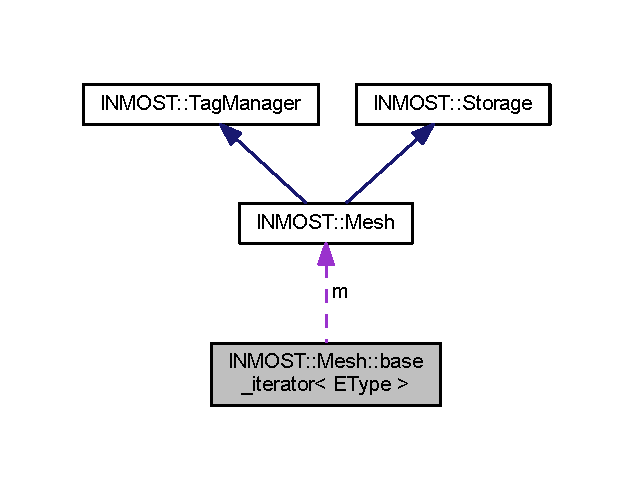
\includegraphics[width=304pt]{classINMOST_1_1Mesh_1_1base__iterator__coll__graph}
\end{center}
\end{figure}
\subsection*{Public Types}
\begin{DoxyCompactItemize}
\item 
\hypertarget{classINMOST_1_1Mesh_1_1base__iterator_a29cc18b3b80bca355984dc791f040f03}{typedef Handle\-Type $\ast$ {\bfseries pointer}}\label{classINMOST_1_1Mesh_1_1base__iterator_a29cc18b3b80bca355984dc791f040f03}

\item 
\hypertarget{classINMOST_1_1Mesh_1_1base__iterator_a67b7c0dba5f2926f55739d1e441347d8}{typedef Handle\-Type \& {\bfseries reference}}\label{classINMOST_1_1Mesh_1_1base__iterator_a67b7c0dba5f2926f55739d1e441347d8}

\item 
\hypertarget{classINMOST_1_1Mesh_1_1base__iterator_a6d47ff7ab477cc9c873c232236a860f0}{typedef Handle\-Type {\bfseries value\-\_\-type}}\label{classINMOST_1_1Mesh_1_1base__iterator_a6d47ff7ab477cc9c873c232236a860f0}

\item 
\hypertarget{classINMOST_1_1Mesh_1_1base__iterator_a83167a54e5fc607c5ce567420cef9614}{typedef ptrdiff\-\_\-t {\bfseries difference\-\_\-type}}\label{classINMOST_1_1Mesh_1_1base__iterator_a83167a54e5fc607c5ce567420cef9614}

\item 
\hypertarget{classINMOST_1_1Mesh_1_1base__iterator_af093745c78c6779d0c159a4671c1bd6b}{typedef \\*
std\-::bidirectional\-\_\-iterator\-\_\-tag {\bfseries iterator\-\_\-category}}\label{classINMOST_1_1Mesh_1_1base__iterator_af093745c78c6779d0c159a4671c1bd6b}

\end{DoxyCompactItemize}
\subsection*{Public Member Functions}
\begin{DoxyCompactItemize}
\item 
\hypertarget{classINMOST_1_1Mesh_1_1base__iterator_a75441532569b3b809bc2444aab2efc99}{{\bfseries base\-\_\-iterator} (const \hyperlink{classINMOST_1_1Mesh_1_1base__iterator}{base\-\_\-iterator} \&other)}\label{classINMOST_1_1Mesh_1_1base__iterator_a75441532569b3b809bc2444aab2efc99}

\item 
\hypertarget{classINMOST_1_1Mesh_1_1base__iterator_aa257e4d57452ffa1dfa478ae0362a5ec}{\hyperlink{classINMOST_1_1Mesh_1_1base__iterator}{base\-\_\-iterator} \& {\bfseries operator++} ()}\label{classINMOST_1_1Mesh_1_1base__iterator_aa257e4d57452ffa1dfa478ae0362a5ec}

\item 
\hypertarget{classINMOST_1_1Mesh_1_1base__iterator_a0b8431dc0e99a4ee5a307937beda8e25}{\-\_\-\-\_\-\-I\-N\-L\-I\-N\-E \hyperlink{classINMOST_1_1Mesh_1_1base__iterator}{base\-\_\-iterator} {\bfseries operator++} (int)}\label{classINMOST_1_1Mesh_1_1base__iterator_a0b8431dc0e99a4ee5a307937beda8e25}

\item 
\hypertarget{classINMOST_1_1Mesh_1_1base__iterator_ac5737f13780fd3b714fe869e1a17b46d}{\hyperlink{classINMOST_1_1Mesh_1_1base__iterator}{base\-\_\-iterator} \& {\bfseries operator-\/-\/} ()}\label{classINMOST_1_1Mesh_1_1base__iterator_ac5737f13780fd3b714fe869e1a17b46d}

\item 
\hypertarget{classINMOST_1_1Mesh_1_1base__iterator_a0fb6e373e1134d6a519b302eda3a00f2}{\-\_\-\-\_\-\-I\-N\-L\-I\-N\-E \hyperlink{classINMOST_1_1Mesh_1_1base__iterator}{base\-\_\-iterator} {\bfseries operator-\/-\/} (int)}\label{classINMOST_1_1Mesh_1_1base__iterator_a0fb6e373e1134d6a519b302eda3a00f2}

\item 
\hypertarget{classINMOST_1_1Mesh_1_1base__iterator_a8b0cef4064c2eef72fcabf2c01fd7fd4}{\-\_\-\-\_\-\-I\-N\-L\-I\-N\-E value\-\_\-type {\bfseries operator$\ast$} ()}\label{classINMOST_1_1Mesh_1_1base__iterator_a8b0cef4064c2eef72fcabf2c01fd7fd4}

\item 
\hypertarget{classINMOST_1_1Mesh_1_1base__iterator_a1b5d24fd44090fbe7d644d27551f2c31}{\-\_\-\-\_\-\-I\-N\-L\-I\-N\-E E\-Type {\bfseries operator-\/$>$} ()}\label{classINMOST_1_1Mesh_1_1base__iterator_a1b5d24fd44090fbe7d644d27551f2c31}

\item 
\hypertarget{classINMOST_1_1Mesh_1_1base__iterator_aac96de7fb038497df25304a8b6b54b88}{\-\_\-\-\_\-\-I\-N\-L\-I\-N\-E \hyperlink{classINMOST_1_1Mesh_1_1base__iterator}{base\-\_\-iterator} \& {\bfseries operator=} (\hyperlink{classINMOST_1_1Mesh_1_1base__iterator}{base\-\_\-iterator} const \&other)}\label{classINMOST_1_1Mesh_1_1base__iterator_aac96de7fb038497df25304a8b6b54b88}

\item 
\hypertarget{classINMOST_1_1Mesh_1_1base__iterator_a16a66bd28c52716193b4f5abe2c80ecb}{\-\_\-\-\_\-\-I\-N\-L\-I\-N\-E bool {\bfseries operator==} (const \hyperlink{classINMOST_1_1Mesh_1_1base__iterator}{base\-\_\-iterator} \&other) const }\label{classINMOST_1_1Mesh_1_1base__iterator_a16a66bd28c52716193b4f5abe2c80ecb}

\item 
\hypertarget{classINMOST_1_1Mesh_1_1base__iterator_a302b717ea1ea4b93f2ace1fd946e924c}{\-\_\-\-\_\-\-I\-N\-L\-I\-N\-E bool {\bfseries operator!=} (const \hyperlink{classINMOST_1_1Mesh_1_1base__iterator}{base\-\_\-iterator} \&other) const }\label{classINMOST_1_1Mesh_1_1base__iterator_a302b717ea1ea4b93f2ace1fd946e924c}

\item 
\hypertarget{classINMOST_1_1Mesh_1_1base__iterator_a51ab37f5cb8f1dfac387bb6a427afdba}{\-\_\-\-\_\-\-I\-N\-L\-I\-N\-E bool {\bfseries operator$<$} (const \hyperlink{classINMOST_1_1Mesh_1_1base__iterator}{base\-\_\-iterator} \&other) const }\label{classINMOST_1_1Mesh_1_1base__iterator_a51ab37f5cb8f1dfac387bb6a427afdba}

\item 
\hypertarget{classINMOST_1_1Mesh_1_1base__iterator_a28941bfac35634c87df66f5e60bcfc82}{\-\_\-\-\_\-\-I\-N\-L\-I\-N\-E bool {\bfseries operator$>$} (const \hyperlink{classINMOST_1_1Mesh_1_1base__iterator}{base\-\_\-iterator} \&other) const }\label{classINMOST_1_1Mesh_1_1base__iterator_a28941bfac35634c87df66f5e60bcfc82}

\item 
\hypertarget{classINMOST_1_1Mesh_1_1base__iterator_aa88279fde29ec02d77fa38c0a14f7eb0}{\-\_\-\-\_\-\-I\-N\-L\-I\-N\-E bool {\bfseries operator$<$=} (const \hyperlink{classINMOST_1_1Mesh_1_1base__iterator}{base\-\_\-iterator} \&other) const }\label{classINMOST_1_1Mesh_1_1base__iterator_aa88279fde29ec02d77fa38c0a14f7eb0}

\item 
\hypertarget{classINMOST_1_1Mesh_1_1base__iterator_a9396e8623464ec450ae43dbd8a3873cb}{\-\_\-\-\_\-\-I\-N\-L\-I\-N\-E bool {\bfseries operator$>$=} (const \hyperlink{classINMOST_1_1Mesh_1_1base__iterator}{base\-\_\-iterator} \&other) const }\label{classINMOST_1_1Mesh_1_1base__iterator_a9396e8623464ec450ae43dbd8a3873cb}

\item 
\hypertarget{classINMOST_1_1Mesh_1_1base__iterator_ab63bf9d545779dd580dd5674e6648d56}{void {\bfseries Print} ()}\label{classINMOST_1_1Mesh_1_1base__iterator_ab63bf9d545779dd580dd5674e6648d56}

\end{DoxyCompactItemize}
\subsection*{Protected Member Functions}
\begin{DoxyCompactItemize}
\item 
\hypertarget{classINMOST_1_1Mesh_1_1base__iterator_ad45d33a8c95bb3c2dcdb2de971fcb67c}{{\bfseries base\-\_\-iterator} (Element\-Type Types, \hyperlink{classINMOST_1_1Mesh}{Mesh} $\ast$mesh, bool last)}\label{classINMOST_1_1Mesh_1_1base__iterator_ad45d33a8c95bb3c2dcdb2de971fcb67c}

\item 
\hypertarget{classINMOST_1_1Mesh_1_1base__iterator_a18693b1b90ca884efb913f147e4a534d}{{\bfseries base\-\_\-iterator} (\hyperlink{classINMOST_1_1Mesh}{Mesh} $\ast$mesh)}\label{classINMOST_1_1Mesh_1_1base__iterator_a18693b1b90ca884efb913f147e4a534d}

\end{DoxyCompactItemize}
\subsection*{Protected Attributes}
\begin{DoxyCompactItemize}
\item 
\hypertarget{classINMOST_1_1Mesh_1_1base__iterator_a0f7bf7b7fe3ccda4bc725033cf31649c}{\hyperlink{classINMOST_1_1Mesh}{Mesh} $\ast$ {\bfseries m}}\label{classINMOST_1_1Mesh_1_1base__iterator_a0f7bf7b7fe3ccda4bc725033cf31649c}

\item 
\hypertarget{classINMOST_1_1Mesh_1_1base__iterator_aae3d8d36a48d43bb0d05248d0dd66dfe}{\hyperlink{classINMOST_1_1Storage_aec96942bc647417a801e2895b45964d2}{Storage\-::integer} {\bfseries lid}}\label{classINMOST_1_1Mesh_1_1base__iterator_aae3d8d36a48d43bb0d05248d0dd66dfe}

\item 
\hypertarget{classINMOST_1_1Mesh_1_1base__iterator_a9147c2e3d17f1f6f4680109bcc0742f7}{Element\-Type {\bfseries etype}}\label{classINMOST_1_1Mesh_1_1base__iterator_a9147c2e3d17f1f6f4680109bcc0742f7}

\item 
\hypertarget{classINMOST_1_1Mesh_1_1base__iterator_a401525dcecea1a9a1e9cee5528b5b9eb}{Element\-Type {\bfseries types}}\label{classINMOST_1_1Mesh_1_1base__iterator_a401525dcecea1a9a1e9cee5528b5b9eb}

\end{DoxyCompactItemize}
\subsection*{Friends}
\begin{DoxyCompactItemize}
\item 
\hypertarget{classINMOST_1_1Mesh_1_1base__iterator_ace57fc663c2a237871b404139d498227}{\hyperlink{classINMOST_1_1Mesh_1_1base__iterator}{iterator\-Storage} {\bfseries Mesh\-::\-Begin} (Element\-Type Types)}\label{classINMOST_1_1Mesh_1_1base__iterator_ace57fc663c2a237871b404139d498227}

\item 
\hypertarget{classINMOST_1_1Mesh_1_1base__iterator_a671347dcf7323a73f73369df292e2921}{\hyperlink{classINMOST_1_1Mesh_1_1base__iterator}{iterator\-Storage} {\bfseries Mesh\-::\-End} ()}\label{classINMOST_1_1Mesh_1_1base__iterator_a671347dcf7323a73f73369df292e2921}

\item 
\hypertarget{classINMOST_1_1Mesh_1_1base__iterator_a0c8442749f880e9d2f422d006c79ef71}{\hyperlink{classINMOST_1_1Mesh_1_1base__iterator}{iterator\-Element} {\bfseries Mesh\-::\-Begin\-Element} (Element\-Type Types)}\label{classINMOST_1_1Mesh_1_1base__iterator_a0c8442749f880e9d2f422d006c79ef71}

\item 
\hypertarget{classINMOST_1_1Mesh_1_1base__iterator_aa83708600787bd5225c452d3dcfd5168}{\hyperlink{classINMOST_1_1Mesh_1_1base__iterator}{iterator\-Element} {\bfseries Mesh\-::\-End\-Element} ()}\label{classINMOST_1_1Mesh_1_1base__iterator_aa83708600787bd5225c452d3dcfd5168}

\item 
\hypertarget{classINMOST_1_1Mesh_1_1base__iterator_af7da87f6d660dbd35bc32640ae820634}{\hyperlink{classINMOST_1_1Mesh_1_1base__iterator}{iterator\-Set} {\bfseries Mesh\-::\-Begin\-Set} ()}\label{classINMOST_1_1Mesh_1_1base__iterator_af7da87f6d660dbd35bc32640ae820634}

\item 
\hypertarget{classINMOST_1_1Mesh_1_1base__iterator_a1e4a2a3197ab564fcaee7ef3e3f099f7}{\hyperlink{classINMOST_1_1Mesh_1_1base__iterator}{iterator\-Set} {\bfseries Mesh\-::\-End\-Set} ()}\label{classINMOST_1_1Mesh_1_1base__iterator_a1e4a2a3197ab564fcaee7ef3e3f099f7}

\item 
\hypertarget{classINMOST_1_1Mesh_1_1base__iterator_a61a3ce93e48e34ab4ed84150da7ea603}{\hyperlink{classINMOST_1_1Mesh_1_1base__iterator}{iterator\-Cell} {\bfseries Mesh\-::\-Begin\-Cell} ()}\label{classINMOST_1_1Mesh_1_1base__iterator_a61a3ce93e48e34ab4ed84150da7ea603}

\item 
\hypertarget{classINMOST_1_1Mesh_1_1base__iterator_a40cec03b434c21da6b4f3956ce4db095}{\hyperlink{classINMOST_1_1Mesh_1_1base__iterator}{iterator\-Cell} {\bfseries Mesh\-::\-End\-Cell} ()}\label{classINMOST_1_1Mesh_1_1base__iterator_a40cec03b434c21da6b4f3956ce4db095}

\item 
\hypertarget{classINMOST_1_1Mesh_1_1base__iterator_a6632423ad3c8ddd98c28ff7e79350115}{\hyperlink{classINMOST_1_1Mesh_1_1base__iterator}{iterator\-Face} {\bfseries Mesh\-::\-Begin\-Face} ()}\label{classINMOST_1_1Mesh_1_1base__iterator_a6632423ad3c8ddd98c28ff7e79350115}

\item 
\hypertarget{classINMOST_1_1Mesh_1_1base__iterator_a577c85aa5221223cbaa7f7160a98541c}{\hyperlink{classINMOST_1_1Mesh_1_1base__iterator}{iterator\-Face} {\bfseries Mesh\-::\-End\-Face} ()}\label{classINMOST_1_1Mesh_1_1base__iterator_a577c85aa5221223cbaa7f7160a98541c}

\item 
\hypertarget{classINMOST_1_1Mesh_1_1base__iterator_ab4f08fbacc97e19eef3e2c77991b129d}{\hyperlink{classINMOST_1_1Mesh_1_1base__iterator}{iterator\-Edge} {\bfseries Mesh\-::\-Begin\-Edge} ()}\label{classINMOST_1_1Mesh_1_1base__iterator_ab4f08fbacc97e19eef3e2c77991b129d}

\item 
\hypertarget{classINMOST_1_1Mesh_1_1base__iterator_a25eb7f1127f5744c62f8dd652006f78e}{\hyperlink{classINMOST_1_1Mesh_1_1base__iterator}{iterator\-Edge} {\bfseries Mesh\-::\-End\-Edge} ()}\label{classINMOST_1_1Mesh_1_1base__iterator_a25eb7f1127f5744c62f8dd652006f78e}

\item 
\hypertarget{classINMOST_1_1Mesh_1_1base__iterator_a5094383ca2a8cff6c20e7cf8867d6def}{\hyperlink{classINMOST_1_1Mesh_1_1base__iterator}{iterator\-Node} {\bfseries Mesh\-::\-Begin\-Node} ()}\label{classINMOST_1_1Mesh_1_1base__iterator_a5094383ca2a8cff6c20e7cf8867d6def}

\item 
\hypertarget{classINMOST_1_1Mesh_1_1base__iterator_a6d6fc4d1b1d711a1a6be638c495fdd1d}{\hyperlink{classINMOST_1_1Mesh_1_1base__iterator}{iterator\-Node} {\bfseries Mesh\-::\-End\-Node} ()}\label{classINMOST_1_1Mesh_1_1base__iterator_a6d6fc4d1b1d711a1a6be638c495fdd1d}

\end{DoxyCompactItemize}


The documentation for this class was generated from the following file\-:\begin{DoxyCompactItemize}
\item 
inmost\-\_\-mesh.\-h\end{DoxyCompactItemize}

\hypertarget{classINMOST_1_1Mesh_1_1BulkComparator}{\section{I\-N\-M\-O\-S\-T\-:\-:Mesh\-:\-:Bulk\-Comparator Class Reference}
\label{classINMOST_1_1Mesh_1_1BulkComparator}\index{I\-N\-M\-O\-S\-T\-::\-Mesh\-::\-Bulk\-Comparator@{I\-N\-M\-O\-S\-T\-::\-Mesh\-::\-Bulk\-Comparator}}
}
\subsection*{Public Member Functions}
\begin{DoxyCompactItemize}
\item 
\hypertarget{classINMOST_1_1Mesh_1_1BulkComparator_afc7c8db127b3f4339adf7ef48d921923}{{\bfseries Bulk\-Comparator} (\hyperlink{classINMOST_1_1Mesh}{Mesh} $\ast$m, \hyperlink{classINMOST_1_1Tag}{Tag} t)}\label{classINMOST_1_1Mesh_1_1BulkComparator_afc7c8db127b3f4339adf7ef48d921923}

\item 
\hypertarget{classINMOST_1_1Mesh_1_1BulkComparator_a5e30b8afe1f6cccea77fae07026566db}{{\bfseries Bulk\-Comparator} (const \hyperlink{classINMOST_1_1Mesh_1_1BulkComparator}{Bulk\-Comparator} \&other)}\label{classINMOST_1_1Mesh_1_1BulkComparator_a5e30b8afe1f6cccea77fae07026566db}

\item 
\hypertarget{classINMOST_1_1Mesh_1_1BulkComparator_a179a1129355506893435dd45980ad85e}{\hyperlink{classINMOST_1_1Mesh_1_1BulkComparator}{Bulk\-Comparator} \& {\bfseries operator=} (\hyperlink{classINMOST_1_1Mesh_1_1BulkComparator}{Bulk\-Comparator} const \&other)}\label{classINMOST_1_1Mesh_1_1BulkComparator_a179a1129355506893435dd45980ad85e}

\item 
\hypertarget{classINMOST_1_1Mesh_1_1BulkComparator_a8bd2436e36d465c2f9c2984b55c83ccd}{bool {\bfseries operator()} (Handle\-Type a, Handle\-Type b) const }\label{classINMOST_1_1Mesh_1_1BulkComparator_a8bd2436e36d465c2f9c2984b55c83ccd}

\item 
\hypertarget{classINMOST_1_1Mesh_1_1BulkComparator_a6691985bca09a9ad66e3d6dc9fdd0068}{bool {\bfseries operator()} (Handle\-Type a, \hyperlink{classINMOST_1_1Storage_ae429556af77094077d212e0ac23c8cfc}{bulk} b) const }\label{classINMOST_1_1Mesh_1_1BulkComparator_a6691985bca09a9ad66e3d6dc9fdd0068}

\end{DoxyCompactItemize}


The documentation for this class was generated from the following file\-:\begin{DoxyCompactItemize}
\item 
inmost\-\_\-mesh.\-h\end{DoxyCompactItemize}

\hypertarget{classINMOST_1_1Mesh_1_1BulkDFComparator}{\section{I\-N\-M\-O\-S\-T\-:\-:Mesh\-:\-:Bulk\-D\-F\-Comparator Class Reference}
\label{classINMOST_1_1Mesh_1_1BulkDFComparator}\index{I\-N\-M\-O\-S\-T\-::\-Mesh\-::\-Bulk\-D\-F\-Comparator@{I\-N\-M\-O\-S\-T\-::\-Mesh\-::\-Bulk\-D\-F\-Comparator}}
}
\subsection*{Public Member Functions}
\begin{DoxyCompactItemize}
\item 
\hypertarget{classINMOST_1_1Mesh_1_1BulkDFComparator_a1ea561959bc8330c64ebde348246ef8f}{{\bfseries Bulk\-D\-F\-Comparator} (\hyperlink{classINMOST_1_1Mesh}{Mesh} $\ast$m, \hyperlink{classINMOST_1_1Tag}{Tag} t)}\label{classINMOST_1_1Mesh_1_1BulkDFComparator_a1ea561959bc8330c64ebde348246ef8f}

\item 
\hypertarget{classINMOST_1_1Mesh_1_1BulkDFComparator_a35287407077b8c2cb3ef9386fa703be4}{{\bfseries Bulk\-D\-F\-Comparator} (const \hyperlink{classINMOST_1_1Mesh_1_1BulkDFComparator}{Bulk\-D\-F\-Comparator} \&other)}\label{classINMOST_1_1Mesh_1_1BulkDFComparator_a35287407077b8c2cb3ef9386fa703be4}

\item 
\hypertarget{classINMOST_1_1Mesh_1_1BulkDFComparator_a5270c6dd150e328188630b282afd67dc}{\hyperlink{classINMOST_1_1Mesh_1_1BulkDFComparator}{Bulk\-D\-F\-Comparator} \& {\bfseries operator=} (\hyperlink{classINMOST_1_1Mesh_1_1BulkDFComparator}{Bulk\-D\-F\-Comparator} const \&other)}\label{classINMOST_1_1Mesh_1_1BulkDFComparator_a5270c6dd150e328188630b282afd67dc}

\item 
\hypertarget{classINMOST_1_1Mesh_1_1BulkDFComparator_a714397aff2fb2191ad02921b22fca995}{bool {\bfseries operator()} (Handle\-Type a, Handle\-Type b) const }\label{classINMOST_1_1Mesh_1_1BulkDFComparator_a714397aff2fb2191ad02921b22fca995}

\item 
\hypertarget{classINMOST_1_1Mesh_1_1BulkDFComparator_ab716d607a57a5c2e2f549d6639f97fff}{bool {\bfseries operator()} (Handle\-Type a, \hyperlink{classINMOST_1_1Storage_ae429556af77094077d212e0ac23c8cfc}{bulk} b) const }\label{classINMOST_1_1Mesh_1_1BulkDFComparator_ab716d607a57a5c2e2f549d6639f97fff}

\end{DoxyCompactItemize}


The documentation for this class was generated from the following file\-:\begin{DoxyCompactItemize}
\item 
inmost\-\_\-mesh.\-h\end{DoxyCompactItemize}

\hypertarget{classINMOST_1_1Cell}{\section{I\-N\-M\-O\-S\-T\-:\-:Cell Class Reference}
\label{classINMOST_1_1Cell}\index{I\-N\-M\-O\-S\-T\-::\-Cell@{I\-N\-M\-O\-S\-T\-::\-Cell}}
}


An interface for elements of type C\-E\-L\-L.  




{\ttfamily \#include $<$inmost\-\_\-mesh.\-h$>$}



Inheritance diagram for I\-N\-M\-O\-S\-T\-:\-:Cell\-:\nopagebreak
\begin{figure}[H]
\begin{center}
\leavevmode
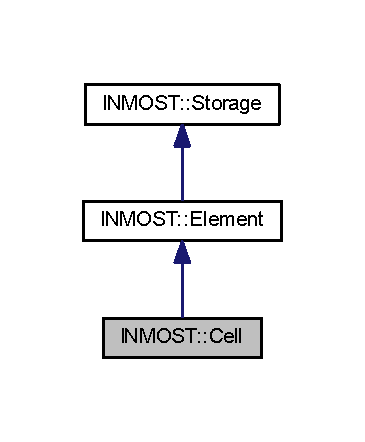
\includegraphics[width=175pt]{classINMOST_1_1Cell__inherit__graph}
\end{center}
\end{figure}


Collaboration diagram for I\-N\-M\-O\-S\-T\-:\-:Cell\-:\nopagebreak
\begin{figure}[H]
\begin{center}
\leavevmode
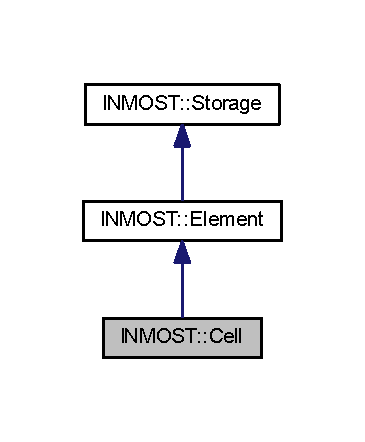
\includegraphics[width=175pt]{classINMOST_1_1Cell__coll__graph}
\end{center}
\end{figure}
\subsection*{Public Member Functions}
\begin{DoxyCompactItemize}
\item 
\hyperlink{classINMOST_1_1Cell_a5014e2a8bdc5c5e63d8f56203c446ff2}{Cell} ()
\begin{DoxyCompactList}\small\item\em Basic constructor. \end{DoxyCompactList}\item 
\hyperlink{classINMOST_1_1Cell_a6a5d747177264baf51981526d687160e}{Cell} (\hyperlink{classINMOST_1_1Mesh}{Mesh} $\ast$m, Handle\-Type h)
\begin{DoxyCompactList}\small\item\em Basic constructor with fixed handle. \end{DoxyCompactList}\item 
\hyperlink{classINMOST_1_1Cell_a3775295eb0087a53085e760ef15f7a5e}{Cell} (\hyperlink{classINMOST_1_1Mesh}{Mesh} $\ast$m, Handle\-Type $\ast$h)
\begin{DoxyCompactList}\small\item\em Basic constructor with an assignable handle. \end{DoxyCompactList}\item 
\hyperlink{classINMOST_1_1Cell_a2caed8dde9efdcd45bbab752beb1bc48}{Cell} (const \hyperlink{classINMOST_1_1Cell}{Cell} \&other)
\begin{DoxyCompactList}\small\item\em Copy constructor. \end{DoxyCompactList}\item 
\hyperlink{classINMOST_1_1Cell}{Cell} \& \hyperlink{classINMOST_1_1Cell_a42506f458c54cc177a56444d88b01770}{operator=} (\hyperlink{classINMOST_1_1Cell}{Cell} const \&other)
\begin{DoxyCompactList}\small\item\em Assignment operator. \end{DoxyCompactList}\item 
\hyperlink{classINMOST_1_1Cell}{Cell} $\ast$ \hyperlink{classINMOST_1_1Cell_a56ea16402b10b39c53c7c0fbc60ef748}{operator-\/$>$} ()
\begin{DoxyCompactList}\small\item\em Operator of dereference to pointer. \end{DoxyCompactList}\item 
const \hyperlink{classINMOST_1_1Cell}{Cell} $\ast$ \hyperlink{classINMOST_1_1Cell_a2f1b082d4303e9a36dcd7f37abf16698}{operator-\/$>$} () const 
\begin{DoxyCompactList}\small\item\em Operator of dereference to constant pointer. \end{DoxyCompactList}\item 
\hyperlink{classINMOST_1_1Cell}{Cell} \& \hyperlink{classINMOST_1_1Cell_ae7b259720c92912e8d267220f79e1ab5}{self} ()
\begin{DoxyCompactList}\small\item\em Get self-\/reference. \end{DoxyCompactList}\item 
const \hyperlink{classINMOST_1_1Cell}{Cell} \& \hyperlink{classINMOST_1_1Cell_ac283b04a07fdacfba61054cfc054f7bf}{self} () const 
\begin{DoxyCompactList}\small\item\em Get constant self-\/reference. \end{DoxyCompactList}\item 
\hyperlink{classINMOST_1_1ElementArray}{Element\-Array}$<$ \hyperlink{classINMOST_1_1Node}{Node} $>$ \hyperlink{classINMOST_1_1Cell_acc265095375df199a083a344d56e4645}{get\-Nodes} () const 
\begin{DoxyCompactList}\small\item\em Get all the nodes of the current cell. \end{DoxyCompactList}\item 
\hyperlink{classINMOST_1_1ElementArray}{Element\-Array}$<$ \hyperlink{classINMOST_1_1Edge}{Edge} $>$ \hyperlink{classINMOST_1_1Cell_ab0f9c4743826338a4df1b61b69b37c40}{get\-Edges} () const 
\begin{DoxyCompactList}\small\item\em Get all the edges of the current cell. \end{DoxyCompactList}\item 
\hyperlink{classINMOST_1_1ElementArray}{Element\-Array}$<$ \hyperlink{classINMOST_1_1Face}{Face} $>$ \hyperlink{classINMOST_1_1Cell_a85ccc42adbb161a36a866fcea0f961d2}{get\-Faces} () const 
\begin{DoxyCompactList}\small\item\em Get all the faces of the current cell. \end{DoxyCompactList}\item 
\hyperlink{classINMOST_1_1ElementArray}{Element\-Array}$<$ \hyperlink{classINMOST_1_1Node}{Node} $>$ \hyperlink{classINMOST_1_1Cell_a3ad5728090b1780f5c4226e5f73756f9}{get\-Nodes} (Marker\-Type mask, bool invert\-\_\-mask=false) const 
\begin{DoxyCompactList}\small\item\em Get the subset of the nodes of the current cell that are (not) marked by provided marker. \end{DoxyCompactList}\item 
\hyperlink{classINMOST_1_1ElementArray}{Element\-Array}$<$ \hyperlink{classINMOST_1_1Edge}{Edge} $>$ \hyperlink{classINMOST_1_1Cell_a93e527e5b5006011c78b0cd541129660}{get\-Edges} (Marker\-Type mask, bool invert\-\_\-mask=false) const 
\begin{DoxyCompactList}\small\item\em Get the subset of the edges of the current cell that are (not) marked by provided marker. \end{DoxyCompactList}\item 
\hyperlink{classINMOST_1_1ElementArray}{Element\-Array}$<$ \hyperlink{classINMOST_1_1Face}{Face} $>$ \hyperlink{classINMOST_1_1Cell_a631a1c2f3e429ecd32f7d8c60ee5b9c0}{get\-Faces} (Marker\-Type mask, bool invert\-\_\-mask=false) const 
\begin{DoxyCompactList}\small\item\em Get the subset of the faces of the current cell that are (not) marked by provided marker. \end{DoxyCompactList}\item 
bool \hyperlink{classINMOST_1_1Cell_afc84112c4d1f84b15799ffb91615cd30}{Check\-Edge\-Order} () const 
\begin{DoxyCompactList}\small\item\em Check that sequence of edges form a closed loop and each edge have a node that matches one of the nodes at the next edge. \end{DoxyCompactList}\item 
bool \hyperlink{classINMOST_1_1Cell_a84eaa268f8c3886e1164ea14715f2419}{Fix\-Edge\-Order} () const 
\begin{DoxyCompactList}\small\item\em Repair the sequence of edges so that each edge have node that matches one of the nodes at the next edge. \end{DoxyCompactList}\item 
\hyperlink{classINMOST_1_1Cell}{Cell} \hyperlink{classINMOST_1_1Cell_ab2fb575408f3ab8b60030e8e281ea4ed}{Neighbour} (\hyperlink{classINMOST_1_1Face}{Face} face) const 
\begin{DoxyCompactList}\small\item\em Get a cell that share a face with the current cell. \end{DoxyCompactList}\item 
\hyperlink{classINMOST_1_1ElementArray}{Element\-Array}$<$ \hyperlink{classINMOST_1_1Cell}{Cell} $>$ \hyperlink{classINMOST_1_1Cell_a47bc37b5c0fc45e2536f78787280fb4d}{Neighbouring\-Cells} () const 
\begin{DoxyCompactList}\small\item\em Get all cells that share the face with the current cell. \end{DoxyCompactList}\item 
bool \hyperlink{classINMOST_1_1Cell_a91562ae41d48c2fb99b824b7407659f5}{Inside} (const \hyperlink{classINMOST_1_1Storage_a853346784b4a5822a7fac54d8f10f805}{real} $\ast$point) const 
\begin{DoxyCompactList}\small\item\em Determine, if point lies inside element. \end{DoxyCompactList}\item 
\hyperlink{classINMOST_1_1Storage_a853346784b4a5822a7fac54d8f10f805}{real} \hyperlink{classINMOST_1_1Cell_ae0caec87803ddd108c4fb06decf69e18}{Volume} () const 
\begin{DoxyCompactList}\small\item\em Return volume of the cell. \end{DoxyCompactList}\item 
bool \hyperlink{classINMOST_1_1Cell_af07f9b3de49505cbe634c32882af2ac1}{Closure} () const 
\begin{DoxyCompactList}\small\item\em Test that faces of the cell form the closed set. \end{DoxyCompactList}\end{DoxyCompactItemize}
\subsection*{Static Public Member Functions}
\begin{DoxyCompactItemize}
\item 
static \hyperlink{classINMOST_1_1Cell}{Cell} \hyperlink{classINMOST_1_1Cell_a7f38ec05ba41d633d48bf05cdf2d0aad}{Unite\-Cells} (\hyperlink{classINMOST_1_1ElementArray}{Element\-Array}$<$ \hyperlink{classINMOST_1_1Cell}{Cell} $>$ \&cells, Marker\-Type del\-\_\-protect)
\begin{DoxyCompactList}\small\item\em Unite a set of given cells into one cell. \end{DoxyCompactList}\item 
static bool \hyperlink{classINMOST_1_1Cell_a874821b6ed2fd2907509146651312062}{Test\-Unite\-Cells} (const \hyperlink{classINMOST_1_1ElementArray}{Element\-Array}$<$ \hyperlink{classINMOST_1_1Cell}{Cell} $>$ \&cells, Marker\-Type del\-\_\-protect)
\begin{DoxyCompactList}\small\item\em Test that no marked element will be deleted during union of given cells. \end{DoxyCompactList}\item 
static \hyperlink{classINMOST_1_1ElementArray}{Element\-Array}$<$ \hyperlink{classINMOST_1_1Cell}{Cell} $>$ \hyperlink{classINMOST_1_1Cell_afd127d2e41a4b4362dc3399d9ac96a59}{Split\-Cell} (\hyperlink{classINMOST_1_1Cell}{Cell} cell, const \hyperlink{classINMOST_1_1ElementArray}{Element\-Array}$<$ \hyperlink{classINMOST_1_1Face}{Face} $>$ \&faces, Marker\-Type del\-\_\-protect)
\begin{DoxyCompactList}\small\item\em Separate a cell according to the set of provided faces. \end{DoxyCompactList}\item 
static bool \hyperlink{classINMOST_1_1Cell_ae48af9bae603442a3dccc81e39b18eb0}{Test\-Split\-Cell} (\hyperlink{classINMOST_1_1Cell}{Cell} cell, const \hyperlink{classINMOST_1_1ElementArray}{Element\-Array}$<$ \hyperlink{classINMOST_1_1Face}{Face} $>$ \&faces, Marker\-Type del\-\_\-protect)
\begin{DoxyCompactList}\small\item\em This functions checks is it possible to split the cell by the given set of faces without deleting marked elements. \end{DoxyCompactList}\end{DoxyCompactItemize}
\subsection*{Additional Inherited Members}


\subsection{Detailed Description}
An interface for elements of type C\-E\-L\-L. 

This interface carry the link to the mesh and the element's handle that represents position of the element's data in the mesh.

Interface provides some operations that can be done uniquely on the element of type C\-E\-L\-L.

For the basic set of operations on all of the elements check class \hyperlink{classINMOST_1_1Element}{Element}.

For the basic set of operations on the data of the element check class \hyperlink{classINMOST_1_1Storage}{Storage}.

You can obtain object of class \hyperlink{classINMOST_1_1Cell}{Cell} from Mesh\-::iterator\-Cell, in this case obtained object is always valid. Also you can get it through Mesh\-::\-Cell\-By\-Local\-I\-D, check with Element\-::is\-Valid to see whether you have obtained valid object. You can convert object of class \hyperlink{classINMOST_1_1Element}{Element} into object of class \hyperlink{classINMOST_1_1Cell}{Cell} by Element\-::get\-As\-Cell. In debug mode it will internally check that element is of type C\-E\-L\-L. You may compose object of class \hyperlink{classINMOST_1_1Cell}{Cell} by using constructor and specifing pointer to the mesh and providing element's handle. You can make handle with Compose\-Handle(\-C\-E\-L\-L,local\-\_\-id) function. 

\subsection{Constructor \& Destructor Documentation}
\hypertarget{classINMOST_1_1Cell_a5014e2a8bdc5c5e63d8f56203c446ff2}{\index{I\-N\-M\-O\-S\-T\-::\-Cell@{I\-N\-M\-O\-S\-T\-::\-Cell}!Cell@{Cell}}
\index{Cell@{Cell}!INMOST::Cell@{I\-N\-M\-O\-S\-T\-::\-Cell}}
\subsubsection[{Cell}]{\setlength{\rightskip}{0pt plus 5cm}I\-N\-M\-O\-S\-T\-::\-Cell\-::\-Cell (
\begin{DoxyParamCaption}
{}
\end{DoxyParamCaption}
)\hspace{0.3cm}{\ttfamily [inline]}}}\label{classINMOST_1_1Cell_a5014e2a8bdc5c5e63d8f56203c446ff2}


Basic constructor. 

Constructs invalid cell. \hypertarget{classINMOST_1_1Cell_a6a5d747177264baf51981526d687160e}{\index{I\-N\-M\-O\-S\-T\-::\-Cell@{I\-N\-M\-O\-S\-T\-::\-Cell}!Cell@{Cell}}
\index{Cell@{Cell}!INMOST::Cell@{I\-N\-M\-O\-S\-T\-::\-Cell}}
\subsubsection[{Cell}]{\setlength{\rightskip}{0pt plus 5cm}I\-N\-M\-O\-S\-T\-::\-Cell\-::\-Cell (
\begin{DoxyParamCaption}
\item[{{\bf Mesh} $\ast$}]{m, }
\item[{Handle\-Type}]{h}
\end{DoxyParamCaption}
)\hspace{0.3cm}{\ttfamily [inline]}}}\label{classINMOST_1_1Cell_a6a5d747177264baf51981526d687160e}


Basic constructor with fixed handle. 

When constructed this way, only handle within object may change.


\begin{DoxyParams}{Parameters}
{\em m} & Pointer to the mesh to which the element belongs. \\
\hline
{\em h} & Unique handle that describes position of the element within the mesh. \\
\hline
\end{DoxyParams}
\hypertarget{classINMOST_1_1Cell_a3775295eb0087a53085e760ef15f7a5e}{\index{I\-N\-M\-O\-S\-T\-::\-Cell@{I\-N\-M\-O\-S\-T\-::\-Cell}!Cell@{Cell}}
\index{Cell@{Cell}!INMOST::Cell@{I\-N\-M\-O\-S\-T\-::\-Cell}}
\subsubsection[{Cell}]{\setlength{\rightskip}{0pt plus 5cm}I\-N\-M\-O\-S\-T\-::\-Cell\-::\-Cell (
\begin{DoxyParamCaption}
\item[{{\bf Mesh} $\ast$}]{m, }
\item[{Handle\-Type $\ast$}]{h}
\end{DoxyParamCaption}
)\hspace{0.3cm}{\ttfamily [inline]}}}\label{classINMOST_1_1Cell_a3775295eb0087a53085e760ef15f7a5e}


Basic constructor with an assignable handle. 

When constructed this way, the provided memory location for handle will be modified on assignment.

The purpose of this function is to be used in various non-\/constant iterators of containers that allow underlaying contents to be changed.


\begin{DoxyParams}{Parameters}
{\em m} & Pointer to the mesh to which the element belongs. \\
\hline
{\em h} & Pointer to the handle that describes position of the element within mesh. \\
\hline
\end{DoxyParams}
\hypertarget{classINMOST_1_1Cell_a2caed8dde9efdcd45bbab752beb1bc48}{\index{I\-N\-M\-O\-S\-T\-::\-Cell@{I\-N\-M\-O\-S\-T\-::\-Cell}!Cell@{Cell}}
\index{Cell@{Cell}!INMOST::Cell@{I\-N\-M\-O\-S\-T\-::\-Cell}}
\subsubsection[{Cell}]{\setlength{\rightskip}{0pt plus 5cm}I\-N\-M\-O\-S\-T\-::\-Cell\-::\-Cell (
\begin{DoxyParamCaption}
\item[{const {\bf Cell} \&}]{other}
\end{DoxyParamCaption}
)\hspace{0.3cm}{\ttfamily [inline]}}}\label{classINMOST_1_1Cell_a2caed8dde9efdcd45bbab752beb1bc48}


Copy constructor. 

New object will inherit the assignment behavior of the initial object.


\begin{DoxyParams}{Parameters}
{\em other} & Object of type \hyperlink{classINMOST_1_1Cell}{Cell} to be duplicated. \\
\hline
\end{DoxyParams}


\subsection{Member Function Documentation}
\hypertarget{classINMOST_1_1Cell_afc84112c4d1f84b15799ffb91615cd30}{\index{I\-N\-M\-O\-S\-T\-::\-Cell@{I\-N\-M\-O\-S\-T\-::\-Cell}!Check\-Edge\-Order@{Check\-Edge\-Order}}
\index{Check\-Edge\-Order@{Check\-Edge\-Order}!INMOST::Cell@{I\-N\-M\-O\-S\-T\-::\-Cell}}
\subsubsection[{Check\-Edge\-Order}]{\setlength{\rightskip}{0pt plus 5cm}bool I\-N\-M\-O\-S\-T\-::\-Cell\-::\-Check\-Edge\-Order (
\begin{DoxyParamCaption}
{}
\end{DoxyParamCaption}
) const}}\label{classINMOST_1_1Cell_afc84112c4d1f84b15799ffb91615cd30}


Check that sequence of edges form a closed loop and each edge have a node that matches one of the nodes at the next edge. 

This function works for cells for which Element\-::\-Get\-Element\-Dimension returns 2.

\begin{DoxyReturn}{Returns}
True if edges form the correct closed loop.
\end{DoxyReturn}
\begin{DoxyRefDesc}{Todo}
\item[\hyperlink{todo__todo000003}{Todo}]
\begin{DoxyEnumerate}
\item Implement.
\item Use in topology check algorithms.
\item Use in \hyperlink{classINMOST_1_1Element_a96bd136b0f249c958fc8632553aa3b58}{Element\-::\-Connect}. 
\end{DoxyEnumerate}\end{DoxyRefDesc}
\hypertarget{classINMOST_1_1Cell_af07f9b3de49505cbe634c32882af2ac1}{\index{I\-N\-M\-O\-S\-T\-::\-Cell@{I\-N\-M\-O\-S\-T\-::\-Cell}!Closure@{Closure}}
\index{Closure@{Closure}!INMOST::Cell@{I\-N\-M\-O\-S\-T\-::\-Cell}}
\subsubsection[{Closure}]{\setlength{\rightskip}{0pt plus 5cm}bool I\-N\-M\-O\-S\-T\-::\-Cell\-::\-Closure (
\begin{DoxyParamCaption}
{}
\end{DoxyParamCaption}
) const}}\label{classINMOST_1_1Cell_af07f9b3de49505cbe634c32882af2ac1}


Test that faces of the cell form the closed set. 

This is automatically checked for if you activate N\-E\-E\-D\-\_\-\-T\-E\-S\-T\-\_\-\-C\-L\-O\-S\-U\-R\-E in \hyperlink{classINMOST_1_1Mesh_af9f578239d7b369ad4b1edb69eea24d2}{Mesh\-::\-Set\-Topology\-Check}. \begin{DoxyReturn}{Returns}
True if faces of the cell form the closed set, false otherwise. 
\end{DoxyReturn}
\hypertarget{classINMOST_1_1Cell_a84eaa268f8c3886e1164ea14715f2419}{\index{I\-N\-M\-O\-S\-T\-::\-Cell@{I\-N\-M\-O\-S\-T\-::\-Cell}!Fix\-Edge\-Order@{Fix\-Edge\-Order}}
\index{Fix\-Edge\-Order@{Fix\-Edge\-Order}!INMOST::Cell@{I\-N\-M\-O\-S\-T\-::\-Cell}}
\subsubsection[{Fix\-Edge\-Order}]{\setlength{\rightskip}{0pt plus 5cm}bool I\-N\-M\-O\-S\-T\-::\-Cell\-::\-Fix\-Edge\-Order (
\begin{DoxyParamCaption}
{}
\end{DoxyParamCaption}
) const}}\label{classINMOST_1_1Cell_a84eaa268f8c3886e1164ea14715f2419}


Repair the sequence of edges so that each edge have node that matches one of the nodes at the next edge. 

This function works for cells for which Element\-::\-Get\-Geometric\-Dimension returns 2.

This function may fail if all the edges does not form a closed loop.

\begin{DoxyReturn}{Returns}
True if edges were successfully reordered to form a closed loop.
\end{DoxyReturn}
\begin{DoxyRefDesc}{Todo}
\item[\hyperlink{todo__todo000004}{Todo}]
\begin{DoxyEnumerate}
\item Implement.
\item Use in topology check algorithms.
\item Use in \hyperlink{classINMOST_1_1Element_a96bd136b0f249c958fc8632553aa3b58}{Element\-::\-Connect}. 
\end{DoxyEnumerate}\end{DoxyRefDesc}
\hypertarget{classINMOST_1_1Cell_ab0f9c4743826338a4df1b61b69b37c40}{\index{I\-N\-M\-O\-S\-T\-::\-Cell@{I\-N\-M\-O\-S\-T\-::\-Cell}!get\-Edges@{get\-Edges}}
\index{get\-Edges@{get\-Edges}!INMOST::Cell@{I\-N\-M\-O\-S\-T\-::\-Cell}}
\subsubsection[{get\-Edges}]{\setlength{\rightskip}{0pt plus 5cm}{\bf Element\-Array}$<${\bf Edge}$>$ I\-N\-M\-O\-S\-T\-::\-Cell\-::get\-Edges (
\begin{DoxyParamCaption}
{}
\end{DoxyParamCaption}
) const\hspace{0.3cm}{\ttfamily [virtual]}}}\label{classINMOST_1_1Cell_ab0f9c4743826338a4df1b61b69b37c40}


Get all the edges of the current cell. 

This function traverses down the adjacency graph by two levels.

The order of the edges is unspecified.

W\-A\-R\-N\-I\-N\-G\-: Note that this function uses markers to check for duplication of edges in output array. This allows for faster algorithm, but will lead to penalties in shared parallel execution, since operations on markers are declared atomic. For atomic declaration to work you have to define U\-S\-E\-\_\-\-O\-M\-P during C\-Make configuration or in \hyperlink{inmost__common_8h_source}{inmost\-\_\-common.\-h}. If you attempt to use this function in shared parallel execution without U\-S\-E\-\_\-\-O\-M\-P you may expect side effects.

\begin{DoxyReturn}{Returns}
Set of edges that compose current cell.
\end{DoxyReturn}
\begin{DoxyRefDesc}{Todo}
\item[\hyperlink{todo__todo000002}{Todo}]One should thoroughly check three scenarios of function execution in shared parallel environment for different types of cells (simple tet/hex cells as well as complex polyhedral cells) and draw a conclusion on the best scenario for each condition. One of the development versions contains all the algorithms, ask for the files.
\begin{DoxyEnumerate}
\item Use of markers (current wariant).
\item Put all elements into array with duplications, then run std\-::sort and std\-::unique.
\item Put all elements into array, check for duplication by running through array. 
\end{DoxyEnumerate}\end{DoxyRefDesc}


Reimplemented from \hyperlink{classINMOST_1_1Element_a3ba56a19eeeb283864a006b0744fac4e}{I\-N\-M\-O\-S\-T\-::\-Element}.

\hypertarget{classINMOST_1_1Cell_a93e527e5b5006011c78b0cd541129660}{\index{I\-N\-M\-O\-S\-T\-::\-Cell@{I\-N\-M\-O\-S\-T\-::\-Cell}!get\-Edges@{get\-Edges}}
\index{get\-Edges@{get\-Edges}!INMOST::Cell@{I\-N\-M\-O\-S\-T\-::\-Cell}}
\subsubsection[{get\-Edges}]{\setlength{\rightskip}{0pt plus 5cm}{\bf Element\-Array}$<${\bf Edge}$>$ I\-N\-M\-O\-S\-T\-::\-Cell\-::get\-Edges (
\begin{DoxyParamCaption}
\item[{Marker\-Type}]{mask, }
\item[{bool}]{invert\-\_\-mask = {\ttfamily false}}
\end{DoxyParamCaption}
) const\hspace{0.3cm}{\ttfamily [virtual]}}}\label{classINMOST_1_1Cell_a93e527e5b5006011c78b0cd541129660}


Get the subset of the edges of the current cell that are (not) marked by provided marker. 

This function traverses down the adjacency graph by two levels.

The order of the edges is unspecified.

W\-A\-R\-N\-I\-N\-G\-: To work correctly in shared parallel environment this function requires U\-S\-E\-\_\-\-O\-M\-P to be defined in C\-Make or in \hyperlink{inmost__common_8h_source}{inmost\-\_\-common.\-h}.


\begin{DoxyParams}{Parameters}
{\em mask} & Marker that should be used to filter elements. \\
\hline
{\em invert\-\_\-mask} & If false then those elements that are marked will be taken, otherwise elements that are not marked will be taken. \\
\hline
\end{DoxyParams}
\begin{DoxyReturn}{Returns}
Set of the edges that compose current cell and (not) marked by marker. 
\end{DoxyReturn}


Reimplemented from \hyperlink{classINMOST_1_1Element}{I\-N\-M\-O\-S\-T\-::\-Element}.

\hypertarget{classINMOST_1_1Cell_a85ccc42adbb161a36a866fcea0f961d2}{\index{I\-N\-M\-O\-S\-T\-::\-Cell@{I\-N\-M\-O\-S\-T\-::\-Cell}!get\-Faces@{get\-Faces}}
\index{get\-Faces@{get\-Faces}!INMOST::Cell@{I\-N\-M\-O\-S\-T\-::\-Cell}}
\subsubsection[{get\-Faces}]{\setlength{\rightskip}{0pt plus 5cm}{\bf Element\-Array}$<${\bf Face}$>$ I\-N\-M\-O\-S\-T\-::\-Cell\-::get\-Faces (
\begin{DoxyParamCaption}
{}
\end{DoxyParamCaption}
) const\hspace{0.3cm}{\ttfamily [virtual]}}}\label{classINMOST_1_1Cell_a85ccc42adbb161a36a866fcea0f961d2}


Get all the faces of the current cell. 

This function traverses down the adjacency graph by one level.

The order of the faces returned by this function is preserved from the moment of the construction of the cell.

\begin{DoxyReturn}{Returns}
Set of faces that compose current cell. 
\end{DoxyReturn}


Reimplemented from \hyperlink{classINMOST_1_1Element_a2d9cc22d44f8d70c5b2876d84be6dfa5}{I\-N\-M\-O\-S\-T\-::\-Element}.

\hypertarget{classINMOST_1_1Cell_a631a1c2f3e429ecd32f7d8c60ee5b9c0}{\index{I\-N\-M\-O\-S\-T\-::\-Cell@{I\-N\-M\-O\-S\-T\-::\-Cell}!get\-Faces@{get\-Faces}}
\index{get\-Faces@{get\-Faces}!INMOST::Cell@{I\-N\-M\-O\-S\-T\-::\-Cell}}
\subsubsection[{get\-Faces}]{\setlength{\rightskip}{0pt plus 5cm}{\bf Element\-Array}$<${\bf Face}$>$ I\-N\-M\-O\-S\-T\-::\-Cell\-::get\-Faces (
\begin{DoxyParamCaption}
\item[{Marker\-Type}]{mask, }
\item[{bool}]{invert\-\_\-mask = {\ttfamily false}}
\end{DoxyParamCaption}
) const\hspace{0.3cm}{\ttfamily [virtual]}}}\label{classINMOST_1_1Cell_a631a1c2f3e429ecd32f7d8c60ee5b9c0}


Get the subset of the faces of the current cell that are (not) marked by provided marker. 

This function traverses down the adjacency graph by one level.

The order of the faces returned by this function is preserved from the moment of the construction of the cell.

W\-A\-R\-N\-I\-N\-G\-: To work correctly in shared parallel environment this function requires U\-S\-E\-\_\-\-O\-M\-P to be defined in C\-Make or in \hyperlink{inmost__common_8h_source}{inmost\-\_\-common.\-h}.


\begin{DoxyParams}{Parameters}
{\em mask} & Marker that should be used to filter elements. \\
\hline
{\em invert\-\_\-mask} & If false then those elements that are marked will be taken, otherwise elements that are not marked will be taken. \\
\hline
\end{DoxyParams}
\begin{DoxyReturn}{Returns}
Set of the faces that compose current cell and (not) marked by marker. 
\end{DoxyReturn}


Reimplemented from \hyperlink{classINMOST_1_1Element}{I\-N\-M\-O\-S\-T\-::\-Element}.

\hypertarget{classINMOST_1_1Cell_acc265095375df199a083a344d56e4645}{\index{I\-N\-M\-O\-S\-T\-::\-Cell@{I\-N\-M\-O\-S\-T\-::\-Cell}!get\-Nodes@{get\-Nodes}}
\index{get\-Nodes@{get\-Nodes}!INMOST::Cell@{I\-N\-M\-O\-S\-T\-::\-Cell}}
\subsubsection[{get\-Nodes}]{\setlength{\rightskip}{0pt plus 5cm}{\bf Element\-Array}$<${\bf Node}$>$ I\-N\-M\-O\-S\-T\-::\-Cell\-::get\-Nodes (
\begin{DoxyParamCaption}
{}
\end{DoxyParamCaption}
) const\hspace{0.3cm}{\ttfamily [virtual]}}}\label{classINMOST_1_1Cell_acc265095375df199a083a344d56e4645}


Get all the nodes of the current cell. 

This function traverses up the adjacency graph by one level.

The order of nodes will be preserved from the moment of the construction of the cell. When suggest\-\_\-nodes array is not supplied into the Mesh\-::\-Create\-Cell functions, then for known types the order of nodes follows V\-T\-K convention. For polyhedral cells the order is unspecified. When suggest\-\_\-nodes\-\_\-order was provided into Mesh\-::\-Create\-Cell then the order follows provided order.

\begin{DoxyReturn}{Returns}
Set of nodes that compose current cell. 
\end{DoxyReturn}


Reimplemented from \hyperlink{classINMOST_1_1Element_a00696ff8cd77491e1c4307cae166e92d}{I\-N\-M\-O\-S\-T\-::\-Element}.

\hypertarget{classINMOST_1_1Cell_a3ad5728090b1780f5c4226e5f73756f9}{\index{I\-N\-M\-O\-S\-T\-::\-Cell@{I\-N\-M\-O\-S\-T\-::\-Cell}!get\-Nodes@{get\-Nodes}}
\index{get\-Nodes@{get\-Nodes}!INMOST::Cell@{I\-N\-M\-O\-S\-T\-::\-Cell}}
\subsubsection[{get\-Nodes}]{\setlength{\rightskip}{0pt plus 5cm}{\bf Element\-Array}$<${\bf Node}$>$ I\-N\-M\-O\-S\-T\-::\-Cell\-::get\-Nodes (
\begin{DoxyParamCaption}
\item[{Marker\-Type}]{mask, }
\item[{bool}]{invert\-\_\-mask = {\ttfamily false}}
\end{DoxyParamCaption}
) const\hspace{0.3cm}{\ttfamily [virtual]}}}\label{classINMOST_1_1Cell_a3ad5728090b1780f5c4226e5f73756f9}


Get the subset of the nodes of the current cell that are (not) marked by provided marker. 

This function traverses up the adjacency graph by one level.

The order of nodes will be preserved from the moment of the construction of the cell. When suggest\-\_\-nodes array is not supplied into the Mesh\-::\-Create\-Cell functions, then for known types the order of nodes follows V\-T\-K convention. For polyhedral cells the order is unspecified. When suggest\-\_\-nodes\-\_\-order was provided into Mesh\-::\-Create\-Cell then the order follows provided order.

W\-A\-R\-N\-I\-N\-G\-: To work correctly in shared parallel environment this function requires U\-S\-E\-\_\-\-O\-M\-P to be defined in C\-Make or in \hyperlink{inmost__common_8h_source}{inmost\-\_\-common.\-h}.


\begin{DoxyParams}{Parameters}
{\em mask} & Marker that should be used to filter elements. \\
\hline
{\em invert\-\_\-mask} & If false then those elements that are marked will be taken, otherwise elements that are not marked will be taken. \\
\hline
\end{DoxyParams}
\begin{DoxyReturn}{Returns}
Set of the nodes that compose current cell and (not) marked by marker. 
\end{DoxyReturn}


Reimplemented from \hyperlink{classINMOST_1_1Element}{I\-N\-M\-O\-S\-T\-::\-Element}.

\hypertarget{classINMOST_1_1Cell_a91562ae41d48c2fb99b824b7407659f5}{\index{I\-N\-M\-O\-S\-T\-::\-Cell@{I\-N\-M\-O\-S\-T\-::\-Cell}!Inside@{Inside}}
\index{Inside@{Inside}!INMOST::Cell@{I\-N\-M\-O\-S\-T\-::\-Cell}}
\subsubsection[{Inside}]{\setlength{\rightskip}{0pt plus 5cm}bool I\-N\-M\-O\-S\-T\-::\-Cell\-::\-Inside (
\begin{DoxyParamCaption}
\item[{const {\bf real} $\ast$}]{point}
\end{DoxyParamCaption}
) const}}\label{classINMOST_1_1Cell_a91562ae41d48c2fb99b824b7407659f5}


Determine, if point lies inside element. 

Now it works only for 3-\/dimensional elements, at future it will be extended to support polygons and segments. 
\begin{DoxyParams}{Parameters}
{\em point} & coordinates of the point, it is assumed that number of the coordinates is the same as the number of dimensions in the mesh. \\
\hline
\end{DoxyParams}
\begin{DoxyReturn}{Returns}
returns true if points inside element, false otherwise 
\end{DoxyReturn}
\begin{DoxySeeAlso}{See Also}
\hyperlink{classINMOST_1_1Mesh_ae7b7567174f1da1fe8317eb8bb1fdc6c}{Mesh\-::\-Get\-Dimensions}
\end{DoxySeeAlso}
\begin{DoxyRefDesc}{Todo}
\item[\hyperlink{todo__todo000006}{Todo}]
\begin{DoxyEnumerate}
\item Should be checked or extended for 2d cells. (done, testing) 
\end{DoxyEnumerate}\end{DoxyRefDesc}
\hypertarget{classINMOST_1_1Cell_ab2fb575408f3ab8b60030e8e281ea4ed}{\index{I\-N\-M\-O\-S\-T\-::\-Cell@{I\-N\-M\-O\-S\-T\-::\-Cell}!Neighbour@{Neighbour}}
\index{Neighbour@{Neighbour}!INMOST::Cell@{I\-N\-M\-O\-S\-T\-::\-Cell}}
\subsubsection[{Neighbour}]{\setlength{\rightskip}{0pt plus 5cm}{\bf Cell} I\-N\-M\-O\-S\-T\-::\-Cell\-::\-Neighbour (
\begin{DoxyParamCaption}
\item[{{\bf Face}}]{face}
\end{DoxyParamCaption}
) const}}\label{classINMOST_1_1Cell_ab2fb575408f3ab8b60030e8e281ea4ed}


Get a cell that share a face with the current cell. 

Don't forget to check that the returned cell is valid. It would return invalid cell for boundary face.


\begin{DoxyParams}{Parameters}
{\em face} & A face of current cell for which neighbouring cell is determined. \\
\hline
\end{DoxyParams}
\begin{DoxyReturn}{Returns}
A cell that shares a given face with the current cell. 
\end{DoxyReturn}
\hypertarget{classINMOST_1_1Cell_a47bc37b5c0fc45e2536f78787280fb4d}{\index{I\-N\-M\-O\-S\-T\-::\-Cell@{I\-N\-M\-O\-S\-T\-::\-Cell}!Neighbouring\-Cells@{Neighbouring\-Cells}}
\index{Neighbouring\-Cells@{Neighbouring\-Cells}!INMOST::Cell@{I\-N\-M\-O\-S\-T\-::\-Cell}}
\subsubsection[{Neighbouring\-Cells}]{\setlength{\rightskip}{0pt plus 5cm}{\bf Element\-Array}$<${\bf Cell}$>$ I\-N\-M\-O\-S\-T\-::\-Cell\-::\-Neighbouring\-Cells (
\begin{DoxyParamCaption}
{}
\end{DoxyParamCaption}
) const}}\label{classINMOST_1_1Cell_a47bc37b5c0fc45e2536f78787280fb4d}


Get all cells that share the face with the current cell. 

\begin{DoxyReturn}{Returns}
Set of cells that share a face with the current cell. 
\end{DoxyReturn}
\hypertarget{classINMOST_1_1Cell_a56ea16402b10b39c53c7c0fbc60ef748}{\index{I\-N\-M\-O\-S\-T\-::\-Cell@{I\-N\-M\-O\-S\-T\-::\-Cell}!operator-\/$>$@{operator-\/$>$}}
\index{operator-\/$>$@{operator-\/$>$}!INMOST::Cell@{I\-N\-M\-O\-S\-T\-::\-Cell}}
\subsubsection[{operator-\/$>$}]{\setlength{\rightskip}{0pt plus 5cm}{\bf Cell}$\ast$ I\-N\-M\-O\-S\-T\-::\-Cell\-::operator-\/$>$ (
\begin{DoxyParamCaption}
{}
\end{DoxyParamCaption}
)\hspace{0.3cm}{\ttfamily [inline]}}}\label{classINMOST_1_1Cell_a56ea16402b10b39c53c7c0fbc60ef748}


Operator of dereference to pointer. 

This is needed for iterators to work properly.

\begin{DoxyReturn}{Returns}
Pointer to the current object. 
\end{DoxyReturn}
\hypertarget{classINMOST_1_1Cell_a2f1b082d4303e9a36dcd7f37abf16698}{\index{I\-N\-M\-O\-S\-T\-::\-Cell@{I\-N\-M\-O\-S\-T\-::\-Cell}!operator-\/$>$@{operator-\/$>$}}
\index{operator-\/$>$@{operator-\/$>$}!INMOST::Cell@{I\-N\-M\-O\-S\-T\-::\-Cell}}
\subsubsection[{operator-\/$>$}]{\setlength{\rightskip}{0pt plus 5cm}const {\bf Cell}$\ast$ I\-N\-M\-O\-S\-T\-::\-Cell\-::operator-\/$>$ (
\begin{DoxyParamCaption}
{}
\end{DoxyParamCaption}
) const\hspace{0.3cm}{\ttfamily [inline]}}}\label{classINMOST_1_1Cell_a2f1b082d4303e9a36dcd7f37abf16698}


Operator of dereference to constant pointer. 

This is needed for const\-\_\-iterators to work properly.

\begin{DoxyReturn}{Returns}
Constant pointer to the current object. 
\end{DoxyReturn}
\hypertarget{classINMOST_1_1Cell_a42506f458c54cc177a56444d88b01770}{\index{I\-N\-M\-O\-S\-T\-::\-Cell@{I\-N\-M\-O\-S\-T\-::\-Cell}!operator=@{operator=}}
\index{operator=@{operator=}!INMOST::Cell@{I\-N\-M\-O\-S\-T\-::\-Cell}}
\subsubsection[{operator=}]{\setlength{\rightskip}{0pt plus 5cm}{\bf Cell}\& I\-N\-M\-O\-S\-T\-::\-Cell\-::operator= (
\begin{DoxyParamCaption}
\item[{{\bf Cell} const \&}]{other}
\end{DoxyParamCaption}
)\hspace{0.3cm}{\ttfamily [inline]}}}\label{classINMOST_1_1Cell_a42506f458c54cc177a56444d88b01770}


Assignment operator. 

Assigned object will inherit the asignment behavior of the initial object only in case it was constructed without pointer to a handle. Otherwise it will only modify the memory location to which it points.


\begin{DoxyParams}{Parameters}
{\em other} & Object of type \hyperlink{classINMOST_1_1Cell}{Cell} to be duplicated. \\
\hline
\end{DoxyParams}
\begin{DoxyReturn}{Returns}
Reference to the current object. Assignment Operator. 
\end{DoxyReturn}
\hypertarget{classINMOST_1_1Cell_ae7b259720c92912e8d267220f79e1ab5}{\index{I\-N\-M\-O\-S\-T\-::\-Cell@{I\-N\-M\-O\-S\-T\-::\-Cell}!self@{self}}
\index{self@{self}!INMOST::Cell@{I\-N\-M\-O\-S\-T\-::\-Cell}}
\subsubsection[{self}]{\setlength{\rightskip}{0pt plus 5cm}{\bf Cell}\& I\-N\-M\-O\-S\-T\-::\-Cell\-::self (
\begin{DoxyParamCaption}
{}
\end{DoxyParamCaption}
)\hspace{0.3cm}{\ttfamily [inline]}}}\label{classINMOST_1_1Cell_ae7b259720c92912e8d267220f79e1ab5}


Get self-\/reference. 

Main purpose is to convert iterators into elements and to pass them as arguments of functions.

\begin{DoxyReturn}{Returns}
Constant reference to the current object. 
\end{DoxyReturn}
\hypertarget{classINMOST_1_1Cell_ac283b04a07fdacfba61054cfc054f7bf}{\index{I\-N\-M\-O\-S\-T\-::\-Cell@{I\-N\-M\-O\-S\-T\-::\-Cell}!self@{self}}
\index{self@{self}!INMOST::Cell@{I\-N\-M\-O\-S\-T\-::\-Cell}}
\subsubsection[{self}]{\setlength{\rightskip}{0pt plus 5cm}const {\bf Cell}\& I\-N\-M\-O\-S\-T\-::\-Cell\-::self (
\begin{DoxyParamCaption}
{}
\end{DoxyParamCaption}
) const\hspace{0.3cm}{\ttfamily [inline]}}}\label{classINMOST_1_1Cell_ac283b04a07fdacfba61054cfc054f7bf}


Get constant self-\/reference. 

Main purpose is to convert iterators into elements and to pass them as arguments of functions.

\begin{DoxyReturn}{Returns}
Reference to the current object. 
\end{DoxyReturn}
\hypertarget{classINMOST_1_1Cell_afd127d2e41a4b4362dc3399d9ac96a59}{\index{I\-N\-M\-O\-S\-T\-::\-Cell@{I\-N\-M\-O\-S\-T\-::\-Cell}!Split\-Cell@{Split\-Cell}}
\index{Split\-Cell@{Split\-Cell}!INMOST::Cell@{I\-N\-M\-O\-S\-T\-::\-Cell}}
\subsubsection[{Split\-Cell}]{\setlength{\rightskip}{0pt plus 5cm}static {\bf Element\-Array}$<${\bf Cell}$>$ I\-N\-M\-O\-S\-T\-::\-Cell\-::\-Split\-Cell (
\begin{DoxyParamCaption}
\item[{{\bf Cell}}]{cell, }
\item[{const {\bf Element\-Array}$<$ {\bf Face} $>$ \&}]{faces, }
\item[{Marker\-Type}]{del\-\_\-protect}
\end{DoxyParamCaption}
)\hspace{0.3cm}{\ttfamily [static]}}}\label{classINMOST_1_1Cell_afd127d2e41a4b4362dc3399d9ac96a59}


Separate a cell according to the set of provided faces. 

You should first separate all edges with new nodes by Edge\-::\-Split\-Edge, then faces with new edges by Face\-::\-Split\-Face and then create faces using new edges from faces of initial cell and optionally edges from inside of the cell. All faces are supposed to be internal with respect to the current cell. Internally this function will resolve geometry of new cells inside of the current cell by running through adjacency graph.


\begin{DoxyParams}{Parameters}
{\em cell} & A cell to be split. \\
\hline
{\em faces} & A set of faces, internal for current cell, that will be used for construction of new cells. \\
\hline
{\em del\-\_\-protect} & Marker that may be used to protect some elements from deletion by algorithm. Zero means no check. \\
\hline
\end{DoxyParams}
\begin{DoxyReturn}{Returns}
A set of new cells. 
\end{DoxyReturn}
\begin{DoxySeeAlso}{See Also}
Edge\-::\-Split\-Edge 

Face\-::\-Split\-Face
\end{DoxySeeAlso}
\begin{DoxyRefDesc}{Todo}
\item[\hyperlink{todo__todo000005}{Todo}]
\begin{DoxyEnumerate}
\item The algorithm inside is minimizing the size of the adjacency graph for each new cell. The correct behavior is to calculate volume of the cell for each adjacency graph and choose the graph with minimal volume. This requires calculation of volume for non-\/convex cells. For correct calculation of volume on non-\/convex cells one should find one face for which normal orientation can be clearly determined and then orient all edges of the cell with respect to the orientation of edges of this face and establish normals for all faces. Once the algorithm is implemented here it should be implemented in geometrical services or vice verse.
\item Probably the algorithm should minimize the volume and adjacency graph size altogether. Between the cells with smallest volume within some tolerance select those that have smallest adjacency graph. 
\end{DoxyEnumerate}\end{DoxyRefDesc}
\hypertarget{classINMOST_1_1Cell_ae48af9bae603442a3dccc81e39b18eb0}{\index{I\-N\-M\-O\-S\-T\-::\-Cell@{I\-N\-M\-O\-S\-T\-::\-Cell}!Test\-Split\-Cell@{Test\-Split\-Cell}}
\index{Test\-Split\-Cell@{Test\-Split\-Cell}!INMOST::Cell@{I\-N\-M\-O\-S\-T\-::\-Cell}}
\subsubsection[{Test\-Split\-Cell}]{\setlength{\rightskip}{0pt plus 5cm}static bool I\-N\-M\-O\-S\-T\-::\-Cell\-::\-Test\-Split\-Cell (
\begin{DoxyParamCaption}
\item[{{\bf Cell}}]{cell, }
\item[{const {\bf Element\-Array}$<$ {\bf Face} $>$ \&}]{faces, }
\item[{Marker\-Type}]{del\-\_\-protect}
\end{DoxyParamCaption}
)\hspace{0.3cm}{\ttfamily [static]}}}\label{classINMOST_1_1Cell_ae48af9bae603442a3dccc81e39b18eb0}


This functions checks is it possible to split the cell by the given set of faces without deleting marked elements. 


\begin{DoxyParams}{Parameters}
{\em cell} & A cell to be split. \\
\hline
{\em faces} & Set of faces, internal for current cell, that will be used for new cells. \\
\hline
{\em del\-\_\-protect} & Marker that may be used to protect some elements from deletion by algorithm. Zero means no check. \\
\hline
\end{DoxyParams}
\begin{DoxyReturn}{Returns}
True if possible, otherwise false. 
\end{DoxyReturn}
\hypertarget{classINMOST_1_1Cell_a874821b6ed2fd2907509146651312062}{\index{I\-N\-M\-O\-S\-T\-::\-Cell@{I\-N\-M\-O\-S\-T\-::\-Cell}!Test\-Unite\-Cells@{Test\-Unite\-Cells}}
\index{Test\-Unite\-Cells@{Test\-Unite\-Cells}!INMOST::Cell@{I\-N\-M\-O\-S\-T\-::\-Cell}}
\subsubsection[{Test\-Unite\-Cells}]{\setlength{\rightskip}{0pt plus 5cm}static bool I\-N\-M\-O\-S\-T\-::\-Cell\-::\-Test\-Unite\-Cells (
\begin{DoxyParamCaption}
\item[{const {\bf Element\-Array}$<$ {\bf Cell} $>$ \&}]{cells, }
\item[{Marker\-Type}]{del\-\_\-protect}
\end{DoxyParamCaption}
)\hspace{0.3cm}{\ttfamily [static]}}}\label{classINMOST_1_1Cell_a874821b6ed2fd2907509146651312062}


Test that no marked element will be deleted during union of given cells. 


\begin{DoxyParams}{Parameters}
{\em cells} & A set of cells to be united. \\
\hline
{\em del\-\_\-protect} & A marker that protects elements from deletion. Zero means no check. \\
\hline
\end{DoxyParams}
\begin{DoxyReturn}{Returns}
True if no element deleted, false otherwise. 
\end{DoxyReturn}
\hypertarget{classINMOST_1_1Cell_a7f38ec05ba41d633d48bf05cdf2d0aad}{\index{I\-N\-M\-O\-S\-T\-::\-Cell@{I\-N\-M\-O\-S\-T\-::\-Cell}!Unite\-Cells@{Unite\-Cells}}
\index{Unite\-Cells@{Unite\-Cells}!INMOST::Cell@{I\-N\-M\-O\-S\-T\-::\-Cell}}
\subsubsection[{Unite\-Cells}]{\setlength{\rightskip}{0pt plus 5cm}static {\bf Cell} I\-N\-M\-O\-S\-T\-::\-Cell\-::\-Unite\-Cells (
\begin{DoxyParamCaption}
\item[{{\bf Element\-Array}$<$ {\bf Cell} $>$ \&}]{cells, }
\item[{Marker\-Type}]{del\-\_\-protect}
\end{DoxyParamCaption}
)\hspace{0.3cm}{\ttfamily [static]}}}\label{classINMOST_1_1Cell_a7f38ec05ba41d633d48bf05cdf2d0aad}


Unite a set of given cells into one cell. 

This will create a cell whose faces are formed by symmetric difference of faces of given cells. If you specify a nonzero marker then the procedure will fail if any marked element have to be deleted during union. 
\begin{DoxyParams}{Parameters}
{\em cells} & A set of cells to be united. \\
\hline
{\em del\-\_\-protect} & A marker that protects elements from deletion. Zero means no check. \\
\hline
\end{DoxyParams}
\begin{DoxyReturn}{Returns}
A new cell. 
\end{DoxyReturn}
\hypertarget{classINMOST_1_1Cell_ae0caec87803ddd108c4fb06decf69e18}{\index{I\-N\-M\-O\-S\-T\-::\-Cell@{I\-N\-M\-O\-S\-T\-::\-Cell}!Volume@{Volume}}
\index{Volume@{Volume}!INMOST::Cell@{I\-N\-M\-O\-S\-T\-::\-Cell}}
\subsubsection[{Volume}]{\setlength{\rightskip}{0pt plus 5cm}{\bf real} I\-N\-M\-O\-S\-T\-::\-Cell\-::\-Volume (
\begin{DoxyParamCaption}
{}
\end{DoxyParamCaption}
) const}}\label{classINMOST_1_1Cell_ae0caec87803ddd108c4fb06decf69e18}


Return volume of the cell. 

Note that currently the volume for non-\/convex cells may be calculated incorrectly. \begin{DoxyRefDesc}{Todo}
\item[\hyperlink{todo__todo000007}{Todo}]
\begin{DoxyEnumerate}
\item Geometric services should correctly resolve volume for non-\/convex cells. 
\end{DoxyEnumerate}\end{DoxyRefDesc}


The documentation for this class was generated from the following file\-:\begin{DoxyCompactItemize}
\item 
inmost\-\_\-mesh.\-h\end{DoxyCompactItemize}

\hypertarget{classINMOST_1_1Mesh_1_1CentroidComparator}{\section{I\-N\-M\-O\-S\-T\-:\-:Mesh\-:\-:Centroid\-Comparator Class Reference}
\label{classINMOST_1_1Mesh_1_1CentroidComparator}\index{I\-N\-M\-O\-S\-T\-::\-Mesh\-::\-Centroid\-Comparator@{I\-N\-M\-O\-S\-T\-::\-Mesh\-::\-Centroid\-Comparator}}
}
\subsection*{Public Member Functions}
\begin{DoxyCompactItemize}
\item 
\hypertarget{classINMOST_1_1Mesh_1_1CentroidComparator_a673dcf3d8d6e6f0a76e3652727ccb439}{{\bfseries Centroid\-Comparator} (\hyperlink{classINMOST_1_1Mesh}{Mesh} $\ast$m)}\label{classINMOST_1_1Mesh_1_1CentroidComparator_a673dcf3d8d6e6f0a76e3652727ccb439}

\item 
\hypertarget{classINMOST_1_1Mesh_1_1CentroidComparator_a2765d9bbea2f0b8f3a6a1ba1f08db5ef}{{\bfseries Centroid\-Comparator} (const \hyperlink{classINMOST_1_1Mesh_1_1CentroidComparator}{Centroid\-Comparator} \&other)}\label{classINMOST_1_1Mesh_1_1CentroidComparator_a2765d9bbea2f0b8f3a6a1ba1f08db5ef}

\item 
\hypertarget{classINMOST_1_1Mesh_1_1CentroidComparator_a15d08fe8f5b5c53ae5d46e63525afcf1}{\hyperlink{classINMOST_1_1Mesh_1_1CentroidComparator}{Centroid\-Comparator} \& {\bfseries operator=} (\hyperlink{classINMOST_1_1Mesh_1_1CentroidComparator}{Centroid\-Comparator} const \&other)}\label{classINMOST_1_1Mesh_1_1CentroidComparator_a15d08fe8f5b5c53ae5d46e63525afcf1}

\item 
\hypertarget{classINMOST_1_1Mesh_1_1CentroidComparator_a615da7c67a7b9da7e007216c1f14dc17}{int {\bfseries Compare} (const \hyperlink{classINMOST_1_1Storage_a853346784b4a5822a7fac54d8f10f805}{real} $\ast$a, const \hyperlink{classINMOST_1_1Storage_a853346784b4a5822a7fac54d8f10f805}{real} $\ast$b) const }\label{classINMOST_1_1Mesh_1_1CentroidComparator_a615da7c67a7b9da7e007216c1f14dc17}

\item 
\hypertarget{classINMOST_1_1Mesh_1_1CentroidComparator_ac34a997d86c4a887e1806355ee3aa411}{bool {\bfseries operator()} (Handle\-Type a, Handle\-Type b) const }\label{classINMOST_1_1Mesh_1_1CentroidComparator_ac34a997d86c4a887e1806355ee3aa411}

\item 
\hypertarget{classINMOST_1_1Mesh_1_1CentroidComparator_a87611f52f9a70715d254613f3d580436}{bool {\bfseries operator()} (Handle\-Type a, const \hyperlink{classINMOST_1_1Storage_a853346784b4a5822a7fac54d8f10f805}{real} $\ast$b) const }\label{classINMOST_1_1Mesh_1_1CentroidComparator_a87611f52f9a70715d254613f3d580436}

\item 
\hypertarget{classINMOST_1_1Mesh_1_1CentroidComparator_af2bdd77d155ad58ab12908b49f8e2296}{bool {\bfseries operator()} (const \hyperlink{classINMOST_1_1Storage_a853346784b4a5822a7fac54d8f10f805}{real} $\ast$a, Handle\-Type b) const }\label{classINMOST_1_1Mesh_1_1CentroidComparator_af2bdd77d155ad58ab12908b49f8e2296}

\end{DoxyCompactItemize}


The documentation for this class was generated from the following file\-:\begin{DoxyCompactItemize}
\item 
inmost\-\_\-mesh.\-h\end{DoxyCompactItemize}

\hypertarget{classINMOST_1_1Storage_1_1reference__array_1_1const__iterator}{\section{I\-N\-M\-O\-S\-T\-:\-:Storage\-:\-:reference\-\_\-array\-:\-:const\-\_\-iterator Class Reference}
\label{classINMOST_1_1Storage_1_1reference__array_1_1const__iterator}\index{I\-N\-M\-O\-S\-T\-::\-Storage\-::reference\-\_\-array\-::const\-\_\-iterator@{I\-N\-M\-O\-S\-T\-::\-Storage\-::reference\-\_\-array\-::const\-\_\-iterator}}
}


Inheritance diagram for I\-N\-M\-O\-S\-T\-:\-:Storage\-:\-:reference\-\_\-array\-:\-:const\-\_\-iterator\-:\nopagebreak
\begin{figure}[H]
\begin{center}
\leavevmode
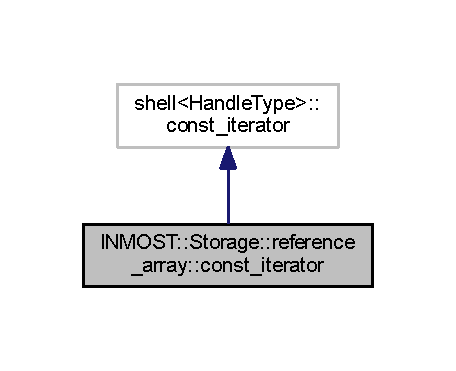
\includegraphics[width=219pt]{classINMOST_1_1Storage_1_1reference__array_1_1const__iterator__inherit__graph}
\end{center}
\end{figure}


Collaboration diagram for I\-N\-M\-O\-S\-T\-:\-:Storage\-:\-:reference\-\_\-array\-:\-:const\-\_\-iterator\-:\nopagebreak
\begin{figure}[H]
\begin{center}
\leavevmode
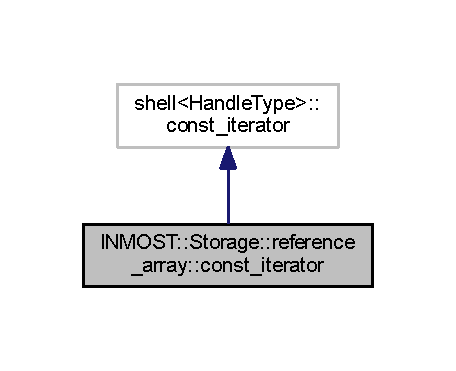
\includegraphics[width=219pt]{classINMOST_1_1Storage_1_1reference__array_1_1const__iterator__coll__graph}
\end{center}
\end{figure}
\subsection*{Public Member Functions}
\begin{DoxyCompactItemize}
\item 
\hypertarget{classINMOST_1_1Storage_1_1reference__array_1_1const__iterator_aee049aa18a46f40ef1852e2c46d59d02}{{\bfseries const\-\_\-iterator} (\hyperlink{classINMOST_1_1Mesh}{Mesh} $\ast$m, const shell$<$ Handle\-Type $>$\-::\hyperlink{classINMOST_1_1Storage_1_1reference__array_1_1const__iterator}{const\-\_\-iterator} \&other)}\label{classINMOST_1_1Storage_1_1reference__array_1_1const__iterator_aee049aa18a46f40ef1852e2c46d59d02}

\item 
\hypertarget{classINMOST_1_1Storage_1_1reference__array_1_1const__iterator_a95ce64fb4f1d6ad924dfae52fa9a9faa}{{\bfseries const\-\_\-iterator} (const \hyperlink{classINMOST_1_1Storage_1_1reference__array_1_1const__iterator}{const\-\_\-iterator} \&other)}\label{classINMOST_1_1Storage_1_1reference__array_1_1const__iterator_a95ce64fb4f1d6ad924dfae52fa9a9faa}

\item 
\hypertarget{classINMOST_1_1Storage_1_1reference__array_1_1const__iterator_a14703c26f3f90ec5eb0fa6a08fcd3789}{\hyperlink{classINMOST_1_1Storage_1_1reference__array_1_1const__iterator}{const\-\_\-iterator} \& {\bfseries operator=} (\hyperlink{classINMOST_1_1Storage_1_1reference__array_1_1const__iterator}{const\-\_\-iterator} const \&other)}\label{classINMOST_1_1Storage_1_1reference__array_1_1const__iterator_a14703c26f3f90ec5eb0fa6a08fcd3789}

\item 
\hypertarget{classINMOST_1_1Storage_1_1reference__array_1_1const__iterator_ade06e603cdc29abc2b86fabeb8741578}{\hyperlink{classINMOST_1_1Storage_1_1reference__array_1_1const__iterator}{const\-\_\-iterator} \& {\bfseries operator++} ()}\label{classINMOST_1_1Storage_1_1reference__array_1_1const__iterator_ade06e603cdc29abc2b86fabeb8741578}

\item 
\hypertarget{classINMOST_1_1Storage_1_1reference__array_1_1const__iterator_ae6602b970a8e782aab63d05d3b2786b7}{\hyperlink{classINMOST_1_1Storage_1_1reference__array_1_1const__iterator}{const\-\_\-iterator} {\bfseries operator++} (int)}\label{classINMOST_1_1Storage_1_1reference__array_1_1const__iterator_ae6602b970a8e782aab63d05d3b2786b7}

\item 
\hypertarget{classINMOST_1_1Storage_1_1reference__array_1_1const__iterator_a748977953b2a355cf4e7573d87e9398a}{\hyperlink{classINMOST_1_1Storage_1_1reference__array_1_1const__iterator}{const\-\_\-iterator} \& {\bfseries operator-\/-\/} ()}\label{classINMOST_1_1Storage_1_1reference__array_1_1const__iterator_a748977953b2a355cf4e7573d87e9398a}

\item 
\hypertarget{classINMOST_1_1Storage_1_1reference__array_1_1const__iterator_a0fe8966d0be2bd5f28283cfe187ed363}{\hyperlink{classINMOST_1_1Storage_1_1reference__array_1_1const__iterator}{const\-\_\-iterator} {\bfseries operator-\/-\/} (int)}\label{classINMOST_1_1Storage_1_1reference__array_1_1const__iterator_a0fe8966d0be2bd5f28283cfe187ed363}

\item 
\hypertarget{classINMOST_1_1Storage_1_1reference__array_1_1const__iterator_a9b315882528e3aed264dd976b2d76d2f}{\hyperlink{classINMOST_1_1Element}{Element} {\bfseries operator-\/$>$} ()}\label{classINMOST_1_1Storage_1_1reference__array_1_1const__iterator_a9b315882528e3aed264dd976b2d76d2f}

\end{DoxyCompactItemize}


The documentation for this class was generated from the following file\-:\begin{DoxyCompactItemize}
\item 
inmost\-\_\-mesh.\-h\end{DoxyCompactItemize}

\hypertarget{classINMOST_1_1ElementArray_1_1const__iterator}{\section{I\-N\-M\-O\-S\-T\-:\-:Element\-Array$<$ Storage\-Type $>$\-:\-:const\-\_\-iterator Class Reference}
\label{classINMOST_1_1ElementArray_1_1const__iterator}\index{I\-N\-M\-O\-S\-T\-::\-Element\-Array$<$ Storage\-Type $>$\-::const\-\_\-iterator@{I\-N\-M\-O\-S\-T\-::\-Element\-Array$<$ Storage\-Type $>$\-::const\-\_\-iterator}}
}


Inheritance diagram for I\-N\-M\-O\-S\-T\-:\-:Element\-Array$<$ Storage\-Type $>$\-:\-:const\-\_\-iterator\-:\nopagebreak
\begin{figure}[H]
\begin{center}
\leavevmode
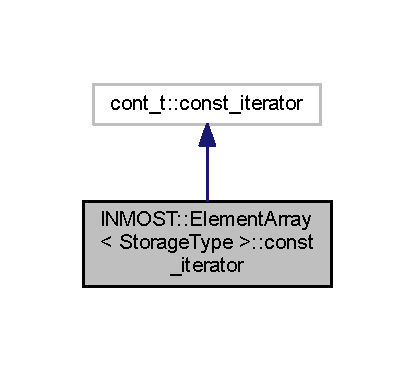
\includegraphics[width=199pt]{classINMOST_1_1ElementArray_1_1const__iterator__inherit__graph}
\end{center}
\end{figure}


Collaboration diagram for I\-N\-M\-O\-S\-T\-:\-:Element\-Array$<$ Storage\-Type $>$\-:\-:const\-\_\-iterator\-:\nopagebreak
\begin{figure}[H]
\begin{center}
\leavevmode
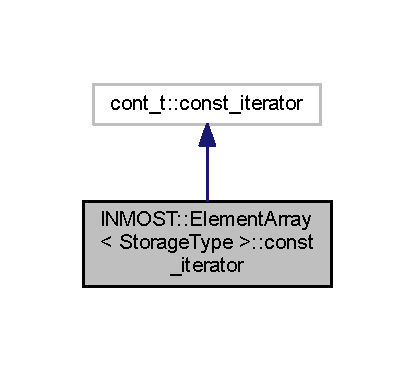
\includegraphics[width=199pt]{classINMOST_1_1ElementArray_1_1const__iterator__coll__graph}
\end{center}
\end{figure}
\subsection*{Public Member Functions}
\begin{DoxyCompactItemize}
\item 
\hypertarget{classINMOST_1_1ElementArray_1_1const__iterator_a45097d484ad220c130335829d26b618b}{{\bfseries const\-\_\-iterator} (\hyperlink{classINMOST_1_1Mesh}{Mesh} $\ast$m, const cont\-\_\-t\-::const\-\_\-iterator \&other)}\label{classINMOST_1_1ElementArray_1_1const__iterator_a45097d484ad220c130335829d26b618b}

\item 
\hypertarget{classINMOST_1_1ElementArray_1_1const__iterator_ae89b60d2097be1bc94e1002a5ff5014f}{{\bfseries const\-\_\-iterator} (const \hyperlink{classINMOST_1_1ElementArray_1_1const__iterator}{const\-\_\-iterator} \&other)}\label{classINMOST_1_1ElementArray_1_1const__iterator_ae89b60d2097be1bc94e1002a5ff5014f}

\item 
\hypertarget{classINMOST_1_1ElementArray_1_1const__iterator_a607f7e893b0b5c5a71aaacec237b1a64}{\hyperlink{classINMOST_1_1ElementArray_1_1const__iterator}{const\-\_\-iterator} \& {\bfseries operator++} ()}\label{classINMOST_1_1ElementArray_1_1const__iterator_a607f7e893b0b5c5a71aaacec237b1a64}

\item 
\hypertarget{classINMOST_1_1ElementArray_1_1const__iterator_aa685c5016fdfe19a0ad2e5d6091ad844}{\hyperlink{classINMOST_1_1ElementArray_1_1const__iterator}{const\-\_\-iterator} {\bfseries operator++} (int)}\label{classINMOST_1_1ElementArray_1_1const__iterator_aa685c5016fdfe19a0ad2e5d6091ad844}

\item 
\hypertarget{classINMOST_1_1ElementArray_1_1const__iterator_a08ec27e4e1fa64805c96f6a40fe37321}{\hyperlink{classINMOST_1_1ElementArray_1_1const__iterator}{const\-\_\-iterator} \& {\bfseries operator-\/-\/} ()}\label{classINMOST_1_1ElementArray_1_1const__iterator_a08ec27e4e1fa64805c96f6a40fe37321}

\item 
\hypertarget{classINMOST_1_1ElementArray_1_1const__iterator_ab7028a0fd30d20dc9902b02c74b04dc5}{\hyperlink{classINMOST_1_1ElementArray_1_1const__iterator}{const\-\_\-iterator} {\bfseries operator-\/-\/} (int)}\label{classINMOST_1_1ElementArray_1_1const__iterator_ab7028a0fd30d20dc9902b02c74b04dc5}

\item 
\hypertarget{classINMOST_1_1ElementArray_1_1const__iterator_a349b07e0cd1137c85e0b00ccc0a4d473}{\hyperlink{classINMOST_1_1ElementArray_1_1const__iterator}{const\-\_\-iterator} \& {\bfseries operator=} (\hyperlink{classINMOST_1_1ElementArray_1_1const__iterator}{const\-\_\-iterator} const \&other)}\label{classINMOST_1_1ElementArray_1_1const__iterator_a349b07e0cd1137c85e0b00ccc0a4d473}

\item 
\hypertarget{classINMOST_1_1ElementArray_1_1const__iterator_a9de46f6fd60eea5b0fee47b0a94e2e0c}{const Handle\-Type \& {\bfseries operator$\ast$} ()}\label{classINMOST_1_1ElementArray_1_1const__iterator_a9de46f6fd60eea5b0fee47b0a94e2e0c}

\item 
\hypertarget{classINMOST_1_1ElementArray_1_1const__iterator_a8e97fc3b963c256fd1bf27ce72bf08c3}{Storage\-Type {\bfseries operator-\/$>$} ()}\label{classINMOST_1_1ElementArray_1_1const__iterator_a8e97fc3b963c256fd1bf27ce72bf08c3}

\end{DoxyCompactItemize}


The documentation for this class was generated from the following file\-:\begin{DoxyCompactItemize}
\item 
inmost\-\_\-mesh.\-h\end{DoxyCompactItemize}

\hypertarget{classINMOST_1_1Storage_1_1reference__array_1_1const__reverse__iterator}{\section{I\-N\-M\-O\-S\-T\-:\-:Storage\-:\-:reference\-\_\-array\-:\-:const\-\_\-reverse\-\_\-iterator Class Reference}
\label{classINMOST_1_1Storage_1_1reference__array_1_1const__reverse__iterator}\index{I\-N\-M\-O\-S\-T\-::\-Storage\-::reference\-\_\-array\-::const\-\_\-reverse\-\_\-iterator@{I\-N\-M\-O\-S\-T\-::\-Storage\-::reference\-\_\-array\-::const\-\_\-reverse\-\_\-iterator}}
}


Inheritance diagram for I\-N\-M\-O\-S\-T\-:\-:Storage\-:\-:reference\-\_\-array\-:\-:const\-\_\-reverse\-\_\-iterator\-:
\nopagebreak
\begin{figure}[H]
\begin{center}
\leavevmode
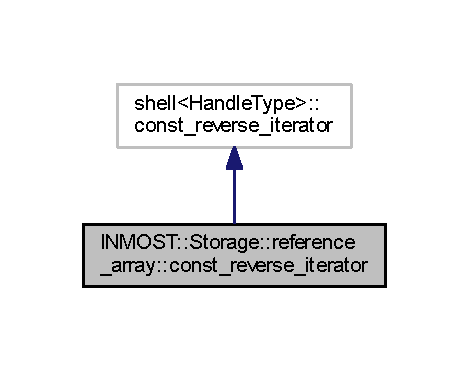
\includegraphics[width=225pt]{classINMOST_1_1Storage_1_1reference__array_1_1const__reverse__iterator__inherit__graph}
\end{center}
\end{figure}


Collaboration diagram for I\-N\-M\-O\-S\-T\-:\-:Storage\-:\-:reference\-\_\-array\-:\-:const\-\_\-reverse\-\_\-iterator\-:
\nopagebreak
\begin{figure}[H]
\begin{center}
\leavevmode
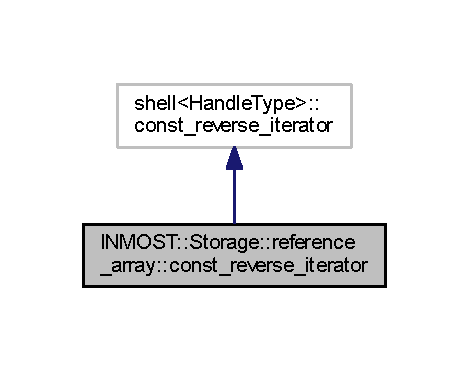
\includegraphics[width=225pt]{classINMOST_1_1Storage_1_1reference__array_1_1const__reverse__iterator__coll__graph}
\end{center}
\end{figure}
\subsection*{Public Member Functions}
\begin{DoxyCompactItemize}
\item 
\hypertarget{classINMOST_1_1Storage_1_1reference__array_1_1const__reverse__iterator_a5e2564fcf6ed29987cf1b778d015085b}{{\bfseries const\-\_\-reverse\-\_\-iterator} (\hyperlink{classINMOST_1_1Mesh}{Mesh} $\ast$m, const shell$<$ Handle\-Type $>$\-::\hyperlink{classINMOST_1_1Storage_1_1reference__array_1_1const__reverse__iterator}{const\-\_\-reverse\-\_\-iterator} \&other)}\label{classINMOST_1_1Storage_1_1reference__array_1_1const__reverse__iterator_a5e2564fcf6ed29987cf1b778d015085b}

\item 
\hypertarget{classINMOST_1_1Storage_1_1reference__array_1_1const__reverse__iterator_a26ed4296e84d2e0624873d070da3040d}{{\bfseries const\-\_\-reverse\-\_\-iterator} (const \hyperlink{classINMOST_1_1Storage_1_1reference__array_1_1const__reverse__iterator}{const\-\_\-reverse\-\_\-iterator} \&other)}\label{classINMOST_1_1Storage_1_1reference__array_1_1const__reverse__iterator_a26ed4296e84d2e0624873d070da3040d}

\item 
\hypertarget{classINMOST_1_1Storage_1_1reference__array_1_1const__reverse__iterator_a22380e551b393b0839c9521e7daee6bf}{\hyperlink{classINMOST_1_1Storage_1_1reference__array_1_1const__reverse__iterator}{const\-\_\-reverse\-\_\-iterator} \& {\bfseries operator=} (\hyperlink{classINMOST_1_1Storage_1_1reference__array_1_1const__reverse__iterator}{const\-\_\-reverse\-\_\-iterator} const \&other)}\label{classINMOST_1_1Storage_1_1reference__array_1_1const__reverse__iterator_a22380e551b393b0839c9521e7daee6bf}

\item 
\hypertarget{classINMOST_1_1Storage_1_1reference__array_1_1const__reverse__iterator_a89dc587d44b1f15b03e93d7c8ad1e267}{\hyperlink{classINMOST_1_1Storage_1_1reference__array_1_1const__reverse__iterator}{const\-\_\-reverse\-\_\-iterator} \& {\bfseries operator++} ()}\label{classINMOST_1_1Storage_1_1reference__array_1_1const__reverse__iterator_a89dc587d44b1f15b03e93d7c8ad1e267}

\item 
\hypertarget{classINMOST_1_1Storage_1_1reference__array_1_1const__reverse__iterator_ab59cc7799800c5ea03ecd5ee73efe065}{\hyperlink{classINMOST_1_1Storage_1_1reference__array_1_1const__reverse__iterator}{const\-\_\-reverse\-\_\-iterator} {\bfseries operator++} (int)}\label{classINMOST_1_1Storage_1_1reference__array_1_1const__reverse__iterator_ab59cc7799800c5ea03ecd5ee73efe065}

\item 
\hypertarget{classINMOST_1_1Storage_1_1reference__array_1_1const__reverse__iterator_af511e62d50470c187b78e2e02b55c2d6}{\hyperlink{classINMOST_1_1Storage_1_1reference__array_1_1const__reverse__iterator}{const\-\_\-reverse\-\_\-iterator} \& {\bfseries operator-\/-\/} ()}\label{classINMOST_1_1Storage_1_1reference__array_1_1const__reverse__iterator_af511e62d50470c187b78e2e02b55c2d6}

\item 
\hypertarget{classINMOST_1_1Storage_1_1reference__array_1_1const__reverse__iterator_a32e78a66fbbbb09b19a990ea5caae9c2}{\hyperlink{classINMOST_1_1Storage_1_1reference__array_1_1const__reverse__iterator}{const\-\_\-reverse\-\_\-iterator} {\bfseries operator-\/-\/} (int)}\label{classINMOST_1_1Storage_1_1reference__array_1_1const__reverse__iterator_a32e78a66fbbbb09b19a990ea5caae9c2}

\item 
\hypertarget{classINMOST_1_1Storage_1_1reference__array_1_1const__reverse__iterator_a41050b9776acf46dc919fceb36d409da}{\hyperlink{classINMOST_1_1Element}{Element} {\bfseries operator-\/$>$} ()}\label{classINMOST_1_1Storage_1_1reference__array_1_1const__reverse__iterator_a41050b9776acf46dc919fceb36d409da}

\end{DoxyCompactItemize}


The documentation for this class was generated from the following file\-:\begin{DoxyCompactItemize}
\item 
inmost\-\_\-mesh.\-h\end{DoxyCompactItemize}

\hypertarget{classINMOST_1_1ElementArray_1_1const__reverse__iterator}{\section{I\-N\-M\-O\-S\-T\-:\-:Element\-Array$<$ Storage\-Type $>$\-:\-:const\-\_\-reverse\-\_\-iterator Class Reference}
\label{classINMOST_1_1ElementArray_1_1const__reverse__iterator}\index{I\-N\-M\-O\-S\-T\-::\-Element\-Array$<$ Storage\-Type $>$\-::const\-\_\-reverse\-\_\-iterator@{I\-N\-M\-O\-S\-T\-::\-Element\-Array$<$ Storage\-Type $>$\-::const\-\_\-reverse\-\_\-iterator}}
}


Inheritance diagram for I\-N\-M\-O\-S\-T\-:\-:Element\-Array$<$ Storage\-Type $>$\-:\-:const\-\_\-reverse\-\_\-iterator\-:\nopagebreak
\begin{figure}[H]
\begin{center}
\leavevmode
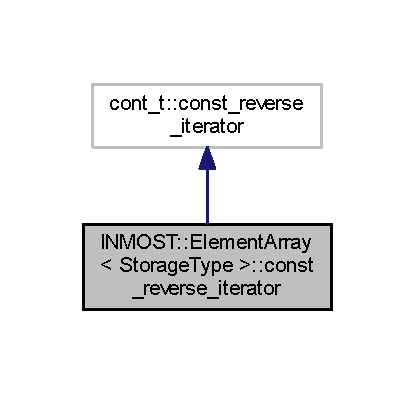
\includegraphics[width=199pt]{classINMOST_1_1ElementArray_1_1const__reverse__iterator__inherit__graph}
\end{center}
\end{figure}


Collaboration diagram for I\-N\-M\-O\-S\-T\-:\-:Element\-Array$<$ Storage\-Type $>$\-:\-:const\-\_\-reverse\-\_\-iterator\-:\nopagebreak
\begin{figure}[H]
\begin{center}
\leavevmode
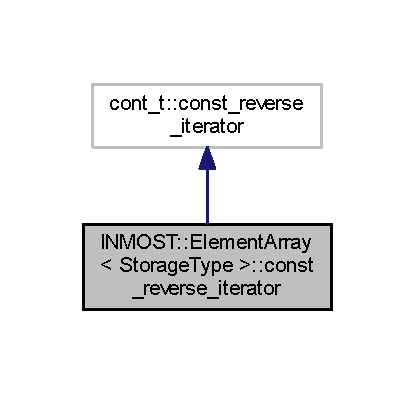
\includegraphics[width=199pt]{classINMOST_1_1ElementArray_1_1const__reverse__iterator__coll__graph}
\end{center}
\end{figure}
\subsection*{Public Member Functions}
\begin{DoxyCompactItemize}
\item 
\hypertarget{classINMOST_1_1ElementArray_1_1const__reverse__iterator_a037f9eec05ca80423cd9b9d6b3457048}{{\bfseries const\-\_\-reverse\-\_\-iterator} (\hyperlink{classINMOST_1_1Mesh}{Mesh} $\ast$m, const cont\-\_\-t\-::const\-\_\-reverse\-\_\-iterator \&other)}\label{classINMOST_1_1ElementArray_1_1const__reverse__iterator_a037f9eec05ca80423cd9b9d6b3457048}

\item 
\hypertarget{classINMOST_1_1ElementArray_1_1const__reverse__iterator_abf0f45810cb52f5d1090fc0b796c81cf}{{\bfseries const\-\_\-reverse\-\_\-iterator} (const \hyperlink{classINMOST_1_1ElementArray_1_1const__reverse__iterator}{const\-\_\-reverse\-\_\-iterator} \&other)}\label{classINMOST_1_1ElementArray_1_1const__reverse__iterator_abf0f45810cb52f5d1090fc0b796c81cf}

\item 
\hypertarget{classINMOST_1_1ElementArray_1_1const__reverse__iterator_a3525dcb7a3c19446311fb8874d5c2ab9}{\hyperlink{classINMOST_1_1ElementArray_1_1const__reverse__iterator}{const\-\_\-reverse\-\_\-iterator} \& {\bfseries operator++} ()}\label{classINMOST_1_1ElementArray_1_1const__reverse__iterator_a3525dcb7a3c19446311fb8874d5c2ab9}

\item 
\hypertarget{classINMOST_1_1ElementArray_1_1const__reverse__iterator_a10fe3e91cb322c3d60ad39457b34e5a8}{\hyperlink{classINMOST_1_1ElementArray_1_1const__reverse__iterator}{const\-\_\-reverse\-\_\-iterator} {\bfseries operator++} (int)}\label{classINMOST_1_1ElementArray_1_1const__reverse__iterator_a10fe3e91cb322c3d60ad39457b34e5a8}

\item 
\hypertarget{classINMOST_1_1ElementArray_1_1const__reverse__iterator_af051be64b3c28d4e2d7c66ec910a9b3b}{\hyperlink{classINMOST_1_1ElementArray_1_1const__reverse__iterator}{const\-\_\-reverse\-\_\-iterator} \& {\bfseries operator-\/-\/} ()}\label{classINMOST_1_1ElementArray_1_1const__reverse__iterator_af051be64b3c28d4e2d7c66ec910a9b3b}

\item 
\hypertarget{classINMOST_1_1ElementArray_1_1const__reverse__iterator_a16c2693ac33c483b26edd8e9de4b16a7}{\hyperlink{classINMOST_1_1ElementArray_1_1const__reverse__iterator}{const\-\_\-reverse\-\_\-iterator} {\bfseries operator-\/-\/} (int)}\label{classINMOST_1_1ElementArray_1_1const__reverse__iterator_a16c2693ac33c483b26edd8e9de4b16a7}

\item 
\hypertarget{classINMOST_1_1ElementArray_1_1const__reverse__iterator_a649b02b1a0cce701e84a2756062bedd5}{\hyperlink{classINMOST_1_1ElementArray_1_1const__reverse__iterator}{const\-\_\-reverse\-\_\-iterator} \& {\bfseries operator=} (\hyperlink{classINMOST_1_1ElementArray_1_1const__reverse__iterator}{const\-\_\-reverse\-\_\-iterator} const \&other)}\label{classINMOST_1_1ElementArray_1_1const__reverse__iterator_a649b02b1a0cce701e84a2756062bedd5}

\item 
\hypertarget{classINMOST_1_1ElementArray_1_1const__reverse__iterator_ab7c6d555cc57f6227e46ec3f24431667}{const Handle\-Type \& {\bfseries operator$\ast$} ()}\label{classINMOST_1_1ElementArray_1_1const__reverse__iterator_ab7c6d555cc57f6227e46ec3f24431667}

\item 
\hypertarget{classINMOST_1_1ElementArray_1_1const__reverse__iterator_a333f2f1c103e22d487184f659b0a210f}{Storage\-Type {\bfseries operator-\/$>$} ()}\label{classINMOST_1_1ElementArray_1_1const__reverse__iterator_a333f2f1c103e22d487184f659b0a210f}

\end{DoxyCompactItemize}


The documentation for this class was generated from the following file\-:\begin{DoxyCompactItemize}
\item 
inmost\-\_\-mesh.\-h\end{DoxyCompactItemize}

\hypertarget{classINMOST_1_1Edge}{\section{I\-N\-M\-O\-S\-T\-:\-:Edge Class Reference}
\label{classINMOST_1_1Edge}\index{I\-N\-M\-O\-S\-T\-::\-Edge@{I\-N\-M\-O\-S\-T\-::\-Edge}}
}


Inheritance diagram for I\-N\-M\-O\-S\-T\-:\-:Edge\-:
\nopagebreak
\begin{figure}[H]
\begin{center}
\leavevmode
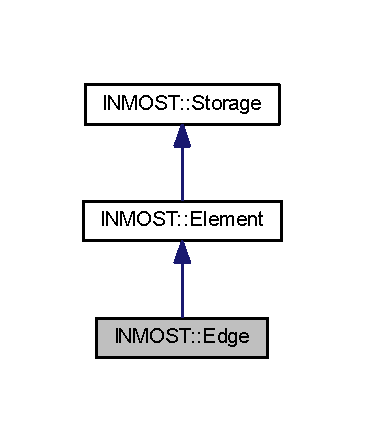
\includegraphics[width=175pt]{classINMOST_1_1Edge__inherit__graph}
\end{center}
\end{figure}


Collaboration diagram for I\-N\-M\-O\-S\-T\-:\-:Edge\-:
\nopagebreak
\begin{figure}[H]
\begin{center}
\leavevmode
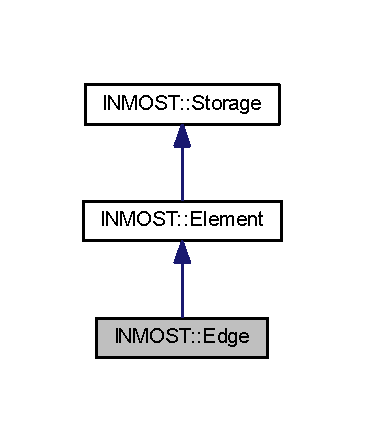
\includegraphics[width=175pt]{classINMOST_1_1Edge__coll__graph}
\end{center}
\end{figure}
\subsection*{Public Member Functions}
\begin{DoxyCompactItemize}
\item 
\hypertarget{classINMOST_1_1Edge_a5304345db2e5281455e2ef574d8ded70}{{\bfseries Edge} (const \hyperlink{classINMOST_1_1Edge}{Edge} \&other)}\label{classINMOST_1_1Edge_a5304345db2e5281455e2ef574d8ded70}

\item 
\hypertarget{classINMOST_1_1Edge_ae963d37a92085320893d846226c3027d}{{\bfseries Edge} (\hyperlink{classINMOST_1_1Mesh}{Mesh} $\ast$m, Handle\-Type h)}\label{classINMOST_1_1Edge_ae963d37a92085320893d846226c3027d}

\item 
\hypertarget{classINMOST_1_1Edge_aaaae84f52183a0faa90259d0020c0a39}{{\bfseries Edge} (\hyperlink{classINMOST_1_1Mesh}{Mesh} $\ast$m, Handle\-Type $\ast$h)}\label{classINMOST_1_1Edge_aaaae84f52183a0faa90259d0020c0a39}

\item 
\hypertarget{classINMOST_1_1Edge_a94ce93c2543797423d9505bce0ba77a8}{\hyperlink{classINMOST_1_1Edge}{Edge} \& {\bfseries operator=} (\hyperlink{classINMOST_1_1Edge}{Edge} const \&other)}\label{classINMOST_1_1Edge_a94ce93c2543797423d9505bce0ba77a8}

\item 
\hypertarget{classINMOST_1_1Edge_a55a79bd76daa99a5b27e5e47a179b318}{\hyperlink{classINMOST_1_1Edge}{Edge} $\ast$ {\bfseries operator-\/$>$} ()}\label{classINMOST_1_1Edge_a55a79bd76daa99a5b27e5e47a179b318}

\item 
\hypertarget{classINMOST_1_1Edge_a6e0a5b2c149f6da32e29a1381a9fea2b}{const \hyperlink{classINMOST_1_1Edge}{Edge} $\ast$ {\bfseries operator-\/$>$} () const }\label{classINMOST_1_1Edge_a6e0a5b2c149f6da32e29a1381a9fea2b}

\item 
\hypertarget{classINMOST_1_1Edge_ae49901107845bc2e4221018efea735bf}{\hyperlink{classINMOST_1_1Edge}{Edge} \& {\bfseries self} ()}\label{classINMOST_1_1Edge_ae49901107845bc2e4221018efea735bf}

\item 
\hypertarget{classINMOST_1_1Edge_a96dd80d27987140428b1f047e56d5549}{const \hyperlink{classINMOST_1_1Edge}{Edge} \& {\bfseries self} () const }\label{classINMOST_1_1Edge_a96dd80d27987140428b1f047e56d5549}

\item 
\hyperlink{classINMOST_1_1ElementArray}{Element\-Array}$<$ \hyperlink{classINMOST_1_1Node}{Node} $>$ \hyperlink{classINMOST_1_1Edge_a2e9e02817c50da41d366d9d89ff45bb8}{get\-Nodes} () const 
\begin{DoxyCompactList}\small\item\em Retrieve all the nodes of the element. \end{DoxyCompactList}\item 
\hyperlink{classINMOST_1_1ElementArray}{Element\-Array}$<$ \hyperlink{classINMOST_1_1Face}{Face} $>$ \hyperlink{classINMOST_1_1Edge_abfe4ce06477cfa404306c716d026d2ed}{get\-Faces} () const 
\begin{DoxyCompactList}\small\item\em Retrieve all the faces of the element. \end{DoxyCompactList}\item 
\hyperlink{classINMOST_1_1ElementArray}{Element\-Array}$<$ \hyperlink{classINMOST_1_1Cell}{Cell} $>$ \hyperlink{classINMOST_1_1Edge_ab38cdf43f623abcc12b0befbfac27b90}{get\-Cells} () const 
\begin{DoxyCompactList}\small\item\em Return all the cells of the element. \end{DoxyCompactList}\item 
\hypertarget{classINMOST_1_1Edge_a054c2768b16442babf7021046b3e6449}{\hyperlink{classINMOST_1_1ElementArray}{Element\-Array}$<$ \hyperlink{classINMOST_1_1Node}{Node} $>$ {\bfseries get\-Nodes} (Marker\-Type mask, bool invert\-\_\-mask=false) const }\label{classINMOST_1_1Edge_a054c2768b16442babf7021046b3e6449}

\item 
\hypertarget{classINMOST_1_1Edge_a62432abd01305826fa8506313b26a644}{\hyperlink{classINMOST_1_1ElementArray}{Element\-Array}$<$ \hyperlink{classINMOST_1_1Face}{Face} $>$ {\bfseries get\-Faces} (Marker\-Type mask, bool invert\-\_\-mask=false) const }\label{classINMOST_1_1Edge_a62432abd01305826fa8506313b26a644}

\item 
\hypertarget{classINMOST_1_1Edge_adc1db1a972137a0a1afe4bd607c54944}{\hyperlink{classINMOST_1_1ElementArray}{Element\-Array}$<$ \hyperlink{classINMOST_1_1Cell}{Cell} $>$ {\bfseries get\-Cells} (Marker\-Type mask, bool invert\-\_\-mask=false) const }\label{classINMOST_1_1Edge_adc1db1a972137a0a1afe4bd607c54944}

\item 
\hypertarget{classINMOST_1_1Edge_ad4a038ca78494621360e316c7eb4d2f7}{\hyperlink{classINMOST_1_1Node}{Node} {\bfseries get\-Beg} () const }\label{classINMOST_1_1Edge_ad4a038ca78494621360e316c7eb4d2f7}

\item 
\hypertarget{classINMOST_1_1Edge_a70191d91caf80e248728814c65f32573}{\hyperlink{classINMOST_1_1Node}{Node} {\bfseries get\-End} () const }\label{classINMOST_1_1Edge_a70191d91caf80e248728814c65f32573}

\item 
\hypertarget{classINMOST_1_1Edge_a5fe21d1ca8c154a833b87cd8ee257b42}{\hyperlink{classINMOST_1_1Storage_a853346784b4a5822a7fac54d8f10f805}{Storage\-::real} {\bfseries Length} () const }\label{classINMOST_1_1Edge_a5fe21d1ca8c154a833b87cd8ee257b42}

\end{DoxyCompactItemize}
\subsection*{Static Public Member Functions}
\begin{DoxyCompactItemize}
\item 
\hypertarget{classINMOST_1_1Edge_a7c11107844dad9c11946e26d079ef457}{static \hyperlink{classINMOST_1_1Edge}{Edge} {\bfseries Unite\-Edges} (\hyperlink{classINMOST_1_1ElementArray}{Element\-Array}$<$ \hyperlink{classINMOST_1_1Edge}{Edge} $>$ \&edges, Marker\-Type del\-\_\-protect)}\label{classINMOST_1_1Edge_a7c11107844dad9c11946e26d079ef457}

\item 
\hypertarget{classINMOST_1_1Edge_aca593e1b64452350f6adc6e8838f1877}{static bool {\bfseries Test\-Unite\-Edges} (const \hyperlink{classINMOST_1_1ElementArray}{Element\-Array}$<$ \hyperlink{classINMOST_1_1Edge}{Edge} $>$ \&edges, Marker\-Type del\-\_\-protect)}\label{classINMOST_1_1Edge_aca593e1b64452350f6adc6e8838f1877}

\item 
\hypertarget{classINMOST_1_1Edge_a9895ad12b476e4a7e8f57a7ae1d8d32b}{static \hyperlink{classINMOST_1_1ElementArray}{Element\-Array}$<$ \hyperlink{classINMOST_1_1Edge}{Edge} $>$ {\bfseries Split\-Edge} (\hyperlink{classINMOST_1_1Edge}{Edge} e, const \hyperlink{classINMOST_1_1ElementArray}{Element\-Array}$<$ \hyperlink{classINMOST_1_1Node}{Node} $>$ \&nodes, Marker\-Type del\-\_\-protect)}\label{classINMOST_1_1Edge_a9895ad12b476e4a7e8f57a7ae1d8d32b}

\item 
\hypertarget{classINMOST_1_1Edge_a1c492e4e1cdf20810332a5f4f0cf4605}{static bool {\bfseries Test\-Split\-Edge} (\hyperlink{classINMOST_1_1Edge}{Edge} e, const \hyperlink{classINMOST_1_1ElementArray}{Element\-Array}$<$ \hyperlink{classINMOST_1_1Node}{Node} $>$ \&nodes, Marker\-Type del\-\_\-protect)}\label{classINMOST_1_1Edge_a1c492e4e1cdf20810332a5f4f0cf4605}

\end{DoxyCompactItemize}
\subsection*{Additional Inherited Members}


\subsection{Member Function Documentation}
\hypertarget{classINMOST_1_1Edge_ab38cdf43f623abcc12b0befbfac27b90}{\index{I\-N\-M\-O\-S\-T\-::\-Edge@{I\-N\-M\-O\-S\-T\-::\-Edge}!get\-Cells@{get\-Cells}}
\index{get\-Cells@{get\-Cells}!INMOST::Edge@{I\-N\-M\-O\-S\-T\-::\-Edge}}
\subsubsection[{get\-Cells}]{\setlength{\rightskip}{0pt plus 5cm}{\bf Element\-Array}$<${\bf Cell}$>$ I\-N\-M\-O\-S\-T\-::\-Edge\-::get\-Cells (
\begin{DoxyParamCaption}
{}
\end{DoxyParamCaption}
) const\hspace{0.3cm}{\ttfamily [virtual]}}}\label{classINMOST_1_1Edge_ab38cdf43f623abcc12b0befbfac27b90}


Return all the cells of the element. 

For a node returns unordered set of cells.

For an edge returns unordered set of cells.

For a face returns a pair of cells. In the case Face\-::\-Check\-Normal\-Orientation returns true then the normal points from the first cell to the second and in oppisite direction otherwise.

For a cell returns itself.

\begin{DoxyReturn}{Returns}
array of elements 
\end{DoxyReturn}
\begin{DoxySeeAlso}{See Also}
Face\-::\-Face\-Oriented\-Outside 
\end{DoxySeeAlso}


Reimplemented from \hyperlink{classINMOST_1_1Element_aa90ec6b1e297fb9c1322b5558ccb7e2d}{I\-N\-M\-O\-S\-T\-::\-Element}.

\hypertarget{classINMOST_1_1Edge_abfe4ce06477cfa404306c716d026d2ed}{\index{I\-N\-M\-O\-S\-T\-::\-Edge@{I\-N\-M\-O\-S\-T\-::\-Edge}!get\-Faces@{get\-Faces}}
\index{get\-Faces@{get\-Faces}!INMOST::Edge@{I\-N\-M\-O\-S\-T\-::\-Edge}}
\subsubsection[{get\-Faces}]{\setlength{\rightskip}{0pt plus 5cm}{\bf Element\-Array}$<${\bf Face}$>$ I\-N\-M\-O\-S\-T\-::\-Edge\-::get\-Faces (
\begin{DoxyParamCaption}
{}
\end{DoxyParamCaption}
) const\hspace{0.3cm}{\ttfamily [virtual]}}}\label{classINMOST_1_1Edge_abfe4ce06477cfa404306c716d026d2ed}


Retrieve all the faces of the element. 

For a node returns unordered set of faces.

For an edge returns unordered set of faces.

For a face returns itself.

For a cell return ordered set of faces. The order of faces in the cell is preserved from the first creation.

\begin{DoxyReturn}{Returns}
array of elements 
\end{DoxyReturn}


Reimplemented from \hyperlink{classINMOST_1_1Element_a2d9cc22d44f8d70c5b2876d84be6dfa5}{I\-N\-M\-O\-S\-T\-::\-Element}.

\hypertarget{classINMOST_1_1Edge_a2e9e02817c50da41d366d9d89ff45bb8}{\index{I\-N\-M\-O\-S\-T\-::\-Edge@{I\-N\-M\-O\-S\-T\-::\-Edge}!get\-Nodes@{get\-Nodes}}
\index{get\-Nodes@{get\-Nodes}!INMOST::Edge@{I\-N\-M\-O\-S\-T\-::\-Edge}}
\subsubsection[{get\-Nodes}]{\setlength{\rightskip}{0pt plus 5cm}{\bf Element\-Array}$<${\bf Node}$>$ I\-N\-M\-O\-S\-T\-::\-Edge\-::get\-Nodes (
\begin{DoxyParamCaption}
{}
\end{DoxyParamCaption}
) const\hspace{0.3cm}{\ttfamily [virtual]}}}\label{classINMOST_1_1Edge_a2e9e02817c50da41d366d9d89ff45bb8}


Retrieve all the nodes of the element. 

For a node returns itself.

For an edge returns ordered pair of nodes. The order of nodes in the edge is preserved from the first creation.

For a face returns ordered set of nodes. In the case Face\-::\-Check\-Normal\-Orientation returns true the order of nodes will follow right hand side rule with respect to normal vector, otherwise it follows left hand side rule with respect to normal vector.

For a cell returns the same order that was provided through suggest\-\_\-nodes\-\_\-oreder in Mesh\-::\-Create\-Cell. In the case suggest\-\_\-nodes\-\_\-order was not provided, the order of nodes follows V\-T\-K format for known types of elements such as Element\-::\-Tet, Element\-::\-Prism, Element\-::\-Hex, Element\-::\-Pyramid. For a general polyhedron the order is unspecified.

\begin{DoxyReturn}{Returns}
array of elements 
\end{DoxyReturn}
\begin{DoxySeeAlso}{See Also}
Face\-::\-Check\-Normal\-Orientation 

Face\-::\-Face\-Oriented\-Outside 
\end{DoxySeeAlso}


Reimplemented from \hyperlink{classINMOST_1_1Element_a00696ff8cd77491e1c4307cae166e92d}{I\-N\-M\-O\-S\-T\-::\-Element}.



The documentation for this class was generated from the following file\-:\begin{DoxyCompactItemize}
\item 
inmost\-\_\-mesh.\-h\end{DoxyCompactItemize}

\hypertarget{classINMOST_1_1Element}{\section{I\-N\-M\-O\-S\-T\-:\-:Element Class Reference}
\label{classINMOST_1_1Element}\index{I\-N\-M\-O\-S\-T\-::\-Element@{I\-N\-M\-O\-S\-T\-::\-Element}}
}


Inheritance diagram for I\-N\-M\-O\-S\-T\-:\-:Element\-:\nopagebreak
\begin{figure}[H]
\begin{center}
\leavevmode
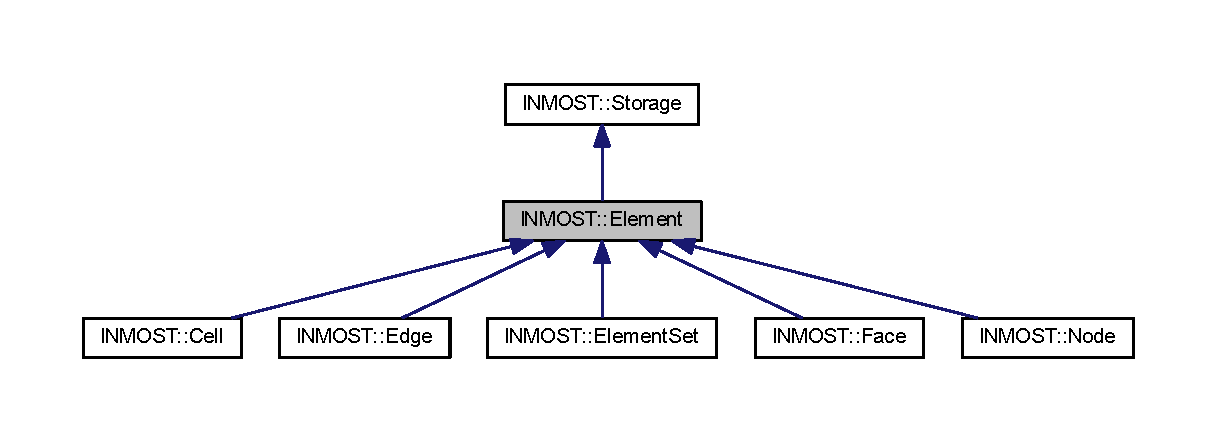
\includegraphics[width=350pt]{classINMOST_1_1Element__inherit__graph}
\end{center}
\end{figure}


Collaboration diagram for I\-N\-M\-O\-S\-T\-:\-:Element\-:\nopagebreak
\begin{figure}[H]
\begin{center}
\leavevmode
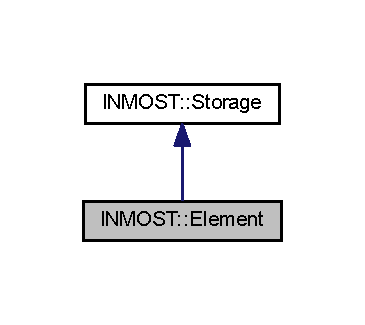
\includegraphics[width=175pt]{classINMOST_1_1Element__coll__graph}
\end{center}
\end{figure}
\subsection*{Public Types}
\begin{DoxyCompactItemize}
\item 
\hypertarget{classINMOST_1_1Element_a67ac235d4dcb5a949fa9150d5b82ebd8}{typedef I\-N\-M\-O\-S\-T\-\_\-\-D\-A\-T\-A\-\_\-\-B\-U\-L\-K\-\_\-\-T\-Y\-P\-E {\bfseries Geometric\-Type}}\label{classINMOST_1_1Element_a67ac235d4dcb5a949fa9150d5b82ebd8}

\item 
\hypertarget{classINMOST_1_1Element_ac872af2720bbc9dcf55ec63eb09c639b}{typedef I\-N\-M\-O\-S\-T\-\_\-\-D\-A\-T\-A\-\_\-\-B\-U\-L\-K\-\_\-\-T\-Y\-P\-E {\bfseries Status}}\label{classINMOST_1_1Element_ac872af2720bbc9dcf55ec63eb09c639b}

\item 
\hypertarget{classINMOST_1_1Element_aff536a514195ba59e540455bdf40fd14}{typedef inner\-\_\-reference\-\_\-array {\bfseries adj\-\_\-type}}\label{classINMOST_1_1Element_aff536a514195ba59e540455bdf40fd14}

\item 
\hypertarget{classINMOST_1_1Element_ae98d7bc1b7117dbf5ec2509138cfb610}{typedef adj\-\_\-type\-::iterator {\bfseries adj\-\_\-iterator}}\label{classINMOST_1_1Element_ae98d7bc1b7117dbf5ec2509138cfb610}

\item 
\hypertarget{classINMOST_1_1Element_a493993dcd759b29914bacee2343c099e}{typedef adj\-\_\-type\-::const\-\_\-iterator {\bfseries const\-\_\-adj\-\_\-iterator}}\label{classINMOST_1_1Element_a493993dcd759b29914bacee2343c099e}

\item 
\hypertarget{classINMOST_1_1Element_a3e3c89f0d9aa578dedb07060046da74e}{typedef adj\-\_\-type\-::reverse\-\_\-iterator {\bfseries adj\-\_\-reverse\-\_\-iterator}}\label{classINMOST_1_1Element_a3e3c89f0d9aa578dedb07060046da74e}

\item 
\hypertarget{classINMOST_1_1Element_a2212e3f149d9dab8ae5e918b9f6942ad}{typedef \\*
adj\-\_\-type\-::const\-\_\-reverse\-\_\-iterator {\bfseries const\-\_\-adj\-\_\-reverse\-\_\-iterator}}\label{classINMOST_1_1Element_a2212e3f149d9dab8ae5e918b9f6942ad}

\end{DoxyCompactItemize}
\subsection*{Public Member Functions}
\begin{DoxyCompactItemize}
\item 
\hypertarget{classINMOST_1_1Element_ad436acce5c638e2dba1092b6714d272b}{{\bfseries Element} (\hyperlink{classINMOST_1_1Mesh}{Mesh} $\ast$m, Handle\-Type h)}\label{classINMOST_1_1Element_ad436acce5c638e2dba1092b6714d272b}

\item 
\hypertarget{classINMOST_1_1Element_a479a64825cc451349225ff1a6e541d3c}{{\bfseries Element} (\hyperlink{classINMOST_1_1Mesh}{Mesh} $\ast$m, Handle\-Type $\ast$h)}\label{classINMOST_1_1Element_a479a64825cc451349225ff1a6e541d3c}

\item 
\hypertarget{classINMOST_1_1Element_a2d5ef13759950d36b16aeea99f729812}{{\bfseries Element} (const \hyperlink{classINMOST_1_1Element}{Element} \&other)}\label{classINMOST_1_1Element_a2d5ef13759950d36b16aeea99f729812}

\item 
\hypertarget{classINMOST_1_1Element_a8761a37c3bc9f46ada8f09034e8fa3a7}{\hyperlink{classINMOST_1_1Element}{Element} \& {\bfseries operator=} (\hyperlink{classINMOST_1_1Element}{Element} const \&other)}\label{classINMOST_1_1Element_a8761a37c3bc9f46ada8f09034e8fa3a7}

\item 
\hypertarget{classINMOST_1_1Element_a912fb247d1bdfbd0eb6e562a1ededd6f}{\hyperlink{classINMOST_1_1Element}{Element} $\ast$ {\bfseries operator-\/$>$} ()}\label{classINMOST_1_1Element_a912fb247d1bdfbd0eb6e562a1ededd6f}

\item 
\hypertarget{classINMOST_1_1Element_a5487af4d6ea1854a2864fae18a6932b5}{const \hyperlink{classINMOST_1_1Element}{Element} $\ast$ {\bfseries operator-\/$>$} () const }\label{classINMOST_1_1Element_a5487af4d6ea1854a2864fae18a6932b5}

\item 
\hypertarget{classINMOST_1_1Element_a2c3df3226d74ae023da7989a193acf9f}{\hyperlink{classINMOST_1_1Element}{Element} \& {\bfseries self} ()}\label{classINMOST_1_1Element_a2c3df3226d74ae023da7989a193acf9f}

\item 
\hypertarget{classINMOST_1_1Element_ab50141ec6c8da76fdd9771eed4a3c70e}{const \hyperlink{classINMOST_1_1Element}{Element} \& {\bfseries self} () const }\label{classINMOST_1_1Element_ab50141ec6c8da76fdd9771eed4a3c70e}

\item 
virtual \hyperlink{classINMOST_1_1Storage_ae333dfced6fa9cfde0c8e7dcf1b0cc2b}{enumerator} \hyperlink{classINMOST_1_1Element_a11ebdafff96a8074de4c89529f7ddf89}{nb\-Adj\-Elements} (Element\-Type etype) const 
\begin{DoxyCompactList}\small\item\em Retrieve number of adjacent elements. \end{DoxyCompactList}\item 
virtual \hyperlink{classINMOST_1_1ElementArray}{Element\-Array}$<$ \hyperlink{classINMOST_1_1Element}{Element} $>$ \hyperlink{classINMOST_1_1Element_a237d4b838a71b5bb956b70bfe65d12ca}{get\-Adj\-Elements} (Element\-Type etype) const 
\begin{DoxyCompactList}\small\item\em Retrieve unordered array of adjacent elements. \end{DoxyCompactList}\item 
virtual \hyperlink{classINMOST_1_1Storage_ae333dfced6fa9cfde0c8e7dcf1b0cc2b}{enumerator} \hyperlink{classINMOST_1_1Element_aacec7f43efcad9d16064e34854f094e4}{nb\-Adj\-Elements} (Element\-Type etype, Marker\-Type mask, bool invert\-\_\-mask=false) const 
\begin{DoxyCompactList}\small\item\em Retrieve number of adjacent elements with marker. \end{DoxyCompactList}\item 
virtual \hyperlink{classINMOST_1_1ElementArray}{Element\-Array}$<$ \hyperlink{classINMOST_1_1Element}{Element} $>$ \hyperlink{classINMOST_1_1Element_ae1b2cbfce7af2e3f38f5a19d2a9a30a1}{get\-Adj\-Elements} (Element\-Type etype, Marker\-Type mask, bool invert\-\_\-mask=false) const 
\begin{DoxyCompactList}\small\item\em Retrieve unordered array of adjacent elements with marker. \end{DoxyCompactList}\item 
\hypertarget{classINMOST_1_1Element_a57707f37922d422779109921f2b75785}{\hyperlink{classINMOST_1_1ElementArray}{Element\-Array}$<$ \hyperlink{classINMOST_1_1Element}{Element} $>$ {\bfseries Bridge\-Adjacencies} (Element\-Type Bridge, Element\-Type Dest, Marker\-Type mask=0, bool invert\-\_\-mask=false) const }\label{classINMOST_1_1Element_a57707f37922d422779109921f2b75785}

\item 
\hypertarget{classINMOST_1_1Element_a687d29f44e125a63f020f8fd87cb7f80}{\hyperlink{classINMOST_1_1ElementArray}{Element\-Array}$<$ \hyperlink{classINMOST_1_1Node}{Node} $>$ {\bfseries Bridge\-Adjacencies2\-Node} (Element\-Type Bridge, Marker\-Type mask=0, bool invert\-\_\-mask=false) const }\label{classINMOST_1_1Element_a687d29f44e125a63f020f8fd87cb7f80}

\item 
\hypertarget{classINMOST_1_1Element_aa12ffe96df6a43e20a625055898eba2c}{\hyperlink{classINMOST_1_1ElementArray}{Element\-Array}$<$ \hyperlink{classINMOST_1_1Edge}{Edge} $>$ {\bfseries Bridge\-Adjacencies2\-Edge} (Element\-Type Bridge, Marker\-Type mask=0, bool invert\-\_\-mask=false) const }\label{classINMOST_1_1Element_aa12ffe96df6a43e20a625055898eba2c}

\item 
\hypertarget{classINMOST_1_1Element_a31a0168a9eed7aa4c681e45c64b74482}{\hyperlink{classINMOST_1_1ElementArray}{Element\-Array}$<$ \hyperlink{classINMOST_1_1Face}{Face} $>$ {\bfseries Bridge\-Adjacencies2\-Face} (Element\-Type Bridge, Marker\-Type mask=0, bool invert\-\_\-mask=false) const }\label{classINMOST_1_1Element_a31a0168a9eed7aa4c681e45c64b74482}

\item 
\hypertarget{classINMOST_1_1Element_a50326950387636932804bb474cc08bce}{\hyperlink{classINMOST_1_1ElementArray}{Element\-Array}$<$ \hyperlink{classINMOST_1_1Cell}{Cell} $>$ {\bfseries Bridge\-Adjacencies2\-Cell} (Element\-Type Bridge, Marker\-Type mask=0, bool invert\-\_\-mask=false) const }\label{classINMOST_1_1Element_a50326950387636932804bb474cc08bce}

\item 
virtual \hyperlink{classINMOST_1_1ElementArray}{Element\-Array}$<$ \hyperlink{classINMOST_1_1Node}{Node} $>$ \hyperlink{classINMOST_1_1Element_a00696ff8cd77491e1c4307cae166e92d}{get\-Nodes} () const 
\begin{DoxyCompactList}\small\item\em Retrieve all the nodes of the element. \end{DoxyCompactList}\item 
virtual \hyperlink{classINMOST_1_1ElementArray}{Element\-Array}$<$ \hyperlink{classINMOST_1_1Edge}{Edge} $>$ \hyperlink{classINMOST_1_1Element_a3ba56a19eeeb283864a006b0744fac4e}{get\-Edges} () const 
\begin{DoxyCompactList}\small\item\em Retrieve all the edges of the element. \end{DoxyCompactList}\item 
virtual \hyperlink{classINMOST_1_1ElementArray}{Element\-Array}$<$ \hyperlink{classINMOST_1_1Face}{Face} $>$ \hyperlink{classINMOST_1_1Element_a2d9cc22d44f8d70c5b2876d84be6dfa5}{get\-Faces} () const 
\begin{DoxyCompactList}\small\item\em Retrieve all the faces of the element. \end{DoxyCompactList}\item 
virtual \hyperlink{classINMOST_1_1ElementArray}{Element\-Array}$<$ \hyperlink{classINMOST_1_1Cell}{Cell} $>$ \hyperlink{classINMOST_1_1Element_aa90ec6b1e297fb9c1322b5558ccb7e2d}{get\-Cells} () const 
\begin{DoxyCompactList}\small\item\em Return all the cells of the element. \end{DoxyCompactList}\item 
\hypertarget{classINMOST_1_1Element_afe6bcf4b6d9d3398151abb8dbddc333e}{virtual \hyperlink{classINMOST_1_1ElementArray}{Element\-Array}$<$ \hyperlink{classINMOST_1_1Node}{Node} $>$ {\bfseries get\-Nodes} (Marker\-Type mask, bool invert\-\_\-mask=false) const }\label{classINMOST_1_1Element_afe6bcf4b6d9d3398151abb8dbddc333e}

\item 
\hypertarget{classINMOST_1_1Element_a56a50ffdd0977523410e011e15568e52}{virtual \hyperlink{classINMOST_1_1ElementArray}{Element\-Array}$<$ \hyperlink{classINMOST_1_1Edge}{Edge} $>$ {\bfseries get\-Edges} (Marker\-Type mask, bool invert\-\_\-mask=false) const }\label{classINMOST_1_1Element_a56a50ffdd0977523410e011e15568e52}

\item 
\hypertarget{classINMOST_1_1Element_a42406f6dc1134c7daea98606c1225486}{virtual \hyperlink{classINMOST_1_1ElementArray}{Element\-Array}$<$ \hyperlink{classINMOST_1_1Face}{Face} $>$ {\bfseries get\-Faces} (Marker\-Type mask, bool invert\-\_\-mask=false) const }\label{classINMOST_1_1Element_a42406f6dc1134c7daea98606c1225486}

\item 
\hypertarget{classINMOST_1_1Element_aae8ce8b88935469fea8c4880282710a5}{virtual \hyperlink{classINMOST_1_1ElementArray}{Element\-Array}$<$ \hyperlink{classINMOST_1_1Cell}{Cell} $>$ {\bfseries get\-Cells} (Marker\-Type mask, bool invert\-\_\-mask=false) const }\label{classINMOST_1_1Element_aae8ce8b88935469fea8c4880282710a5}

\item 
\hypertarget{classINMOST_1_1Element_a9f15878b1862036517718dee27030da5}{\hyperlink{classINMOST_1_1Node}{Node} {\bfseries get\-As\-Node} () const }\label{classINMOST_1_1Element_a9f15878b1862036517718dee27030da5}

\item 
\hypertarget{classINMOST_1_1Element_a8df59b1588049676515d087a70466f3b}{\hyperlink{classINMOST_1_1Edge}{Edge} {\bfseries get\-As\-Edge} () const }\label{classINMOST_1_1Element_a8df59b1588049676515d087a70466f3b}

\item 
\hypertarget{classINMOST_1_1Element_aa8d708231a3b1da2f9006343be372bfe}{\hyperlink{classINMOST_1_1Face}{Face} {\bfseries get\-As\-Face} () const }\label{classINMOST_1_1Element_aa8d708231a3b1da2f9006343be372bfe}

\item 
\hypertarget{classINMOST_1_1Element_ae4c3af5bec31c6c9602132f6f8738265}{\hyperlink{classINMOST_1_1Cell}{Cell} {\bfseries get\-As\-Cell} () const }\label{classINMOST_1_1Element_ae4c3af5bec31c6c9602132f6f8738265}

\item 
\hypertarget{classINMOST_1_1Element_aba796c6420e3a223153683f8dd755338}{\hyperlink{classINMOST_1_1ElementSet}{Element\-Set} {\bfseries get\-As\-Set} () const }\label{classINMOST_1_1Element_aba796c6420e3a223153683f8dd755338}

\item 
\hypertarget{classINMOST_1_1Element_a26cd9c99f7dc558190a8fb4b30074d54}{Geometric\-Type {\bfseries Get\-Geometric\-Type} () const }\label{classINMOST_1_1Element_a26cd9c99f7dc558190a8fb4b30074d54}

\item 
\hypertarget{classINMOST_1_1Element_a59192ab8b9df0e7167731819023152dc}{unsigned int {\bfseries Get\-Element\-Dimension} () const }\label{classINMOST_1_1Element_a59192ab8b9df0e7167731819023152dc}

\item 
\hypertarget{classINMOST_1_1Element_a2ce199aba8ff42ec98e39feb90341283}{Status {\bfseries Get\-Status} () const }\label{classINMOST_1_1Element_a2ce199aba8ff42ec98e39feb90341283}

\item 
\hypertarget{classINMOST_1_1Element_afaae538e1103391e378efcba907aba4e}{void {\bfseries Set\-Status} (Status status) const }\label{classINMOST_1_1Element_afaae538e1103391e378efcba907aba4e}

\item 
\hypertarget{classINMOST_1_1Element_a0dd67d5686fae5c8263f7d31c9f89351}{\hyperlink{classINMOST_1_1Storage_aec96942bc647417a801e2895b45964d2}{Storage\-::integer} \& {\bfseries Global\-I\-D} () const }\label{classINMOST_1_1Element_a0dd67d5686fae5c8263f7d31c9f89351}

\item 
\hypertarget{classINMOST_1_1Element_ad03ef257847cd6ee812e60b00ec5815d}{bool {\bfseries Check\-Element\-Connectivity} () const }\label{classINMOST_1_1Element_ad03ef257847cd6ee812e60b00ec5815d}

\item 
\hypertarget{classINMOST_1_1Element_a494f4593d8a31826d05844f2cb2b58f9}{void {\bfseries Print\-Element\-Connectivity} () const }\label{classINMOST_1_1Element_a494f4593d8a31826d05844f2cb2b58f9}

\item 
\hypertarget{classINMOST_1_1Element_a1d1a89b809462f32ddb67de9fc09a28f}{void {\bfseries Cast\-Ray} (\hyperlink{classINMOST_1_1Storage_a853346784b4a5822a7fac54d8f10f805}{real} $\ast$pos, \hyperlink{classINMOST_1_1Storage_a853346784b4a5822a7fac54d8f10f805}{real} $\ast$dir, dynarray$<$ std\-::pair$<$ \hyperlink{classINMOST_1_1Element}{Element}, \hyperlink{classINMOST_1_1Storage_a853346784b4a5822a7fac54d8f10f805}{real} $>$, 16 $>$ \&hits) const }\label{classINMOST_1_1Element_a1d1a89b809462f32ddb67de9fc09a28f}

\item 
\hypertarget{classINMOST_1_1Element_ade93c392d7815a7ec6e0684b26568562}{void {\bfseries Compute\-Geometric\-Type} () const }\label{classINMOST_1_1Element_ade93c392d7815a7ec6e0684b26568562}

\item 
\hypertarget{classINMOST_1_1Element_a5e512645c1f8082d9fe401effc6deb2e}{void {\bfseries Centroid} (\hyperlink{classINMOST_1_1Storage_a853346784b4a5822a7fac54d8f10f805}{real} $\ast$cnt) const }\label{classINMOST_1_1Element_a5e512645c1f8082d9fe401effc6deb2e}

\item 
\hypertarget{classINMOST_1_1Element_a006a4b60505738c328560656a4279b53}{void {\bfseries Barycenter} (\hyperlink{classINMOST_1_1Storage_a853346784b4a5822a7fac54d8f10f805}{real} $\ast$cnt) const }\label{classINMOST_1_1Element_a006a4b60505738c328560656a4279b53}

\item 
\hypertarget{classINMOST_1_1Element_a0409db870d0ac2787f10f4e16ccfd5b9}{\hyperlink{classINMOST_1_1Storage_a853346784b4a5822a7fac54d8f10f805}{Storage\-::real} {\bfseries Mean} (\hyperlink{classINMOST_1_1Storage_a853346784b4a5822a7fac54d8f10f805}{real}($\ast$func)(\hyperlink{classINMOST_1_1Storage_a853346784b4a5822a7fac54d8f10f805}{real} $\ast$x, \hyperlink{classINMOST_1_1Storage_a853346784b4a5822a7fac54d8f10f805}{real} t), \hyperlink{classINMOST_1_1Storage_a853346784b4a5822a7fac54d8f10f805}{real} time) const }\label{classINMOST_1_1Element_a0409db870d0ac2787f10f4e16ccfd5b9}

\item 
\hypertarget{classINMOST_1_1Element_a1549d3353773bc9a020fd4e196520fbc}{bool {\bfseries Boundary} () const }\label{classINMOST_1_1Element_a1549d3353773bc9a020fd4e196520fbc}

\item 
\hypertarget{classINMOST_1_1Element_aa7881c66a2afd84eaa0089e62230bc39}{bool {\bfseries Planarity} () const }\label{classINMOST_1_1Element_aa7881c66a2afd84eaa0089e62230bc39}

\item 
\hypertarget{classINMOST_1_1Element_a2a6833f66a162e7684c33871d196c3fe}{bool {\bfseries Hide} () const }\label{classINMOST_1_1Element_a2a6833f66a162e7684c33871d196c3fe}

\item 
\hypertarget{classINMOST_1_1Element_a9b00fa9fb06ad1e1f88b17aa8d26d168}{bool {\bfseries Show} () const }\label{classINMOST_1_1Element_a9b00fa9fb06ad1e1f88b17aa8d26d168}

\item 
\hypertarget{classINMOST_1_1Element_ab07dd77f97d0c81c90b62cdcecdcf2a9}{bool {\bfseries Delete} ()}\label{classINMOST_1_1Element_ab07dd77f97d0c81c90b62cdcecdcf2a9}

\item 
\hypertarget{classINMOST_1_1Element_a47104b37b08a694ec9da21a4e0a158eb}{bool {\bfseries Hidden} () const }\label{classINMOST_1_1Element_a47104b37b08a694ec9da21a4e0a158eb}

\item 
\hypertarget{classINMOST_1_1Element_ad4f1593d17c29484b3b6d72cc17a76ba}{bool {\bfseries New} () const }\label{classINMOST_1_1Element_ad4f1593d17c29484b3b6d72cc17a76ba}

\item 
\hypertarget{classINMOST_1_1Element_a1472c6e7f2e52366dedba12c6138bc17}{void {\bfseries Disconnect} (bool delete\-\_\-upper\-\_\-adjacent) const }\label{classINMOST_1_1Element_a1472c6e7f2e52366dedba12c6138bc17}

\item 
void \hyperlink{classINMOST_1_1Element_a1fdc3e5b00005d5831bb62222823a737}{Disconnect} (const Handle\-Type $\ast$adjacent, I\-N\-M\-O\-S\-T\-\_\-\-D\-A\-T\-A\-\_\-\-E\-N\-U\-M\-\_\-\-T\-Y\-P\-E num) const 
\begin{DoxyCompactList}\small\item\em Disconnect element. \end{DoxyCompactList}\item 
void \hyperlink{classINMOST_1_1Element_a96bd136b0f249c958fc8632553aa3b58}{Connect} (const Handle\-Type $\ast$adjacent, I\-N\-M\-O\-S\-T\-\_\-\-D\-A\-T\-A\-\_\-\-E\-N\-U\-M\-\_\-\-T\-Y\-P\-E num) const 
\begin{DoxyCompactList}\small\item\em Connects lower adjacencies to current element. \end{DoxyCompactList}\item 
\hypertarget{classINMOST_1_1Element_ad226d6f51de0ee33111fa2d9ee77e2ce}{void \hyperlink{classINMOST_1_1Element_ad226d6f51de0ee33111fa2d9ee77e2ce}{Update\-Geometric\-Data} () const }\label{classINMOST_1_1Element_ad226d6f51de0ee33111fa2d9ee77e2ce}

\begin{DoxyCompactList}\small\item\em Update geometric data for element, calls Recompute\-Geometric\-Data from \hyperlink{classINMOST_1_1Mesh}{Mesh}. \end{DoxyCompactList}\end{DoxyCompactItemize}
\subsection*{Static Public Member Functions}
\begin{DoxyCompactItemize}
\item 
\hypertarget{classINMOST_1_1Element_a0a1993360a4b2767e808db24905f660c}{static const char $\ast$ {\bfseries Geometric\-Type\-Name} (Geometric\-Type t)}\label{classINMOST_1_1Element_a0a1993360a4b2767e808db24905f660c}

\item 
\hypertarget{classINMOST_1_1Element_a68fb90367eb06a63b69bb3059733d110}{static \hyperlink{classINMOST_1_1Storage_aec96942bc647417a801e2895b45964d2}{integer} {\bfseries Get\-Geometric\-Dimension} (Geometric\-Type m\-\_\-type)}\label{classINMOST_1_1Element_a68fb90367eb06a63b69bb3059733d110}

\item 
\hypertarget{classINMOST_1_1Element_a6d81cab77a57f33fb614505c21767841}{static const char $\ast$ {\bfseries Status\-Name} (Status s)}\label{classINMOST_1_1Element_a6d81cab77a57f33fb614505c21767841}

\item 
\hypertarget{classINMOST_1_1Element_acedd520621e7c5da55d1b17ccb671aa8}{static bool {\bfseries Check\-Connectivity} (\hyperlink{classINMOST_1_1Mesh}{Mesh} $\ast$m)}\label{classINMOST_1_1Element_acedd520621e7c5da55d1b17ccb671aa8}

\end{DoxyCompactItemize}
\subsection*{Static Public Attributes}
\begin{DoxyCompactItemize}
\item 
\hypertarget{classINMOST_1_1Element_a5786982660a3e36c8737bfe21b82f97e}{static const Geometric\-Type {\bfseries Unset} = 0}\label{classINMOST_1_1Element_a5786982660a3e36c8737bfe21b82f97e}

\item 
\hypertarget{classINMOST_1_1Element_ad950b353be0244125d5357f129ba88b1}{static const Geometric\-Type {\bfseries Vertex} = 1}\label{classINMOST_1_1Element_ad950b353be0244125d5357f129ba88b1}

\item 
\hypertarget{classINMOST_1_1Element_aa72c7c2cc44eec2d75ba542d7decd69e}{static const Geometric\-Type {\bfseries Line} = 2}\label{classINMOST_1_1Element_aa72c7c2cc44eec2d75ba542d7decd69e}

\item 
\hypertarget{classINMOST_1_1Element_ad48b58c89bb22135c5a6df5e7bb5e17a}{static const Geometric\-Type {\bfseries Multi\-Line} = 3}\label{classINMOST_1_1Element_ad48b58c89bb22135c5a6df5e7bb5e17a}

\item 
\hypertarget{classINMOST_1_1Element_a59e88a5983029f92558294c29b7ca2d0}{static const Geometric\-Type {\bfseries Tri} = 4}\label{classINMOST_1_1Element_a59e88a5983029f92558294c29b7ca2d0}

\item 
\hypertarget{classINMOST_1_1Element_a051ce85c1ea896e08463c8598d69c705}{static const Geometric\-Type {\bfseries Quad} = 5}\label{classINMOST_1_1Element_a051ce85c1ea896e08463c8598d69c705}

\item 
\hypertarget{classINMOST_1_1Element_a95ee00f2fb07adb32080be429aea53fd}{static const Geometric\-Type {\bfseries Polygon} = 6}\label{classINMOST_1_1Element_a95ee00f2fb07adb32080be429aea53fd}

\item 
\hypertarget{classINMOST_1_1Element_a7f22e034805676dc0529248255ead16a}{static const Geometric\-Type {\bfseries Multi\-Polygon} = 7}\label{classINMOST_1_1Element_a7f22e034805676dc0529248255ead16a}

\item 
\hypertarget{classINMOST_1_1Element_a83f9fdad8c678146cb5e6cbf6aee94d1}{static const Geometric\-Type {\bfseries Tet} = 8}\label{classINMOST_1_1Element_a83f9fdad8c678146cb5e6cbf6aee94d1}

\item 
\hypertarget{classINMOST_1_1Element_aa118032da38a237b4bfe999bcea30616}{static const Geometric\-Type {\bfseries Hex} = 9}\label{classINMOST_1_1Element_aa118032da38a237b4bfe999bcea30616}

\item 
\hypertarget{classINMOST_1_1Element_a1c5357c5bc37b9a18448f45b2999ff93}{static const Geometric\-Type {\bfseries Prism} = 10}\label{classINMOST_1_1Element_a1c5357c5bc37b9a18448f45b2999ff93}

\item 
\hypertarget{classINMOST_1_1Element_a7be746df43ae83225c179d9c09205904}{static const Geometric\-Type {\bfseries Pyramid} = 11}\label{classINMOST_1_1Element_a7be746df43ae83225c179d9c09205904}

\item 
\hypertarget{classINMOST_1_1Element_a03a7256f661e0a0a5ff9008a694370d4}{static const Geometric\-Type {\bfseries Polyhedron} = 12}\label{classINMOST_1_1Element_a03a7256f661e0a0a5ff9008a694370d4}

\item 
\hypertarget{classINMOST_1_1Element_abd644aef30cb508b45f7936b8e5a6e82}{static const Geometric\-Type {\bfseries Set} = 253}\label{classINMOST_1_1Element_abd644aef30cb508b45f7936b8e5a6e82}

\item 
\hypertarget{classINMOST_1_1Element_a21768dc12b1f404d41952d8b82e46763}{static const Geometric\-Type {\bfseries Mesh\-Part} = 254}\label{classINMOST_1_1Element_a21768dc12b1f404d41952d8b82e46763}

\item 
\hypertarget{classINMOST_1_1Element_aeb3304586912f10eaa2a40f6b5b610ba}{static const Geometric\-Type {\bfseries Max\-Type} = 255}\label{classINMOST_1_1Element_aeb3304586912f10eaa2a40f6b5b610ba}

\item 
\hypertarget{classINMOST_1_1Element_a3a907402d1e52df299d3fc6db6d92e56}{static const Status {\bfseries Owned} = 1}\label{classINMOST_1_1Element_a3a907402d1e52df299d3fc6db6d92e56}

\item 
\hypertarget{classINMOST_1_1Element_a0251c6ad6407192d9a41b7ad3587bfdb}{static const Status {\bfseries Shared} = 2}\label{classINMOST_1_1Element_a0251c6ad6407192d9a41b7ad3587bfdb}

\item 
\hypertarget{classINMOST_1_1Element_a109dae89d1d8e4d76078f6e4498d58b5}{static const Status {\bfseries Ghost} = 4}\label{classINMOST_1_1Element_a109dae89d1d8e4d76078f6e4498d58b5}

\item 
\hypertarget{classINMOST_1_1Element_ad7f0b488fca1d2f2a832345c77f83760}{static const Status {\bfseries Any} = 0}\label{classINMOST_1_1Element_ad7f0b488fca1d2f2a832345c77f83760}

\end{DoxyCompactItemize}
\subsection*{Protected Member Functions}
\begin{DoxyCompactItemize}
\item 
\hypertarget{classINMOST_1_1Element_a594740fbcce07e274b4cd6115073188f}{void {\bfseries Set\-Geometric\-Type} (Geometric\-Type t)}\label{classINMOST_1_1Element_a594740fbcce07e274b4cd6115073188f}

\end{DoxyCompactItemize}
\subsection*{Additional Inherited Members}


\subsection{Member Function Documentation}
\hypertarget{classINMOST_1_1Element_a96bd136b0f249c958fc8632553aa3b58}{\index{I\-N\-M\-O\-S\-T\-::\-Element@{I\-N\-M\-O\-S\-T\-::\-Element}!Connect@{Connect}}
\index{Connect@{Connect}!INMOST::Element@{I\-N\-M\-O\-S\-T\-::\-Element}}
\subsubsection[{Connect}]{\setlength{\rightskip}{0pt plus 5cm}void I\-N\-M\-O\-S\-T\-::\-Element\-::\-Connect (
\begin{DoxyParamCaption}
\item[{const Handle\-Type $\ast$}]{adjacent, }
\item[{I\-N\-M\-O\-S\-T\-\_\-\-D\-A\-T\-A\-\_\-\-E\-N\-U\-M\-\_\-\-T\-Y\-P\-E}]{num}
\end{DoxyParamCaption}
) const}}\label{classINMOST_1_1Element_a96bd136b0f249c958fc8632553aa3b58}


Connects lower adjacencies to current element. 

Geometric data and cell nodes are updated automatically.

\begin{DoxyRefDesc}{Todo}
\item[\hyperlink{todo__todo000001}{Todo}]
\begin{DoxyEnumerate}
\item Asserts in this function should be replaced by Topography checks.
\item This function should be used for construction of elements instead of current implementation.
\item Should correctly account for order of edges (may be implemented through Check\-Edge\-Order, Fix\-Edge\-Order). 
\end{DoxyEnumerate}\end{DoxyRefDesc}
\hypertarget{classINMOST_1_1Element_a1fdc3e5b00005d5831bb62222823a737}{\index{I\-N\-M\-O\-S\-T\-::\-Element@{I\-N\-M\-O\-S\-T\-::\-Element}!Disconnect@{Disconnect}}
\index{Disconnect@{Disconnect}!INMOST::Element@{I\-N\-M\-O\-S\-T\-::\-Element}}
\subsubsection[{Disconnect}]{\setlength{\rightskip}{0pt plus 5cm}void I\-N\-M\-O\-S\-T\-::\-Element\-::\-Disconnect (
\begin{DoxyParamCaption}
\item[{const Handle\-Type $\ast$}]{adjacent, }
\item[{I\-N\-M\-O\-S\-T\-\_\-\-D\-A\-T\-A\-\_\-\-E\-N\-U\-M\-\_\-\-T\-Y\-P\-E}]{num}
\end{DoxyParamCaption}
) const}}\label{classINMOST_1_1Element_a1fdc3e5b00005d5831bb62222823a737}


Disconnect element. 

Disconnects nodes from this edge, edges from this face, faces from this cell, cannot disconnect cells from this node; \par
Disconnects edges from this node, faces from this edge, cells from this face, cannot disconnect nodes from this cell; \par
Updates geometric data and cell nodes automatically. \hypertarget{classINMOST_1_1Element_a237d4b838a71b5bb956b70bfe65d12ca}{\index{I\-N\-M\-O\-S\-T\-::\-Element@{I\-N\-M\-O\-S\-T\-::\-Element}!get\-Adj\-Elements@{get\-Adj\-Elements}}
\index{get\-Adj\-Elements@{get\-Adj\-Elements}!INMOST::Element@{I\-N\-M\-O\-S\-T\-::\-Element}}
\subsubsection[{get\-Adj\-Elements}]{\setlength{\rightskip}{0pt plus 5cm}virtual {\bf Element\-Array}$<${\bf Element}$>$ I\-N\-M\-O\-S\-T\-::\-Element\-::get\-Adj\-Elements (
\begin{DoxyParamCaption}
\item[{Element\-Type}]{etype}
\end{DoxyParamCaption}
) const\hspace{0.3cm}{\ttfamily [virtual]}}}\label{classINMOST_1_1Element_a237d4b838a71b5bb956b70bfe65d12ca}


Retrieve unordered array of adjacent elements. 

If you care about orderness of nodes for face you should you \hyperlink{classINMOST_1_1Face_a102ef5504795e2b3607093071259397e}{Face\-::get\-Nodes()} instead. If you want faster access you may use direct access to handles stored in memory through \hyperlink{classINMOST_1_1Mesh_a1e7462d775868bb6ef687cef8a5198cb}{Mesh\-::\-High\-Conn} for upper adjacencies and \hyperlink{classINMOST_1_1Mesh_ad20f64a301adf9c3fafe28a8f921a791}{Mesh\-::\-Low\-Conn} for lower adjacencies. 
\begin{DoxyParams}{Parameters}
{\em etype} & bitwise mask of element types \\
\hline
\end{DoxyParams}
\begin{DoxyReturn}{Returns}
array of elements 
\end{DoxyReturn}


Reimplemented in \hyperlink{classINMOST_1_1ElementSet_a7ade4a7bc7ac22b929738d7bf75e3144}{I\-N\-M\-O\-S\-T\-::\-Element\-Set}.

\hypertarget{classINMOST_1_1Element_ae1b2cbfce7af2e3f38f5a19d2a9a30a1}{\index{I\-N\-M\-O\-S\-T\-::\-Element@{I\-N\-M\-O\-S\-T\-::\-Element}!get\-Adj\-Elements@{get\-Adj\-Elements}}
\index{get\-Adj\-Elements@{get\-Adj\-Elements}!INMOST::Element@{I\-N\-M\-O\-S\-T\-::\-Element}}
\subsubsection[{get\-Adj\-Elements}]{\setlength{\rightskip}{0pt plus 5cm}virtual {\bf Element\-Array}$<${\bf Element}$>$ I\-N\-M\-O\-S\-T\-::\-Element\-::get\-Adj\-Elements (
\begin{DoxyParamCaption}
\item[{Element\-Type}]{etype, }
\item[{Marker\-Type}]{mask, }
\item[{bool}]{invert\-\_\-mask = {\ttfamily false}}
\end{DoxyParamCaption}
) const\hspace{0.3cm}{\ttfamily [virtual]}}}\label{classINMOST_1_1Element_ae1b2cbfce7af2e3f38f5a19d2a9a30a1}


Retrieve unordered array of adjacent elements with marker. 


\begin{DoxyParams}{Parameters}
{\em etype} & bitwise mask of element types \\
\hline
{\em mask} & marker to be set \\
\hline
{\em invert\-\_\-mask} & if true then those are selected on wich marker is not set \\
\hline
\end{DoxyParams}
\begin{DoxyReturn}{Returns}
array of elements 
\end{DoxyReturn}


Reimplemented in \hyperlink{classINMOST_1_1ElementSet_aec40c76a04a0180105fcdddedb31da63}{I\-N\-M\-O\-S\-T\-::\-Element\-Set}.

\hypertarget{classINMOST_1_1Element_aa90ec6b1e297fb9c1322b5558ccb7e2d}{\index{I\-N\-M\-O\-S\-T\-::\-Element@{I\-N\-M\-O\-S\-T\-::\-Element}!get\-Cells@{get\-Cells}}
\index{get\-Cells@{get\-Cells}!INMOST::Element@{I\-N\-M\-O\-S\-T\-::\-Element}}
\subsubsection[{get\-Cells}]{\setlength{\rightskip}{0pt plus 5cm}virtual {\bf Element\-Array}$<${\bf Cell}$>$ I\-N\-M\-O\-S\-T\-::\-Element\-::get\-Cells (
\begin{DoxyParamCaption}
{}
\end{DoxyParamCaption}
) const\hspace{0.3cm}{\ttfamily [virtual]}}}\label{classINMOST_1_1Element_aa90ec6b1e297fb9c1322b5558ccb7e2d}


Return all the cells of the element. 

For a node returns unordered set of cells.

For an edge returns unordered set of cells.

For a face returns a pair of cells. In the case Face\-::\-Check\-Normal\-Orientation returns true then the normal points from the first cell to the second and in oppisite direction otherwise.

For a cell returns itself.

\begin{DoxyReturn}{Returns}
array of elements 
\end{DoxyReturn}
\begin{DoxySeeAlso}{See Also}
Face\-::\-Face\-Oriented\-Outside 
\end{DoxySeeAlso}


Reimplemented in \hyperlink{classINMOST_1_1ElementSet_a1ac9b271c2ddf7ea193c1f2711f59df4}{I\-N\-M\-O\-S\-T\-::\-Element\-Set}, \hyperlink{classINMOST_1_1Face_a4c1a9d6300f0b8da3032753380a1846c}{I\-N\-M\-O\-S\-T\-::\-Face}, \hyperlink{classINMOST_1_1Edge_ab38cdf43f623abcc12b0befbfac27b90}{I\-N\-M\-O\-S\-T\-::\-Edge}, and \hyperlink{classINMOST_1_1Node_a50abc7d16b296a9f6a2e1211dfb1d35a}{I\-N\-M\-O\-S\-T\-::\-Node}.

\hypertarget{classINMOST_1_1Element_a3ba56a19eeeb283864a006b0744fac4e}{\index{I\-N\-M\-O\-S\-T\-::\-Element@{I\-N\-M\-O\-S\-T\-::\-Element}!get\-Edges@{get\-Edges}}
\index{get\-Edges@{get\-Edges}!INMOST::Element@{I\-N\-M\-O\-S\-T\-::\-Element}}
\subsubsection[{get\-Edges}]{\setlength{\rightskip}{0pt plus 5cm}virtual {\bf Element\-Array}$<${\bf Edge}$>$ I\-N\-M\-O\-S\-T\-::\-Element\-::get\-Edges (
\begin{DoxyParamCaption}
{}
\end{DoxyParamCaption}
) const\hspace{0.3cm}{\ttfamily [virtual]}}}\label{classINMOST_1_1Element_a3ba56a19eeeb283864a006b0744fac4e}


Retrieve all the edges of the element. 

For a node returns unordered set of edges.

For an edge returns itself.

For a face returns ordered set of edges.

For a cell returns unordered set of edges.

\begin{DoxyReturn}{Returns}
array of elements 
\end{DoxyReturn}


Reimplemented in \hyperlink{classINMOST_1_1ElementSet_a89ac64c67135a46eed6475b84fe330a8}{I\-N\-M\-O\-S\-T\-::\-Element\-Set}, \hyperlink{classINMOST_1_1Cell_ab0f9c4743826338a4df1b61b69b37c40}{I\-N\-M\-O\-S\-T\-::\-Cell}, \hyperlink{classINMOST_1_1Face_aaf5b6793bec15dec905f198b2c46c912}{I\-N\-M\-O\-S\-T\-::\-Face}, and \hyperlink{classINMOST_1_1Node_a43ca7289620b6df3347a1d5622350edb}{I\-N\-M\-O\-S\-T\-::\-Node}.

\hypertarget{classINMOST_1_1Element_a2d9cc22d44f8d70c5b2876d84be6dfa5}{\index{I\-N\-M\-O\-S\-T\-::\-Element@{I\-N\-M\-O\-S\-T\-::\-Element}!get\-Faces@{get\-Faces}}
\index{get\-Faces@{get\-Faces}!INMOST::Element@{I\-N\-M\-O\-S\-T\-::\-Element}}
\subsubsection[{get\-Faces}]{\setlength{\rightskip}{0pt plus 5cm}virtual {\bf Element\-Array}$<${\bf Face}$>$ I\-N\-M\-O\-S\-T\-::\-Element\-::get\-Faces (
\begin{DoxyParamCaption}
{}
\end{DoxyParamCaption}
) const\hspace{0.3cm}{\ttfamily [virtual]}}}\label{classINMOST_1_1Element_a2d9cc22d44f8d70c5b2876d84be6dfa5}


Retrieve all the faces of the element. 

For a node returns unordered set of faces.

For an edge returns unordered set of faces.

For a face returns itself.

For a cell return ordered set of faces. The order of faces in the cell is preserved from the first construction.

\begin{DoxyReturn}{Returns}
array of elements 
\end{DoxyReturn}


Reimplemented in \hyperlink{classINMOST_1_1ElementSet_a7b0d595c190a82196b2bbff022ef46eb}{I\-N\-M\-O\-S\-T\-::\-Element\-Set}, \hyperlink{classINMOST_1_1Cell_a85ccc42adbb161a36a866fcea0f961d2}{I\-N\-M\-O\-S\-T\-::\-Cell}, \hyperlink{classINMOST_1_1Edge_abfe4ce06477cfa404306c716d026d2ed}{I\-N\-M\-O\-S\-T\-::\-Edge}, and \hyperlink{classINMOST_1_1Node_a75d85d68fcd08f7d7f54a14d017bfbe2}{I\-N\-M\-O\-S\-T\-::\-Node}.

\hypertarget{classINMOST_1_1Element_a00696ff8cd77491e1c4307cae166e92d}{\index{I\-N\-M\-O\-S\-T\-::\-Element@{I\-N\-M\-O\-S\-T\-::\-Element}!get\-Nodes@{get\-Nodes}}
\index{get\-Nodes@{get\-Nodes}!INMOST::Element@{I\-N\-M\-O\-S\-T\-::\-Element}}
\subsubsection[{get\-Nodes}]{\setlength{\rightskip}{0pt plus 5cm}virtual {\bf Element\-Array}$<${\bf Node}$>$ I\-N\-M\-O\-S\-T\-::\-Element\-::get\-Nodes (
\begin{DoxyParamCaption}
{}
\end{DoxyParamCaption}
) const\hspace{0.3cm}{\ttfamily [virtual]}}}\label{classINMOST_1_1Element_a00696ff8cd77491e1c4307cae166e92d}


Retrieve all the nodes of the element. 

For a node returns itself.

For an edge returns ordered pair of nodes. The order of nodes in the edge is preserved from the first construction.

For a face returns ordered set of nodes. In the case Face\-::\-Check\-Normal\-Orientation returns true the order of nodes will follow right hand side rule with respect to normal vector, otherwise it follows left hand side rule with respect to normal vector.

For a cell returns the same order that was provided through suggest\-\_\-nodes\-\_\-oreder in Mesh\-::\-Create\-Cell. In the case suggest\-\_\-nodes\-\_\-order was not provided, the order of nodes follows V\-T\-K format for known types of elements such as Element\-::\-Tet, Element\-::\-Prism, Element\-::\-Hex, Element\-::\-Pyramid. For a general polyhedron the order is unspecified.

\begin{DoxyReturn}{Returns}
array of elements 
\end{DoxyReturn}
\begin{DoxySeeAlso}{See Also}
Face\-::\-Check\-Normal\-Orientation 

Face\-::\-Face\-Oriented\-Outside 
\end{DoxySeeAlso}


Reimplemented in \hyperlink{classINMOST_1_1ElementSet_a189d152060b36e7800c08e7d0f94fdfa}{I\-N\-M\-O\-S\-T\-::\-Element\-Set}, \hyperlink{classINMOST_1_1Cell_acc265095375df199a083a344d56e4645}{I\-N\-M\-O\-S\-T\-::\-Cell}, \hyperlink{classINMOST_1_1Face_a102ef5504795e2b3607093071259397e}{I\-N\-M\-O\-S\-T\-::\-Face}, and \hyperlink{classINMOST_1_1Edge_a2e9e02817c50da41d366d9d89ff45bb8}{I\-N\-M\-O\-S\-T\-::\-Edge}.

\hypertarget{classINMOST_1_1Element_a11ebdafff96a8074de4c89529f7ddf89}{\index{I\-N\-M\-O\-S\-T\-::\-Element@{I\-N\-M\-O\-S\-T\-::\-Element}!nb\-Adj\-Elements@{nb\-Adj\-Elements}}
\index{nb\-Adj\-Elements@{nb\-Adj\-Elements}!INMOST::Element@{I\-N\-M\-O\-S\-T\-::\-Element}}
\subsubsection[{nb\-Adj\-Elements}]{\setlength{\rightskip}{0pt plus 5cm}virtual {\bf enumerator} I\-N\-M\-O\-S\-T\-::\-Element\-::nb\-Adj\-Elements (
\begin{DoxyParamCaption}
\item[{Element\-Type}]{etype}
\end{DoxyParamCaption}
) const\hspace{0.3cm}{\ttfamily [virtual]}}}\label{classINMOST_1_1Element_a11ebdafff96a8074de4c89529f7ddf89}


Retrieve number of adjacent elements. 

For etype you can either pass one type as C\-E\-L\-L, or several types as bitwise mask\-: N\-O\-D\-E $|$ C\-E\-L\-L. 
\begin{DoxyParams}{Parameters}
{\em etype} & bitwise mask of element types \\
\hline
\end{DoxyParams}
\begin{DoxyReturn}{Returns}
number of adjacent elements. 
\end{DoxyReturn}


Reimplemented in \hyperlink{classINMOST_1_1ElementSet_a47eeee88d1c207c2cef615721013d102}{I\-N\-M\-O\-S\-T\-::\-Element\-Set}.

\hypertarget{classINMOST_1_1Element_aacec7f43efcad9d16064e34854f094e4}{\index{I\-N\-M\-O\-S\-T\-::\-Element@{I\-N\-M\-O\-S\-T\-::\-Element}!nb\-Adj\-Elements@{nb\-Adj\-Elements}}
\index{nb\-Adj\-Elements@{nb\-Adj\-Elements}!INMOST::Element@{I\-N\-M\-O\-S\-T\-::\-Element}}
\subsubsection[{nb\-Adj\-Elements}]{\setlength{\rightskip}{0pt plus 5cm}virtual {\bf enumerator} I\-N\-M\-O\-S\-T\-::\-Element\-::nb\-Adj\-Elements (
\begin{DoxyParamCaption}
\item[{Element\-Type}]{etype, }
\item[{Marker\-Type}]{mask, }
\item[{bool}]{invert\-\_\-mask = {\ttfamily false}}
\end{DoxyParamCaption}
) const\hspace{0.3cm}{\ttfamily [virtual]}}}\label{classINMOST_1_1Element_aacec7f43efcad9d16064e34854f094e4}


Retrieve number of adjacent elements with marker. 

As etype you can either pass one type as C\-E\-L\-L, or several types as bitwise mask\-: N\-O\-D\-E $|$ C\-E\-L\-L 
\begin{DoxyParams}{Parameters}
{\em etype} & bitwise mask of element types \\
\hline
{\em mask} & marker to be set \\
\hline
{\em invert\-\_\-mask} & if true then those are selected on wich marker is not set \\
\hline
\end{DoxyParams}
\begin{DoxyReturn}{Returns}
number of adjacent elements. 
\end{DoxyReturn}


Reimplemented in \hyperlink{classINMOST_1_1ElementSet_a4d3408a6908095a029584c24701e1144}{I\-N\-M\-O\-S\-T\-::\-Element\-Set}.



The documentation for this class was generated from the following file\-:\begin{DoxyCompactItemize}
\item 
inmost\-\_\-mesh.\-h\end{DoxyCompactItemize}

\hypertarget{classINMOST_1_1ElementArray}{\section{I\-N\-M\-O\-S\-T\-:\-:Element\-Array$<$ Storage\-Type $>$ Class Template Reference}
\label{classINMOST_1_1ElementArray}\index{I\-N\-M\-O\-S\-T\-::\-Element\-Array$<$ Storage\-Type $>$@{I\-N\-M\-O\-S\-T\-::\-Element\-Array$<$ Storage\-Type $>$}}
}
\subsection*{Classes}
\begin{DoxyCompactItemize}
\item 
class \hyperlink{classINMOST_1_1ElementArray_1_1const__iterator}{const\-\_\-iterator}
\item 
class \hyperlink{classINMOST_1_1ElementArray_1_1const__reverse__iterator}{const\-\_\-reverse\-\_\-iterator}
\item 
class \hyperlink{classINMOST_1_1ElementArray_1_1iterator}{iterator}
\item 
class \hyperlink{classINMOST_1_1ElementArray_1_1reverse__iterator}{reverse\-\_\-iterator}
\end{DoxyCompactItemize}
\subsection*{Public Types}
\begin{DoxyCompactItemize}
\item 
\hypertarget{classINMOST_1_1ElementArray_a0eae35b4911aae7e9e795bc4896e3610}{typedef dynarray$<$ Handle\-Type, 64 $>$ {\bfseries cont\-\_\-t}}\label{classINMOST_1_1ElementArray_a0eae35b4911aae7e9e795bc4896e3610}

\item 
\hypertarget{classINMOST_1_1ElementArray_ab9db6ec4d56669d2b45b04e5023655dd}{typedef cont\-\_\-t\-::size\-\_\-type {\bfseries size\-\_\-type}}\label{classINMOST_1_1ElementArray_ab9db6ec4d56669d2b45b04e5023655dd}

\end{DoxyCompactItemize}
\subsection*{Public Member Functions}
\begin{DoxyCompactItemize}
\item 
\hypertarget{classINMOST_1_1ElementArray_ae7800245fe85174f74b7663f142ce924}{const cont\-\_\-t \& {\bfseries Get\-Container} ()}\label{classINMOST_1_1ElementArray_ae7800245fe85174f74b7663f142ce924}

\item 
\hypertarget{classINMOST_1_1ElementArray_aae95f7c16f9abb5a846d0ab505cd96bd}{{\bfseries Element\-Array} (\hyperlink{classINMOST_1_1Mesh}{Mesh} $\ast$m\-\_\-link)}\label{classINMOST_1_1ElementArray_aae95f7c16f9abb5a846d0ab505cd96bd}

\item 
\hypertarget{classINMOST_1_1ElementArray_ab524156c027e8dd9bc1fcc1863539bc2}{{\bfseries Element\-Array} (\hyperlink{classINMOST_1_1Mesh}{Mesh} $\ast$m\-\_\-link, size\-\_\-type n, Handle\-Type h=Invalid\-Handle())}\label{classINMOST_1_1ElementArray_ab524156c027e8dd9bc1fcc1863539bc2}

\item 
\hypertarget{classINMOST_1_1ElementArray_a5d472c64c7292b1f0d5d11a2f7a9c986}{{\bfseries Element\-Array} (\hyperlink{classINMOST_1_1Mesh}{Mesh} $\ast$m\-\_\-link, const cont\-\_\-t \&c)}\label{classINMOST_1_1ElementArray_a5d472c64c7292b1f0d5d11a2f7a9c986}

\item 
\hypertarget{classINMOST_1_1ElementArray_a4a4fa5f1fb61b8f0bc5d28d5004235d5}{{\bfseries Element\-Array} (const \hyperlink{classINMOST_1_1ElementArray}{Element\-Array} \&other)}\label{classINMOST_1_1ElementArray_a4a4fa5f1fb61b8f0bc5d28d5004235d5}

\item 
\hypertarget{classINMOST_1_1ElementArray_a989a65d8b61736d0e8785977243670dc}{{\footnotesize template$<$class Input\-Iterator $>$ }\\{\bfseries Element\-Array} (\hyperlink{classINMOST_1_1Mesh}{Mesh} $\ast$m\-\_\-link, Input\-Iterator first, Input\-Iterator last)}\label{classINMOST_1_1ElementArray_a989a65d8b61736d0e8785977243670dc}

\item 
\hypertarget{classINMOST_1_1ElementArray_af53c7ec0f355c3040d01f70071202491}{\hyperlink{classINMOST_1_1ElementArray}{Element\-Array} \& {\bfseries operator=} (\hyperlink{classINMOST_1_1ElementArray}{Element\-Array} const \&other)}\label{classINMOST_1_1ElementArray_af53c7ec0f355c3040d01f70071202491}

\item 
\hypertarget{classINMOST_1_1ElementArray_ad32963d8a104222558f6204d991a38a9}{{\footnotesize template$<$class Input\-Iterator $>$ }\\\-\_\-\-\_\-\-I\-N\-L\-I\-N\-E void {\bfseries insert} (\hyperlink{classINMOST_1_1ElementArray_1_1iterator}{iterator} pos, Input\-Iterator pbeg, Input\-Iterator pend)}\label{classINMOST_1_1ElementArray_ad32963d8a104222558f6204d991a38a9}

\item 
\hypertarget{classINMOST_1_1ElementArray_a52337d2ab362cc95b0df62c516ef4161}{\-\_\-\-\_\-\-I\-N\-L\-I\-N\-E \hyperlink{classINMOST_1_1ElementArray_1_1iterator}{iterator} {\bfseries erase} (\hyperlink{classINMOST_1_1ElementArray_1_1iterator}{iterator} pos)}\label{classINMOST_1_1ElementArray_a52337d2ab362cc95b0df62c516ef4161}

\item 
\hypertarget{classINMOST_1_1ElementArray_ad359cc57cc4876553c7e993f028bc401}{\-\_\-\-\_\-\-I\-N\-L\-I\-N\-E \hyperlink{classINMOST_1_1ElementArray_1_1iterator}{iterator} {\bfseries begin} ()}\label{classINMOST_1_1ElementArray_ad359cc57cc4876553c7e993f028bc401}

\item 
\hypertarget{classINMOST_1_1ElementArray_a0944bdd27c959a51d37e20987f208e84}{\-\_\-\-\_\-\-I\-N\-L\-I\-N\-E \hyperlink{classINMOST_1_1ElementArray_1_1iterator}{iterator} {\bfseries end} ()}\label{classINMOST_1_1ElementArray_a0944bdd27c959a51d37e20987f208e84}

\item 
\hypertarget{classINMOST_1_1ElementArray_a62270b140a4faa947ba7492b2329b1cc}{\-\_\-\-\_\-\-I\-N\-L\-I\-N\-E \hyperlink{classINMOST_1_1ElementArray_1_1reverse__iterator}{reverse\-\_\-iterator} {\bfseries rbegin} ()}\label{classINMOST_1_1ElementArray_a62270b140a4faa947ba7492b2329b1cc}

\item 
\hypertarget{classINMOST_1_1ElementArray_a24c22a1e3f4f82c32a1346437ea4197c}{\-\_\-\-\_\-\-I\-N\-L\-I\-N\-E \hyperlink{classINMOST_1_1ElementArray_1_1reverse__iterator}{reverse\-\_\-iterator} {\bfseries rend} ()}\label{classINMOST_1_1ElementArray_a24c22a1e3f4f82c32a1346437ea4197c}

\item 
\hypertarget{classINMOST_1_1ElementArray_a3c97bff03ec5327108ab484277920886}{\-\_\-\-\_\-\-I\-N\-L\-I\-N\-E \hyperlink{classINMOST_1_1ElementArray_1_1const__iterator}{const\-\_\-iterator} {\bfseries begin} () const }\label{classINMOST_1_1ElementArray_a3c97bff03ec5327108ab484277920886}

\item 
\hypertarget{classINMOST_1_1ElementArray_adc5aecaa8e45e57be926420a66550bad}{\-\_\-\-\_\-\-I\-N\-L\-I\-N\-E \hyperlink{classINMOST_1_1ElementArray_1_1const__iterator}{const\-\_\-iterator} {\bfseries end} () const }\label{classINMOST_1_1ElementArray_adc5aecaa8e45e57be926420a66550bad}

\item 
\hypertarget{classINMOST_1_1ElementArray_afd2bce2cac0ce790e7f7f25d639c1835}{\-\_\-\-\_\-\-I\-N\-L\-I\-N\-E \hyperlink{classINMOST_1_1ElementArray_1_1const__reverse__iterator}{const\-\_\-reverse\-\_\-iterator} {\bfseries rbegin} () const }\label{classINMOST_1_1ElementArray_afd2bce2cac0ce790e7f7f25d639c1835}

\item 
\hypertarget{classINMOST_1_1ElementArray_ad30b21c414dd4f934e97cfcc73f4c413}{\-\_\-\-\_\-\-I\-N\-L\-I\-N\-E \hyperlink{classINMOST_1_1ElementArray_1_1const__reverse__iterator}{const\-\_\-reverse\-\_\-iterator} {\bfseries rend} () const }\label{classINMOST_1_1ElementArray_ad30b21c414dd4f934e97cfcc73f4c413}

\item 
\hypertarget{classINMOST_1_1ElementArray_ab885c8e1e4ea4bd43946ab35f9e169f9}{\-\_\-\-\_\-\-I\-N\-L\-I\-N\-E Storage\-Type {\bfseries operator\mbox{[}$\,$\mbox{]}} (size\-\_\-type n)}\label{classINMOST_1_1ElementArray_ab885c8e1e4ea4bd43946ab35f9e169f9}

\item 
\hypertarget{classINMOST_1_1ElementArray_addce2b8786e61f7207d777f7b903d273}{\-\_\-\-\_\-\-I\-N\-L\-I\-N\-E Storage\-Type {\bfseries operator\mbox{[}$\,$\mbox{]}} (size\-\_\-type n) const }\label{classINMOST_1_1ElementArray_addce2b8786e61f7207d777f7b903d273}

\item 
\hypertarget{classINMOST_1_1ElementArray_a77e691b2079789e568f6ce434044ba97}{\-\_\-\-\_\-\-I\-N\-L\-I\-N\-E Storage\-Type {\bfseries front} ()}\label{classINMOST_1_1ElementArray_a77e691b2079789e568f6ce434044ba97}

\item 
\hypertarget{classINMOST_1_1ElementArray_a14badf380504f7668ebfb9fe2e453b4c}{\-\_\-\-\_\-\-I\-N\-L\-I\-N\-E Storage\-Type {\bfseries front} () const }\label{classINMOST_1_1ElementArray_a14badf380504f7668ebfb9fe2e453b4c}

\item 
\hypertarget{classINMOST_1_1ElementArray_aed750c66768bf759bbae15266ab2c2bd}{\-\_\-\-\_\-\-I\-N\-L\-I\-N\-E Storage\-Type {\bfseries back} ()}\label{classINMOST_1_1ElementArray_aed750c66768bf759bbae15266ab2c2bd}

\item 
\hypertarget{classINMOST_1_1ElementArray_aadf2d79eb365c4e68eafa3f7317c85ec}{\-\_\-\-\_\-\-I\-N\-L\-I\-N\-E Storage\-Type {\bfseries back} () const }\label{classINMOST_1_1ElementArray_aadf2d79eb365c4e68eafa3f7317c85ec}

\item 
\hypertarget{classINMOST_1_1ElementArray_ac9dac775a6fd6c690103bc2b1f4722e3}{\-\_\-\-\_\-\-I\-N\-L\-I\-N\-E Handle\-Type {\bfseries atfront} () const }\label{classINMOST_1_1ElementArray_ac9dac775a6fd6c690103bc2b1f4722e3}

\item 
\hypertarget{classINMOST_1_1ElementArray_afb508658d2215aa9f9168a65f491d4b8}{\-\_\-\-\_\-\-I\-N\-L\-I\-N\-E Handle\-Type {\bfseries atback} () const }\label{classINMOST_1_1ElementArray_afb508658d2215aa9f9168a65f491d4b8}

\item 
\hypertarget{classINMOST_1_1ElementArray_abe9570fe06bdc866cae805e770e3bd42}{\-\_\-\-\_\-\-I\-N\-L\-I\-N\-E Handle\-Type \& {\bfseries atfront} ()}\label{classINMOST_1_1ElementArray_abe9570fe06bdc866cae805e770e3bd42}

\item 
\hypertarget{classINMOST_1_1ElementArray_a57a652ebd24a7f13d09f246627c98165}{\-\_\-\-\_\-\-I\-N\-L\-I\-N\-E Handle\-Type \& {\bfseries atback} ()}\label{classINMOST_1_1ElementArray_a57a652ebd24a7f13d09f246627c98165}

\item 
\hypertarget{classINMOST_1_1ElementArray_a1933d0da6ec1f0944c4172adc1c63982}{\-\_\-\-\_\-\-I\-N\-L\-I\-N\-E Handle\-Type \& {\bfseries at} (size\-\_\-type n)}\label{classINMOST_1_1ElementArray_a1933d0da6ec1f0944c4172adc1c63982}

\item 
\hypertarget{classINMOST_1_1ElementArray_a1d744e7c7c5671ea71a7fe4be72c6ba4}{\-\_\-\-\_\-\-I\-N\-L\-I\-N\-E Handle\-Type {\bfseries at} (size\-\_\-type n) const }\label{classINMOST_1_1ElementArray_a1d744e7c7c5671ea71a7fe4be72c6ba4}

\item 
\hypertarget{classINMOST_1_1ElementArray_a039ee514a155ad0e9da34fc7158486f2}{\-\_\-\-\_\-\-I\-N\-L\-I\-N\-E void {\bfseries swap} (\hyperlink{classINMOST_1_1ElementArray}{Element\-Array}$<$ Storage\-Type $>$ \&other)}\label{classINMOST_1_1ElementArray_a039ee514a155ad0e9da34fc7158486f2}

\item 
\hypertarget{classINMOST_1_1ElementArray_a12e39ff84d7862daff58db1536fc47b9}{\-\_\-\-\_\-\-I\-N\-L\-I\-N\-E void {\bfseries push\-\_\-back} (const \hyperlink{classINMOST_1_1Storage}{Storage} \&x)}\label{classINMOST_1_1ElementArray_a12e39ff84d7862daff58db1536fc47b9}

\item 
\hypertarget{classINMOST_1_1ElementArray_a71f043046928782ead5f2312c4dd8fee}{\-\_\-\-\_\-\-I\-N\-L\-I\-N\-E void {\bfseries push\-\_\-back} (Handle\-Type x)}\label{classINMOST_1_1ElementArray_a71f043046928782ead5f2312c4dd8fee}

\item 
\hypertarget{classINMOST_1_1ElementArray_a2bce067e36668f9aa2f035a1817fd421}{\-\_\-\-\_\-\-I\-N\-L\-I\-N\-E void {\bfseries pop\-\_\-back} ()}\label{classINMOST_1_1ElementArray_a2bce067e36668f9aa2f035a1817fd421}

\item 
\hypertarget{classINMOST_1_1ElementArray_add733394f2963753f85302886e2e65de}{\-\_\-\-\_\-\-I\-N\-L\-I\-N\-E void {\bfseries resize} (size\-\_\-type n)}\label{classINMOST_1_1ElementArray_add733394f2963753f85302886e2e65de}

\item 
\hypertarget{classINMOST_1_1ElementArray_a1f07d02a87fca1ef7772f99873cf09d2}{\-\_\-\-\_\-\-I\-N\-L\-I\-N\-E bool {\bfseries empty} () const }\label{classINMOST_1_1ElementArray_a1f07d02a87fca1ef7772f99873cf09d2}

\item 
\hypertarget{classINMOST_1_1ElementArray_a7c3360a81dcd3f9aaf8f3e103cc78c14}{\-\_\-\-\_\-\-I\-N\-L\-I\-N\-E void {\bfseries clear} ()}\label{classINMOST_1_1ElementArray_a7c3360a81dcd3f9aaf8f3e103cc78c14}

\item 
\hypertarget{classINMOST_1_1ElementArray_a309071bdde14a07135b70d394e4f8291}{\-\_\-\-\_\-\-I\-N\-L\-I\-N\-E void {\bfseries reserve} (size\-\_\-type n)}\label{classINMOST_1_1ElementArray_a309071bdde14a07135b70d394e4f8291}

\item 
\hypertarget{classINMOST_1_1ElementArray_a6b8d74b3b5dcd00aedb27579d274e078}{\-\_\-\-\_\-\-I\-N\-L\-I\-N\-E size\-\_\-type {\bfseries size} () const }\label{classINMOST_1_1ElementArray_a6b8d74b3b5dcd00aedb27579d274e078}

\item 
\hypertarget{classINMOST_1_1ElementArray_afd94fb30e65569ec6ccce11b9c881c1e}{\-\_\-\-\_\-\-I\-N\-L\-I\-N\-E Handle\-Type $\ast$ {\bfseries data} ()}\label{classINMOST_1_1ElementArray_afd94fb30e65569ec6ccce11b9c881c1e}

\item 
\hypertarget{classINMOST_1_1ElementArray_a8cb01938e4909f9b138af500e0e4fec4}{\-\_\-\-\_\-\-I\-N\-L\-I\-N\-E const Handle\-Type $\ast$ {\bfseries data} () const }\label{classINMOST_1_1ElementArray_a8cb01938e4909f9b138af500e0e4fec4}

\item 
\hypertarget{classINMOST_1_1ElementArray_aa4f9500280642abdc2723ba1bd6fe28e}{\-\_\-\-\_\-\-I\-N\-L\-I\-N\-E \hyperlink{classINMOST_1_1Mesh}{Mesh} $\ast$ {\bfseries Get\-Mesh\-Link} () const }\label{classINMOST_1_1ElementArray_aa4f9500280642abdc2723ba1bd6fe28e}

\item 
\hypertarget{classINMOST_1_1ElementArray_a7df549c739b4ebe4d7a217b8a8cf7ee2}{\-\_\-\-\_\-\-I\-N\-L\-I\-N\-E void {\bfseries Set\-Mesh\-Link} (\hyperlink{classINMOST_1_1Mesh}{Mesh} $\ast$m)}\label{classINMOST_1_1ElementArray_a7df549c739b4ebe4d7a217b8a8cf7ee2}

\item 
\hypertarget{classINMOST_1_1ElementArray_a40631e81810b2e68170e9b097d07d4ee}{void {\bfseries Unite} (const Handle\-Type $\ast$h, I\-N\-M\-O\-S\-T\-\_\-\-D\-A\-T\-A\-\_\-\-E\-N\-U\-M\-\_\-\-T\-Y\-P\-E num)}\label{classINMOST_1_1ElementArray_a40631e81810b2e68170e9b097d07d4ee}

\item 
\hypertarget{classINMOST_1_1ElementArray_a30570473c37a26dd74035437f86901a6}{void {\bfseries Subtract} (const Handle\-Type $\ast$h, I\-N\-M\-O\-S\-T\-\_\-\-D\-A\-T\-A\-\_\-\-E\-N\-U\-M\-\_\-\-T\-Y\-P\-E num)}\label{classINMOST_1_1ElementArray_a30570473c37a26dd74035437f86901a6}

\item 
\hypertarget{classINMOST_1_1ElementArray_a98aeb06a05da18e3551de5f5f43499a1}{void {\bfseries Intersect} (const Handle\-Type $\ast$h, I\-N\-M\-O\-S\-T\-\_\-\-D\-A\-T\-A\-\_\-\-E\-N\-U\-M\-\_\-\-T\-Y\-P\-E num)}\label{classINMOST_1_1ElementArray_a98aeb06a05da18e3551de5f5f43499a1}

\item 
\hypertarget{classINMOST_1_1ElementArray_a271d7b4bff4a170cae01aa440351a565}{{\footnotesize template$<$typename E\-Type $>$ }\\void {\bfseries Unite} (const \hyperlink{classINMOST_1_1ElementArray}{Element\-Array}$<$ E\-Type $>$ \&other)}\label{classINMOST_1_1ElementArray_a271d7b4bff4a170cae01aa440351a565}

\item 
\hypertarget{classINMOST_1_1ElementArray_aa714a1586fa8c427240190940cc77d5a}{{\footnotesize template$<$typename E\-Type $>$ }\\void {\bfseries Subtract} (const \hyperlink{classINMOST_1_1ElementArray}{Element\-Array}$<$ E\-Type $>$ \&other)}\label{classINMOST_1_1ElementArray_aa714a1586fa8c427240190940cc77d5a}

\item 
\hypertarget{classINMOST_1_1ElementArray_a237ae0b4fb711b1b0a36041fe97ef1b3}{{\footnotesize template$<$typename E\-Type $>$ }\\void {\bfseries Intersect} (const \hyperlink{classINMOST_1_1ElementArray}{Element\-Array}$<$ E\-Type $>$ \&other)}\label{classINMOST_1_1ElementArray_a237ae0b4fb711b1b0a36041fe97ef1b3}

\item 
\hypertarget{classINMOST_1_1ElementArray_ae122650da027b7033fa56668cdb9c8eb}{void {\bfseries Set\-Marker} (Marker\-Type n) const }\label{classINMOST_1_1ElementArray_ae122650da027b7033fa56668cdb9c8eb}

\item 
\hypertarget{classINMOST_1_1ElementArray_aafb5731434517c9ba297f972e0f1ac78}{void {\bfseries Rem\-Marker} (Marker\-Type n) const }\label{classINMOST_1_1ElementArray_aafb5731434517c9ba297f972e0f1ac78}

\end{DoxyCompactItemize}


The documentation for this class was generated from the following file\-:\begin{DoxyCompactItemize}
\item 
inmost\-\_\-mesh.\-h\end{DoxyCompactItemize}

\hypertarget{classINMOST_1_1ElementSet}{\section{I\-N\-M\-O\-S\-T\-:\-:Element\-Set Class Reference}
\label{classINMOST_1_1ElementSet}\index{I\-N\-M\-O\-S\-T\-::\-Element\-Set@{I\-N\-M\-O\-S\-T\-::\-Element\-Set}}
}


Inheritance diagram for I\-N\-M\-O\-S\-T\-:\-:Element\-Set\-:
\nopagebreak
\begin{figure}[H]
\begin{center}
\leavevmode
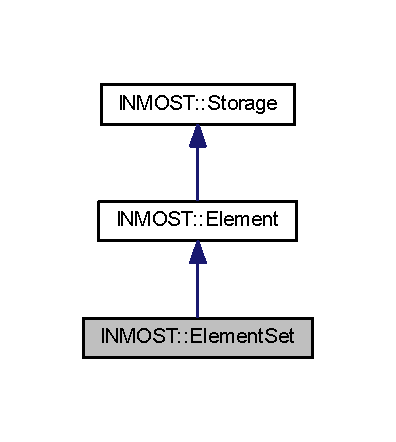
\includegraphics[width=190pt]{classINMOST_1_1ElementSet__inherit__graph}
\end{center}
\end{figure}


Collaboration diagram for I\-N\-M\-O\-S\-T\-:\-:Element\-Set\-:
\nopagebreak
\begin{figure}[H]
\begin{center}
\leavevmode
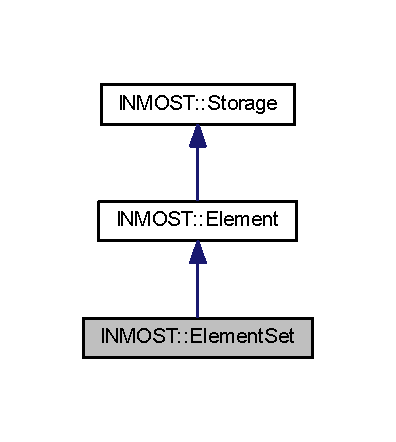
\includegraphics[width=190pt]{classINMOST_1_1ElementSet__coll__graph}
\end{center}
\end{figure}
\subsection*{Classes}
\begin{DoxyCompactItemize}
\item 
class \hyperlink{classINMOST_1_1ElementSet_1_1iterator}{iterator}
\end{DoxyCompactItemize}
\subsection*{Public Types}
\begin{DoxyCompactItemize}
\item 
\hypertarget{classINMOST_1_1ElementSet_aa2d038b0def08087dc87e30ea4ba6f36}{typedef I\-N\-M\-O\-S\-T\-\_\-\-D\-A\-T\-A\-\_\-\-B\-U\-L\-K\-\_\-\-T\-Y\-P\-E {\bfseries Comparator\-Type}}\label{classINMOST_1_1ElementSet_aa2d038b0def08087dc87e30ea4ba6f36}

\end{DoxyCompactItemize}
\subsection*{Public Member Functions}
\begin{DoxyCompactItemize}
\item 
\hypertarget{classINMOST_1_1ElementSet_a6aed94d3dcaeeaaeab9a3d9fe599d903}{{\bfseries Element\-Set} (\hyperlink{classINMOST_1_1Mesh}{Mesh} $\ast$m, Handle\-Type h)}\label{classINMOST_1_1ElementSet_a6aed94d3dcaeeaaeab9a3d9fe599d903}

\item 
\hypertarget{classINMOST_1_1ElementSet_ae58454f19b83823fbe19cf97932ba91d}{{\bfseries Element\-Set} (\hyperlink{classINMOST_1_1Mesh}{Mesh} $\ast$m, Handle\-Type $\ast$h)}\label{classINMOST_1_1ElementSet_ae58454f19b83823fbe19cf97932ba91d}

\item 
\hypertarget{classINMOST_1_1ElementSet_ae113d4ca56a6d5e9a8e6da68adb85135}{{\bfseries Element\-Set} (const \hyperlink{classINMOST_1_1Cell}{Cell} \&other)}\label{classINMOST_1_1ElementSet_ae113d4ca56a6d5e9a8e6da68adb85135}

\item 
\hypertarget{classINMOST_1_1ElementSet_a23d05143e6c17d9d0160970fe9e77f0d}{\hyperlink{classINMOST_1_1ElementSet}{Element\-Set} \& {\bfseries operator=} (\hyperlink{classINMOST_1_1ElementSet}{Element\-Set} const \&other)}\label{classINMOST_1_1ElementSet_a23d05143e6c17d9d0160970fe9e77f0d}

\item 
\hypertarget{classINMOST_1_1ElementSet_aa449d57fb308e75a4133aff074810cd8}{\hyperlink{classINMOST_1_1ElementSet}{Element\-Set} $\ast$ {\bfseries operator-\/$>$} ()}\label{classINMOST_1_1ElementSet_aa449d57fb308e75a4133aff074810cd8}

\item 
\hypertarget{classINMOST_1_1ElementSet_a30d53f550120f3233cf4a07816d70d5a}{const \hyperlink{classINMOST_1_1ElementSet}{Element\-Set} $\ast$ {\bfseries operator-\/$>$} () const }\label{classINMOST_1_1ElementSet_a30d53f550120f3233cf4a07816d70d5a}

\item 
\hypertarget{classINMOST_1_1ElementSet_a020ccd702ebc614cc4eb8b7f07ea0921}{\hyperlink{classINMOST_1_1ElementSet}{Element\-Set} \& {\bfseries self} ()}\label{classINMOST_1_1ElementSet_a020ccd702ebc614cc4eb8b7f07ea0921}

\item 
\hypertarget{classINMOST_1_1ElementSet_aac32b559e5b4134dd756f8eabb9ea6a6}{const \hyperlink{classINMOST_1_1ElementSet}{Element\-Set} \& {\bfseries self} () const }\label{classINMOST_1_1ElementSet_aac32b559e5b4134dd756f8eabb9ea6a6}

\item 
\hypertarget{classINMOST_1_1ElementSet_ad40fe14ad7209c986897a8cd4560c6fd}{std\-::string \hyperlink{classINMOST_1_1ElementSet_ad40fe14ad7209c986897a8cd4560c6fd}{Get\-Name} () const }\label{classINMOST_1_1ElementSet_ad40fe14ad7209c986897a8cd4560c6fd}

\begin{DoxyCompactList}\small\item\em Get name of the set. \end{DoxyCompactList}\item 
\hypertarget{classINMOST_1_1ElementSet_ab38d00bdde98d5b56e93f4e57927339d}{\hyperlink{classINMOST_1_1ElementSet}{Element\-Set} \hyperlink{classINMOST_1_1ElementSet_ab38d00bdde98d5b56e93f4e57927339d}{Get\-Parent} () const }\label{classINMOST_1_1ElementSet_ab38d00bdde98d5b56e93f4e57927339d}

\begin{DoxyCompactList}\small\item\em Retrieve parent of the set. \end{DoxyCompactList}\item 
\hypertarget{classINMOST_1_1ElementSet_a9231fb92dc27a9127dc4f3c8d2e22f3e}{\hyperlink{classINMOST_1_1ElementSet}{Element\-Set} \hyperlink{classINMOST_1_1ElementSet_a9231fb92dc27a9127dc4f3c8d2e22f3e}{Get\-Sibling} () const }\label{classINMOST_1_1ElementSet_a9231fb92dc27a9127dc4f3c8d2e22f3e}

\begin{DoxyCompactList}\small\item\em Retrieve sibling set of the set, this will be next child for the parent. \end{DoxyCompactList}\item 
\hyperlink{classINMOST_1_1ElementSet}{Element\-Set} \hyperlink{classINMOST_1_1ElementSet_a0b56098516de44a89002a6ec26dbd926}{Get\-Child} () const 
\begin{DoxyCompactList}\small\item\em Retrieve child set of the set. \end{DoxyCompactList}\item 
\hypertarget{classINMOST_1_1ElementSet_a5e1ad74f8bee55d751929797e514fe25}{void \hyperlink{classINMOST_1_1ElementSet_a5e1ad74f8bee55d751929797e514fe25}{Add\-Sibling} (const \hyperlink{classINMOST_1_1ElementSet}{Element\-Set} \&sibling) const }\label{classINMOST_1_1ElementSet_a5e1ad74f8bee55d751929797e514fe25}

\begin{DoxyCompactList}\small\item\em This will create new child for the parent. \end{DoxyCompactList}\item 
\hypertarget{classINMOST_1_1ElementSet_a54777ea375b83b8eb181f65fef8f9cbb}{void \hyperlink{classINMOST_1_1ElementSet_a54777ea375b83b8eb181f65fef8f9cbb}{Add\-Child} (const \hyperlink{classINMOST_1_1ElementSet}{Element\-Set} \&child) const }\label{classINMOST_1_1ElementSet_a54777ea375b83b8eb181f65fef8f9cbb}

\begin{DoxyCompactList}\small\item\em Add child to current set. \end{DoxyCompactList}\item 
\hypertarget{classINMOST_1_1ElementSet_a8993015c5cb4f251d457c0bd02f31596}{void \hyperlink{classINMOST_1_1ElementSet_a8993015c5cb4f251d457c0bd02f31596}{Rem\-Sibling} (const \hyperlink{classINMOST_1_1ElementSet}{Element\-Set} \&sibling) const }\label{classINMOST_1_1ElementSet_a8993015c5cb4f251d457c0bd02f31596}

\begin{DoxyCompactList}\small\item\em This will erase sibling or parent's child. \end{DoxyCompactList}\item 
\hypertarget{classINMOST_1_1ElementSet_aa7b86070ba51b14b5cadcf598f6edb29}{void \hyperlink{classINMOST_1_1ElementSet_aa7b86070ba51b14b5cadcf598f6edb29}{Rem\-Child} (const \hyperlink{classINMOST_1_1ElementSet}{Element\-Set} \&child) const }\label{classINMOST_1_1ElementSet_aa7b86070ba51b14b5cadcf598f6edb29}

\begin{DoxyCompactList}\small\item\em This will erase my child. \end{DoxyCompactList}\item 
\hypertarget{classINMOST_1_1ElementSet_a0e93907cddd2f9486af14f497362f761}{\hyperlink{classINMOST_1_1Storage_ae333dfced6fa9cfde0c8e7dcf1b0cc2b}{enumerator} \hyperlink{classINMOST_1_1ElementSet_a0e93907cddd2f9486af14f497362f761}{Count\-Siblings} () const }\label{classINMOST_1_1ElementSet_a0e93907cddd2f9486af14f497362f761}

\begin{DoxyCompactList}\small\item\em How many there are siblings to the right of me including me. \end{DoxyCompactList}\item 
\hypertarget{classINMOST_1_1ElementSet_abd1a5a15dde363cd7c55d77028902dd5}{\hyperlink{classINMOST_1_1Storage_ae333dfced6fa9cfde0c8e7dcf1b0cc2b}{enumerator} \hyperlink{classINMOST_1_1ElementSet_abd1a5a15dde363cd7c55d77028902dd5}{Count\-Children} () const }\label{classINMOST_1_1ElementSet_abd1a5a15dde363cd7c55d77028902dd5}

\begin{DoxyCompactList}\small\item\em How many children I have. \end{DoxyCompactList}\item 
\hypertarget{classINMOST_1_1ElementSet_a8fb6b18ca91b86090562a412d648caed}{bool {\bfseries Have\-Sibling} () const }\label{classINMOST_1_1ElementSet_a8fb6b18ca91b86090562a412d648caed}

\item 
\hypertarget{classINMOST_1_1ElementSet_a9c3a20b2d85554fa5d2abe5b59bc40b1}{bool {\bfseries Have\-Parent} () const }\label{classINMOST_1_1ElementSet_a9c3a20b2d85554fa5d2abe5b59bc40b1}

\item 
\hypertarget{classINMOST_1_1ElementSet_ae9f727556f696cf336349a4ff7ab8774}{bool {\bfseries Have\-Child} () const }\label{classINMOST_1_1ElementSet_ae9f727556f696cf336349a4ff7ab8774}

\item 
Handle\-Type $\ast$ \hyperlink{classINMOST_1_1ElementSet_a9f9a30cf2c426e7e225950c7627143f8}{get\-Handles} () const 
\begin{DoxyCompactList}\small\item\em Direct raw access to stored elements, no copy involved. \end{DoxyCompactList}\item 
\hyperlink{classINMOST_1_1Storage_ae333dfced6fa9cfde0c8e7dcf1b0cc2b}{enumerator} \hyperlink{classINMOST_1_1ElementSet_a97aa938d4e6060235056a67042b5cbe8}{nb\-Handles} () const 
\begin{DoxyCompactList}\small\item\em Retrieve number of stored handles, including invalid. \end{DoxyCompactList}\item 
\hyperlink{classINMOST_1_1Storage_ae333dfced6fa9cfde0c8e7dcf1b0cc2b}{enumerator} \hyperlink{classINMOST_1_1ElementSet_a7887bbf333dd08f1d3a8132728c1992b}{nb\-Sorted} () const 
\begin{DoxyCompactList}\small\item\em Retrieve position after last sorted element. \end{DoxyCompactList}\item 
\hypertarget{classINMOST_1_1ElementSet_a47eeee88d1c207c2cef615721013d102}{\hyperlink{classINMOST_1_1Storage_ae333dfced6fa9cfde0c8e7dcf1b0cc2b}{enumerator} \hyperlink{classINMOST_1_1ElementSet_a47eeee88d1c207c2cef615721013d102}{nb\-Adj\-Elements} (Element\-Type etype) const }\label{classINMOST_1_1ElementSet_a47eeee88d1c207c2cef615721013d102}

\begin{DoxyCompactList}\small\item\em Retrieve all elements by type. \end{DoxyCompactList}\item 
\hyperlink{classINMOST_1_1Storage_ae333dfced6fa9cfde0c8e7dcf1b0cc2b}{enumerator} \hyperlink{classINMOST_1_1ElementSet_a4d3408a6908095a029584c24701e1144}{nb\-Adj\-Elements} (Element\-Type etype, Marker\-Type select, bool invert=false) const 
\begin{DoxyCompactList}\small\item\em Retrieve number of adjacent elements with marker. \end{DoxyCompactList}\item 
\hypertarget{classINMOST_1_1ElementSet_a7ade4a7bc7ac22b929738d7bf75e3144}{\hyperlink{classINMOST_1_1ElementArray}{Element\-Array}$<$ \hyperlink{classINMOST_1_1Element}{Element} $>$ \hyperlink{classINMOST_1_1ElementSet_a7ade4a7bc7ac22b929738d7bf75e3144}{get\-Adj\-Elements} (Element\-Type etype) const }\label{classINMOST_1_1ElementSet_a7ade4a7bc7ac22b929738d7bf75e3144}

\begin{DoxyCompactList}\small\item\em Retrieve all elements by type. \end{DoxyCompactList}\item 
\hyperlink{classINMOST_1_1ElementArray}{Element\-Array}$<$ \hyperlink{classINMOST_1_1Element}{Element} $>$ \hyperlink{classINMOST_1_1ElementSet_aec40c76a04a0180105fcdddedb31da63}{get\-Adj\-Elements} (Element\-Type etype, Marker\-Type select, bool invert=false) const 
\begin{DoxyCompactList}\small\item\em Retrieve unordered array of adjacent elements with marker. \end{DoxyCompactList}\item 
\hypertarget{classINMOST_1_1ElementSet_a189d152060b36e7800c08e7d0f94fdfa}{\hyperlink{classINMOST_1_1ElementArray}{Element\-Array}$<$ \hyperlink{classINMOST_1_1Node}{Node} $>$ \hyperlink{classINMOST_1_1ElementSet_a189d152060b36e7800c08e7d0f94fdfa}{get\-Nodes} () const }\label{classINMOST_1_1ElementSet_a189d152060b36e7800c08e7d0f94fdfa}

\begin{DoxyCompactList}\small\item\em Retrieve only nodes. \end{DoxyCompactList}\item 
\hypertarget{classINMOST_1_1ElementSet_ad87ceb890eaa093e45e13475fb33ffee}{\hyperlink{classINMOST_1_1ElementArray}{Element\-Array}$<$ \hyperlink{classINMOST_1_1Node}{Node} $>$ {\bfseries get\-Nodes} (Marker\-Type select, bool invert=false) const }\label{classINMOST_1_1ElementSet_ad87ceb890eaa093e45e13475fb33ffee}

\item 
\hypertarget{classINMOST_1_1ElementSet_a89ac64c67135a46eed6475b84fe330a8}{\hyperlink{classINMOST_1_1ElementArray}{Element\-Array}$<$ \hyperlink{classINMOST_1_1Edge}{Edge} $>$ \hyperlink{classINMOST_1_1ElementSet_a89ac64c67135a46eed6475b84fe330a8}{get\-Edges} () const }\label{classINMOST_1_1ElementSet_a89ac64c67135a46eed6475b84fe330a8}

\begin{DoxyCompactList}\small\item\em Retrieve only edges. \end{DoxyCompactList}\item 
\hypertarget{classINMOST_1_1ElementSet_a723be5f10c80cec2290858117a617d75}{\hyperlink{classINMOST_1_1ElementArray}{Element\-Array}$<$ \hyperlink{classINMOST_1_1Edge}{Edge} $>$ {\bfseries get\-Edges} (Marker\-Type select, bool invert=false) const }\label{classINMOST_1_1ElementSet_a723be5f10c80cec2290858117a617d75}

\item 
\hypertarget{classINMOST_1_1ElementSet_a7b0d595c190a82196b2bbff022ef46eb}{\hyperlink{classINMOST_1_1ElementArray}{Element\-Array}$<$ \hyperlink{classINMOST_1_1Face}{Face} $>$ \hyperlink{classINMOST_1_1ElementSet_a7b0d595c190a82196b2bbff022ef46eb}{get\-Faces} () const }\label{classINMOST_1_1ElementSet_a7b0d595c190a82196b2bbff022ef46eb}

\begin{DoxyCompactList}\small\item\em Retrieve only faces. \end{DoxyCompactList}\item 
\hypertarget{classINMOST_1_1ElementSet_a37460bc42ddabbbd2b9feefc313e9a22}{\hyperlink{classINMOST_1_1ElementArray}{Element\-Array}$<$ \hyperlink{classINMOST_1_1Face}{Face} $>$ {\bfseries get\-Faces} (Marker\-Type select, bool invert=false) const }\label{classINMOST_1_1ElementSet_a37460bc42ddabbbd2b9feefc313e9a22}

\item 
\hypertarget{classINMOST_1_1ElementSet_a1ac9b271c2ddf7ea193c1f2711f59df4}{\hyperlink{classINMOST_1_1ElementArray}{Element\-Array}$<$ \hyperlink{classINMOST_1_1Cell}{Cell} $>$ \hyperlink{classINMOST_1_1ElementSet_a1ac9b271c2ddf7ea193c1f2711f59df4}{get\-Cells} () const }\label{classINMOST_1_1ElementSet_a1ac9b271c2ddf7ea193c1f2711f59df4}

\begin{DoxyCompactList}\small\item\em Retrieve only cells. \end{DoxyCompactList}\item 
\hypertarget{classINMOST_1_1ElementSet_a2e06bd0a9d9b5ffdc04560b3cdd560eb}{\hyperlink{classINMOST_1_1ElementArray}{Element\-Array}$<$ \hyperlink{classINMOST_1_1Cell}{Cell} $>$ {\bfseries get\-Cells} (Marker\-Type select, bool invert=false) const }\label{classINMOST_1_1ElementSet_a2e06bd0a9d9b5ffdc04560b3cdd560eb}

\item 
void \hyperlink{classINMOST_1_1ElementSet_a13a74a11c9b6ece25ed448bf5cb7c866}{Put\-Element} (Handle\-Type e) const 
\begin{DoxyCompactList}\small\item\em Put one element without checking of the existance of duplicate. \end{DoxyCompactList}\item 
void \hyperlink{classINMOST_1_1ElementSet_af35d9f82faa96fba32e0a4022ffe38fe}{Put\-Element} (const \hyperlink{classINMOST_1_1Storage}{Storage} \&e) const 
\begin{DoxyCompactList}\small\item\em Put one element without checking of the existance of duplicate. \end{DoxyCompactList}\item 
\hypertarget{classINMOST_1_1ElementSet_af4ef11220e0080aa1c63756af45addf9}{void \hyperlink{classINMOST_1_1ElementSet_af4ef11220e0080aa1c63756af45addf9}{Put\-Elements} (const Handle\-Type $\ast$handles, \hyperlink{classINMOST_1_1Storage_ae333dfced6fa9cfde0c8e7dcf1b0cc2b}{enumerator} num) const }\label{classINMOST_1_1ElementSet_af4ef11220e0080aa1c63756af45addf9}

\begin{DoxyCompactList}\small\item\em Put multiple handles without checking of the existance of duplicate. \end{DoxyCompactList}\item 
\hypertarget{classINMOST_1_1ElementSet_a6d09e6ad48a8746c01b0dfccb21441ae}{void \hyperlink{classINMOST_1_1ElementSet_a6d09e6ad48a8746c01b0dfccb21441ae}{Put\-Elements} (const \hyperlink{classINMOST_1_1ElementSet}{Element\-Set} \&other) const }\label{classINMOST_1_1ElementSet_a6d09e6ad48a8746c01b0dfccb21441ae}

\begin{DoxyCompactList}\small\item\em Put multiple handles of the other set without checking of the existance of duplicate. \end{DoxyCompactList}\item 
\hypertarget{classINMOST_1_1ElementSet_a2b27cedaf22cb5e20e36bcb480c9e50c}{{\footnotesize template$<$typename E\-Type $>$ }\\void \hyperlink{classINMOST_1_1ElementSet_a2b27cedaf22cb5e20e36bcb480c9e50c}{Put\-Elements} (const \hyperlink{classINMOST_1_1ElementArray}{Element\-Array}$<$ E\-Type $>$ \&elems) const }\label{classINMOST_1_1ElementSet_a2b27cedaf22cb5e20e36bcb480c9e50c}

\begin{DoxyCompactList}\small\item\em Put multiple handles without checking. \end{DoxyCompactList}\item 
void \hyperlink{classINMOST_1_1ElementSet_ad055a42db8847e0cb2465069640dd19f}{Add\-Element} (Handle\-Type e) const 
\begin{DoxyCompactList}\small\item\em Put one element with checking of the existance of duplicate. \end{DoxyCompactList}\item 
void \hyperlink{classINMOST_1_1ElementSet_a346401d86638322c22cbe6aa2b4ce5e0}{Add\-Element} (const \hyperlink{classINMOST_1_1Storage}{Storage} \&e) const 
\begin{DoxyCompactList}\small\item\em Put one element with checking of the existance of duplicate. \end{DoxyCompactList}\item 
void \hyperlink{classINMOST_1_1ElementSet_af2e19ddbc09fe43f7379ab9a30949c17}{Add\-Elements} (const Handle\-Type $\ast$handles, \hyperlink{classINMOST_1_1Storage_ae333dfced6fa9cfde0c8e7dcf1b0cc2b}{enumerator} num) const 
\begin{DoxyCompactList}\small\item\em Add multiple elements with checking of the existance of duplicate. \end{DoxyCompactList}\item 
\hypertarget{classINMOST_1_1ElementSet_addc80aa711d89d55b57885d788fba296}{void \hyperlink{classINMOST_1_1ElementSet_addc80aa711d89d55b57885d788fba296}{Add\-Elements} (const \hyperlink{classINMOST_1_1ElementSet}{Element\-Set} \&other)}\label{classINMOST_1_1ElementSet_addc80aa711d89d55b57885d788fba296}

\begin{DoxyCompactList}\small\item\em Add elements of other set. \end{DoxyCompactList}\item 
\hypertarget{classINMOST_1_1ElementSet_aba2a21178003aa2a9908ca3c090d7cb8}{{\footnotesize template$<$typename E\-Type $>$ }\\void \hyperlink{classINMOST_1_1ElementSet_aba2a21178003aa2a9908ca3c090d7cb8}{Add\-Elements} (const \hyperlink{classINMOST_1_1ElementArray}{Element\-Array}$<$ E\-Type $>$ \&elems) const }\label{classINMOST_1_1ElementSet_aba2a21178003aa2a9908ca3c090d7cb8}

\begin{DoxyCompactList}\small\item\em Add multiple elements with checking of the existance of duplicate. \end{DoxyCompactList}\item 
\hypertarget{classINMOST_1_1ElementSet_ab065f848f9feaa2aedd6214525e019f8}{void {\bfseries Remove\-Element} (const \hyperlink{classINMOST_1_1Storage}{Storage} \&e) const }\label{classINMOST_1_1ElementSet_ab065f848f9feaa2aedd6214525e019f8}

\item 
\hypertarget{classINMOST_1_1ElementSet_ac183d3760eef9515cfde84dd67847e03}{void {\bfseries Remove\-Elements} (const Handle\-Type $\ast$handles, \hyperlink{classINMOST_1_1Storage_ae333dfced6fa9cfde0c8e7dcf1b0cc2b}{enumerator} num) const }\label{classINMOST_1_1ElementSet_ac183d3760eef9515cfde84dd67847e03}

\item 
\hypertarget{classINMOST_1_1ElementSet_a119169cdf12afbca790ba53169e74af0}{{\footnotesize template$<$typename E\-Type $>$ }\\void \hyperlink{classINMOST_1_1ElementSet_a119169cdf12afbca790ba53169e74af0}{Remove\-Elements} (const \hyperlink{classINMOST_1_1ElementArray}{Element\-Array}$<$ E\-Type $>$ \&elems) const }\label{classINMOST_1_1ElementSet_a119169cdf12afbca790ba53169e74af0}

\begin{DoxyCompactList}\small\item\em Remove multiple elements from the set. \end{DoxyCompactList}\item 
\hyperlink{classINMOST_1_1ElementArray}{Element\-Array}$<$ \hyperlink{classINMOST_1_1Element}{Element} $>$ \hyperlink{classINMOST_1_1ElementSet_a9d91f6c5139e8c0a0f31bf8543729bf4}{Union} (const \hyperlink{classINMOST_1_1ElementSet}{Element\-Set} \&other) const 
\begin{DoxyCompactList}\small\item\em Compute and return union with other set. \end{DoxyCompactList}\item 
\hyperlink{classINMOST_1_1ElementArray}{Element\-Array}$<$ \hyperlink{classINMOST_1_1Element}{Element} $>$ \hyperlink{classINMOST_1_1ElementSet_aba75cf7b89c6ae0b5ac41ad7f46c9df8}{Union} (const Handle\-Type $\ast$handles, \hyperlink{classINMOST_1_1Storage_ae333dfced6fa9cfde0c8e7dcf1b0cc2b}{enumerator} num) const 
\begin{DoxyCompactList}\small\item\em Compute and return union with raw handles. \end{DoxyCompactList}\item 
\hypertarget{classINMOST_1_1ElementSet_ab1ef60891bc6e6e8c095065843b51217}{{\footnotesize template$<$typename E\-Type $>$ }\\\hyperlink{classINMOST_1_1ElementArray}{Element\-Array}$<$ \hyperlink{classINMOST_1_1Element}{Element} $>$ \hyperlink{classINMOST_1_1ElementSet_ab1ef60891bc6e6e8c095065843b51217}{Union} (const \hyperlink{classINMOST_1_1ElementArray}{Element\-Array}$<$ E\-Type $>$ \&elems) const }\label{classINMOST_1_1ElementSet_ab1ef60891bc6e6e8c095065843b51217}

\begin{DoxyCompactList}\small\item\em Compute and return union with elements. \end{DoxyCompactList}\item 
\hypertarget{classINMOST_1_1ElementSet_a8e28cfda634eec4ffcf892209bf9899a}{\hyperlink{classINMOST_1_1ElementArray}{Element\-Array}$<$ \hyperlink{classINMOST_1_1Element}{Element} $>$ {\bfseries Difference} (const \hyperlink{classINMOST_1_1ElementSet}{Element\-Set} \&other) const }\label{classINMOST_1_1ElementSet_a8e28cfda634eec4ffcf892209bf9899a}

\item 
\hyperlink{classINMOST_1_1ElementArray}{Element\-Array}$<$ \hyperlink{classINMOST_1_1Element}{Element} $>$ \hyperlink{classINMOST_1_1ElementSet_a4b7496ef3146d869c4b8db7ba378d152}{Difference} (const Handle\-Type $\ast$handles, \hyperlink{classINMOST_1_1Storage_ae333dfced6fa9cfde0c8e7dcf1b0cc2b}{enumerator} num) const 
\begin{DoxyCompactList}\small\item\em Compute and return difference with raw handles. \end{DoxyCompactList}\item 
\hypertarget{classINMOST_1_1ElementSet_af038e8851f02e9c4ae488a3ed1530bd7}{{\footnotesize template$<$typename E\-Type $>$ }\\\hyperlink{classINMOST_1_1ElementArray}{Element\-Array}$<$ \hyperlink{classINMOST_1_1Element}{Element} $>$ \hyperlink{classINMOST_1_1ElementSet_af038e8851f02e9c4ae488a3ed1530bd7}{Difference} (const \hyperlink{classINMOST_1_1ElementArray}{Element\-Array}$<$ E\-Type $>$ \&elems) const }\label{classINMOST_1_1ElementSet_af038e8851f02e9c4ae488a3ed1530bd7}

\begin{DoxyCompactList}\small\item\em Compute and return difference with elements. \end{DoxyCompactList}\item 
\hypertarget{classINMOST_1_1ElementSet_a9db0add67c5ca85db968f77bf7162e2c}{\hyperlink{classINMOST_1_1ElementArray}{Element\-Array}$<$ \hyperlink{classINMOST_1_1Element}{Element} $>$ {\bfseries Intersection} (const \hyperlink{classINMOST_1_1ElementSet}{Element\-Set} \&other) const }\label{classINMOST_1_1ElementSet_a9db0add67c5ca85db968f77bf7162e2c}

\item 
\hyperlink{classINMOST_1_1ElementArray}{Element\-Array}$<$ \hyperlink{classINMOST_1_1Element}{Element} $>$ \hyperlink{classINMOST_1_1ElementSet_a2afffba16c7c38cf23a6a0706af45d27}{Intersection} (const Handle\-Type $\ast$handles, \hyperlink{classINMOST_1_1Storage_ae333dfced6fa9cfde0c8e7dcf1b0cc2b}{enumerator} num) const 
\begin{DoxyCompactList}\small\item\em Compute and return intersection with raw handles. \end{DoxyCompactList}\item 
\hypertarget{classINMOST_1_1ElementSet_a9991abefdf4ecfdf35ee2d52eea650f1}{{\footnotesize template$<$typename E\-Type $>$ }\\\hyperlink{classINMOST_1_1ElementArray}{Element\-Array}$<$ \hyperlink{classINMOST_1_1Element}{Element} $>$ \hyperlink{classINMOST_1_1ElementSet_a9991abefdf4ecfdf35ee2d52eea650f1}{Intersection} (const \hyperlink{classINMOST_1_1ElementArray}{Element\-Array}$<$ E\-Type $>$ \&elems) const }\label{classINMOST_1_1ElementSet_a9991abefdf4ecfdf35ee2d52eea650f1}

\begin{DoxyCompactList}\small\item\em Compute and return intersection with elements. \end{DoxyCompactList}\item 
\hypertarget{classINMOST_1_1ElementSet_a844bc0a82eb19514e7033bc831df0a9e}{void \hyperlink{classINMOST_1_1ElementSet_a844bc0a82eb19514e7033bc831df0a9e}{Unite} (const \hyperlink{classINMOST_1_1ElementSet}{Element\-Set} \&other) const }\label{classINMOST_1_1ElementSet_a844bc0a82eb19514e7033bc831df0a9e}

\begin{DoxyCompactList}\small\item\em Compute and store union with raw handles. \end{DoxyCompactList}\item 
\hypertarget{classINMOST_1_1ElementSet_ae591fb8fad3f163e8c26c264db8f6e4c}{void \hyperlink{classINMOST_1_1ElementSet_ae591fb8fad3f163e8c26c264db8f6e4c}{Unite} (const Handle\-Type $\ast$handles, \hyperlink{classINMOST_1_1Storage_ae333dfced6fa9cfde0c8e7dcf1b0cc2b}{enumerator} num) const }\label{classINMOST_1_1ElementSet_ae591fb8fad3f163e8c26c264db8f6e4c}

\begin{DoxyCompactList}\small\item\em Compute and store union with raw handles. \end{DoxyCompactList}\item 
\hypertarget{classINMOST_1_1ElementSet_af22386930e063d805c1961222e202b24}{{\footnotesize template$<$typename E\-Type $>$ }\\void \hyperlink{classINMOST_1_1ElementSet_af22386930e063d805c1961222e202b24}{Unite} (const \hyperlink{classINMOST_1_1ElementArray}{Element\-Array}$<$ E\-Type $>$ \&elems) const }\label{classINMOST_1_1ElementSet_af22386930e063d805c1961222e202b24}

\begin{DoxyCompactList}\small\item\em Compute and store union with elements. \end{DoxyCompactList}\item 
void \hyperlink{classINMOST_1_1ElementSet_a1aafea0ac742bcc3ec1873621ca41ccd}{Subtract} (const \hyperlink{classINMOST_1_1ElementSet}{Element\-Set} \&other) const 
\begin{DoxyCompactList}\small\item\em Compute and store difference with raw handles. \end{DoxyCompactList}\item 
\hypertarget{classINMOST_1_1ElementSet_aa61d299bbf8d4fd4c67a983c2139fbe5}{void \hyperlink{classINMOST_1_1ElementSet_aa61d299bbf8d4fd4c67a983c2139fbe5}{Subtract} (const Handle\-Type $\ast$handles, \hyperlink{classINMOST_1_1Storage_ae333dfced6fa9cfde0c8e7dcf1b0cc2b}{enumerator} num) const }\label{classINMOST_1_1ElementSet_aa61d299bbf8d4fd4c67a983c2139fbe5}

\begin{DoxyCompactList}\small\item\em Compute and store difference with raw handles. \end{DoxyCompactList}\item 
\hypertarget{classINMOST_1_1ElementSet_aa4a51ad66c30dbc1d55618a25901599e}{{\footnotesize template$<$typename E\-Type $>$ }\\void \hyperlink{classINMOST_1_1ElementSet_aa4a51ad66c30dbc1d55618a25901599e}{Subtract} (const \hyperlink{classINMOST_1_1ElementArray}{Element\-Array}$<$ E\-Type $>$ \&elems) const }\label{classINMOST_1_1ElementSet_aa4a51ad66c30dbc1d55618a25901599e}

\begin{DoxyCompactList}\small\item\em Compute and store difference with elements. \end{DoxyCompactList}\item 
\hypertarget{classINMOST_1_1ElementSet_a038b4d38d59f5d955fe54edffec42b02}{void \hyperlink{classINMOST_1_1ElementSet_a038b4d38d59f5d955fe54edffec42b02}{Intersect} (const \hyperlink{classINMOST_1_1ElementSet}{Element\-Set} \&other) const }\label{classINMOST_1_1ElementSet_a038b4d38d59f5d955fe54edffec42b02}

\begin{DoxyCompactList}\small\item\em Compute and store intersection with raw handles. \end{DoxyCompactList}\item 
\hypertarget{classINMOST_1_1ElementSet_ad16933df1e7aca014a50062e93f571b9}{void \hyperlink{classINMOST_1_1ElementSet_ad16933df1e7aca014a50062e93f571b9}{Intersect} (const Handle\-Type $\ast$handles, \hyperlink{classINMOST_1_1Storage_ae333dfced6fa9cfde0c8e7dcf1b0cc2b}{enumerator} num) const }\label{classINMOST_1_1ElementSet_ad16933df1e7aca014a50062e93f571b9}

\begin{DoxyCompactList}\small\item\em Compute and store intersection with raw handles. \end{DoxyCompactList}\item 
\hypertarget{classINMOST_1_1ElementSet_a361a4f92a43b559c554554cf7492670a}{{\footnotesize template$<$typename E\-Type $>$ }\\void \hyperlink{classINMOST_1_1ElementSet_a361a4f92a43b559c554554cf7492670a}{Intersect} (const \hyperlink{classINMOST_1_1ElementArray}{Element\-Array}$<$ E\-Type $>$ \&elems) const }\label{classINMOST_1_1ElementSet_a361a4f92a43b559c554554cf7492670a}

\begin{DoxyCompactList}\small\item\em Compute and store intersection with elements. \end{DoxyCompactList}\item 
void \hyperlink{classINMOST_1_1ElementSet_a96676712005ce12f0c1f9a92c6ac095d}{Sort\-Set} (Comparator\-Type comp) const 
\begin{DoxyCompactList}\small\item\em Performs sort of the set of elements. \end{DoxyCompactList}\item 
\hyperlink{classINMOST_1_1Element}{Element} \hyperlink{classINMOST_1_1ElementSet_aa4fac35a59d299c9dca99b0434a127e7}{Find\-Element\-By\-Global\-I\-D} (\hyperlink{classINMOST_1_1Storage_aec96942bc647417a801e2895b45964d2}{integer} global\-\_\-id) const 
\begin{DoxyCompactList}\small\item\em Perform binary search by global id. \end{DoxyCompactList}\item 
\hyperlink{classINMOST_1_1Element}{Element} \hyperlink{classINMOST_1_1ElementSet_ad1921b1662920da28e5f958fd397f448}{Find\-Element\-By\-Centroid} (\hyperlink{classINMOST_1_1Storage_a853346784b4a5822a7fac54d8f10f805}{real} $\ast$centroid) const 
\begin{DoxyCompactList}\small\item\em Perform binary search by centroid. \end{DoxyCompactList}\item 
bool \hyperlink{classINMOST_1_1ElementSet_acb23b3c8a46fe1b04d486cf4a173365a}{Find\-Handle} (Handle\-Type h, bool use\-\_\-comparator) const 
\begin{DoxyCompactList}\small\item\em Performs linear search in unsorted set. \end{DoxyCompactList}\item 
\hypertarget{classINMOST_1_1ElementSet_a17022215a9a701dfad2e77b3eb8c1429}{void \hyperlink{classINMOST_1_1ElementSet_a17022215a9a701dfad2e77b3eb8c1429}{Set\-Marker\-Elements} (Marker\-Type m, Element\-Type etype=E\-S\-E\-T$|$C\-E\-L\-L$|$F\-A\-C\-E$|$E\-D\-G\-E$|$N\-O\-D\-E) const }\label{classINMOST_1_1ElementSet_a17022215a9a701dfad2e77b3eb8c1429}

\begin{DoxyCompactList}\small\item\em Set markers on all the elements of given type. \end{DoxyCompactList}\item 
\hypertarget{classINMOST_1_1ElementSet_afa202ba264c8c6993c3943586f6dd4ee}{void \hyperlink{classINMOST_1_1ElementSet_afa202ba264c8c6993c3943586f6dd4ee}{Rem\-Marker\-Elements} (Marker\-Type m, Element\-Type etype=E\-S\-E\-T$|$C\-E\-L\-L$|$F\-A\-C\-E$|$E\-D\-G\-E$|$N\-O\-D\-E) const }\label{classINMOST_1_1ElementSet_afa202ba264c8c6993c3943586f6dd4ee}

\begin{DoxyCompactList}\small\item\em Remove markers from all the elements of given type. \end{DoxyCompactList}\item 
\hyperlink{classINMOST_1_1ElementSet_1_1iterator}{iterator} \hyperlink{classINMOST_1_1ElementSet_ad43c994c6cc58c382aa12e0705048226}{Begin} () const 
\begin{DoxyCompactList}\small\item\em Provides forward iterator that skips deleted and hidden elements within set. \end{DoxyCompactList}\item 
\hyperlink{classINMOST_1_1ElementSet_1_1iterator}{iterator} \hyperlink{classINMOST_1_1ElementSet_a5174eb80bbdbc6c68bee4b0f33eef46a}{End} () const 
\begin{DoxyCompactList}\small\item\em Provides end for forward iterator to stop the loop. \end{DoxyCompactList}\item 
\hyperlink{classINMOST_1_1ElementSet_1_1iterator}{iterator} \hyperlink{classINMOST_1_1ElementSet_a1d6d3edcf969e5a1c072224433783ea2}{End\-Sorted} () const 
\begin{DoxyCompactList}\small\item\em Provides iterator that points to element located after the last element that belong to presorted part of the set as well as on the first element of unsorted part. \end{DoxyCompactList}\item 
\hypertarget{classINMOST_1_1ElementSet_a70c7f2c20ecbc61eb65ef6013b2cf6e2}{\hyperlink{classINMOST_1_1ElementSet_1_1iterator}{iterator} \hyperlink{classINMOST_1_1ElementSet_a70c7f2c20ecbc61eb65ef6013b2cf6e2}{Erase} (\hyperlink{classINMOST_1_1ElementSet_1_1iterator}{iterator} pos) const }\label{classINMOST_1_1ElementSet_a70c7f2c20ecbc61eb65ef6013b2cf6e2}

\begin{DoxyCompactList}\small\item\em Erase one element pointed by iterator and return next valid element. \end{DoxyCompactList}\item 
\hypertarget{classINMOST_1_1ElementSet_a9a7725f9cf622fa8ff01b26a88aedb1e}{void \hyperlink{classINMOST_1_1ElementSet_a9a7725f9cf622fa8ff01b26a88aedb1e}{Erase} (\hyperlink{classINMOST_1_1ElementSet_1_1iterator}{iterator} beg, \hyperlink{classINMOST_1_1ElementSet_1_1iterator}{iterator} end) const }\label{classINMOST_1_1ElementSet_a9a7725f9cf622fa8ff01b26a88aedb1e}

\begin{DoxyCompactList}\small\item\em Erase set of elements pointed by iterators. \end{DoxyCompactList}\item 
\hypertarget{classINMOST_1_1ElementSet_a9a01902cdfb305404da949ec26bada4f}{Comparator\-Type \hyperlink{classINMOST_1_1ElementSet_a9a01902cdfb305404da949ec26bada4f}{Get\-Comparator} () const }\label{classINMOST_1_1ElementSet_a9a01902cdfb305404da949ec26bada4f}

\begin{DoxyCompactList}\small\item\em Retrieve current set comparator. \end{DoxyCompactList}\item 
\hypertarget{classINMOST_1_1ElementSet_a4315de813986b2824dbc7aedb15c6624}{void \hyperlink{classINMOST_1_1ElementSet_a4315de813986b2824dbc7aedb15c6624}{Reorder\-Empty} () const }\label{classINMOST_1_1ElementSet_a4315de813986b2824dbc7aedb15c6624}

\begin{DoxyCompactList}\small\item\em Compact holes in inner representation. \end{DoxyCompactList}\item 
\hypertarget{classINMOST_1_1ElementSet_a2bcfc456bd891780f082f054ccb2c301}{bool \hyperlink{classINMOST_1_1ElementSet_a2bcfc456bd891780f082f054ccb2c301}{Empty} () const }\label{classINMOST_1_1ElementSet_a2bcfc456bd891780f082f054ccb2c301}

\begin{DoxyCompactList}\small\item\em Is there any elements in the set. \end{DoxyCompactList}\item 
\hypertarget{classINMOST_1_1ElementSet_a58214190b41f9ed069ff37c0a49281c9}{\hyperlink{classINMOST_1_1Storage_ae333dfced6fa9cfde0c8e7dcf1b0cc2b}{enumerator} \hyperlink{classINMOST_1_1ElementSet_a58214190b41f9ed069ff37c0a49281c9}{Size} () const }\label{classINMOST_1_1ElementSet_a58214190b41f9ed069ff37c0a49281c9}

\begin{DoxyCompactList}\small\item\em Get total number of elements. \end{DoxyCompactList}\item 
\hypertarget{classINMOST_1_1ElementSet_a70f53036c6119d8c163cd27e1e5758d7}{void \hyperlink{classINMOST_1_1ElementSet_a70f53036c6119d8c163cd27e1e5758d7}{Clear} () const }\label{classINMOST_1_1ElementSet_a70f53036c6119d8c163cd27e1e5758d7}

\begin{DoxyCompactList}\small\item\em Remove all elements, clear all data, removes sorted marker. \end{DoxyCompactList}\end{DoxyCompactItemize}
\subsection*{Static Public Attributes}
\begin{DoxyCompactItemize}
\item 
static const \hyperlink{classINMOST_1_1Storage_ae333dfced6fa9cfde0c8e7dcf1b0cc2b}{enumerator} \hyperlink{classINMOST_1_1ElementSet_a2a6e9c51357ae2e322d1d63118df85b8}{high\-\_\-conn\-\_\-reserved} = 4
\begin{DoxyCompactList}\small\item\em number of reserved positions in High\-Conn array. \end{DoxyCompactList}\item 
\hypertarget{classINMOST_1_1ElementSet_a094cd1d3991fb611b9bfdcfc1373b589}{static const Comparator\-Type {\bfseries U\-N\-S\-O\-R\-T\-E\-D\-\_\-\-C\-O\-M\-P\-A\-R\-A\-T\-O\-R} = 0}\label{classINMOST_1_1ElementSet_a094cd1d3991fb611b9bfdcfc1373b589}

\item 
\hypertarget{classINMOST_1_1ElementSet_af8f036b8b6e777284877e95b6ffc9df5}{static const Comparator\-Type {\bfseries G\-L\-O\-B\-A\-L\-I\-D\-\_\-\-C\-O\-M\-P\-A\-R\-A\-T\-O\-R} = 1}\label{classINMOST_1_1ElementSet_af8f036b8b6e777284877e95b6ffc9df5}

\item 
\hypertarget{classINMOST_1_1ElementSet_a0bd06415bfef0096fed9a0e4ad4b4e50}{static const Comparator\-Type {\bfseries C\-E\-N\-T\-R\-O\-I\-D\-\_\-\-C\-O\-M\-P\-A\-R\-A\-T\-O\-R} = 2}\label{classINMOST_1_1ElementSet_a0bd06415bfef0096fed9a0e4ad4b4e50}

\item 
\hypertarget{classINMOST_1_1ElementSet_a7b52a3764ca783af88e51b9942e0106f}{static const Comparator\-Type {\bfseries I\-E\-R\-A\-R\-H\-Y\-\_\-\-C\-O\-M\-P\-A\-R\-A\-T\-O\-R} = 3}\label{classINMOST_1_1ElementSet_a7b52a3764ca783af88e51b9942e0106f}

\item 
\hypertarget{classINMOST_1_1ElementSet_ac2764455c0e4bb5e1220e01995221a79}{static const Comparator\-Type {\bfseries H\-A\-N\-D\-L\-E\-\_\-\-C\-O\-M\-P\-A\-R\-A\-T\-O\-R} = 4}\label{classINMOST_1_1ElementSet_ac2764455c0e4bb5e1220e01995221a79}

\end{DoxyCompactItemize}
\subsection*{Additional Inherited Members}


\subsection{Member Function Documentation}
\hypertarget{classINMOST_1_1ElementSet_ad055a42db8847e0cb2465069640dd19f}{\index{I\-N\-M\-O\-S\-T\-::\-Element\-Set@{I\-N\-M\-O\-S\-T\-::\-Element\-Set}!Add\-Element@{Add\-Element}}
\index{Add\-Element@{Add\-Element}!INMOST::ElementSet@{I\-N\-M\-O\-S\-T\-::\-Element\-Set}}
\subsubsection[{Add\-Element}]{\setlength{\rightskip}{0pt plus 5cm}void I\-N\-M\-O\-S\-T\-::\-Element\-Set\-::\-Add\-Element (
\begin{DoxyParamCaption}
\item[{Handle\-Type}]{e}
\end{DoxyParamCaption}
) const}}\label{classINMOST_1_1ElementSet_ad055a42db8847e0cb2465069640dd19f}


Put one element with checking of the existance of duplicate. 

Preserves order for sorted set, thus may be expensive \hypertarget{classINMOST_1_1ElementSet_a346401d86638322c22cbe6aa2b4ce5e0}{\index{I\-N\-M\-O\-S\-T\-::\-Element\-Set@{I\-N\-M\-O\-S\-T\-::\-Element\-Set}!Add\-Element@{Add\-Element}}
\index{Add\-Element@{Add\-Element}!INMOST::ElementSet@{I\-N\-M\-O\-S\-T\-::\-Element\-Set}}
\subsubsection[{Add\-Element}]{\setlength{\rightskip}{0pt plus 5cm}void I\-N\-M\-O\-S\-T\-::\-Element\-Set\-::\-Add\-Element (
\begin{DoxyParamCaption}
\item[{const {\bf Storage} \&}]{e}
\end{DoxyParamCaption}
) const\hspace{0.3cm}{\ttfamily [inline]}}}\label{classINMOST_1_1ElementSet_a346401d86638322c22cbe6aa2b4ce5e0}


Put one element with checking of the existance of duplicate. 

Preserves order for sorted set, thus may be expensive \hypertarget{classINMOST_1_1ElementSet_af2e19ddbc09fe43f7379ab9a30949c17}{\index{I\-N\-M\-O\-S\-T\-::\-Element\-Set@{I\-N\-M\-O\-S\-T\-::\-Element\-Set}!Add\-Elements@{Add\-Elements}}
\index{Add\-Elements@{Add\-Elements}!INMOST::ElementSet@{I\-N\-M\-O\-S\-T\-::\-Element\-Set}}
\subsubsection[{Add\-Elements}]{\setlength{\rightskip}{0pt plus 5cm}void I\-N\-M\-O\-S\-T\-::\-Element\-Set\-::\-Add\-Elements (
\begin{DoxyParamCaption}
\item[{const Handle\-Type $\ast$}]{handles, }
\item[{{\bf enumerator}}]{num}
\end{DoxyParamCaption}
) const}}\label{classINMOST_1_1ElementSet_af2e19ddbc09fe43f7379ab9a30949c17}


Add multiple elements with checking of the existance of duplicate. 

Preserves order for sorted set, thus may be expensive. This will also remove any duplicates in unsorted part of the set. If you inserted duplicated elements through Put\-Elements into previously sorted array then this operation does not guarantee that those duplications will be stored. \hypertarget{classINMOST_1_1ElementSet_ad43c994c6cc58c382aa12e0705048226}{\index{I\-N\-M\-O\-S\-T\-::\-Element\-Set@{I\-N\-M\-O\-S\-T\-::\-Element\-Set}!Begin@{Begin}}
\index{Begin@{Begin}!INMOST::ElementSet@{I\-N\-M\-O\-S\-T\-::\-Element\-Set}}
\subsubsection[{Begin}]{\setlength{\rightskip}{0pt plus 5cm}{\bf iterator} I\-N\-M\-O\-S\-T\-::\-Element\-Set\-::\-Begin (
\begin{DoxyParamCaption}
{}
\end{DoxyParamCaption}
) const}}\label{classINMOST_1_1ElementSet_ad43c994c6cc58c382aa12e0705048226}


Provides forward iterator that skips deleted and hidden elements within set. 

The iterator will be valid during removal or insertion of elements. While that may seem usefull, many functions like Add\-Elements, Sort\-Set, Union will internally reorder handles thus making iterators useless. To correctly resolve situation when size of array shrink due to removal of elements use less then ($<$) instead of not equal (!=) operator to check for end of the loop. Note that iterators would not let you change underlaying handles, you can use get\-Handles for that instead. \begin{DoxyReturn}{Returns}
iterator that points to the first valid element 
\end{DoxyReturn}
\hypertarget{classINMOST_1_1ElementSet_a4b7496ef3146d869c4b8db7ba378d152}{\index{I\-N\-M\-O\-S\-T\-::\-Element\-Set@{I\-N\-M\-O\-S\-T\-::\-Element\-Set}!Difference@{Difference}}
\index{Difference@{Difference}!INMOST::ElementSet@{I\-N\-M\-O\-S\-T\-::\-Element\-Set}}
\subsubsection[{Difference}]{\setlength{\rightskip}{0pt plus 5cm}{\bf Element\-Array}$<${\bf Element}$>$ I\-N\-M\-O\-S\-T\-::\-Element\-Set\-::\-Difference (
\begin{DoxyParamCaption}
\item[{const Handle\-Type $\ast$}]{handles, }
\item[{{\bf enumerator}}]{num}
\end{DoxyParamCaption}
) const}}\label{classINMOST_1_1ElementSet_a4b7496ef3146d869c4b8db7ba378d152}


Compute and return difference with raw handles. 

If initial set was ordered, result will preserve the order. All elements will be unique. \hypertarget{classINMOST_1_1ElementSet_a5174eb80bbdbc6c68bee4b0f33eef46a}{\index{I\-N\-M\-O\-S\-T\-::\-Element\-Set@{I\-N\-M\-O\-S\-T\-::\-Element\-Set}!End@{End}}
\index{End@{End}!INMOST::ElementSet@{I\-N\-M\-O\-S\-T\-::\-Element\-Set}}
\subsubsection[{End}]{\setlength{\rightskip}{0pt plus 5cm}{\bf iterator} I\-N\-M\-O\-S\-T\-::\-Element\-Set\-::\-End (
\begin{DoxyParamCaption}
{}
\end{DoxyParamCaption}
) const}}\label{classINMOST_1_1ElementSet_a5174eb80bbdbc6c68bee4b0f33eef46a}


Provides end for forward iterator to stop the loop. 

\begin{DoxyReturn}{Returns}
iterator that points to the position after last element 
\end{DoxyReturn}
\hypertarget{classINMOST_1_1ElementSet_a1d6d3edcf969e5a1c072224433783ea2}{\index{I\-N\-M\-O\-S\-T\-::\-Element\-Set@{I\-N\-M\-O\-S\-T\-::\-Element\-Set}!End\-Sorted@{End\-Sorted}}
\index{End\-Sorted@{End\-Sorted}!INMOST::ElementSet@{I\-N\-M\-O\-S\-T\-::\-Element\-Set}}
\subsubsection[{End\-Sorted}]{\setlength{\rightskip}{0pt plus 5cm}{\bf iterator} I\-N\-M\-O\-S\-T\-::\-Element\-Set\-::\-End\-Sorted (
\begin{DoxyParamCaption}
{}
\end{DoxyParamCaption}
) const}}\label{classINMOST_1_1ElementSet_a1d6d3edcf969e5a1c072224433783ea2}


Provides iterator that points to element located after the last element that belong to presorted part of the set as well as on the first element of unsorted part. 

\begin{DoxyReturn}{Returns}
see description 
\end{DoxyReturn}
\hypertarget{classINMOST_1_1ElementSet_ad1921b1662920da28e5f958fd397f448}{\index{I\-N\-M\-O\-S\-T\-::\-Element\-Set@{I\-N\-M\-O\-S\-T\-::\-Element\-Set}!Find\-Element\-By\-Centroid@{Find\-Element\-By\-Centroid}}
\index{Find\-Element\-By\-Centroid@{Find\-Element\-By\-Centroid}!INMOST::ElementSet@{I\-N\-M\-O\-S\-T\-::\-Element\-Set}}
\subsubsection[{Find\-Element\-By\-Centroid}]{\setlength{\rightskip}{0pt plus 5cm}{\bf Element} I\-N\-M\-O\-S\-T\-::\-Element\-Set\-::\-Find\-Element\-By\-Centroid (
\begin{DoxyParamCaption}
\item[{{\bf real} $\ast$}]{centroid}
\end{DoxyParamCaption}
) const}}\label{classINMOST_1_1ElementSet_ad1921b1662920da28e5f958fd397f448}


Perform binary search by centroid. 

In set sorted with C\-E\-N\-T\-R\-O\-I\-D\-\_\-\-C\-O\-M\-P\-A\-R\-A\-T\-O\-R in O(log(n)) time otherwise search needs O(n) comparisons \hypertarget{classINMOST_1_1ElementSet_aa4fac35a59d299c9dca99b0434a127e7}{\index{I\-N\-M\-O\-S\-T\-::\-Element\-Set@{I\-N\-M\-O\-S\-T\-::\-Element\-Set}!Find\-Element\-By\-Global\-I\-D@{Find\-Element\-By\-Global\-I\-D}}
\index{Find\-Element\-By\-Global\-I\-D@{Find\-Element\-By\-Global\-I\-D}!INMOST::ElementSet@{I\-N\-M\-O\-S\-T\-::\-Element\-Set}}
\subsubsection[{Find\-Element\-By\-Global\-I\-D}]{\setlength{\rightskip}{0pt plus 5cm}{\bf Element} I\-N\-M\-O\-S\-T\-::\-Element\-Set\-::\-Find\-Element\-By\-Global\-I\-D (
\begin{DoxyParamCaption}
\item[{{\bf integer}}]{global\-\_\-id}
\end{DoxyParamCaption}
) const}}\label{classINMOST_1_1ElementSet_aa4fac35a59d299c9dca99b0434a127e7}


Perform binary search by global id. 

In set sorted with G\-L\-O\-B\-A\-L\-I\-D\-\_\-\-C\-O\-M\-P\-A\-R\-A\-T\-O\-R in O(log(n)) time otherwise search needs O(n) comparisons \hypertarget{classINMOST_1_1ElementSet_acb23b3c8a46fe1b04d486cf4a173365a}{\index{I\-N\-M\-O\-S\-T\-::\-Element\-Set@{I\-N\-M\-O\-S\-T\-::\-Element\-Set}!Find\-Handle@{Find\-Handle}}
\index{Find\-Handle@{Find\-Handle}!INMOST::ElementSet@{I\-N\-M\-O\-S\-T\-::\-Element\-Set}}
\subsubsection[{Find\-Handle}]{\setlength{\rightskip}{0pt plus 5cm}bool I\-N\-M\-O\-S\-T\-::\-Element\-Set\-::\-Find\-Handle (
\begin{DoxyParamCaption}
\item[{Handle\-Type}]{h, }
\item[{bool}]{use\-\_\-comparator}
\end{DoxyParamCaption}
) const}}\label{classINMOST_1_1ElementSet_acb23b3c8a46fe1b04d486cf4a173365a}


Performs linear search in unsorted set. 


\begin{DoxyItemize}
\item binary search by handle in set sorted with H\-A\-N\-D\-L\-E\-\_\-\-C\-O\-M\-P\-A\-R\-A\-T\-O\-R
\item binary search by centroid in set sorted with C\-E\-N\-T\-R\-O\-I\-D\-\_\-\-C\-O\-M\-P\-A\-R\-A\-T\-O\-R
\item binary search by global id in set sorted with G\-L\-O\-B\-A\-L\-I\-D\-\_\-\-C\-O\-M\-P\-A\-R\-A\-T\-O\-R
\item binary search by ierarhy in set sorted with I\-E\-R\-A\-R\-H\-Y\-\_\-\-C\-O\-M\-P\-A\-R\-A\-T\-O\-R (may be too expensive)
\end{DoxyItemize}

If you have a lot of elements to test against set, then you'd better first put marker on elements of the set by Set\-Marker\-Elements then test which of your elements have marker and then remove markers by Rem\-Marker\-Elements. This will consume only O(n+m) operations where n is the number of my elements and m is the size of the test set. 
\begin{DoxyParams}{Parameters}
{\em h} & handle of element \\
\hline
{\em use\-\_\-comparator} & use information about current comparator or perform linear search \\
\hline
\end{DoxyParams}
\begin{DoxyReturn}{Returns}
true if element is present 
\end{DoxyReturn}
\begin{DoxySeeAlso}{See Also}
\hyperlink{classINMOST_1_1ElementSet_a17022215a9a701dfad2e77b3eb8c1429}{Element\-Set\-::\-Set\-Marker\-Elements} 

\hyperlink{classINMOST_1_1ElementSet_afa202ba264c8c6993c3943586f6dd4ee}{Element\-Set\-::\-Rem\-Marker\-Elements} 
\end{DoxySeeAlso}
\hypertarget{classINMOST_1_1ElementSet_aec40c76a04a0180105fcdddedb31da63}{\index{I\-N\-M\-O\-S\-T\-::\-Element\-Set@{I\-N\-M\-O\-S\-T\-::\-Element\-Set}!get\-Adj\-Elements@{get\-Adj\-Elements}}
\index{get\-Adj\-Elements@{get\-Adj\-Elements}!INMOST::ElementSet@{I\-N\-M\-O\-S\-T\-::\-Element\-Set}}
\subsubsection[{get\-Adj\-Elements}]{\setlength{\rightskip}{0pt plus 5cm}{\bf Element\-Array}$<${\bf Element}$>$ I\-N\-M\-O\-S\-T\-::\-Element\-Set\-::get\-Adj\-Elements (
\begin{DoxyParamCaption}
\item[{Element\-Type}]{etype, }
\item[{Marker\-Type}]{mask, }
\item[{bool}]{invert\-\_\-mask = {\ttfamily false}}
\end{DoxyParamCaption}
) const\hspace{0.3cm}{\ttfamily [virtual]}}}\label{classINMOST_1_1ElementSet_aec40c76a04a0180105fcdddedb31da63}


Retrieve unordered array of adjacent elements with marker. 


\begin{DoxyParams}{Parameters}
{\em etype} & bitwise mask of element types \\
\hline
{\em mask} & marker to be set \\
\hline
{\em invert\-\_\-mask} & if true then those are selected on wich marker is not set \\
\hline
\end{DoxyParams}
\begin{DoxyReturn}{Returns}
array of elements 
\end{DoxyReturn}


Reimplemented from \hyperlink{classINMOST_1_1Element_ae1b2cbfce7af2e3f38f5a19d2a9a30a1}{I\-N\-M\-O\-S\-T\-::\-Element}.

\hypertarget{classINMOST_1_1ElementSet_a0b56098516de44a89002a6ec26dbd926}{\index{I\-N\-M\-O\-S\-T\-::\-Element\-Set@{I\-N\-M\-O\-S\-T\-::\-Element\-Set}!Get\-Child@{Get\-Child}}
\index{Get\-Child@{Get\-Child}!INMOST::ElementSet@{I\-N\-M\-O\-S\-T\-::\-Element\-Set}}
\subsubsection[{Get\-Child}]{\setlength{\rightskip}{0pt plus 5cm}{\bf Element\-Set} I\-N\-M\-O\-S\-T\-::\-Element\-Set\-::\-Get\-Child (
\begin{DoxyParamCaption}
{}
\end{DoxyParamCaption}
) const}}\label{classINMOST_1_1ElementSet_a0b56098516de44a89002a6ec26dbd926}


Retrieve child set of the set. 

Following example shows how to iterate through children of current set\-: for(\hyperlink{classINMOST_1_1ElementSet}{Element\-Set} it = set-\/$>$\hyperlink{classINMOST_1_1ElementSet_a0b56098516de44a89002a6ec26dbd926}{Get\-Child()}; it-\/$>$is\-Valid(); it = it-\/$>$\hyperlink{classINMOST_1_1ElementSet_a9231fb92dc27a9127dc4f3c8d2e22f3e}{Get\-Sibling()}) ... \hypertarget{classINMOST_1_1ElementSet_a9f9a30cf2c426e7e225950c7627143f8}{\index{I\-N\-M\-O\-S\-T\-::\-Element\-Set@{I\-N\-M\-O\-S\-T\-::\-Element\-Set}!get\-Handles@{get\-Handles}}
\index{get\-Handles@{get\-Handles}!INMOST::ElementSet@{I\-N\-M\-O\-S\-T\-::\-Element\-Set}}
\subsubsection[{get\-Handles}]{\setlength{\rightskip}{0pt plus 5cm}Handle\-Type$\ast$ I\-N\-M\-O\-S\-T\-::\-Element\-Set\-::get\-Handles (
\begin{DoxyParamCaption}
{}
\end{DoxyParamCaption}
) const}}\label{classINMOST_1_1ElementSet_a9f9a30cf2c426e7e225950c7627143f8}


Direct raw access to stored elements, no copy involved. 

The actual pointer may change when you add new elements due to reallocation of memory. Modify at your own risk. \hypertarget{classINMOST_1_1ElementSet_a2afffba16c7c38cf23a6a0706af45d27}{\index{I\-N\-M\-O\-S\-T\-::\-Element\-Set@{I\-N\-M\-O\-S\-T\-::\-Element\-Set}!Intersection@{Intersection}}
\index{Intersection@{Intersection}!INMOST::ElementSet@{I\-N\-M\-O\-S\-T\-::\-Element\-Set}}
\subsubsection[{Intersection}]{\setlength{\rightskip}{0pt plus 5cm}{\bf Element\-Array}$<${\bf Element}$>$ I\-N\-M\-O\-S\-T\-::\-Element\-Set\-::\-Intersection (
\begin{DoxyParamCaption}
\item[{const Handle\-Type $\ast$}]{handles, }
\item[{{\bf enumerator}}]{num}
\end{DoxyParamCaption}
) const}}\label{classINMOST_1_1ElementSet_a2afffba16c7c38cf23a6a0706af45d27}


Compute and return intersection with raw handles. 

If initial set was ordered, result will preserve the order. All elements will be unique. \hypertarget{classINMOST_1_1ElementSet_a4d3408a6908095a029584c24701e1144}{\index{I\-N\-M\-O\-S\-T\-::\-Element\-Set@{I\-N\-M\-O\-S\-T\-::\-Element\-Set}!nb\-Adj\-Elements@{nb\-Adj\-Elements}}
\index{nb\-Adj\-Elements@{nb\-Adj\-Elements}!INMOST::ElementSet@{I\-N\-M\-O\-S\-T\-::\-Element\-Set}}
\subsubsection[{nb\-Adj\-Elements}]{\setlength{\rightskip}{0pt plus 5cm}{\bf enumerator} I\-N\-M\-O\-S\-T\-::\-Element\-Set\-::nb\-Adj\-Elements (
\begin{DoxyParamCaption}
\item[{Element\-Type}]{etype, }
\item[{Marker\-Type}]{mask, }
\item[{bool}]{invert\-\_\-mask = {\ttfamily false}}
\end{DoxyParamCaption}
) const\hspace{0.3cm}{\ttfamily [virtual]}}}\label{classINMOST_1_1ElementSet_a4d3408a6908095a029584c24701e1144}


Retrieve number of adjacent elements with marker. 

As etype you can either pass one type as C\-E\-L\-L, or several types as bitwise mask\-: N\-O\-D\-E $|$ C\-E\-L\-L 
\begin{DoxyParams}{Parameters}
{\em etype} & bitwise mask of element types \\
\hline
{\em mask} & marker to be set \\
\hline
{\em invert\-\_\-mask} & if true then those are selected on wich marker is not set \\
\hline
\end{DoxyParams}
\begin{DoxyReturn}{Returns}
number of adjacent elements. 
\end{DoxyReturn}


Reimplemented from \hyperlink{classINMOST_1_1Element_aacec7f43efcad9d16064e34854f094e4}{I\-N\-M\-O\-S\-T\-::\-Element}.

\hypertarget{classINMOST_1_1ElementSet_a97aa938d4e6060235056a67042b5cbe8}{\index{I\-N\-M\-O\-S\-T\-::\-Element\-Set@{I\-N\-M\-O\-S\-T\-::\-Element\-Set}!nb\-Handles@{nb\-Handles}}
\index{nb\-Handles@{nb\-Handles}!INMOST::ElementSet@{I\-N\-M\-O\-S\-T\-::\-Element\-Set}}
\subsubsection[{nb\-Handles}]{\setlength{\rightskip}{0pt plus 5cm}{\bf enumerator} I\-N\-M\-O\-S\-T\-::\-Element\-Set\-::nb\-Handles (
\begin{DoxyParamCaption}
{}
\end{DoxyParamCaption}
) const}}\label{classINMOST_1_1ElementSet_a97aa938d4e6060235056a67042b5cbe8}


Retrieve number of stored handles, including invalid. 

If you want to get number of valid elements use \hyperlink{classINMOST_1_1ElementSet_a58214190b41f9ed069ff37c0a49281c9}{Element\-Set\-::\-Size} \hypertarget{classINMOST_1_1ElementSet_a7887bbf333dd08f1d3a8132728c1992b}{\index{I\-N\-M\-O\-S\-T\-::\-Element\-Set@{I\-N\-M\-O\-S\-T\-::\-Element\-Set}!nb\-Sorted@{nb\-Sorted}}
\index{nb\-Sorted@{nb\-Sorted}!INMOST::ElementSet@{I\-N\-M\-O\-S\-T\-::\-Element\-Set}}
\subsubsection[{nb\-Sorted}]{\setlength{\rightskip}{0pt plus 5cm}{\bf enumerator} I\-N\-M\-O\-S\-T\-::\-Element\-Set\-::nb\-Sorted (
\begin{DoxyParamCaption}
{}
\end{DoxyParamCaption}
) const}}\label{classINMOST_1_1ElementSet_a7887bbf333dd08f1d3a8132728c1992b}


Retrieve position after last sorted element. 

This does not correctly represent total number of sorted elements, since some of them may be deleted \hypertarget{classINMOST_1_1ElementSet_a13a74a11c9b6ece25ed448bf5cb7c866}{\index{I\-N\-M\-O\-S\-T\-::\-Element\-Set@{I\-N\-M\-O\-S\-T\-::\-Element\-Set}!Put\-Element@{Put\-Element}}
\index{Put\-Element@{Put\-Element}!INMOST::ElementSet@{I\-N\-M\-O\-S\-T\-::\-Element\-Set}}
\subsubsection[{Put\-Element}]{\setlength{\rightskip}{0pt plus 5cm}void I\-N\-M\-O\-S\-T\-::\-Element\-Set\-::\-Put\-Element (
\begin{DoxyParamCaption}
\item[{Handle\-Type}]{e}
\end{DoxyParamCaption}
) const}}\label{classINMOST_1_1ElementSet_a13a74a11c9b6ece25ed448bf5cb7c866}


Put one element without checking of the existance of duplicate. 

For sorted set new element will appear at unsorted part. \hypertarget{classINMOST_1_1ElementSet_af35d9f82faa96fba32e0a4022ffe38fe}{\index{I\-N\-M\-O\-S\-T\-::\-Element\-Set@{I\-N\-M\-O\-S\-T\-::\-Element\-Set}!Put\-Element@{Put\-Element}}
\index{Put\-Element@{Put\-Element}!INMOST::ElementSet@{I\-N\-M\-O\-S\-T\-::\-Element\-Set}}
\subsubsection[{Put\-Element}]{\setlength{\rightskip}{0pt plus 5cm}void I\-N\-M\-O\-S\-T\-::\-Element\-Set\-::\-Put\-Element (
\begin{DoxyParamCaption}
\item[{const {\bf Storage} \&}]{e}
\end{DoxyParamCaption}
) const\hspace{0.3cm}{\ttfamily [inline]}}}\label{classINMOST_1_1ElementSet_af35d9f82faa96fba32e0a4022ffe38fe}


Put one element without checking of the existance of duplicate. 

For sorted set new element will appear at unsorted part \hypertarget{classINMOST_1_1ElementSet_a96676712005ce12f0c1f9a92c6ac095d}{\index{I\-N\-M\-O\-S\-T\-::\-Element\-Set@{I\-N\-M\-O\-S\-T\-::\-Element\-Set}!Sort\-Set@{Sort\-Set}}
\index{Sort\-Set@{Sort\-Set}!INMOST::ElementSet@{I\-N\-M\-O\-S\-T\-::\-Element\-Set}}
\subsubsection[{Sort\-Set}]{\setlength{\rightskip}{0pt plus 5cm}void I\-N\-M\-O\-S\-T\-::\-Element\-Set\-::\-Sort\-Set (
\begin{DoxyParamCaption}
\item[{Comparator\-Type}]{comp}
\end{DoxyParamCaption}
) const}}\label{classINMOST_1_1ElementSet_a96676712005ce12f0c1f9a92c6ac095d}


Performs sort of the set of elements. 

If the set was previously sorted but have unsorted part, then unsorted part will be sorted and two parts will be merged. If you need all the set to be resorted (for example in the case global ids were changed) then invoke Sort\-Set with U\-N\-S\-O\-R\-T\-E\-D\-\_\-\-C\-O\-M\-P\-A\-R\-A\-T\-O\-R first and then with needed comparator.

Internally it uses\-:
\begin{DoxyItemize}
\item std\-::sort with \hyperlink{classINMOST_1_1Mesh_1_1CentroidComparator}{Mesh\-::\-Centroid\-Comparator} for C\-E\-N\-T\-R\-O\-I\-D\-\_\-\-C\-O\-M\-P\-A\-R\-A\-T\-O\-R
\item std\-::sort with \hyperlink{classINMOST_1_1Mesh_1_1IerarhyComparator}{Mesh\-::\-Ierarhy\-Comparator} for I\-E\-R\-A\-R\-H\-Y\-\_\-\-C\-O\-M\-P\-A\-R\-A\-T\-O\-R
\item radix sort starting from certain size for G\-L\-O\-B\-A\-L\-I\-D\-\_\-\-C\-O\-M\-P\-A\-R\-A\-T\-O\-R
\item radix sort starting from certain size for H\-A\-N\-D\-L\-E\-\_\-\-C\-O\-M\-P\-A\-R\-A\-T\-O\-R
\item only changes state, no sort performed for U\-N\-S\-O\-R\-T\-E\-D\-\_\-\-C\-O\-M\-P\-A\-R\-A\-T\-O\-R
\end{DoxyItemize}

After the set was sorted all the invalid handles should appear at the end of the set and then removed from array, so it will implicitly work as Reorder\-Empty function. No checks that elements are hidden performed (Maybe this checks should be done in comparators) In the case you formed the set by running over all mesh elements from N\-O\-D\-E to E\-S\-E\-T in increasing order then your set will be automatically sorted by handles, in this case you are encouraged to override Mesh\-::\-Set\-Comparator\-Tag with H\-A\-N\-D\-L\-E\-\_\-\-C\-O\-M\-P\-A\-R\-A\-T\-O\-R on the set without invoking Sort\-Set, so that Sort\-Set does not redundantly perform any work. You are encouraged to do so even if you are not going to use this information -\/ some internal algorithms may benefit from it.

\begin{DoxyRefDesc}{Todo}
\item[\hyperlink{todo__todo000003}{Todo}]!\-T\-O\-D\-O 52 -\/ check radix sort on big endian computer \end{DoxyRefDesc}

\begin{DoxyParams}{Parameters}
{\em comp} & one of the comparators from description \\
\hline
\end{DoxyParams}
\begin{DoxySeeAlso}{See Also}
Mesh\-::\-Set\-Comparator\-Tag 
\end{DoxySeeAlso}
\hypertarget{classINMOST_1_1ElementSet_a1aafea0ac742bcc3ec1873621ca41ccd}{\index{I\-N\-M\-O\-S\-T\-::\-Element\-Set@{I\-N\-M\-O\-S\-T\-::\-Element\-Set}!Subtract@{Subtract}}
\index{Subtract@{Subtract}!INMOST::ElementSet@{I\-N\-M\-O\-S\-T\-::\-Element\-Set}}
\subsubsection[{Subtract}]{\setlength{\rightskip}{0pt plus 5cm}void I\-N\-M\-O\-S\-T\-::\-Element\-Set\-::\-Subtract (
\begin{DoxyParamCaption}
\item[{const {\bf Element\-Set} \&}]{other}
\end{DoxyParamCaption}
) const}}\label{classINMOST_1_1ElementSet_a1aafea0ac742bcc3ec1873621ca41ccd}


Compute and store difference with raw handles. 

\begin{DoxyRefDesc}{Todo}
\item[\hyperlink{todo__todo000002}{Todo}]T\-O\-D\-O If other and current sets are sorted in same way, may perform narrowing traversal by retriving mutual lower\-\_\-bound/higher\-\_\-bound O(log(n)) operations for detecting common subsets in sorted sets. May work good when deleting handles by small chunks, Apply\-Modification may greatly benefit. \end{DoxyRefDesc}
\hypertarget{classINMOST_1_1ElementSet_a9d91f6c5139e8c0a0f31bf8543729bf4}{\index{I\-N\-M\-O\-S\-T\-::\-Element\-Set@{I\-N\-M\-O\-S\-T\-::\-Element\-Set}!Union@{Union}}
\index{Union@{Union}!INMOST::ElementSet@{I\-N\-M\-O\-S\-T\-::\-Element\-Set}}
\subsubsection[{Union}]{\setlength{\rightskip}{0pt plus 5cm}{\bf Element\-Array}$<${\bf Element}$>$ I\-N\-M\-O\-S\-T\-::\-Element\-Set\-::\-Union (
\begin{DoxyParamCaption}
\item[{const {\bf Element\-Set} \&}]{other}
\end{DoxyParamCaption}
) const}}\label{classINMOST_1_1ElementSet_a9d91f6c5139e8c0a0f31bf8543729bf4}


Compute and return union with other set. 

Result is unordered. All elements will be unique. \hypertarget{classINMOST_1_1ElementSet_aba75cf7b89c6ae0b5ac41ad7f46c9df8}{\index{I\-N\-M\-O\-S\-T\-::\-Element\-Set@{I\-N\-M\-O\-S\-T\-::\-Element\-Set}!Union@{Union}}
\index{Union@{Union}!INMOST::ElementSet@{I\-N\-M\-O\-S\-T\-::\-Element\-Set}}
\subsubsection[{Union}]{\setlength{\rightskip}{0pt plus 5cm}{\bf Element\-Array}$<${\bf Element}$>$ I\-N\-M\-O\-S\-T\-::\-Element\-Set\-::\-Union (
\begin{DoxyParamCaption}
\item[{const Handle\-Type $\ast$}]{handles, }
\item[{{\bf enumerator}}]{num}
\end{DoxyParamCaption}
) const}}\label{classINMOST_1_1ElementSet_aba75cf7b89c6ae0b5ac41ad7f46c9df8}


Compute and return union with raw handles. 

Result is unordered. All elements will be unique. 

\subsection{Member Data Documentation}
\hypertarget{classINMOST_1_1ElementSet_a2a6e9c51357ae2e322d1d63118df85b8}{\index{I\-N\-M\-O\-S\-T\-::\-Element\-Set@{I\-N\-M\-O\-S\-T\-::\-Element\-Set}!high\-\_\-conn\-\_\-reserved@{high\-\_\-conn\-\_\-reserved}}
\index{high\-\_\-conn\-\_\-reserved@{high\-\_\-conn\-\_\-reserved}!INMOST::ElementSet@{I\-N\-M\-O\-S\-T\-::\-Element\-Set}}
\subsubsection[{high\-\_\-conn\-\_\-reserved}]{\setlength{\rightskip}{0pt plus 5cm}const {\bf enumerator} I\-N\-M\-O\-S\-T\-::\-Element\-Set\-::high\-\_\-conn\-\_\-reserved = 4\hspace{0.3cm}{\ttfamily [static]}}}\label{classINMOST_1_1ElementSet_a2a6e9c51357ae2e322d1d63118df85b8}


number of reserved positions in High\-Conn array. 

The first position is the handle to parent set. The second position is handle to sibling set. The third position is handle to child set. The fourth position is number of sorted elements in the set. All the rest are positions of deleted elements. 

The documentation for this class was generated from the following file\-:\begin{DoxyCompactItemize}
\item 
inmost\-\_\-mesh.\-h\end{DoxyCompactItemize}

\hypertarget{structINMOST_1_1Solver_1_1Row_1_1entry__s}{\section{I\-N\-M\-O\-S\-T\-:\-:Solver\-:\-:Row\-:\-:entry\-\_\-s Struct Reference}
\label{structINMOST_1_1Solver_1_1Row_1_1entry__s}\index{I\-N\-M\-O\-S\-T\-::\-Solver\-::\-Row\-::entry\-\_\-s@{I\-N\-M\-O\-S\-T\-::\-Solver\-::\-Row\-::entry\-\_\-s}}
}


Entry of the sparse matrix row.  




{\ttfamily \#include $<$inmost\-\_\-solver.\-h$>$}

\subsection*{Public Member Functions}
\begin{DoxyCompactItemize}
\item 
\hypertarget{structINMOST_1_1Solver_1_1Row_1_1entry__s_a2011a0b36b0a8f2f41b050d1d6edd21a}{bool {\bfseries operator$<$} (const \hyperlink{structINMOST_1_1Solver_1_1Row_1_1entry__s}{entry\-\_\-s} \&other) const }\label{structINMOST_1_1Solver_1_1Row_1_1entry__s_a2011a0b36b0a8f2f41b050d1d6edd21a}

\end{DoxyCompactItemize}
\subsection*{Public Attributes}
\begin{DoxyCompactItemize}
\item 
\hypertarget{structINMOST_1_1Solver_1_1Row_1_1entry__s_a803fc52ee731fd9eedaf3cf538fc260b}{I\-N\-M\-O\-S\-T\-\_\-\-D\-A\-T\-A\-\_\-\-E\-N\-U\-M\-\_\-\-T\-Y\-P\-E \hyperlink{structINMOST_1_1Solver_1_1Row_1_1entry__s_a803fc52ee731fd9eedaf3cf538fc260b}{first}}\label{structINMOST_1_1Solver_1_1Row_1_1entry__s_a803fc52ee731fd9eedaf3cf538fc260b}

\begin{DoxyCompactList}\small\item\em the column number of the row element. \end{DoxyCompactList}\item 
\hypertarget{structINMOST_1_1Solver_1_1Row_1_1entry__s_ad2eace67073a2fbea39fb18a41af25e9}{I\-N\-M\-O\-S\-T\-\_\-\-D\-A\-T\-A\-\_\-\-R\-E\-A\-L\-\_\-\-T\-Y\-P\-E \hyperlink{structINMOST_1_1Solver_1_1Row_1_1entry__s_ad2eace67073a2fbea39fb18a41af25e9}{second}}\label{structINMOST_1_1Solver_1_1Row_1_1entry__s_ad2eace67073a2fbea39fb18a41af25e9}

\begin{DoxyCompactList}\small\item\em the real value of the row element. \end{DoxyCompactList}\end{DoxyCompactItemize}


\subsection{Detailed Description}
Entry of the sparse matrix row. 

The documentation for this struct was generated from the following file\-:\begin{DoxyCompactItemize}
\item 
inmost\-\_\-solver.\-h\end{DoxyCompactItemize}

\hypertarget{classINMOST_1_1Mesh_1_1exchange__data}{\section{I\-N\-M\-O\-S\-T\-:\-:Mesh\-:\-:exchange\-\_\-data Class Reference}
\label{classINMOST_1_1Mesh_1_1exchange__data}\index{I\-N\-M\-O\-S\-T\-::\-Mesh\-::exchange\-\_\-data@{I\-N\-M\-O\-S\-T\-::\-Mesh\-::exchange\-\_\-data}}
}
\subsection*{Public Attributes}
\begin{DoxyCompactItemize}
\item 
\hypertarget{classINMOST_1_1Mesh_1_1exchange__data_a3fea58fb956043fdaae7cc3dc800388b}{std\-::vector$<$ I\-N\-M\-O\-S\-T\-\_\-\-M\-P\-I\-\_\-\-Request $>$ {\bfseries send\-\_\-reqs}}\label{classINMOST_1_1Mesh_1_1exchange__data_a3fea58fb956043fdaae7cc3dc800388b}

\item 
\hypertarget{classINMOST_1_1Mesh_1_1exchange__data_a00be791ccf06ddf4804c4d49810cc6b1}{std\-::vector$<$ I\-N\-M\-O\-S\-T\-\_\-\-M\-P\-I\-\_\-\-Request $>$ {\bfseries recv\-\_\-reqs}}\label{classINMOST_1_1Mesh_1_1exchange__data_a00be791ccf06ddf4804c4d49810cc6b1}

\item 
\hypertarget{classINMOST_1_1Mesh_1_1exchange__data_ad525f7001a8887563e343812d6499f44}{exch\-\_\-buffer\-\_\-type {\bfseries send\-\_\-buffers}}\label{classINMOST_1_1Mesh_1_1exchange__data_ad525f7001a8887563e343812d6499f44}

\item 
\hypertarget{classINMOST_1_1Mesh_1_1exchange__data_a7353cabbd8acdd79cf069c7b22434f5a}{exch\-\_\-buffer\-\_\-type {\bfseries recv\-\_\-buffers}}\label{classINMOST_1_1Mesh_1_1exchange__data_a7353cabbd8acdd79cf069c7b22434f5a}

\end{DoxyCompactItemize}


The documentation for this class was generated from the following file\-:\begin{DoxyCompactItemize}
\item 
inmost\-\_\-mesh.\-h\end{DoxyCompactItemize}

\hypertarget{classINMOST_1_1expr}{\section{I\-N\-M\-O\-S\-T\-:\-:expr Class Reference}
\label{classINMOST_1_1expr}\index{I\-N\-M\-O\-S\-T\-::expr@{I\-N\-M\-O\-S\-T\-::expr}}
}
\subsection*{Public Member Functions}
\begin{DoxyCompactItemize}
\item 
\hypertarget{classINMOST_1_1expr_a74a3aa228671a0b271e8377995212871}{{\bfseries expr} (const \hyperlink{classINMOST_1_1expr}{expr} \&other)}\label{classINMOST_1_1expr_a74a3aa228671a0b271e8377995212871}

\item 
\hypertarget{classINMOST_1_1expr_a67e073aad7f610fb4a101e4cfd9f463a}{{\bfseries expr} (I\-N\-M\-O\-S\-T\-\_\-\-D\-A\-T\-A\-\_\-\-R\-E\-A\-L\-\_\-\-T\-Y\-P\-E val)}\label{classINMOST_1_1expr_a67e073aad7f610fb4a101e4cfd9f463a}

\item 
\hypertarget{classINMOST_1_1expr_ad84f45b3eb283e1602fa055c059c762d}{{\bfseries expr} (I\-N\-M\-O\-S\-T\-\_\-\-D\-A\-T\-A\-\_\-\-E\-N\-U\-M\-\_\-\-T\-Y\-P\-E new\-\_\-op, \hyperlink{classINMOST_1_1expr}{expr} $\ast$l, \hyperlink{classINMOST_1_1expr}{expr} $\ast$r)}\label{classINMOST_1_1expr_ad84f45b3eb283e1602fa055c059c762d}

\item 
\hypertarget{classINMOST_1_1expr_a3f5d47c0f220674d689615bbe4f3fd33}{{\bfseries expr} (I\-N\-M\-O\-S\-T\-\_\-\-D\-A\-T\-A\-\_\-\-E\-N\-U\-M\-\_\-\-T\-Y\-P\-E tag\-\_\-op, I\-N\-M\-O\-S\-T\-\_\-\-D\-A\-T\-A\-\_\-\-E\-N\-U\-M\-\_\-\-T\-Y\-P\-E comp)}\label{classINMOST_1_1expr_a3f5d47c0f220674d689615bbe4f3fd33}

\item 
\hypertarget{classINMOST_1_1expr_a0d5ca60f969708f0076d96e5d0de9289}{\hyperlink{classINMOST_1_1expr}{expr} \& {\bfseries operator=} (\hyperlink{classINMOST_1_1expr}{expr} const \&other)}\label{classINMOST_1_1expr_a0d5ca60f969708f0076d96e5d0de9289}

\item 
\hypertarget{classINMOST_1_1expr_aa715007c278b396f273aa41c1e8570cc}{\hyperlink{classINMOST_1_1expr}{expr} {\bfseries operator+} ()}\label{classINMOST_1_1expr_aa715007c278b396f273aa41c1e8570cc}

\item 
\hypertarget{classINMOST_1_1expr_a603800224aa7fc8d49c17c4f95eb0aea}{\hyperlink{classINMOST_1_1expr}{expr} {\bfseries operator-\/} ()}\label{classINMOST_1_1expr_a603800224aa7fc8d49c17c4f95eb0aea}

\item 
\hypertarget{classINMOST_1_1expr_aeed15eca928ef41eba438c7fc9cfe880}{\hyperlink{classINMOST_1_1expr}{expr} {\bfseries operator+} (const \hyperlink{classINMOST_1_1expr}{expr} \&other) const }\label{classINMOST_1_1expr_aeed15eca928ef41eba438c7fc9cfe880}

\item 
\hypertarget{classINMOST_1_1expr_a07df50248f0d109c9bdeb98e892b2ebe}{\hyperlink{classINMOST_1_1expr}{expr} {\bfseries operator-\/} (const \hyperlink{classINMOST_1_1expr}{expr} \&other) const }\label{classINMOST_1_1expr_a07df50248f0d109c9bdeb98e892b2ebe}

\item 
\hypertarget{classINMOST_1_1expr_a2b20cd2457a3ca57610c9ad464ab4bb7}{\hyperlink{classINMOST_1_1expr}{expr} {\bfseries operator$\ast$} (const \hyperlink{classINMOST_1_1expr}{expr} \&other) const }\label{classINMOST_1_1expr_a2b20cd2457a3ca57610c9ad464ab4bb7}

\item 
\hypertarget{classINMOST_1_1expr_a5baed82f717d699d1b2d0df6cfcbbb02}{\hyperlink{classINMOST_1_1expr}{expr} {\bfseries operator/} (const \hyperlink{classINMOST_1_1expr}{expr} \&other) const }\label{classINMOST_1_1expr_a5baed82f717d699d1b2d0df6cfcbbb02}

\item 
\hypertarget{classINMOST_1_1expr_a191ca0e4d5ff678377a07310e33aeaa0}{\hyperlink{classINMOST_1_1expr}{expr} {\bfseries operator+} (const I\-N\-M\-O\-S\-T\-\_\-\-D\-A\-T\-A\-\_\-\-R\-E\-A\-L\-\_\-\-T\-Y\-P\-E \&other) const }\label{classINMOST_1_1expr_a191ca0e4d5ff678377a07310e33aeaa0}

\item 
\hypertarget{classINMOST_1_1expr_a5989315cc9a6c0017f706b51f5b96c36}{\hyperlink{classINMOST_1_1expr}{expr} {\bfseries operator-\/} (const I\-N\-M\-O\-S\-T\-\_\-\-D\-A\-T\-A\-\_\-\-R\-E\-A\-L\-\_\-\-T\-Y\-P\-E \&other) const }\label{classINMOST_1_1expr_a5989315cc9a6c0017f706b51f5b96c36}

\item 
\hypertarget{classINMOST_1_1expr_ae5e6f1a9529fb7600499d5c6d0ccd43d}{\hyperlink{classINMOST_1_1expr}{expr} {\bfseries operator$\ast$} (const I\-N\-M\-O\-S\-T\-\_\-\-D\-A\-T\-A\-\_\-\-R\-E\-A\-L\-\_\-\-T\-Y\-P\-E \&other) const }\label{classINMOST_1_1expr_ae5e6f1a9529fb7600499d5c6d0ccd43d}

\item 
\hypertarget{classINMOST_1_1expr_a8dcde01b111bcd61f73a0d2835643f7d}{\hyperlink{classINMOST_1_1expr}{expr} {\bfseries operator/} (const I\-N\-M\-O\-S\-T\-\_\-\-D\-A\-T\-A\-\_\-\-R\-E\-A\-L\-\_\-\-T\-Y\-P\-E \&other) const }\label{classINMOST_1_1expr_a8dcde01b111bcd61f73a0d2835643f7d}

\item 
\hypertarget{classINMOST_1_1expr_a27b38872163f318d3693a6a92d480bcc}{bool {\bfseries operator==} (const \hyperlink{classINMOST_1_1expr}{expr} \&other)}\label{classINMOST_1_1expr_a27b38872163f318d3693a6a92d480bcc}

\item 
\hypertarget{classINMOST_1_1expr_ade6b44d2374c0563f7e811a99cfeea6c}{bool {\bfseries is\-\_\-endpoint} ()}\label{classINMOST_1_1expr_ade6b44d2374c0563f7e811a99cfeea6c}

\end{DoxyCompactItemize}
\subsection*{Friends}
\begin{DoxyCompactItemize}
\item 
\hypertarget{classINMOST_1_1expr_a5e6551936548e76585193e587e1eee25}{class {\bfseries Automatizator}}\label{classINMOST_1_1expr_a5e6551936548e76585193e587e1eee25}

\item 
\hypertarget{classINMOST_1_1expr_a72d23c96a8a87dedff7b8903ed0da99a}{\-\_\-\-\_\-\-I\-N\-L\-I\-N\-E friend \hyperlink{classINMOST_1_1expr}{expr} {\bfseries operator+} (const I\-N\-M\-O\-S\-T\-\_\-\-D\-A\-T\-A\-\_\-\-R\-E\-A\-L\-\_\-\-T\-Y\-P\-E \&left, const \hyperlink{classINMOST_1_1expr}{expr} \&right)}\label{classINMOST_1_1expr_a72d23c96a8a87dedff7b8903ed0da99a}

\item 
\hypertarget{classINMOST_1_1expr_a6ad9c034b3dd86b111696da55b64bb34}{\-\_\-\-\_\-\-I\-N\-L\-I\-N\-E friend \hyperlink{classINMOST_1_1expr}{expr} {\bfseries operator-\/} (const I\-N\-M\-O\-S\-T\-\_\-\-D\-A\-T\-A\-\_\-\-R\-E\-A\-L\-\_\-\-T\-Y\-P\-E \&left, const \hyperlink{classINMOST_1_1expr}{expr} \&right)}\label{classINMOST_1_1expr_a6ad9c034b3dd86b111696da55b64bb34}

\item 
\hypertarget{classINMOST_1_1expr_a6320d5cd1717f8b8ecf617b1b6381d12}{\-\_\-\-\_\-\-I\-N\-L\-I\-N\-E friend \hyperlink{classINMOST_1_1expr}{expr} {\bfseries operator$\ast$} (const I\-N\-M\-O\-S\-T\-\_\-\-D\-A\-T\-A\-\_\-\-R\-E\-A\-L\-\_\-\-T\-Y\-P\-E \&left, const \hyperlink{classINMOST_1_1expr}{expr} \&right)}\label{classINMOST_1_1expr_a6320d5cd1717f8b8ecf617b1b6381d12}

\item 
\hypertarget{classINMOST_1_1expr_aba15bcaf69052c3eab88432a8232b0c3}{\-\_\-\-\_\-\-I\-N\-L\-I\-N\-E friend \hyperlink{classINMOST_1_1expr}{expr} {\bfseries operator/} (const I\-N\-M\-O\-S\-T\-\_\-\-D\-A\-T\-A\-\_\-\-R\-E\-A\-L\-\_\-\-T\-Y\-P\-E \&left, const \hyperlink{classINMOST_1_1expr}{expr} \&right)}\label{classINMOST_1_1expr_aba15bcaf69052c3eab88432a8232b0c3}

\end{DoxyCompactItemize}


The documentation for this class was generated from the following file\-:\begin{DoxyCompactItemize}
\item 
inmost\-\_\-autodiff.\-h\end{DoxyCompactItemize}

\hypertarget{classINMOST_1_1Face}{\section{I\-N\-M\-O\-S\-T\-:\-:Face Class Reference}
\label{classINMOST_1_1Face}\index{I\-N\-M\-O\-S\-T\-::\-Face@{I\-N\-M\-O\-S\-T\-::\-Face}}
}


Inheritance diagram for I\-N\-M\-O\-S\-T\-:\-:Face\-:
\nopagebreak
\begin{figure}[H]
\begin{center}
\leavevmode
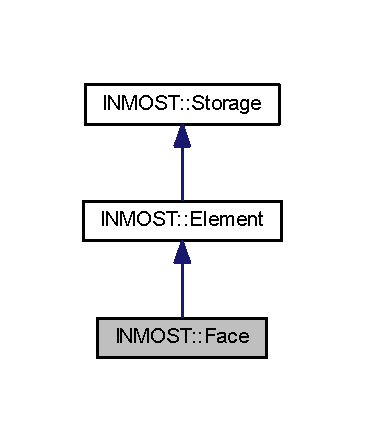
\includegraphics[width=175pt]{classINMOST_1_1Face__inherit__graph}
\end{center}
\end{figure}


Collaboration diagram for I\-N\-M\-O\-S\-T\-:\-:Face\-:
\nopagebreak
\begin{figure}[H]
\begin{center}
\leavevmode
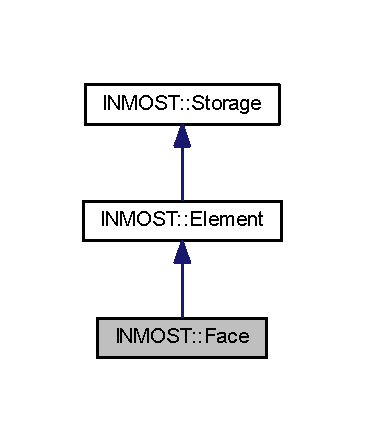
\includegraphics[width=175pt]{classINMOST_1_1Face__coll__graph}
\end{center}
\end{figure}
\subsection*{Public Member Functions}
\begin{DoxyCompactItemize}
\item 
\hypertarget{classINMOST_1_1Face_a53034833744bd5d87a3ae6d933651145}{{\bfseries Face} (const \hyperlink{classINMOST_1_1Face}{Face} \&other)}\label{classINMOST_1_1Face_a53034833744bd5d87a3ae6d933651145}

\item 
\hypertarget{classINMOST_1_1Face_acb563a6337c86a4cf94a710e4e999713}{{\bfseries Face} (\hyperlink{classINMOST_1_1Mesh}{Mesh} $\ast$m, Handle\-Type h)}\label{classINMOST_1_1Face_acb563a6337c86a4cf94a710e4e999713}

\item 
\hypertarget{classINMOST_1_1Face_a9e972af360efe84b5024c5462b6febc8}{{\bfseries Face} (\hyperlink{classINMOST_1_1Mesh}{Mesh} $\ast$m, Handle\-Type $\ast$h)}\label{classINMOST_1_1Face_a9e972af360efe84b5024c5462b6febc8}

\item 
\hypertarget{classINMOST_1_1Face_a6a6f3c1fbe976e4190b65ef840761963}{\hyperlink{classINMOST_1_1Face}{Face} \& {\bfseries operator=} (\hyperlink{classINMOST_1_1Face}{Face} const \&other)}\label{classINMOST_1_1Face_a6a6f3c1fbe976e4190b65ef840761963}

\item 
\hypertarget{classINMOST_1_1Face_a230d80b0f802ce707bba105de43b9245}{\hyperlink{classINMOST_1_1Face}{Face} $\ast$ {\bfseries operator-\/$>$} ()}\label{classINMOST_1_1Face_a230d80b0f802ce707bba105de43b9245}

\item 
\hypertarget{classINMOST_1_1Face_aab957de5751d121cd10b1d397bd97986}{const \hyperlink{classINMOST_1_1Face}{Face} $\ast$ {\bfseries operator-\/$>$} () const }\label{classINMOST_1_1Face_aab957de5751d121cd10b1d397bd97986}

\item 
\hypertarget{classINMOST_1_1Face_a9048c2c08180e0e4808a2f3f6ea1c144}{\hyperlink{classINMOST_1_1Face}{Face} \& {\bfseries self} ()}\label{classINMOST_1_1Face_a9048c2c08180e0e4808a2f3f6ea1c144}

\item 
\hypertarget{classINMOST_1_1Face_a4485c40611961b928f525a729990c65a}{const \hyperlink{classINMOST_1_1Face}{Face} \& {\bfseries self} () const }\label{classINMOST_1_1Face_a4485c40611961b928f525a729990c65a}

\item 
\hyperlink{classINMOST_1_1ElementArray}{Element\-Array}$<$ \hyperlink{classINMOST_1_1Node}{Node} $>$ \hyperlink{classINMOST_1_1Face_a102ef5504795e2b3607093071259397e}{get\-Nodes} () const 
\begin{DoxyCompactList}\small\item\em Retrieve all the nodes of the element. \end{DoxyCompactList}\item 
\hyperlink{classINMOST_1_1ElementArray}{Element\-Array}$<$ \hyperlink{classINMOST_1_1Edge}{Edge} $>$ \hyperlink{classINMOST_1_1Face_aaf5b6793bec15dec905f198b2c46c912}{get\-Edges} () const 
\begin{DoxyCompactList}\small\item\em Retrieve all the edges of the element. \end{DoxyCompactList}\item 
\hyperlink{classINMOST_1_1ElementArray}{Element\-Array}$<$ \hyperlink{classINMOST_1_1Cell}{Cell} $>$ \hyperlink{classINMOST_1_1Face_a4c1a9d6300f0b8da3032753380a1846c}{get\-Cells} () const 
\begin{DoxyCompactList}\small\item\em Return all the cells of the element. \end{DoxyCompactList}\item 
\hypertarget{classINMOST_1_1Face_adfac7ba1a6dd2db5b2ef8fedee9663ed}{\hyperlink{classINMOST_1_1ElementArray}{Element\-Array}$<$ \hyperlink{classINMOST_1_1Node}{Node} $>$ {\bfseries get\-Nodes} (Marker\-Type mask, bool invert\-\_\-mask=false) const }\label{classINMOST_1_1Face_adfac7ba1a6dd2db5b2ef8fedee9663ed}

\item 
\hypertarget{classINMOST_1_1Face_ac8f705c1ac68aee4b2406123df50120a}{\hyperlink{classINMOST_1_1ElementArray}{Element\-Array}$<$ \hyperlink{classINMOST_1_1Edge}{Edge} $>$ {\bfseries get\-Edges} (Marker\-Type mask, bool invert\-\_\-mask=false) const }\label{classINMOST_1_1Face_ac8f705c1ac68aee4b2406123df50120a}

\item 
\hypertarget{classINMOST_1_1Face_a757b996ae899ef89a13fb076a34c0528}{\hyperlink{classINMOST_1_1ElementArray}{Element\-Array}$<$ \hyperlink{classINMOST_1_1Cell}{Cell} $>$ {\bfseries get\-Cells} (Marker\-Type mask, bool invert\-\_\-mask=false) const }\label{classINMOST_1_1Face_a757b996ae899ef89a13fb076a34c0528}

\item 
\hypertarget{classINMOST_1_1Face_a944a85186680ca168a45e323ad719d70}{\hyperlink{classINMOST_1_1Node}{Node} {\bfseries get\-Beg} () const }\label{classINMOST_1_1Face_a944a85186680ca168a45e323ad719d70}

\item 
\hypertarget{classINMOST_1_1Face_adb70180c6aad1893e2fe754a8d88e170}{\hyperlink{classINMOST_1_1Node}{Node} {\bfseries get\-End} () const }\label{classINMOST_1_1Face_adb70180c6aad1893e2fe754a8d88e170}

\item 
\hyperlink{classINMOST_1_1Cell}{Cell} \hyperlink{classINMOST_1_1Face_a343f374489d97e5cc41e392f1fd29eea}{Back\-Cell} () const 
\begin{DoxyCompactList}\small\item\em Retrieve the cell for which the normal points outwards. \end{DoxyCompactList}\item 
\hyperlink{classINMOST_1_1Cell}{Cell} \hyperlink{classINMOST_1_1Face_a31695655cabb60aef6e7048d175cd0de}{Front\-Cell} () const 
\begin{DoxyCompactList}\small\item\em Retrieve the cell for which the normal points inwards. \end{DoxyCompactList}\item 
\hypertarget{classINMOST_1_1Face_ac8e9ea9a38d8c5732c3618b21ec6c346}{bool {\bfseries Face\-Oriented\-Outside} (\hyperlink{classINMOST_1_1Cell}{Cell} c) const }\label{classINMOST_1_1Face_ac8e9ea9a38d8c5732c3618b21ec6c346}

\item 
\hypertarget{classINMOST_1_1Face_a0e621e47a29cba52983e2dbe4b5595f5}{void {\bfseries Reorder\-Edges} () const }\label{classINMOST_1_1Face_a0e621e47a29cba52983e2dbe4b5595f5}

\item 
\hypertarget{classINMOST_1_1Face_afe466ba6d89813531fa7d8bcda47c22a}{bool {\bfseries Check\-Edge\-Order} () const }\label{classINMOST_1_1Face_afe466ba6d89813531fa7d8bcda47c22a}

\item 
\hypertarget{classINMOST_1_1Face_a7c197d0d9d1da8b39815ec8193470d55}{bool {\bfseries Fix\-Edge\-Order} () const }\label{classINMOST_1_1Face_a7c197d0d9d1da8b39815ec8193470d55}

\item 
\hypertarget{classINMOST_1_1Face_afc7145b4345851c8b63d4cb1fb3f7fb8}{void {\bfseries Swap\-Cells} ()}\label{classINMOST_1_1Face_afc7145b4345851c8b63d4cb1fb3f7fb8}

\item 
\hypertarget{classINMOST_1_1Face_ae64a118505766e645f81a608d1bca9b3}{\hyperlink{classINMOST_1_1Storage_a853346784b4a5822a7fac54d8f10f805}{Storage\-::real} {\bfseries Area} () const }\label{classINMOST_1_1Face_ae64a118505766e645f81a608d1bca9b3}

\item 
\hypertarget{classINMOST_1_1Face_a1d88c443096cda59520e89857b8338fa}{void {\bfseries Normal} (\hyperlink{classINMOST_1_1Storage_a853346784b4a5822a7fac54d8f10f805}{real} $\ast$nrm) const }\label{classINMOST_1_1Face_a1d88c443096cda59520e89857b8338fa}

\item 
\hypertarget{classINMOST_1_1Face_a1dd3d4570f8d22104b606094a5c1c983}{void {\bfseries Unit\-Normal} (\hyperlink{classINMOST_1_1Storage_a853346784b4a5822a7fac54d8f10f805}{real} $\ast$nrm) const }\label{classINMOST_1_1Face_a1dd3d4570f8d22104b606094a5c1c983}

\item 
\hypertarget{classINMOST_1_1Face_acc9ff2f465808c7da9b11fe2bfe05e68}{void {\bfseries Oriented\-Normal} (\hyperlink{classINMOST_1_1Cell}{Cell} c, \hyperlink{classINMOST_1_1Storage_a853346784b4a5822a7fac54d8f10f805}{real} $\ast$nrm) const }\label{classINMOST_1_1Face_acc9ff2f465808c7da9b11fe2bfe05e68}

\item 
\hypertarget{classINMOST_1_1Face_a2a624f1435b028243efc9ab1dbbb45d2}{void {\bfseries Oriented\-Unit\-Normal} (\hyperlink{classINMOST_1_1Cell}{Cell} c, \hyperlink{classINMOST_1_1Storage_a853346784b4a5822a7fac54d8f10f805}{real} $\ast$nrm) const }\label{classINMOST_1_1Face_a2a624f1435b028243efc9ab1dbbb45d2}

\item 
\hypertarget{classINMOST_1_1Face_a92e3c5875775427822426b6bc891a019}{bool {\bfseries Fix\-Normal\-Orientation} () const }\label{classINMOST_1_1Face_a92e3c5875775427822426b6bc891a019}

\item 
\hypertarget{classINMOST_1_1Face_a04e7a630eee6a9154c74254a7c08bac9}{bool {\bfseries Check\-Normal\-Orientation} () const }\label{classINMOST_1_1Face_a04e7a630eee6a9154c74254a7c08bac9}

\item 
\hypertarget{classINMOST_1_1Face_ab825faac44428f15c5fd03ffbe45df27}{bool {\bfseries Closure} () const }\label{classINMOST_1_1Face_ab825faac44428f15c5fd03ffbe45df27}

\end{DoxyCompactItemize}
\subsection*{Static Public Member Functions}
\begin{DoxyCompactItemize}
\item 
\hypertarget{classINMOST_1_1Face_a0da6611e6eb20b2dd0f7e01617431c60}{static \hyperlink{classINMOST_1_1Face}{Face} {\bfseries Unite\-Faces} (\hyperlink{classINMOST_1_1ElementArray}{Element\-Array}$<$ \hyperlink{classINMOST_1_1Face}{Face} $>$ \&faces, Marker\-Type del\-\_\-protect)}\label{classINMOST_1_1Face_a0da6611e6eb20b2dd0f7e01617431c60}

\item 
\hypertarget{classINMOST_1_1Face_ad1d2622f4dda9c86a9c2183364afd50c}{static bool {\bfseries Test\-Unite\-Faces} (const \hyperlink{classINMOST_1_1ElementArray}{Element\-Array}$<$ \hyperlink{classINMOST_1_1Face}{Face} $>$ \&faces, Marker\-Type del\-\_\-protect)}\label{classINMOST_1_1Face_ad1d2622f4dda9c86a9c2183364afd50c}

\item 
\hypertarget{classINMOST_1_1Face_aef8f16b0fcae39923a0cb7194bfce778}{static \hyperlink{classINMOST_1_1ElementArray}{Element\-Array}$<$ \hyperlink{classINMOST_1_1Face}{Face} $>$ {\bfseries Split\-Face} (\hyperlink{classINMOST_1_1Face}{Face} face, const \hyperlink{classINMOST_1_1ElementArray}{Element\-Array}$<$ \hyperlink{classINMOST_1_1Edge}{Edge} $>$ \&edges, Marker\-Type del\-\_\-protect)}\label{classINMOST_1_1Face_aef8f16b0fcae39923a0cb7194bfce778}

\item 
\hypertarget{classINMOST_1_1Face_a44249a6794cf295d698027b6a52c91a8}{static bool {\bfseries Test\-Split\-Face} (\hyperlink{classINMOST_1_1Face}{Face} face, const \hyperlink{classINMOST_1_1ElementArray}{Element\-Array}$<$ \hyperlink{classINMOST_1_1Edge}{Edge} $>$ \&edges, Marker\-Type del\-\_\-protect)}\label{classINMOST_1_1Face_a44249a6794cf295d698027b6a52c91a8}

\end{DoxyCompactItemize}
\subsection*{Additional Inherited Members}


\subsection{Member Function Documentation}
\hypertarget{classINMOST_1_1Face_a343f374489d97e5cc41e392f1fd29eea}{\index{I\-N\-M\-O\-S\-T\-::\-Face@{I\-N\-M\-O\-S\-T\-::\-Face}!Back\-Cell@{Back\-Cell}}
\index{Back\-Cell@{Back\-Cell}!INMOST::Face@{I\-N\-M\-O\-S\-T\-::\-Face}}
\subsubsection[{Back\-Cell}]{\setlength{\rightskip}{0pt plus 5cm}{\bf Cell} I\-N\-M\-O\-S\-T\-::\-Face\-::\-Back\-Cell (
\begin{DoxyParamCaption}
{}
\end{DoxyParamCaption}
) const}}\label{classINMOST_1_1Face_a343f374489d97e5cc41e392f1fd29eea}


Retrieve the cell for which the normal points outwards. 

Depending on the grid construction the normal may incorrectly point inwards. You can resolve this situation by Face\-::\-Fix\-Normal\-Orientation. \begin{DoxyReturn}{Returns}
the cell for which normal points outwards. 
\end{DoxyReturn}
\begin{DoxySeeAlso}{See Also}
Face\-::\-Fix\-Normal\-Orientation 
\end{DoxySeeAlso}
\hypertarget{classINMOST_1_1Face_a31695655cabb60aef6e7048d175cd0de}{\index{I\-N\-M\-O\-S\-T\-::\-Face@{I\-N\-M\-O\-S\-T\-::\-Face}!Front\-Cell@{Front\-Cell}}
\index{Front\-Cell@{Front\-Cell}!INMOST::Face@{I\-N\-M\-O\-S\-T\-::\-Face}}
\subsubsection[{Front\-Cell}]{\setlength{\rightskip}{0pt plus 5cm}{\bf Cell} I\-N\-M\-O\-S\-T\-::\-Face\-::\-Front\-Cell (
\begin{DoxyParamCaption}
{}
\end{DoxyParamCaption}
) const}}\label{classINMOST_1_1Face_a31695655cabb60aef6e7048d175cd0de}


Retrieve the cell for which the normal points inwards. 

Depending on the grid construction the normal may incorrectly point outwards. You can resolve this situation by Face\-::\-Fix\-Normal\-Orientation. \begin{DoxyReturn}{Returns}
the cell for which normal points inwards. 
\end{DoxyReturn}
\begin{DoxySeeAlso}{See Also}
Face\-::\-Fix\-Normal\-Orientation 
\end{DoxySeeAlso}
\hypertarget{classINMOST_1_1Face_a4c1a9d6300f0b8da3032753380a1846c}{\index{I\-N\-M\-O\-S\-T\-::\-Face@{I\-N\-M\-O\-S\-T\-::\-Face}!get\-Cells@{get\-Cells}}
\index{get\-Cells@{get\-Cells}!INMOST::Face@{I\-N\-M\-O\-S\-T\-::\-Face}}
\subsubsection[{get\-Cells}]{\setlength{\rightskip}{0pt plus 5cm}{\bf Element\-Array}$<${\bf Cell}$>$ I\-N\-M\-O\-S\-T\-::\-Face\-::get\-Cells (
\begin{DoxyParamCaption}
{}
\end{DoxyParamCaption}
) const\hspace{0.3cm}{\ttfamily [virtual]}}}\label{classINMOST_1_1Face_a4c1a9d6300f0b8da3032753380a1846c}


Return all the cells of the element. 

For a node returns unordered set of cells.

For an edge returns unordered set of cells.

For a face returns a pair of cells. In the case Face\-::\-Check\-Normal\-Orientation returns true then the normal points from the first cell to the second and in oppisite direction otherwise.

For a cell returns itself.

\begin{DoxyReturn}{Returns}
array of elements 
\end{DoxyReturn}
\begin{DoxySeeAlso}{See Also}
Face\-::\-Face\-Oriented\-Outside 
\end{DoxySeeAlso}


Reimplemented from \hyperlink{classINMOST_1_1Element_aa90ec6b1e297fb9c1322b5558ccb7e2d}{I\-N\-M\-O\-S\-T\-::\-Element}.

\hypertarget{classINMOST_1_1Face_aaf5b6793bec15dec905f198b2c46c912}{\index{I\-N\-M\-O\-S\-T\-::\-Face@{I\-N\-M\-O\-S\-T\-::\-Face}!get\-Edges@{get\-Edges}}
\index{get\-Edges@{get\-Edges}!INMOST::Face@{I\-N\-M\-O\-S\-T\-::\-Face}}
\subsubsection[{get\-Edges}]{\setlength{\rightskip}{0pt plus 5cm}{\bf Element\-Array}$<${\bf Edge}$>$ I\-N\-M\-O\-S\-T\-::\-Face\-::get\-Edges (
\begin{DoxyParamCaption}
{}
\end{DoxyParamCaption}
) const\hspace{0.3cm}{\ttfamily [virtual]}}}\label{classINMOST_1_1Face_aaf5b6793bec15dec905f198b2c46c912}


Retrieve all the edges of the element. 

For a node returns unordered set of edges.

For an edge returns itself.

For a face returns ordered set of edges.

For a cell returns unordered set of edges.

\begin{DoxyReturn}{Returns}
array of elements 
\end{DoxyReturn}


Reimplemented from \hyperlink{classINMOST_1_1Element_a3ba56a19eeeb283864a006b0744fac4e}{I\-N\-M\-O\-S\-T\-::\-Element}.

\hypertarget{classINMOST_1_1Face_a102ef5504795e2b3607093071259397e}{\index{I\-N\-M\-O\-S\-T\-::\-Face@{I\-N\-M\-O\-S\-T\-::\-Face}!get\-Nodes@{get\-Nodes}}
\index{get\-Nodes@{get\-Nodes}!INMOST::Face@{I\-N\-M\-O\-S\-T\-::\-Face}}
\subsubsection[{get\-Nodes}]{\setlength{\rightskip}{0pt plus 5cm}{\bf Element\-Array}$<${\bf Node}$>$ I\-N\-M\-O\-S\-T\-::\-Face\-::get\-Nodes (
\begin{DoxyParamCaption}
{}
\end{DoxyParamCaption}
) const\hspace{0.3cm}{\ttfamily [virtual]}}}\label{classINMOST_1_1Face_a102ef5504795e2b3607093071259397e}


Retrieve all the nodes of the element. 

For a node returns itself.

For an edge returns ordered pair of nodes. The order of nodes in the edge is preserved from the first creation.

For a face returns ordered set of nodes. In the case Face\-::\-Check\-Normal\-Orientation returns true the order of nodes will follow right hand side rule with respect to normal vector, otherwise it follows left hand side rule with respect to normal vector.

For a cell returns the same order that was provided through suggest\-\_\-nodes\-\_\-oreder in Mesh\-::\-Create\-Cell. In the case suggest\-\_\-nodes\-\_\-order was not provided, the order of nodes follows V\-T\-K format for known types of elements such as Element\-::\-Tet, Element\-::\-Prism, Element\-::\-Hex, Element\-::\-Pyramid. For a general polyhedron the order is unspecified.

\begin{DoxyReturn}{Returns}
array of elements 
\end{DoxyReturn}
\begin{DoxySeeAlso}{See Also}
Face\-::\-Check\-Normal\-Orientation 

Face\-::\-Face\-Oriented\-Outside 
\end{DoxySeeAlso}


Reimplemented from \hyperlink{classINMOST_1_1Element_a00696ff8cd77491e1c4307cae166e92d}{I\-N\-M\-O\-S\-T\-::\-Element}.



The documentation for this class was generated from the following file\-:\begin{DoxyCompactItemize}
\item 
inmost\-\_\-mesh.\-h\end{DoxyCompactItemize}

\hypertarget{classINMOST_1_1Mesh_1_1GlobalIDComparator}{\section{I\-N\-M\-O\-S\-T\-:\-:Mesh\-:\-:Global\-I\-D\-Comparator Class Reference}
\label{classINMOST_1_1Mesh_1_1GlobalIDComparator}\index{I\-N\-M\-O\-S\-T\-::\-Mesh\-::\-Global\-I\-D\-Comparator@{I\-N\-M\-O\-S\-T\-::\-Mesh\-::\-Global\-I\-D\-Comparator}}
}
\subsection*{Public Member Functions}
\begin{DoxyCompactItemize}
\item 
\hypertarget{classINMOST_1_1Mesh_1_1GlobalIDComparator_a554e10d8c822c38589546e5272626fbb}{{\bfseries Global\-I\-D\-Comparator} (\hyperlink{classINMOST_1_1Mesh}{Mesh} $\ast$m)}\label{classINMOST_1_1Mesh_1_1GlobalIDComparator_a554e10d8c822c38589546e5272626fbb}

\item 
\hypertarget{classINMOST_1_1Mesh_1_1GlobalIDComparator_ae23c9b0bcef351c6160b302883e16bd7}{{\bfseries Global\-I\-D\-Comparator} (const \hyperlink{classINMOST_1_1Mesh_1_1GlobalIDComparator}{Global\-I\-D\-Comparator} \&other)}\label{classINMOST_1_1Mesh_1_1GlobalIDComparator_ae23c9b0bcef351c6160b302883e16bd7}

\item 
\hypertarget{classINMOST_1_1Mesh_1_1GlobalIDComparator_a01646d1493a93ed524f8f7931f5ff820}{\hyperlink{classINMOST_1_1Mesh_1_1GlobalIDComparator}{Global\-I\-D\-Comparator} \& {\bfseries operator=} (\hyperlink{classINMOST_1_1Mesh_1_1GlobalIDComparator}{Global\-I\-D\-Comparator} const \&other)}\label{classINMOST_1_1Mesh_1_1GlobalIDComparator_a01646d1493a93ed524f8f7931f5ff820}

\item 
\hypertarget{classINMOST_1_1Mesh_1_1GlobalIDComparator_ac382eb1939cb5099bafb7fca4b081e3c}{bool {\bfseries operator()} (Handle\-Type a, Handle\-Type b) const }\label{classINMOST_1_1Mesh_1_1GlobalIDComparator_ac382eb1939cb5099bafb7fca4b081e3c}

\item 
\hypertarget{classINMOST_1_1Mesh_1_1GlobalIDComparator_a43c30f59baa22cd86ad4ac31a9bbeef6}{bool {\bfseries operator()} (Handle\-Type a, \hyperlink{classINMOST_1_1Storage_aec96942bc647417a801e2895b45964d2}{integer} gid) const }\label{classINMOST_1_1Mesh_1_1GlobalIDComparator_a43c30f59baa22cd86ad4ac31a9bbeef6}

\end{DoxyCompactItemize}


The documentation for this class was generated from the following file\-:\begin{DoxyCompactItemize}
\item 
inmost\-\_\-mesh.\-h\end{DoxyCompactItemize}

\hypertarget{classINMOST_1_1Mesh_1_1IerarhyComparator}{\section{I\-N\-M\-O\-S\-T\-:\-:Mesh\-:\-:Ierarhy\-Comparator Class Reference}
\label{classINMOST_1_1Mesh_1_1IerarhyComparator}\index{I\-N\-M\-O\-S\-T\-::\-Mesh\-::\-Ierarhy\-Comparator@{I\-N\-M\-O\-S\-T\-::\-Mesh\-::\-Ierarhy\-Comparator}}
}
\subsection*{Public Member Functions}
\begin{DoxyCompactItemize}
\item 
\hypertarget{classINMOST_1_1Mesh_1_1IerarhyComparator_aa1aace576057479c4c766a80c3f1c05b}{{\bfseries Ierarhy\-Comparator} (\hyperlink{classINMOST_1_1Mesh}{Mesh} $\ast$m)}\label{classINMOST_1_1Mesh_1_1IerarhyComparator_aa1aace576057479c4c766a80c3f1c05b}

\item 
\hypertarget{classINMOST_1_1Mesh_1_1IerarhyComparator_a26ad54ab39301f8adc84b42b744719e8}{{\bfseries Ierarhy\-Comparator} (const \hyperlink{classINMOST_1_1Mesh_1_1IerarhyComparator}{Ierarhy\-Comparator} \&other)}\label{classINMOST_1_1Mesh_1_1IerarhyComparator_a26ad54ab39301f8adc84b42b744719e8}

\item 
\hypertarget{classINMOST_1_1Mesh_1_1IerarhyComparator_a7b467f71e87b62ba9440cfbe3cbc1bcc}{\hyperlink{classINMOST_1_1Mesh_1_1IerarhyComparator}{Ierarhy\-Comparator} \& {\bfseries operator=} (\hyperlink{classINMOST_1_1Mesh_1_1IerarhyComparator}{Ierarhy\-Comparator} const \&other)}\label{classINMOST_1_1Mesh_1_1IerarhyComparator_a7b467f71e87b62ba9440cfbe3cbc1bcc}

\item 
\hypertarget{classINMOST_1_1Mesh_1_1IerarhyComparator_a586cefae2bce4e04fedbf7e767eff555}{int {\bfseries Compare\-Nodes} (Handle\-Type a, Handle\-Type b) const }\label{classINMOST_1_1Mesh_1_1IerarhyComparator_a586cefae2bce4e04fedbf7e767eff555}

\item 
\hypertarget{classINMOST_1_1Mesh_1_1IerarhyComparator_ad8ec126d5fa88d41da914c31e9b8fe81}{int {\bfseries Compare\-Elements} (Handle\-Type a, Handle\-Type b) const }\label{classINMOST_1_1Mesh_1_1IerarhyComparator_ad8ec126d5fa88d41da914c31e9b8fe81}

\item 
\hypertarget{classINMOST_1_1Mesh_1_1IerarhyComparator_ad98a25c830e36605854a0cfb3415c761}{bool {\bfseries operator()} (Handle\-Type a, Handle\-Type b) const }\label{classINMOST_1_1Mesh_1_1IerarhyComparator_ad98a25c830e36605854a0cfb3415c761}

\end{DoxyCompactItemize}


The documentation for this class was generated from the following file\-:\begin{DoxyCompactItemize}
\item 
inmost\-\_\-mesh.\-h\end{DoxyCompactItemize}

\hypertarget{classINMOST_1_1Mesh_1_1IntegerComparator}{\section{I\-N\-M\-O\-S\-T\-:\-:Mesh\-:\-:Integer\-Comparator Class Reference}
\label{classINMOST_1_1Mesh_1_1IntegerComparator}\index{I\-N\-M\-O\-S\-T\-::\-Mesh\-::\-Integer\-Comparator@{I\-N\-M\-O\-S\-T\-::\-Mesh\-::\-Integer\-Comparator}}
}
\subsection*{Public Member Functions}
\begin{DoxyCompactItemize}
\item 
\hypertarget{classINMOST_1_1Mesh_1_1IntegerComparator_a1a7c2ba35315439921b6a51a2db7a58f}{{\bfseries Integer\-Comparator} (\hyperlink{classINMOST_1_1Mesh}{Mesh} $\ast$m, \hyperlink{classINMOST_1_1Tag}{Tag} t)}\label{classINMOST_1_1Mesh_1_1IntegerComparator_a1a7c2ba35315439921b6a51a2db7a58f}

\item 
\hypertarget{classINMOST_1_1Mesh_1_1IntegerComparator_a22316d8856c0752c89d4fc56cd605da5}{{\bfseries Integer\-Comparator} (const \hyperlink{classINMOST_1_1Mesh_1_1IntegerComparator}{Integer\-Comparator} \&other)}\label{classINMOST_1_1Mesh_1_1IntegerComparator_a22316d8856c0752c89d4fc56cd605da5}

\item 
\hypertarget{classINMOST_1_1Mesh_1_1IntegerComparator_a32b1d4ade571c1da94618f2e3fdbc7a4}{\hyperlink{classINMOST_1_1Mesh_1_1IntegerComparator}{Integer\-Comparator} \& {\bfseries operator=} (\hyperlink{classINMOST_1_1Mesh_1_1IntegerComparator}{Integer\-Comparator} const \&other)}\label{classINMOST_1_1Mesh_1_1IntegerComparator_a32b1d4ade571c1da94618f2e3fdbc7a4}

\item 
\hypertarget{classINMOST_1_1Mesh_1_1IntegerComparator_a521ea8d9df71795f037272d6a45523de}{bool {\bfseries operator()} (Handle\-Type a, Handle\-Type b) const }\label{classINMOST_1_1Mesh_1_1IntegerComparator_a521ea8d9df71795f037272d6a45523de}

\item 
\hypertarget{classINMOST_1_1Mesh_1_1IntegerComparator_a4e34a23fd113587793d17bdb3ff1b329}{bool {\bfseries operator()} (Handle\-Type a, \hyperlink{classINMOST_1_1Storage_aec96942bc647417a801e2895b45964d2}{integer} b) const }\label{classINMOST_1_1Mesh_1_1IntegerComparator_a4e34a23fd113587793d17bdb3ff1b329}

\end{DoxyCompactItemize}


The documentation for this class was generated from the following file\-:\begin{DoxyCompactItemize}
\item 
inmost\-\_\-mesh.\-h\end{DoxyCompactItemize}

\hypertarget{classINMOST_1_1Mesh_1_1IntegerDFComparator}{\section{I\-N\-M\-O\-S\-T\-:\-:Mesh\-:\-:Integer\-D\-F\-Comparator Class Reference}
\label{classINMOST_1_1Mesh_1_1IntegerDFComparator}\index{I\-N\-M\-O\-S\-T\-::\-Mesh\-::\-Integer\-D\-F\-Comparator@{I\-N\-M\-O\-S\-T\-::\-Mesh\-::\-Integer\-D\-F\-Comparator}}
}
\subsection*{Public Member Functions}
\begin{DoxyCompactItemize}
\item 
\hypertarget{classINMOST_1_1Mesh_1_1IntegerDFComparator_a57bee2323b04b1891182e8bbfcb8063a}{{\bfseries Integer\-D\-F\-Comparator} (\hyperlink{classINMOST_1_1Mesh}{Mesh} $\ast$m, \hyperlink{classINMOST_1_1Tag}{Tag} t)}\label{classINMOST_1_1Mesh_1_1IntegerDFComparator_a57bee2323b04b1891182e8bbfcb8063a}

\item 
\hypertarget{classINMOST_1_1Mesh_1_1IntegerDFComparator_a26ffe919a208756099d6e335050122ff}{{\bfseries Integer\-D\-F\-Comparator} (const \hyperlink{classINMOST_1_1Mesh_1_1IntegerDFComparator}{Integer\-D\-F\-Comparator} \&other)}\label{classINMOST_1_1Mesh_1_1IntegerDFComparator_a26ffe919a208756099d6e335050122ff}

\item 
\hypertarget{classINMOST_1_1Mesh_1_1IntegerDFComparator_ad25cdf693d82edbce170a7aa114bb881}{\hyperlink{classINMOST_1_1Mesh_1_1IntegerDFComparator}{Integer\-D\-F\-Comparator} \& {\bfseries operator=} (\hyperlink{classINMOST_1_1Mesh_1_1IntegerDFComparator}{Integer\-D\-F\-Comparator} const \&other)}\label{classINMOST_1_1Mesh_1_1IntegerDFComparator_ad25cdf693d82edbce170a7aa114bb881}

\item 
\hypertarget{classINMOST_1_1Mesh_1_1IntegerDFComparator_afff0d1793113eb0d1a8f90e98d5c118a}{bool {\bfseries operator()} (Handle\-Type a, Handle\-Type b) const }\label{classINMOST_1_1Mesh_1_1IntegerDFComparator_afff0d1793113eb0d1a8f90e98d5c118a}

\item 
\hypertarget{classINMOST_1_1Mesh_1_1IntegerDFComparator_a0d9e6ecec378cedd4ae3cca369da852e}{bool {\bfseries operator()} (Handle\-Type a, \hyperlink{classINMOST_1_1Storage_aec96942bc647417a801e2895b45964d2}{integer} b) const }\label{classINMOST_1_1Mesh_1_1IntegerDFComparator_a0d9e6ecec378cedd4ae3cca369da852e}

\end{DoxyCompactItemize}


The documentation for this class was generated from the following file\-:\begin{DoxyCompactItemize}
\item 
inmost\-\_\-mesh.\-h\end{DoxyCompactItemize}

\hypertarget{classINMOST_1_1Storage_1_1reference__array_1_1iterator}{\section{I\-N\-M\-O\-S\-T\-:\-:Storage\-:\-:reference\-\_\-array\-:\-:iterator Class Reference}
\label{classINMOST_1_1Storage_1_1reference__array_1_1iterator}\index{I\-N\-M\-O\-S\-T\-::\-Storage\-::reference\-\_\-array\-::iterator@{I\-N\-M\-O\-S\-T\-::\-Storage\-::reference\-\_\-array\-::iterator}}
}


Inheritance diagram for I\-N\-M\-O\-S\-T\-:\-:Storage\-:\-:reference\-\_\-array\-:\-:iterator\-:\nopagebreak
\begin{figure}[H]
\begin{center}
\leavevmode
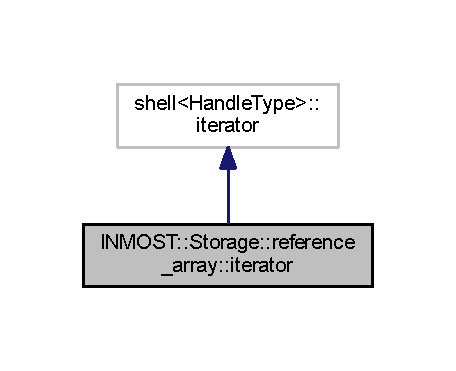
\includegraphics[width=219pt]{classINMOST_1_1Storage_1_1reference__array_1_1iterator__inherit__graph}
\end{center}
\end{figure}


Collaboration diagram for I\-N\-M\-O\-S\-T\-:\-:Storage\-:\-:reference\-\_\-array\-:\-:iterator\-:\nopagebreak
\begin{figure}[H]
\begin{center}
\leavevmode
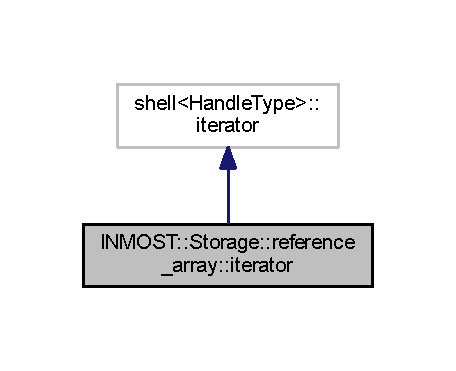
\includegraphics[width=219pt]{classINMOST_1_1Storage_1_1reference__array_1_1iterator__coll__graph}
\end{center}
\end{figure}
\subsection*{Public Member Functions}
\begin{DoxyCompactItemize}
\item 
\hypertarget{classINMOST_1_1Storage_1_1reference__array_1_1iterator_a023bd432b920c75c4eabea619976dcb5}{{\bfseries iterator} (\hyperlink{classINMOST_1_1Mesh}{Mesh} $\ast$m, const shell$<$ Handle\-Type $>$\-::\hyperlink{classINMOST_1_1Storage_1_1reference__array_1_1iterator}{iterator} \&other)}\label{classINMOST_1_1Storage_1_1reference__array_1_1iterator_a023bd432b920c75c4eabea619976dcb5}

\item 
\hypertarget{classINMOST_1_1Storage_1_1reference__array_1_1iterator_a3d4d4dbcc15b4f1c00235d10ddeabc4d}{{\bfseries iterator} (const \hyperlink{classINMOST_1_1Storage_1_1reference__array_1_1iterator}{iterator} \&other)}\label{classINMOST_1_1Storage_1_1reference__array_1_1iterator_a3d4d4dbcc15b4f1c00235d10ddeabc4d}

\item 
\hypertarget{classINMOST_1_1Storage_1_1reference__array_1_1iterator_adf41f797a07ea1af42d64e5b3ef850bd}{\hyperlink{classINMOST_1_1Storage_1_1reference__array_1_1iterator}{iterator} \& {\bfseries operator=} (\hyperlink{classINMOST_1_1Storage_1_1reference__array_1_1iterator}{iterator} const \&other)}\label{classINMOST_1_1Storage_1_1reference__array_1_1iterator_adf41f797a07ea1af42d64e5b3ef850bd}

\item 
\hypertarget{classINMOST_1_1Storage_1_1reference__array_1_1iterator_aa1d37095116283ec5f8ce192abac1c23}{\hyperlink{classINMOST_1_1Storage_1_1reference__array_1_1iterator}{iterator} \& {\bfseries operator++} ()}\label{classINMOST_1_1Storage_1_1reference__array_1_1iterator_aa1d37095116283ec5f8ce192abac1c23}

\item 
\hypertarget{classINMOST_1_1Storage_1_1reference__array_1_1iterator_a8997a8344242c73e61d0c247c876bb12}{\hyperlink{classINMOST_1_1Storage_1_1reference__array_1_1iterator}{iterator} {\bfseries operator++} (int)}\label{classINMOST_1_1Storage_1_1reference__array_1_1iterator_a8997a8344242c73e61d0c247c876bb12}

\item 
\hypertarget{classINMOST_1_1Storage_1_1reference__array_1_1iterator_af2ad0f65f68fc3b3c15c1de83bf550b8}{\hyperlink{classINMOST_1_1Storage_1_1reference__array_1_1iterator}{iterator} \& {\bfseries operator-\/-\/} ()}\label{classINMOST_1_1Storage_1_1reference__array_1_1iterator_af2ad0f65f68fc3b3c15c1de83bf550b8}

\item 
\hypertarget{classINMOST_1_1Storage_1_1reference__array_1_1iterator_afab74602f97345e820b091c02bb30005}{\hyperlink{classINMOST_1_1Storage_1_1reference__array_1_1iterator}{iterator} {\bfseries operator-\/-\/} (int)}\label{classINMOST_1_1Storage_1_1reference__array_1_1iterator_afab74602f97345e820b091c02bb30005}

\item 
\hypertarget{classINMOST_1_1Storage_1_1reference__array_1_1iterator_ab65dc146de15948c9665e22341606c17}{\hyperlink{classINMOST_1_1Element}{Element} {\bfseries operator-\/$>$} ()}\label{classINMOST_1_1Storage_1_1reference__array_1_1iterator_ab65dc146de15948c9665e22341606c17}

\end{DoxyCompactItemize}


The documentation for this class was generated from the following file\-:\begin{DoxyCompactItemize}
\item 
inmost\-\_\-mesh.\-h\end{DoxyCompactItemize}

\hypertarget{classINMOST_1_1ElementArray_1_1iterator}{\section{I\-N\-M\-O\-S\-T\-:\-:Element\-Array$<$ Storage\-Type $>$\-:\-:iterator Class Reference}
\label{classINMOST_1_1ElementArray_1_1iterator}\index{I\-N\-M\-O\-S\-T\-::\-Element\-Array$<$ Storage\-Type $>$\-::iterator@{I\-N\-M\-O\-S\-T\-::\-Element\-Array$<$ Storage\-Type $>$\-::iterator}}
}


Inheritance diagram for I\-N\-M\-O\-S\-T\-:\-:Element\-Array$<$ Storage\-Type $>$\-:\-:iterator\-:


Collaboration diagram for I\-N\-M\-O\-S\-T\-:\-:Element\-Array$<$ Storage\-Type $>$\-:\-:iterator\-:
\subsection*{Public Member Functions}
\begin{DoxyCompactItemize}
\item 
\hypertarget{classINMOST_1_1ElementArray_1_1iterator_a0d7c6fedcf18f246d2525278480ab202}{{\bfseries iterator} (\hyperlink{classINMOST_1_1Mesh}{Mesh} $\ast$m, const cont\-\_\-t\-::iterator \&other)}\label{classINMOST_1_1ElementArray_1_1iterator_a0d7c6fedcf18f246d2525278480ab202}

\item 
\hypertarget{classINMOST_1_1ElementArray_1_1iterator_af045c453415f0bdb6f66ecc275d68ad9}{{\bfseries iterator} (const \hyperlink{classINMOST_1_1ElementArray_1_1iterator}{iterator} \&other)}\label{classINMOST_1_1ElementArray_1_1iterator_af045c453415f0bdb6f66ecc275d68ad9}

\item 
\hypertarget{classINMOST_1_1ElementArray_1_1iterator_af94b1a080932ed4586be1333f254fa4e}{\hyperlink{classINMOST_1_1ElementArray_1_1iterator}{iterator} \& {\bfseries operator++} ()}\label{classINMOST_1_1ElementArray_1_1iterator_af94b1a080932ed4586be1333f254fa4e}

\item 
\hypertarget{classINMOST_1_1ElementArray_1_1iterator_acba25b30b678dd9b4b77a007481af687}{\hyperlink{classINMOST_1_1ElementArray_1_1iterator}{iterator} {\bfseries operator++} (int)}\label{classINMOST_1_1ElementArray_1_1iterator_acba25b30b678dd9b4b77a007481af687}

\item 
\hypertarget{classINMOST_1_1ElementArray_1_1iterator_a03175615f0565c3844375ec17ff69d31}{\hyperlink{classINMOST_1_1ElementArray_1_1iterator}{iterator} \& {\bfseries operator-\/-\/} ()}\label{classINMOST_1_1ElementArray_1_1iterator_a03175615f0565c3844375ec17ff69d31}

\item 
\hypertarget{classINMOST_1_1ElementArray_1_1iterator_ad0701ce77f9a5928bf121777e3ca5016}{\hyperlink{classINMOST_1_1ElementArray_1_1iterator}{iterator} {\bfseries operator-\/-\/} (int)}\label{classINMOST_1_1ElementArray_1_1iterator_ad0701ce77f9a5928bf121777e3ca5016}

\item 
\hypertarget{classINMOST_1_1ElementArray_1_1iterator_ae63a652dc0fa497c82e212990ce3de9d}{\hyperlink{classINMOST_1_1ElementArray_1_1iterator}{iterator} \& {\bfseries operator=} (\hyperlink{classINMOST_1_1ElementArray_1_1iterator}{iterator} const \&other)}\label{classINMOST_1_1ElementArray_1_1iterator_ae63a652dc0fa497c82e212990ce3de9d}

\item 
\hypertarget{classINMOST_1_1ElementArray_1_1iterator_afadc7da73e24f64fa4a14dbfe4c44f83}{Handle\-Type \& {\bfseries operator$\ast$} ()}\label{classINMOST_1_1ElementArray_1_1iterator_afadc7da73e24f64fa4a14dbfe4c44f83}

\item 
\hypertarget{classINMOST_1_1ElementArray_1_1iterator_a3168cfa2e3de18178aa55128df623f49}{Storage\-Type {\bfseries operator-\/$>$} ()}\label{classINMOST_1_1ElementArray_1_1iterator_a3168cfa2e3de18178aa55128df623f49}

\end{DoxyCompactItemize}


The documentation for this class was generated from the following file\-:\begin{DoxyCompactItemize}
\item 
inmost\-\_\-mesh.\-h\end{DoxyCompactItemize}

\hypertarget{classINMOST_1_1ElementSet_1_1iterator}{\section{I\-N\-M\-O\-S\-T\-:\-:Element\-Set\-:\-:iterator Class Reference}
\label{classINMOST_1_1ElementSet_1_1iterator}\index{I\-N\-M\-O\-S\-T\-::\-Element\-Set\-::iterator@{I\-N\-M\-O\-S\-T\-::\-Element\-Set\-::iterator}}
}
\subsection*{Public Types}
\begin{DoxyCompactItemize}
\item 
\hypertarget{classINMOST_1_1ElementSet_1_1iterator_af18ad6b71f7fd811618b1f1488827790}{typedef std\-::forward\-\_\-iterator\-\_\-tag {\bfseries iterator\-\_\-category}}\label{classINMOST_1_1ElementSet_1_1iterator_af18ad6b71f7fd811618b1f1488827790}

\end{DoxyCompactItemize}
\subsection*{Public Member Functions}
\begin{DoxyCompactItemize}
\item 
\hypertarget{classINMOST_1_1ElementSet_1_1iterator_abd901954acf75dadbc21d3055c1445fc}{{\bfseries iterator} (const \hyperlink{classINMOST_1_1ElementSet_1_1iterator}{iterator} \&other)}\label{classINMOST_1_1ElementSet_1_1iterator_abd901954acf75dadbc21d3055c1445fc}

\item 
\hypertarget{classINMOST_1_1ElementSet_1_1iterator_ad546d6e0d76dbaab79b6a050d7918f87}{{\bfseries iterator} (\hyperlink{classINMOST_1_1Mesh}{Mesh} $\ast$m, Element\-::adj\-\_\-type const $\ast$ptr, Element\-::adj\-\_\-type\-::size\-\_\-type pos)}\label{classINMOST_1_1ElementSet_1_1iterator_ad546d6e0d76dbaab79b6a050d7918f87}

\item 
\hypertarget{classINMOST_1_1ElementSet_1_1iterator_ac851c2637c04619990753cab1434dc6f}{\hyperlink{classINMOST_1_1ElementSet_1_1iterator}{iterator} \& {\bfseries operator=} (\hyperlink{classINMOST_1_1ElementSet_1_1iterator}{iterator} const \&other)}\label{classINMOST_1_1ElementSet_1_1iterator_ac851c2637c04619990753cab1434dc6f}

\item 
\hypertarget{classINMOST_1_1ElementSet_1_1iterator_a43c2cb20dfc4456275adefd86eb84512}{\hyperlink{classINMOST_1_1ElementSet_1_1iterator}{iterator} \& {\bfseries operator++} ()}\label{classINMOST_1_1ElementSet_1_1iterator_a43c2cb20dfc4456275adefd86eb84512}

\item 
\hypertarget{classINMOST_1_1ElementSet_1_1iterator_a4ade6c619b505f13450b71684315ee85}{\hyperlink{classINMOST_1_1ElementSet_1_1iterator}{iterator} \& {\bfseries operator++} (int)}\label{classINMOST_1_1ElementSet_1_1iterator_a4ade6c619b505f13450b71684315ee85}

\item 
\hypertarget{classINMOST_1_1ElementSet_1_1iterator_a79b0b3742d6ba4a5a23b424780dc1f44}{bool {\bfseries operator==} (const \hyperlink{classINMOST_1_1ElementSet_1_1iterator}{iterator} \&other) const }\label{classINMOST_1_1ElementSet_1_1iterator_a79b0b3742d6ba4a5a23b424780dc1f44}

\item 
\hypertarget{classINMOST_1_1ElementSet_1_1iterator_a0d7ecf1ebc0bf7d3056997a482339316}{bool {\bfseries operator!=} (const \hyperlink{classINMOST_1_1ElementSet_1_1iterator}{iterator} \&other) const }\label{classINMOST_1_1ElementSet_1_1iterator_a0d7ecf1ebc0bf7d3056997a482339316}

\item 
\hypertarget{classINMOST_1_1ElementSet_1_1iterator_a6afc6948cd18e7600e638b6a9b2206d5}{bool {\bfseries operator$<$} (const \hyperlink{classINMOST_1_1ElementSet_1_1iterator}{iterator} \&other) const }\label{classINMOST_1_1ElementSet_1_1iterator_a6afc6948cd18e7600e638b6a9b2206d5}

\item 
\hypertarget{classINMOST_1_1ElementSet_1_1iterator_ad1134752a9c168d00a5e46c9866b6217}{bool {\bfseries operator$>$} (const \hyperlink{classINMOST_1_1ElementSet_1_1iterator}{iterator} \&other) const }\label{classINMOST_1_1ElementSet_1_1iterator_ad1134752a9c168d00a5e46c9866b6217}

\item 
\hypertarget{classINMOST_1_1ElementSet_1_1iterator_ac974374d5fc080d2b9292ba11d6a729c}{bool {\bfseries operator$<$=} (const \hyperlink{classINMOST_1_1ElementSet_1_1iterator}{iterator} \&other) const }\label{classINMOST_1_1ElementSet_1_1iterator_ac974374d5fc080d2b9292ba11d6a729c}

\item 
\hypertarget{classINMOST_1_1ElementSet_1_1iterator_a79bd5aaf9e273eb4be4436647e56c8a8}{bool {\bfseries operator$>$=} (const \hyperlink{classINMOST_1_1ElementSet_1_1iterator}{iterator} \&other) const }\label{classINMOST_1_1ElementSet_1_1iterator_a79bd5aaf9e273eb4be4436647e56c8a8}

\item 
\hypertarget{classINMOST_1_1ElementSet_1_1iterator_abf18785498ca81cea90c811afb7c2899}{const Handle\-Type \& {\bfseries operator$\ast$} () const }\label{classINMOST_1_1ElementSet_1_1iterator_abf18785498ca81cea90c811afb7c2899}

\item 
\hypertarget{classINMOST_1_1ElementSet_1_1iterator_aaa9ccdabd1b9d4aaf2d7c779a953e972}{\hyperlink{classINMOST_1_1Element}{Element} {\bfseries operator-\/$>$} () const }\label{classINMOST_1_1ElementSet_1_1iterator_aaa9ccdabd1b9d4aaf2d7c779a953e972}

\end{DoxyCompactItemize}
\subsection*{Friends}
\begin{DoxyCompactItemize}
\item 
\hypertarget{classINMOST_1_1ElementSet_1_1iterator_a63b4eace9ae04475f3446d355625bb65}{class {\bfseries Element\-Set}}\label{classINMOST_1_1ElementSet_1_1iterator_a63b4eace9ae04475f3446d355625bb65}

\end{DoxyCompactItemize}


The documentation for this class was generated from the following file\-:\begin{DoxyCompactItemize}
\item 
inmost\-\_\-mesh.\-h\end{DoxyCompactItemize}

\hypertarget{classINMOST_1_1Solver_1_1Matrix}{\section{I\-N\-M\-O\-S\-T\-:\-:Solver\-:\-:Matrix Class Reference}
\label{classINMOST_1_1Solver_1_1Matrix}\index{I\-N\-M\-O\-S\-T\-::\-Solver\-::\-Matrix@{I\-N\-M\-O\-S\-T\-::\-Solver\-::\-Matrix}}
}


Class to store the distributed sparse matrix by compressed rows.  




{\ttfamily \#include $<$inmost\-\_\-solver.\-h$>$}

\subsection*{Public Types}
\begin{DoxyCompactItemize}
\item 
\hypertarget{classINMOST_1_1Solver_1_1Matrix_ac275fa5bfc1fafa6bc2a835b5d02af59}{typedef interval\\*
$<$ I\-N\-M\-O\-S\-T\-\_\-\-D\-A\-T\-A\-\_\-\-E\-N\-U\-M\-\_\-\-T\-Y\-P\-E, \\*
\hyperlink{classINMOST_1_1Solver_1_1Row}{Solver\-::\-Row} $>$ {\bfseries Rows}}\label{classINMOST_1_1Solver_1_1Matrix_ac275fa5bfc1fafa6bc2a835b5d02af59}

\item 
\hypertarget{classINMOST_1_1Solver_1_1Matrix_a965cdedb8d1c4f49af98f82c899f308f}{typedef Rows\-::iterator {\bfseries iterator}}\label{classINMOST_1_1Solver_1_1Matrix_a965cdedb8d1c4f49af98f82c899f308f}

\item 
\hypertarget{classINMOST_1_1Solver_1_1Matrix_a0bbe620bd66a02289a68ba29e5d40d56}{typedef Rows\-::const\-\_\-iterator {\bfseries const\-\_\-iterator}}\label{classINMOST_1_1Solver_1_1Matrix_a0bbe620bd66a02289a68ba29e5d40d56}

\end{DoxyCompactItemize}
\subsection*{Public Member Functions}
\begin{DoxyCompactItemize}
\item 
\hyperlink{classINMOST_1_1Solver_1_1Matrix_af5ab549b6c5c612fff68e61bf968ed40}{Matrix} (std\-::string \-\_\-name=\char`\"{}\char`\"{}, I\-N\-M\-O\-S\-T\-\_\-\-D\-A\-T\-A\-\_\-\-E\-N\-U\-M\-\_\-\-T\-Y\-P\-E start=0, I\-N\-M\-O\-S\-T\-\_\-\-D\-A\-T\-A\-\_\-\-E\-N\-U\-M\-\_\-\-T\-Y\-P\-E end=0, I\-N\-M\-O\-S\-T\-\_\-\-M\-P\-I\-\_\-\-Comm \-\_\-comm=I\-N\-M\-O\-S\-T\-\_\-\-M\-P\-I\-\_\-\-C\-O\-M\-M\-\_\-\-W\-O\-R\-L\-D)
\begin{DoxyCompactList}\small\item\em Main constructor of the \hyperlink{classINMOST_1_1Solver_1_1Matrix}{Matrix} class. \end{DoxyCompactList}\item 
\hypertarget{classINMOST_1_1Solver_1_1Matrix_a1ccc670e57a21487121b2105e7a50216}{{\bfseries Matrix} (const \hyperlink{classINMOST_1_1Solver_1_1Matrix}{Matrix} \&other)}\label{classINMOST_1_1Solver_1_1Matrix_a1ccc670e57a21487121b2105e7a50216}

\item 
\hypertarget{classINMOST_1_1Solver_1_1Matrix_af6197deff4e4af8515a3d882c63a88b7}{\hyperlink{classINMOST_1_1Solver_1_1Matrix}{Matrix} \& {\bfseries operator=} (\hyperlink{classINMOST_1_1Solver_1_1Matrix}{Matrix} const \&other)}\label{classINMOST_1_1Solver_1_1Matrix_af6197deff4e4af8515a3d882c63a88b7}

\item 
\hypertarget{classINMOST_1_1Solver_1_1Matrix_a449f4b05d5e6b69505d01f00aeba4abb}{\hyperlink{classINMOST_1_1Solver_1_1Row}{Row} \& \hyperlink{classINMOST_1_1Solver_1_1Matrix_a449f4b05d5e6b69505d01f00aeba4abb}{operator\mbox{[}$\,$\mbox{]}} (I\-N\-M\-O\-S\-T\-\_\-\-D\-A\-T\-A\-\_\-\-E\-N\-U\-M\-\_\-\-T\-Y\-P\-E i)}\label{classINMOST_1_1Solver_1_1Matrix_a449f4b05d5e6b69505d01f00aeba4abb}

\begin{DoxyCompactList}\small\item\em Return reference to i-\/th \hyperlink{classINMOST_1_1Solver_1_1Row}{Row} of the matrix. \end{DoxyCompactList}\item 
\hypertarget{classINMOST_1_1Solver_1_1Matrix_a9bb2c4634775ae7f34137b0045c538b3}{const \hyperlink{classINMOST_1_1Solver_1_1Row}{Row} \& \hyperlink{classINMOST_1_1Solver_1_1Matrix_a9bb2c4634775ae7f34137b0045c538b3}{operator\mbox{[}$\,$\mbox{]}} (I\-N\-M\-O\-S\-T\-\_\-\-D\-A\-T\-A\-\_\-\-E\-N\-U\-M\-\_\-\-T\-Y\-P\-E i) const }\label{classINMOST_1_1Solver_1_1Matrix_a9bb2c4634775ae7f34137b0045c538b3}

\begin{DoxyCompactList}\small\item\em Return reference to i-\/th \hyperlink{classINMOST_1_1Solver_1_1Row}{Row} of the matrix. \end{DoxyCompactList}\item 
\hypertarget{classINMOST_1_1Solver_1_1Matrix_a0313915ca6c5798b14d6babe84588152}{I\-N\-M\-O\-S\-T\-\_\-\-D\-A\-T\-A\-\_\-\-E\-N\-U\-M\-\_\-\-T\-Y\-P\-E \hyperlink{classINMOST_1_1Solver_1_1Matrix_a0313915ca6c5798b14d6babe84588152}{Size} () const }\label{classINMOST_1_1Solver_1_1Matrix_a0313915ca6c5798b14d6babe84588152}

\begin{DoxyCompactList}\small\item\em Return the total number of rows in the matrix. \end{DoxyCompactList}\item 
\hypertarget{classINMOST_1_1Solver_1_1Matrix_aef3151cbca1e3120bb1133c47d3c84b5}{bool {\bfseries Empty} () const }\label{classINMOST_1_1Solver_1_1Matrix_aef3151cbca1e3120bb1133c47d3c84b5}

\item 
\hypertarget{classINMOST_1_1Solver_1_1Matrix_a0bc37578c2eddf013f679ca87fb450ac}{iterator {\bfseries Begin} ()}\label{classINMOST_1_1Solver_1_1Matrix_a0bc37578c2eddf013f679ca87fb450ac}

\item 
\hypertarget{classINMOST_1_1Solver_1_1Matrix_af0c4430867adb5b7783ed563fb5e55a5}{iterator {\bfseries End} ()}\label{classINMOST_1_1Solver_1_1Matrix_af0c4430867adb5b7783ed563fb5e55a5}

\item 
\hypertarget{classINMOST_1_1Solver_1_1Matrix_ac6ad98577f78e8e7574aa527df230b49}{const\-\_\-iterator {\bfseries Begin} () const }\label{classINMOST_1_1Solver_1_1Matrix_ac6ad98577f78e8e7574aa527df230b49}

\item 
\hypertarget{classINMOST_1_1Solver_1_1Matrix_a18ddeeb964fc61afe63f44a5a71360a5}{const\-\_\-iterator {\bfseries End} () const }\label{classINMOST_1_1Solver_1_1Matrix_a18ddeeb964fc61afe63f44a5a71360a5}

\item 
\hypertarget{classINMOST_1_1Solver_1_1Matrix_ab9c48b8ca91c452030d291678a855fad}{void \hyperlink{classINMOST_1_1Solver_1_1Matrix_ab9c48b8ca91c452030d291678a855fad}{Set\-Interval} (I\-N\-M\-O\-S\-T\-\_\-\-D\-A\-T\-A\-\_\-\-E\-N\-U\-M\-\_\-\-T\-Y\-P\-E start, I\-N\-M\-O\-S\-T\-\_\-\-D\-A\-T\-A\-\_\-\-E\-N\-U\-M\-\_\-\-T\-Y\-P\-E end)}\label{classINMOST_1_1Solver_1_1Matrix_ab9c48b8ca91c452030d291678a855fad}

\begin{DoxyCompactList}\small\item\em Set the start and the end row numbers of the distributed matrix interval. \end{DoxyCompactList}\item 
\hypertarget{classINMOST_1_1Solver_1_1Matrix_aa430f9610b22450369d7919be9bc32be}{void \hyperlink{classINMOST_1_1Solver_1_1Matrix_aa430f9610b22450369d7919be9bc32be}{Get\-Interval} (I\-N\-M\-O\-S\-T\-\_\-\-D\-A\-T\-A\-\_\-\-E\-N\-U\-M\-\_\-\-T\-Y\-P\-E \&start, I\-N\-M\-O\-S\-T\-\_\-\-D\-A\-T\-A\-\_\-\-E\-N\-U\-M\-\_\-\-T\-Y\-P\-E \&end) const }\label{classINMOST_1_1Solver_1_1Matrix_aa430f9610b22450369d7919be9bc32be}

\begin{DoxyCompactList}\small\item\em Get the start and the end row numbers of the distributed matrix interval. \end{DoxyCompactList}\item 
\hypertarget{classINMOST_1_1Solver_1_1Matrix_a732950bdbc154caec4a92788ce0b0ddf}{void {\bfseries Shift\-Interval} (I\-N\-M\-O\-S\-T\-\_\-\-D\-A\-T\-A\-\_\-\-E\-N\-U\-M\-\_\-\-T\-Y\-P\-E shift)}\label{classINMOST_1_1Solver_1_1Matrix_a732950bdbc154caec4a92788ce0b0ddf}

\item 
\hypertarget{classINMOST_1_1Solver_1_1Matrix_a98f1fc86cfcf33f3fec650ee2fedb2d6}{I\-N\-M\-O\-S\-T\-\_\-\-D\-A\-T\-A\-\_\-\-E\-N\-U\-M\-\_\-\-T\-Y\-P\-E \hyperlink{classINMOST_1_1Solver_1_1Matrix_a98f1fc86cfcf33f3fec650ee2fedb2d6}{Get\-First\-Index} () const }\label{classINMOST_1_1Solver_1_1Matrix_a98f1fc86cfcf33f3fec650ee2fedb2d6}

\begin{DoxyCompactList}\small\item\em Get the first row index of the distributed matrix interval. \end{DoxyCompactList}\item 
\hypertarget{classINMOST_1_1Solver_1_1Matrix_a02938588dedf017205feceef352c30b7}{I\-N\-M\-O\-S\-T\-\_\-\-M\-P\-I\-\_\-\-Comm \hyperlink{classINMOST_1_1Solver_1_1Matrix_a02938588dedf017205feceef352c30b7}{Get\-Communicator} () const }\label{classINMOST_1_1Solver_1_1Matrix_a02938588dedf017205feceef352c30b7}

\begin{DoxyCompactList}\small\item\em Get the communicator which the matrix is associated with. \end{DoxyCompactList}\item 
\hypertarget{classINMOST_1_1Solver_1_1Matrix_a44e323b551b116db6af55b177b405c71}{void {\bfseries Move\-Rows} (I\-N\-M\-O\-S\-T\-\_\-\-D\-A\-T\-A\-\_\-\-E\-N\-U\-M\-\_\-\-T\-Y\-P\-E from, I\-N\-M\-O\-S\-T\-\_\-\-D\-A\-T\-A\-\_\-\-E\-N\-U\-M\-\_\-\-T\-Y\-P\-E to, I\-N\-M\-O\-S\-T\-\_\-\-D\-A\-T\-A\-\_\-\-E\-N\-U\-M\-\_\-\-T\-Y\-P\-E size)}\label{classINMOST_1_1Solver_1_1Matrix_a44e323b551b116db6af55b177b405c71}

\item 
\hypertarget{classINMOST_1_1Solver_1_1Matrix_a006a6a465b12f409964f6aae40b4ad66}{void {\bfseries Swap} (\hyperlink{classINMOST_1_1Solver_1_1Matrix}{Solver\-::\-Matrix} \&other)}\label{classINMOST_1_1Solver_1_1Matrix_a006a6a465b12f409964f6aae40b4ad66}

\item 
void \hyperlink{classINMOST_1_1Solver_1_1Matrix_acc2a6bf3bc331e8087069a7dd7e46046}{Mat\-Vec} (I\-N\-M\-O\-S\-T\-\_\-\-D\-A\-T\-A\-\_\-\-R\-E\-A\-L\-\_\-\-T\-Y\-P\-E alpha, \hyperlink{classINMOST_1_1Solver_1_1Vector}{Solver\-::\-Vector} \&x, I\-N\-M\-O\-S\-T\-\_\-\-D\-A\-T\-A\-\_\-\-R\-E\-A\-L\-\_\-\-T\-Y\-P\-E beta, \hyperlink{classINMOST_1_1Solver_1_1Vector}{Solver\-::\-Vector} \&y) const 
\begin{DoxyCompactList}\small\item\em Matrix-\/vector product of the form\-: y = alpha$\ast$\-A$\ast$x + beta $\ast$ y. \end{DoxyCompactList}\item 
\hypertarget{classINMOST_1_1Solver_1_1Matrix_a05c9758b8dee6bcc3bcb7a65fd8773b8}{void \hyperlink{classINMOST_1_1Solver_1_1Matrix_a05c9758b8dee6bcc3bcb7a65fd8773b8}{Clear} ()}\label{classINMOST_1_1Solver_1_1Matrix_a05c9758b8dee6bcc3bcb7a65fd8773b8}

\begin{DoxyCompactList}\small\item\em Clear all data of the matrix. \end{DoxyCompactList}\item 
void \hyperlink{classINMOST_1_1Solver_1_1Matrix_a31445fd10a833878cdee04b75953aa0e}{Load} (std\-::string file, I\-N\-M\-O\-S\-T\-\_\-\-D\-A\-T\-A\-\_\-\-E\-N\-U\-M\-\_\-\-T\-Y\-P\-E beg=E\-N\-U\-M\-U\-N\-D\-E\-F, I\-N\-M\-O\-S\-T\-\_\-\-D\-A\-T\-A\-\_\-\-E\-N\-U\-M\-\_\-\-T\-Y\-P\-E end=E\-N\-U\-M\-U\-N\-D\-E\-F)
\begin{DoxyCompactList}\small\item\em Load the matrix from a single data file in M\-T\-X format using the specified interval. \end{DoxyCompactList}\item 
void \hyperlink{classINMOST_1_1Solver_1_1Matrix_ac1998465907651dd88cdb1e45dd8080e}{Save} (std\-::string file)
\begin{DoxyCompactList}\small\item\em Save the distributed matrix to a single data file in M\-T\-X format using parallel M\-P\-I I/\-O. \end{DoxyCompactList}\item 
\hypertarget{classINMOST_1_1Solver_1_1Matrix_aa7e832323aa0fbcb7d16f18142a74718}{bool \& {\bfseries is\-Parallel} ()}\label{classINMOST_1_1Solver_1_1Matrix_aa7e832323aa0fbcb7d16f18142a74718}

\item 
\hypertarget{classINMOST_1_1Solver_1_1Matrix_aa1cfa2571bfa844d9f9e8125b872956d}{std\-::string \hyperlink{classINMOST_1_1Solver_1_1Matrix_aa1cfa2571bfa844d9f9e8125b872956d}{Get\-Name} ()}\label{classINMOST_1_1Solver_1_1Matrix_aa1cfa2571bfa844d9f9e8125b872956d}

\begin{DoxyCompactList}\small\item\em Get the matrix name specified in the main constructor. \end{DoxyCompactList}\end{DoxyCompactItemize}


\subsection{Detailed Description}
Class to store the distributed sparse matrix by compressed rows. 

The format used to store sparse matrix is analogous to Compressed \hyperlink{classINMOST_1_1Solver_1_1Row}{Row} \hyperlink{classINMOST_1_1Storage}{Storage} format (C\-R\-S). \begin{DoxySeeAlso}{See Also}
\href{http://netlib.org/linalg/html_templates/node91.html}{\tt http\-://netlib.\-org/linalg/html\-\_\-templates/node91.\-html} 
\end{DoxySeeAlso}


\subsection{Constructor \& Destructor Documentation}
\hypertarget{classINMOST_1_1Solver_1_1Matrix_af5ab549b6c5c612fff68e61bf968ed40}{\index{I\-N\-M\-O\-S\-T\-::\-Solver\-::\-Matrix@{I\-N\-M\-O\-S\-T\-::\-Solver\-::\-Matrix}!Matrix@{Matrix}}
\index{Matrix@{Matrix}!INMOST::Solver::Matrix@{I\-N\-M\-O\-S\-T\-::\-Solver\-::\-Matrix}}
\subsubsection[{Matrix}]{\setlength{\rightskip}{0pt plus 5cm}I\-N\-M\-O\-S\-T\-::\-Solver\-::\-Matrix\-::\-Matrix (
\begin{DoxyParamCaption}
\item[{std\-::string}]{\-\_\-name = {\ttfamily \char`\"{}\char`\"{}}, }
\item[{I\-N\-M\-O\-S\-T\-\_\-\-D\-A\-T\-A\-\_\-\-E\-N\-U\-M\-\_\-\-T\-Y\-P\-E}]{start = {\ttfamily 0}, }
\item[{I\-N\-M\-O\-S\-T\-\_\-\-D\-A\-T\-A\-\_\-\-E\-N\-U\-M\-\_\-\-T\-Y\-P\-E}]{end = {\ttfamily 0}, }
\item[{I\-N\-M\-O\-S\-T\-\_\-\-M\-P\-I\-\_\-\-Comm}]{\-\_\-comm = {\ttfamily INMOST\-\_\-MPI\-\_\-COMM\-\_\-WORLD}}
\end{DoxyParamCaption}
)}}\label{classINMOST_1_1Solver_1_1Matrix_af5ab549b6c5c612fff68e61bf968ed40}


Main constructor of the \hyperlink{classINMOST_1_1Solver_1_1Matrix}{Matrix} class. 


\begin{DoxyParams}{Parameters}
{\em \-\_\-name} & Name of the matrix, empty string by default. \\
\hline
{\em start} & Start of the local data interval. \\
\hline
{\em end} & End of the local data interval. \\
\hline
{\em \-\_\-comm} & Communicator for parallel data exchanges, M\-P\-I\-\_\-\-C\-O\-M\-M\-\_\-\-W\-O\-R\-L\-D by default. \\
\hline
\end{DoxyParams}


\subsection{Member Function Documentation}
\hypertarget{classINMOST_1_1Solver_1_1Matrix_a31445fd10a833878cdee04b75953aa0e}{\index{I\-N\-M\-O\-S\-T\-::\-Solver\-::\-Matrix@{I\-N\-M\-O\-S\-T\-::\-Solver\-::\-Matrix}!Load@{Load}}
\index{Load@{Load}!INMOST::Solver::Matrix@{I\-N\-M\-O\-S\-T\-::\-Solver\-::\-Matrix}}
\subsubsection[{Load}]{\setlength{\rightskip}{0pt plus 5cm}void I\-N\-M\-O\-S\-T\-::\-Solver\-::\-Matrix\-::\-Load (
\begin{DoxyParamCaption}
\item[{std\-::string}]{file, }
\item[{I\-N\-M\-O\-S\-T\-\_\-\-D\-A\-T\-A\-\_\-\-E\-N\-U\-M\-\_\-\-T\-Y\-P\-E}]{beg = {\ttfamily ENUMUNDEF}, }
\item[{I\-N\-M\-O\-S\-T\-\_\-\-D\-A\-T\-A\-\_\-\-E\-N\-U\-M\-\_\-\-T\-Y\-P\-E}]{end = {\ttfamily ENUMUNDEF}}
\end{DoxyParamCaption}
)}}\label{classINMOST_1_1Solver_1_1Matrix_a31445fd10a833878cdee04b75953aa0e}


Load the matrix from a single data file in M\-T\-X format using the specified interval. 

If interval is not specified, then it will be automatically constructed, with the about equal block size (the last block may has larger dimension). \hypertarget{classINMOST_1_1Solver_1_1Matrix_acc2a6bf3bc331e8087069a7dd7e46046}{\index{I\-N\-M\-O\-S\-T\-::\-Solver\-::\-Matrix@{I\-N\-M\-O\-S\-T\-::\-Solver\-::\-Matrix}!Mat\-Vec@{Mat\-Vec}}
\index{Mat\-Vec@{Mat\-Vec}!INMOST::Solver::Matrix@{I\-N\-M\-O\-S\-T\-::\-Solver\-::\-Matrix}}
\subsubsection[{Mat\-Vec}]{\setlength{\rightskip}{0pt plus 5cm}void I\-N\-M\-O\-S\-T\-::\-Solver\-::\-Matrix\-::\-Mat\-Vec (
\begin{DoxyParamCaption}
\item[{I\-N\-M\-O\-S\-T\-\_\-\-D\-A\-T\-A\-\_\-\-R\-E\-A\-L\-\_\-\-T\-Y\-P\-E}]{alpha, }
\item[{{\bf Solver\-::\-Vector} \&}]{x, }
\item[{I\-N\-M\-O\-S\-T\-\_\-\-D\-A\-T\-A\-\_\-\-R\-E\-A\-L\-\_\-\-T\-Y\-P\-E}]{beta, }
\item[{{\bf Solver\-::\-Vector} \&}]{y}
\end{DoxyParamCaption}
) const}}\label{classINMOST_1_1Solver_1_1Matrix_acc2a6bf3bc331e8087069a7dd7e46046}


Matrix-\/vector product of the form\-: y = alpha$\ast$\-A$\ast$x + beta $\ast$ y. 


\begin{DoxyParams}{Parameters}
{\em y} & Input/output vector. \\
\hline
\end{DoxyParams}
\begin{DoxySeeAlso}{See Also}
Solver\-::\-Vector\-::\-Zero 
\end{DoxySeeAlso}
\hypertarget{classINMOST_1_1Solver_1_1Matrix_ac1998465907651dd88cdb1e45dd8080e}{\index{I\-N\-M\-O\-S\-T\-::\-Solver\-::\-Matrix@{I\-N\-M\-O\-S\-T\-::\-Solver\-::\-Matrix}!Save@{Save}}
\index{Save@{Save}!INMOST::Solver::Matrix@{I\-N\-M\-O\-S\-T\-::\-Solver\-::\-Matrix}}
\subsubsection[{Save}]{\setlength{\rightskip}{0pt plus 5cm}void I\-N\-M\-O\-S\-T\-::\-Solver\-::\-Matrix\-::\-Save (
\begin{DoxyParamCaption}
\item[{std\-::string}]{file}
\end{DoxyParamCaption}
)}}\label{classINMOST_1_1Solver_1_1Matrix_ac1998465907651dd88cdb1e45dd8080e}


Save the distributed matrix to a single data file in M\-T\-X format using parallel M\-P\-I I/\-O. 

\begin{DoxySeeAlso}{See Also}
\href{http://math.nist.gov/MatrixMarket/formats.html}{\tt http\-://math.\-nist.\-gov/\-Matrix\-Market/formats.\-html} 
\end{DoxySeeAlso}


The documentation for this class was generated from the following file\-:\begin{DoxyCompactItemize}
\item 
inmost\-\_\-solver.\-h\end{DoxyCompactItemize}

\hypertarget{classINMOST_1_1Mesh}{\section{I\-N\-M\-O\-S\-T\-:\-:Mesh Class Reference}
\label{classINMOST_1_1Mesh}\index{I\-N\-M\-O\-S\-T\-::\-Mesh@{I\-N\-M\-O\-S\-T\-::\-Mesh}}
}


Inheritance diagram for I\-N\-M\-O\-S\-T\-:\-:Mesh\-:\nopagebreak
\begin{figure}[H]
\begin{center}
\leavevmode
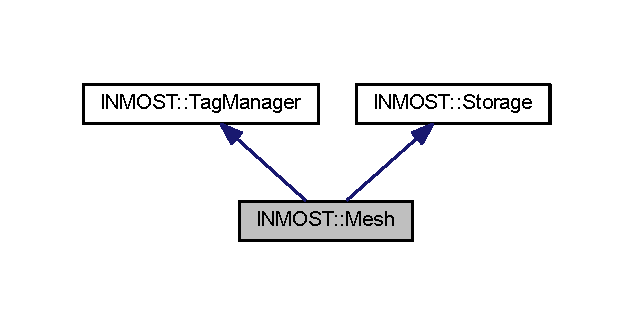
\includegraphics[width=304pt]{classINMOST_1_1Mesh__inherit__graph}
\end{center}
\end{figure}


Collaboration diagram for I\-N\-M\-O\-S\-T\-:\-:Mesh\-:\nopagebreak
\begin{figure}[H]
\begin{center}
\leavevmode
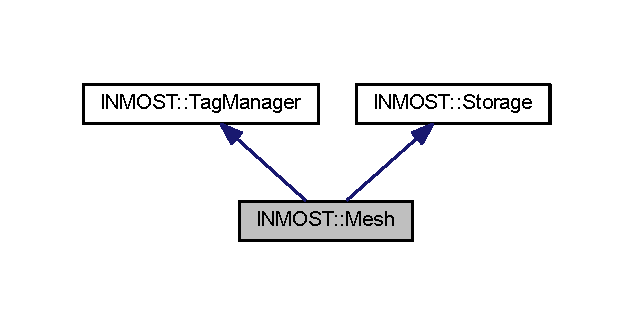
\includegraphics[width=304pt]{classINMOST_1_1Mesh__coll__graph}
\end{center}
\end{figure}
\subsection*{Classes}
\begin{DoxyCompactItemize}
\item 
class \hyperlink{classINMOST_1_1Mesh_1_1base__iterator}{base\-\_\-iterator}
\item 
class \hyperlink{classINMOST_1_1Mesh_1_1BulkComparator}{Bulk\-Comparator}
\item 
class \hyperlink{classINMOST_1_1Mesh_1_1BulkDFComparator}{Bulk\-D\-F\-Comparator}
\item 
class \hyperlink{classINMOST_1_1Mesh_1_1CentroidComparator}{Centroid\-Comparator}
\item 
class \hyperlink{classINMOST_1_1Mesh_1_1exchange__data}{exchange\-\_\-data}
\item 
class \hyperlink{classINMOST_1_1Mesh_1_1GlobalIDComparator}{Global\-I\-D\-Comparator}
\item 
class \hyperlink{classINMOST_1_1Mesh_1_1IerarhyComparator}{Ierarhy\-Comparator}
\item 
class \hyperlink{classINMOST_1_1Mesh_1_1IntegerComparator}{Integer\-Comparator}
\item 
class \hyperlink{classINMOST_1_1Mesh_1_1IntegerDFComparator}{Integer\-D\-F\-Comparator}
\item 
class \hyperlink{classINMOST_1_1Mesh_1_1RealComparator}{Real\-Comparator}
\item 
class \hyperlink{classINMOST_1_1Mesh_1_1RealDFComparator}{Real\-D\-F\-Comparator}
\end{DoxyCompactItemize}
\subsection*{Public Types}
\begin{DoxyCompactItemize}
\item 
enum {\bfseries Mesh\-State} \{ {\bfseries Serial}, 
{\bfseries Parallel}
 \}
\item 
enum {\bfseries Action} \{ {\bfseries A\-Ghost}, 
{\bfseries A\-Migrate}
 \}
\item 
enum {\bfseries Prepare} \{ {\bfseries Unknown\-Size}, 
{\bfseries Unknown\-Source}
 \}
\item 
\hypertarget{classINMOST_1_1Mesh_ae9055f423fc6502c7e476ce1247904e6}{typedef chunk\-\_\-array$<$ \hyperlink{classINMOST_1_1Storage_aec96942bc647417a801e2895b45964d2}{integer}, \\*
chunk\-\_\-bits\-\_\-empty $>$ {\bfseries empty\-\_\-container}}\label{classINMOST_1_1Mesh_ae9055f423fc6502c7e476ce1247904e6}

\item 
\hypertarget{classINMOST_1_1Mesh_a7a8e9f6b0b8eea367c332c36320d4c02}{typedef chunk\-\_\-array$<$ \hyperlink{classINMOST_1_1Storage_aec96942bc647417a801e2895b45964d2}{integer}, \\*
chunk\-\_\-bits\-\_\-elems $>$ {\bfseries links\-\_\-container}}\label{classINMOST_1_1Mesh_a7a8e9f6b0b8eea367c332c36320d4c02}

\item 
\hypertarget{classINMOST_1_1Mesh_a7aa5359ad0ee39a9a35ed7230d8bd3e1}{typedef Tag\-Manager\-::sparse\-\_\-sub\-\_\-type {\bfseries sparse\-\_\-type}}\label{classINMOST_1_1Mesh_a7aa5359ad0ee39a9a35ed7230d8bd3e1}

\item 
\hypertarget{classINMOST_1_1Mesh_a108a6bf9c3b9ce9d446c891a23329ef1}{typedef \\*
\hyperlink{structINMOST_1_1TagManager_1_1sparse__sub__record}{Tag\-Manager\-::sparse\-\_\-sub\-\_\-record} {\bfseries sparse\-\_\-rec}}\label{classINMOST_1_1Mesh_a108a6bf9c3b9ce9d446c891a23329ef1}

\item 
\hypertarget{classINMOST_1_1Mesh_aa32a7de3dbfafd84c6635212b20aecb7}{typedef sparse\-\_\-type\-::size\-\_\-type {\bfseries senum}}\label{classINMOST_1_1Mesh_aa32a7de3dbfafd84c6635212b20aecb7}

\item 
\hypertarget{classINMOST_1_1Mesh_a06b71cc969ef0d9f4e87e51febbfec3b}{typedef void($\ast$ {\bfseries Reduce\-Operation} )(const \hyperlink{classINMOST_1_1Tag}{Tag} \&tag, const \hyperlink{classINMOST_1_1Element}{Element} \&element, const I\-N\-M\-O\-S\-T\-\_\-\-D\-A\-T\-A\-\_\-\-B\-U\-L\-K\-\_\-\-T\-Y\-P\-E $\ast$recv\-\_\-data, I\-N\-M\-O\-S\-T\-\_\-\-D\-A\-T\-A\-\_\-\-E\-N\-U\-M\-\_\-\-T\-Y\-P\-E recv\-\_\-size)}\label{classINMOST_1_1Mesh_a06b71cc969ef0d9f4e87e51febbfec3b}

\item 
\hypertarget{classINMOST_1_1Mesh_a10e96c6c49203571ef3f391a5e65f5de}{typedef std\-::vector$<$ \hyperlink{classINMOST_1_1Tag}{Tag} $>$ {\bfseries tag\-\_\-set}}\label{classINMOST_1_1Mesh_a10e96c6c49203571ef3f391a5e65f5de}

\item 
\hypertarget{classINMOST_1_1Mesh_a2d97c93d9d3a7bee03180d5cd4372696}{typedef std\-::vector$<$ Handle\-Type $>$ {\bfseries element\-\_\-set}}\label{classINMOST_1_1Mesh_a2d97c93d9d3a7bee03180d5cd4372696}

\item 
\hypertarget{classINMOST_1_1Mesh_a956b5292142d9a206f47a00d3f55b22f}{typedef std\-::vector\\*
$<$ I\-N\-M\-O\-S\-T\-\_\-\-D\-A\-T\-A\-\_\-\-B\-U\-L\-K\-\_\-\-T\-Y\-P\-E $>$ {\bfseries buffer\-\_\-type}}\label{classINMOST_1_1Mesh_a956b5292142d9a206f47a00d3f55b22f}

\item 
\hypertarget{classINMOST_1_1Mesh_ac6ae9912a7097744db789754a90118d5}{typedef std\-::map$<$ int, \\*
element\-\_\-set $>$ {\bfseries proc\-\_\-elements}}\label{classINMOST_1_1Mesh_ac6ae9912a7097744db789754a90118d5}

\item 
\hypertarget{classINMOST_1_1Mesh_ad396ce459946a34ebd8cc5e564ff7e20}{typedef std\-::pair$<$ int, \\*
buffer\-\_\-type $>$ {\bfseries proc\-\_\-buffer\-\_\-type}}\label{classINMOST_1_1Mesh_ad396ce459946a34ebd8cc5e564ff7e20}

\item 
\hypertarget{classINMOST_1_1Mesh_a9cdffb8a47775004fd0b7497d321405c}{typedef std\-::vector\\*
$<$ proc\-\_\-buffer\-\_\-type $>$ {\bfseries exch\-\_\-buffer\-\_\-type}}\label{classINMOST_1_1Mesh_a9cdffb8a47775004fd0b7497d321405c}

\item 
\hypertarget{classINMOST_1_1Mesh_a4d3a085d38c3b8b12d708afef270bca9}{typedef \hyperlink{classINMOST_1_1Mesh_1_1base__iterator}{base\-\_\-iterator}$<$ \hyperlink{classINMOST_1_1Storage}{Storage} $>$ {\bfseries iterator\-Storage}}\label{classINMOST_1_1Mesh_a4d3a085d38c3b8b12d708afef270bca9}

\item 
\hypertarget{classINMOST_1_1Mesh_a37f367f5aa2b0d86940e52a8a93b17e0}{typedef \hyperlink{classINMOST_1_1Mesh_1_1base__iterator}{base\-\_\-iterator}$<$ \hyperlink{classINMOST_1_1Element}{Element} $>$ {\bfseries iterator\-Element}}\label{classINMOST_1_1Mesh_a37f367f5aa2b0d86940e52a8a93b17e0}

\item 
\hypertarget{classINMOST_1_1Mesh_a29a8ae93bb4bbfb4d9ca36b2f324ca00}{typedef \hyperlink{classINMOST_1_1Mesh_1_1base__iterator}{base\-\_\-iterator}$<$ \hyperlink{classINMOST_1_1ElementSet}{Element\-Set} $>$ {\bfseries iterator\-Set}}\label{classINMOST_1_1Mesh_a29a8ae93bb4bbfb4d9ca36b2f324ca00}

\item 
\hypertarget{classINMOST_1_1Mesh_a808ade85adce097c826e100527391b1d}{typedef \hyperlink{classINMOST_1_1Mesh_1_1base__iterator}{base\-\_\-iterator}$<$ \hyperlink{classINMOST_1_1Cell}{Cell} $>$ {\bfseries iterator\-Cell}}\label{classINMOST_1_1Mesh_a808ade85adce097c826e100527391b1d}

\item 
\hypertarget{classINMOST_1_1Mesh_a72b0ec48bb09310671f2cb9fed44d8d4}{typedef \hyperlink{classINMOST_1_1Mesh_1_1base__iterator}{base\-\_\-iterator}$<$ \hyperlink{classINMOST_1_1Face}{Face} $>$ {\bfseries iterator\-Face}}\label{classINMOST_1_1Mesh_a72b0ec48bb09310671f2cb9fed44d8d4}

\item 
\hypertarget{classINMOST_1_1Mesh_ae3c66b43ab828c819ec65f660c93937f}{typedef \hyperlink{classINMOST_1_1Mesh_1_1base__iterator}{base\-\_\-iterator}$<$ \hyperlink{classINMOST_1_1Edge}{Edge} $>$ {\bfseries iterator\-Edge}}\label{classINMOST_1_1Mesh_ae3c66b43ab828c819ec65f660c93937f}

\item 
\hypertarget{classINMOST_1_1Mesh_a972f183065ada503d896cd70d73e95b2}{typedef \hyperlink{classINMOST_1_1Mesh_1_1base__iterator}{base\-\_\-iterator}$<$ \hyperlink{classINMOST_1_1Node}{Node} $>$ {\bfseries iterator\-Node}}\label{classINMOST_1_1Mesh_a972f183065ada503d896cd70d73e95b2}

\item 
\hypertarget{classINMOST_1_1Mesh_ab78adb312fbe274f7a7296f86398514d}{typedef tiny\-\_\-map\\*
$<$ Geometric\-Data, Element\-Type, 5 $>$ {\bfseries Geom\-Param}}\label{classINMOST_1_1Mesh_ab78adb312fbe274f7a7296f86398514d}

\end{DoxyCompactItemize}
\subsection*{Public Member Functions}
\begin{DoxyCompactItemize}
\item 
\hypertarget{classINMOST_1_1Mesh_a99d2f7410acff5bc75b0184890d7decd}{\hyperlink{classINMOST_1_1Storage_aec96942bc647417a801e2895b45964d2}{integer} \hyperlink{classINMOST_1_1Mesh_a99d2f7410acff5bc75b0184890d7decd}{Handle\-Data\-Pos} (Handle\-Type h)}\label{classINMOST_1_1Mesh_a99d2f7410acff5bc75b0184890d7decd}

\begin{DoxyCompactList}\small\item\em For debug purposes. \end{DoxyCompactList}\item 
\hypertarget{classINMOST_1_1Mesh_ab2d7cbbd5950153b3c16e26f1bd50c3d}{\hyperlink{classINMOST_1_1Storage_ae333dfced6fa9cfde0c8e7dcf1b0cc2b}{enumerator} \hyperlink{classINMOST_1_1Mesh_ab2d7cbbd5950153b3c16e26f1bd50c3d}{Memory\-Usage} (Handle\-Type h)}\label{classINMOST_1_1Mesh_ab2d7cbbd5950153b3c16e26f1bd50c3d}

\begin{DoxyCompactList}\small\item\em For parmetis return total number in bytes of occupied memory by element and its data. \end{DoxyCompactList}\item 
\hypertarget{classINMOST_1_1Mesh_aef026100f4ec3b0165a5816558faadc2}{{\bfseries Mesh} (const \hyperlink{classINMOST_1_1Mesh}{Mesh} \&other)}\label{classINMOST_1_1Mesh_aef026100f4ec3b0165a5816558faadc2}

\item 
\hypertarget{classINMOST_1_1Mesh_a83cc916a08f462721b5986abf71005ea}{\hyperlink{classINMOST_1_1Mesh}{Mesh} \& {\bfseries operator=} (\hyperlink{classINMOST_1_1Mesh}{Mesh} const \&other)}\label{classINMOST_1_1Mesh_a83cc916a08f462721b5986abf71005ea}

\item 
Marker\-Type \hyperlink{classINMOST_1_1Mesh_a3d860dda768f1d8b7a1b5cd2066cb504}{Create\-Marker} ()
\begin{DoxyCompactList}\small\item\em Allocate new marker. \end{DoxyCompactList}\item 
void \hyperlink{classINMOST_1_1Mesh_a0872520e92d5fefcb827b239d23e4229}{Release\-Marker} (Marker\-Type n)
\begin{DoxyCompactList}\small\item\em Release marker back for reuse. \end{DoxyCompactList}\item 
\-\_\-\-\_\-\-I\-N\-L\-I\-N\-E void \hyperlink{classINMOST_1_1Mesh_a8ef41098a12fe80cac6f45ee94ef892b}{Set\-Epsilon} (\hyperlink{classINMOST_1_1Storage_a853346784b4a5822a7fac54d8f10f805}{real} e)
\begin{DoxyCompactList}\small\item\em Set tolerance for coordinates comparison. \end{DoxyCompactList}\item 
\-\_\-\-\_\-\-I\-N\-L\-I\-N\-E \hyperlink{classINMOST_1_1Storage_a853346784b4a5822a7fac54d8f10f805}{real} \hyperlink{classINMOST_1_1Mesh_a3651c7afd0489bd19eb83554b63d3a31}{Get\-Epsilon} () const 
\begin{DoxyCompactList}\small\item\em Retrieve tolerance for coordinates comparison. \end{DoxyCompactList}\item 
void \hyperlink{classINMOST_1_1Mesh_a04a2c4cb85d29a3f8bae803b013a52c9}{Set\-Dimensions} (\hyperlink{classINMOST_1_1Storage_aec96942bc647417a801e2895b45964d2}{integer} dim)
\begin{DoxyCompactList}\small\item\em Set number of dimensions for mesh. \end{DoxyCompactList}\item 
\-\_\-\-\_\-\-I\-N\-L\-I\-N\-E \hyperlink{classINMOST_1_1Storage_aec96942bc647417a801e2895b45964d2}{integer} \hyperlink{classINMOST_1_1Mesh_ae7b7567174f1da1fe8317eb8bb1fdc6c}{Get\-Dimensions} () const 
\begin{DoxyCompactList}\small\item\em Get number of dimensions of mesh. \end{DoxyCompactList}\item 
\-\_\-\-\_\-\-I\-N\-L\-I\-N\-E Mesh\-State \hyperlink{classINMOST_1_1Mesh_a8f707f8ed964b9ff6e143a625e193823}{Get\-Mesh\-State} () const 
\begin{DoxyCompactList}\small\item\em Get parallel state of the mesh. \end{DoxyCompactList}\item 
\hypertarget{classINMOST_1_1Mesh_a6b425c08bb3751726402817023c52aef}{\-\_\-\-\_\-\-I\-N\-L\-I\-N\-E const \hyperlink{classINMOST_1_1Tag}{Tag} \& {\bfseries Global\-I\-D\-Tag} () const }\label{classINMOST_1_1Mesh_a6b425c08bb3751726402817023c52aef}

\item 
\hypertarget{classINMOST_1_1Mesh_aa36bf499bff23152a29d2b8bb579c2c3}{\-\_\-\-\_\-\-I\-N\-L\-I\-N\-E const \hyperlink{classINMOST_1_1Tag}{Tag} \& {\bfseries Coords\-Tag} () const }\label{classINMOST_1_1Mesh_aa36bf499bff23152a29d2b8bb579c2c3}

\item 
\hypertarget{classINMOST_1_1Mesh_a31c5dd3ca51b3fa7163755edf1f3b5e8}{\-\_\-\-\_\-\-I\-N\-L\-I\-N\-E const \hyperlink{classINMOST_1_1Tag}{Tag} \& {\bfseries Low\-Conn\-Tag} () const }\label{classINMOST_1_1Mesh_a31c5dd3ca51b3fa7163755edf1f3b5e8}

\item 
\hypertarget{classINMOST_1_1Mesh_a722a9739ed3e0b585dfc814f09a2eaa9}{\-\_\-\-\_\-\-I\-N\-L\-I\-N\-E const \hyperlink{classINMOST_1_1Tag}{Tag} \& {\bfseries High\-Conn\-Tag} () const }\label{classINMOST_1_1Mesh_a722a9739ed3e0b585dfc814f09a2eaa9}

\item 
\hypertarget{classINMOST_1_1Mesh_ad7d9049c7e0f028e334d3fac70acdc6c}{\-\_\-\-\_\-\-I\-N\-L\-I\-N\-E const \hyperlink{classINMOST_1_1Tag}{Tag} \& {\bfseries Markers\-Tag} () const }\label{classINMOST_1_1Mesh_ad7d9049c7e0f028e334d3fac70acdc6c}

\item 
\hypertarget{classINMOST_1_1Mesh_a2b33932803424957939cc2d245ba6f6f}{\-\_\-\-\_\-\-I\-N\-L\-I\-N\-E const \hyperlink{classINMOST_1_1Tag}{Tag} \& {\bfseries Geom\-Type\-Tag} () const }\label{classINMOST_1_1Mesh_a2b33932803424957939cc2d245ba6f6f}

\item 
\hypertarget{classINMOST_1_1Mesh_a1f849b01ef5ebe06d7ef6bb425445bf9}{\-\_\-\-\_\-\-I\-N\-L\-I\-N\-E const \hyperlink{classINMOST_1_1Tag}{Tag} \& {\bfseries Sendto\-Tag} () const }\label{classINMOST_1_1Mesh_a1f849b01ef5ebe06d7ef6bb425445bf9}

\item 
\hypertarget{classINMOST_1_1Mesh_a12f64ee311bb980ea6ec98a62d8c107c}{\-\_\-\-\_\-\-I\-N\-L\-I\-N\-E const \hyperlink{classINMOST_1_1Tag}{Tag} \& {\bfseries Shared\-Tag} () const }\label{classINMOST_1_1Mesh_a12f64ee311bb980ea6ec98a62d8c107c}

\item 
\hypertarget{classINMOST_1_1Mesh_a8dc73de1636fffc74052b7b8c94cfcb6}{\-\_\-\-\_\-\-I\-N\-L\-I\-N\-E const \hyperlink{classINMOST_1_1Tag}{Tag} \& {\bfseries Owner\-Tag} () const }\label{classINMOST_1_1Mesh_a8dc73de1636fffc74052b7b8c94cfcb6}

\item 
\hypertarget{classINMOST_1_1Mesh_a1d3f6d16015c510467e6b2fc53cbc25f}{\-\_\-\-\_\-\-I\-N\-L\-I\-N\-E const \hyperlink{classINMOST_1_1Tag}{Tag} \& {\bfseries Layers\-Tag} () const }\label{classINMOST_1_1Mesh_a1d3f6d16015c510467e6b2fc53cbc25f}

\item 
\hypertarget{classINMOST_1_1Mesh_aca9c676f8de7d824126800aac9728e54}{\-\_\-\-\_\-\-I\-N\-L\-I\-N\-E const \hyperlink{classINMOST_1_1Tag}{Tag} \& {\bfseries Bridge\-Tag} () const }\label{classINMOST_1_1Mesh_aca9c676f8de7d824126800aac9728e54}

\item 
\hypertarget{classINMOST_1_1Mesh_a1f9cef94caadde4eb8ea34c73dbab03a}{\-\_\-\-\_\-\-I\-N\-L\-I\-N\-E const \hyperlink{classINMOST_1_1Tag}{Tag} \& {\bfseries Processors\-Tag} () const }\label{classINMOST_1_1Mesh_a1f9cef94caadde4eb8ea34c73dbab03a}

\item 
\hypertarget{classINMOST_1_1Mesh_ae6ed5e05176a8fc0478a5c515c72aa8a}{\-\_\-\-\_\-\-I\-N\-L\-I\-N\-E const \hyperlink{classINMOST_1_1Tag}{Tag} \& {\bfseries Set\-Name\-Tag} () const }\label{classINMOST_1_1Mesh_ae6ed5e05176a8fc0478a5c515c72aa8a}

\item 
\hypertarget{classINMOST_1_1Mesh_a5b52915cd79134141685f994f5364767}{\-\_\-\-\_\-\-I\-N\-L\-I\-N\-E const \hyperlink{classINMOST_1_1Tag}{Tag} \& {\bfseries Set\-Comparator\-Tag} () const }\label{classINMOST_1_1Mesh_a5b52915cd79134141685f994f5364767}

\item 
\-\_\-\-\_\-\-I\-N\-L\-I\-N\-E \hyperlink{classINMOST_1_1Tag}{Tag} \hyperlink{classINMOST_1_1Mesh_a1cd4e1b35b122a5cfc24d6d74229b81b}{Redistribute\-Tag} ()
\begin{DoxyCompactList}\small\item\em Don't put this shortcut to any function directly, as it creates tag inside assign to other object of type \hyperlink{classINMOST_1_1Tag}{Tag} and put this object to functions. \end{DoxyCompactList}\item 
\hyperlink{classINMOST_1_1Tag}{Tag} \hyperlink{classINMOST_1_1Mesh_a02d7bfbdaa069199d3f8b3c3e9e7f151}{Create\-Tag} (std\-::string name, Data\-Type dtype, Element\-Type etype, Element\-Type sparse, I\-N\-M\-O\-S\-T\-\_\-\-D\-A\-T\-A\-\_\-\-E\-N\-U\-M\-\_\-\-T\-Y\-P\-E size=E\-N\-U\-M\-U\-N\-D\-E\-F)
\begin{DoxyCompactList}\small\item\em Create the tag by name, type and size. \end{DoxyCompactList}\item 
\hyperlink{classINMOST_1_1Tag}{Tag} \hyperlink{classINMOST_1_1Mesh_ae43e132d6fd14903e263f00fbcffec51}{Delete\-Tag} (\hyperlink{classINMOST_1_1Tag}{Tag} tag, Element\-Type mask=N\-O\-D\-E$|$E\-D\-G\-E$|$F\-A\-C\-E$|$C\-E\-L\-L$|$E\-S\-E\-T$|$M\-E\-S\-H)
\begin{DoxyCompactList}\small\item\em Remove the data that is represented by the tag from elements of selected type. \end{DoxyCompactList}\item 
\-\_\-\-\_\-\-I\-N\-L\-I\-N\-E iterator\-Tag \hyperlink{classINMOST_1_1Mesh_a2922f80c6c522500a887fe115cf5271d}{Begin\-Tag} ()
\begin{DoxyCompactList}\small\item\em Returns the first tag defined on the mesh. \end{DoxyCompactList}\item 
\-\_\-\-\_\-\-I\-N\-L\-I\-N\-E \hyperlink{classINMOST_1_1Storage_ae333dfced6fa9cfde0c8e7dcf1b0cc2b}{enumerator} \hyperlink{classINMOST_1_1Mesh_a05939bf3f29697b1ffb2005a617ee585}{Number\-Of\-Tags} () const 
\begin{DoxyCompactList}\small\item\em Retrieve the total number of valid tags. \end{DoxyCompactList}\item 
\-\_\-\-\_\-\-I\-N\-L\-I\-N\-E iterator\-Tag \hyperlink{classINMOST_1_1Mesh_ae69466c97ab50182ba143df2a76d5d9f}{End\-Tag} ()
\begin{DoxyCompactList}\small\item\em Returns the indicator for loop to end iteration over tags. \end{DoxyCompactList}\item 
\hyperlink{classINMOST_1_1Node}{Node} \hyperlink{classINMOST_1_1Mesh_a2edad518a07d8d9cfadf7803553a4991}{Create\-Node} (const \hyperlink{classINMOST_1_1Storage_a853346784b4a5822a7fac54d8f10f805}{real} $\ast$coords)
\begin{DoxyCompactList}\small\item\em Create node by given coordinates. \end{DoxyCompactList}\item 
\hypertarget{classINMOST_1_1Mesh_ae3b50ae7b0deede13ab3425cd6547943}{std\-::pair$<$ \hyperlink{classINMOST_1_1Edge}{Edge}, bool $>$ {\bfseries Create\-Edge} (const \hyperlink{classINMOST_1_1ElementArray}{Element\-Array}$<$ \hyperlink{classINMOST_1_1Node}{Node} $>$ \&nodes)}\label{classINMOST_1_1Mesh_ae3b50ae7b0deede13ab3425cd6547943}

\item 
\hypertarget{classINMOST_1_1Mesh_a709a5702c9f1dca9247ddf3efc23f411}{std\-::pair$<$ \hyperlink{classINMOST_1_1Face}{Face}, bool $>$ {\bfseries Create\-Face} (const \hyperlink{classINMOST_1_1ElementArray}{Element\-Array}$<$ \hyperlink{classINMOST_1_1Edge}{Edge} $>$ \&edges)}\label{classINMOST_1_1Mesh_a709a5702c9f1dca9247ddf3efc23f411}

\item 
\hypertarget{classINMOST_1_1Mesh_ae71e8a84e80ee682db190ee94302d8eb}{std\-::pair$<$ \hyperlink{classINMOST_1_1Face}{Face}, bool $>$ {\bfseries Create\-Face} (const \hyperlink{classINMOST_1_1ElementArray}{Element\-Array}$<$ \hyperlink{classINMOST_1_1Node}{Node} $>$ \&nodes)}\label{classINMOST_1_1Mesh_ae71e8a84e80ee682db190ee94302d8eb}

\item 
\hypertarget{classINMOST_1_1Mesh_a66260da2a0bf10c3d4876dea49dfbd58}{std\-::pair$<$ \hyperlink{classINMOST_1_1Cell}{Cell}, bool $>$ {\bfseries Create\-Cell} (const \hyperlink{classINMOST_1_1ElementArray}{Element\-Array}$<$ \hyperlink{classINMOST_1_1Face}{Face} $>$ \&faces, const \hyperlink{classINMOST_1_1ElementArray}{Element\-Array}$<$ \hyperlink{classINMOST_1_1Node}{Node} $>$ \&suggest\-\_\-nodes\-\_\-order=\hyperlink{classINMOST_1_1ElementArray}{Element\-Array}$<$ \hyperlink{classINMOST_1_1Node}{Node} $>$(N\-U\-L\-L))}\label{classINMOST_1_1Mesh_a66260da2a0bf10c3d4876dea49dfbd58}

\item 
\hypertarget{classINMOST_1_1Mesh_a8f493557835c8b2f571cf2af98b1c38f}{std\-::pair$<$ \hyperlink{classINMOST_1_1Cell}{Cell}, bool $>$ {\bfseries Create\-Cell} (const \hyperlink{classINMOST_1_1ElementArray}{Element\-Array}$<$ \hyperlink{classINMOST_1_1Node}{Node} $>$ \&c\-\_\-f\-\_\-nodes, const \hyperlink{classINMOST_1_1Storage_aec96942bc647417a801e2895b45964d2}{integer} $\ast$c\-\_\-f\-\_\-numnodes, \hyperlink{classINMOST_1_1Storage_aec96942bc647417a801e2895b45964d2}{integer} num\-\_\-c\-\_\-faces, const \hyperlink{classINMOST_1_1ElementArray}{Element\-Array}$<$ \hyperlink{classINMOST_1_1Node}{Node} $>$ \&suggest\-\_\-nodes\-\_\-order=\hyperlink{classINMOST_1_1ElementArray}{Element\-Array}$<$ \hyperlink{classINMOST_1_1Node}{Node} $>$(N\-U\-L\-L))}\label{classINMOST_1_1Mesh_a8f493557835c8b2f571cf2af98b1c38f}

\item 
\hypertarget{classINMOST_1_1Mesh_a5a0ca2ce40dfebddd57f006643477234}{std\-::pair$<$ \hyperlink{classINMOST_1_1Cell}{Cell}, bool $>$ {\bfseries Create\-Cell} (const \hyperlink{classINMOST_1_1ElementArray}{Element\-Array}$<$ \hyperlink{classINMOST_1_1Node}{Node} $>$ \&c\-\_\-nodes, const \hyperlink{classINMOST_1_1Storage_aec96942bc647417a801e2895b45964d2}{integer} $\ast$c\-\_\-f\-\_\-nodeinds, const \hyperlink{classINMOST_1_1Storage_aec96942bc647417a801e2895b45964d2}{integer} $\ast$c\-\_\-f\-\_\-numnodes, \hyperlink{classINMOST_1_1Storage_aec96942bc647417a801e2895b45964d2}{integer} num\-\_\-c\-\_\-faces, const \hyperlink{classINMOST_1_1ElementArray}{Element\-Array}$<$ \hyperlink{classINMOST_1_1Node}{Node} $>$ \&suggest\-\_\-nodes\-\_\-order=\hyperlink{classINMOST_1_1ElementArray}{Element\-Array}$<$ \hyperlink{classINMOST_1_1Node}{Node} $>$(N\-U\-L\-L))}\label{classINMOST_1_1Mesh_a5a0ca2ce40dfebddd57f006643477234}

\item 
\hypertarget{classINMOST_1_1Mesh_a13c27ec28c027eaf82475a35ab97b0ad}{std\-::pair$<$ \hyperlink{classINMOST_1_1ElementSet}{Element\-Set}, bool $>$ {\bfseries Create\-Set} (std\-::string name)}\label{classINMOST_1_1Mesh_a13c27ec28c027eaf82475a35ab97b0ad}

\item 
\hyperlink{classINMOST_1_1ElementSet}{Element\-Set} \hyperlink{classINMOST_1_1Mesh_a5223aa8af17d63c7be40027ff789df7e}{Get\-Set} (std\-::string name)
\begin{DoxyCompactList}\small\item\em Retrieve set by name. \end{DoxyCompactList}\item 
\hypertarget{classINMOST_1_1Mesh_a031ce76512ea59b68cad89aca64b8da7}{\hyperlink{classINMOST_1_1ElementArray}{Element\-Array}$<$ \hyperlink{classINMOST_1_1ElementSet}{Element\-Set} $>$ \hyperlink{classINMOST_1_1Mesh_a031ce76512ea59b68cad89aca64b8da7}{Get\-Sets\-By\-Prefix} (std\-::string prefix)}\label{classINMOST_1_1Mesh_a031ce76512ea59b68cad89aca64b8da7}

\begin{DoxyCompactList}\small\item\em Retrieve all the sets whose names start with given prefix. \end{DoxyCompactList}\item 
\hypertarget{classINMOST_1_1Mesh_a9e00078afcbee494f8e4c02d1e088203}{Handle\-Type {\bfseries Last\-Created} () const }\label{classINMOST_1_1Mesh_a9e00078afcbee494f8e4c02d1e088203}

\item 
\hypertarget{classINMOST_1_1Mesh_ab446c474d012ad8a16e82cf8b297d084}{bool {\bfseries is\-Valid\-Handle\-Range} (Handle\-Type h) const }\label{classINMOST_1_1Mesh_ab446c474d012ad8a16e82cf8b297d084}

\item 
\hypertarget{classINMOST_1_1Mesh_a05701da4bd3ed8ca69bbcca256c2b0e2}{bool {\bfseries is\-Valid\-Element} (\hyperlink{classINMOST_1_1Storage_aec96942bc647417a801e2895b45964d2}{integer} etypenum, \hyperlink{classINMOST_1_1Storage_aec96942bc647417a801e2895b45964d2}{integer} lid) const }\label{classINMOST_1_1Mesh_a05701da4bd3ed8ca69bbcca256c2b0e2}

\item 
\hypertarget{classINMOST_1_1Mesh_aed6fa04f985b48852a2fd6305364983e}{bool {\bfseries is\-Valid\-Element} (Element\-Type etype, \hyperlink{classINMOST_1_1Storage_aec96942bc647417a801e2895b45964d2}{integer} lid) const }\label{classINMOST_1_1Mesh_aed6fa04f985b48852a2fd6305364983e}

\item 
\hypertarget{classINMOST_1_1Mesh_aefe80cb31b7763f7124d013050c21e3e}{bool {\bfseries is\-Valid\-Element} (Handle\-Type h) const }\label{classINMOST_1_1Mesh_aefe80cb31b7763f7124d013050c21e3e}

\item 
Handle\-Type \hyperlink{classINMOST_1_1Mesh_a116f510afe89689b615fa73b29bc6f59}{Find\-Shared\-Adjacency} (const Handle\-Type $\ast$arr, \hyperlink{classINMOST_1_1Storage_ae333dfced6fa9cfde0c8e7dcf1b0cc2b}{enumerator} num) const 
\begin{DoxyCompactList}\small\item\em Retrieve upper adjacent that is shared by multiple lower adjacencies. \end{DoxyCompactList}\item 
\hypertarget{classINMOST_1_1Mesh_ae5191aea52d0cb3b8719500bc98d72df}{void {\bfseries Reorder\-Empty} (Element\-Type reordertypes)}\label{classINMOST_1_1Mesh_ae5191aea52d0cb3b8719500bc98d72df}

\item 
\hypertarget{classINMOST_1_1Mesh_acc1b5232061e8f615d962c55dc5397c6}{void {\bfseries Reorder\-Apply} (\hyperlink{classINMOST_1_1Tag}{Tag} index, Element\-Type mask)}\label{classINMOST_1_1Mesh_acc1b5232061e8f615d962c55dc5397c6}

\item 
\hypertarget{classINMOST_1_1Mesh_a73e1126542b6778477ec51bf61dd35d1}{void {\bfseries Restore\-Cell\-Nodes} (Handle\-Type hc, \hyperlink{classINMOST_1_1ElementArray}{Element\-Array}$<$ \hyperlink{classINMOST_1_1Node}{Node} $>$ \&ret)}\label{classINMOST_1_1Mesh_a73e1126542b6778477ec51bf61dd35d1}

\item 
\hyperlink{classINMOST_1_1Storage_a853346784b4a5822a7fac54d8f10f805}{real} \& \hyperlink{classINMOST_1_1Mesh_afa084c637bc9f6850ed77fbb7778d404}{Real} (Handle\-Type h, const \hyperlink{classINMOST_1_1Tag}{Tag} \&tag)
\begin{DoxyCompactList}\small\item\em Returns a reference to inner memory location of the first element of the array of real values. \end{DoxyCompactList}\item 
\hyperlink{classINMOST_1_1Storage_aec96942bc647417a801e2895b45964d2}{integer} \& \hyperlink{classINMOST_1_1Mesh_aa9d44832b3e826a2b61c8e91c5457fbf}{Integer} (Handle\-Type h, const \hyperlink{classINMOST_1_1Tag}{Tag} \&tag)
\begin{DoxyCompactList}\small\item\em Returns a reference to inner memory location of the first element of the array of integer values. \end{DoxyCompactList}\item 
\hyperlink{classINMOST_1_1Storage_ae429556af77094077d212e0ac23c8cfc}{bulk} \& \hyperlink{classINMOST_1_1Mesh_a9df5a8793e5cd8e38182de107d381d9e}{Bulk} (Handle\-Type h, const \hyperlink{classINMOST_1_1Tag}{Tag} \&tag)
\begin{DoxyCompactList}\small\item\em Returns a reference in inner representation to the first element of array of bytes. \end{DoxyCompactList}\item 
\hyperlink{classINMOST_1_1Storage_a8674802045ec170a3c9d0e3281545b54}{reference} \& \hyperlink{classINMOST_1_1Mesh_acfa8b2f65d63edbbed90d865ab6f5314}{Reference} (Handle\-Type h, const \hyperlink{classINMOST_1_1Tag}{Tag} \&tag)
\begin{DoxyCompactList}\small\item\em Returns a reference in inner representation to the first element of array of element handles. \end{DoxyCompactList}\item 
\hyperlink{classINMOST_1_1Storage_a430e5358d435befb38169beef593527e}{real\-\_\-array} \hyperlink{classINMOST_1_1Mesh_a06bdd4e7c0d26750ca0aa40e03fc7d4c}{Real\-Array} (Handle\-Type h, const \hyperlink{classINMOST_1_1Tag}{Tag} \&tag)
\begin{DoxyCompactList}\small\item\em Returns an array of real values. \end{DoxyCompactList}\item 
\hyperlink{classINMOST_1_1Storage_a4d1637367f0487eb778894b57fc94647}{integer\-\_\-array} \hyperlink{classINMOST_1_1Mesh_ac0bbbfafae1405bd27b726bdbb4c2cdd}{Integer\-Array} (Handle\-Type h, const \hyperlink{classINMOST_1_1Tag}{Tag} \&tag)
\begin{DoxyCompactList}\small\item\em Returns an array of integer values. \end{DoxyCompactList}\item 
\hyperlink{classINMOST_1_1Storage_a6e49b2a38cb55dd59529bd23e8b1b852}{bulk\-\_\-array} \hyperlink{classINMOST_1_1Mesh_ae496bab413c4a6103ee62ae3903e95fe}{Bulk\-Array} (Handle\-Type h, const \hyperlink{classINMOST_1_1Tag}{Tag} \&tag)
\begin{DoxyCompactList}\small\item\em Returns an array of bytes. \end{DoxyCompactList}\item 
\hyperlink{classINMOST_1_1Storage_1_1reference__array}{reference\-\_\-array} \hyperlink{classINMOST_1_1Mesh_ac211da4cbe1dc33394c9b725b64b1e86}{Reference\-Array} (Handle\-Type h, const \hyperlink{classINMOST_1_1Tag}{Tag} \&tag)
\begin{DoxyCompactList}\small\item\em Returns an array of element handles. \end{DoxyCompactList}\item 
\hyperlink{classINMOST_1_1Storage_a853346784b4a5822a7fac54d8f10f805}{real} \& \hyperlink{classINMOST_1_1Mesh_a90e88bbdedcf71c3226f3dc94da66807}{Real\-D\-F} (Handle\-Type h, const \hyperlink{classINMOST_1_1Tag}{Tag} \&tag)
\begin{DoxyCompactList}\small\item\em Returns a reference to inner memory location of the first element of the array of real values. \end{DoxyCompactList}\item 
\hyperlink{classINMOST_1_1Storage_aec96942bc647417a801e2895b45964d2}{integer} \& \hyperlink{classINMOST_1_1Mesh_a3dd3068d4db02871478bea86fce38945}{Integer\-D\-F} (Handle\-Type h, const \hyperlink{classINMOST_1_1Tag}{Tag} \&tag)
\begin{DoxyCompactList}\small\item\em Returns a reference to inner memory location of the first element of the array of integer values. \end{DoxyCompactList}\item 
\hyperlink{classINMOST_1_1Storage_ae429556af77094077d212e0ac23c8cfc}{bulk} \& \hyperlink{classINMOST_1_1Mesh_a88229181252531147051badf5a05e263}{Bulk\-D\-F} (Handle\-Type h, const \hyperlink{classINMOST_1_1Tag}{Tag} \&tag)
\begin{DoxyCompactList}\small\item\em Returns a reference in dense array to the first element of constant size array of bytes. \end{DoxyCompactList}\item 
\hyperlink{classINMOST_1_1Storage_a8674802045ec170a3c9d0e3281545b54}{reference} \& \hyperlink{classINMOST_1_1Mesh_ab5abf1a33ab21a0c60338a97287fc115}{Reference\-D\-F} (Handle\-Type h, const \hyperlink{classINMOST_1_1Tag}{Tag} \&tag)
\begin{DoxyCompactList}\small\item\em Returns a reference in dense array to the first element of constant size array of element handles. \end{DoxyCompactList}\item 
\hyperlink{classINMOST_1_1Storage_a430e5358d435befb38169beef593527e}{real\-\_\-array} \hyperlink{classINMOST_1_1Mesh_a8527fa3c2f6ece108b5abce389566365}{Real\-Array\-D\-F} (Handle\-Type h, const \hyperlink{classINMOST_1_1Tag}{Tag} \&tag)
\begin{DoxyCompactList}\small\item\em Returns an array of real values in dense array. \end{DoxyCompactList}\item 
\hyperlink{classINMOST_1_1Storage_a4d1637367f0487eb778894b57fc94647}{integer\-\_\-array} \hyperlink{classINMOST_1_1Mesh_a9d5351b2b6e7f7824598cb46b3c35118}{Integer\-Array\-D\-F} (Handle\-Type h, const \hyperlink{classINMOST_1_1Tag}{Tag} \&tag)
\begin{DoxyCompactList}\small\item\em Returns an array of integer values in dense array. \end{DoxyCompactList}\item 
\hyperlink{classINMOST_1_1Storage_a6e49b2a38cb55dd59529bd23e8b1b852}{bulk\-\_\-array} \hyperlink{classINMOST_1_1Mesh_a53d63f6a251db48695306180f22ff67e}{Bulk\-Array\-D\-F} (Handle\-Type h, const \hyperlink{classINMOST_1_1Tag}{Tag} \&tag)
\begin{DoxyCompactList}\small\item\em Returns an array of bytes in dense array. \end{DoxyCompactList}\item 
\hyperlink{classINMOST_1_1Storage_1_1reference__array}{reference\-\_\-array} \hyperlink{classINMOST_1_1Mesh_a92ba4c935940111e2c9584a9cc96fe6f}{Reference\-Array\-D\-F} (Handle\-Type h, const \hyperlink{classINMOST_1_1Tag}{Tag} \&tag)
\begin{DoxyCompactList}\small\item\em Returns an array of element handles in dense array. \end{DoxyCompactList}\item 
\hyperlink{classINMOST_1_1Storage_a853346784b4a5822a7fac54d8f10f805}{real} \& \hyperlink{classINMOST_1_1Mesh_a679a4a6ed4e4508126919b8fc8fea27a}{Real\-D\-V} (Handle\-Type h, const \hyperlink{classINMOST_1_1Tag}{Tag} \&tag)
\begin{DoxyCompactList}\small\item\em Returns a reference in dense array to the first element of variable size array of real values. \end{DoxyCompactList}\item 
\hyperlink{classINMOST_1_1Storage_aec96942bc647417a801e2895b45964d2}{integer} \& \hyperlink{classINMOST_1_1Mesh_af20ebec0bab305054c5960d7683bfcfd}{Integer\-D\-V} (Handle\-Type h, const \hyperlink{classINMOST_1_1Tag}{Tag} \&tag)
\begin{DoxyCompactList}\small\item\em Returns a reference in dense array to the first element of variable size array of integer values. \end{DoxyCompactList}\item 
\hyperlink{classINMOST_1_1Storage_ae429556af77094077d212e0ac23c8cfc}{bulk} \& \hyperlink{classINMOST_1_1Mesh_a35a62a1c63ac51297dddabb1312f32d1}{Bulk\-D\-V} (Handle\-Type h, const \hyperlink{classINMOST_1_1Tag}{Tag} \&tag)
\begin{DoxyCompactList}\small\item\em Returns a reference in dense array to the first element of variable size array of bytes. \end{DoxyCompactList}\item 
\hyperlink{classINMOST_1_1Storage_a8674802045ec170a3c9d0e3281545b54}{reference} \& \hyperlink{classINMOST_1_1Mesh_ac87430b220565362949e68b073e07c8a}{Reference\-D\-V} (Handle\-Type h, const \hyperlink{classINMOST_1_1Tag}{Tag} \&tag)
\begin{DoxyCompactList}\small\item\em Returns a reference in dense array to the first element of variable size array of element handles. \end{DoxyCompactList}\item 
\hyperlink{classINMOST_1_1Storage_a430e5358d435befb38169beef593527e}{real\-\_\-array} \hyperlink{classINMOST_1_1Mesh_ae7a5f7d22e5b9f7c01b9741719b853dc}{Real\-Array\-D\-V} (Handle\-Type h, const \hyperlink{classINMOST_1_1Tag}{Tag} \&tag)
\begin{DoxyCompactList}\small\item\em Returns an array of real values in dense array of variable size. \end{DoxyCompactList}\item 
\hyperlink{classINMOST_1_1Storage_a4d1637367f0487eb778894b57fc94647}{integer\-\_\-array} \hyperlink{classINMOST_1_1Mesh_ad74aed700689551567039dfddfbf5971}{Integer\-Array\-D\-V} (Handle\-Type h, const \hyperlink{classINMOST_1_1Tag}{Tag} \&tag)
\begin{DoxyCompactList}\small\item\em Returns an array of integer values in dense array of variable size. \end{DoxyCompactList}\item 
\hyperlink{classINMOST_1_1Storage_a6e49b2a38cb55dd59529bd23e8b1b852}{bulk\-\_\-array} \hyperlink{classINMOST_1_1Mesh_a042974abc70e48b9dc84714ca1a50655}{Bulk\-Array\-D\-V} (Handle\-Type h, const \hyperlink{classINMOST_1_1Tag}{Tag} \&tag)
\begin{DoxyCompactList}\small\item\em Returns an array of bytes in dense array of variable size. \end{DoxyCompactList}\item 
\hyperlink{classINMOST_1_1Storage_1_1reference__array}{reference\-\_\-array} \hyperlink{classINMOST_1_1Mesh_aa2a8c6f6d53a863be14b2c137de4eff5}{Reference\-Array\-D\-V} (Handle\-Type h, const \hyperlink{classINMOST_1_1Tag}{Tag} \&tag)
\begin{DoxyCompactList}\small\item\em Returns an array of element handles in dense array of variable size. \end{DoxyCompactList}\item 
void \hyperlink{classINMOST_1_1Mesh_ab0eb79ff655477197ce21dedae4712d4}{Set\-Marker} (Handle\-Type h, Marker\-Type n)
\begin{DoxyCompactList}\small\item\em Set a marker on the element represented by handle. \end{DoxyCompactList}\item 
void \hyperlink{classINMOST_1_1Mesh_a84ff5329978e77876ca6b1b3ed9b5c39}{Set\-Marker\-Array} (const Handle\-Type $\ast$h, \hyperlink{classINMOST_1_1Storage_ae333dfced6fa9cfde0c8e7dcf1b0cc2b}{enumerator} n, Marker\-Type m)
\begin{DoxyCompactList}\small\item\em Set a marker on the set of handles. \end{DoxyCompactList}\item 
bool \hyperlink{classINMOST_1_1Mesh_a2c8a00522e2b06a0b59e25cae119a237}{Get\-Marker} (Handle\-Type h, Marker\-Type n) const 
\begin{DoxyCompactList}\small\item\em Check whether the marker is set one the element. \end{DoxyCompactList}\item 
void \hyperlink{classINMOST_1_1Mesh_aa758ff129bf79eff3c446946e276006c}{Rem\-Marker} (Handle\-Type h, Marker\-Type n)
\begin{DoxyCompactList}\small\item\em Remove the marker from the element. \end{DoxyCompactList}\item 
void \hyperlink{classINMOST_1_1Mesh_a14f8614996be1f7dd81825a447e9f4e8}{Rem\-Marker\-Array} (const Handle\-Type $\ast$h, \hyperlink{classINMOST_1_1Storage_ae333dfced6fa9cfde0c8e7dcf1b0cc2b}{enumerator} n, Marker\-Type m)
\begin{DoxyCompactList}\small\item\em Remove the marker from the set of handles. \end{DoxyCompactList}\item 
\hypertarget{classINMOST_1_1Mesh_a4b688c3af40eeef80d7d365c56be193f}{void \hyperlink{classINMOST_1_1Mesh_a4b688c3af40eeef80d7d365c56be193f}{Clear\-Marker\-Space} (Handle\-Type h)}\label{classINMOST_1_1Mesh_a4b688c3af40eeef80d7d365c56be193f}

\begin{DoxyCompactList}\small\item\em Remove all the markers from the element. \end{DoxyCompactList}\item 
void \hyperlink{classINMOST_1_1Mesh_ab7db80997803b96df82f83c4e53f64ec}{Get\-Marker\-Space} (Handle\-Type h, \hyperlink{classINMOST_1_1Storage_ae429556af77094077d212e0ac23c8cfc}{bulk} copy\mbox{[}Marker\-Fields\mbox{]}) const 
\begin{DoxyCompactList}\small\item\em Get a copy of the bytes that store markers on the element. \end{DoxyCompactList}\item 
void \hyperlink{classINMOST_1_1Mesh_aadcd74b16a7a86db78d2cf5bb814f5a3}{Set\-Marker\-Space} (Handle\-Type h, \hyperlink{classINMOST_1_1Storage_ae429556af77094077d212e0ac23c8cfc}{bulk} source\mbox{[}Marker\-Fields\mbox{]})
\begin{DoxyCompactList}\small\item\em Overwrite the bytes that store markers on the element. \end{DoxyCompactList}\item 
Element\-::adj\-\_\-type \& \hyperlink{classINMOST_1_1Mesh_a1e7462d775868bb6ef687cef8a5198cb}{High\-Conn} (Handle\-Type h)
\begin{DoxyCompactList}\small\item\em Access directly higher order adjacencies of current element with right of modification. \end{DoxyCompactList}\item 
\hypertarget{classINMOST_1_1Mesh_a6728d9a7247c3a1b566fa127785318f7}{Element\-::adj\-\_\-type const \& \hyperlink{classINMOST_1_1Mesh_a6728d9a7247c3a1b566fa127785318f7}{High\-Conn} (Handle\-Type h) const }\label{classINMOST_1_1Mesh_a6728d9a7247c3a1b566fa127785318f7}

\begin{DoxyCompactList}\small\item\em Access directly higher order adjacencies of current element without right of modification. \end{DoxyCompactList}\item 
Element\-::adj\-\_\-type \& \hyperlink{classINMOST_1_1Mesh_ad20f64a301adf9c3fafe28a8f921a791}{Low\-Conn} (Handle\-Type h)
\begin{DoxyCompactList}\small\item\em Access directly lower order adjacencies of current element with right of modification. \end{DoxyCompactList}\item 
\hypertarget{classINMOST_1_1Mesh_ab7f709414cd7ae4464b0e2af48a8e44e}{Element\-::adj\-\_\-type const \& \hyperlink{classINMOST_1_1Mesh_ab7f709414cd7ae4464b0e2af48a8e44e}{Low\-Conn} (Handle\-Type h) const }\label{classINMOST_1_1Mesh_ab7f709414cd7ae4464b0e2af48a8e44e}

\begin{DoxyCompactList}\small\item\em Access directly lower order adjacencies of current element without right of modification. \end{DoxyCompactList}\item 
I\-N\-M\-O\-S\-T\-\_\-\-D\-A\-T\-A\-\_\-\-E\-N\-U\-M\-\_\-\-T\-Y\-P\-E \hyperlink{classINMOST_1_1Mesh_a4a721e7a76dba9bc87c4f014bff013cc}{Get\-Data\-Size} (Handle\-Type h, const \hyperlink{classINMOST_1_1Tag}{Tag} \&tag) const 
\begin{DoxyCompactList}\small\item\em Return the size of the array. \end{DoxyCompactList}\item 
void \hyperlink{classINMOST_1_1Mesh_a8ade9beb68c97be47897b50ce6e4dcb6}{Set\-Data\-Size} (Handle\-Type h, const \hyperlink{classINMOST_1_1Tag}{Tag} \&tag, \hyperlink{classINMOST_1_1Storage_ae333dfced6fa9cfde0c8e7dcf1b0cc2b}{enumerator} new\-\_\-size)
\begin{DoxyCompactList}\small\item\em Sets the size of the array for data of variable size. \end{DoxyCompactList}\item 
void \hyperlink{classINMOST_1_1Mesh_abd9c22bde076d9828752924f1b6cefb1}{Get\-Data} (Handle\-Type h, const \hyperlink{classINMOST_1_1Tag}{Tag} \&tag, \hyperlink{classINMOST_1_1Storage_ae333dfced6fa9cfde0c8e7dcf1b0cc2b}{enumerator} shift, \hyperlink{classINMOST_1_1Storage_ae333dfced6fa9cfde0c8e7dcf1b0cc2b}{enumerator} size, void $\ast$data) const 
\begin{DoxyCompactList}\small\item\em Copy inner data array of size elements to provided array begining from shift element. \end{DoxyCompactList}\item 
void \hyperlink{classINMOST_1_1Mesh_a2e40d1712147e6dc39113d855882743e}{Set\-Data} (Handle\-Type h, const \hyperlink{classINMOST_1_1Tag}{Tag} \&tag, \hyperlink{classINMOST_1_1Storage_ae333dfced6fa9cfde0c8e7dcf1b0cc2b}{enumerator} shift, \hyperlink{classINMOST_1_1Storage_ae333dfced6fa9cfde0c8e7dcf1b0cc2b}{enumerator} size, const void $\ast$data)
\begin{DoxyCompactList}\small\item\em Copy into inner data array of size elements from provided array begining from shift element. \end{DoxyCompactList}\item 
void \hyperlink{classINMOST_1_1Mesh_afab20c754eef0006e3085dc546e893bb}{Del\-Data} (Handle\-Type h, const \hyperlink{classINMOST_1_1Tag}{Tag} \&tag)
\begin{DoxyCompactList}\small\item\em Remove tag data from given element. \end{DoxyCompactList}\item 
void \hyperlink{classINMOST_1_1Mesh_abac72292a681f80f9f112566e3c04bc5}{Del\-Dense\-Data} (Handle\-Type h, const \hyperlink{classINMOST_1_1Tag}{Tag} \&tag)
\begin{DoxyCompactList}\small\item\em Removes data of variable size, clears to zero data of fixed size. \end{DoxyCompactList}\item 
void \hyperlink{classINMOST_1_1Mesh_a21517e19d638410e9a5bdbaf4cc8fd4c}{Del\-Sparse\-Data} (Handle\-Type h, const \hyperlink{classINMOST_1_1Tag}{Tag} \&tag)
\begin{DoxyCompactList}\small\item\em Removes data of variable size and sparse tag data. \end{DoxyCompactList}\item 
bool \hyperlink{classINMOST_1_1Mesh_a14fe30c96eba52f03de5780503116af1}{Have\-Data} (Handle\-Type h, const \hyperlink{classINMOST_1_1Tag}{Tag} \&tag) const 
\begin{DoxyCompactList}\small\item\em Check whether data is present on given element. \end{DoxyCompactList}\item 
\hypertarget{classINMOST_1_1Mesh_a819feef3c5f1206d8bbc6775becc739e}{Element\-::\-Geometric\-Type {\bfseries Get\-Geometric\-Type} (Handle\-Type h) const }\label{classINMOST_1_1Mesh_a819feef3c5f1206d8bbc6775becc739e}

\item 
\hypertarget{classINMOST_1_1Mesh_a497dd8d40df1e33fd3040056a7922549}{void {\bfseries Set\-Geometric\-Type} (Handle\-Type h, Element\-::\-Geometric\-Type type)}\label{classINMOST_1_1Mesh_a497dd8d40df1e33fd3040056a7922549}

\item 
\hyperlink{classINMOST_1_1Storage_aec96942bc647417a801e2895b45964d2}{integer} \& \hyperlink{classINMOST_1_1Mesh_ab9f84a185381a0096fc358e7e2ff5db7}{Global\-I\-D} (Handle\-Type h)
\begin{DoxyCompactList}\small\item\em Retrieve global id of the element with right of modification (dangerous to modify). \end{DoxyCompactList}\item 
\hyperlink{classINMOST_1_1Storage_aec96942bc647417a801e2895b45964d2}{integer} \hyperlink{classINMOST_1_1Mesh_a1c43e6d9cb856c240f084b2f839c2c8c}{Global\-I\-D} (Handle\-Type h) const 
\begin{DoxyCompactList}\small\item\em Retrieve global id of the element without right of modification. \end{DoxyCompactList}\item 
\hyperlink{classINMOST_1_1Storage_aec96942bc647417a801e2895b45964d2}{integer} \hyperlink{classINMOST_1_1Mesh_a2078f4c2589dc14fe6291416ac21050f}{Data\-Local\-I\-D} (Handle\-Type h) const 
\begin{DoxyCompactList}\small\item\em Retrieve position of the data position of current element. \end{DoxyCompactList}\item 
Element\-::\-Status \hyperlink{classINMOST_1_1Mesh_a94963a0f3f1d80ee0785fb8ebd409339}{Get\-Status} (Handle\-Type h) const 
\begin{DoxyCompactList}\small\item\em Retrieve parallel status of the element. \end{DoxyCompactList}\item 
void \hyperlink{classINMOST_1_1Mesh_a666201ee66a5a0f871d17781055b06ac}{Set\-Status} (Handle\-Type h, Element\-::\-Status s)
\begin{DoxyCompactList}\small\item\em Set parallel status of the element. \end{DoxyCompactList}\item 
void \hyperlink{classINMOST_1_1Mesh_a0e2c090ee95e802c4f486a5d98fc6cb0}{Destroy} (Handle\-Type h)
\begin{DoxyCompactList}\small\item\em Completely destroy element from mesh. \end{DoxyCompactList}\item 
\hypertarget{classINMOST_1_1Mesh_a656d48f7478afdc5240295ad97929dab}{void \hyperlink{classINMOST_1_1Mesh_a656d48f7478afdc5240295ad97929dab}{Destroy} (const \hyperlink{classINMOST_1_1Storage}{Storage} \&e)}\label{classINMOST_1_1Mesh_a656d48f7478afdc5240295ad97929dab}

\begin{DoxyCompactList}\small\item\em Shortcut for typed elements. \end{DoxyCompactList}\item 
bool \hyperlink{classINMOST_1_1Mesh_a2b3eaaadcd233cf11deba24d1fd64ad1}{Hide} (Handle\-Type h)
\begin{DoxyCompactList}\small\item\em Hide element from mesh. \end{DoxyCompactList}\item 
bool \hyperlink{classINMOST_1_1Mesh_a3bfe7b75e432280922bfa7293743115c}{Show} (Handle\-Type h)
\begin{DoxyCompactList}\small\item\em Show element from mesh. \end{DoxyCompactList}\item 
bool \hyperlink{classINMOST_1_1Mesh_a569c516120df121980d0585deadd3634}{Delete} (Handle\-Type h)
\begin{DoxyCompactList}\small\item\em This function will hide element in modification state (between Begin\-Modification and End\-Modification) or call Destroy in non-\/modification state. \end{DoxyCompactList}\item 
bool \hyperlink{classINMOST_1_1Mesh_a632e8966cbebd2e82df1edc7474a5993}{Hidden} (Handle\-Type h) const 
\begin{DoxyCompactList}\small\item\em Check whether element is hidden. \end{DoxyCompactList}\item 
bool \hyperlink{classINMOST_1_1Mesh_aaa34219e9c94a2509c7bae2254ea7a14}{New} (Handle\-Type h) const 
\begin{DoxyCompactList}\small\item\em Check whether element is new. \end{DoxyCompactList}\item 
void \hyperlink{classINMOST_1_1Mesh_a887f25126d7a0fc38e238e5c2b033d58}{Compute\-Geometric\-Type} (Handle\-Type h)
\begin{DoxyCompactList}\small\item\em Recompute geometrical type of current element and set it to element. \end{DoxyCompactList}\item 
\hypertarget{classINMOST_1_1Mesh_a09727abab2781d3fbbcff23ca064777b}{I\-N\-M\-O\-S\-T\-\_\-\-D\-A\-T\-A\-\_\-\-E\-N\-U\-M\-\_\-\-T\-Y\-P\-E \hyperlink{classINMOST_1_1Mesh_a09727abab2781d3fbbcff23ca064777b}{Get\-Array\-Capacity} (\hyperlink{classINMOST_1_1Storage_aec96942bc647417a801e2895b45964d2}{integer} etypenum)}\label{classINMOST_1_1Mesh_a09727abab2781d3fbbcff23ca064777b}

\begin{DoxyCompactList}\small\item\em This function is needed by \hyperlink{classINMOST_1_1TagManager}{Tag\-Manager}, may be made private in future follows definition of chunk\-\_\-array to estimate current occupancy of arrays. \end{DoxyCompactList}\item 
void \hyperlink{classINMOST_1_1Mesh_adc92ee8e1fc34b3f3a41f2a1984ab6f2}{Set\-Parallel\-Strategy} (int strategy)
\begin{DoxyCompactList}\small\item\em Set parallel strategy for inner communications. \end{DoxyCompactList}\item 
int \hyperlink{classINMOST_1_1Mesh_a8543798618f286ce2af5ca2d5a0d7b87}{Get\-Parallel\-Strategy} ()
\begin{DoxyCompactList}\small\item\em Retrieve currently set parallel strategy. \end{DoxyCompactList}\item 
void \hyperlink{classINMOST_1_1Mesh_a2e45b137719114d78119bfe487be259f}{Set\-Parallel\-File\-Strategy} (int strategy)
\begin{DoxyCompactList}\small\item\em This strategy correspond only to internal \char`\"{}.\-pmf\char`\"{} mesh format. \end{DoxyCompactList}\item 
int \hyperlink{classINMOST_1_1Mesh_a7a8d32b876d5299b4da51de0f5f5386a}{Get\-Parallel\-File\-Strategy} ()
\begin{DoxyCompactList}\small\item\em Retrieve currently set parallel strategy for \char`\"{}.\-pmf\char`\"{} files. \end{DoxyCompactList}\item 
\hypertarget{classINMOST_1_1Mesh_a35e810a4aa1bebf48a9911304b3b5bce}{int \hyperlink{classINMOST_1_1Mesh_a35e810a4aa1bebf48a9911304b3b5bce}{Get\-Processor\-Rank} ()}\label{classINMOST_1_1Mesh_a35e810a4aa1bebf48a9911304b3b5bce}

\begin{DoxyCompactList}\small\item\em Get rank of current processor. \end{DoxyCompactList}\item 
\hypertarget{classINMOST_1_1Mesh_a7400218ed56f607396affac271954f37}{int \hyperlink{classINMOST_1_1Mesh_a7400218ed56f607396affac271954f37}{Get\-Processors\-Number} ()}\label{classINMOST_1_1Mesh_a7400218ed56f607396affac271954f37}

\begin{DoxyCompactList}\small\item\em Get number of processors. \end{DoxyCompactList}\item 
\hypertarget{classINMOST_1_1Mesh_ae36b17a701ff34b531ebb81ca9c2a8cc}{I\-N\-M\-O\-S\-T\-\_\-\-M\-P\-I\-\_\-\-Comm \hyperlink{classINMOST_1_1Mesh_ae36b17a701ff34b531ebb81ca9c2a8cc}{Get\-Communicator} ()}\label{classINMOST_1_1Mesh_ae36b17a701ff34b531ebb81ca9c2a8cc}

\begin{DoxyCompactList}\small\item\em Retrieve M\-P\-I communicator. \end{DoxyCompactList}\item 
\hypertarget{classINMOST_1_1Mesh_ab60495d087cbd5c893c5322ba0fa2c69}{void \hyperlink{classINMOST_1_1Mesh_ab60495d087cbd5c893c5322ba0fa2c69}{Set\-Communicator} (I\-N\-M\-O\-S\-T\-\_\-\-M\-P\-I\-\_\-\-Comm \-\_\-comm)}\label{classINMOST_1_1Mesh_ab60495d087cbd5c893c5322ba0fa2c69}

\begin{DoxyCompactList}\small\item\em Set M\-P\-I communicator. \end{DoxyCompactList}\item 
\hypertarget{classINMOST_1_1Mesh_aafe1b9041308f0855c6be0e05973e660}{void {\bfseries Resolve\-Shared} ()}\label{classINMOST_1_1Mesh_aafe1b9041308f0855c6be0e05973e660}

\item 
\hypertarget{classINMOST_1_1Mesh_a904f35aec841e85367f6db64d8ce3cb8}{void \hyperlink{classINMOST_1_1Mesh_a904f35aec841e85367f6db64d8ce3cb8}{Remove\-Ghost} ()}\label{classINMOST_1_1Mesh_a904f35aec841e85367f6db64d8ce3cb8}

\begin{DoxyCompactList}\small\item\em Delete all the ghost cells. \end{DoxyCompactList}\item 
void \hyperlink{classINMOST_1_1Mesh_a5cb95f1e8d6b7987496fc8276c86cf3a}{Remove\-Ghost\-Elements} (const Handle\-Type $\ast$ghost, \hyperlink{classINMOST_1_1Storage_ae333dfced6fa9cfde0c8e7dcf1b0cc2b}{enumerator} num)
\begin{DoxyCompactList}\small\item\em Delete some ghost cells provided in array. \end{DoxyCompactList}\item 
\hypertarget{classINMOST_1_1Mesh_a0ac883e455fe795e9a7db3cc8c99ac26}{{\footnotesize template$<$typename E\-Type $>$ }\\void {\bfseries Remove\-Ghost\-Elements} (const \hyperlink{classINMOST_1_1ElementArray}{Element\-Array}$<$ E\-Type $>$ \&ghost)}\label{classINMOST_1_1Mesh_a0ac883e455fe795e9a7db3cc8c99ac26}

\item 
\hypertarget{classINMOST_1_1Mesh_a5c59c400e41943ea87dbb1f0eff1e2bd}{void {\bfseries Remove\-Ghost\-Elements} (const \hyperlink{classINMOST_1_1ElementSet}{Element\-Set} \&ghost)}\label{classINMOST_1_1Mesh_a5c59c400e41943ea87dbb1f0eff1e2bd}

\item 
void \hyperlink{classINMOST_1_1Mesh_ae39e30b11f35de81d2a9b8451ef87391}{Assign\-Global\-I\-D} (Element\-Type mask)
\begin{DoxyCompactList}\small\item\em Assign unique numbers to elements. \end{DoxyCompactList}\item 
void \hyperlink{classINMOST_1_1Mesh_aa3e1067bc3139bb0216f7ce3c1936734}{Exchange\-Data} (const \hyperlink{classINMOST_1_1Tag}{Tag} \&tag, Element\-Type mask, Marker\-Type select)
\begin{DoxyCompactList}\small\item\em Update data from Shared elements to Ghost elements. \end{DoxyCompactList}\item 
void \hyperlink{classINMOST_1_1Mesh_a35ca81c3d8a01aa6a9ce983769fa03cd}{Exchange\-Data\-Begin} (const \hyperlink{classINMOST_1_1Tag}{Tag} \&tag, Element\-Type mask, Marker\-Type select, \hyperlink{classINMOST_1_1Mesh_1_1exchange__data}{exchange\-\_\-data} \&storage)
\begin{DoxyCompactList}\small\item\em Start asynchronous synchronization of data. \end{DoxyCompactList}\item 
void \hyperlink{classINMOST_1_1Mesh_a443828dada7d0fe8ebcf8040593e1ac1}{Exchange\-Data\-End} (const \hyperlink{classINMOST_1_1Tag}{Tag} \&tag, Element\-Type mask, Marker\-Type select, \hyperlink{classINMOST_1_1Mesh_1_1exchange__data}{exchange\-\_\-data} \&storage)
\begin{DoxyCompactList}\small\item\em Complete asynchronous synchronization of data. \end{DoxyCompactList}\item 
void \hyperlink{classINMOST_1_1Mesh_a064ee931e0f6a75dae38a65d3e8603af}{Exchange\-Data} (const tag\-\_\-set \&tags, Element\-Type mask, Marker\-Type select)
\begin{DoxyCompactList}\small\item\em This function will perform exchange of multiple data tags. \end{DoxyCompactList}\item 
void \hyperlink{classINMOST_1_1Mesh_a418d72493b24344d247b811bd980b3a9}{Exchange\-Data\-Begin} (const tag\-\_\-set \&tags, Element\-Type mask, Marker\-Type select, \hyperlink{classINMOST_1_1Mesh_1_1exchange__data}{exchange\-\_\-data} \&storage)
\begin{DoxyCompactList}\small\item\em This function will initialize exchange of multiple data tags. \end{DoxyCompactList}\item 
void \hyperlink{classINMOST_1_1Mesh_aa49bac8c58e4e610eb4c7ec7dd9f4b96}{Exchange\-Data\-End} (const tag\-\_\-set \&tags, Element\-Type mask, Marker\-Type select, \hyperlink{classINMOST_1_1Mesh_1_1exchange__data}{exchange\-\_\-data} \&storage)
\begin{DoxyCompactList}\small\item\em This function will finalize exchange of multiple data tags. \end{DoxyCompactList}\item 
void \hyperlink{classINMOST_1_1Mesh_a2d488479041917c975b1e662d642c4a5}{Reduce\-Data} (const \hyperlink{classINMOST_1_1Tag}{Tag} \&tag, Element\-Type mask, Marker\-Type select, Reduce\-Operation op)
\begin{DoxyCompactList}\small\item\em Accumulation of data from ghost elements to shared elements. \end{DoxyCompactList}\item 
void \hyperlink{classINMOST_1_1Mesh_a0597bf77b8438dc79bf791912a2b34d2}{Reduce\-Data\-Begin} (const \hyperlink{classINMOST_1_1Tag}{Tag} \&tag, Element\-Type mask, Marker\-Type select, \hyperlink{classINMOST_1_1Mesh_1_1exchange__data}{exchange\-\_\-data} \&storage)
\begin{DoxyCompactList}\small\item\em This function intializes data reduction. \end{DoxyCompactList}\item 
void \hyperlink{classINMOST_1_1Mesh_aa8273226d8ab6e54baba5db22107df37}{Reduce\-Data\-End} (const \hyperlink{classINMOST_1_1Tag}{Tag} \&tag, Element\-Type mask, Marker\-Type select, Reduce\-Operation op, \hyperlink{classINMOST_1_1Mesh_1_1exchange__data}{exchange\-\_\-data} \&storage)
\begin{DoxyCompactList}\small\item\em This function completes data reduction. \end{DoxyCompactList}\item 
void \hyperlink{classINMOST_1_1Mesh_a831a8bab953c4d8aa102e58bac81c25f}{Reduce\-Data} (const tag\-\_\-set \&tags, Element\-Type mask, Marker\-Type select, Reduce\-Operation op)
\begin{DoxyCompactList}\small\item\em This function will perform reduction of multiple data tags. \end{DoxyCompactList}\item 
void \hyperlink{classINMOST_1_1Mesh_a71c5b8a155e89d182f18e26dbe4b8670}{Reduce\-Data\-Begin} (const tag\-\_\-set \&tags, Element\-Type mask, Marker\-Type select, \hyperlink{classINMOST_1_1Mesh_1_1exchange__data}{exchange\-\_\-data} \&storage)
\begin{DoxyCompactList}\small\item\em This function will initialize reduction of multiple data tags. \end{DoxyCompactList}\item 
void \hyperlink{classINMOST_1_1Mesh_aabf4380aa2878e72cf399f97598dcebe}{Reduce\-Data\-End} (const tag\-\_\-set \&tags, Element\-Type mask, Marker\-Type select, Reduce\-Operation op, \hyperlink{classINMOST_1_1Mesh_1_1exchange__data}{exchange\-\_\-data} \&storage)
\begin{DoxyCompactList}\small\item\em This function will finalize exchange of multiple data tags. \end{DoxyCompactList}\item 
void \hyperlink{classINMOST_1_1Mesh_ae44b9cfcb8964acbd710562df331a51a}{Exchange\-Marked} (enum Action action=A\-Ghost)
\begin{DoxyCompactList}\small\item\em This function realizes two algorithms\-: ghosting of elements and migration of elements. \end{DoxyCompactList}\item 
void \hyperlink{classINMOST_1_1Mesh_ad2f72e7c09e74aa9962721646a627650}{Exchange\-Ghost} (\hyperlink{classINMOST_1_1Storage_aec96942bc647417a801e2895b45964d2}{integer} layers, Element\-Type bridge)
\begin{DoxyCompactList}\small\item\em Form several layers of ghosted cells that are adjacent through bridge elements to current cells. \end{DoxyCompactList}\item 
void \hyperlink{classINMOST_1_1Mesh_ade20ec7c8563e82bf8057bc47a3314b7}{Redistribute} ()
\begin{DoxyCompactList}\small\item\em Migrate all the elements to the new owners prescribed in data corresponding to Redistribute\-Tag. \end{DoxyCompactList}\item 
\hyperlink{classINMOST_1_1Storage_aec96942bc647417a801e2895b45964d2}{integer} \hyperlink{classINMOST_1_1Mesh_a9787ba8c75b41b76b89aeeae2e8aefad}{Enumerate} (Element\-Type mask, \hyperlink{classINMOST_1_1Tag}{Tag} num\-\_\-tag, \hyperlink{classINMOST_1_1Storage_aec96942bc647417a801e2895b45964d2}{integer} start=0, bool define\-\_\-sparse=false)
\begin{DoxyCompactList}\small\item\em Enumerate all elements begining with start and put numeration to data associated with num\-\_\-tag for all elements with given type mask. \end{DoxyCompactList}\item 
\hyperlink{classINMOST_1_1Storage_aec96942bc647417a801e2895b45964d2}{integer} \hyperlink{classINMOST_1_1Mesh_a5dc8c51bea6707ccedc76dba47ea0d48}{Enumerate} (const Handle\-Type $\ast$h, \hyperlink{classINMOST_1_1Storage_ae333dfced6fa9cfde0c8e7dcf1b0cc2b}{enumerator} num, const \hyperlink{classINMOST_1_1Tag}{Tag} \&num\-\_\-tag, \hyperlink{classINMOST_1_1Storage_aec96942bc647417a801e2895b45964d2}{integer} start=0, bool define\-\_\-sparse=true)
\begin{DoxyCompactList}\small\item\em Enumerate all elements begining with start and put numeration to data associated with num\-\_\-tag. \end{DoxyCompactList}\item 
{\footnotesize template$<$typename E\-Type $>$ }\\\hyperlink{classINMOST_1_1Storage_aec96942bc647417a801e2895b45964d2}{integer} \hyperlink{classINMOST_1_1Mesh_a92e7888589b79355fa273ad67c8c9bb5}{Enumerate} (const \hyperlink{classINMOST_1_1ElementArray}{Element\-Array}$<$ E\-Type $>$ \&elements, const \hyperlink{classINMOST_1_1Tag}{Tag} \&num\-\_\-tag, \hyperlink{classINMOST_1_1Storage_aec96942bc647417a801e2895b45964d2}{integer} start=0, bool define\-\_\-sparse=true)
\begin{DoxyCompactList}\small\item\em Enumerate all elements begining with start and put numeration to data associated with num\-\_\-tag. \end{DoxyCompactList}\item 
\hyperlink{classINMOST_1_1Storage_aec96942bc647417a801e2895b45964d2}{integer} \hyperlink{classINMOST_1_1Mesh_a0239ff055f17c76ba19ef8a169b14962}{Enumerate\-Set} (const \hyperlink{classINMOST_1_1ElementSet}{Element\-Set} \&set, const \hyperlink{classINMOST_1_1Tag}{Tag} \&num\-\_\-tag, \hyperlink{classINMOST_1_1Storage_aec96942bc647417a801e2895b45964d2}{integer} start=0, bool define\-\_\-sparse=true)
\begin{DoxyCompactList}\small\item\em Enumerate all elements in the set. \end{DoxyCompactList}\item 
\hyperlink{classINMOST_1_1Storage_aec96942bc647417a801e2895b45964d2}{integer} \hyperlink{classINMOST_1_1Mesh_acc118e878e2cce11985e7384f18700fa}{Total\-Number\-Of} (Element\-Type mask)
\begin{DoxyCompactList}\small\item\em Sum of all physical elements, it excludes ghosted copies. \end{DoxyCompactList}\item 
\hyperlink{classINMOST_1_1Storage_a853346784b4a5822a7fac54d8f10f805}{real} \hyperlink{classINMOST_1_1Mesh_ab90d3db6596d5de6f7ddfd7f72af600f}{Integrate} (\hyperlink{classINMOST_1_1Storage_a853346784b4a5822a7fac54d8f10f805}{real} input)
\begin{DoxyCompactList}\small\item\em Integrate real value over all processors. \end{DoxyCompactList}\item 
\hyperlink{classINMOST_1_1Storage_aec96942bc647417a801e2895b45964d2}{integer} \hyperlink{classINMOST_1_1Mesh_a541bea07883f3afa0be27748edb479ff}{Integrate} (\hyperlink{classINMOST_1_1Storage_aec96942bc647417a801e2895b45964d2}{integer} input)
\begin{DoxyCompactList}\small\item\em Integrate integer value over all processors. \end{DoxyCompactList}\item 
\hyperlink{classINMOST_1_1Storage_a853346784b4a5822a7fac54d8f10f805}{real} \hyperlink{classINMOST_1_1Mesh_abb1eacb17ae889557d9d9d32d7b61ed0}{Integrate} (const \hyperlink{classINMOST_1_1Tag}{Tag} \&t, \hyperlink{classINMOST_1_1Storage_ae333dfced6fa9cfde0c8e7dcf1b0cc2b}{enumerator} entry, Element\-Type mask)
\begin{DoxyCompactList}\small\item\em Integrate data corresponding to tag between all processors. \end{DoxyCompactList}\item 
\hyperlink{classINMOST_1_1Storage_aec96942bc647417a801e2895b45964d2}{integer} \hyperlink{classINMOST_1_1Mesh_a8ac1be80eb3f359e6d2834f212131200}{Exclusive\-Sum} (\hyperlink{classINMOST_1_1Storage_aec96942bc647417a801e2895b45964d2}{integer} input)
\begin{DoxyCompactList}\small\item\em Compute sum of integer values for all processors with rank lower then current, excluding current processor. \end{DoxyCompactList}\item 
\hypertarget{classINMOST_1_1Mesh_a2a95b3b375dde1ba544ec0689ce1610f}{\hyperlink{classINMOST_1_1Storage_a853346784b4a5822a7fac54d8f10f805}{real} {\bfseries Aggregate\-Max} (\hyperlink{classINMOST_1_1Storage_a853346784b4a5822a7fac54d8f10f805}{real} input)}\label{classINMOST_1_1Mesh_a2a95b3b375dde1ba544ec0689ce1610f}

\item 
\hypertarget{classINMOST_1_1Mesh_a473a5c93ff000e34b8c07eb1ec9947a1}{\hyperlink{classINMOST_1_1Storage_aec96942bc647417a801e2895b45964d2}{integer} {\bfseries Aggregate\-Max} (\hyperlink{classINMOST_1_1Storage_aec96942bc647417a801e2895b45964d2}{integer} input)}\label{classINMOST_1_1Mesh_a473a5c93ff000e34b8c07eb1ec9947a1}

\item 
void \hyperlink{classINMOST_1_1Mesh_a5691f394480da7e21c5099e313df03e0}{Recompute\-Parallel\-Storage} (Element\-Type mask)
\begin{DoxyCompactList}\small\item\em Regather ghosted and shared element sets for data exchange. \end{DoxyCompactList}\item 
Element\-Type \hyperlink{classINMOST_1_1Mesh_a9c3acf2a90e25699a64e1f7b4125eaf7}{Synchronize\-Element\-Type} (Element\-Type etype)
\begin{DoxyCompactList}\small\item\em Synchronize bitwise mask of element types between processors. \end{DoxyCompactList}\item 
void \hyperlink{classINMOST_1_1Mesh_a8c7a825072f54b260caa0e8da8877647}{Synchronize\-Marker} (Marker\-Type marker, Element\-Type mask, Sync\-Bit\-Op op)
\begin{DoxyCompactList}\small\item\em Syncronize marker on elements between processors using provided operation. \end{DoxyCompactList}\item 
\hypertarget{classINMOST_1_1Mesh_aecf9564fe8f57e292e7c2267fbe588d6}{void {\bfseries Begin\-Sequential\-Code} ()}\label{classINMOST_1_1Mesh_aecf9564fe8f57e292e7c2267fbe588d6}

\item 
\hypertarget{classINMOST_1_1Mesh_aa4f44fe4031bbe9b68ae0764f4b6d43a}{void {\bfseries End\-Sequential\-Code} ()}\label{classINMOST_1_1Mesh_aa4f44fe4031bbe9b68ae0764f4b6d43a}

\item 
\hypertarget{classINMOST_1_1Mesh_aedac2611fffd95b7cd20ed9540c743fa}{\hyperlink{classINMOST_1_1Element}{Element} {\bfseries Element\-By\-Local\-I\-D} (\hyperlink{classINMOST_1_1Storage_aec96942bc647417a801e2895b45964d2}{integer} etypenum, \hyperlink{classINMOST_1_1Storage_aec96942bc647417a801e2895b45964d2}{integer} lid)}\label{classINMOST_1_1Mesh_aedac2611fffd95b7cd20ed9540c743fa}

\item 
\hypertarget{classINMOST_1_1Mesh_aa9d09a55b27ac2f0f500400648ca38ee}{\hyperlink{classINMOST_1_1Element}{Element} {\bfseries Element\-By\-Local\-I\-D} (Element\-Type etype, \hyperlink{classINMOST_1_1Storage_aec96942bc647417a801e2895b45964d2}{integer} lid)}\label{classINMOST_1_1Mesh_aa9d09a55b27ac2f0f500400648ca38ee}

\item 
\hypertarget{classINMOST_1_1Mesh_a2304ca5cb8a374ecc6b0b5f0f900e349}{\hyperlink{classINMOST_1_1Element}{Element} {\bfseries Element\-By\-Handle} (Handle\-Type h)}\label{classINMOST_1_1Mesh_a2304ca5cb8a374ecc6b0b5f0f900e349}

\item 
\hypertarget{classINMOST_1_1Mesh_ad2584a6bb66add033560e495dbfba53f}{Handle\-Type {\bfseries Next\-Handle} (Handle\-Type h) const }\label{classINMOST_1_1Mesh_ad2584a6bb66add033560e495dbfba53f}

\item 
\hypertarget{classINMOST_1_1Mesh_acf6fc997d82528c82499344d358df8d0}{Handle\-Type {\bfseries Prev\-Handle} (Handle\-Type h) const }\label{classINMOST_1_1Mesh_acf6fc997d82528c82499344d358df8d0}

\item 
\hypertarget{classINMOST_1_1Mesh_a85ef45248dfb8b5126ca81a7bcd409f2}{Handle\-Type {\bfseries Next\-Handle} (Handle\-Type h, Element\-Type mask) const }\label{classINMOST_1_1Mesh_a85ef45248dfb8b5126ca81a7bcd409f2}

\item 
\hypertarget{classINMOST_1_1Mesh_a29b510ecffabe4242b3be375b69a4575}{Handle\-Type {\bfseries Prev\-Handle} (Handle\-Type h, Element\-Type mask) const }\label{classINMOST_1_1Mesh_a29b510ecffabe4242b3be375b69a4575}

\item 
\hypertarget{classINMOST_1_1Mesh_a4f26f7a8fbf7bf0a104b79f2433334a2}{Handle\-Type {\bfseries First\-Handle} () const }\label{classINMOST_1_1Mesh_a4f26f7a8fbf7bf0a104b79f2433334a2}

\item 
\hypertarget{classINMOST_1_1Mesh_a863be497f888170153331f74fae93e06}{Handle\-Type {\bfseries Last\-Handle} () const }\label{classINMOST_1_1Mesh_a863be497f888170153331f74fae93e06}

\item 
\hypertarget{classINMOST_1_1Mesh_a9429b9ce591e027f150443891b23e498}{Handle\-Type {\bfseries First\-Handle} (Element\-Type etype) const }\label{classINMOST_1_1Mesh_a9429b9ce591e027f150443891b23e498}

\item 
\hypertarget{classINMOST_1_1Mesh_aa74548f908cf4966d9ce4a3824d0f5b6}{Handle\-Type {\bfseries Last\-Handle} (Element\-Type etype) const }\label{classINMOST_1_1Mesh_aa74548f908cf4966d9ce4a3824d0f5b6}

\item 
\hypertarget{classINMOST_1_1Mesh_a83562665b8922806e475fa75f79a9b69}{\hyperlink{classINMOST_1_1Node}{Node} {\bfseries Node\-By\-Local\-I\-D} (\hyperlink{classINMOST_1_1Storage_aec96942bc647417a801e2895b45964d2}{integer} lid)}\label{classINMOST_1_1Mesh_a83562665b8922806e475fa75f79a9b69}

\item 
\hypertarget{classINMOST_1_1Mesh_a318f86a5b9807fa73d7e1ffe493fb1d0}{\hyperlink{classINMOST_1_1Edge}{Edge} {\bfseries Edge\-By\-Local\-I\-D} (\hyperlink{classINMOST_1_1Storage_aec96942bc647417a801e2895b45964d2}{integer} lid)}\label{classINMOST_1_1Mesh_a318f86a5b9807fa73d7e1ffe493fb1d0}

\item 
\hypertarget{classINMOST_1_1Mesh_aec7e83bc5a26c47443dd5ae701747ccf}{\hyperlink{classINMOST_1_1Face}{Face} {\bfseries Face\-By\-Local\-I\-D} (\hyperlink{classINMOST_1_1Storage_aec96942bc647417a801e2895b45964d2}{integer} lid)}\label{classINMOST_1_1Mesh_aec7e83bc5a26c47443dd5ae701747ccf}

\item 
\hypertarget{classINMOST_1_1Mesh_a0d502f77d8d56014a67e1715f8628c0f}{\hyperlink{classINMOST_1_1Cell}{Cell} {\bfseries Cell\-By\-Local\-I\-D} (\hyperlink{classINMOST_1_1Storage_aec96942bc647417a801e2895b45964d2}{integer} lid)}\label{classINMOST_1_1Mesh_a0d502f77d8d56014a67e1715f8628c0f}

\item 
\hypertarget{classINMOST_1_1Mesh_af2af21e0963cd29ae7f809e6e2939719}{\hyperlink{classINMOST_1_1ElementSet}{Element\-Set} {\bfseries Eset\-By\-Local\-I\-D} (\hyperlink{classINMOST_1_1Storage_aec96942bc647417a801e2895b45964d2}{integer} lid)}\label{classINMOST_1_1Mesh_af2af21e0963cd29ae7f809e6e2939719}

\item 
\hypertarget{classINMOST_1_1Mesh_a5c71407f13fa67febfeb4d0408b9f6f5}{\hyperlink{classINMOST_1_1Storage_aec96942bc647417a801e2895b45964d2}{integer} {\bfseries Node\-Next\-Local\-I\-D} (\hyperlink{classINMOST_1_1Storage_aec96942bc647417a801e2895b45964d2}{integer} lid) const }\label{classINMOST_1_1Mesh_a5c71407f13fa67febfeb4d0408b9f6f5}

\item 
\hypertarget{classINMOST_1_1Mesh_afabec0ed03dc7e55a3f59bc3793bb32f}{\hyperlink{classINMOST_1_1Storage_aec96942bc647417a801e2895b45964d2}{integer} {\bfseries Edge\-Next\-Local\-I\-D} (\hyperlink{classINMOST_1_1Storage_aec96942bc647417a801e2895b45964d2}{integer} lid) const }\label{classINMOST_1_1Mesh_afabec0ed03dc7e55a3f59bc3793bb32f}

\item 
\hypertarget{classINMOST_1_1Mesh_ad878b5d4497a136f8baa22cd74b964d0}{\hyperlink{classINMOST_1_1Storage_aec96942bc647417a801e2895b45964d2}{integer} {\bfseries Face\-Next\-Local\-I\-D} (\hyperlink{classINMOST_1_1Storage_aec96942bc647417a801e2895b45964d2}{integer} lid) const }\label{classINMOST_1_1Mesh_ad878b5d4497a136f8baa22cd74b964d0}

\item 
\hypertarget{classINMOST_1_1Mesh_ae2a5ae49f2730b44b3fbdd31977f5662}{\hyperlink{classINMOST_1_1Storage_aec96942bc647417a801e2895b45964d2}{integer} {\bfseries Cell\-Next\-Local\-I\-D} (\hyperlink{classINMOST_1_1Storage_aec96942bc647417a801e2895b45964d2}{integer} lid) const }\label{classINMOST_1_1Mesh_ae2a5ae49f2730b44b3fbdd31977f5662}

\item 
\hypertarget{classINMOST_1_1Mesh_a8c45204c5d0f96410a537e93ad1b0aa7}{\hyperlink{classINMOST_1_1Storage_aec96942bc647417a801e2895b45964d2}{integer} {\bfseries Eset\-Next\-Local\-I\-D} (\hyperlink{classINMOST_1_1Storage_aec96942bc647417a801e2895b45964d2}{integer} lid) const }\label{classINMOST_1_1Mesh_a8c45204c5d0f96410a537e93ad1b0aa7}

\item 
\hypertarget{classINMOST_1_1Mesh_ad2adb8d94e20e0feba71b971c0529365}{\hyperlink{classINMOST_1_1Storage_aec96942bc647417a801e2895b45964d2}{integer} {\bfseries Node\-Prev\-Local\-I\-D} (\hyperlink{classINMOST_1_1Storage_aec96942bc647417a801e2895b45964d2}{integer} lid) const }\label{classINMOST_1_1Mesh_ad2adb8d94e20e0feba71b971c0529365}

\item 
\hypertarget{classINMOST_1_1Mesh_ac4a1278d5ee72aa47456b4331fcd1f0a}{\hyperlink{classINMOST_1_1Storage_aec96942bc647417a801e2895b45964d2}{integer} {\bfseries Edge\-Prev\-Local\-I\-D} (\hyperlink{classINMOST_1_1Storage_aec96942bc647417a801e2895b45964d2}{integer} lid) const }\label{classINMOST_1_1Mesh_ac4a1278d5ee72aa47456b4331fcd1f0a}

\item 
\hypertarget{classINMOST_1_1Mesh_a99f91d6922148a16342ac99f2ed45ff1}{\hyperlink{classINMOST_1_1Storage_aec96942bc647417a801e2895b45964d2}{integer} {\bfseries Face\-Prev\-Local\-I\-D} (\hyperlink{classINMOST_1_1Storage_aec96942bc647417a801e2895b45964d2}{integer} lid) const }\label{classINMOST_1_1Mesh_a99f91d6922148a16342ac99f2ed45ff1}

\item 
\hypertarget{classINMOST_1_1Mesh_ab1b35ea5d7f1113518ba8a5a169da55e}{\hyperlink{classINMOST_1_1Storage_aec96942bc647417a801e2895b45964d2}{integer} {\bfseries Cell\-Prev\-Local\-I\-D} (\hyperlink{classINMOST_1_1Storage_aec96942bc647417a801e2895b45964d2}{integer} lid) const }\label{classINMOST_1_1Mesh_ab1b35ea5d7f1113518ba8a5a169da55e}

\item 
\hypertarget{classINMOST_1_1Mesh_a38105dd04581e661e800db9cd9da3b18}{\hyperlink{classINMOST_1_1Storage_aec96942bc647417a801e2895b45964d2}{integer} {\bfseries Eset\-Prev\-Local\-I\-D} (\hyperlink{classINMOST_1_1Storage_aec96942bc647417a801e2895b45964d2}{integer} lid) const }\label{classINMOST_1_1Mesh_a38105dd04581e661e800db9cd9da3b18}

\item 
\hypertarget{classINMOST_1_1Mesh_aa80eb9de7883ddfa176e9acefdc019c7}{\-\_\-\-\_\-\-I\-N\-L\-I\-N\-E \hyperlink{classINMOST_1_1Storage_aec96942bc647417a801e2895b45964d2}{integer} {\bfseries Node\-Last\-Local\-I\-D} () const }\label{classINMOST_1_1Mesh_aa80eb9de7883ddfa176e9acefdc019c7}

\item 
\hypertarget{classINMOST_1_1Mesh_abfa49ab28fa20915aaaea68a6a3ec5ac}{\-\_\-\-\_\-\-I\-N\-L\-I\-N\-E \hyperlink{classINMOST_1_1Storage_aec96942bc647417a801e2895b45964d2}{integer} {\bfseries Edge\-Last\-Local\-I\-D} () const }\label{classINMOST_1_1Mesh_abfa49ab28fa20915aaaea68a6a3ec5ac}

\item 
\hypertarget{classINMOST_1_1Mesh_a5bdf8c4d6d2122d3221dd99e20a430ea}{\-\_\-\-\_\-\-I\-N\-L\-I\-N\-E \hyperlink{classINMOST_1_1Storage_aec96942bc647417a801e2895b45964d2}{integer} {\bfseries Face\-Last\-Local\-I\-D} () const }\label{classINMOST_1_1Mesh_a5bdf8c4d6d2122d3221dd99e20a430ea}

\item 
\hypertarget{classINMOST_1_1Mesh_ac46e642c492612e156a9e85a67b2305d}{\-\_\-\-\_\-\-I\-N\-L\-I\-N\-E \hyperlink{classINMOST_1_1Storage_aec96942bc647417a801e2895b45964d2}{integer} {\bfseries Cell\-Last\-Local\-I\-D} () const }\label{classINMOST_1_1Mesh_ac46e642c492612e156a9e85a67b2305d}

\item 
\hypertarget{classINMOST_1_1Mesh_aaf65bc7bb30f0c80ff196914964f7c1a}{\-\_\-\-\_\-\-I\-N\-L\-I\-N\-E \hyperlink{classINMOST_1_1Storage_aec96942bc647417a801e2895b45964d2}{integer} {\bfseries Eset\-Last\-Local\-I\-D} () const }\label{classINMOST_1_1Mesh_aaf65bc7bb30f0c80ff196914964f7c1a}

\item 
\hypertarget{classINMOST_1_1Mesh_a692fbbc2f3ccaf3b8951c20ec0b14a19}{\hyperlink{classINMOST_1_1Storage_aec96942bc647417a801e2895b45964d2}{integer} {\bfseries Next\-Local\-I\-D} (Element\-Type etype, \hyperlink{classINMOST_1_1Storage_aec96942bc647417a801e2895b45964d2}{integer} lid) const }\label{classINMOST_1_1Mesh_a692fbbc2f3ccaf3b8951c20ec0b14a19}

\item 
\hypertarget{classINMOST_1_1Mesh_a751a12b5299610c2ecbfd935fc3efcfe}{\hyperlink{classINMOST_1_1Storage_aec96942bc647417a801e2895b45964d2}{integer} {\bfseries Prev\-Local\-I\-D} (Element\-Type etype, \hyperlink{classINMOST_1_1Storage_aec96942bc647417a801e2895b45964d2}{integer} lid) const }\label{classINMOST_1_1Mesh_a751a12b5299610c2ecbfd935fc3efcfe}

\item 
\hypertarget{classINMOST_1_1Mesh_a9911e8e9d0e92983cd075b16a5afe2bf}{\hyperlink{classINMOST_1_1Storage_aec96942bc647417a801e2895b45964d2}{integer} {\bfseries First\-Local\-I\-D} (Element\-Type etype) const }\label{classINMOST_1_1Mesh_a9911e8e9d0e92983cd075b16a5afe2bf}

\item 
\hypertarget{classINMOST_1_1Mesh_a06a2ff7416bb492e1cdd095ca9c91e85}{\hyperlink{classINMOST_1_1Storage_aec96942bc647417a801e2895b45964d2}{integer} {\bfseries Last\-Local\-I\-D} (\hyperlink{classINMOST_1_1Storage_aec96942bc647417a801e2895b45964d2}{integer} n) const }\label{classINMOST_1_1Mesh_a06a2ff7416bb492e1cdd095ca9c91e85}

\item 
\hypertarget{classINMOST_1_1Mesh_a34c34383e2eefea680d1217af76a381f}{\hyperlink{classINMOST_1_1Storage_aec96942bc647417a801e2895b45964d2}{integer} {\bfseries Last\-Local\-I\-D} (Element\-Type etype) const }\label{classINMOST_1_1Mesh_a34c34383e2eefea680d1217af76a381f}

\item 
\hypertarget{classINMOST_1_1Mesh_abeeaa462c78ce8a82e0e3e87c55e4455}{\-\_\-\-\_\-\-I\-N\-L\-I\-N\-E \hyperlink{classINMOST_1_1Storage_aec96942bc647417a801e2895b45964d2}{integer} {\bfseries Number\-Of\-Sets} () const }\label{classINMOST_1_1Mesh_abeeaa462c78ce8a82e0e3e87c55e4455}

\item 
\hypertarget{classINMOST_1_1Mesh_a245f0558fa7181cf6789db69c4005b33}{\-\_\-\-\_\-\-I\-N\-L\-I\-N\-E \hyperlink{classINMOST_1_1Storage_aec96942bc647417a801e2895b45964d2}{integer} {\bfseries Number\-Of\-Cells} () const }\label{classINMOST_1_1Mesh_a245f0558fa7181cf6789db69c4005b33}

\item 
\hypertarget{classINMOST_1_1Mesh_a67db1a1d141e8d7cb93ca1284777bb08}{\-\_\-\-\_\-\-I\-N\-L\-I\-N\-E \hyperlink{classINMOST_1_1Storage_aec96942bc647417a801e2895b45964d2}{integer} {\bfseries Number\-Of\-Faces} () const }\label{classINMOST_1_1Mesh_a67db1a1d141e8d7cb93ca1284777bb08}

\item 
\hypertarget{classINMOST_1_1Mesh_a404c19f0ddf24cd968de766cf130b371}{\-\_\-\-\_\-\-I\-N\-L\-I\-N\-E \hyperlink{classINMOST_1_1Storage_aec96942bc647417a801e2895b45964d2}{integer} {\bfseries Number\-Of\-Edges} () const }\label{classINMOST_1_1Mesh_a404c19f0ddf24cd968de766cf130b371}

\item 
\hypertarget{classINMOST_1_1Mesh_a4562c5fd5341705ed706b3c4cfda80fe}{\-\_\-\-\_\-\-I\-N\-L\-I\-N\-E \hyperlink{classINMOST_1_1Storage_aec96942bc647417a801e2895b45964d2}{integer} {\bfseries Number\-Of\-Nodes} () const }\label{classINMOST_1_1Mesh_a4562c5fd5341705ed706b3c4cfda80fe}

\item 
\hypertarget{classINMOST_1_1Mesh_a7aee6d7f5b7432dc34bc7319a9e1e8f4}{\-\_\-\-\_\-\-I\-N\-L\-I\-N\-E \hyperlink{classINMOST_1_1Storage_aec96942bc647417a801e2895b45964d2}{integer} {\bfseries Number\-Of\-Elements} () const }\label{classINMOST_1_1Mesh_a7aee6d7f5b7432dc34bc7319a9e1e8f4}

\item 
\hypertarget{classINMOST_1_1Mesh_a8f8e4c3631d8448e738f26cfc99e6871}{\-\_\-\-\_\-\-I\-N\-L\-I\-N\-E \hyperlink{classINMOST_1_1Storage_aec96942bc647417a801e2895b45964d2}{integer} {\bfseries Number\-Of\-All} () const }\label{classINMOST_1_1Mesh_a8f8e4c3631d8448e738f26cfc99e6871}

\item 
\hypertarget{classINMOST_1_1Mesh_a51c44999830564f5abfbc6920dbe4a1b}{\hyperlink{classINMOST_1_1Storage_aec96942bc647417a801e2895b45964d2}{integer} {\bfseries Number\-Of} (Element\-Type t) const }\label{classINMOST_1_1Mesh_a51c44999830564f5abfbc6920dbe4a1b}

\item 
\hypertarget{classINMOST_1_1Mesh_aaee057ff8894f5920556eea758f45a05}{\hyperlink{classINMOST_1_1Mesh_1_1base__iterator}{iterator\-Storage} \hyperlink{classINMOST_1_1Mesh_aaee057ff8894f5920556eea758f45a05}{Begin} (Element\-Type Types)}\label{classINMOST_1_1Mesh_aaee057ff8894f5920556eea758f45a05}

\begin{DoxyCompactList}\small\item\em These iterators skip invalid elements but don't skip modified elements. \end{DoxyCompactList}\item 
\hypertarget{classINMOST_1_1Mesh_ab4075ba5683113b9da966ee8254c9c98}{\hyperlink{classINMOST_1_1Mesh_1_1base__iterator}{iterator\-Storage} {\bfseries End} ()}\label{classINMOST_1_1Mesh_ab4075ba5683113b9da966ee8254c9c98}

\item 
\hypertarget{classINMOST_1_1Mesh_a5885febfabd0c64ca2147f2508c676ae}{\hyperlink{classINMOST_1_1Mesh_1_1base__iterator}{iterator\-Element} {\bfseries Begin\-Element} (Element\-Type Types)}\label{classINMOST_1_1Mesh_a5885febfabd0c64ca2147f2508c676ae}

\item 
\hypertarget{classINMOST_1_1Mesh_a7ceafaeeef67b517d363d19249c9aae7}{\hyperlink{classINMOST_1_1Mesh_1_1base__iterator}{iterator\-Element} {\bfseries End\-Element} ()}\label{classINMOST_1_1Mesh_a7ceafaeeef67b517d363d19249c9aae7}

\item 
\hypertarget{classINMOST_1_1Mesh_aa5e1a950b5a5f7ad600d55226023b7c9}{\hyperlink{classINMOST_1_1Mesh_1_1base__iterator}{iterator\-Set} {\bfseries Begin\-Set} ()}\label{classINMOST_1_1Mesh_aa5e1a950b5a5f7ad600d55226023b7c9}

\item 
\hypertarget{classINMOST_1_1Mesh_a00f6929baaaf379644dddef6c42fef76}{\hyperlink{classINMOST_1_1Mesh_1_1base__iterator}{iterator\-Set} {\bfseries End\-Set} ()}\label{classINMOST_1_1Mesh_a00f6929baaaf379644dddef6c42fef76}

\item 
\hypertarget{classINMOST_1_1Mesh_a0c7a5c1d76ed3816d0167adac44d0a24}{\hyperlink{classINMOST_1_1Mesh_1_1base__iterator}{iterator\-Cell} {\bfseries Begin\-Cell} ()}\label{classINMOST_1_1Mesh_a0c7a5c1d76ed3816d0167adac44d0a24}

\item 
\hypertarget{classINMOST_1_1Mesh_ad00d0cd949a89a3bf9ff0802d5292e82}{\hyperlink{classINMOST_1_1Mesh_1_1base__iterator}{iterator\-Cell} {\bfseries End\-Cell} ()}\label{classINMOST_1_1Mesh_ad00d0cd949a89a3bf9ff0802d5292e82}

\item 
\hypertarget{classINMOST_1_1Mesh_a8b92935c9e005193abf21f24f701fa07}{\hyperlink{classINMOST_1_1Mesh_1_1base__iterator}{iterator\-Face} {\bfseries Begin\-Face} ()}\label{classINMOST_1_1Mesh_a8b92935c9e005193abf21f24f701fa07}

\item 
\hypertarget{classINMOST_1_1Mesh_a5324c63941c77b2fc4654e5c2774b845}{\hyperlink{classINMOST_1_1Mesh_1_1base__iterator}{iterator\-Face} {\bfseries End\-Face} ()}\label{classINMOST_1_1Mesh_a5324c63941c77b2fc4654e5c2774b845}

\item 
\hypertarget{classINMOST_1_1Mesh_a5215f1e7a43a336c68819a92780b89d5}{\hyperlink{classINMOST_1_1Mesh_1_1base__iterator}{iterator\-Edge} {\bfseries Begin\-Edge} ()}\label{classINMOST_1_1Mesh_a5215f1e7a43a336c68819a92780b89d5}

\item 
\hypertarget{classINMOST_1_1Mesh_ac2f40383f4780d877be0291b5d1c4c85}{\hyperlink{classINMOST_1_1Mesh_1_1base__iterator}{iterator\-Edge} {\bfseries End\-Edge} ()}\label{classINMOST_1_1Mesh_ac2f40383f4780d877be0291b5d1c4c85}

\item 
\hypertarget{classINMOST_1_1Mesh_ab832696d5dfd3340153dedb5dc86974d}{\hyperlink{classINMOST_1_1Mesh_1_1base__iterator}{iterator\-Node} {\bfseries Begin\-Node} ()}\label{classINMOST_1_1Mesh_ab832696d5dfd3340153dedb5dc86974d}

\item 
\hypertarget{classINMOST_1_1Mesh_a424e61945ab061054cf896db3831d7ec}{\hyperlink{classINMOST_1_1Mesh_1_1base__iterator}{iterator\-Node} {\bfseries End\-Node} ()}\label{classINMOST_1_1Mesh_a424e61945ab061054cf896db3831d7ec}

\item 
void \hyperlink{classINMOST_1_1Mesh_a07c75e9dee2c400225a6095e45489ac1}{Set\-File\-Option} (std\-::string, std\-::string)
\begin{DoxyCompactList}\small\item\em Set file option. \end{DoxyCompactList}\item 
std\-::string \hyperlink{classINMOST_1_1Mesh_a1b5d5a48564cae0b29d152cc40673632}{Get\-File\-Option} (std\-::string key)
\begin{DoxyCompactList}\small\item\em Get current option corresponding to key. \end{DoxyCompactList}\item 
void \hyperlink{classINMOST_1_1Mesh_a5dfd481d638b2d2d72193b4b8fa159a4}{Load} (std\-::string File)
\begin{DoxyCompactList}\small\item\em Acceptable file formats for reading. \end{DoxyCompactList}\item 
void \hyperlink{classINMOST_1_1Mesh_ac12ba58210b79c61e64a74c389cd11f6}{Save} (std\-::string File)
\begin{DoxyCompactList}\small\item\em Acceptable file formats for writing. \end{DoxyCompactList}\item 
\hypertarget{classINMOST_1_1Mesh_a61ed94fed9a6ebc229a814c562c2a683}{bool {\bfseries is\-Parallel\-File\-Format} (std\-::string File)}\label{classINMOST_1_1Mesh_a61ed94fed9a6ebc229a814c562c2a683}

\item 
\hypertarget{classINMOST_1_1Mesh_af4ff8ea3298e7ff39ccffdaaa1ebef58}{void {\bfseries Prepare\-Geometric\-Data} (Geom\-Param table)}\label{classINMOST_1_1Mesh_af4ff8ea3298e7ff39ccffdaaa1ebef58}

\item 
\hypertarget{classINMOST_1_1Mesh_a04aaadf5c297568d18cd9a23df11535a}{void {\bfseries Remove\-Geometric\-Data} (Geom\-Param table)}\label{classINMOST_1_1Mesh_a04aaadf5c297568d18cd9a23df11535a}

\item 
\hypertarget{classINMOST_1_1Mesh_a10797f897575540e8f44e4ca9482dbc0}{bool {\bfseries Have\-Geometric\-Data} (Geometric\-Data type, Element\-Type mask) const }\label{classINMOST_1_1Mesh_a10797f897575540e8f44e4ca9482dbc0}

\item 
\hypertarget{classINMOST_1_1Mesh_a3baaeba7978ddf3449399428e8d4e11a}{void {\bfseries Get\-Geometric\-Data} (Handle\-Type e, Geometric\-Data type, \hyperlink{classINMOST_1_1Storage_a853346784b4a5822a7fac54d8f10f805}{real} $\ast$ret)}\label{classINMOST_1_1Mesh_a3baaeba7978ddf3449399428e8d4e11a}

\item 
\hypertarget{classINMOST_1_1Mesh_a82b06fc7b7cfe675c5170e839a3b4734}{const \hyperlink{classINMOST_1_1Tag}{Tag} \& {\bfseries Get\-Geometric\-Tag} (Geometric\-Data type) const }\label{classINMOST_1_1Mesh_a82b06fc7b7cfe675c5170e839a3b4734}

\item 
\hypertarget{classINMOST_1_1Mesh_aeb643b1cad35149e667357beb4c24fa9}{bool {\bfseries Test\-Closure} (const Handle\-Type $\ast$elements, \hyperlink{classINMOST_1_1Storage_aec96942bc647417a801e2895b45964d2}{integer} num) const }\label{classINMOST_1_1Mesh_aeb643b1cad35149e667357beb4c24fa9}

\item 
\hypertarget{classINMOST_1_1Mesh_a8fe976b702bcc86662c1551df5ed26a8}{\hyperlink{classINMOST_1_1ElementArray}{Element\-Array}$<$ \hyperlink{classINMOST_1_1Face}{Face} $>$ {\bfseries Gather\-Boundary\-Faces} ()}\label{classINMOST_1_1Mesh_a8fe976b702bcc86662c1551df5ed26a8}

\item 
\hypertarget{classINMOST_1_1Mesh_a89a1985acd5676d83a8f5d9aa6b0e927}{\hyperlink{classINMOST_1_1ElementArray}{Element\-Array}$<$ \hyperlink{classINMOST_1_1Face}{Face} $>$ {\bfseries Gather\-Interior\-Faces} ()}\label{classINMOST_1_1Mesh_a89a1985acd5676d83a8f5d9aa6b0e927}

\item 
\hypertarget{classINMOST_1_1Mesh_a28fac7af473402381cb2b967f4ae057c}{\hyperlink{classINMOST_1_1Storage_aec96942bc647417a801e2895b45964d2}{integer} {\bfseries Count\-Boundary\-Faces} ()}\label{classINMOST_1_1Mesh_a28fac7af473402381cb2b967f4ae057c}

\item 
\hypertarget{classINMOST_1_1Mesh_af89ada8254d449794ab4f55815963ecb}{\hyperlink{classINMOST_1_1Storage_aec96942bc647417a801e2895b45964d2}{integer} {\bfseries Count\-Interior\-Faces} ()}\label{classINMOST_1_1Mesh_af89ada8254d449794ab4f55815963ecb}

\item 
\hypertarget{classINMOST_1_1Mesh_a1263ae4c38b01550f28ee6f502d75246}{void {\bfseries Recompute\-Geometric\-Data} (Handle\-Type e)}\label{classINMOST_1_1Mesh_a1263ae4c38b01550f28ee6f502d75246}

\item 
\hypertarget{classINMOST_1_1Mesh_a3e7891840e8ed563be5b88da0f8b7f95}{Element\-::\-Geometric\-Type {\bfseries Compute\-Geometric\-Type} (Element\-Type element\-\_\-type, const Handle\-Type $\ast$lower\-\_\-adjacent, I\-N\-M\-O\-S\-T\-\_\-\-D\-A\-T\-A\-\_\-\-E\-N\-U\-M\-\_\-\-T\-Y\-P\-E lower\-\_\-adjacent\-\_\-size) const }\label{classINMOST_1_1Mesh_a3e7891840e8ed563be5b88da0f8b7f95}

\item 
bool \hyperlink{classINMOST_1_1Mesh_a870a18031c98f36972e6df4c21859a28}{is\-Mesh\-Modified} () const 
\begin{DoxyCompactList}\small\item\em Check whether code runs between Mesh\-::\-Begin\-Modification, Mesh\-::\-End\-Modification scope. \end{DoxyCompactList}\item 
\hypertarget{classINMOST_1_1Mesh_ad113bb7fdc195cda837274fd9cdda4a2}{Marker\-Type {\bfseries Hide\-Marker} () const }\label{classINMOST_1_1Mesh_ad113bb7fdc195cda837274fd9cdda4a2}

\item 
\hypertarget{classINMOST_1_1Mesh_a0456acc039a3199e0d7e38d6d1a72400}{Marker\-Type {\bfseries New\-Marker} () const }\label{classINMOST_1_1Mesh_a0456acc039a3199e0d7e38d6d1a72400}

\item 
\hypertarget{classINMOST_1_1Mesh_ac0175d8aad4ca37cdf5ad67627204ded}{void {\bfseries Swap\-Modification} ()}\label{classINMOST_1_1Mesh_ac0175d8aad4ca37cdf5ad67627204ded}

\item 
\hypertarget{classINMOST_1_1Mesh_aef0c0ff2608666651ef66adc1c143352}{void {\bfseries Begin\-Modification} ()}\label{classINMOST_1_1Mesh_aef0c0ff2608666651ef66adc1c143352}

\item 
void \hyperlink{classINMOST_1_1Mesh_a1f53070855f3503b2f4cefc16cedd6a0}{Apply\-Modification} ()
\begin{DoxyCompactList}\small\item\em After this function any link to deleted element will be replaced by Invalid\-Handle(). \end{DoxyCompactList}\item 
void \hyperlink{classINMOST_1_1Mesh_a60274817b98e76ec5a411f0c3df2a76b}{Resolve\-Modification} ()
\begin{DoxyCompactList}\small\item\em This function is not yet implemented. \end{DoxyCompactList}\item 
\hypertarget{classINMOST_1_1Mesh_ac1dacf6bdaf0654c5a2ad5d2d6e57966}{void {\bfseries End\-Modification} ()}\label{classINMOST_1_1Mesh_ac1dacf6bdaf0654c5a2ad5d2d6e57966}

\item 
\hypertarget{classINMOST_1_1Mesh_a9c61eda9492c7167ec7c02ac1ba50ebc}{\hyperlink{classINMOST_1_1Storage_ae333dfced6fa9cfde0c8e7dcf1b0cc2b}{enumerator} {\bfseries get\-Next} (const Handle\-Type $\ast$arr, \hyperlink{classINMOST_1_1Storage_ae333dfced6fa9cfde0c8e7dcf1b0cc2b}{enumerator} size, \hyperlink{classINMOST_1_1Storage_ae333dfced6fa9cfde0c8e7dcf1b0cc2b}{enumerator} k, Marker\-Type marker) const }\label{classINMOST_1_1Mesh_a9c61eda9492c7167ec7c02ac1ba50ebc}

\item 
\hypertarget{classINMOST_1_1Mesh_a819d63c1a65ceaa138bdb8131e2fc97d}{\hyperlink{classINMOST_1_1Storage_ae333dfced6fa9cfde0c8e7dcf1b0cc2b}{enumerator} {\bfseries Count} (const Handle\-Type $\ast$arr, \hyperlink{classINMOST_1_1Storage_ae333dfced6fa9cfde0c8e7dcf1b0cc2b}{enumerator} size, Marker\-Type marker) const }\label{classINMOST_1_1Mesh_a819d63c1a65ceaa138bdb8131e2fc97d}

\item 
Topology\-Check \hyperlink{classINMOST_1_1Mesh_a55549e9d46cd92e2f3122e1516f3c9fd}{Begin\-Topology\-Check} (Element\-Type etype, const Handle\-Type $\ast$adj, \hyperlink{classINMOST_1_1Storage_ae333dfced6fa9cfde0c8e7dcf1b0cc2b}{enumerator} num)
\begin{DoxyCompactList}\small\item\em This function allows you to perform some topologycal checks before you create an element. \end{DoxyCompactList}\item 
Topology\-Check \hyperlink{classINMOST_1_1Mesh_a1c6c26bcbe6e7a0cba093c0b8312ba04}{End\-Topology\-Check} (Handle\-Type e)
\begin{DoxyCompactList}\small\item\em This function performs some topologycal checks after creation of element. \end{DoxyCompactList}\item 
\hyperlink{classINMOST_1_1Tag}{Tag} \hyperlink{classINMOST_1_1Mesh_a72ee27b1b485c40e272f8018aa5ca0a1}{Topology\-Error\-Tag} () const 
\begin{DoxyCompactList}\small\item\em This will return tag by which you can retrieve error mark to any element on which topogy check failed. \end{DoxyCompactList}\item 
\hypertarget{classINMOST_1_1Mesh_afad6ccd8132d0aed639ef18772def9ab}{Topology\-Check \hyperlink{classINMOST_1_1Mesh_afad6ccd8132d0aed639ef18772def9ab}{Get\-Topology\-Check} (Topology\-Check mask=E\-N\-U\-M\-U\-N\-D\-E\-F) const }\label{classINMOST_1_1Mesh_afad6ccd8132d0aed639ef18772def9ab}

\begin{DoxyCompactList}\small\item\em Retrieve currently set topology checks. \end{DoxyCompactList}\item 
\hypertarget{classINMOST_1_1Mesh_af9f578239d7b369ad4b1edb69eea24d2}{void \hyperlink{classINMOST_1_1Mesh_af9f578239d7b369ad4b1edb69eea24d2}{Set\-Topology\-Check} (Topology\-Check mask)}\label{classINMOST_1_1Mesh_af9f578239d7b369ad4b1edb69eea24d2}

\begin{DoxyCompactList}\small\item\em Set topology checks. \end{DoxyCompactList}\item 
\hypertarget{classINMOST_1_1Mesh_a374a56ae3bdae9e54030c72538836c09}{void \hyperlink{classINMOST_1_1Mesh_a374a56ae3bdae9e54030c72538836c09}{Rem\-Topology\-Check} (Topology\-Check mask)}\label{classINMOST_1_1Mesh_a374a56ae3bdae9e54030c72538836c09}

\begin{DoxyCompactList}\small\item\em Remove topology checks. \end{DoxyCompactList}\item 
\hypertarget{classINMOST_1_1Mesh_a5ac6bf21484fbe477cde2234ddef555e}{void \hyperlink{classINMOST_1_1Mesh_a5ac6bf21484fbe477cde2234ddef555e}{Set\-Topology\-Error} (Topology\-Check mask)}\label{classINMOST_1_1Mesh_a5ac6bf21484fbe477cde2234ddef555e}

\begin{DoxyCompactList}\small\item\em This will turn mesh into the state indicating that some topology error occured. \end{DoxyCompactList}\item 
\hypertarget{classINMOST_1_1Mesh_aedab01e9e2b9f6294f20a148719998ea}{Topology\-Check \hyperlink{classINMOST_1_1Mesh_aedab01e9e2b9f6294f20a148719998ea}{Get\-Topology\-Error} (Topology\-Check mask=E\-N\-U\-M\-U\-N\-D\-E\-F) const }\label{classINMOST_1_1Mesh_aedab01e9e2b9f6294f20a148719998ea}

\begin{DoxyCompactList}\small\item\em Retrieve topology error state, this indicates that some error have occured. \end{DoxyCompactList}\item 
\hypertarget{classINMOST_1_1Mesh_a1d4d3c7dd08bd37844494d08adf8ac2f}{void \hyperlink{classINMOST_1_1Mesh_a1d4d3c7dd08bd37844494d08adf8ac2f}{Clear\-Topology\-Error} (Topology\-Check mask=E\-N\-U\-M\-U\-N\-D\-E\-F)}\label{classINMOST_1_1Mesh_a1d4d3c7dd08bd37844494d08adf8ac2f}

\begin{DoxyCompactList}\small\item\em Revert mesh to clean topology error state. \end{DoxyCompactList}\item 
\hypertarget{classINMOST_1_1Mesh_ae49994e93f25513716f352933f5c0599}{void {\bfseries Sort\-Handles} (Handle\-Type $\ast$h, \hyperlink{classINMOST_1_1Storage_ae333dfced6fa9cfde0c8e7dcf1b0cc2b}{enumerator} num)}\label{classINMOST_1_1Mesh_ae49994e93f25513716f352933f5c0599}

\item 
void \hyperlink{classINMOST_1_1Mesh_a9f8cfa72de874bd9a17fb0067ac8d515}{Sort\-By\-Global\-I\-D} (Handle\-Type $\ast$h, \hyperlink{classINMOST_1_1Storage_ae333dfced6fa9cfde0c8e7dcf1b0cc2b}{enumerator} num)
\end{DoxyCompactItemize}
\subsection*{Static Public Member Functions}
\begin{DoxyCompactItemize}
\item 
static void \hyperlink{classINMOST_1_1Mesh_a8f9d7e81c502fc9e03c6cfa60452a28d}{Initialize} (int $\ast$argc, char $\ast$$\ast$$\ast$argv)
\begin{DoxyCompactList}\small\item\em Initial initialization. \end{DoxyCompactList}\item 
\hypertarget{classINMOST_1_1Mesh_aadf6bb86a72902ecc3d3442b059f2b10}{static void \hyperlink{classINMOST_1_1Mesh_aadf6bb86a72902ecc3d3442b059f2b10}{Finalize} ()}\label{classINMOST_1_1Mesh_aadf6bb86a72902ecc3d3442b059f2b10}

\begin{DoxyCompactList}\small\item\em Finalizes operation with M\-P\-I, recomended to call, otherwise M\-P\-I may produce warnings. \end{DoxyCompactList}\end{DoxyCompactItemize}
\subsection*{Additional Inherited Members}


\subsection{Member Function Documentation}
\hypertarget{classINMOST_1_1Mesh_a1f53070855f3503b2f4cefc16cedd6a0}{\index{I\-N\-M\-O\-S\-T\-::\-Mesh@{I\-N\-M\-O\-S\-T\-::\-Mesh}!Apply\-Modification@{Apply\-Modification}}
\index{Apply\-Modification@{Apply\-Modification}!INMOST::Mesh@{I\-N\-M\-O\-S\-T\-::\-Mesh}}
\subsubsection[{Apply\-Modification}]{\setlength{\rightskip}{0pt plus 5cm}void I\-N\-M\-O\-S\-T\-::\-Mesh\-::\-Apply\-Modification (
\begin{DoxyParamCaption}
{}
\end{DoxyParamCaption}
)}}\label{classINMOST_1_1Mesh_a1f53070855f3503b2f4cefc16cedd6a0}


After this function any link to deleted element will be replaced by Invalid\-Handle(). 

\begin{DoxyRefDesc}{Todo}
\item[\hyperlink{todo__todo000017}{Todo}]
\begin{DoxyEnumerate}
\item maybe instead of forming set of deleted elements and subtracting set from other sets it is better to remove each modified element (done, check and compare)
\item parent/child elements in set would not be replaced or reconnected, this may lead to wrong behavior (done, check and compare) 
\end{DoxyEnumerate}\end{DoxyRefDesc}
\hypertarget{classINMOST_1_1Mesh_ae39e30b11f35de81d2a9b8451ef87391}{\index{I\-N\-M\-O\-S\-T\-::\-Mesh@{I\-N\-M\-O\-S\-T\-::\-Mesh}!Assign\-Global\-I\-D@{Assign\-Global\-I\-D}}
\index{Assign\-Global\-I\-D@{Assign\-Global\-I\-D}!INMOST::Mesh@{I\-N\-M\-O\-S\-T\-::\-Mesh}}
\subsubsection[{Assign\-Global\-I\-D}]{\setlength{\rightskip}{0pt plus 5cm}void I\-N\-M\-O\-S\-T\-::\-Mesh\-::\-Assign\-Global\-I\-D (
\begin{DoxyParamCaption}
\item[{Element\-Type}]{mask}
\end{DoxyParamCaption}
)}}\label{classINMOST_1_1Mesh_ae39e30b11f35de81d2a9b8451ef87391}


Assign unique numbers to elements. 

Internally this will create Mesh\-::\-Global\-I\-D\-Tag and make call to Element\-::\-Global\-I\-D and \hyperlink{classINMOST_1_1Mesh_ab9f84a185381a0096fc358e7e2ff5db7}{Mesh\-::\-Global\-I\-D} functions valid. Internally this will also set have\-\_\-global\-\_\-id variable that will indicate that all the comparisons in parallel algorithms should be performed using global identificators instead of centroids which is faster.

\begin{DoxyRefDesc}{Todo}
\item[\hyperlink{todo__todo000011}{Todo}]
\begin{DoxyEnumerate}
\item invoking function before loading mesh will not renew global identificators after load but would not unset have\-\_\-global\-\_\-id either. There are probably too many places when global ids may become invalid but no flag will be set. It may be benefitial to set such flags along with updating geometrical data which seems to be maintained fairly well during mesh modification 
\end{DoxyEnumerate}\end{DoxyRefDesc}
\hypertarget{classINMOST_1_1Mesh_a2922f80c6c522500a887fe115cf5271d}{\index{I\-N\-M\-O\-S\-T\-::\-Mesh@{I\-N\-M\-O\-S\-T\-::\-Mesh}!Begin\-Tag@{Begin\-Tag}}
\index{Begin\-Tag@{Begin\-Tag}!INMOST::Mesh@{I\-N\-M\-O\-S\-T\-::\-Mesh}}
\subsubsection[{Begin\-Tag}]{\setlength{\rightskip}{0pt plus 5cm}\-\_\-\-\_\-\-I\-N\-L\-I\-N\-E iterator\-Tag I\-N\-M\-O\-S\-T\-::\-Mesh\-::\-Begin\-Tag (
\begin{DoxyParamCaption}
{}
\end{DoxyParamCaption}
)\hspace{0.3cm}{\ttfamily [inline]}}}\label{classINMOST_1_1Mesh_a2922f80c6c522500a887fe115cf5271d}


Returns the first tag defined on the mesh. 

For safety while iterating through tags you should check for validity of the tag \begin{DoxyReturn}{Returns}
first tag 
\end{DoxyReturn}
\hypertarget{classINMOST_1_1Mesh_a55549e9d46cd92e2f3122e1516f3c9fd}{\index{I\-N\-M\-O\-S\-T\-::\-Mesh@{I\-N\-M\-O\-S\-T\-::\-Mesh}!Begin\-Topology\-Check@{Begin\-Topology\-Check}}
\index{Begin\-Topology\-Check@{Begin\-Topology\-Check}!INMOST::Mesh@{I\-N\-M\-O\-S\-T\-::\-Mesh}}
\subsubsection[{Begin\-Topology\-Check}]{\setlength{\rightskip}{0pt plus 5cm}Topology\-Check I\-N\-M\-O\-S\-T\-::\-Mesh\-::\-Begin\-Topology\-Check (
\begin{DoxyParamCaption}
\item[{Element\-Type}]{etype, }
\item[{const Handle\-Type $\ast$}]{adj, }
\item[{{\bf enumerator}}]{num}
\end{DoxyParamCaption}
)}}\label{classINMOST_1_1Mesh_a55549e9d46cd92e2f3122e1516f3c9fd}


This function allows you to perform some topologycal checks before you create an element. 

Function is used internally by Create\-Edge, Create\-Face, Create\-Cell functions If you perform topological checks on your own, you'd probably better turn off checks before calling Create\-X\-X\-X functions. Note that check for duplicates within mesh is performed by \hyperlink{classINMOST_1_1Mesh_a116f510afe89689b615fa73b29bc6f59}{Mesh\-::\-Find\-Shared\-Adjacency}.

\begin{DoxyRefDesc}{Todo}
\item[\hyperlink{todo__todo000018}{Todo}]list checks performed inside in description \end{DoxyRefDesc}
\hypertarget{classINMOST_1_1Mesh_a9df5a8793e5cd8e38182de107d381d9e}{\index{I\-N\-M\-O\-S\-T\-::\-Mesh@{I\-N\-M\-O\-S\-T\-::\-Mesh}!Bulk@{Bulk}}
\index{Bulk@{Bulk}!INMOST::Mesh@{I\-N\-M\-O\-S\-T\-::\-Mesh}}
\subsubsection[{Bulk}]{\setlength{\rightskip}{0pt plus 5cm}{\bf bulk}\& I\-N\-M\-O\-S\-T\-::\-Mesh\-::\-Bulk (
\begin{DoxyParamCaption}
\item[{Handle\-Type}]{h, }
\item[{const {\bf Tag} \&}]{tag}
\end{DoxyParamCaption}
)}}\label{classINMOST_1_1Mesh_a9df5a8793e5cd8e38182de107d381d9e}


Returns a reference in inner representation to the first element of array of bytes. 

Future recomendation\-: If variable size array was not allocated then this function will generate segmentation fault.

If you know that data is certanly dense and fixed or variable on elements you access then it is faster to use specialized variants of this function.

Reference to the data is guaranteed to be valid during mesh modification.


\begin{DoxyParams}{Parameters}
{\em h} & element handle \\
\hline
{\em tag} & tag that represents data \\
\hline
\end{DoxyParams}
\hypertarget{classINMOST_1_1Mesh_ae496bab413c4a6103ee62ae3903e95fe}{\index{I\-N\-M\-O\-S\-T\-::\-Mesh@{I\-N\-M\-O\-S\-T\-::\-Mesh}!Bulk\-Array@{Bulk\-Array}}
\index{Bulk\-Array@{Bulk\-Array}!INMOST::Mesh@{I\-N\-M\-O\-S\-T\-::\-Mesh}}
\subsubsection[{Bulk\-Array}]{\setlength{\rightskip}{0pt plus 5cm}{\bf bulk\-\_\-array} I\-N\-M\-O\-S\-T\-::\-Mesh\-::\-Bulk\-Array (
\begin{DoxyParamCaption}
\item[{Handle\-Type}]{h, }
\item[{const {\bf Tag} \&}]{tag}
\end{DoxyParamCaption}
)}}\label{classINMOST_1_1Mesh_ae496bab413c4a6103ee62ae3903e95fe}


Returns an array of bytes. 

If variable size array was not allocated then this function will generate segmentation fault.

If you know that data is certanly sparse or dense on elements you access then it is faster to use variants of this function with hint data structure.

Array data structure is guaranteed to be valid during mesh modification.


\begin{DoxyParams}{Parameters}
{\em h} & element handle \\
\hline
{\em tag} & tag that represents data \\
\hline
\end{DoxyParams}
\hypertarget{classINMOST_1_1Mesh_a53d63f6a251db48695306180f22ff67e}{\index{I\-N\-M\-O\-S\-T\-::\-Mesh@{I\-N\-M\-O\-S\-T\-::\-Mesh}!Bulk\-Array\-D\-F@{Bulk\-Array\-D\-F}}
\index{Bulk\-Array\-D\-F@{Bulk\-Array\-D\-F}!INMOST::Mesh@{I\-N\-M\-O\-S\-T\-::\-Mesh}}
\subsubsection[{Bulk\-Array\-D\-F}]{\setlength{\rightskip}{0pt plus 5cm}{\bf bulk\-\_\-array} I\-N\-M\-O\-S\-T\-::\-Mesh\-::\-Bulk\-Array\-D\-F (
\begin{DoxyParamCaption}
\item[{Handle\-Type}]{h, }
\item[{const {\bf Tag} \&}]{tag}
\end{DoxyParamCaption}
)\hspace{0.3cm}{\ttfamily [inline]}}}\label{classINMOST_1_1Mesh_a53d63f6a251db48695306180f22ff67e}


Returns an array of bytes in dense array. 

If you don't know any hint information about tag data you should not use this function.

Asserts will fire in debug mode if assumption that data is dense and fixed is incorrect, no checks performed in release mode (N\-D\-E\-B\-U\-G is set), likely to result in segfault.

Note that as array is fixed you shouldn't use any functions that alter size of the array as resize, erase, insert, you may use replace if initial and final size will match, in debug mode assert will fire if you try to do this in release (N\-D\-E\-B\-U\-G is set) it will lead to segfault.


\begin{DoxyParams}{Parameters}
{\em h} & element handle \\
\hline
{\em tag} & tag that represents dense data of fixed size on given handle \\
\hline
\end{DoxyParams}
\hypertarget{classINMOST_1_1Mesh_a042974abc70e48b9dc84714ca1a50655}{\index{I\-N\-M\-O\-S\-T\-::\-Mesh@{I\-N\-M\-O\-S\-T\-::\-Mesh}!Bulk\-Array\-D\-V@{Bulk\-Array\-D\-V}}
\index{Bulk\-Array\-D\-V@{Bulk\-Array\-D\-V}!INMOST::Mesh@{I\-N\-M\-O\-S\-T\-::\-Mesh}}
\subsubsection[{Bulk\-Array\-D\-V}]{\setlength{\rightskip}{0pt plus 5cm}{\bf bulk\-\_\-array} I\-N\-M\-O\-S\-T\-::\-Mesh\-::\-Bulk\-Array\-D\-V (
\begin{DoxyParamCaption}
\item[{Handle\-Type}]{h, }
\item[{const {\bf Tag} \&}]{tag}
\end{DoxyParamCaption}
)\hspace{0.3cm}{\ttfamily [inline]}}}\label{classINMOST_1_1Mesh_a042974abc70e48b9dc84714ca1a50655}


Returns an array of bytes in dense array of variable size. 

If you don't know any hint information about tag data you should not use this function.

Asserts will fire in debug mode if assumption that data is dense and variable is incorrect, no checks performed in release mode (N\-D\-E\-B\-U\-G is set).


\begin{DoxyParams}{Parameters}
{\em h} & element handle \\
\hline
{\em tag} & tag that represents data \\
\hline
\end{DoxyParams}
\hypertarget{classINMOST_1_1Mesh_a88229181252531147051badf5a05e263}{\index{I\-N\-M\-O\-S\-T\-::\-Mesh@{I\-N\-M\-O\-S\-T\-::\-Mesh}!Bulk\-D\-F@{Bulk\-D\-F}}
\index{Bulk\-D\-F@{Bulk\-D\-F}!INMOST::Mesh@{I\-N\-M\-O\-S\-T\-::\-Mesh}}
\subsubsection[{Bulk\-D\-F}]{\setlength{\rightskip}{0pt plus 5cm}{\bf bulk}\& I\-N\-M\-O\-S\-T\-::\-Mesh\-::\-Bulk\-D\-F (
\begin{DoxyParamCaption}
\item[{Handle\-Type}]{h, }
\item[{const {\bf Tag} \&}]{tag}
\end{DoxyParamCaption}
)\hspace{0.3cm}{\ttfamily [inline]}}}\label{classINMOST_1_1Mesh_a88229181252531147051badf5a05e263}


Returns a reference in dense array to the first element of constant size array of bytes. 

If you don't know any hint information about tag data you should not use this function.

Asserts will fire in debug mode if assumption that data is dense and fixed is incorrect, no checks performed in release mode (N\-D\-E\-B\-U\-G is set).


\begin{DoxyParams}{Parameters}
{\em h} & element handle \\
\hline
{\em tag} & tag that represents dense data of fixed size on given handle \\
\hline
\end{DoxyParams}
\hypertarget{classINMOST_1_1Mesh_a35a62a1c63ac51297dddabb1312f32d1}{\index{I\-N\-M\-O\-S\-T\-::\-Mesh@{I\-N\-M\-O\-S\-T\-::\-Mesh}!Bulk\-D\-V@{Bulk\-D\-V}}
\index{Bulk\-D\-V@{Bulk\-D\-V}!INMOST::Mesh@{I\-N\-M\-O\-S\-T\-::\-Mesh}}
\subsubsection[{Bulk\-D\-V}]{\setlength{\rightskip}{0pt plus 5cm}{\bf bulk}\& I\-N\-M\-O\-S\-T\-::\-Mesh\-::\-Bulk\-D\-V (
\begin{DoxyParamCaption}
\item[{Handle\-Type}]{h, }
\item[{const {\bf Tag} \&}]{tag}
\end{DoxyParamCaption}
)\hspace{0.3cm}{\ttfamily [inline]}}}\label{classINMOST_1_1Mesh_a35a62a1c63ac51297dddabb1312f32d1}


Returns a reference in dense array to the first element of variable size array of bytes. 

Future recomendation\-: If array was not allocated then this function will generate segmentation fault.

If you don't know any hint information about tag data you should not use this function.

Asserts will fire in debug mode if assumption that data is dense and variable is incorrect, no checks performed in release mode (N\-D\-E\-B\-U\-G is set).


\begin{DoxyParams}{Parameters}
{\em h} & element handle \\
\hline
{\em tag} & tag that represents data \\
\hline
\end{DoxyParams}
\begin{DoxySeeAlso}{See Also}
Tag\-Dense\-Variable 
\end{DoxySeeAlso}
\hypertarget{classINMOST_1_1Mesh_a887f25126d7a0fc38e238e5c2b033d58}{\index{I\-N\-M\-O\-S\-T\-::\-Mesh@{I\-N\-M\-O\-S\-T\-::\-Mesh}!Compute\-Geometric\-Type@{Compute\-Geometric\-Type}}
\index{Compute\-Geometric\-Type@{Compute\-Geometric\-Type}!INMOST::Mesh@{I\-N\-M\-O\-S\-T\-::\-Mesh}}
\subsubsection[{Compute\-Geometric\-Type}]{\setlength{\rightskip}{0pt plus 5cm}void I\-N\-M\-O\-S\-T\-::\-Mesh\-::\-Compute\-Geometric\-Type (
\begin{DoxyParamCaption}
\item[{Handle\-Type}]{h}
\end{DoxyParamCaption}
)}}\label{classINMOST_1_1Mesh_a887f25126d7a0fc38e238e5c2b033d58}


Recompute geometrical type of current element and set it to element. 


\begin{DoxyParams}{Parameters}
{\em h} & handle of element \\
\hline
\end{DoxyParams}
\hypertarget{classINMOST_1_1Mesh_a3d860dda768f1d8b7a1b5cd2066cb504}{\index{I\-N\-M\-O\-S\-T\-::\-Mesh@{I\-N\-M\-O\-S\-T\-::\-Mesh}!Create\-Marker@{Create\-Marker}}
\index{Create\-Marker@{Create\-Marker}!INMOST::Mesh@{I\-N\-M\-O\-S\-T\-::\-Mesh}}
\subsubsection[{Create\-Marker}]{\setlength{\rightskip}{0pt plus 5cm}Marker\-Type I\-N\-M\-O\-S\-T\-::\-Mesh\-::\-Create\-Marker (
\begin{DoxyParamCaption}
{}
\end{DoxyParamCaption}
)}}\label{classINMOST_1_1Mesh_a3d860dda768f1d8b7a1b5cd2066cb504}


Allocate new marker. 

Assert will fire in debug mode (N\-D\-E\-B\-U\-G not set) if you run out of space for markers, in this case you either use too many markers, then you can just increase Marker\-Fields variable (increasing by 1 gives you 8 more markers) or you forget to release markers after you use them.

In release mode (N\-D\-E\-B\-U\-G is set) if you run out of space for markers function will return Invalid\-Marker() \begin{DoxyReturn}{Returns}
new marker or Invalid\-Marker(), see description 
\end{DoxyReturn}
\hypertarget{classINMOST_1_1Mesh_a2edad518a07d8d9cfadf7803553a4991}{\index{I\-N\-M\-O\-S\-T\-::\-Mesh@{I\-N\-M\-O\-S\-T\-::\-Mesh}!Create\-Node@{Create\-Node}}
\index{Create\-Node@{Create\-Node}!INMOST::Mesh@{I\-N\-M\-O\-S\-T\-::\-Mesh}}
\subsubsection[{Create\-Node}]{\setlength{\rightskip}{0pt plus 5cm}{\bf Node} I\-N\-M\-O\-S\-T\-::\-Mesh\-::\-Create\-Node (
\begin{DoxyParamCaption}
\item[{const {\bf real} $\ast$}]{coords}
\end{DoxyParamCaption}
)}}\label{classINMOST_1_1Mesh_a2edad518a07d8d9cfadf7803553a4991}


Create node by given coordinates. 

This operation would not involve searching existing nodes for node with the same coordinates. It is potentially dangerous to have nodes whose coordinates differ by less then Get\-Epsilon since Resolve\-Shared algorithm would not know how to resolve parallel statuses of the elements. However this may be subject to change, if Resolve\-Shared algorithm will be rewritten to resolve cells first by their centroids and only then resolve all the rest elements by adjacency information. 
\begin{DoxyParams}{Parameters}
{\em coords} & array of coordinates at least of size \hyperlink{classINMOST_1_1Mesh_ae7b7567174f1da1fe8317eb8bb1fdc6c}{Get\-Dimensions()} \\
\hline
\end{DoxyParams}
\begin{DoxyReturn}{Returns}
interface to created node 
\end{DoxyReturn}
\hypertarget{classINMOST_1_1Mesh_a02d7bfbdaa069199d3f8b3c3e9e7f151}{\index{I\-N\-M\-O\-S\-T\-::\-Mesh@{I\-N\-M\-O\-S\-T\-::\-Mesh}!Create\-Tag@{Create\-Tag}}
\index{Create\-Tag@{Create\-Tag}!INMOST::Mesh@{I\-N\-M\-O\-S\-T\-::\-Mesh}}
\subsubsection[{Create\-Tag}]{\setlength{\rightskip}{0pt plus 5cm}{\bf Tag} I\-N\-M\-O\-S\-T\-::\-Mesh\-::\-Create\-Tag (
\begin{DoxyParamCaption}
\item[{std\-::string}]{name, }
\item[{Data\-Type}]{dtype, }
\item[{Element\-Type}]{etype, }
\item[{Element\-Type}]{sparse, }
\item[{I\-N\-M\-O\-S\-T\-\_\-\-D\-A\-T\-A\-\_\-\-E\-N\-U\-M\-\_\-\-T\-Y\-P\-E}]{size = {\ttfamily ENUMUNDEF}}
\end{DoxyParamCaption}
)}}\label{classINMOST_1_1Mesh_a02d7bfbdaa069199d3f8b3c3e9e7f151}


Create the tag by name, type and size. 

You cannot create the tag with the same name and different type or size.

You may make subsequent calls to the function with the same name, same type and same size (or undefined size, then it will be deduced) but different selection of element.

The following recomendation is for future\-: When you create data of variable size, every array of data for every element will be empty at first, so before accessing it through mechanism for single-\/valued data (Real, Integer, Bulk, Reference) you should first resize arrays otherwise your program very likely to be halted by segmentation fault. For this case arrays are not allocated automatically from performance considerations.


\begin{DoxyParams}{Parameters}
{\em name} & name of the tag \\
\hline
{\em dtype} & type of the tag \\
\hline
{\em etype} & the selection of elements on which the data of the tag is defined, you may use bitwise or operations to define tag on multiple types of elements, example C\-E\-L\-L $|$ F\-A\-C\-E \\
\hline
{\em sparse} & the selection of elements from etype on which the tag is sparse, for example, if you know that the data is used on all cells and only on boundary faces, then you may should set etype = C\-E\-L\-L $|$ F\-A\-C\-E and sparse = F\-A\-C\-E \\
\hline
{\em size} & size of associated data \\
\hline
\end{DoxyParams}
\begin{DoxyReturn}{Returns}
returns the tag that represents the data 
\end{DoxyReturn}
\hypertarget{classINMOST_1_1Mesh_a2078f4c2589dc14fe6291416ac21050f}{\index{I\-N\-M\-O\-S\-T\-::\-Mesh@{I\-N\-M\-O\-S\-T\-::\-Mesh}!Data\-Local\-I\-D@{Data\-Local\-I\-D}}
\index{Data\-Local\-I\-D@{Data\-Local\-I\-D}!INMOST::Mesh@{I\-N\-M\-O\-S\-T\-::\-Mesh}}
\subsubsection[{Data\-Local\-I\-D}]{\setlength{\rightskip}{0pt plus 5cm}{\bf integer} I\-N\-M\-O\-S\-T\-::\-Mesh\-::\-Data\-Local\-I\-D (
\begin{DoxyParamCaption}
\item[{Handle\-Type}]{h}
\end{DoxyParamCaption}
) const\hspace{0.3cm}{\ttfamily [inline]}}}\label{classINMOST_1_1Mesh_a2078f4c2589dc14fe6291416ac21050f}


Retrieve position of the data position of current element. 

After Reorder\-Empty this number is guaranteed to be between 0 and Number\-Of(type of element) 
\begin{DoxyParams}{Parameters}
{\em h} & handle of the element \\
\hline
\end{DoxyParams}
\begin{DoxyReturn}{Returns}
local id of data 
\end{DoxyReturn}
\hypertarget{classINMOST_1_1Mesh_afab20c754eef0006e3085dc546e893bb}{\index{I\-N\-M\-O\-S\-T\-::\-Mesh@{I\-N\-M\-O\-S\-T\-::\-Mesh}!Del\-Data@{Del\-Data}}
\index{Del\-Data@{Del\-Data}!INMOST::Mesh@{I\-N\-M\-O\-S\-T\-::\-Mesh}}
\subsubsection[{Del\-Data}]{\setlength{\rightskip}{0pt plus 5cm}void I\-N\-M\-O\-S\-T\-::\-Mesh\-::\-Del\-Data (
\begin{DoxyParamCaption}
\item[{Handle\-Type}]{h, }
\item[{const {\bf Tag} \&}]{tag}
\end{DoxyParamCaption}
)}}\label{classINMOST_1_1Mesh_afab20c754eef0006e3085dc546e893bb}


Remove tag data from given element. 

Removes data of variable size and sparse tag data. Clears to zero data of fixed size. 
\begin{DoxyParams}{Parameters}
{\em h} & handle to the element \\
\hline
{\em tag} & tag that indicates the data \\
\hline
\end{DoxyParams}
\hypertarget{classINMOST_1_1Mesh_abac72292a681f80f9f112566e3c04bc5}{\index{I\-N\-M\-O\-S\-T\-::\-Mesh@{I\-N\-M\-O\-S\-T\-::\-Mesh}!Del\-Dense\-Data@{Del\-Dense\-Data}}
\index{Del\-Dense\-Data@{Del\-Dense\-Data}!INMOST::Mesh@{I\-N\-M\-O\-S\-T\-::\-Mesh}}
\subsubsection[{Del\-Dense\-Data}]{\setlength{\rightskip}{0pt plus 5cm}void I\-N\-M\-O\-S\-T\-::\-Mesh\-::\-Del\-Dense\-Data (
\begin{DoxyParamCaption}
\item[{Handle\-Type}]{h, }
\item[{const {\bf Tag} \&}]{tag}
\end{DoxyParamCaption}
)}}\label{classINMOST_1_1Mesh_abac72292a681f80f9f112566e3c04bc5}


Removes data of variable size, clears to zero data of fixed size. 


\begin{DoxyParams}{Parameters}
{\em h} & handle to the element \\
\hline
{\em tag} & tag that indicates the data \\
\hline
\end{DoxyParams}
\hypertarget{classINMOST_1_1Mesh_a569c516120df121980d0585deadd3634}{\index{I\-N\-M\-O\-S\-T\-::\-Mesh@{I\-N\-M\-O\-S\-T\-::\-Mesh}!Delete@{Delete}}
\index{Delete@{Delete}!INMOST::Mesh@{I\-N\-M\-O\-S\-T\-::\-Mesh}}
\subsubsection[{Delete}]{\setlength{\rightskip}{0pt plus 5cm}bool I\-N\-M\-O\-S\-T\-::\-Mesh\-::\-Delete (
\begin{DoxyParamCaption}
\item[{Handle\-Type}]{h}
\end{DoxyParamCaption}
)}}\label{classINMOST_1_1Mesh_a569c516120df121980d0585deadd3634}


This function will hide element in modification state (between Begin\-Modification and End\-Modification) or call Destroy in non-\/modification state. 


\begin{DoxyParams}{Parameters}
{\em h} & handle of the element \\
\hline
\end{DoxyParams}
\begin{DoxyReturn}{Returns}
if true then element was deleted, otherwise it was hidden 
\end{DoxyReturn}
\begin{DoxySeeAlso}{See Also}
\hyperlink{classINMOST_1_1Mesh_a2b3eaaadcd233cf11deba24d1fd64ad1}{Mesh\-::\-Hide} 

Mesh\-::\-Begin\-Modification 

Mesh\-::\-End\-Modification 

\hyperlink{classINMOST_1_1Mesh_a0e2c090ee95e802c4f486a5d98fc6cb0}{Mesh\-::\-Destroy} 
\end{DoxySeeAlso}
\hypertarget{classINMOST_1_1Mesh_ae43e132d6fd14903e263f00fbcffec51}{\index{I\-N\-M\-O\-S\-T\-::\-Mesh@{I\-N\-M\-O\-S\-T\-::\-Mesh}!Delete\-Tag@{Delete\-Tag}}
\index{Delete\-Tag@{Delete\-Tag}!INMOST::Mesh@{I\-N\-M\-O\-S\-T\-::\-Mesh}}
\subsubsection[{Delete\-Tag}]{\setlength{\rightskip}{0pt plus 5cm}{\bf Tag} I\-N\-M\-O\-S\-T\-::\-Mesh\-::\-Delete\-Tag (
\begin{DoxyParamCaption}
\item[{{\bf Tag}}]{tag, }
\item[{Element\-Type}]{mask = {\ttfamily NODE$|$EDGE$|$FACE$|$CELL$|$ESET$|$MESH}}
\end{DoxyParamCaption}
)\hspace{0.3cm}{\ttfamily [virtual]}}}\label{classINMOST_1_1Mesh_ae43e132d6fd14903e263f00fbcffec51}


Remove the data that is represented by the tag from elements of selected type. 


\begin{DoxyParams}{Parameters}
{\em tag} & tag that indicates the data \\
\hline
{\em mask} & the selection of the elements on which the data should be removed, may be set by bitwise or operation \\
\hline
\end{DoxyParams}
\begin{DoxyReturn}{Returns}
returns tag that returns false on is\-Valid() request if all the data was removed and the tag is no more occupied, otherwise returns the tag 
\end{DoxyReturn}
\begin{DoxySeeAlso}{See Also}
Tag\-::is\-Valid 
\end{DoxySeeAlso}


Reimplemented from \hyperlink{classINMOST_1_1TagManager}{I\-N\-M\-O\-S\-T\-::\-Tag\-Manager}.

\hypertarget{classINMOST_1_1Mesh_a21517e19d638410e9a5bdbaf4cc8fd4c}{\index{I\-N\-M\-O\-S\-T\-::\-Mesh@{I\-N\-M\-O\-S\-T\-::\-Mesh}!Del\-Sparse\-Data@{Del\-Sparse\-Data}}
\index{Del\-Sparse\-Data@{Del\-Sparse\-Data}!INMOST::Mesh@{I\-N\-M\-O\-S\-T\-::\-Mesh}}
\subsubsection[{Del\-Sparse\-Data}]{\setlength{\rightskip}{0pt plus 5cm}void I\-N\-M\-O\-S\-T\-::\-Mesh\-::\-Del\-Sparse\-Data (
\begin{DoxyParamCaption}
\item[{Handle\-Type}]{h, }
\item[{const {\bf Tag} \&}]{tag}
\end{DoxyParamCaption}
)}}\label{classINMOST_1_1Mesh_a21517e19d638410e9a5bdbaf4cc8fd4c}


Removes data of variable size and sparse tag data. 


\begin{DoxyParams}{Parameters}
{\em h} & handle to the element \\
\hline
{\em tag} & tag that indicates the data \\
\hline
\end{DoxyParams}
\hypertarget{classINMOST_1_1Mesh_a0e2c090ee95e802c4f486a5d98fc6cb0}{\index{I\-N\-M\-O\-S\-T\-::\-Mesh@{I\-N\-M\-O\-S\-T\-::\-Mesh}!Destroy@{Destroy}}
\index{Destroy@{Destroy}!INMOST::Mesh@{I\-N\-M\-O\-S\-T\-::\-Mesh}}
\subsubsection[{Destroy}]{\setlength{\rightskip}{0pt plus 5cm}void I\-N\-M\-O\-S\-T\-::\-Mesh\-::\-Destroy (
\begin{DoxyParamCaption}
\item[{Handle\-Type}]{h}
\end{DoxyParamCaption}
)}}\label{classINMOST_1_1Mesh_a0e2c090ee95e802c4f486a5d98fc6cb0}


Completely destroy element from mesh. 

This function bypass check that mesh is in modification state and will remove element immediatly. It will disconnect element from lower adjacencies and delete all the upper adjacencies that depend on current element. If you don't want upper adjacencies to be deleted you should first use Element\-::\-Disconnect function to explicitly disconnect current element and then destroy it. 
\begin{DoxyParams}{Parameters}
{\em h} & handle of the element \\
\hline
\end{DoxyParams}
\begin{DoxySeeAlso}{See Also}
Element\-::\-Disconnect 
\end{DoxySeeAlso}
\hypertarget{classINMOST_1_1Mesh_ae69466c97ab50182ba143df2a76d5d9f}{\index{I\-N\-M\-O\-S\-T\-::\-Mesh@{I\-N\-M\-O\-S\-T\-::\-Mesh}!End\-Tag@{End\-Tag}}
\index{End\-Tag@{End\-Tag}!INMOST::Mesh@{I\-N\-M\-O\-S\-T\-::\-Mesh}}
\subsubsection[{End\-Tag}]{\setlength{\rightskip}{0pt plus 5cm}\-\_\-\-\_\-\-I\-N\-L\-I\-N\-E iterator\-Tag I\-N\-M\-O\-S\-T\-::\-Mesh\-::\-End\-Tag (
\begin{DoxyParamCaption}
{}
\end{DoxyParamCaption}
)\hspace{0.3cm}{\ttfamily [inline]}}}\label{classINMOST_1_1Mesh_ae69466c97ab50182ba143df2a76d5d9f}


Returns the indicator for loop to end iteration over tags. 

\begin{DoxyReturn}{Returns}
the inexistant tag that is located the one position after the last tag 
\end{DoxyReturn}
\hypertarget{classINMOST_1_1Mesh_a1c6c26bcbe6e7a0cba093c0b8312ba04}{\index{I\-N\-M\-O\-S\-T\-::\-Mesh@{I\-N\-M\-O\-S\-T\-::\-Mesh}!End\-Topology\-Check@{End\-Topology\-Check}}
\index{End\-Topology\-Check@{End\-Topology\-Check}!INMOST::Mesh@{I\-N\-M\-O\-S\-T\-::\-Mesh}}
\subsubsection[{End\-Topology\-Check}]{\setlength{\rightskip}{0pt plus 5cm}Topology\-Check I\-N\-M\-O\-S\-T\-::\-Mesh\-::\-End\-Topology\-Check (
\begin{DoxyParamCaption}
\item[{Handle\-Type}]{e}
\end{DoxyParamCaption}
)}}\label{classINMOST_1_1Mesh_a1c6c26bcbe6e7a0cba093c0b8312ba04}


This function performs some topologycal checks after creation of element. 

Function is used internally by Create\-Edge, Create\-Face, Create\-Cell functions.

\begin{DoxyRefDesc}{Todo}
\item[\hyperlink{todo__todo000019}{Todo}]list checks performed inside in description. \end{DoxyRefDesc}
\hypertarget{classINMOST_1_1Mesh_a9787ba8c75b41b76b89aeeae2e8aefad}{\index{I\-N\-M\-O\-S\-T\-::\-Mesh@{I\-N\-M\-O\-S\-T\-::\-Mesh}!Enumerate@{Enumerate}}
\index{Enumerate@{Enumerate}!INMOST::Mesh@{I\-N\-M\-O\-S\-T\-::\-Mesh}}
\subsubsection[{Enumerate}]{\setlength{\rightskip}{0pt plus 5cm}{\bf integer} I\-N\-M\-O\-S\-T\-::\-Mesh\-::\-Enumerate (
\begin{DoxyParamCaption}
\item[{Element\-Type}]{mask, }
\item[{{\bf Tag}}]{num\-\_\-tag, }
\item[{{\bf integer}}]{start = {\ttfamily 0}, }
\item[{bool}]{define\-\_\-sparse = {\ttfamily false}}
\end{DoxyParamCaption}
)}}\label{classINMOST_1_1Mesh_a9787ba8c75b41b76b89aeeae2e8aefad}


Enumerate all elements begining with start and put numeration to data associated with num\-\_\-tag for all elements with given type mask. 

Collective operation.


\begin{DoxyParams}{Parameters}
{\em mask} & bitwise or of types of elements \\
\hline
{\em num\-\_\-tag} & a tag that is associated with the data \\
\hline
{\em start} & starting value for enumeration \\
\hline
{\em define\-\_\-sparse} & if true then function will define sparse data on elements that don't have it, otherwise it will skip those elements \\
\hline
\end{DoxyParams}
\begin{DoxyReturn}{Returns}
last value on all the processors 
\end{DoxyReturn}
\hypertarget{classINMOST_1_1Mesh_a5dc8c51bea6707ccedc76dba47ea0d48}{\index{I\-N\-M\-O\-S\-T\-::\-Mesh@{I\-N\-M\-O\-S\-T\-::\-Mesh}!Enumerate@{Enumerate}}
\index{Enumerate@{Enumerate}!INMOST::Mesh@{I\-N\-M\-O\-S\-T\-::\-Mesh}}
\subsubsection[{Enumerate}]{\setlength{\rightskip}{0pt plus 5cm}{\bf integer} I\-N\-M\-O\-S\-T\-::\-Mesh\-::\-Enumerate (
\begin{DoxyParamCaption}
\item[{const Handle\-Type $\ast$}]{h, }
\item[{{\bf enumerator}}]{num, }
\item[{const {\bf Tag} \&}]{num\-\_\-tag, }
\item[{{\bf integer}}]{start = {\ttfamily 0}, }
\item[{bool}]{define\-\_\-sparse = {\ttfamily true}}
\end{DoxyParamCaption}
)}}\label{classINMOST_1_1Mesh_a5dc8c51bea6707ccedc76dba47ea0d48}


Enumerate all elements begining with start and put numeration to data associated with num\-\_\-tag. 

Collective operation.


\begin{DoxyParams}{Parameters}
{\em h} & array of handles \\
\hline
{\em num} & number of handles \\
\hline
{\em num\-\_\-tag} & a tag that is associated with the data \\
\hline
{\em start} & starting value for enumeration \\
\hline
{\em define\-\_\-sparse} & if true then function will define sparse data on elements that don't have it, otherwise it will skip those elements \\
\hline
\end{DoxyParams}
\begin{DoxyReturn}{Returns}
last value on all the processors 
\end{DoxyReturn}
\hypertarget{classINMOST_1_1Mesh_a92e7888589b79355fa273ad67c8c9bb5}{\index{I\-N\-M\-O\-S\-T\-::\-Mesh@{I\-N\-M\-O\-S\-T\-::\-Mesh}!Enumerate@{Enumerate}}
\index{Enumerate@{Enumerate}!INMOST::Mesh@{I\-N\-M\-O\-S\-T\-::\-Mesh}}
\subsubsection[{Enumerate}]{\setlength{\rightskip}{0pt plus 5cm}template$<$typename E\-Type $>$ {\bf integer} I\-N\-M\-O\-S\-T\-::\-Mesh\-::\-Enumerate (
\begin{DoxyParamCaption}
\item[{const {\bf Element\-Array}$<$ E\-Type $>$ \&}]{elements, }
\item[{const {\bf Tag} \&}]{num\-\_\-tag, }
\item[{{\bf integer}}]{start = {\ttfamily 0}, }
\item[{bool}]{define\-\_\-sparse = {\ttfamily true}}
\end{DoxyParamCaption}
)\hspace{0.3cm}{\ttfamily [inline]}}}\label{classINMOST_1_1Mesh_a92e7888589b79355fa273ad67c8c9bb5}


Enumerate all elements begining with start and put numeration to data associated with num\-\_\-tag. 

Collective operation.


\begin{DoxyParams}{Parameters}
{\em elements} & array of elements \\
\hline
{\em num\-\_\-tag} & a tag that is associated with the data \\
\hline
{\em start} & starting value for enumeration \\
\hline
{\em define\-\_\-sparse} & if true then function will define sparse data on elements that don't have it, otherwise it will skip those elements \\
\hline
\end{DoxyParams}
\begin{DoxyReturn}{Returns}
last value on all the processors 
\end{DoxyReturn}
\hypertarget{classINMOST_1_1Mesh_a0239ff055f17c76ba19ef8a169b14962}{\index{I\-N\-M\-O\-S\-T\-::\-Mesh@{I\-N\-M\-O\-S\-T\-::\-Mesh}!Enumerate\-Set@{Enumerate\-Set}}
\index{Enumerate\-Set@{Enumerate\-Set}!INMOST::Mesh@{I\-N\-M\-O\-S\-T\-::\-Mesh}}
\subsubsection[{Enumerate\-Set}]{\setlength{\rightskip}{0pt plus 5cm}{\bf integer} I\-N\-M\-O\-S\-T\-::\-Mesh\-::\-Enumerate\-Set (
\begin{DoxyParamCaption}
\item[{const {\bf Element\-Set} \&}]{set, }
\item[{const {\bf Tag} \&}]{num\-\_\-tag, }
\item[{{\bf integer}}]{start = {\ttfamily 0}, }
\item[{bool}]{define\-\_\-sparse = {\ttfamily true}}
\end{DoxyParamCaption}
)}}\label{classINMOST_1_1Mesh_a0239ff055f17c76ba19ef8a169b14962}


Enumerate all elements in the set. 

Collective operation.


\begin{DoxyParams}{Parameters}
{\em set} & handle of the set \\
\hline
{\em num\-\_\-tag} & a tag that is associated with the data \\
\hline
{\em start} & starting value for enumeration \\
\hline
{\em define\-\_\-sparse} & if true then function will define sparse data on elements that don't have it, otherwise it will skip those elements \\
\hline
\end{DoxyParams}
\begin{DoxyReturn}{Returns}
last value on all the processors 
\end{DoxyReturn}
\hypertarget{classINMOST_1_1Mesh_aa3e1067bc3139bb0216f7ce3c1936734}{\index{I\-N\-M\-O\-S\-T\-::\-Mesh@{I\-N\-M\-O\-S\-T\-::\-Mesh}!Exchange\-Data@{Exchange\-Data}}
\index{Exchange\-Data@{Exchange\-Data}!INMOST::Mesh@{I\-N\-M\-O\-S\-T\-::\-Mesh}}
\subsubsection[{Exchange\-Data}]{\setlength{\rightskip}{0pt plus 5cm}void I\-N\-M\-O\-S\-T\-::\-Mesh\-::\-Exchange\-Data (
\begin{DoxyParamCaption}
\item[{const {\bf Tag} \&}]{tag, }
\item[{Element\-Type}]{mask, }
\item[{Marker\-Type}]{select}
\end{DoxyParamCaption}
)}}\label{classINMOST_1_1Mesh_aa3e1067bc3139bb0216f7ce3c1936734}


Update data from Shared elements to Ghost elements. 

For backward direction please see \hyperlink{classINMOST_1_1Mesh_a2d488479041917c975b1e662d642c4a5}{Mesh\-::\-Reduce\-Data}. If you have a tag of D\-A\-T\-A\-\_\-\-B\-U\-L\-K type and you store your own custom data structure in it, it is highly recomended that you provide M\-P\-I information about your structure through Tag\-::\-Set\-Bulk\-Data\-Type, this would not do any difference on homogeneous architecture, but it may help you save a lot of time and nerves in heterogeneous parallel environment.

\begin{DoxyRefDesc}{Todo}
\item[\hyperlink{todo__todo000012}{Todo}]see T\-O\-D\-O in \hyperlink{classINMOST_1_1Mesh_a2d488479041917c975b1e662d642c4a5}{Mesh\-::\-Reduce\-Data}\end{DoxyRefDesc}


Blocking, Collective point-\/2-\/point


\begin{DoxyParams}{Parameters}
{\em tag} & tag that represents data \\
\hline
{\em mask} & bitwise or of element types \\
\hline
{\em select} & set the marker to filter elements that perform operation, set 0 to select all elements \\
\hline
\end{DoxyParams}
\begin{DoxySeeAlso}{See Also}
\hyperlink{classINMOST_1_1Mesh_a2d488479041917c975b1e662d642c4a5}{Mesh\-::\-Reduce\-Data} 
\end{DoxySeeAlso}
\hypertarget{classINMOST_1_1Mesh_a064ee931e0f6a75dae38a65d3e8603af}{\index{I\-N\-M\-O\-S\-T\-::\-Mesh@{I\-N\-M\-O\-S\-T\-::\-Mesh}!Exchange\-Data@{Exchange\-Data}}
\index{Exchange\-Data@{Exchange\-Data}!INMOST::Mesh@{I\-N\-M\-O\-S\-T\-::\-Mesh}}
\subsubsection[{Exchange\-Data}]{\setlength{\rightskip}{0pt plus 5cm}void I\-N\-M\-O\-S\-T\-::\-Mesh\-::\-Exchange\-Data (
\begin{DoxyParamCaption}
\item[{const tag\-\_\-set \&}]{tags, }
\item[{Element\-Type}]{mask, }
\item[{Marker\-Type}]{select}
\end{DoxyParamCaption}
)}}\label{classINMOST_1_1Mesh_a064ee931e0f6a75dae38a65d3e8603af}


This function will perform exchange of multiple data tags. 

Blocking, Collective point-\/2-\/point


\begin{DoxyParams}{Parameters}
{\em tags} & multiple tags that represents data \\
\hline
{\em mask} & bitwise or of element types \\
\hline
{\em select} & set the marker to filter elements that perform operation, set 0 to select all elements \\
\hline
\end{DoxyParams}
\hypertarget{classINMOST_1_1Mesh_a35ca81c3d8a01aa6a9ce983769fa03cd}{\index{I\-N\-M\-O\-S\-T\-::\-Mesh@{I\-N\-M\-O\-S\-T\-::\-Mesh}!Exchange\-Data\-Begin@{Exchange\-Data\-Begin}}
\index{Exchange\-Data\-Begin@{Exchange\-Data\-Begin}!INMOST::Mesh@{I\-N\-M\-O\-S\-T\-::\-Mesh}}
\subsubsection[{Exchange\-Data\-Begin}]{\setlength{\rightskip}{0pt plus 5cm}void I\-N\-M\-O\-S\-T\-::\-Mesh\-::\-Exchange\-Data\-Begin (
\begin{DoxyParamCaption}
\item[{const {\bf Tag} \&}]{tag, }
\item[{Element\-Type}]{mask, }
\item[{Marker\-Type}]{select, }
\item[{{\bf exchange\-\_\-data} \&}]{storage}
\end{DoxyParamCaption}
)}}\label{classINMOST_1_1Mesh_a35ca81c3d8a01aa6a9ce983769fa03cd}


Start asynchronous synchronization of data. 

You should define object of type \hyperlink{classINMOST_1_1Mesh_1_1exchange__data}{exchange\-\_\-data} that will hold temporary buffers for data. every \hyperlink{classINMOST_1_1Mesh_a35ca81c3d8a01aa6a9ce983769fa03cd}{Mesh\-::\-Exchange\-Data\-Begin} should be matched with \hyperlink{classINMOST_1_1Mesh_a443828dada7d0fe8ebcf8040593e1ac1}{Mesh\-::\-Exchange\-Data\-End} with the same \hyperlink{classINMOST_1_1Mesh_1_1exchange__data}{exchange\-\_\-data} object. After matching \hyperlink{classINMOST_1_1Mesh_a443828dada7d0fe8ebcf8040593e1ac1}{Mesh\-::\-Exchange\-Data\-End} the \hyperlink{classINMOST_1_1Mesh_1_1exchange__data}{exchange\-\_\-data} object may be reused If you will go out of the scope where \hyperlink{classINMOST_1_1Mesh_1_1exchange__data}{exchange\-\_\-data} object was defined it will be deallocated and may result in segmentation fault.

You should also never put the same \hyperlink{classINMOST_1_1Mesh_1_1exchange__data}{exchange\-\_\-data} object to any other \hyperlink{classINMOST_1_1Mesh_a35ca81c3d8a01aa6a9ce983769fa03cd}{Mesh\-::\-Exchange\-Data\-Begin} or \hyperlink{classINMOST_1_1Mesh_a0597bf77b8438dc79bf791912a2b34d2}{Mesh\-::\-Reduce\-Data\-Begin}, until matching \hyperlink{classINMOST_1_1Mesh_a443828dada7d0fe8ebcf8040593e1ac1}{Mesh\-::\-Exchange\-Data\-End} because it may override or reallocate buffers, internally used by M\-P\-I and remote processor will receive garbage instead of data.

Nonblocking, Collective point-\/2-\/point


\begin{DoxyParams}{Parameters}
{\em tag} & tag that represents data \\
\hline
{\em mask} & bitwise or of element types \\
\hline
{\em select} & set the marker to filter elements that perform operation, set 0 to select all elements \\
\hline
{\em storage} & buffer that will temporary hold sended data \\
\hline
\end{DoxyParams}
\begin{DoxySeeAlso}{See Also}
\hyperlink{classINMOST_1_1Mesh_a443828dada7d0fe8ebcf8040593e1ac1}{Mesh\-::\-Exchange\-Data\-End} 
\end{DoxySeeAlso}
\hypertarget{classINMOST_1_1Mesh_a418d72493b24344d247b811bd980b3a9}{\index{I\-N\-M\-O\-S\-T\-::\-Mesh@{I\-N\-M\-O\-S\-T\-::\-Mesh}!Exchange\-Data\-Begin@{Exchange\-Data\-Begin}}
\index{Exchange\-Data\-Begin@{Exchange\-Data\-Begin}!INMOST::Mesh@{I\-N\-M\-O\-S\-T\-::\-Mesh}}
\subsubsection[{Exchange\-Data\-Begin}]{\setlength{\rightskip}{0pt plus 5cm}void I\-N\-M\-O\-S\-T\-::\-Mesh\-::\-Exchange\-Data\-Begin (
\begin{DoxyParamCaption}
\item[{const tag\-\_\-set \&}]{tags, }
\item[{Element\-Type}]{mask, }
\item[{Marker\-Type}]{select, }
\item[{{\bf exchange\-\_\-data} \&}]{storage}
\end{DoxyParamCaption}
)}}\label{classINMOST_1_1Mesh_a418d72493b24344d247b811bd980b3a9}


This function will initialize exchange of multiple data tags. 

Using this function may lead to good overlapping between communication and computation.

Nonblocking, Collective point-\/2-\/point


\begin{DoxyParams}{Parameters}
{\em tags} & multiple tags that represents data \\
\hline
{\em mask} & bitwise or of element types \\
\hline
{\em select} & set the marker to filter elements that perform operation, set 0 to select all elements \\
\hline
{\em storage} & buffer that will temporary hold sended data \\
\hline
\end{DoxyParams}
\hypertarget{classINMOST_1_1Mesh_a443828dada7d0fe8ebcf8040593e1ac1}{\index{I\-N\-M\-O\-S\-T\-::\-Mesh@{I\-N\-M\-O\-S\-T\-::\-Mesh}!Exchange\-Data\-End@{Exchange\-Data\-End}}
\index{Exchange\-Data\-End@{Exchange\-Data\-End}!INMOST::Mesh@{I\-N\-M\-O\-S\-T\-::\-Mesh}}
\subsubsection[{Exchange\-Data\-End}]{\setlength{\rightskip}{0pt plus 5cm}void I\-N\-M\-O\-S\-T\-::\-Mesh\-::\-Exchange\-Data\-End (
\begin{DoxyParamCaption}
\item[{const {\bf Tag} \&}]{tag, }
\item[{Element\-Type}]{mask, }
\item[{Marker\-Type}]{select, }
\item[{{\bf exchange\-\_\-data} \&}]{storage}
\end{DoxyParamCaption}
)}}\label{classINMOST_1_1Mesh_a443828dada7d0fe8ebcf8040593e1ac1}


Complete asynchronous synchronization of data. 

Blocking


\begin{DoxyParams}{Parameters}
{\em tag} & tag that represents data \\
\hline
{\em mask} & bitwise or of element types \\
\hline
{\em select} & set the marker to filter elements that perform operation, set 0 to select all elements \\
\hline
{\em storage} & buffer that will temporary hold sended data \\
\hline
\end{DoxyParams}
\begin{DoxySeeAlso}{See Also}
\hyperlink{classINMOST_1_1Mesh_a35ca81c3d8a01aa6a9ce983769fa03cd}{Mesh\-::\-Exchange\-Data\-Begin} 
\end{DoxySeeAlso}
\hypertarget{classINMOST_1_1Mesh_aa49bac8c58e4e610eb4c7ec7dd9f4b96}{\index{I\-N\-M\-O\-S\-T\-::\-Mesh@{I\-N\-M\-O\-S\-T\-::\-Mesh}!Exchange\-Data\-End@{Exchange\-Data\-End}}
\index{Exchange\-Data\-End@{Exchange\-Data\-End}!INMOST::Mesh@{I\-N\-M\-O\-S\-T\-::\-Mesh}}
\subsubsection[{Exchange\-Data\-End}]{\setlength{\rightskip}{0pt plus 5cm}void I\-N\-M\-O\-S\-T\-::\-Mesh\-::\-Exchange\-Data\-End (
\begin{DoxyParamCaption}
\item[{const tag\-\_\-set \&}]{tags, }
\item[{Element\-Type}]{mask, }
\item[{Marker\-Type}]{select, }
\item[{{\bf exchange\-\_\-data} \&}]{storage}
\end{DoxyParamCaption}
)}}\label{classINMOST_1_1Mesh_aa49bac8c58e4e610eb4c7ec7dd9f4b96}


This function will finalize exchange of multiple data tags. 

Blocking


\begin{DoxyParams}{Parameters}
{\em tags} & multiple tags that represents data \\
\hline
{\em mask} & bitwise or of element types \\
\hline
{\em select} & set the marker to filter elements that perform operation, set 0 to select all elements \\
\hline
{\em storage} & buffer that will temporary hold sended data \\
\hline
\end{DoxyParams}
\hypertarget{classINMOST_1_1Mesh_ad2f72e7c09e74aa9962721646a627650}{\index{I\-N\-M\-O\-S\-T\-::\-Mesh@{I\-N\-M\-O\-S\-T\-::\-Mesh}!Exchange\-Ghost@{Exchange\-Ghost}}
\index{Exchange\-Ghost@{Exchange\-Ghost}!INMOST::Mesh@{I\-N\-M\-O\-S\-T\-::\-Mesh}}
\subsubsection[{Exchange\-Ghost}]{\setlength{\rightskip}{0pt plus 5cm}void I\-N\-M\-O\-S\-T\-::\-Mesh\-::\-Exchange\-Ghost (
\begin{DoxyParamCaption}
\item[{{\bf integer}}]{layers, }
\item[{Element\-Type}]{bridge}
\end{DoxyParamCaption}
)}}\label{classINMOST_1_1Mesh_ad2f72e7c09e74aa9962721646a627650}


Form several layers of ghosted cells that are adjacent through bridge elements to current cells. 

This function acceptes any mesh topology, failure on some mesh should be considered a bug and sample example should be provided for testing purposes.

This function internally calculates layer by layer and invokes Exchange\-Marked for each layer, you can either reproduce the algorithm on your own if you want to bypass the function and call \hyperlink{classINMOST_1_1Mesh_ae44b9cfcb8964acbd710562df331a51a}{Mesh\-::\-Exchange\-Marked} directly, but then you will lose optimization in \hyperlink{classINMOST_1_1Mesh_ade20ec7c8563e82bf8057bc47a3314b7}{Mesh\-::\-Redistribute}, that expects that layers are formed the same way they are formed in \hyperlink{classINMOST_1_1Mesh_ad2f72e7c09e74aa9962721646a627650}{Mesh\-::\-Exchange\-Ghost}. Internally it sets up Layers\-Tag and Bridge\-Tag for the mesh with provided values, which are used by \hyperlink{classINMOST_1_1Mesh_ade20ec7c8563e82bf8057bc47a3314b7}{Mesh\-::\-Redistribute} but you are discouraged to override these tags since using non-\/matching algorithms is not tested and should be considered dangerous.

Nevertheless you can use this function first for layers then request any additional ghosted elements by Exchange\-Marked.

Collective point-\/2-\/point.


\begin{DoxyParams}{Parameters}
{\em layers} & number of required layers of ghosted elements \\
\hline
{\em bridge} & bitwise mask of elements for which neighbouring cells should be considered a layer \\
\hline
\end{DoxyParams}
\begin{DoxySeeAlso}{See Also}
\hyperlink{classINMOST_1_1Mesh_ae44b9cfcb8964acbd710562df331a51a}{Mesh\-::\-Exchange\-Marked} 

\hyperlink{classINMOST_1_1Mesh_ade20ec7c8563e82bf8057bc47a3314b7}{Mesh\-::\-Redistribute} 
\end{DoxySeeAlso}
\hypertarget{classINMOST_1_1Mesh_ae44b9cfcb8964acbd710562df331a51a}{\index{I\-N\-M\-O\-S\-T\-::\-Mesh@{I\-N\-M\-O\-S\-T\-::\-Mesh}!Exchange\-Marked@{Exchange\-Marked}}
\index{Exchange\-Marked@{Exchange\-Marked}!INMOST::Mesh@{I\-N\-M\-O\-S\-T\-::\-Mesh}}
\subsubsection[{Exchange\-Marked}]{\setlength{\rightskip}{0pt plus 5cm}void I\-N\-M\-O\-S\-T\-::\-Mesh\-::\-Exchange\-Marked (
\begin{DoxyParamCaption}
\item[{enum Action}]{action = {\ttfamily AGhost}}
\end{DoxyParamCaption}
)}}\label{classINMOST_1_1Mesh_ae44b9cfcb8964acbd710562df331a51a}


This function realizes two algorithms\-: ghosting of elements and migration of elements. 

ghosting\-:

Creates ghosted elements at other processors prescribed in Sendto\-Tag() performs sending and receiving of elements and all operations to keep parallel state of the mesh.

Given that all the data was up to date among processors all the data at the end of the algorithm will be also up to data

migration\-:

To correctly perform migration of elements it is necessery to set up tags besides Send\-To\-Tag(), which indicates to where every element should be sent\-:
\begin{DoxyItemize}
\item tag \char`\"{}\-T\-E\-M\-P\-O\-R\-A\-R\-Y\-\_\-\-N\-E\-W\-\_\-\-P\-R\-O\-C\-E\-S\-S\-O\-R\-S\char`\"{}, of type D\-A\-T\-A\-\_\-\-I\-N\-T\-E\-G\-E\-R with variable size, tells which processors will have copy of the element after migration;
\item tag \char`\"{}\-T\-E\-M\-P\-O\-R\-A\-R\-Y\-\_\-\-N\-E\-W\-\_\-\-O\-W\-N\-E\-R\char`\"{}, of type D\-A\-T\-A\-\_\-\-I\-N\-T\-E\-G\-E\-R of size 1, tells which processor will have main copy of the element.
\end{DoxyItemize}

if there is no current processor in \char`\"{}\-T\-E\-M\-P\-O\-R\-A\-R\-Y\-\_\-\-N\-E\-W\-\_\-\-P\-R\-O\-C\-E\-S\-S\-O\-R\-S\char`\"{}, then current processor will remove copy of the element. All this actions are performed automatically by \hyperlink{classINMOST_1_1Mesh_ade20ec7c8563e82bf8057bc47a3314b7}{Mesh\-::\-Redistribute} based on information provided in \hyperlink{classINMOST_1_1Mesh_a1cd4e1b35b122a5cfc24d6d74229b81b}{Mesh\-::\-Redistribute\-Tag} which effectively contains new owner.

Given that all the data was up to date among processors all the data at the end of the algorithm will be also up to data

\begin{DoxyRefDesc}{Todo}
\item[\hyperlink{todo__todo000014}{Todo}]
\begin{DoxyEnumerate}
\item test halo exchange algorithm (if used then change collective point-\/2-\/point to collective)
\item see T\-O\-D\-O 2 in \hyperlink{classINMOST_1_1Mesh_ade20ec7c8563e82bf8057bc47a3314b7}{Mesh\-::\-Redistribute}
\end{DoxyEnumerate}\end{DoxyRefDesc}


Collective point-\/2-\/point.


\begin{DoxyParams}{Parameters}
{\em action} & \\
\hline
\end{DoxyParams}
\begin{DoxySeeAlso}{See Also}
Mesh\-::\-Sendto\-Tag 

\hyperlink{classINMOST_1_1Mesh_ade20ec7c8563e82bf8057bc47a3314b7}{Mesh\-::\-Redistribute} 
\end{DoxySeeAlso}
\hypertarget{classINMOST_1_1Mesh_a8ac1be80eb3f359e6d2834f212131200}{\index{I\-N\-M\-O\-S\-T\-::\-Mesh@{I\-N\-M\-O\-S\-T\-::\-Mesh}!Exclusive\-Sum@{Exclusive\-Sum}}
\index{Exclusive\-Sum@{Exclusive\-Sum}!INMOST::Mesh@{I\-N\-M\-O\-S\-T\-::\-Mesh}}
\subsubsection[{Exclusive\-Sum}]{\setlength{\rightskip}{0pt plus 5cm}{\bf integer} I\-N\-M\-O\-S\-T\-::\-Mesh\-::\-Exclusive\-Sum (
\begin{DoxyParamCaption}
\item[{{\bf integer}}]{input}
\end{DoxyParamCaption}
)}}\label{classINMOST_1_1Mesh_a8ac1be80eb3f359e6d2834f212131200}


Compute sum of integer values for all processors with rank lower then current, excluding current processor. 

Collective operation.


\begin{DoxyParams}{Parameters}
{\em input} & value on current processor \\
\hline
\end{DoxyParams}
\begin{DoxyReturn}{Returns}
described sum 
\end{DoxyReturn}
\hypertarget{classINMOST_1_1Mesh_a116f510afe89689b615fa73b29bc6f59}{\index{I\-N\-M\-O\-S\-T\-::\-Mesh@{I\-N\-M\-O\-S\-T\-::\-Mesh}!Find\-Shared\-Adjacency@{Find\-Shared\-Adjacency}}
\index{Find\-Shared\-Adjacency@{Find\-Shared\-Adjacency}!INMOST::Mesh@{I\-N\-M\-O\-S\-T\-::\-Mesh}}
\subsubsection[{Find\-Shared\-Adjacency}]{\setlength{\rightskip}{0pt plus 5cm}Handle\-Type I\-N\-M\-O\-S\-T\-::\-Mesh\-::\-Find\-Shared\-Adjacency (
\begin{DoxyParamCaption}
\item[{const Handle\-Type $\ast$}]{arr, }
\item[{{\bf enumerator}}]{num}
\end{DoxyParamCaption}
) const}}\label{classINMOST_1_1Mesh_a116f510afe89689b615fa73b29bc6f59}


Retrieve upper adjacent that is shared by multiple lower adjacencies. 

\begin{DoxyReturn}{Returns}
handle of found element or Invalid\-Handle() 
\end{DoxyReturn}
\hypertarget{classINMOST_1_1Mesh_abd9c22bde076d9828752924f1b6cefb1}{\index{I\-N\-M\-O\-S\-T\-::\-Mesh@{I\-N\-M\-O\-S\-T\-::\-Mesh}!Get\-Data@{Get\-Data}}
\index{Get\-Data@{Get\-Data}!INMOST::Mesh@{I\-N\-M\-O\-S\-T\-::\-Mesh}}
\subsubsection[{Get\-Data}]{\setlength{\rightskip}{0pt plus 5cm}void I\-N\-M\-O\-S\-T\-::\-Mesh\-::\-Get\-Data (
\begin{DoxyParamCaption}
\item[{Handle\-Type}]{h, }
\item[{const {\bf Tag} \&}]{tag, }
\item[{{\bf enumerator}}]{shift, }
\item[{{\bf enumerator}}]{size, }
\item[{void $\ast$}]{data}
\end{DoxyParamCaption}
) const}}\label{classINMOST_1_1Mesh_abd9c22bde076d9828752924f1b6cefb1}


Copy inner data array of size elements to provided array begining from shift element. 

It is assumed that user-\/provided array don't overlap inner data. 
\begin{DoxyParams}{Parameters}
{\em h} & handle of element \\
\hline
{\em tag} & tag that represents data \\
\hline
{\em shift} & for which element to start to copy \\
\hline
{\em size} & how many elements to copy \\
\hline
{\em data} & user-\/provided array where data should be copied \\
\hline
\end{DoxyParams}
\hypertarget{classINMOST_1_1Mesh_a4a721e7a76dba9bc87c4f014bff013cc}{\index{I\-N\-M\-O\-S\-T\-::\-Mesh@{I\-N\-M\-O\-S\-T\-::\-Mesh}!Get\-Data\-Size@{Get\-Data\-Size}}
\index{Get\-Data\-Size@{Get\-Data\-Size}!INMOST::Mesh@{I\-N\-M\-O\-S\-T\-::\-Mesh}}
\subsubsection[{Get\-Data\-Size}]{\setlength{\rightskip}{0pt plus 5cm}I\-N\-M\-O\-S\-T\-\_\-\-D\-A\-T\-A\-\_\-\-E\-N\-U\-M\-\_\-\-T\-Y\-P\-E I\-N\-M\-O\-S\-T\-::\-Mesh\-::\-Get\-Data\-Size (
\begin{DoxyParamCaption}
\item[{Handle\-Type}]{h, }
\item[{const {\bf Tag} \&}]{tag}
\end{DoxyParamCaption}
) const}}\label{classINMOST_1_1Mesh_a4a721e7a76dba9bc87c4f014bff013cc}


Return the size of the array. 

For variable size arrays returns current size of the array. For constant size array returns the same value that may be obtained through Get\-Size. 
\begin{DoxyParams}{Parameters}
{\em h} & handle of element \\
\hline
{\em tag} & tag that represents the data \\
\hline
\end{DoxyParams}
\begin{DoxySeeAlso}{See Also}
Mesh\-::\-Get\-Size 
\end{DoxySeeAlso}
\hypertarget{classINMOST_1_1Mesh_ae7b7567174f1da1fe8317eb8bb1fdc6c}{\index{I\-N\-M\-O\-S\-T\-::\-Mesh@{I\-N\-M\-O\-S\-T\-::\-Mesh}!Get\-Dimensions@{Get\-Dimensions}}
\index{Get\-Dimensions@{Get\-Dimensions}!INMOST::Mesh@{I\-N\-M\-O\-S\-T\-::\-Mesh}}
\subsubsection[{Get\-Dimensions}]{\setlength{\rightskip}{0pt plus 5cm}\-\_\-\-\_\-\-I\-N\-L\-I\-N\-E {\bf integer} I\-N\-M\-O\-S\-T\-::\-Mesh\-::\-Get\-Dimensions (
\begin{DoxyParamCaption}
{}
\end{DoxyParamCaption}
) const\hspace{0.3cm}{\ttfamily [inline]}}}\label{classINMOST_1_1Mesh_ae7b7567174f1da1fe8317eb8bb1fdc6c}


Get number of dimensions of mesh. 

Size of the array returned by Node\-::\-Coords will match this number. \begin{DoxySeeAlso}{See Also}
Node\-::\-Coords 
\end{DoxySeeAlso}
\hypertarget{classINMOST_1_1Mesh_a3651c7afd0489bd19eb83554b63d3a31}{\index{I\-N\-M\-O\-S\-T\-::\-Mesh@{I\-N\-M\-O\-S\-T\-::\-Mesh}!Get\-Epsilon@{Get\-Epsilon}}
\index{Get\-Epsilon@{Get\-Epsilon}!INMOST::Mesh@{I\-N\-M\-O\-S\-T\-::\-Mesh}}
\subsubsection[{Get\-Epsilon}]{\setlength{\rightskip}{0pt plus 5cm}\-\_\-\-\_\-\-I\-N\-L\-I\-N\-E {\bf real} I\-N\-M\-O\-S\-T\-::\-Mesh\-::\-Get\-Epsilon (
\begin{DoxyParamCaption}
{}
\end{DoxyParamCaption}
) const\hspace{0.3cm}{\ttfamily [inline]}}}\label{classINMOST_1_1Mesh_a3651c7afd0489bd19eb83554b63d3a31}


Retrieve tolerance for coordinates comparison. 

\begin{DoxyReturn}{Returns}
real value 
\end{DoxyReturn}
\hypertarget{classINMOST_1_1Mesh_a1b5d5a48564cae0b29d152cc40673632}{\index{I\-N\-M\-O\-S\-T\-::\-Mesh@{I\-N\-M\-O\-S\-T\-::\-Mesh}!Get\-File\-Option@{Get\-File\-Option}}
\index{Get\-File\-Option@{Get\-File\-Option}!INMOST::Mesh@{I\-N\-M\-O\-S\-T\-::\-Mesh}}
\subsubsection[{Get\-File\-Option}]{\setlength{\rightskip}{0pt plus 5cm}std\-::string I\-N\-M\-O\-S\-T\-::\-Mesh\-::\-Get\-File\-Option (
\begin{DoxyParamCaption}
\item[{std\-::string}]{key}
\end{DoxyParamCaption}
)}}\label{classINMOST_1_1Mesh_a1b5d5a48564cae0b29d152cc40673632}


Get current option corresponding to key. 


\begin{DoxyParams}{Parameters}
{\em key} & options for which options should be retrieven \\
\hline
\end{DoxyParams}
\hypertarget{classINMOST_1_1Mesh_a2c8a00522e2b06a0b59e25cae119a237}{\index{I\-N\-M\-O\-S\-T\-::\-Mesh@{I\-N\-M\-O\-S\-T\-::\-Mesh}!Get\-Marker@{Get\-Marker}}
\index{Get\-Marker@{Get\-Marker}!INMOST::Mesh@{I\-N\-M\-O\-S\-T\-::\-Mesh}}
\subsubsection[{Get\-Marker}]{\setlength{\rightskip}{0pt plus 5cm}bool I\-N\-M\-O\-S\-T\-::\-Mesh\-::\-Get\-Marker (
\begin{DoxyParamCaption}
\item[{Handle\-Type}]{h, }
\item[{Marker\-Type}]{n}
\end{DoxyParamCaption}
) const\hspace{0.3cm}{\ttfamily [inline]}}}\label{classINMOST_1_1Mesh_a2c8a00522e2b06a0b59e25cae119a237}


Check whether the marker is set one the element. 


\begin{DoxyParams}{Parameters}
{\em h} & element handle \\
\hline
{\em n} & stores byte number and byte bit mask that represent marker \\
\hline
\end{DoxyParams}
\hypertarget{classINMOST_1_1Mesh_ab7db80997803b96df82f83c4e53f64ec}{\index{I\-N\-M\-O\-S\-T\-::\-Mesh@{I\-N\-M\-O\-S\-T\-::\-Mesh}!Get\-Marker\-Space@{Get\-Marker\-Space}}
\index{Get\-Marker\-Space@{Get\-Marker\-Space}!INMOST::Mesh@{I\-N\-M\-O\-S\-T\-::\-Mesh}}
\subsubsection[{Get\-Marker\-Space}]{\setlength{\rightskip}{0pt plus 5cm}void I\-N\-M\-O\-S\-T\-::\-Mesh\-::\-Get\-Marker\-Space (
\begin{DoxyParamCaption}
\item[{Handle\-Type}]{h, }
\item[{{\bf bulk}}]{copy\mbox{[}\-Marker\-Fields\mbox{]}}
\end{DoxyParamCaption}
) const}}\label{classINMOST_1_1Mesh_ab7db80997803b96df82f83c4e53f64ec}


Get a copy of the bytes that store markers on the element. 


\begin{DoxyParams}{Parameters}
{\em h} & element handle \\
\hline
{\em copy} & storage to put data to \\
\hline
\end{DoxyParams}
\hypertarget{classINMOST_1_1Mesh_a8f707f8ed964b9ff6e143a625e193823}{\index{I\-N\-M\-O\-S\-T\-::\-Mesh@{I\-N\-M\-O\-S\-T\-::\-Mesh}!Get\-Mesh\-State@{Get\-Mesh\-State}}
\index{Get\-Mesh\-State@{Get\-Mesh\-State}!INMOST::Mesh@{I\-N\-M\-O\-S\-T\-::\-Mesh}}
\subsubsection[{Get\-Mesh\-State}]{\setlength{\rightskip}{0pt plus 5cm}\-\_\-\-\_\-\-I\-N\-L\-I\-N\-E Mesh\-State I\-N\-M\-O\-S\-T\-::\-Mesh\-::\-Get\-Mesh\-State (
\begin{DoxyParamCaption}
{}
\end{DoxyParamCaption}
) const\hspace{0.3cm}{\ttfamily [inline]}}}\label{classINMOST_1_1Mesh_a8f707f8ed964b9ff6e143a625e193823}


Get parallel state of the mesh. 

\begin{DoxyReturn}{Returns}
either Mesh\-::\-Serial or Mesh\-::\-Parallel 
\end{DoxyReturn}
\hypertarget{classINMOST_1_1Mesh_a7a8d32b876d5299b4da51de0f5f5386a}{\index{I\-N\-M\-O\-S\-T\-::\-Mesh@{I\-N\-M\-O\-S\-T\-::\-Mesh}!Get\-Parallel\-File\-Strategy@{Get\-Parallel\-File\-Strategy}}
\index{Get\-Parallel\-File\-Strategy@{Get\-Parallel\-File\-Strategy}!INMOST::Mesh@{I\-N\-M\-O\-S\-T\-::\-Mesh}}
\subsubsection[{Get\-Parallel\-File\-Strategy}]{\setlength{\rightskip}{0pt plus 5cm}int I\-N\-M\-O\-S\-T\-::\-Mesh\-::\-Get\-Parallel\-File\-Strategy (
\begin{DoxyParamCaption}
{}
\end{DoxyParamCaption}
)\hspace{0.3cm}{\ttfamily [inline]}}}\label{classINMOST_1_1Mesh_a7a8d32b876d5299b4da51de0f5f5386a}


Retrieve currently set parallel strategy for \char`\"{}.\-pmf\char`\"{} files. 

\begin{DoxySeeAlso}{See Also}
\hyperlink{classINMOST_1_1Mesh_a8543798618f286ce2af5ca2d5a0d7b87}{Mesh\-::\-Get\-Parallel\-Strategy} 
\end{DoxySeeAlso}
\hypertarget{classINMOST_1_1Mesh_a8543798618f286ce2af5ca2d5a0d7b87}{\index{I\-N\-M\-O\-S\-T\-::\-Mesh@{I\-N\-M\-O\-S\-T\-::\-Mesh}!Get\-Parallel\-Strategy@{Get\-Parallel\-Strategy}}
\index{Get\-Parallel\-Strategy@{Get\-Parallel\-Strategy}!INMOST::Mesh@{I\-N\-M\-O\-S\-T\-::\-Mesh}}
\subsubsection[{Get\-Parallel\-Strategy}]{\setlength{\rightskip}{0pt plus 5cm}int I\-N\-M\-O\-S\-T\-::\-Mesh\-::\-Get\-Parallel\-Strategy (
\begin{DoxyParamCaption}
{}
\end{DoxyParamCaption}
)\hspace{0.3cm}{\ttfamily [inline]}}}\label{classINMOST_1_1Mesh_a8543798618f286ce2af5ca2d5a0d7b87}


Retrieve currently set parallel strategy. 

\begin{DoxySeeAlso}{See Also}
\hyperlink{classINMOST_1_1Mesh_adc92ee8e1fc34b3f3a41f2a1984ab6f2}{Mesh\-::\-Set\-Parallel\-Strategy} 
\end{DoxySeeAlso}
\hypertarget{classINMOST_1_1Mesh_a5223aa8af17d63c7be40027ff789df7e}{\index{I\-N\-M\-O\-S\-T\-::\-Mesh@{I\-N\-M\-O\-S\-T\-::\-Mesh}!Get\-Set@{Get\-Set}}
\index{Get\-Set@{Get\-Set}!INMOST::Mesh@{I\-N\-M\-O\-S\-T\-::\-Mesh}}
\subsubsection[{Get\-Set}]{\setlength{\rightskip}{0pt plus 5cm}{\bf Element\-Set} I\-N\-M\-O\-S\-T\-::\-Mesh\-::\-Get\-Set (
\begin{DoxyParamCaption}
\item[{std\-::string}]{name}
\end{DoxyParamCaption}
)}}\label{classINMOST_1_1Mesh_a5223aa8af17d63c7be40027ff789df7e}


Retrieve set by name. 


\begin{DoxyParams}{Parameters}
{\em name} & set name \\
\hline
\end{DoxyParams}
\begin{DoxyReturn}{Returns}
set whose name match or Invalid\-Handle() 
\end{DoxyReturn}
\hypertarget{classINMOST_1_1Mesh_a94963a0f3f1d80ee0785fb8ebd409339}{\index{I\-N\-M\-O\-S\-T\-::\-Mesh@{I\-N\-M\-O\-S\-T\-::\-Mesh}!Get\-Status@{Get\-Status}}
\index{Get\-Status@{Get\-Status}!INMOST::Mesh@{I\-N\-M\-O\-S\-T\-::\-Mesh}}
\subsubsection[{Get\-Status}]{\setlength{\rightskip}{0pt plus 5cm}Element\-::\-Status I\-N\-M\-O\-S\-T\-::\-Mesh\-::\-Get\-Status (
\begin{DoxyParamCaption}
\item[{Handle\-Type}]{h}
\end{DoxyParamCaption}
) const\hspace{0.3cm}{\ttfamily [inline]}}}\label{classINMOST_1_1Mesh_a94963a0f3f1d80ee0785fb8ebd409339}


Retrieve parallel status of the element. 

If mesh is in Serial state then call always returns Element\-::\-Owned. otherwise it will return\-:
\begin{DoxyItemize}
\item Element\-::\-Owned if there is a single copy of the element on the current processor
\item Element\-::\-Shared if the main copy of the element is located on the current processor
\item Element\-::\-Ghost if current processor stores dependent copy of the element 
\begin{DoxyParams}{Parameters}
{\em h} & handle of the element \\
\hline
\end{DoxyParams}
\begin{DoxyReturn}{Returns}
Element\-::\-Status, see function description 
\end{DoxyReturn}

\end{DoxyItemize}\hypertarget{classINMOST_1_1Mesh_ab9f84a185381a0096fc358e7e2ff5db7}{\index{I\-N\-M\-O\-S\-T\-::\-Mesh@{I\-N\-M\-O\-S\-T\-::\-Mesh}!Global\-I\-D@{Global\-I\-D}}
\index{Global\-I\-D@{Global\-I\-D}!INMOST::Mesh@{I\-N\-M\-O\-S\-T\-::\-Mesh}}
\subsubsection[{Global\-I\-D}]{\setlength{\rightskip}{0pt plus 5cm}{\bf integer}\& I\-N\-M\-O\-S\-T\-::\-Mesh\-::\-Global\-I\-D (
\begin{DoxyParamCaption}
\item[{Handle\-Type}]{h}
\end{DoxyParamCaption}
)\hspace{0.3cm}{\ttfamily [inline]}}}\label{classINMOST_1_1Mesh_ab9f84a185381a0096fc358e7e2ff5db7}


Retrieve global id of the element with right of modification (dangerous to modify). 

Run Assign\-Global\-I\-D so that tag is automatically allocated and shortcut is set within mesh, otherwise tag is not created and call will fail. 
\begin{DoxyParams}{Parameters}
{\em h} & handle of the element \\
\hline
\end{DoxyParams}
\begin{DoxyReturn}{Returns}
global id 
\end{DoxyReturn}
\begin{DoxySeeAlso}{See Also}
\hyperlink{classINMOST_1_1Mesh_ae39e30b11f35de81d2a9b8451ef87391}{Mesh\-::\-Assign\-Global\-I\-D} 
\end{DoxySeeAlso}
\hypertarget{classINMOST_1_1Mesh_a1c43e6d9cb856c240f084b2f839c2c8c}{\index{I\-N\-M\-O\-S\-T\-::\-Mesh@{I\-N\-M\-O\-S\-T\-::\-Mesh}!Global\-I\-D@{Global\-I\-D}}
\index{Global\-I\-D@{Global\-I\-D}!INMOST::Mesh@{I\-N\-M\-O\-S\-T\-::\-Mesh}}
\subsubsection[{Global\-I\-D}]{\setlength{\rightskip}{0pt plus 5cm}{\bf integer} I\-N\-M\-O\-S\-T\-::\-Mesh\-::\-Global\-I\-D (
\begin{DoxyParamCaption}
\item[{Handle\-Type}]{h}
\end{DoxyParamCaption}
) const\hspace{0.3cm}{\ttfamily [inline]}}}\label{classINMOST_1_1Mesh_a1c43e6d9cb856c240f084b2f839c2c8c}


Retrieve global id of the element without right of modification. 

Run Assign\-Global\-I\-D so that tag is automatically allocated and shortcut is set within mesh, otherwise tag is not created and call will fail. 
\begin{DoxyParams}{Parameters}
{\em h} & handle of the element \\
\hline
\end{DoxyParams}
\begin{DoxyReturn}{Returns}
global id 
\end{DoxyReturn}
\begin{DoxySeeAlso}{See Also}
\hyperlink{classINMOST_1_1Mesh_ae39e30b11f35de81d2a9b8451ef87391}{Mesh\-::\-Assign\-Global\-I\-D} 
\end{DoxySeeAlso}
\hypertarget{classINMOST_1_1Mesh_a14fe30c96eba52f03de5780503116af1}{\index{I\-N\-M\-O\-S\-T\-::\-Mesh@{I\-N\-M\-O\-S\-T\-::\-Mesh}!Have\-Data@{Have\-Data}}
\index{Have\-Data@{Have\-Data}!INMOST::Mesh@{I\-N\-M\-O\-S\-T\-::\-Mesh}}
\subsubsection[{Have\-Data}]{\setlength{\rightskip}{0pt plus 5cm}bool I\-N\-M\-O\-S\-T\-::\-Mesh\-::\-Have\-Data (
\begin{DoxyParamCaption}
\item[{Handle\-Type}]{h, }
\item[{const {\bf Tag} \&}]{tag}
\end{DoxyParamCaption}
) const}}\label{classINMOST_1_1Mesh_a14fe30c96eba52f03de5780503116af1}


Check whether data is present on given element. 

Always returns true for dense tag data. 
\begin{DoxyParams}{Parameters}
{\em h} & handle to the element \\
\hline
{\em tag} & tag that indicates data \\
\hline
\end{DoxyParams}
\begin{DoxyReturn}{Returns}
true, if data exists otherwise false 
\end{DoxyReturn}
\hypertarget{classINMOST_1_1Mesh_a632e8966cbebd2e82df1edc7474a5993}{\index{I\-N\-M\-O\-S\-T\-::\-Mesh@{I\-N\-M\-O\-S\-T\-::\-Mesh}!Hidden@{Hidden}}
\index{Hidden@{Hidden}!INMOST::Mesh@{I\-N\-M\-O\-S\-T\-::\-Mesh}}
\subsubsection[{Hidden}]{\setlength{\rightskip}{0pt plus 5cm}bool I\-N\-M\-O\-S\-T\-::\-Mesh\-::\-Hidden (
\begin{DoxyParamCaption}
\item[{Handle\-Type}]{h}
\end{DoxyParamCaption}
) const}}\label{classINMOST_1_1Mesh_a632e8966cbebd2e82df1edc7474a5993}


Check whether element is hidden. 

\begin{DoxyReturn}{Returns}
true if hidden 
\end{DoxyReturn}
\begin{DoxySeeAlso}{See Also}
\hyperlink{classINMOST_1_1Mesh_a2b3eaaadcd233cf11deba24d1fd64ad1}{Mesh\-::\-Hide} 
\end{DoxySeeAlso}
\hypertarget{classINMOST_1_1Mesh_a2b3eaaadcd233cf11deba24d1fd64ad1}{\index{I\-N\-M\-O\-S\-T\-::\-Mesh@{I\-N\-M\-O\-S\-T\-::\-Mesh}!Hide@{Hide}}
\index{Hide@{Hide}!INMOST::Mesh@{I\-N\-M\-O\-S\-T\-::\-Mesh}}
\subsubsection[{Hide}]{\setlength{\rightskip}{0pt plus 5cm}bool I\-N\-M\-O\-S\-T\-::\-Mesh\-::\-Hide (
\begin{DoxyParamCaption}
\item[{Handle\-Type}]{h}
\end{DoxyParamCaption}
)}}\label{classINMOST_1_1Mesh_a2b3eaaadcd233cf11deba24d1fd64ad1}


Hide element from mesh. 

All the functions (except direct access like Low\-Conn,High\-Conn or Element\-Set\-::get\-Elements\-Handles) involving adjacencies retrival would not return this element. Works only inside Begin\-Modification and End\-Modification, on End\-Modification all Hidden elements are destroyed. 
\begin{DoxyParams}{Parameters}
{\em h} & handle of the element \\
\hline
\end{DoxyParams}
\begin{DoxyReturn}{Returns}
if true then element was hidden 
\end{DoxyReturn}
\begin{DoxySeeAlso}{See Also}
Mesh\-::\-Begin\-Modification 

Mesh\-::\-End\-Modification 
\end{DoxySeeAlso}
\hypertarget{classINMOST_1_1Mesh_a1e7462d775868bb6ef687cef8a5198cb}{\index{I\-N\-M\-O\-S\-T\-::\-Mesh@{I\-N\-M\-O\-S\-T\-::\-Mesh}!High\-Conn@{High\-Conn}}
\index{High\-Conn@{High\-Conn}!INMOST::Mesh@{I\-N\-M\-O\-S\-T\-::\-Mesh}}
\subsubsection[{High\-Conn}]{\setlength{\rightskip}{0pt plus 5cm}Element\-::adj\-\_\-type\& I\-N\-M\-O\-S\-T\-::\-Mesh\-::\-High\-Conn (
\begin{DoxyParamCaption}
\item[{Handle\-Type}]{h}
\end{DoxyParamCaption}
)\hspace{0.3cm}{\ttfamily [inline]}}}\label{classINMOST_1_1Mesh_a1e7462d775868bb6ef687cef8a5198cb}


Access directly higher order adjacencies of current element with right of modification. 

This function gives direct access to elements and allows you to overwrite handles which is not recomended. You bypass topology checks, correct connectivity estableshment and geometric data updates. If you do so then check connectivity afterwards by Element\-::\-Check\-Element\-Connectivity for debugging purposes. Then for correct function of geometrical algorithms in order from lower modified adjacenices to upper modified adjacencies (if some element have lower adjacencies updated then it should be updated otherwise it shouldn't) call Compute\-Geometric\-Type to deduce geometric representation or force it by Set\-Geometric\-Type, then for element of type C\-E\-L\-L call Restore\-Cell\-Nodes, clear current mutual connection to the nodes and establish new mutual connections from nodes returned by Restore\-Cell\-Nodes; then for all elements call Recompute\-Geometric\-Data to automatically recompute all geometric quantities. Don't forget that edges of the face should be ordered for correct retrival of nodes, otherwise \hyperlink{classINMOST_1_1Face_a102ef5504795e2b3607093071259397e}{Face\-::get\-Nodes} and \hyperlink{classINMOST_1_1Element_a00696ff8cd77491e1c4307cae166e92d}{Element\-::get\-Nodes} for F\-A\-C\-E in 3 dimensions or \hyperlink{classINMOST_1_1Cell_acc265095375df199a083a344d56e4645}{Cell\-::get\-Nodes} and \hyperlink{classINMOST_1_1Element_a00696ff8cd77491e1c4307cae166e92d}{Element\-::get\-Nodes} for C\-E\-L\-L in 2 dimensions will return garbage


\begin{DoxyItemize}
\item For N\-O\-D\-E this returns edges that are connected to this node;
\item For E\-D\-G\-E this returns faces that are connected to this edge;
\item For F\-A\-C\-E this returns cells that are connected to this face
\item For C\-E\-L\-L this returns nodes of the cell
\item For E\-S\-E\-T first three entries are parent, sibling, child then records represent empty positions in Low\-Conn
\end{DoxyItemize}


\begin{DoxyParams}{Parameters}
{\em h} & handle of the element \\
\hline
\end{DoxyParams}
\begin{DoxyReturn}{Returns}
see description 
\end{DoxyReturn}
\begin{DoxySeeAlso}{See Also}
Element\-::\-Check\-Element\-Connectivity 

\hyperlink{classINMOST_1_1Element_a96bd136b0f249c958fc8632553aa3b58}{Element\-::\-Connect} 

Element\-::\-Disconnect 

Mesh\-::\-Set\-Geometric\-Type 

\hyperlink{classINMOST_1_1Mesh_a887f25126d7a0fc38e238e5c2b033d58}{Mesh\-::\-Compute\-Geometric\-Type} 

Mesh\-::\-Restore\-Cell\-Nodes 

Mesh\-::\-Recompute\-Geometric\-Data 

Face\-::\-Fix\-Normal\-Orientation 

\hyperlink{classINMOST_1_1Mesh_ad20f64a301adf9c3fafe28a8f921a791}{Mesh\-::\-Low\-Conn} 
\end{DoxySeeAlso}
\hypertarget{classINMOST_1_1Mesh_a8f9d7e81c502fc9e03c6cfa60452a28d}{\index{I\-N\-M\-O\-S\-T\-::\-Mesh@{I\-N\-M\-O\-S\-T\-::\-Mesh}!Initialize@{Initialize}}
\index{Initialize@{Initialize}!INMOST::Mesh@{I\-N\-M\-O\-S\-T\-::\-Mesh}}
\subsubsection[{Initialize}]{\setlength{\rightskip}{0pt plus 5cm}static void I\-N\-M\-O\-S\-T\-::\-Mesh\-::\-Initialize (
\begin{DoxyParamCaption}
\item[{int $\ast$}]{argc, }
\item[{char $\ast$$\ast$$\ast$}]{argv}
\end{DoxyParamCaption}
)\hspace{0.3cm}{\ttfamily [static]}}}\label{classINMOST_1_1Mesh_a8f9d7e81c502fc9e03c6cfa60452a28d}


Initial initialization. 

Calls M\-P\-I\-\_\-\-Initialize, if M\-P\-I was not initialized it is necessery to invoke this function if you plan to use any parallel algorithms Accepts arguments passed to console aplication or N\-U\-L\-L 
\begin{DoxyParams}{Parameters}
{\em argc} & number of arguments for command line \\
\hline
{\em argv} & strings of arguments of command line \\
\hline
\end{DoxyParams}
\hypertarget{classINMOST_1_1Mesh_aa9d44832b3e826a2b61c8e91c5457fbf}{\index{I\-N\-M\-O\-S\-T\-::\-Mesh@{I\-N\-M\-O\-S\-T\-::\-Mesh}!Integer@{Integer}}
\index{Integer@{Integer}!INMOST::Mesh@{I\-N\-M\-O\-S\-T\-::\-Mesh}}
\subsubsection[{Integer}]{\setlength{\rightskip}{0pt plus 5cm}{\bf integer}\& I\-N\-M\-O\-S\-T\-::\-Mesh\-::\-Integer (
\begin{DoxyParamCaption}
\item[{Handle\-Type}]{h, }
\item[{const {\bf Tag} \&}]{tag}
\end{DoxyParamCaption}
)}}\label{classINMOST_1_1Mesh_aa9d44832b3e826a2b61c8e91c5457fbf}


Returns a reference to inner memory location of the first element of the array of integer values. 

Future recomendation\-: If variable size array was not allocated then this function will generate segmentation fault.

If you know that data is certanly dense and fixed or variable on elements you access then it is faster to use specialized variants of this function.

Reference to the data is guaranteed to be valid during mesh modification.


\begin{DoxyParams}{Parameters}
{\em h} & element handle \\
\hline
{\em tag} & tag that represents data \\
\hline
\end{DoxyParams}
\hypertarget{classINMOST_1_1Mesh_ac0bbbfafae1405bd27b726bdbb4c2cdd}{\index{I\-N\-M\-O\-S\-T\-::\-Mesh@{I\-N\-M\-O\-S\-T\-::\-Mesh}!Integer\-Array@{Integer\-Array}}
\index{Integer\-Array@{Integer\-Array}!INMOST::Mesh@{I\-N\-M\-O\-S\-T\-::\-Mesh}}
\subsubsection[{Integer\-Array}]{\setlength{\rightskip}{0pt plus 5cm}{\bf integer\-\_\-array} I\-N\-M\-O\-S\-T\-::\-Mesh\-::\-Integer\-Array (
\begin{DoxyParamCaption}
\item[{Handle\-Type}]{h, }
\item[{const {\bf Tag} \&}]{tag}
\end{DoxyParamCaption}
)}}\label{classINMOST_1_1Mesh_ac0bbbfafae1405bd27b726bdbb4c2cdd}


Returns an array of integer values. 

If you know that data is certanly dense and fixed or variable on elements you access then it is faster to use specialized variants of this function. variants of this function with hint data structure.

Array data structure is guaranteed to be valid during mesh modification.


\begin{DoxyParams}{Parameters}
{\em h} & element handle \\
\hline
{\em tag} & tag that represents data \\
\hline
\end{DoxyParams}
\hypertarget{classINMOST_1_1Mesh_a9d5351b2b6e7f7824598cb46b3c35118}{\index{I\-N\-M\-O\-S\-T\-::\-Mesh@{I\-N\-M\-O\-S\-T\-::\-Mesh}!Integer\-Array\-D\-F@{Integer\-Array\-D\-F}}
\index{Integer\-Array\-D\-F@{Integer\-Array\-D\-F}!INMOST::Mesh@{I\-N\-M\-O\-S\-T\-::\-Mesh}}
\subsubsection[{Integer\-Array\-D\-F}]{\setlength{\rightskip}{0pt plus 5cm}{\bf integer\-\_\-array} I\-N\-M\-O\-S\-T\-::\-Mesh\-::\-Integer\-Array\-D\-F (
\begin{DoxyParamCaption}
\item[{Handle\-Type}]{h, }
\item[{const {\bf Tag} \&}]{tag}
\end{DoxyParamCaption}
)\hspace{0.3cm}{\ttfamily [inline]}}}\label{classINMOST_1_1Mesh_a9d5351b2b6e7f7824598cb46b3c35118}


Returns an array of integer values in dense array. 

If you don't know any hint information about tag data you should not use this function.

Asserts will fire in debug mode if assumption that data is dense and fixed is incorrect, no checks performed in release mode (N\-D\-E\-B\-U\-G is set), likely to result in segfault.

Note that as array is fixed you shouldn't use any functions that alter size of the array as resize, erase, insert, you may use replace if initial and final size will match, in debug mode assert will fire if you try to do this in release (N\-D\-E\-B\-U\-G is set) it will lead to segfault.


\begin{DoxyParams}{Parameters}
{\em h} & element handle \\
\hline
{\em tag} & tag that represents dense data of fixed size on given handle \\
\hline
\end{DoxyParams}
\hypertarget{classINMOST_1_1Mesh_ad74aed700689551567039dfddfbf5971}{\index{I\-N\-M\-O\-S\-T\-::\-Mesh@{I\-N\-M\-O\-S\-T\-::\-Mesh}!Integer\-Array\-D\-V@{Integer\-Array\-D\-V}}
\index{Integer\-Array\-D\-V@{Integer\-Array\-D\-V}!INMOST::Mesh@{I\-N\-M\-O\-S\-T\-::\-Mesh}}
\subsubsection[{Integer\-Array\-D\-V}]{\setlength{\rightskip}{0pt plus 5cm}{\bf integer\-\_\-array} I\-N\-M\-O\-S\-T\-::\-Mesh\-::\-Integer\-Array\-D\-V (
\begin{DoxyParamCaption}
\item[{Handle\-Type}]{h, }
\item[{const {\bf Tag} \&}]{tag}
\end{DoxyParamCaption}
)\hspace{0.3cm}{\ttfamily [inline]}}}\label{classINMOST_1_1Mesh_ad74aed700689551567039dfddfbf5971}


Returns an array of integer values in dense array of variable size. 

If you don't know any hint information about tag data you should not use this function.

Asserts will fire in debug mode if assumption that data is dense and variable is incorrect, no checks performed in release mode (N\-D\-E\-B\-U\-G is set).


\begin{DoxyParams}{Parameters}
{\em h} & element handle \\
\hline
{\em tag} & tag that represents data \\
\hline
\end{DoxyParams}
\hypertarget{classINMOST_1_1Mesh_a3dd3068d4db02871478bea86fce38945}{\index{I\-N\-M\-O\-S\-T\-::\-Mesh@{I\-N\-M\-O\-S\-T\-::\-Mesh}!Integer\-D\-F@{Integer\-D\-F}}
\index{Integer\-D\-F@{Integer\-D\-F}!INMOST::Mesh@{I\-N\-M\-O\-S\-T\-::\-Mesh}}
\subsubsection[{Integer\-D\-F}]{\setlength{\rightskip}{0pt plus 5cm}{\bf integer}\& I\-N\-M\-O\-S\-T\-::\-Mesh\-::\-Integer\-D\-F (
\begin{DoxyParamCaption}
\item[{Handle\-Type}]{h, }
\item[{const {\bf Tag} \&}]{tag}
\end{DoxyParamCaption}
)\hspace{0.3cm}{\ttfamily [inline]}}}\label{classINMOST_1_1Mesh_a3dd3068d4db02871478bea86fce38945}


Returns a reference to inner memory location of the first element of the array of integer values. 

If you don't know any hint information about tag data you should not use this function.

Asserts will fire in debug mode if assumption that data is dense and fixed is incorrect, no checks performed in release mode (N\-D\-E\-B\-U\-G is set).


\begin{DoxyParams}{Parameters}
{\em h} & element handle \\
\hline
{\em tag} & tag that represents dense data of fixed size on given handle \\
\hline
\end{DoxyParams}
\hypertarget{classINMOST_1_1Mesh_af20ebec0bab305054c5960d7683bfcfd}{\index{I\-N\-M\-O\-S\-T\-::\-Mesh@{I\-N\-M\-O\-S\-T\-::\-Mesh}!Integer\-D\-V@{Integer\-D\-V}}
\index{Integer\-D\-V@{Integer\-D\-V}!INMOST::Mesh@{I\-N\-M\-O\-S\-T\-::\-Mesh}}
\subsubsection[{Integer\-D\-V}]{\setlength{\rightskip}{0pt plus 5cm}{\bf integer}\& I\-N\-M\-O\-S\-T\-::\-Mesh\-::\-Integer\-D\-V (
\begin{DoxyParamCaption}
\item[{Handle\-Type}]{h, }
\item[{const {\bf Tag} \&}]{tag}
\end{DoxyParamCaption}
)\hspace{0.3cm}{\ttfamily [inline]}}}\label{classINMOST_1_1Mesh_af20ebec0bab305054c5960d7683bfcfd}


Returns a reference in dense array to the first element of variable size array of integer values. 

Future recomendation\-: If array was not allocated then this function will generate segmentation fault.

If you don't know any hint information about tag data you should not use this function.

Asserts will fire in debug mode if assumption that data is dense and variable is incorrect, no checks performed in release mode (N\-D\-E\-B\-U\-G is set).


\begin{DoxyParams}{Parameters}
{\em h} & element handle \\
\hline
{\em tag} & tag that represents data \\
\hline
\end{DoxyParams}
\hypertarget{classINMOST_1_1Mesh_ab90d3db6596d5de6f7ddfd7f72af600f}{\index{I\-N\-M\-O\-S\-T\-::\-Mesh@{I\-N\-M\-O\-S\-T\-::\-Mesh}!Integrate@{Integrate}}
\index{Integrate@{Integrate}!INMOST::Mesh@{I\-N\-M\-O\-S\-T\-::\-Mesh}}
\subsubsection[{Integrate}]{\setlength{\rightskip}{0pt plus 5cm}{\bf real} I\-N\-M\-O\-S\-T\-::\-Mesh\-::\-Integrate (
\begin{DoxyParamCaption}
\item[{{\bf real}}]{input}
\end{DoxyParamCaption}
)}}\label{classINMOST_1_1Mesh_ab90d3db6596d5de6f7ddfd7f72af600f}


Integrate real value over all processors. 

Collective operation.


\begin{DoxyParams}{Parameters}
{\em input} & value on current processor \\
\hline
\end{DoxyParams}
\begin{DoxyReturn}{Returns}
sum over all processors 
\end{DoxyReturn}
\hypertarget{classINMOST_1_1Mesh_a541bea07883f3afa0be27748edb479ff}{\index{I\-N\-M\-O\-S\-T\-::\-Mesh@{I\-N\-M\-O\-S\-T\-::\-Mesh}!Integrate@{Integrate}}
\index{Integrate@{Integrate}!INMOST::Mesh@{I\-N\-M\-O\-S\-T\-::\-Mesh}}
\subsubsection[{Integrate}]{\setlength{\rightskip}{0pt plus 5cm}{\bf integer} I\-N\-M\-O\-S\-T\-::\-Mesh\-::\-Integrate (
\begin{DoxyParamCaption}
\item[{{\bf integer}}]{input}
\end{DoxyParamCaption}
)}}\label{classINMOST_1_1Mesh_a541bea07883f3afa0be27748edb479ff}


Integrate integer value over all processors. 

Collective operation.


\begin{DoxyParams}{Parameters}
{\em input} & on current processor \\
\hline
\end{DoxyParams}
\begin{DoxyReturn}{Returns}
sum over all processors 
\end{DoxyReturn}
\hypertarget{classINMOST_1_1Mesh_abb1eacb17ae889557d9d9d32d7b61ed0}{\index{I\-N\-M\-O\-S\-T\-::\-Mesh@{I\-N\-M\-O\-S\-T\-::\-Mesh}!Integrate@{Integrate}}
\index{Integrate@{Integrate}!INMOST::Mesh@{I\-N\-M\-O\-S\-T\-::\-Mesh}}
\subsubsection[{Integrate}]{\setlength{\rightskip}{0pt plus 5cm}{\bf real} I\-N\-M\-O\-S\-T\-::\-Mesh\-::\-Integrate (
\begin{DoxyParamCaption}
\item[{const {\bf Tag} \&}]{t, }
\item[{{\bf enumerator}}]{entry, }
\item[{Element\-Type}]{mask}
\end{DoxyParamCaption}
)}}\label{classINMOST_1_1Mesh_abb1eacb17ae889557d9d9d32d7b61ed0}


Integrate data corresponding to tag between all processors. 

Elements without the data defined on them or when entry not present will be skipped.

Collective operation.


\begin{DoxyParams}{Parameters}
{\em t} & tag that correspond to data to be integrated \\
\hline
{\em entry} & in the array of data \\
\hline
{\em mask} & bitwise or of types of elements on which to integrate \\
\hline
\end{DoxyParams}
\begin{DoxyReturn}{Returns}
sum between all processors 
\end{DoxyReturn}
\hypertarget{classINMOST_1_1Mesh_a870a18031c98f36972e6df4c21859a28}{\index{I\-N\-M\-O\-S\-T\-::\-Mesh@{I\-N\-M\-O\-S\-T\-::\-Mesh}!is\-Mesh\-Modified@{is\-Mesh\-Modified}}
\index{is\-Mesh\-Modified@{is\-Mesh\-Modified}!INMOST::Mesh@{I\-N\-M\-O\-S\-T\-::\-Mesh}}
\subsubsection[{is\-Mesh\-Modified}]{\setlength{\rightskip}{0pt plus 5cm}bool I\-N\-M\-O\-S\-T\-::\-Mesh\-::is\-Mesh\-Modified (
\begin{DoxyParamCaption}
{}
\end{DoxyParamCaption}
) const\hspace{0.3cm}{\ttfamily [inline]}}}\label{classINMOST_1_1Mesh_a870a18031c98f36972e6df4c21859a28}


Check whether code runs between Mesh\-::\-Begin\-Modification, Mesh\-::\-End\-Modification scope. 

In case mesh is modified, on element creation Mesh\-::\-Tie\-Elements will always place elements to the end of the array as a result all the newly created elements will be iterated after current or hidden elements. \hypertarget{classINMOST_1_1Mesh_a5dfd481d638b2d2d72193b4b8fa159a4}{\index{I\-N\-M\-O\-S\-T\-::\-Mesh@{I\-N\-M\-O\-S\-T\-::\-Mesh}!Load@{Load}}
\index{Load@{Load}!INMOST::Mesh@{I\-N\-M\-O\-S\-T\-::\-Mesh}}
\subsubsection[{Load}]{\setlength{\rightskip}{0pt plus 5cm}void I\-N\-M\-O\-S\-T\-::\-Mesh\-::\-Load (
\begin{DoxyParamCaption}
\item[{std\-::string}]{File}
\end{DoxyParamCaption}
)}}\label{classINMOST_1_1Mesh_a5dfd481d638b2d2d72193b4b8fa159a4}


Acceptable file formats for reading. 


\begin{DoxyItemize}
\item \char`\"{}.\-vtk\char`\"{} -\/ legacy vtk format for unstructured grid
\item \char`\"{}.\-pvtk\char`\"{} -\/ legacy parallel vtk format
\item \char`\"{}.\-gmv\char`\"{} -\/ format acceptable by general mesh viewer
\item \char`\"{}.\-msh\char`\"{} -\/ gmsh generator format
\item \char`\"{}.\-grdecl\char`\"{} -\/ eclipse format (under construction)
\item \char`\"{}.\-grid\char`\"{} -\/ mesh format by Mohammad Karimi-\/\-Fard
\item \char`\"{}.\-pmf\char`\"{} -\/ internal parallel portable binary format, saves all features
\end{DoxyItemize}


\begin{DoxyParams}{Parameters}
{\em File} & path to the file \\
\hline
\end{DoxyParams}
\hypertarget{classINMOST_1_1Mesh_ad20f64a301adf9c3fafe28a8f921a791}{\index{I\-N\-M\-O\-S\-T\-::\-Mesh@{I\-N\-M\-O\-S\-T\-::\-Mesh}!Low\-Conn@{Low\-Conn}}
\index{Low\-Conn@{Low\-Conn}!INMOST::Mesh@{I\-N\-M\-O\-S\-T\-::\-Mesh}}
\subsubsection[{Low\-Conn}]{\setlength{\rightskip}{0pt plus 5cm}Element\-::adj\-\_\-type\& I\-N\-M\-O\-S\-T\-::\-Mesh\-::\-Low\-Conn (
\begin{DoxyParamCaption}
\item[{Handle\-Type}]{h}
\end{DoxyParamCaption}
)\hspace{0.3cm}{\ttfamily [inline]}}}\label{classINMOST_1_1Mesh_ad20f64a301adf9c3fafe28a8f921a791}


Access directly lower order adjacencies of current element with right of modification. 

This function gives direct access to elements and allows you to overwrite handles. If you are going to overwrite them then read recomendations in description for High\-Conn function.
\begin{DoxyItemize}
\item For N\-O\-D\-E this returns cells that are connected to this node;
\item For E\-D\-G\-E this returns nodes of the edge
\item For F\-A\-C\-E this returns edges of the face
\item For C\-E\-L\-L this returns faces of the cell
\item For E\-S\-E\-T handles of the elements that this set contain 
\begin{DoxyParams}{Parameters}
{\em h} & handle of the element \\
\hline
\end{DoxyParams}
\begin{DoxyReturn}{Returns}
see description 
\end{DoxyReturn}
\begin{DoxySeeAlso}{See Also}
\hyperlink{classINMOST_1_1Mesh_a1e7462d775868bb6ef687cef8a5198cb}{Mesh\-::\-High\-Conn} 
\end{DoxySeeAlso}

\end{DoxyItemize}\hypertarget{classINMOST_1_1Mesh_aaa34219e9c94a2509c7bae2254ea7a14}{\index{I\-N\-M\-O\-S\-T\-::\-Mesh@{I\-N\-M\-O\-S\-T\-::\-Mesh}!New@{New}}
\index{New@{New}!INMOST::Mesh@{I\-N\-M\-O\-S\-T\-::\-Mesh}}
\subsubsection[{New}]{\setlength{\rightskip}{0pt plus 5cm}bool I\-N\-M\-O\-S\-T\-::\-Mesh\-::\-New (
\begin{DoxyParamCaption}
\item[{Handle\-Type}]{h}
\end{DoxyParamCaption}
) const}}\label{classINMOST_1_1Mesh_aaa34219e9c94a2509c7bae2254ea7a14}


Check whether element is new. 

Works only in modification state (between Begin\-Modification and End\-Modification), when you create elements all of them are marked. \begin{DoxyReturn}{Returns}
true if new 
\end{DoxyReturn}
\begin{DoxySeeAlso}{See Also}
Mesh\-::\-Begin\-Modification 

Mesh\-::\-End\-Modification 
\end{DoxySeeAlso}
\hypertarget{classINMOST_1_1Mesh_a05939bf3f29697b1ffb2005a617ee585}{\index{I\-N\-M\-O\-S\-T\-::\-Mesh@{I\-N\-M\-O\-S\-T\-::\-Mesh}!Number\-Of\-Tags@{Number\-Of\-Tags}}
\index{Number\-Of\-Tags@{Number\-Of\-Tags}!INMOST::Mesh@{I\-N\-M\-O\-S\-T\-::\-Mesh}}
\subsubsection[{Number\-Of\-Tags}]{\setlength{\rightskip}{0pt plus 5cm}\-\_\-\-\_\-\-I\-N\-L\-I\-N\-E {\bf enumerator} I\-N\-M\-O\-S\-T\-::\-Mesh\-::\-Number\-Of\-Tags (
\begin{DoxyParamCaption}
{}
\end{DoxyParamCaption}
) const\hspace{0.3cm}{\ttfamily [inline]}}}\label{classINMOST_1_1Mesh_a05939bf3f29697b1ffb2005a617ee585}


Retrieve the total number of valid tags. 

\begin{DoxyReturn}{Returns}
returns the number of valid tags 
\end{DoxyReturn}
\hypertarget{classINMOST_1_1Mesh_afa084c637bc9f6850ed77fbb7778d404}{\index{I\-N\-M\-O\-S\-T\-::\-Mesh@{I\-N\-M\-O\-S\-T\-::\-Mesh}!Real@{Real}}
\index{Real@{Real}!INMOST::Mesh@{I\-N\-M\-O\-S\-T\-::\-Mesh}}
\subsubsection[{Real}]{\setlength{\rightskip}{0pt plus 5cm}{\bf real}\& I\-N\-M\-O\-S\-T\-::\-Mesh\-::\-Real (
\begin{DoxyParamCaption}
\item[{Handle\-Type}]{h, }
\item[{const {\bf Tag} \&}]{tag}
\end{DoxyParamCaption}
)}}\label{classINMOST_1_1Mesh_afa084c637bc9f6850ed77fbb7778d404}


Returns a reference to inner memory location of the first element of the array of real values. 

Future recomendation\-: If variable size array was not allocated then this function will generate segmentation fault.

If you know that data is certanly dense and fixed or variable on elements you access then it is faster to use specialized variants of this function.

Reference to the data is guaranteed to be valid during mesh modification.


\begin{DoxyParams}{Parameters}
{\em h} & element handle \\
\hline
{\em tag} & tag that represents data \\
\hline
\end{DoxyParams}
\begin{DoxySeeAlso}{See Also}
\hyperlink{classINMOST_1_1Mesh_a90e88bbdedcf71c3226f3dc94da66807}{Mesh\-::\-Real\-D\-F} 

\hyperlink{classINMOST_1_1Mesh_a679a4a6ed4e4508126919b8fc8fea27a}{Mesh\-::\-Real\-D\-V} 
\end{DoxySeeAlso}
\hypertarget{classINMOST_1_1Mesh_a06bdd4e7c0d26750ca0aa40e03fc7d4c}{\index{I\-N\-M\-O\-S\-T\-::\-Mesh@{I\-N\-M\-O\-S\-T\-::\-Mesh}!Real\-Array@{Real\-Array}}
\index{Real\-Array@{Real\-Array}!INMOST::Mesh@{I\-N\-M\-O\-S\-T\-::\-Mesh}}
\subsubsection[{Real\-Array}]{\setlength{\rightskip}{0pt plus 5cm}{\bf real\-\_\-array} I\-N\-M\-O\-S\-T\-::\-Mesh\-::\-Real\-Array (
\begin{DoxyParamCaption}
\item[{Handle\-Type}]{h, }
\item[{const {\bf Tag} \&}]{tag}
\end{DoxyParamCaption}
)}}\label{classINMOST_1_1Mesh_a06bdd4e7c0d26750ca0aa40e03fc7d4c}


Returns an array of real values. 

If you know that data is certanly dense on elements you access then it is faster to use variants of this function with hint data structure.

Array data structure is guaranteed to be valid during mesh modification.


\begin{DoxyParams}{Parameters}
{\em h} & element handle \\
\hline
{\em tag} & tag that represents data \\
\hline
\end{DoxyParams}
\hypertarget{classINMOST_1_1Mesh_a8527fa3c2f6ece108b5abce389566365}{\index{I\-N\-M\-O\-S\-T\-::\-Mesh@{I\-N\-M\-O\-S\-T\-::\-Mesh}!Real\-Array\-D\-F@{Real\-Array\-D\-F}}
\index{Real\-Array\-D\-F@{Real\-Array\-D\-F}!INMOST::Mesh@{I\-N\-M\-O\-S\-T\-::\-Mesh}}
\subsubsection[{Real\-Array\-D\-F}]{\setlength{\rightskip}{0pt plus 5cm}{\bf real\-\_\-array} I\-N\-M\-O\-S\-T\-::\-Mesh\-::\-Real\-Array\-D\-F (
\begin{DoxyParamCaption}
\item[{Handle\-Type}]{h, }
\item[{const {\bf Tag} \&}]{tag}
\end{DoxyParamCaption}
)\hspace{0.3cm}{\ttfamily [inline]}}}\label{classINMOST_1_1Mesh_a8527fa3c2f6ece108b5abce389566365}


Returns an array of real values in dense array. 

If you don't know any hint information about tag data you should not use this function.

Asserts will fire in debug mode if assumption that data is dense and fixed is incorrect, no checks performed in release mode (N\-D\-E\-B\-U\-G is set).

Note that as array is fixed you shouldn't use any functions that alter size of the array as resize, erase, insert, you may use replace if initial and final size will match, in debug mode assert will fire if you try to do this in release (N\-D\-E\-B\-U\-G is set) it will lead to segfault.


\begin{DoxyParams}{Parameters}
{\em h} & element handle \\
\hline
{\em tag} & tag that represents dense data of fixed size on given handle \\
\hline
\end{DoxyParams}
\hypertarget{classINMOST_1_1Mesh_ae7a5f7d22e5b9f7c01b9741719b853dc}{\index{I\-N\-M\-O\-S\-T\-::\-Mesh@{I\-N\-M\-O\-S\-T\-::\-Mesh}!Real\-Array\-D\-V@{Real\-Array\-D\-V}}
\index{Real\-Array\-D\-V@{Real\-Array\-D\-V}!INMOST::Mesh@{I\-N\-M\-O\-S\-T\-::\-Mesh}}
\subsubsection[{Real\-Array\-D\-V}]{\setlength{\rightskip}{0pt plus 5cm}{\bf real\-\_\-array} I\-N\-M\-O\-S\-T\-::\-Mesh\-::\-Real\-Array\-D\-V (
\begin{DoxyParamCaption}
\item[{Handle\-Type}]{h, }
\item[{const {\bf Tag} \&}]{tag}
\end{DoxyParamCaption}
)\hspace{0.3cm}{\ttfamily [inline]}}}\label{classINMOST_1_1Mesh_ae7a5f7d22e5b9f7c01b9741719b853dc}


Returns an array of real values in dense array of variable size. 

If you don't know any hint information about tag data you should not use this function.

Asserts will fire in debug mode if assumption that data is dense and variable is incorrect, no checks performed in release mode (N\-D\-E\-B\-U\-G is set).


\begin{DoxyParams}{Parameters}
{\em h} & element handle \\
\hline
{\em tag} & tag that represents data \\
\hline
\end{DoxyParams}
\hypertarget{classINMOST_1_1Mesh_a90e88bbdedcf71c3226f3dc94da66807}{\index{I\-N\-M\-O\-S\-T\-::\-Mesh@{I\-N\-M\-O\-S\-T\-::\-Mesh}!Real\-D\-F@{Real\-D\-F}}
\index{Real\-D\-F@{Real\-D\-F}!INMOST::Mesh@{I\-N\-M\-O\-S\-T\-::\-Mesh}}
\subsubsection[{Real\-D\-F}]{\setlength{\rightskip}{0pt plus 5cm}{\bf real}\& I\-N\-M\-O\-S\-T\-::\-Mesh\-::\-Real\-D\-F (
\begin{DoxyParamCaption}
\item[{Handle\-Type}]{h, }
\item[{const {\bf Tag} \&}]{tag}
\end{DoxyParamCaption}
)\hspace{0.3cm}{\ttfamily [inline]}}}\label{classINMOST_1_1Mesh_a90e88bbdedcf71c3226f3dc94da66807}


Returns a reference to inner memory location of the first element of the array of real values. 

If you don't know any hint information about tag data you should not use this function.

Asserts will fire in debug mode if assumption that data is dense and fixed is incorrect, no checks performed in release mode (N\-D\-E\-B\-U\-G is set).


\begin{DoxyParams}{Parameters}
{\em h} & element handle \\
\hline
{\em tag} & tag that represents data \\
\hline
\end{DoxyParams}
\hypertarget{classINMOST_1_1Mesh_a679a4a6ed4e4508126919b8fc8fea27a}{\index{I\-N\-M\-O\-S\-T\-::\-Mesh@{I\-N\-M\-O\-S\-T\-::\-Mesh}!Real\-D\-V@{Real\-D\-V}}
\index{Real\-D\-V@{Real\-D\-V}!INMOST::Mesh@{I\-N\-M\-O\-S\-T\-::\-Mesh}}
\subsubsection[{Real\-D\-V}]{\setlength{\rightskip}{0pt plus 5cm}{\bf real}\& I\-N\-M\-O\-S\-T\-::\-Mesh\-::\-Real\-D\-V (
\begin{DoxyParamCaption}
\item[{Handle\-Type}]{h, }
\item[{const {\bf Tag} \&}]{tag}
\end{DoxyParamCaption}
)\hspace{0.3cm}{\ttfamily [inline]}}}\label{classINMOST_1_1Mesh_a679a4a6ed4e4508126919b8fc8fea27a}


Returns a reference in dense array to the first element of variable size array of real values. 

Future recomendation\-: If array was not allocated (resized) then this function will generate segmentation fault.

If you don't know any hint information about tag data you should not use this function.

Asserts will fire in debug mode if assumption that data is dense and variable is incorrect, no checks performed in release mode (N\-D\-E\-B\-U\-G is set).


\begin{DoxyParams}{Parameters}
{\em h} & element handle \\
\hline
{\em tag} & tag that represents data \\
\hline
\end{DoxyParams}
\hypertarget{classINMOST_1_1Mesh_a5691f394480da7e21c5099e313df03e0}{\index{I\-N\-M\-O\-S\-T\-::\-Mesh@{I\-N\-M\-O\-S\-T\-::\-Mesh}!Recompute\-Parallel\-Storage@{Recompute\-Parallel\-Storage}}
\index{Recompute\-Parallel\-Storage@{Recompute\-Parallel\-Storage}!INMOST::Mesh@{I\-N\-M\-O\-S\-T\-::\-Mesh}}
\subsubsection[{Recompute\-Parallel\-Storage}]{\setlength{\rightskip}{0pt plus 5cm}void I\-N\-M\-O\-S\-T\-::\-Mesh\-::\-Recompute\-Parallel\-Storage (
\begin{DoxyParamCaption}
\item[{Element\-Type}]{mask}
\end{DoxyParamCaption}
)}}\label{classINMOST_1_1Mesh_a5691f394480da7e21c5099e313df03e0}


Regather ghosted and shared element sets for data exchange. 

This function will be quite useful if you change statuses of elements or modify mesh on your own bypassing internal algorithms.

No action will be performed if U\-S\-E\-\_\-\-P\-A\-R\-A\-L\-L\-E\-L\-\_\-\-S\-T\-O\-R\-A\-G\-E is not set in \hyperlink{inmost__common_8h_source}{inmost\-\_\-common.\-h}, since all the elements are computed during exchange phase.

Generally this is not needed if you use high-\/level algorithms for mesh modification or mesh redistribution.


\begin{DoxyParams}{Parameters}
{\em mask} & bitwise type mask \\
\hline
\end{DoxyParams}
\begin{DoxySeeAlso}{See Also}
Mesh\-::\-Begin\-Modification 

Mesh\-::\-End\-Modification 

\hyperlink{classINMOST_1_1Mesh_ae44b9cfcb8964acbd710562df331a51a}{Mesh\-::\-Exchange\-Marked} 

\hyperlink{classINMOST_1_1Mesh_a5cb95f1e8d6b7987496fc8276c86cf3a}{Mesh\-::\-Remove\-Ghost\-Elements} 
\end{DoxySeeAlso}
\hypertarget{classINMOST_1_1Mesh_ade20ec7c8563e82bf8057bc47a3314b7}{\index{I\-N\-M\-O\-S\-T\-::\-Mesh@{I\-N\-M\-O\-S\-T\-::\-Mesh}!Redistribute@{Redistribute}}
\index{Redistribute@{Redistribute}!INMOST::Mesh@{I\-N\-M\-O\-S\-T\-::\-Mesh}}
\subsubsection[{Redistribute}]{\setlength{\rightskip}{0pt plus 5cm}void I\-N\-M\-O\-S\-T\-::\-Mesh\-::\-Redistribute (
\begin{DoxyParamCaption}
{}
\end{DoxyParamCaption}
)}}\label{classINMOST_1_1Mesh_ade20ec7c8563e82bf8057bc47a3314b7}


Migrate all the elements to the new owners prescribed in data corresponding to Redistribute\-Tag. 

This will perform all the actions to send mesh elements and data and reproduce new mesh partitions on remote elements and correctly resolve parallel state of the mesh. If you have priviously prescribed number of layers through Exchange\-Ghost, then minimal number of actions will be performed to reproduce layers of ghosted elements whithout involving removal of all ghosted elements.

Internally function sets up following data on elements using provided information\-:
\begin{DoxyItemize}
\item \char`\"{}\-T\-E\-M\-P\-O\-R\-A\-R\-Y\-\_\-\-N\-E\-W\-\_\-\-P\-R\-O\-C\-E\-S\-S\-O\-R\-S\char`\"{} -\/ new set processors that contain copy of the element
\item \char`\"{}\-T\-E\-M\-P\-O\-R\-A\-R\-Y\-\_\-\-N\-E\-W\-\_\-\-O\-W\-N\-E\-R\char`\"{} -\/ new owner for each processor (effectively Redistribute\-Tag)
\end{DoxyItemize}

Action of this function regarding restoration of layers of ghosted elements in the case you have modified mesh without involving \hyperlink{classINMOST_1_1Mesh_a60274817b98e76ec5a411f0c3df2a76b}{Mesh\-::\-Resolve\-Modification} is yet to be tested and should be considered dangerous.

If you have output from Zoltan or Par\-Metis for cells of the mesh then just write this output to Redistribute\-Tag and call \hyperlink{classINMOST_1_1Mesh_ade20ec7c8563e82bf8057bc47a3314b7}{Mesh\-::\-Redistribute}.

\begin{DoxyRefDesc}{Todo}
\item[\hyperlink{todo__todo000015}{Todo}]
\begin{DoxyEnumerate}
\item introduce \char`\"{}\-T\-E\-M\-P\-O\-R\-A\-R\-Y\-\_\-\-K\-E\-E\-P\-\_\-\-G\-H\-O\-S\-T\-E\-D\char`\"{} tag that will store processors on which copy of element should be kept, internally just merge it with \char`\"{}\-T\-E\-M\-P\-O\-R\-A\-R\-Y\-\_\-\-N\-E\-W\-\_\-\-P\-R\-O\-C\-E\-S\-S\-O\-R\-S\char`\"{} tag this will allow user to control ghosting of certain elements and not to invoke Exchange\-Marked every time after Redistribute. This is probably already done using Mesh\-::\-Sendto\-Tag, because function fills it without clearing and Exchange\-Marked performs initial action based on Sendto\-Tag, it is due to check that Sendto\-Tag is properly merged with \char`\"{}\-T\-E\-M\-P\-O\-R\-A\-R\-Y\-\_\-\-N\-E\-W\-\_\-\-P\-R\-O\-C\-E\-S\-S\-O\-R\-S\char`\"{} before call to Exchange\-Marked and received elements are not deleted by accident.
\item let user provide any integer tag as input without involving Redistribute\-Tag
\end{DoxyEnumerate}\end{DoxyRefDesc}


Collective point-\/2-\/point.

\begin{DoxySeeAlso}{See Also}
\hyperlink{classINMOST_1_1Mesh_a1cd4e1b35b122a5cfc24d6d74229b81b}{Mesh\-::\-Redistribute\-Tag} 

\hyperlink{classINMOST_1_1Mesh_ad2f72e7c09e74aa9962721646a627650}{Mesh\-::\-Exchange\-Ghost} 
\end{DoxySeeAlso}
\hypertarget{classINMOST_1_1Mesh_a1cd4e1b35b122a5cfc24d6d74229b81b}{\index{I\-N\-M\-O\-S\-T\-::\-Mesh@{I\-N\-M\-O\-S\-T\-::\-Mesh}!Redistribute\-Tag@{Redistribute\-Tag}}
\index{Redistribute\-Tag@{Redistribute\-Tag}!INMOST::Mesh@{I\-N\-M\-O\-S\-T\-::\-Mesh}}
\subsubsection[{Redistribute\-Tag}]{\setlength{\rightskip}{0pt plus 5cm}\-\_\-\-\_\-\-I\-N\-L\-I\-N\-E {\bf Tag} I\-N\-M\-O\-S\-T\-::\-Mesh\-::\-Redistribute\-Tag (
\begin{DoxyParamCaption}
{}
\end{DoxyParamCaption}
)\hspace{0.3cm}{\ttfamily [inline]}}}\label{classINMOST_1_1Mesh_a1cd4e1b35b122a5cfc24d6d74229b81b}


Don't put this shortcut to any function directly, as it creates tag inside assign to other object of type \hyperlink{classINMOST_1_1Tag}{Tag} and put this object to functions. 

\hypertarget{classINMOST_1_1Mesh_a2d488479041917c975b1e662d642c4a5}{\index{I\-N\-M\-O\-S\-T\-::\-Mesh@{I\-N\-M\-O\-S\-T\-::\-Mesh}!Reduce\-Data@{Reduce\-Data}}
\index{Reduce\-Data@{Reduce\-Data}!INMOST::Mesh@{I\-N\-M\-O\-S\-T\-::\-Mesh}}
\subsubsection[{Reduce\-Data}]{\setlength{\rightskip}{0pt plus 5cm}void I\-N\-M\-O\-S\-T\-::\-Mesh\-::\-Reduce\-Data (
\begin{DoxyParamCaption}
\item[{const {\bf Tag} \&}]{tag, }
\item[{Element\-Type}]{mask, }
\item[{Marker\-Type}]{select, }
\item[{Reduce\-Operation}]{op}
\end{DoxyParamCaption}
)}}\label{classINMOST_1_1Mesh_a2d488479041917c975b1e662d642c4a5}


Accumulation of data from ghost elements to shared elements. 

Accumulation is performed based on user-\/provided function. When processor -\/ owner of the element receives data addressed to this element then it calls user-\/defined op function. Since there may be multiple ghost elements per one shared element, function may be called multiple times.

Several examples of reduction functions may be found within the mesh\-\_\-parallel.\-cpp source.

Remember that the result will be up to date only on the owner processor of the element. You will have to run \hyperlink{classINMOST_1_1Mesh_aa3e1067bc3139bb0216f7ce3c1936734}{Mesh\-::\-Exchange\-Data} to make the data up to date among all of the processors.

If you have a tag of D\-A\-T\-A\-\_\-\-B\-U\-L\-K type and you store your own custom data structure in it, it is highly recomended that you provide M\-P\-I information about your structure through Tag\-::\-Set\-Bulk\-Data\-Type, this would not do any difference on homogeneous architecture, but it may help you save a lot of time and nerves in heterogeneous parallel environment.

Exchanging tags of D\-A\-T\-A\-\_\-\-R\-E\-F\-E\-R\-N\-C\-E is not implemented, T\-O\-D\-O 14. \begin{DoxyRefDesc}{Todo}
\item[\hyperlink{todo__todo000013}{Todo}]
\begin{DoxyEnumerate}
\item Exchanging D\-A\-T\-A\-\_\-\-R\-E\-F\-E\-R\-E\-N\-C\-E tags not implemented, this is due to the absence of any conclusion
\end{DoxyEnumerate}
\begin{DoxyItemize}
\item on how it should behave\-: either only search within elements owned by the other processor and establish references and set Invalid\-Handle() to elements that are not found (fairly easy, will involve search operations to check against owned elements for similar entry, efficient implementation will require bounding search trees (see T\-O\-D\-O 49);
\item or\-: send all the referenced elements through Pack\-Elements\-Data and establish all the links within elements reproduced by Unpack\-Elements\-Data (Unpack\-Elements\-Data calls Unpack\-Tag\-Data with set of unpacked elements using which it will be very comfortable to establish references on remote processor). Drawback is that exchanging laplacian operator in such a manner should result in the whole grid being shared among all the processors.
\end{DoxyItemize}\end{DoxyRefDesc}


Blocking, Collective point-\/2-\/point


\begin{DoxyParams}{Parameters}
{\em tag} & tag that represents data \\
\hline
{\em mask} & bitwise or of element types \\
\hline
{\em select} & set the marker to filter elements that perform operation, set 0 to select all elements \\
\hline
{\em op} & user-\/defined operation on received data \\
\hline
\end{DoxyParams}
\begin{DoxySeeAlso}{See Also}
\hyperlink{classINMOST_1_1Mesh_aa3e1067bc3139bb0216f7ce3c1936734}{Mesh\-::\-Exchange\-Data} 
\end{DoxySeeAlso}
\hypertarget{classINMOST_1_1Mesh_a831a8bab953c4d8aa102e58bac81c25f}{\index{I\-N\-M\-O\-S\-T\-::\-Mesh@{I\-N\-M\-O\-S\-T\-::\-Mesh}!Reduce\-Data@{Reduce\-Data}}
\index{Reduce\-Data@{Reduce\-Data}!INMOST::Mesh@{I\-N\-M\-O\-S\-T\-::\-Mesh}}
\subsubsection[{Reduce\-Data}]{\setlength{\rightskip}{0pt plus 5cm}void I\-N\-M\-O\-S\-T\-::\-Mesh\-::\-Reduce\-Data (
\begin{DoxyParamCaption}
\item[{const tag\-\_\-set \&}]{tags, }
\item[{Element\-Type}]{mask, }
\item[{Marker\-Type}]{select, }
\item[{Reduce\-Operation}]{op}
\end{DoxyParamCaption}
)}}\label{classINMOST_1_1Mesh_a831a8bab953c4d8aa102e58bac81c25f}


This function will perform reduction of multiple data tags. 

Note that function will be the same for all tags, you can differentiate behavior of function depending on tag name (may be expensive).

Blocking, collective point-\/2-\/point


\begin{DoxyParams}{Parameters}
{\em tags} & multiple tags that represents data \\
\hline
{\em mask} & bitwise or of element types \\
\hline
{\em select} & set the marker to filter elements that perform operation, set 0 to select all elements \\
\hline
{\em op} & user-\/defined operation on received data \\
\hline
\end{DoxyParams}
\hypertarget{classINMOST_1_1Mesh_a0597bf77b8438dc79bf791912a2b34d2}{\index{I\-N\-M\-O\-S\-T\-::\-Mesh@{I\-N\-M\-O\-S\-T\-::\-Mesh}!Reduce\-Data\-Begin@{Reduce\-Data\-Begin}}
\index{Reduce\-Data\-Begin@{Reduce\-Data\-Begin}!INMOST::Mesh@{I\-N\-M\-O\-S\-T\-::\-Mesh}}
\subsubsection[{Reduce\-Data\-Begin}]{\setlength{\rightskip}{0pt plus 5cm}void I\-N\-M\-O\-S\-T\-::\-Mesh\-::\-Reduce\-Data\-Begin (
\begin{DoxyParamCaption}
\item[{const {\bf Tag} \&}]{tag, }
\item[{Element\-Type}]{mask, }
\item[{Marker\-Type}]{select, }
\item[{{\bf exchange\-\_\-data} \&}]{storage}
\end{DoxyParamCaption}
)}}\label{classINMOST_1_1Mesh_a0597bf77b8438dc79bf791912a2b34d2}


This function intializes data reduction. 

Read recomendations about exchange\-\_\-storage object in \hyperlink{classINMOST_1_1Mesh_a35ca81c3d8a01aa6a9ce983769fa03cd}{Mesh\-::\-Exchange\-Data\-Begin}

Nonblocking, Collective point-\/2-\/point


\begin{DoxyParams}{Parameters}
{\em tag} & tag that represents data \\
\hline
{\em mask} & bitwise or of element types \\
\hline
{\em select} & set the marker to filter elements that perform operation, set 0 to select all elements \\
\hline
{\em storage} & buffer that will temporary hold sended data \\
\hline
\end{DoxyParams}
\begin{DoxySeeAlso}{See Also}
\hyperlink{classINMOST_1_1Mesh_a2d488479041917c975b1e662d642c4a5}{Mesh\-::\-Reduce\-Data} 

\hyperlink{classINMOST_1_1Mesh_a35ca81c3d8a01aa6a9ce983769fa03cd}{Mesh\-::\-Exchange\-Data\-Begin} 
\end{DoxySeeAlso}
\hypertarget{classINMOST_1_1Mesh_a71c5b8a155e89d182f18e26dbe4b8670}{\index{I\-N\-M\-O\-S\-T\-::\-Mesh@{I\-N\-M\-O\-S\-T\-::\-Mesh}!Reduce\-Data\-Begin@{Reduce\-Data\-Begin}}
\index{Reduce\-Data\-Begin@{Reduce\-Data\-Begin}!INMOST::Mesh@{I\-N\-M\-O\-S\-T\-::\-Mesh}}
\subsubsection[{Reduce\-Data\-Begin}]{\setlength{\rightskip}{0pt plus 5cm}void I\-N\-M\-O\-S\-T\-::\-Mesh\-::\-Reduce\-Data\-Begin (
\begin{DoxyParamCaption}
\item[{const tag\-\_\-set \&}]{tags, }
\item[{Element\-Type}]{mask, }
\item[{Marker\-Type}]{select, }
\item[{{\bf exchange\-\_\-data} \&}]{storage}
\end{DoxyParamCaption}
)}}\label{classINMOST_1_1Mesh_a71c5b8a155e89d182f18e26dbe4b8670}


This function will initialize reduction of multiple data tags. 

Nonblocking, collective point-\/2-\/point


\begin{DoxyParams}{Parameters}
{\em tags} & multiple tags that represents data \\
\hline
{\em mask} & bitwise or of element types \\
\hline
{\em select} & set the marker to filter elements that perform operation, set 0 to select all elements \\
\hline
{\em storage} & buffer that will temporary hold sended data \\
\hline
\end{DoxyParams}
\hypertarget{classINMOST_1_1Mesh_aa8273226d8ab6e54baba5db22107df37}{\index{I\-N\-M\-O\-S\-T\-::\-Mesh@{I\-N\-M\-O\-S\-T\-::\-Mesh}!Reduce\-Data\-End@{Reduce\-Data\-End}}
\index{Reduce\-Data\-End@{Reduce\-Data\-End}!INMOST::Mesh@{I\-N\-M\-O\-S\-T\-::\-Mesh}}
\subsubsection[{Reduce\-Data\-End}]{\setlength{\rightskip}{0pt plus 5cm}void I\-N\-M\-O\-S\-T\-::\-Mesh\-::\-Reduce\-Data\-End (
\begin{DoxyParamCaption}
\item[{const {\bf Tag} \&}]{tag, }
\item[{Element\-Type}]{mask, }
\item[{Marker\-Type}]{select, }
\item[{Reduce\-Operation}]{op, }
\item[{{\bf exchange\-\_\-data} \&}]{storage}
\end{DoxyParamCaption}
)}}\label{classINMOST_1_1Mesh_aa8273226d8ab6e54baba5db22107df37}


This function completes data reduction. 

Read \hyperlink{classINMOST_1_1Mesh_a2d488479041917c975b1e662d642c4a5}{Mesh\-::\-Reduce\-Data} for information about op function

Blocking


\begin{DoxyParams}{Parameters}
{\em tag} & tag that represents data \\
\hline
{\em mask} & bitwise or of element types \\
\hline
{\em select} & set the marker to filter elements that perform operation, set 0 to select all elements \\
\hline
{\em storage} & buffer that will temporary hold sended data \\
\hline
{\em op} & user-\/defined operation on received data \\
\hline
\end{DoxyParams}
\begin{DoxySeeAlso}{See Also}
\hyperlink{classINMOST_1_1Mesh_a2d488479041917c975b1e662d642c4a5}{Mesh\-::\-Reduce\-Data} 
\end{DoxySeeAlso}
\hypertarget{classINMOST_1_1Mesh_aabf4380aa2878e72cf399f97598dcebe}{\index{I\-N\-M\-O\-S\-T\-::\-Mesh@{I\-N\-M\-O\-S\-T\-::\-Mesh}!Reduce\-Data\-End@{Reduce\-Data\-End}}
\index{Reduce\-Data\-End@{Reduce\-Data\-End}!INMOST::Mesh@{I\-N\-M\-O\-S\-T\-::\-Mesh}}
\subsubsection[{Reduce\-Data\-End}]{\setlength{\rightskip}{0pt plus 5cm}void I\-N\-M\-O\-S\-T\-::\-Mesh\-::\-Reduce\-Data\-End (
\begin{DoxyParamCaption}
\item[{const tag\-\_\-set \&}]{tags, }
\item[{Element\-Type}]{mask, }
\item[{Marker\-Type}]{select, }
\item[{Reduce\-Operation}]{op, }
\item[{{\bf exchange\-\_\-data} \&}]{storage}
\end{DoxyParamCaption}
)}}\label{classINMOST_1_1Mesh_aabf4380aa2878e72cf399f97598dcebe}


This function will finalize exchange of multiple data tags. 

Blocking


\begin{DoxyParams}{Parameters}
{\em tags} & multiple tags that represents data \\
\hline
{\em mask} & bitwise or of element types \\
\hline
{\em select} & set the marker to filter elements that perform operation, set 0 to select all elements \\
\hline
{\em storage} & buffer that will temporary hold sended data \\
\hline
{\em op} & user-\/defined operation on received data \\
\hline
\end{DoxyParams}
\hypertarget{classINMOST_1_1Mesh_acfa8b2f65d63edbbed90d865ab6f5314}{\index{I\-N\-M\-O\-S\-T\-::\-Mesh@{I\-N\-M\-O\-S\-T\-::\-Mesh}!Reference@{Reference}}
\index{Reference@{Reference}!INMOST::Mesh@{I\-N\-M\-O\-S\-T\-::\-Mesh}}
\subsubsection[{Reference}]{\setlength{\rightskip}{0pt plus 5cm}{\bf reference}\& I\-N\-M\-O\-S\-T\-::\-Mesh\-::\-Reference (
\begin{DoxyParamCaption}
\item[{Handle\-Type}]{h, }
\item[{const {\bf Tag} \&}]{tag}
\end{DoxyParamCaption}
)}}\label{classINMOST_1_1Mesh_acfa8b2f65d63edbbed90d865ab6f5314}


Returns a reference in inner representation to the first element of array of element handles. 

Future recomendation\-: If variable size array was not allocated then this function will generate segmentation fault.

If you know that data is certanly dense and fixed or variable on elements you access then it is faster to use specialized variants of this function.

Reference to the data is guaranteed to be valid during mesh modification.

Using handle you can construct objects of type \hyperlink{classINMOST_1_1Storage}{Storage}, \hyperlink{classINMOST_1_1Element}{Element}, \hyperlink{classINMOST_1_1Node}{Node}, \hyperlink{classINMOST_1_1Edge}{Edge}, \hyperlink{classINMOST_1_1Face}{Face}, \hyperlink{classINMOST_1_1Cell}{Cell}, \hyperlink{classINMOST_1_1ElementSet}{Element\-Set} by calling their constructor with pointer to mesh and handle as arguments.


\begin{DoxyParams}{Parameters}
{\em h} & element handle \\
\hline
{\em tag} & tag that represents data \\
\hline
\end{DoxyParams}
\hypertarget{classINMOST_1_1Mesh_ac211da4cbe1dc33394c9b725b64b1e86}{\index{I\-N\-M\-O\-S\-T\-::\-Mesh@{I\-N\-M\-O\-S\-T\-::\-Mesh}!Reference\-Array@{Reference\-Array}}
\index{Reference\-Array@{Reference\-Array}!INMOST::Mesh@{I\-N\-M\-O\-S\-T\-::\-Mesh}}
\subsubsection[{Reference\-Array}]{\setlength{\rightskip}{0pt plus 5cm}{\bf reference\-\_\-array} I\-N\-M\-O\-S\-T\-::\-Mesh\-::\-Reference\-Array (
\begin{DoxyParamCaption}
\item[{Handle\-Type}]{h, }
\item[{const {\bf Tag} \&}]{tag}
\end{DoxyParamCaption}
)}}\label{classINMOST_1_1Mesh_ac211da4cbe1dc33394c9b725b64b1e86}


Returns an array of element handles. 

If variable size array was not allocated then this function will generate segmentation fault.

If you know that data is certanly sparse or dense on elements you access then it is faster to use variants of this function with hint data structure.

The class reference\-\_\-array that is used to represent array of elements stores handles inside but accessing them through square scopes \mbox{[}\mbox{]} or by arrow -\/$>$ in iterator will automatically form object of type \hyperlink{classINMOST_1_1Element}{Element}. If you are not sure that stored handles are valid, you should either check that by Element\-::is\-Valid (involves deep check) or test handle against Invalid\-Handle (simple check). To obtain handle you may use reference\-\_\-array\-::at function or dereference $\ast$ operator for iterator. If you need custom object like \hyperlink{classINMOST_1_1Node}{Node}, \hyperlink{classINMOST_1_1Edge}{Edge}, \hyperlink{classINMOST_1_1Face}{Face}, \hyperlink{classINMOST_1_1Cell}{Cell} or \hyperlink{classINMOST_1_1ElementSet}{Element\-Set} you may use Element\-::get\-As\-Node, Element\-::get\-As\-Edge, Element\-::get\-As\-Face, Element\-::get\-As\-Cell and Element\-::get\-As\-Set functions.

Array data structure is guaranteed to be valid during mesh modification. If you delete elements by \hyperlink{classINMOST_1_1Mesh_a569c516120df121980d0585deadd3634}{Mesh\-::\-Delete} or Element\-::\-Delete all the references are also will be valid and reverted to Invalid\-Handle on \hyperlink{classINMOST_1_1Mesh_a1f53070855f3503b2f4cefc16cedd6a0}{Mesh\-::\-Apply\-Modification}. If you use \hyperlink{classINMOST_1_1Mesh_a0e2c090ee95e802c4f486a5d98fc6cb0}{Mesh\-::\-Destroy} to delete mesh elements or delete elements not within modification state then references may become either invalid but not testable against Invalid\-Handle (situation may be tested by Element\-::is\-Valid or Mesh\-::is\-Valid\-Handle) or reference may be reused by another element if you mix deletion and creation of elements and then is no way to resolve this situation, except if you have created only one element the it may be retrieved by Mesh\-::\-Last\-Handle.


\begin{DoxyParams}{Parameters}
{\em h} & element handle \\
\hline
{\em tag} & tag that represents data \\
\hline
\end{DoxyParams}
\begin{DoxySeeAlso}{See Also}
Invalid\-Handle 

Element\-::is\-Valid 

Element\-::get\-As\-Node 

Element\-::get\-As\-Edge 

Element\-::get\-As\-Face 

Element\-::get\-As\-Cell 

Element\-::get\-As\-Set 
\end{DoxySeeAlso}
\hypertarget{classINMOST_1_1Mesh_a92ba4c935940111e2c9584a9cc96fe6f}{\index{I\-N\-M\-O\-S\-T\-::\-Mesh@{I\-N\-M\-O\-S\-T\-::\-Mesh}!Reference\-Array\-D\-F@{Reference\-Array\-D\-F}}
\index{Reference\-Array\-D\-F@{Reference\-Array\-D\-F}!INMOST::Mesh@{I\-N\-M\-O\-S\-T\-::\-Mesh}}
\subsubsection[{Reference\-Array\-D\-F}]{\setlength{\rightskip}{0pt plus 5cm}{\bf reference\-\_\-array} I\-N\-M\-O\-S\-T\-::\-Mesh\-::\-Reference\-Array\-D\-F (
\begin{DoxyParamCaption}
\item[{Handle\-Type}]{h, }
\item[{const {\bf Tag} \&}]{tag}
\end{DoxyParamCaption}
)\hspace{0.3cm}{\ttfamily [inline]}}}\label{classINMOST_1_1Mesh_a92ba4c935940111e2c9584a9cc96fe6f}


Returns an array of element handles in dense array. 

If you don't know any hint information about tag data you should not use this function.

Asserts will fire in debug mode if assumption that data is dense and fixed is incorrect, no checks performed in release mode (N\-D\-E\-B\-U\-G is set), likely to result in segfault.

Note that as array is fixed you shouldn't use any functions that alter size of the array as resize, erase, insert, you may use replace if initial and final size will match, in debug mode assert will fire if you try to do this in release (N\-D\-E\-B\-U\-G is set) it will lead to segfault.

The class reference\-\_\-array that is used to represent array of elements stores handles inside but accessing them through square scopes \mbox{[}\mbox{]} or by arrow -\/$>$ in iterator will automatically form object of type \hyperlink{classINMOST_1_1Element}{Element}. If you are not sure that stored handles are valid, you should either check that by Element\-::is\-Valid (involves deep check) or test handle against Invalid\-Handle (simple check). To obtain handle you may use reference\-\_\-array\-::at function or dereference $\ast$ operator for iterator. If you need custom object like \hyperlink{classINMOST_1_1Node}{Node}, \hyperlink{classINMOST_1_1Edge}{Edge}, \hyperlink{classINMOST_1_1Face}{Face}, \hyperlink{classINMOST_1_1Cell}{Cell} or \hyperlink{classINMOST_1_1ElementSet}{Element\-Set} you may use Element\-::get\-As\-Node, Element\-::get\-As\-Edge, Element\-::get\-As\-Face, Element\-::get\-As\-Cell and Element\-::get\-As\-Set functions.


\begin{DoxyParams}{Parameters}
{\em h} & element handle \\
\hline
{\em tag} & tag that represents dense data of fixed size on given handle \\
\hline
\end{DoxyParams}
\begin{DoxySeeAlso}{See Also}
Invalid\-Handle 

Element\-::is\-Valid 

Element\-::get\-As\-Node 

Element\-::get\-As\-Edge 

Element\-::get\-As\-Face 

Element\-::get\-As\-Cell 

Element\-::get\-As\-Set 
\end{DoxySeeAlso}
\hypertarget{classINMOST_1_1Mesh_aa2a8c6f6d53a863be14b2c137de4eff5}{\index{I\-N\-M\-O\-S\-T\-::\-Mesh@{I\-N\-M\-O\-S\-T\-::\-Mesh}!Reference\-Array\-D\-V@{Reference\-Array\-D\-V}}
\index{Reference\-Array\-D\-V@{Reference\-Array\-D\-V}!INMOST::Mesh@{I\-N\-M\-O\-S\-T\-::\-Mesh}}
\subsubsection[{Reference\-Array\-D\-V}]{\setlength{\rightskip}{0pt plus 5cm}{\bf reference\-\_\-array} I\-N\-M\-O\-S\-T\-::\-Mesh\-::\-Reference\-Array\-D\-V (
\begin{DoxyParamCaption}
\item[{Handle\-Type}]{h, }
\item[{const {\bf Tag} \&}]{tag}
\end{DoxyParamCaption}
)\hspace{0.3cm}{\ttfamily [inline]}}}\label{classINMOST_1_1Mesh_aa2a8c6f6d53a863be14b2c137de4eff5}


Returns an array of element handles in dense array of variable size. 

If you don't know any hint information about tag data you should not use this function.

Asserts will fire in debug mode if assumption that data is dense and variable is incorrect, no checks performed in release mode (N\-D\-E\-B\-U\-G is set).

The class reference\-\_\-array that is used to represent array of elements stores handles inside but accessing them through square scopes \mbox{[}\mbox{]} or by arrow -\/$>$ in iterator will automatically form object of type \hyperlink{classINMOST_1_1Element}{Element}. If you are not sure that stored handles are valid, you should either check that by Element\-::is\-Valid (involves deep check) or test handle against Invalid\-Handle (simple check). To obtain handle you may use reference\-\_\-array\-::at function or dereference $\ast$ operator for iterator. If you need custom object like \hyperlink{classINMOST_1_1Node}{Node}, \hyperlink{classINMOST_1_1Edge}{Edge}, \hyperlink{classINMOST_1_1Face}{Face}, \hyperlink{classINMOST_1_1Cell}{Cell} or \hyperlink{classINMOST_1_1ElementSet}{Element\-Set} you may use Element\-::get\-As\-Node, Element\-::get\-As\-Edge, Element\-::get\-As\-Face, Element\-::get\-As\-Cell and Element\-::get\-As\-Set functions.


\begin{DoxyParams}{Parameters}
{\em h} & element handle \\
\hline
{\em tag} & tag that represents data \\
\hline
\end{DoxyParams}
\begin{DoxySeeAlso}{See Also}
Invalid\-Handle 

Element\-::is\-Valid 

Element\-::get\-As\-Node 

Element\-::get\-As\-Edge 

Element\-::get\-As\-Face 

Element\-::get\-As\-Cell 

Element\-::get\-As\-Set 
\end{DoxySeeAlso}
\hypertarget{classINMOST_1_1Mesh_ab5abf1a33ab21a0c60338a97287fc115}{\index{I\-N\-M\-O\-S\-T\-::\-Mesh@{I\-N\-M\-O\-S\-T\-::\-Mesh}!Reference\-D\-F@{Reference\-D\-F}}
\index{Reference\-D\-F@{Reference\-D\-F}!INMOST::Mesh@{I\-N\-M\-O\-S\-T\-::\-Mesh}}
\subsubsection[{Reference\-D\-F}]{\setlength{\rightskip}{0pt plus 5cm}{\bf reference}\& I\-N\-M\-O\-S\-T\-::\-Mesh\-::\-Reference\-D\-F (
\begin{DoxyParamCaption}
\item[{Handle\-Type}]{h, }
\item[{const {\bf Tag} \&}]{tag}
\end{DoxyParamCaption}
)\hspace{0.3cm}{\ttfamily [inline]}}}\label{classINMOST_1_1Mesh_ab5abf1a33ab21a0c60338a97287fc115}


Returns a reference in dense array to the first element of constant size array of element handles. 

If you don't know any hint information about tag data you should not use this function.

Asserts will fire in debug mode if assumption that data is dense and fixed is incorrect, no checks performed in release mode (N\-D\-E\-B\-U\-G is set).

Using handle you can construct objects of type \hyperlink{classINMOST_1_1Storage}{Storage}, \hyperlink{classINMOST_1_1Element}{Element}, \hyperlink{classINMOST_1_1Node}{Node}, \hyperlink{classINMOST_1_1Edge}{Edge}, \hyperlink{classINMOST_1_1Face}{Face}, \hyperlink{classINMOST_1_1Cell}{Cell}, \hyperlink{classINMOST_1_1ElementSet}{Element\-Set} by calling their constructor with pointer to mesh and handle as arguments.


\begin{DoxyParams}{Parameters}
{\em h} & element handle \\
\hline
{\em tag} & tag that represents dense data of fixed size on given handle \\
\hline
\end{DoxyParams}
\hypertarget{classINMOST_1_1Mesh_ac87430b220565362949e68b073e07c8a}{\index{I\-N\-M\-O\-S\-T\-::\-Mesh@{I\-N\-M\-O\-S\-T\-::\-Mesh}!Reference\-D\-V@{Reference\-D\-V}}
\index{Reference\-D\-V@{Reference\-D\-V}!INMOST::Mesh@{I\-N\-M\-O\-S\-T\-::\-Mesh}}
\subsubsection[{Reference\-D\-V}]{\setlength{\rightskip}{0pt plus 5cm}{\bf reference}\& I\-N\-M\-O\-S\-T\-::\-Mesh\-::\-Reference\-D\-V (
\begin{DoxyParamCaption}
\item[{Handle\-Type}]{h, }
\item[{const {\bf Tag} \&}]{tag}
\end{DoxyParamCaption}
)\hspace{0.3cm}{\ttfamily [inline]}}}\label{classINMOST_1_1Mesh_ac87430b220565362949e68b073e07c8a}


Returns a reference in dense array to the first element of variable size array of element handles. 

Future recomendation\-: If array was not allocated then this function will generate segmentation fault.

If you don't know any hint information about tag data you should not use this function.

Asserts will fire in debug mode if assumption that data is dense and variable is incorrect, no checks performed in release mode (N\-D\-E\-B\-U\-G is set).

Using handle you can construct objects of type \hyperlink{classINMOST_1_1Storage}{Storage}, \hyperlink{classINMOST_1_1Element}{Element}, \hyperlink{classINMOST_1_1Node}{Node}, \hyperlink{classINMOST_1_1Edge}{Edge}, \hyperlink{classINMOST_1_1Face}{Face}, \hyperlink{classINMOST_1_1Cell}{Cell}, \hyperlink{classINMOST_1_1ElementSet}{Element\-Set} by calling their constructor with pointer to mesh and handle as arguments.


\begin{DoxyParams}{Parameters}
{\em h} & element handle \\
\hline
{\em tag} & tag that represents data \\
\hline
\end{DoxyParams}
\hypertarget{classINMOST_1_1Mesh_a0872520e92d5fefcb827b239d23e4229}{\index{I\-N\-M\-O\-S\-T\-::\-Mesh@{I\-N\-M\-O\-S\-T\-::\-Mesh}!Release\-Marker@{Release\-Marker}}
\index{Release\-Marker@{Release\-Marker}!INMOST::Mesh@{I\-N\-M\-O\-S\-T\-::\-Mesh}}
\subsubsection[{Release\-Marker}]{\setlength{\rightskip}{0pt plus 5cm}void I\-N\-M\-O\-S\-T\-::\-Mesh\-::\-Release\-Marker (
\begin{DoxyParamCaption}
\item[{Marker\-Type}]{n}
\end{DoxyParamCaption}
)}}\label{classINMOST_1_1Mesh_a0872520e92d5fefcb827b239d23e4229}


Release marker back for reuse. 

This function will only notice mesh that the marker is free to be reused, this will not clear markers from elements. Before releasing the marker you should ensure that all the marker is removed from all the elements. Since many inner algorithms use markers, not properly clearing markers from elements may lead to undefined behavior.

Since it is expensive to check asserts will fire in debug mode (N\-D\-E\-B\-U\-G not set) only if you define C\-H\-E\-C\-K\-S\-\_\-\-M\-A\-R\-K\-E\-R\-S in \hyperlink{inmost__common_8h_source}{inmost\-\_\-common.\-h}, no checks will be performed in release mode(\-N\-D\-E\-B\-U\-G is set). 
\begin{DoxyParams}{Parameters}
{\em n} & byte position and byte bit mask \\
\hline
\end{DoxyParams}
\hypertarget{classINMOST_1_1Mesh_aa758ff129bf79eff3c446946e276006c}{\index{I\-N\-M\-O\-S\-T\-::\-Mesh@{I\-N\-M\-O\-S\-T\-::\-Mesh}!Rem\-Marker@{Rem\-Marker}}
\index{Rem\-Marker@{Rem\-Marker}!INMOST::Mesh@{I\-N\-M\-O\-S\-T\-::\-Mesh}}
\subsubsection[{Rem\-Marker}]{\setlength{\rightskip}{0pt plus 5cm}void I\-N\-M\-O\-S\-T\-::\-Mesh\-::\-Rem\-Marker (
\begin{DoxyParamCaption}
\item[{Handle\-Type}]{h, }
\item[{Marker\-Type}]{n}
\end{DoxyParamCaption}
)\hspace{0.3cm}{\ttfamily [inline]}}}\label{classINMOST_1_1Mesh_aa758ff129bf79eff3c446946e276006c}


Remove the marker from the element. 


\begin{DoxyParams}{Parameters}
{\em h} & element handle \\
\hline
{\em n} & stores byte number and byte bit mask that represent marker \\
\hline
\end{DoxyParams}
\hypertarget{classINMOST_1_1Mesh_a14f8614996be1f7dd81825a447e9f4e8}{\index{I\-N\-M\-O\-S\-T\-::\-Mesh@{I\-N\-M\-O\-S\-T\-::\-Mesh}!Rem\-Marker\-Array@{Rem\-Marker\-Array}}
\index{Rem\-Marker\-Array@{Rem\-Marker\-Array}!INMOST::Mesh@{I\-N\-M\-O\-S\-T\-::\-Mesh}}
\subsubsection[{Rem\-Marker\-Array}]{\setlength{\rightskip}{0pt plus 5cm}void I\-N\-M\-O\-S\-T\-::\-Mesh\-::\-Rem\-Marker\-Array (
\begin{DoxyParamCaption}
\item[{const Handle\-Type $\ast$}]{h, }
\item[{{\bf enumerator}}]{n, }
\item[{Marker\-Type}]{m}
\end{DoxyParamCaption}
)\hspace{0.3cm}{\ttfamily [inline]}}}\label{classINMOST_1_1Mesh_a14f8614996be1f7dd81825a447e9f4e8}


Remove the marker from the set of handles. 


\begin{DoxyParams}{Parameters}
{\em h} & set of handles \\
\hline
{\em n} & number of handles \\
\hline
{\em m} & stores byte number and byte bit mask that represent marker \\
\hline
\end{DoxyParams}
\begin{DoxySeeAlso}{See Also}
\hyperlink{classINMOST_1_1Mesh_aa758ff129bf79eff3c446946e276006c}{Mesh\-::\-Rem\-Marker} 
\end{DoxySeeAlso}
\hypertarget{classINMOST_1_1Mesh_a5cb95f1e8d6b7987496fc8276c86cf3a}{\index{I\-N\-M\-O\-S\-T\-::\-Mesh@{I\-N\-M\-O\-S\-T\-::\-Mesh}!Remove\-Ghost\-Elements@{Remove\-Ghost\-Elements}}
\index{Remove\-Ghost\-Elements@{Remove\-Ghost\-Elements}!INMOST::Mesh@{I\-N\-M\-O\-S\-T\-::\-Mesh}}
\subsubsection[{Remove\-Ghost\-Elements}]{\setlength{\rightskip}{0pt plus 5cm}void I\-N\-M\-O\-S\-T\-::\-Mesh\-::\-Remove\-Ghost\-Elements (
\begin{DoxyParamCaption}
\item[{const Handle\-Type $\ast$}]{ghost, }
\item[{{\bf enumerator}}]{num}
\end{DoxyParamCaption}
)}}\label{classINMOST_1_1Mesh_a5cb95f1e8d6b7987496fc8276c86cf3a}


Delete some ghost cells provided in array. 

Non-\/ghost elements will also be deleted.

This algorithm will properly communicate between processors so that parallel states of deleted elements properly updated on remote processors. Internally function invokes Destroy function, not Delete, which hides elements during modification state, currently it is not expected that any parallel algorithms will be performed between Begin\-Modification and End\-Modification since modification may break parallel state though it is never checked whether the mesh is in the modification state, so you are free to experiment. This behavior may change in future.

Collective point-\/2-\/point.


\begin{DoxyParams}{Parameters}
{\em ghost} & array of handles \\
\hline
{\em num} & number of handles \\
\hline
\end{DoxyParams}
\begin{DoxyRefDesc}{Todo}
\item[\hyperlink{todo__todo000010}{Todo}]
\begin{DoxyEnumerate}
\item Currently request for deletion of elements of lower level then cell will be simply ignored, ensure in future that algorithm will properly rise deletion data from lower to upper adjacencies to delete all the upper adjacencies that depend on deleted lower adjacencies 
\end{DoxyEnumerate}\end{DoxyRefDesc}
\hypertarget{classINMOST_1_1Mesh_a60274817b98e76ec5a411f0c3df2a76b}{\index{I\-N\-M\-O\-S\-T\-::\-Mesh@{I\-N\-M\-O\-S\-T\-::\-Mesh}!Resolve\-Modification@{Resolve\-Modification}}
\index{Resolve\-Modification@{Resolve\-Modification}!INMOST::Mesh@{I\-N\-M\-O\-S\-T\-::\-Mesh}}
\subsubsection[{Resolve\-Modification}]{\setlength{\rightskip}{0pt plus 5cm}void I\-N\-M\-O\-S\-T\-::\-Mesh\-::\-Resolve\-Modification (
\begin{DoxyParamCaption}
{}
\end{DoxyParamCaption}
)}}\label{classINMOST_1_1Mesh_a60274817b98e76ec5a411f0c3df2a76b}


This function is not yet implemented. 

It should correctly resolve parallel state of newly created elements, provide them valid global identificators, resolve owners of the elements potentially optimized using information from Bridge\-Tag and Layers\-Tag May use Resolve\-Shared function as basis but instead the whole mesh run the same algorithm for subset. \hypertarget{classINMOST_1_1Mesh_ac12ba58210b79c61e64a74c389cd11f6}{\index{I\-N\-M\-O\-S\-T\-::\-Mesh@{I\-N\-M\-O\-S\-T\-::\-Mesh}!Save@{Save}}
\index{Save@{Save}!INMOST::Mesh@{I\-N\-M\-O\-S\-T\-::\-Mesh}}
\subsubsection[{Save}]{\setlength{\rightskip}{0pt plus 5cm}void I\-N\-M\-O\-S\-T\-::\-Mesh\-::\-Save (
\begin{DoxyParamCaption}
\item[{std\-::string}]{File}
\end{DoxyParamCaption}
)}}\label{classINMOST_1_1Mesh_ac12ba58210b79c61e64a74c389cd11f6}


Acceptable file formats for writing. 


\begin{DoxyItemize}
\item \char`\"{}.\-vtk\char`\"{} -\/ legacy vtk format for unstructured grid
\item \char`\"{}.\-pvtk\char`\"{} -\/ legacy parallel vtk format
\item \char`\"{}.\-gmv\char`\"{} -\/ format acceptable by general mesh viewer
\item \char`\"{}.\-pmf\char`\"{} -\/ internal parallel portable binary format, saves all features
\end{DoxyItemize}

Remeber\-: .pmf stores all references to elements. If reference are broken due to mesh modification, saving or loading such a mesh may lead to seagfault. To automatically maintain correct references modify mesh using Begin\-Modification, Apply\-Modification, End\-Modification


\begin{DoxyParams}{Parameters}
{\em File} & path to the file \\
\hline
\end{DoxyParams}
\hypertarget{classINMOST_1_1Mesh_a2e40d1712147e6dc39113d855882743e}{\index{I\-N\-M\-O\-S\-T\-::\-Mesh@{I\-N\-M\-O\-S\-T\-::\-Mesh}!Set\-Data@{Set\-Data}}
\index{Set\-Data@{Set\-Data}!INMOST::Mesh@{I\-N\-M\-O\-S\-T\-::\-Mesh}}
\subsubsection[{Set\-Data}]{\setlength{\rightskip}{0pt plus 5cm}void I\-N\-M\-O\-S\-T\-::\-Mesh\-::\-Set\-Data (
\begin{DoxyParamCaption}
\item[{Handle\-Type}]{h, }
\item[{const {\bf Tag} \&}]{tag, }
\item[{{\bf enumerator}}]{shift, }
\item[{{\bf enumerator}}]{size, }
\item[{const void $\ast$}]{data}
\end{DoxyParamCaption}
)}}\label{classINMOST_1_1Mesh_a2e40d1712147e6dc39113d855882743e}


Copy into inner data array of size elements from provided array begining from shift element. 


\begin{DoxyParams}{Parameters}
{\em h} & handle of element \\
\hline
{\em tag} & tag that represents data \\
\hline
{\em shift} & for which element to start to copy \\
\hline
{\em size} & how many elements to copy \\
\hline
{\em data} & user-\/provided array where data should be copied \\
\hline
\end{DoxyParams}
\hypertarget{classINMOST_1_1Mesh_a8ade9beb68c97be47897b50ce6e4dcb6}{\index{I\-N\-M\-O\-S\-T\-::\-Mesh@{I\-N\-M\-O\-S\-T\-::\-Mesh}!Set\-Data\-Size@{Set\-Data\-Size}}
\index{Set\-Data\-Size@{Set\-Data\-Size}!INMOST::Mesh@{I\-N\-M\-O\-S\-T\-::\-Mesh}}
\subsubsection[{Set\-Data\-Size}]{\setlength{\rightskip}{0pt plus 5cm}void I\-N\-M\-O\-S\-T\-::\-Mesh\-::\-Set\-Data\-Size (
\begin{DoxyParamCaption}
\item[{Handle\-Type}]{h, }
\item[{const {\bf Tag} \&}]{tag, }
\item[{{\bf enumerator}}]{new\-\_\-size}
\end{DoxyParamCaption}
)}}\label{classINMOST_1_1Mesh_a8ade9beb68c97be47897b50ce6e4dcb6}


Sets the size of the array for data of variable size. 

If you try to change size of data of constant size then if size is different from current then in debug mode (N\-D\-E\-B\-U\-G not set) assertion will fail, in release mode nothing happens. 
\begin{DoxyParams}{Parameters}
{\em h} & handle of element \\
\hline
{\em tag} & tag that represents the data \\
\hline
{\em new\-\_\-size} & new size of the array \\
\hline
\end{DoxyParams}
\hypertarget{classINMOST_1_1Mesh_a04a2c4cb85d29a3f8bae803b013a52c9}{\index{I\-N\-M\-O\-S\-T\-::\-Mesh@{I\-N\-M\-O\-S\-T\-::\-Mesh}!Set\-Dimensions@{Set\-Dimensions}}
\index{Set\-Dimensions@{Set\-Dimensions}!INMOST::Mesh@{I\-N\-M\-O\-S\-T\-::\-Mesh}}
\subsubsection[{Set\-Dimensions}]{\setlength{\rightskip}{0pt plus 5cm}void I\-N\-M\-O\-S\-T\-::\-Mesh\-::\-Set\-Dimensions (
\begin{DoxyParamCaption}
\item[{{\bf integer}}]{dim}
\end{DoxyParamCaption}
)}}\label{classINMOST_1_1Mesh_a04a2c4cb85d29a3f8bae803b013a52c9}


Set number of dimensions for mesh. 

It sets the size for number of internally stored coordinates. Size of the array returned by Node\-::\-Coords will match this number. When you change number of dimensions and there are nodes with bigger number of dimensions then first dim coordinates are copied and the rest are dropped. \begin{DoxySeeAlso}{See Also}
Node\-::\-Coords 
\end{DoxySeeAlso}
\hypertarget{classINMOST_1_1Mesh_a8ef41098a12fe80cac6f45ee94ef892b}{\index{I\-N\-M\-O\-S\-T\-::\-Mesh@{I\-N\-M\-O\-S\-T\-::\-Mesh}!Set\-Epsilon@{Set\-Epsilon}}
\index{Set\-Epsilon@{Set\-Epsilon}!INMOST::Mesh@{I\-N\-M\-O\-S\-T\-::\-Mesh}}
\subsubsection[{Set\-Epsilon}]{\setlength{\rightskip}{0pt plus 5cm}\-\_\-\-\_\-\-I\-N\-L\-I\-N\-E void I\-N\-M\-O\-S\-T\-::\-Mesh\-::\-Set\-Epsilon (
\begin{DoxyParamCaption}
\item[{{\bf real}}]{e}
\end{DoxyParamCaption}
)\hspace{0.3cm}{\ttfamily [inline]}}}\label{classINMOST_1_1Mesh_a8ef41098a12fe80cac6f45ee94ef892b}


Set tolerance for coordinates comparison. 

This tolerance is used in comparators when two meshes are merged during loading, in Resolve\-Shared to check that nodes on different processors match and in Unpack\-Elements\-Data 
\begin{DoxyParams}{Parameters}
{\em e} & small real value \\
\hline
\end{DoxyParams}
\hypertarget{classINMOST_1_1Mesh_a07c75e9dee2c400225a6095e45489ac1}{\index{I\-N\-M\-O\-S\-T\-::\-Mesh@{I\-N\-M\-O\-S\-T\-::\-Mesh}!Set\-File\-Option@{Set\-File\-Option}}
\index{Set\-File\-Option@{Set\-File\-Option}!INMOST::Mesh@{I\-N\-M\-O\-S\-T\-::\-Mesh}}
\subsubsection[{Set\-File\-Option}]{\setlength{\rightskip}{0pt plus 5cm}void I\-N\-M\-O\-S\-T\-::\-Mesh\-::\-Set\-File\-Option (
\begin{DoxyParamCaption}
\item[{std\-::string}]{, }
\item[{std\-::string}]{}
\end{DoxyParamCaption}
)}}\label{classINMOST_1_1Mesh_a07c75e9dee2c400225a6095e45489ac1}


Set file option. 

Current availible file options\-:
\begin{DoxyItemize}
\item \char`\"{}\-V\-T\-K\-\_\-\-G\-R\-I\-D\-\_\-\-D\-I\-M\-S\char`\"{} -\/ set \char`\"{}2\char`\"{} for two-\/dimensional vtk grids, \char`\"{}3\char`\"{} for three-\/dimensional vtk grids
\item \char`\"{}\-V\-E\-R\-B\-O\-S\-I\-T\-Y\char`\"{} -\/ set \char`\"{}2\char`\"{} for progress messages, \char`\"{}1\char`\"{} for reports, \char`\"{}0\char`\"{} for silence
\end{DoxyItemize}

\begin{DoxyRefDesc}{Todo}
\item[\hyperlink{todo__todo000016}{Todo}]introduce \char`\"{}\-S\-E\-T\-\_\-\-T\-A\-G\-S\-\_\-\-L\-O\-A\-D\char`\"{}, \char`\"{}\-S\-E\-T\-\_\-\-T\-A\-G\-S\-\_\-\-S\-A\-V\-E\char`\"{} to explicitly provide set of tags to write or \char`\"{}\-S\-K\-I\-P\-\_\-\-T\-A\-G\-S\-\_\-\-L\-O\-A\-D\char`\"{}, \char`\"{}\-S\-K\-I\-P\-\_\-\-T\-A\-G\-S\-\_\-\-S\-A\-V\-E\char`\"{} tags to skip \end{DoxyRefDesc}
\hypertarget{classINMOST_1_1Mesh_ab0eb79ff655477197ce21dedae4712d4}{\index{I\-N\-M\-O\-S\-T\-::\-Mesh@{I\-N\-M\-O\-S\-T\-::\-Mesh}!Set\-Marker@{Set\-Marker}}
\index{Set\-Marker@{Set\-Marker}!INMOST::Mesh@{I\-N\-M\-O\-S\-T\-::\-Mesh}}
\subsubsection[{Set\-Marker}]{\setlength{\rightskip}{0pt plus 5cm}void I\-N\-M\-O\-S\-T\-::\-Mesh\-::\-Set\-Marker (
\begin{DoxyParamCaption}
\item[{Handle\-Type}]{h, }
\item[{Marker\-Type}]{n}
\end{DoxyParamCaption}
)\hspace{0.3cm}{\ttfamily [inline]}}}\label{classINMOST_1_1Mesh_ab0eb79ff655477197ce21dedae4712d4}


Set a marker on the element represented by handle. 


\begin{DoxyParams}{Parameters}
{\em h} & element handle \\
\hline
{\em n} & stores byte number and byte bit mask that represent marker \\
\hline
\end{DoxyParams}
\hypertarget{classINMOST_1_1Mesh_a84ff5329978e77876ca6b1b3ed9b5c39}{\index{I\-N\-M\-O\-S\-T\-::\-Mesh@{I\-N\-M\-O\-S\-T\-::\-Mesh}!Set\-Marker\-Array@{Set\-Marker\-Array}}
\index{Set\-Marker\-Array@{Set\-Marker\-Array}!INMOST::Mesh@{I\-N\-M\-O\-S\-T\-::\-Mesh}}
\subsubsection[{Set\-Marker\-Array}]{\setlength{\rightskip}{0pt plus 5cm}void I\-N\-M\-O\-S\-T\-::\-Mesh\-::\-Set\-Marker\-Array (
\begin{DoxyParamCaption}
\item[{const Handle\-Type $\ast$}]{h, }
\item[{{\bf enumerator}}]{n, }
\item[{Marker\-Type}]{m}
\end{DoxyParamCaption}
)\hspace{0.3cm}{\ttfamily [inline]}}}\label{classINMOST_1_1Mesh_a84ff5329978e77876ca6b1b3ed9b5c39}


Set a marker on the set of handles. 


\begin{DoxyParams}{Parameters}
{\em h} & set of handles \\
\hline
{\em n} & number of handles \\
\hline
{\em m} & stores byte number and byte bit mask that represent marker \\
\hline
\end{DoxyParams}
\begin{DoxySeeAlso}{See Also}
\hyperlink{classINMOST_1_1Mesh_ab0eb79ff655477197ce21dedae4712d4}{Mesh\-::\-Set\-Marker} 
\end{DoxySeeAlso}
\hypertarget{classINMOST_1_1Mesh_aadcd74b16a7a86db78d2cf5bb814f5a3}{\index{I\-N\-M\-O\-S\-T\-::\-Mesh@{I\-N\-M\-O\-S\-T\-::\-Mesh}!Set\-Marker\-Space@{Set\-Marker\-Space}}
\index{Set\-Marker\-Space@{Set\-Marker\-Space}!INMOST::Mesh@{I\-N\-M\-O\-S\-T\-::\-Mesh}}
\subsubsection[{Set\-Marker\-Space}]{\setlength{\rightskip}{0pt plus 5cm}void I\-N\-M\-O\-S\-T\-::\-Mesh\-::\-Set\-Marker\-Space (
\begin{DoxyParamCaption}
\item[{Handle\-Type}]{h, }
\item[{{\bf bulk}}]{source\mbox{[}\-Marker\-Fields\mbox{]}}
\end{DoxyParamCaption}
)}}\label{classINMOST_1_1Mesh_aadcd74b16a7a86db78d2cf5bb814f5a3}


Overwrite the bytes that store markers on the element. 


\begin{DoxyParams}{Parameters}
{\em h} & element handle \\
\hline
{\em source} & storage to get data from \\
\hline
\end{DoxyParams}
\hypertarget{classINMOST_1_1Mesh_a2e45b137719114d78119bfe487be259f}{\index{I\-N\-M\-O\-S\-T\-::\-Mesh@{I\-N\-M\-O\-S\-T\-::\-Mesh}!Set\-Parallel\-File\-Strategy@{Set\-Parallel\-File\-Strategy}}
\index{Set\-Parallel\-File\-Strategy@{Set\-Parallel\-File\-Strategy}!INMOST::Mesh@{I\-N\-M\-O\-S\-T\-::\-Mesh}}
\subsubsection[{Set\-Parallel\-File\-Strategy}]{\setlength{\rightskip}{0pt plus 5cm}void I\-N\-M\-O\-S\-T\-::\-Mesh\-::\-Set\-Parallel\-File\-Strategy (
\begin{DoxyParamCaption}
\item[{int}]{strategy}
\end{DoxyParamCaption}
)\hspace{0.3cm}{\ttfamily [inline]}}}\label{classINMOST_1_1Mesh_a2e45b137719114d78119bfe487be259f}


This strategy correspond only to internal \char`\"{}.\-pmf\char`\"{} mesh format. 

There are two availible strategies for \char`\"{}.\-pmf\char`\"{} files loading and saving\-:

strategy = 0
\begin{DoxyItemize}
\item on save
\begin{DoxyEnumerate}
\item every processor gather local data to some buffer
\item M\-P\-I\-\_\-\-Gather to obtain sizes of data among processors
\item M\-P\-I\-\_\-\-Gatherv to obtain the whole data on zeros processor
\item the first processor writes all the data to disk by std\-::fstream
\end{DoxyEnumerate}
\item on load
\begin{DoxyEnumerate}
\item first processors reads the whole file by std\-::fstream
\item M\-P\-I\-\_\-\-Scatter distributes block sizes among processors
\item M\-P\-I\-\_\-\-Scatterv distributes blocks among processors
\item Each processor parses it's block
\end{DoxyEnumerate}
\end{DoxyItemize}

This strategy requires one processor to hold all the data, which is quite bad for large files. New strategy may be created from this one in future when each processors consequently obtain access to the file using std\-::fstream and writes the data.

strategy = 1
\begin{DoxyItemize}
\item on save it will perform\-:
\begin{DoxyEnumerate}
\item M\-P\-I\-\_\-\-Gather to obtain sizes of data among processors on zeroth processor
\item M\-P\-I\-\_\-\-File\-\_\-open to get parallel handle for the file
\item M\-P\-I\-\_\-\-File\-\_\-write\-\_\-shared called by processor with zeroth rank to write header
\item M\-P\-I\-\_\-\-File\-\_\-write\-\_\-ordered to write contents of individual data
\item M\-P\-I\-\_\-\-File\-\_\-close to close parallel file handle
\end{DoxyEnumerate}
\item on load it will perform
\begin{DoxyEnumerate}
\item M\-P\-I\-\_\-\-File\-\_\-open to open the file in parallel
\item M\-P\-I\-\_\-\-File\-\_\-read\-\_\-shared to get contents of header on zeroth processor
\item M\-P\-I\-\_\-\-Scatter to distribute block sizes among processors
\item M\-P\-I\-\_\-\-File\-\_\-read\-\_\-ordered to obtain contents
\item M\-P\-I\-\_\-\-File\-\_\-close to close parallel file handle
\end{DoxyEnumerate}

Availible only when U\-S\-E\-\_\-\-M\-P\-I\-\_\-\-P2\-P is set because it rely on M\-P\-I-\/2 api that begins with M\-P\-I\-\_\-\-File\-\_\-xxx some M\-P\-I-\/1 standards contain this api as extension.
\end{DoxyItemize}

The strategy 1 appeared to be considerably slower on I\-N\-M cluster then strategy 0, this may happen due to lack of read-\/write devices that able to work in parallel. On I\-B\-M Bluegene/p strategy 1 was not working due to same old problem with shared file pointers in their M\-P\-I realization \hypertarget{classINMOST_1_1Mesh_adc92ee8e1fc34b3f3a41f2a1984ab6f2}{\index{I\-N\-M\-O\-S\-T\-::\-Mesh@{I\-N\-M\-O\-S\-T\-::\-Mesh}!Set\-Parallel\-Strategy@{Set\-Parallel\-Strategy}}
\index{Set\-Parallel\-Strategy@{Set\-Parallel\-Strategy}!INMOST::Mesh@{I\-N\-M\-O\-S\-T\-::\-Mesh}}
\subsubsection[{Set\-Parallel\-Strategy}]{\setlength{\rightskip}{0pt plus 5cm}void I\-N\-M\-O\-S\-T\-::\-Mesh\-::\-Set\-Parallel\-Strategy (
\begin{DoxyParamCaption}
\item[{int}]{strategy}
\end{DoxyParamCaption}
)\hspace{0.3cm}{\ttfamily [inline]}}}\label{classINMOST_1_1Mesh_adc92ee8e1fc34b3f3a41f2a1984ab6f2}


Set parallel strategy for inner communications. 

There are three possible scenaries in parallel communication associated in accordance to enum Prepare structre\-:
\begin{DoxyEnumerate}
\item The communicating processors and sizes of the messages are known apriori
\item Unknown\-Size\-: Communicating processors are known but sizes are unknown
\item unknown\-Source\-: Communicationg processors are unknown
\end{DoxyEnumerate}

Currently with Unknown\-Size it will run following algorithm none for strategy 0, following for strategies 1 and 2\-:
\begin{DoxyEnumerate}
\item Post asynchronous receive with M\-P\-I\-\_\-\-Irecv of size of buffer to be sent
\item Post asynchronous send with M\-P\-I\-\_\-\-Isend for required corresponding receive buffer size
\item Wait for all asynchronous operations by M\-P\-I\-\_\-\-Waitall
\end{DoxyEnumerate}

With Unknown\-Source there are two options depending from the U\-S\-E\-\_\-\-M\-P\-I\-\_\-\-P2\-P define. If U\-S\-E\-\_\-\-M\-P\-I\-\_\-\-P2\-P is defined then M\-P\-I-\/2 api operations will be used
\begin{DoxyEnumerate}
\item M\-P\-I\-\_\-\-Win\-\_\-fence to start operations
\item M\-P\-I\-\_\-\-Put from specially allocated memory location to remote processor of array size is performed
\item M\-P\-I\-\_\-\-Win\-\_\-fence to stop operations
\end{DoxyEnumerate}

if U\-S\-E\-\_\-\-M\-P\-I\-\_\-\-P2\-P not set then M\-P\-I-\/1 api will be used
\begin{DoxyEnumerate}
\item M\-P\-I\-\_\-\-Allgather for number of processors to which current processor wants to send data
\item M\-P\-I\-\_\-\-Allgatherv for sizes and destinations for each processors
\end{DoxyEnumerate}

Initially it was intended to mainly use M\-P\-I-\/2 functionality for both scenarios but it was realized that there is no availible hardware on which M\-P\-I-\/2 functionalty performs match better then M\-P\-I-\/1 counterparts, especially in the case of Unknown\-Size. Probably this happens due to lack of support of R\-D\-M\-A operations. If you believe it will be better to use M\-P\-I-\/2 in both cases you are free to uncomment definition of P\-R\-E\-F\-F\-E\-R\-\_\-\-M\-P\-I\-\_\-\-P2\-P in \hyperlink{inmost__common_8h_source}{inmost\-\_\-common.\-h} then M\-P\-I-\/2 will be used in both scenaries. These algorthms above are implemented in Mesh\-::\-Exchange\-Buffer\-Inner.

After first problem was resolved following strategies are availible for main communication\-: strategy = 0
\begin{DoxyEnumerate}
\item Asyncronous send of data by M\-P\-I\-\_\-\-Isend;
\item Check incoming messages by M\-P\-I\-\_\-\-Probe;
\item Check incoming message size by M\-P\-I\-\_\-\-Get\-\_\-size;
\item Allocation of buffers of required size;
\item Asynchronous receive of data
\item M\-P\-I\-\_\-\-Waitsome to copy received results to buffers
\end{DoxyEnumerate}

This strategy shows to be the fastest on mac with intel core 2 duo it appears to be independend on apriori knowledge of sizes of incoming messages and skips the step of determining sizes in all the cases but still it requires establishing knowledge of communicating processors Asynchronous sending and receiving may be performed by breaking the steps 1) and 2-\/5) but should be considered bad since it will be performed without appropriate receive buffers posted for sends, as a result messages will stuck in network pipeline and would be repeatedly rejected resulting in bad networking performance especially if processors have small memory. As a result non-\/asynchronous communication is realized with this stategy breaking steps 1-\/5) and 6) when you as for asynchronous communication startegy = 1
\begin{DoxyEnumerate}
\item Post asynchronous receive of data by M\-P\-I\-\_\-\-Irecv
\item Post asynchronous send of data by M\-P\-I\-\_\-\-Isend
\item M\-P\-I\-\_\-\-Waitsome for any received data
\end{DoxyEnumerate}

True asynchronous behavior is reproduced by breaking 1-\/2) and 3) strategy = 2
\begin{DoxyEnumerate}
\item Post asynchronous receive of data by M\-P\-I\-\_\-\-Irecv
\item Set M\-P\-I\-\_\-\-Barrier to ensure that all the receives were properly set by the time
\end{DoxyEnumerate}
\begin{DoxyEnumerate}
\item Perform direct send of data by M\-P\-I\-\_\-\-Irsend
\item M\-P\-I\-\_\-\-Waitsome for any received data
\end{DoxyEnumerate}

For asynchronous communication algorithm is broken into 1-\/3) and 4) which is fairly asynchronous. The only provisional benefit it may have on machines with small memory since it should bypass any allocation of buffers for sent and received data by M\-P\-I and probably not perform any randezvous communication to ensure data allocation. But M\-P\-I\-\_\-\-Barrier looks like elephant here.

Algorithms above are implemented in Mesh\-::\-Exchange\-Buffers\-Inner \begin{DoxySeeAlso}{See Also}
Mesh\-::\-Prepare\-Receive\-Inner 

Mesh\-::\-Exchange\-Buffers\-Inner 
\end{DoxySeeAlso}
\hypertarget{classINMOST_1_1Mesh_a666201ee66a5a0f871d17781055b06ac}{\index{I\-N\-M\-O\-S\-T\-::\-Mesh@{I\-N\-M\-O\-S\-T\-::\-Mesh}!Set\-Status@{Set\-Status}}
\index{Set\-Status@{Set\-Status}!INMOST::Mesh@{I\-N\-M\-O\-S\-T\-::\-Mesh}}
\subsubsection[{Set\-Status}]{\setlength{\rightskip}{0pt plus 5cm}void I\-N\-M\-O\-S\-T\-::\-Mesh\-::\-Set\-Status (
\begin{DoxyParamCaption}
\item[{Handle\-Type}]{h, }
\item[{Element\-::\-Status}]{s}
\end{DoxyParamCaption}
)\hspace{0.3cm}{\ttfamily [inline]}}}\label{classINMOST_1_1Mesh_a666201ee66a5a0f871d17781055b06ac}


Set parallel status of the element. 

If mesh is in Serial state then call will fire asserts in debug mode and segfault in relese mode.

Parallel status controls how exchange of data between elements will be performed, it is expected that number of elements and copies of elements do match between processors. This kind of check is never performed and if you fail to setup statuses correctly, you may end up with data being copied to incorrect elements. If you modify statuses on your own don't forget to call Recompute\-Parallel\-Storage, otherwise exchange will be performed by old status guidelines. 
\begin{DoxyParams}{Parameters}
{\em h} & handle of the element \\
\hline
{\em s} & new status of the element \\
\hline
\end{DoxyParams}
\hypertarget{classINMOST_1_1Mesh_a3bfe7b75e432280922bfa7293743115c}{\index{I\-N\-M\-O\-S\-T\-::\-Mesh@{I\-N\-M\-O\-S\-T\-::\-Mesh}!Show@{Show}}
\index{Show@{Show}!INMOST::Mesh@{I\-N\-M\-O\-S\-T\-::\-Mesh}}
\subsubsection[{Show}]{\setlength{\rightskip}{0pt plus 5cm}bool I\-N\-M\-O\-S\-T\-::\-Mesh\-::\-Show (
\begin{DoxyParamCaption}
\item[{Handle\-Type}]{h}
\end{DoxyParamCaption}
)}}\label{classINMOST_1_1Mesh_a3bfe7b75e432280922bfa7293743115c}


Show element from mesh. 


\begin{DoxyParams}{Parameters}
{\em h} & handle of the element \\
\hline
\end{DoxyParams}
\begin{DoxyReturn}{Returns}
true then element was recovered 
\end{DoxyReturn}
\begin{DoxySeeAlso}{See Also}
\hyperlink{classINMOST_1_1Mesh_a2b3eaaadcd233cf11deba24d1fd64ad1}{Mesh\-::\-Hide} 
\end{DoxySeeAlso}
\hypertarget{classINMOST_1_1Mesh_a9f8cfa72de874bd9a17fb0067ac8d515}{\index{I\-N\-M\-O\-S\-T\-::\-Mesh@{I\-N\-M\-O\-S\-T\-::\-Mesh}!Sort\-By\-Global\-I\-D@{Sort\-By\-Global\-I\-D}}
\index{Sort\-By\-Global\-I\-D@{Sort\-By\-Global\-I\-D}!INMOST::Mesh@{I\-N\-M\-O\-S\-T\-::\-Mesh}}
\subsubsection[{Sort\-By\-Global\-I\-D}]{\setlength{\rightskip}{0pt plus 5cm}void I\-N\-M\-O\-S\-T\-::\-Mesh\-::\-Sort\-By\-Global\-I\-D (
\begin{DoxyParamCaption}
\item[{Handle\-Type $\ast$}]{h, }
\item[{{\bf enumerator}}]{num}
\end{DoxyParamCaption}
)}}\label{classINMOST_1_1Mesh_a9f8cfa72de874bd9a17fb0067ac8d515}
\begin{DoxyRefDesc}{Todo}
\item[\hyperlink{todo__todo000020}{Todo}]T\-O\-D\-O 53 check that putting global ids to array will be faster \end{DoxyRefDesc}
\hypertarget{classINMOST_1_1Mesh_a9c3acf2a90e25699a64e1f7b4125eaf7}{\index{I\-N\-M\-O\-S\-T\-::\-Mesh@{I\-N\-M\-O\-S\-T\-::\-Mesh}!Synchronize\-Element\-Type@{Synchronize\-Element\-Type}}
\index{Synchronize\-Element\-Type@{Synchronize\-Element\-Type}!INMOST::Mesh@{I\-N\-M\-O\-S\-T\-::\-Mesh}}
\subsubsection[{Synchronize\-Element\-Type}]{\setlength{\rightskip}{0pt plus 5cm}Element\-Type I\-N\-M\-O\-S\-T\-::\-Mesh\-::\-Synchronize\-Element\-Type (
\begin{DoxyParamCaption}
\item[{Element\-Type}]{etype}
\end{DoxyParamCaption}
)}}\label{classINMOST_1_1Mesh_a9c3acf2a90e25699a64e1f7b4125eaf7}


Synchronize bitwise mask of element types between processors. 

Collective operation


\begin{DoxyParams}{Parameters}
{\em etype} & bitwise type mask \\
\hline
\end{DoxyParams}
\begin{DoxyReturn}{Returns}
bitwise result among processors 
\end{DoxyReturn}
\hypertarget{classINMOST_1_1Mesh_a8c7a825072f54b260caa0e8da8877647}{\index{I\-N\-M\-O\-S\-T\-::\-Mesh@{I\-N\-M\-O\-S\-T\-::\-Mesh}!Synchronize\-Marker@{Synchronize\-Marker}}
\index{Synchronize\-Marker@{Synchronize\-Marker}!INMOST::Mesh@{I\-N\-M\-O\-S\-T\-::\-Mesh}}
\subsubsection[{Synchronize\-Marker}]{\setlength{\rightskip}{0pt plus 5cm}void I\-N\-M\-O\-S\-T\-::\-Mesh\-::\-Synchronize\-Marker (
\begin{DoxyParamCaption}
\item[{Marker\-Type}]{marker, }
\item[{Element\-Type}]{mask, }
\item[{Sync\-Bit\-Op}]{op}
\end{DoxyParamCaption}
)}}\label{classINMOST_1_1Mesh_a8c7a825072f54b260caa0e8da8877647}


Syncronize marker on elements between processors using provided operation. 

Depending on requested operation following action is performed\-:
\begin{DoxyItemize}
\item S\-Y\-N\-C\-\_\-\-B\-I\-T\-\_\-\-S\-E\-T -\/ value on ghost elements is set by value on corresponding shared processors;
\item S\-Y\-N\-C\-\_\-\-B\-I\-T\-\_\-\-O\-R -\/ bitwise O\-R between values in ghosted and shared elements;
\item S\-Y\-N\-C\-\_\-\-B\-I\-T\-\_\-\-A\-N\-D -\/ bitwise A\-N\-D between values in ghosted and shared elements;
\item S\-Y\-N\-C\-\_\-\-B\-I\-T\-\_\-\-X\-O\-R -\/ bitwise X\-O\-R between values in ghosted and shared elements. 
\begin{DoxyParams}{Parameters}
{\em marker} & marker to be synchronized \\
\hline
{\em mask} & bitwise or type mask \\
\hline
{\em op} & operation, one of S\-Y\-N\-C\-\_\-\-B\-I\-T\-\_\-\-S\-E\-T, S\-Y\-N\-C\-\_\-\-B\-I\-T\-\_\-\-O\-R, S\-Y\-N\-C\-\_\-\-B\-I\-T\-\_\-\-X\-O\-R, S\-Y\-N\-C\-\_\-\-B\-I\-T\-\_\-\-A\-N\-D \\
\hline
\end{DoxyParams}

\end{DoxyItemize}\hypertarget{classINMOST_1_1Mesh_a72ee27b1b485c40e272f8018aa5ca0a1}{\index{I\-N\-M\-O\-S\-T\-::\-Mesh@{I\-N\-M\-O\-S\-T\-::\-Mesh}!Topology\-Error\-Tag@{Topology\-Error\-Tag}}
\index{Topology\-Error\-Tag@{Topology\-Error\-Tag}!INMOST::Mesh@{I\-N\-M\-O\-S\-T\-::\-Mesh}}
\subsubsection[{Topology\-Error\-Tag}]{\setlength{\rightskip}{0pt plus 5cm}{\bf Tag} I\-N\-M\-O\-S\-T\-::\-Mesh\-::\-Topology\-Error\-Tag (
\begin{DoxyParamCaption}
{}
\end{DoxyParamCaption}
) const\hspace{0.3cm}{\ttfamily [inline]}}}\label{classINMOST_1_1Mesh_a72ee27b1b485c40e272f8018aa5ca0a1}


This will return tag by which you can retrieve error mark to any element on which topogy check failed. 

As this is sparse tag you can check presence of error by \hyperlink{classINMOST_1_1Storage_ab94105e63f94f9799ff9a58280d0bf63}{Element\-::\-Have\-Data} or \hyperlink{classINMOST_1_1Mesh_a14fe30c96eba52f03de5780503116af1}{Mesh\-::\-Have\-Data} check. This tag will be valid only if you pass M\-A\-R\-K\-\_\-\-O\-N\-\_\-\-E\-R\-R\-O\-R to \hyperlink{classINMOST_1_1Mesh_afad6ccd8132d0aed639ef18772def9ab}{Mesh\-::\-Get\-Topology\-Check} and will be deleted if you pass M\-A\-R\-K\-\_\-\-O\-N\-\_\-\-E\-R\-R\-O\-R to \hyperlink{classINMOST_1_1Mesh_a374a56ae3bdae9e54030c72538836c09}{Mesh\-::\-Rem\-Topology\-Check} \hypertarget{classINMOST_1_1Mesh_acc118e878e2cce11985e7384f18700fa}{\index{I\-N\-M\-O\-S\-T\-::\-Mesh@{I\-N\-M\-O\-S\-T\-::\-Mesh}!Total\-Number\-Of@{Total\-Number\-Of}}
\index{Total\-Number\-Of@{Total\-Number\-Of}!INMOST::Mesh@{I\-N\-M\-O\-S\-T\-::\-Mesh}}
\subsubsection[{Total\-Number\-Of}]{\setlength{\rightskip}{0pt plus 5cm}{\bf integer} I\-N\-M\-O\-S\-T\-::\-Mesh\-::\-Total\-Number\-Of (
\begin{DoxyParamCaption}
\item[{Element\-Type}]{mask}
\end{DoxyParamCaption}
)}}\label{classINMOST_1_1Mesh_acc118e878e2cce11985e7384f18700fa}


Sum of all physical elements, it excludes ghosted copies. 

To compute total number including ghosted copies run Integrate(Number\-Of(mask))

Collective operation.


\begin{DoxyParams}{Parameters}
{\em mask} & bitwise mask of element types, example\-: N\-O\-D\-E $|$ C\-E\-L\-L \\
\hline
\end{DoxyParams}
\begin{DoxyReturn}{Returns}
sum of elements 
\end{DoxyReturn}
\begin{DoxySeeAlso}{See Also}
Mesh\-::\-Number\-Of 
\end{DoxySeeAlso}


The documentation for this class was generated from the following file\-:\begin{DoxyCompactItemize}
\item 
inmost\-\_\-mesh.\-h\end{DoxyCompactItemize}

\hypertarget{classINMOST_1_1Node}{\section{I\-N\-M\-O\-S\-T\-:\-:Node Class Reference}
\label{classINMOST_1_1Node}\index{I\-N\-M\-O\-S\-T\-::\-Node@{I\-N\-M\-O\-S\-T\-::\-Node}}
}


Inheritance diagram for I\-N\-M\-O\-S\-T\-:\-:Node\-:\nopagebreak
\begin{figure}[H]
\begin{center}
\leavevmode
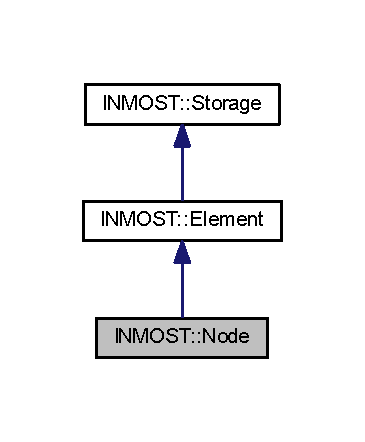
\includegraphics[width=175pt]{classINMOST_1_1Node__inherit__graph}
\end{center}
\end{figure}


Collaboration diagram for I\-N\-M\-O\-S\-T\-:\-:Node\-:\nopagebreak
\begin{figure}[H]
\begin{center}
\leavevmode
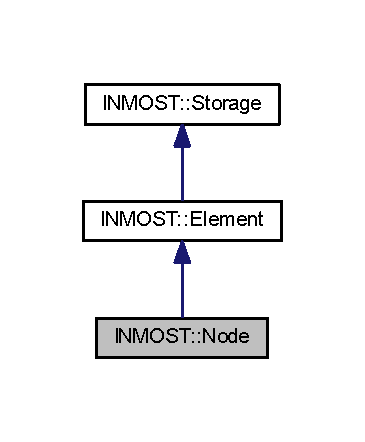
\includegraphics[width=175pt]{classINMOST_1_1Node__coll__graph}
\end{center}
\end{figure}
\subsection*{Public Member Functions}
\begin{DoxyCompactItemize}
\item 
\hypertarget{classINMOST_1_1Node_a3fc491ada3dc479780d467ee6cdb80ab}{{\bfseries Node} (const \hyperlink{classINMOST_1_1Node}{Node} \&other)}\label{classINMOST_1_1Node_a3fc491ada3dc479780d467ee6cdb80ab}

\item 
\hypertarget{classINMOST_1_1Node_ac5ddbc31a3ec69a4bb950f62b72e880b}{{\bfseries Node} (\hyperlink{classINMOST_1_1Mesh}{Mesh} $\ast$m, Handle\-Type h)}\label{classINMOST_1_1Node_ac5ddbc31a3ec69a4bb950f62b72e880b}

\item 
\hypertarget{classINMOST_1_1Node_a9c2c4cafdf456a58d02dc58b914ae294}{{\bfseries Node} (\hyperlink{classINMOST_1_1Mesh}{Mesh} $\ast$m, Handle\-Type $\ast$h)}\label{classINMOST_1_1Node_a9c2c4cafdf456a58d02dc58b914ae294}

\item 
\hypertarget{classINMOST_1_1Node_a66f15cc56dd523d7e445bf2daa4619c3}{\hyperlink{classINMOST_1_1Node}{Node} \& {\bfseries operator=} (\hyperlink{classINMOST_1_1Node}{Node} const \&other)}\label{classINMOST_1_1Node_a66f15cc56dd523d7e445bf2daa4619c3}

\item 
\hypertarget{classINMOST_1_1Node_a8a795b182d86d10bf78589a200d38e93}{\hyperlink{classINMOST_1_1Node}{Node} $\ast$ {\bfseries operator-\/$>$} ()}\label{classINMOST_1_1Node_a8a795b182d86d10bf78589a200d38e93}

\item 
\hypertarget{classINMOST_1_1Node_aabde896f896f372a6c6c0076716bb599}{const \hyperlink{classINMOST_1_1Node}{Node} $\ast$ {\bfseries operator-\/$>$} () const }\label{classINMOST_1_1Node_aabde896f896f372a6c6c0076716bb599}

\item 
\hypertarget{classINMOST_1_1Node_aecea484b041833ddff1635e4823cd0f2}{\hyperlink{classINMOST_1_1Node}{Node} \& {\bfseries self} ()}\label{classINMOST_1_1Node_aecea484b041833ddff1635e4823cd0f2}

\item 
\hypertarget{classINMOST_1_1Node_ab61e3edc72e68dd7c05a76ae0a9b8b6e}{const \hyperlink{classINMOST_1_1Node}{Node} \& {\bfseries self} () const }\label{classINMOST_1_1Node_ab61e3edc72e68dd7c05a76ae0a9b8b6e}

\item 
\hyperlink{classINMOST_1_1ElementArray}{Element\-Array}$<$ \hyperlink{classINMOST_1_1Edge}{Edge} $>$ \hyperlink{classINMOST_1_1Node_a43ca7289620b6df3347a1d5622350edb}{get\-Edges} () const 
\begin{DoxyCompactList}\small\item\em Retrieve all the edges of the element. \end{DoxyCompactList}\item 
\hyperlink{classINMOST_1_1ElementArray}{Element\-Array}$<$ \hyperlink{classINMOST_1_1Face}{Face} $>$ \hyperlink{classINMOST_1_1Node_a75d85d68fcd08f7d7f54a14d017bfbe2}{get\-Faces} () const 
\begin{DoxyCompactList}\small\item\em Retrieve all the faces of the element. \end{DoxyCompactList}\item 
\hyperlink{classINMOST_1_1ElementArray}{Element\-Array}$<$ \hyperlink{classINMOST_1_1Cell}{Cell} $>$ \hyperlink{classINMOST_1_1Node_a50abc7d16b296a9f6a2e1211dfb1d35a}{get\-Cells} () const 
\begin{DoxyCompactList}\small\item\em Return all the cells of the element. \end{DoxyCompactList}\item 
\hypertarget{classINMOST_1_1Node_a72e9d75a6afd913bf5f8463eb032948e}{\hyperlink{classINMOST_1_1ElementArray}{Element\-Array}$<$ \hyperlink{classINMOST_1_1Edge}{Edge} $>$ {\bfseries get\-Edges} (Marker\-Type mask, bool invert\-\_\-mask=false) const }\label{classINMOST_1_1Node_a72e9d75a6afd913bf5f8463eb032948e}

\item 
\hypertarget{classINMOST_1_1Node_a0174b70bae7e1959f18ff510fb736b89}{\hyperlink{classINMOST_1_1ElementArray}{Element\-Array}$<$ \hyperlink{classINMOST_1_1Face}{Face} $>$ {\bfseries get\-Faces} (Marker\-Type mask, bool invert\-\_\-mask=false) const }\label{classINMOST_1_1Node_a0174b70bae7e1959f18ff510fb736b89}

\item 
\hypertarget{classINMOST_1_1Node_ab2356978740c0fb34ad3e28b0a3251c2}{\hyperlink{classINMOST_1_1ElementArray}{Element\-Array}$<$ \hyperlink{classINMOST_1_1Cell}{Cell} $>$ {\bfseries get\-Cells} (Marker\-Type mask, bool invert\-\_\-mask=false) const }\label{classINMOST_1_1Node_ab2356978740c0fb34ad3e28b0a3251c2}

\item 
\hypertarget{classINMOST_1_1Node_aa309c3659f9c5c726ac2bf552a3f1963}{\hyperlink{classINMOST_1_1Storage_a430e5358d435befb38169beef593527e}{Storage\-::real\-\_\-array} {\bfseries Coords} () const }\label{classINMOST_1_1Node_aa309c3659f9c5c726ac2bf552a3f1963}

\end{DoxyCompactItemize}
\subsection*{Additional Inherited Members}


\subsection{Member Function Documentation}
\hypertarget{classINMOST_1_1Node_a50abc7d16b296a9f6a2e1211dfb1d35a}{\index{I\-N\-M\-O\-S\-T\-::\-Node@{I\-N\-M\-O\-S\-T\-::\-Node}!get\-Cells@{get\-Cells}}
\index{get\-Cells@{get\-Cells}!INMOST::Node@{I\-N\-M\-O\-S\-T\-::\-Node}}
\subsubsection[{get\-Cells}]{\setlength{\rightskip}{0pt plus 5cm}{\bf Element\-Array}$<${\bf Cell}$>$ I\-N\-M\-O\-S\-T\-::\-Node\-::get\-Cells (
\begin{DoxyParamCaption}
{}
\end{DoxyParamCaption}
) const\hspace{0.3cm}{\ttfamily [virtual]}}}\label{classINMOST_1_1Node_a50abc7d16b296a9f6a2e1211dfb1d35a}


Return all the cells of the element. 

For a node returns unordered set of cells.

For an edge returns unordered set of cells.

For a face returns a pair of cells. In the case Face\-::\-Check\-Normal\-Orientation returns true then the normal points from the first cell to the second and in oppisite direction otherwise.

For a cell returns itself.

\begin{DoxyReturn}{Returns}
array of elements 
\end{DoxyReturn}
\begin{DoxySeeAlso}{See Also}
Face\-::\-Face\-Oriented\-Outside 
\end{DoxySeeAlso}


Reimplemented from \hyperlink{classINMOST_1_1Element_aa90ec6b1e297fb9c1322b5558ccb7e2d}{I\-N\-M\-O\-S\-T\-::\-Element}.

\hypertarget{classINMOST_1_1Node_a43ca7289620b6df3347a1d5622350edb}{\index{I\-N\-M\-O\-S\-T\-::\-Node@{I\-N\-M\-O\-S\-T\-::\-Node}!get\-Edges@{get\-Edges}}
\index{get\-Edges@{get\-Edges}!INMOST::Node@{I\-N\-M\-O\-S\-T\-::\-Node}}
\subsubsection[{get\-Edges}]{\setlength{\rightskip}{0pt plus 5cm}{\bf Element\-Array}$<${\bf Edge}$>$ I\-N\-M\-O\-S\-T\-::\-Node\-::get\-Edges (
\begin{DoxyParamCaption}
{}
\end{DoxyParamCaption}
) const\hspace{0.3cm}{\ttfamily [virtual]}}}\label{classINMOST_1_1Node_a43ca7289620b6df3347a1d5622350edb}


Retrieve all the edges of the element. 

For a node returns unordered set of edges.

For an edge returns itself.

For a face returns ordered set of edges.

For a cell returns unordered set of edges.

\begin{DoxyReturn}{Returns}
array of elements 
\end{DoxyReturn}


Reimplemented from \hyperlink{classINMOST_1_1Element_a3ba56a19eeeb283864a006b0744fac4e}{I\-N\-M\-O\-S\-T\-::\-Element}.

\hypertarget{classINMOST_1_1Node_a75d85d68fcd08f7d7f54a14d017bfbe2}{\index{I\-N\-M\-O\-S\-T\-::\-Node@{I\-N\-M\-O\-S\-T\-::\-Node}!get\-Faces@{get\-Faces}}
\index{get\-Faces@{get\-Faces}!INMOST::Node@{I\-N\-M\-O\-S\-T\-::\-Node}}
\subsubsection[{get\-Faces}]{\setlength{\rightskip}{0pt plus 5cm}{\bf Element\-Array}$<${\bf Face}$>$ I\-N\-M\-O\-S\-T\-::\-Node\-::get\-Faces (
\begin{DoxyParamCaption}
{}
\end{DoxyParamCaption}
) const\hspace{0.3cm}{\ttfamily [virtual]}}}\label{classINMOST_1_1Node_a75d85d68fcd08f7d7f54a14d017bfbe2}


Retrieve all the faces of the element. 

For a node returns unordered set of faces.

For an edge returns unordered set of faces.

For a face returns itself.

For a cell return ordered set of faces. The order of faces in the cell is preserved from the first creation.

\begin{DoxyReturn}{Returns}
array of elements 
\end{DoxyReturn}


Reimplemented from \hyperlink{classINMOST_1_1Element_a2d9cc22d44f8d70c5b2876d84be6dfa5}{I\-N\-M\-O\-S\-T\-::\-Element}.



The documentation for this class was generated from the following file\-:\begin{DoxyCompactItemize}
\item 
inmost\-\_\-mesh.\-h\end{DoxyCompactItemize}

\hypertarget{classINMOST_1_1Solver_1_1OrderInfo}{\section{I\-N\-M\-O\-S\-T\-:\-:Solver\-:\-:Order\-Info Class Reference}
\label{classINMOST_1_1Solver_1_1OrderInfo}\index{I\-N\-M\-O\-S\-T\-::\-Solver\-::\-Order\-Info@{I\-N\-M\-O\-S\-T\-::\-Solver\-::\-Order\-Info}}
}


Base class for low level operations with objects of \hyperlink{classINMOST_1_1Solver}{Solver} class.  




{\ttfamily \#include $<$inmost\-\_\-solver.\-h$>$}

\subsection*{Public Member Functions}
\begin{DoxyCompactItemize}
\item 
\hypertarget{classINMOST_1_1Solver_1_1OrderInfo_a39cb3da0f477eebc9742377ab0e451cc}{void {\bfseries Clear} ()}\label{classINMOST_1_1Solver_1_1OrderInfo_a39cb3da0f477eebc9742377ab0e451cc}

\item 
\hypertarget{classINMOST_1_1Solver_1_1OrderInfo_a7a2e4998859c13bd156d40ab02c4d099}{bool \& \hyperlink{classINMOST_1_1Solver_1_1OrderInfo_a7a2e4998859c13bd156d40ab02c4d099}{Have\-Matrix} ()}\label{classINMOST_1_1Solver_1_1OrderInfo_a7a2e4998859c13bd156d40ab02c4d099}

\begin{DoxyCompactList}\small\item\em Return true if \hyperlink{classINMOST_1_1Solver_1_1Matrix}{Matrix} data have already been specified. \end{DoxyCompactList}\item 
\hypertarget{classINMOST_1_1Solver_1_1OrderInfo_a85ac0fe0f430301dab083aff8e241873}{{\bfseries Order\-Info} (const \hyperlink{classINMOST_1_1Solver_1_1OrderInfo}{Order\-Info} \&other)}\label{classINMOST_1_1Solver_1_1OrderInfo_a85ac0fe0f430301dab083aff8e241873}

\item 
\hypertarget{classINMOST_1_1Solver_1_1OrderInfo_a3d57307d3179f786d8a6fdc4948bc03b}{\hyperlink{classINMOST_1_1Solver_1_1OrderInfo}{Order\-Info} \& {\bfseries operator=} (\hyperlink{classINMOST_1_1Solver_1_1OrderInfo}{Order\-Info} const \&other)}\label{classINMOST_1_1Solver_1_1OrderInfo_a3d57307d3179f786d8a6fdc4948bc03b}

\item 
void \hyperlink{classINMOST_1_1Solver_1_1OrderInfo_a24d9af6294ae5f25d3eec4b7833108b6}{Prepare\-Matrix} (\hyperlink{classINMOST_1_1Solver_1_1Matrix}{Matrix} \&m, I\-N\-M\-O\-S\-T\-\_\-\-D\-A\-T\-A\-\_\-\-E\-N\-U\-M\-\_\-\-T\-Y\-P\-E overlap)
\begin{DoxyCompactList}\small\item\em Prepare parallel state of the \hyperlink{classINMOST_1_1Solver_1_1Matrix}{Matrix} with specified overlap size. \end{DoxyCompactList}\item 
\hypertarget{classINMOST_1_1Solver_1_1OrderInfo_ac56c713ddc7621e7125ef4ffe50ae281}{void \hyperlink{classINMOST_1_1Solver_1_1OrderInfo_ac56c713ddc7621e7125ef4ffe50ae281}{Restore\-Matrix} (\hyperlink{classINMOST_1_1Solver_1_1Matrix}{Matrix} \&m)}\label{classINMOST_1_1Solver_1_1OrderInfo_ac56c713ddc7621e7125ef4ffe50ae281}

\begin{DoxyCompactList}\small\item\em Restore initial nonparallel state of the \hyperlink{classINMOST_1_1Solver_1_1Matrix}{Matrix} with no overlap. \end{DoxyCompactList}\item 
\hypertarget{classINMOST_1_1Solver_1_1OrderInfo_ac5e96200d538f423e778f72fdde35501}{void \hyperlink{classINMOST_1_1Solver_1_1OrderInfo_ac5e96200d538f423e778f72fdde35501}{Prepare\-Vector} (\hyperlink{classINMOST_1_1Solver_1_1Vector}{Vector} \&v) const }\label{classINMOST_1_1Solver_1_1OrderInfo_ac5e96200d538f423e778f72fdde35501}

\begin{DoxyCompactList}\small\item\em Prepare parallel state of the \hyperlink{classINMOST_1_1Solver_1_1Vector}{Vector}. \end{DoxyCompactList}\item 
\hypertarget{classINMOST_1_1Solver_1_1OrderInfo_ac01e678d820b3461f6efedbc2adff276}{void \hyperlink{classINMOST_1_1Solver_1_1OrderInfo_ac01e678d820b3461f6efedbc2adff276}{Restore\-Vector} (\hyperlink{classINMOST_1_1Solver_1_1Vector}{Vector} \&v) const }\label{classINMOST_1_1Solver_1_1OrderInfo_ac01e678d820b3461f6efedbc2adff276}

\begin{DoxyCompactList}\small\item\em Restore initial nonparallel state of the \hyperlink{classINMOST_1_1Solver_1_1Vector}{Vector}. \end{DoxyCompactList}\item 
\hypertarget{classINMOST_1_1Solver_1_1OrderInfo_a620b59195a4bfa6a742e63d926b887a6}{I\-N\-M\-O\-S\-T\-\_\-\-D\-A\-T\-A\-\_\-\-E\-N\-U\-M\-\_\-\-T\-Y\-P\-E \hyperlink{classINMOST_1_1Solver_1_1OrderInfo_a620b59195a4bfa6a742e63d926b887a6}{Get\-Processor} (I\-N\-M\-O\-S\-T\-\_\-\-D\-A\-T\-A\-\_\-\-E\-N\-U\-M\-\_\-\-T\-Y\-P\-E gind) const }\label{classINMOST_1_1Solver_1_1OrderInfo_a620b59195a4bfa6a742e63d926b887a6}

\begin{DoxyCompactList}\small\item\em Retrieve the processor number by binary search for the specified global index. \end{DoxyCompactList}\item 
\hypertarget{classINMOST_1_1Solver_1_1OrderInfo_a4ce42a0cb98cef16a89ad959009f6abd}{void {\bfseries Get\-Overlap\-Region} (I\-N\-M\-O\-S\-T\-\_\-\-D\-A\-T\-A\-\_\-\-E\-N\-U\-M\-\_\-\-T\-Y\-P\-E proc, I\-N\-M\-O\-S\-T\-\_\-\-D\-A\-T\-A\-\_\-\-E\-N\-U\-M\-\_\-\-T\-Y\-P\-E \&mbeg, I\-N\-M\-O\-S\-T\-\_\-\-D\-A\-T\-A\-\_\-\-E\-N\-U\-M\-\_\-\-T\-Y\-P\-E \&mend) const }\label{classINMOST_1_1Solver_1_1OrderInfo_a4ce42a0cb98cef16a89ad959009f6abd}

\item 
\hypertarget{classINMOST_1_1Solver_1_1OrderInfo_a22fe66e8bb6198d67bdd7e97eee4fe23}{void \hyperlink{classINMOST_1_1Solver_1_1OrderInfo_a22fe66e8bb6198d67bdd7e97eee4fe23}{Get\-Local\-Region} (I\-N\-M\-O\-S\-T\-\_\-\-D\-A\-T\-A\-\_\-\-E\-N\-U\-M\-\_\-\-T\-Y\-P\-E proc, I\-N\-M\-O\-S\-T\-\_\-\-D\-A\-T\-A\-\_\-\-E\-N\-U\-M\-\_\-\-T\-Y\-P\-E \&mbeg, I\-N\-M\-O\-S\-T\-\_\-\-D\-A\-T\-A\-\_\-\-E\-N\-U\-M\-\_\-\-T\-Y\-P\-E \&mend) const }\label{classINMOST_1_1Solver_1_1OrderInfo_a22fe66e8bb6198d67bdd7e97eee4fe23}

\begin{DoxyCompactList}\small\item\em Get the local index region for the specified process. \end{DoxyCompactList}\item 
\hypertarget{classINMOST_1_1Solver_1_1OrderInfo_a03437ef8f15cef652ada3a6c401bdfcd}{void \hyperlink{classINMOST_1_1Solver_1_1OrderInfo_a03437ef8f15cef652ada3a6c401bdfcd}{Get\-Vector\-Region} (I\-N\-M\-O\-S\-T\-\_\-\-D\-A\-T\-A\-\_\-\-E\-N\-U\-M\-\_\-\-T\-Y\-P\-E \&mbeg, I\-N\-M\-O\-S\-T\-\_\-\-D\-A\-T\-A\-\_\-\-E\-N\-U\-M\-\_\-\-T\-Y\-P\-E \&mend) const }\label{classINMOST_1_1Solver_1_1OrderInfo_a03437ef8f15cef652ada3a6c401bdfcd}

\begin{DoxyCompactList}\small\item\em Get the local index region for the current process. \end{DoxyCompactList}\item 
\hypertarget{classINMOST_1_1Solver_1_1OrderInfo_a63c69e2e7e85de999627eb12a547a0c6}{I\-N\-M\-O\-S\-T\-\_\-\-D\-A\-T\-A\-\_\-\-E\-N\-U\-M\-\_\-\-T\-Y\-P\-E \hyperlink{classINMOST_1_1Solver_1_1OrderInfo_a63c69e2e7e85de999627eb12a547a0c6}{Get\-Rank} () const }\label{classINMOST_1_1Solver_1_1OrderInfo_a63c69e2e7e85de999627eb12a547a0c6}

\begin{DoxyCompactList}\small\item\em Get the rank of the current communicator, i.\-e. the current process index. \end{DoxyCompactList}\item 
\hypertarget{classINMOST_1_1Solver_1_1OrderInfo_abb1a4ca671c5d5e731926c300d597825}{I\-N\-M\-O\-S\-T\-\_\-\-D\-A\-T\-A\-\_\-\-E\-N\-U\-M\-\_\-\-T\-Y\-P\-E \hyperlink{classINMOST_1_1Solver_1_1OrderInfo_abb1a4ca671c5d5e731926c300d597825}{Get\-Size} () const }\label{classINMOST_1_1Solver_1_1OrderInfo_abb1a4ca671c5d5e731926c300d597825}

\begin{DoxyCompactList}\small\item\em Get the size of the current communicator, i.\-e. the total number of processes used. \end{DoxyCompactList}\item 
\hypertarget{classINMOST_1_1Solver_1_1OrderInfo_a76c34bb3769aa0f8b29d0a9bb4f05d0c}{void \hyperlink{classINMOST_1_1Solver_1_1OrderInfo_a76c34bb3769aa0f8b29d0a9bb4f05d0c}{Update} (\hyperlink{classINMOST_1_1Solver_1_1Vector}{Vector} \&x)}\label{classINMOST_1_1Solver_1_1OrderInfo_a76c34bb3769aa0f8b29d0a9bb4f05d0c}

\begin{DoxyCompactList}\small\item\em Update the shared data in parallel vector. \end{DoxyCompactList}\item 
\hypertarget{classINMOST_1_1Solver_1_1OrderInfo_a4576eab65fafa6986f46161444e47850}{void \hyperlink{classINMOST_1_1Solver_1_1OrderInfo_a4576eab65fafa6986f46161444e47850}{Accumulate} (\hyperlink{classINMOST_1_1Solver_1_1Vector}{Vector} \&x)}\label{classINMOST_1_1Solver_1_1OrderInfo_a4576eab65fafa6986f46161444e47850}

\begin{DoxyCompactList}\small\item\em Sum shared values in parallel vector. \end{DoxyCompactList}\item 
\hypertarget{classINMOST_1_1Solver_1_1OrderInfo_af82028af97d514f9811d21a5b58ae9e9}{void \hyperlink{classINMOST_1_1Solver_1_1OrderInfo_af82028af97d514f9811d21a5b58ae9e9}{Integrate} (I\-N\-M\-O\-S\-T\-\_\-\-D\-A\-T\-A\-\_\-\-R\-E\-A\-L\-\_\-\-T\-Y\-P\-E $\ast$inout, I\-N\-M\-O\-S\-T\-\_\-\-D\-A\-T\-A\-\_\-\-E\-N\-U\-M\-\_\-\-T\-Y\-P\-E num) const }\label{classINMOST_1_1Solver_1_1OrderInfo_af82028af97d514f9811d21a5b58ae9e9}

\begin{DoxyCompactList}\small\item\em Get the sum of num elements of real array on all processes. \end{DoxyCompactList}\item 
\hypertarget{classINMOST_1_1Solver_1_1OrderInfo_a95d7134a518336c36025e18171eafb05}{I\-N\-M\-O\-S\-T\-\_\-\-M\-P\-I\-\_\-\-Comm \hyperlink{classINMOST_1_1Solver_1_1OrderInfo_a95d7134a518336c36025e18171eafb05}{Get\-Comm} () const }\label{classINMOST_1_1Solver_1_1OrderInfo_a95d7134a518336c36025e18171eafb05}

\begin{DoxyCompactList}\small\item\em Get the communicator which the solver is associated with. \end{DoxyCompactList}\item 
\hypertarget{classINMOST_1_1Solver_1_1OrderInfo_a0e4e243c601d87a4be072c2fc8c1a3c9}{I\-N\-M\-O\-S\-T\-\_\-\-M\-P\-I\-\_\-\-Request $\ast$ {\bfseries Get\-Send\-Requests} ()}\label{classINMOST_1_1Solver_1_1OrderInfo_a0e4e243c601d87a4be072c2fc8c1a3c9}

\item 
\hypertarget{classINMOST_1_1Solver_1_1OrderInfo_a9fb17df8429be00a1a9489d44a04645e}{I\-N\-M\-O\-S\-T\-\_\-\-M\-P\-I\-\_\-\-Request $\ast$ {\bfseries Get\-Recv\-Requests} ()}\label{classINMOST_1_1Solver_1_1OrderInfo_a9fb17df8429be00a1a9489d44a04645e}

\item 
\hypertarget{classINMOST_1_1Solver_1_1OrderInfo_a3f0bac5fba6d238cb22a76c2094a5f48}{I\-N\-M\-O\-S\-T\-\_\-\-D\-A\-T\-A\-\_\-\-E\-N\-U\-M\-\_\-\-T\-Y\-P\-E {\bfseries Get\-Send\-Requests\-Size} ()}\label{classINMOST_1_1Solver_1_1OrderInfo_a3f0bac5fba6d238cb22a76c2094a5f48}

\item 
\hypertarget{classINMOST_1_1Solver_1_1OrderInfo_ae766d3d64dc46603feb600e1f19105c5}{I\-N\-M\-O\-S\-T\-\_\-\-D\-A\-T\-A\-\_\-\-E\-N\-U\-M\-\_\-\-T\-Y\-P\-E {\bfseries Get\-Recv\-Requests\-Size} ()}\label{classINMOST_1_1Solver_1_1OrderInfo_ae766d3d64dc46603feb600e1f19105c5}

\item 
\hypertarget{classINMOST_1_1Solver_1_1OrderInfo_ad3df60e1a4c9e016aef33a800e048dce}{I\-N\-M\-O\-S\-T\-\_\-\-D\-A\-T\-A\-\_\-\-E\-N\-U\-M\-\_\-\-T\-Y\-P\-E $\ast$ {\bfseries Get\-Send\-Exchange\-Array} ()}\label{classINMOST_1_1Solver_1_1OrderInfo_ad3df60e1a4c9e016aef33a800e048dce}

\item 
\hypertarget{classINMOST_1_1Solver_1_1OrderInfo_acb8c8c157fbdb8609047cad5a18407ea}{I\-N\-M\-O\-S\-T\-\_\-\-D\-A\-T\-A\-\_\-\-E\-N\-U\-M\-\_\-\-T\-Y\-P\-E {\bfseries Get\-Send\-Exchange\-Size} ()}\label{classINMOST_1_1Solver_1_1OrderInfo_acb8c8c157fbdb8609047cad5a18407ea}

\item 
\hypertarget{classINMOST_1_1Solver_1_1OrderInfo_a90ba99d91a554c149d20f1cbbcb9afee}{I\-N\-M\-O\-S\-T\-\_\-\-D\-A\-T\-A\-\_\-\-E\-N\-U\-M\-\_\-\-T\-Y\-P\-E $\ast$ {\bfseries Get\-Recv\-Exchange\-Array} ()}\label{classINMOST_1_1Solver_1_1OrderInfo_a90ba99d91a554c149d20f1cbbcb9afee}

\item 
\hypertarget{classINMOST_1_1Solver_1_1OrderInfo_a786492332f92c61da93e69864e173f4a}{I\-N\-M\-O\-S\-T\-\_\-\-D\-A\-T\-A\-\_\-\-E\-N\-U\-M\-\_\-\-T\-Y\-P\-E {\bfseries Get\-Recv\-Exchange\-Size} ()}\label{classINMOST_1_1Solver_1_1OrderInfo_a786492332f92c61da93e69864e173f4a}

\item 
\hypertarget{classINMOST_1_1Solver_1_1OrderInfo_a9dd49ffce6b6008212c97f9c93ce8d4e}{I\-N\-M\-O\-S\-T\-\_\-\-D\-A\-T\-A\-\_\-\-R\-E\-A\-L\-\_\-\-T\-Y\-P\-E \hyperlink{classINMOST_1_1Solver_1_1OrderInfo_a9dd49ffce6b6008212c97f9c93ce8d4e}{Scalar\-Prod} (\hyperlink{classINMOST_1_1Solver_1_1Vector}{Vector} const \&left, \hyperlink{classINMOST_1_1Solver_1_1Vector}{Vector} const \&right, I\-N\-M\-O\-S\-T\-\_\-\-D\-A\-T\-A\-\_\-\-E\-N\-U\-M\-\_\-\-T\-Y\-P\-E index\-\_\-begin, I\-N\-M\-O\-S\-T\-\_\-\-D\-A\-T\-A\-\_\-\-E\-N\-U\-M\-\_\-\-T\-Y\-P\-E index\-\_\-end) const }\label{classINMOST_1_1Solver_1_1OrderInfo_a9dd49ffce6b6008212c97f9c93ce8d4e}

\begin{DoxyCompactList}\small\item\em Get the scalar product of the specified interval of the distributed vector. \end{DoxyCompactList}\end{DoxyCompactItemize}


\subsection{Detailed Description}
Base class for low level operations with objects of \hyperlink{classINMOST_1_1Solver}{Solver} class. 

\subsection{Member Function Documentation}
\hypertarget{classINMOST_1_1Solver_1_1OrderInfo_a24d9af6294ae5f25d3eec4b7833108b6}{\index{I\-N\-M\-O\-S\-T\-::\-Solver\-::\-Order\-Info@{I\-N\-M\-O\-S\-T\-::\-Solver\-::\-Order\-Info}!Prepare\-Matrix@{Prepare\-Matrix}}
\index{Prepare\-Matrix@{Prepare\-Matrix}!INMOST::Solver::OrderInfo@{I\-N\-M\-O\-S\-T\-::\-Solver\-::\-Order\-Info}}
\subsubsection[{Prepare\-Matrix}]{\setlength{\rightskip}{0pt plus 5cm}void I\-N\-M\-O\-S\-T\-::\-Solver\-::\-Order\-Info\-::\-Prepare\-Matrix (
\begin{DoxyParamCaption}
\item[{{\bf Matrix} \&}]{m, }
\item[{I\-N\-M\-O\-S\-T\-\_\-\-D\-A\-T\-A\-\_\-\-E\-N\-U\-M\-\_\-\-T\-Y\-P\-E}]{overlap}
\end{DoxyParamCaption}
)}}\label{classINMOST_1_1Solver_1_1OrderInfo_a24d9af6294ae5f25d3eec4b7833108b6}


Prepare parallel state of the \hyperlink{classINMOST_1_1Solver_1_1Matrix}{Matrix} with specified overlap size. 

This state of the matrix can be used, for instance, to construct the preconditioner for Additive Swartz method. 
\begin{DoxyParams}{Parameters}
{\em m} & \hyperlink{classINMOST_1_1Solver_1_1Matrix}{Matrix} to be expanded. \\
\hline
{\em overlap} & Overlap size, viz. the number of overlap layers. \\
\hline
\end{DoxyParams}


The documentation for this class was generated from the following file\-:\begin{DoxyCompactItemize}
\item 
inmost\-\_\-solver.\-h\end{DoxyCompactItemize}

\hypertarget{classINMOST_1_1Partitioner}{\section{I\-N\-M\-O\-S\-T\-:\-:Partitioner Class Reference}
\label{classINMOST_1_1Partitioner}\index{I\-N\-M\-O\-S\-T\-::\-Partitioner@{I\-N\-M\-O\-S\-T\-::\-Partitioner}}
}


Main class to modify or improve the mesh distribution for better load balancing.  




{\ttfamily \#include $<$inmost\-\_\-partitioner.\-h$>$}

\subsection*{Public Types}
\begin{DoxyCompactItemize}
\item 
enum \hyperlink{classINMOST_1_1Partitioner_a0699b96f7945e283398750d585eca311}{Type} \{ \\*
\hyperlink{classINMOST_1_1Partitioner_a0699b96f7945e283398750d585eca311ad68b743147cac9faa8500a57e7f22bb0}{Zoltan\-\_\-\-Parmetis}, 
\hyperlink{classINMOST_1_1Partitioner_a0699b96f7945e283398750d585eca311accde25f216216d856af62a7f0540ee3a}{Zoltan\-\_\-\-Scotch}, 
\hyperlink{classINMOST_1_1Partitioner_a0699b96f7945e283398750d585eca311a8d727bd538073eb973d5daf67c6e807b}{Zoltan\-\_\-\-P\-H\-G}, 
\hyperlink{classINMOST_1_1Partitioner_a0699b96f7945e283398750d585eca311a39286e4771ba65760112a1332b584b7d}{Zoltan\-\_\-\-R\-C\-B}, 
\\*
\hyperlink{classINMOST_1_1Partitioner_a0699b96f7945e283398750d585eca311aa113ffce71bea31673400f4ed6f3f68c}{Zoltan\-\_\-\-R\-I\-B}, 
\hyperlink{classINMOST_1_1Partitioner_a0699b96f7945e283398750d585eca311a01cc8e6db082dc0bcdc19a8d5d0ea2e2}{Zoltan\-\_\-\-H\-S\-F\-C}, 
\hyperlink{classINMOST_1_1Partitioner_a0699b96f7945e283398750d585eca311a32d02a7da6210f8213944fb9c351a778}{Parmetis}, 
\hyperlink{classINMOST_1_1Partitioner_a0699b96f7945e283398750d585eca311a4411b1b230aac80bb4ce95d0000ff336}{Inner\-\_\-\-R\-C\-M}
 \}
\begin{DoxyCompactList}\small\item\em Type of the \hyperlink{classINMOST_1_1Partitioner}{Partitioner} can be currently used in this version of I\-N\-M\-O\-S\-T. \end{DoxyCompactList}\item 
enum \hyperlink{classINMOST_1_1Partitioner_a0a4053a79855f16dbb53c13b39bc75c3}{Action} \{ \hyperlink{classINMOST_1_1Partitioner_a0a4053a79855f16dbb53c13b39bc75c3ad747444c0947b3a6a697efd54ae42771}{Partition}, 
\hyperlink{classINMOST_1_1Partitioner_a0a4053a79855f16dbb53c13b39bc75c3ae667d6f0560495262c0010866080eff8}{Repartition}, 
\hyperlink{classINMOST_1_1Partitioner_a0a4053a79855f16dbb53c13b39bc75c3a2d75221ee80b15356021e80283da41d6}{Refine}
 \}
\end{DoxyCompactItemize}
\subsection*{Public Member Functions}
\begin{DoxyCompactItemize}
\item 
\hypertarget{classINMOST_1_1Partitioner_a3aeebab26c4e59b6d4207f2066883283}{\hyperlink{classINMOST_1_1Partitioner_a3aeebab26c4e59b6d4207f2066883283}{Partitioner} (\hyperlink{classINMOST_1_1Mesh}{Mesh} $\ast$m)}\label{classINMOST_1_1Partitioner_a3aeebab26c4e59b6d4207f2066883283}

\begin{DoxyCompactList}\small\item\em The default constructor of the partitioner for the specified mesh. \end{DoxyCompactList}\item 
\hypertarget{classINMOST_1_1Partitioner_a078dfb29545637a627e830c50749c36f}{{\bfseries Partitioner} (const \hyperlink{classINMOST_1_1Partitioner}{Partitioner} \&other)}\label{classINMOST_1_1Partitioner_a078dfb29545637a627e830c50749c36f}

\item 
\hypertarget{classINMOST_1_1Partitioner_a3ef0bfba7413f977879176dba9be6c35}{\hyperlink{classINMOST_1_1Partitioner}{Partitioner} \& {\bfseries operator=} (\hyperlink{classINMOST_1_1Partitioner}{Partitioner} const \&other)}\label{classINMOST_1_1Partitioner_a3ef0bfba7413f977879176dba9be6c35}

\item 
void \hyperlink{classINMOST_1_1Partitioner_aafc007c0dce3a6cde19d3de8afd0bb7f}{Evaluate} ()
\begin{DoxyCompactList}\small\item\em Evaluate the earlier specified partitioner. \end{DoxyCompactList}\item 
void \hyperlink{classINMOST_1_1Partitioner_aec7573d66aaf19911e990561b47236eb}{Set\-Method} (enum \hyperlink{classINMOST_1_1Partitioner_a0699b96f7945e283398750d585eca311}{Type} t, enum \hyperlink{classINMOST_1_1Partitioner_a0a4053a79855f16dbb53c13b39bc75c3}{Action} a=\hyperlink{classINMOST_1_1Partitioner_a0a4053a79855f16dbb53c13b39bc75c3ae667d6f0560495262c0010866080eff8}{Repartition})
\begin{DoxyCompactList}\small\item\em Set the partitioner method to be used. \end{DoxyCompactList}\item 
\hypertarget{classINMOST_1_1Partitioner_a48e793e9e60e7438b2f5504f9bf5bccd}{void \hyperlink{classINMOST_1_1Partitioner_a48e793e9e60e7438b2f5504f9bf5bccd}{Set\-Weight} (\hyperlink{classINMOST_1_1Tag}{Tag} weight)}\label{classINMOST_1_1Partitioner_a48e793e9e60e7438b2f5504f9bf5bccd}

\begin{DoxyCompactList}\small\item\em Compute the specific weights for the selected partitioner. \end{DoxyCompactList}\item 
\hypertarget{classINMOST_1_1Partitioner_ae3a9cc78be5b685316e1eabb2cd00a79}{void \hyperlink{classINMOST_1_1Partitioner_ae3a9cc78be5b685316e1eabb2cd00a79}{Reset\-Weight} ()}\label{classINMOST_1_1Partitioner_ae3a9cc78be5b685316e1eabb2cd00a79}

\begin{DoxyCompactList}\small\item\em Reset the computed weights for the partitioner. \end{DoxyCompactList}\item 
\hypertarget{classINMOST_1_1Partitioner_a372a7b3650c770c8adc8769dba8793d9}{\hyperlink{classINMOST_1_1Mesh}{Mesh} $\ast$ \hyperlink{classINMOST_1_1Partitioner_a372a7b3650c770c8adc8769dba8793d9}{Get\-Mesh} ()}\label{classINMOST_1_1Partitioner_a372a7b3650c770c8adc8769dba8793d9}

\begin{DoxyCompactList}\small\item\em Get the \hyperlink{classINMOST_1_1Mesh}{Mesh} pointer for the current partitioner. \end{DoxyCompactList}\item 
\hypertarget{classINMOST_1_1Partitioner_a7ad2c7e955369ae57b40cd9433427c5b}{\hyperlink{classINMOST_1_1Tag}{Tag} \hyperlink{classINMOST_1_1Partitioner_a7ad2c7e955369ae57b40cd9433427c5b}{Get\-Weight} ()}\label{classINMOST_1_1Partitioner_a7ad2c7e955369ae57b40cd9433427c5b}

\begin{DoxyCompactList}\small\item\em Get the \hyperlink{classINMOST_1_1Tag}{Tag} of the computed weights for the current partitioner. \end{DoxyCompactList}\end{DoxyCompactItemize}
\subsection*{Static Public Member Functions}
\begin{DoxyCompactItemize}
\item 
static void \hyperlink{classINMOST_1_1Partitioner_a6499e92ff7f475573e1bc4b157b09573}{Initialize} (int $\ast$argc, char $\ast$$\ast$$\ast$argv)
\begin{DoxyCompactList}\small\item\em Initialize the use of partitioner. \end{DoxyCompactList}\item 
static void \hyperlink{classINMOST_1_1Partitioner_af9ff5247ee5d6dfa28e0fba266a1cb03}{Finalize} ()
\begin{DoxyCompactList}\small\item\em Finalize the use of partitioner. \end{DoxyCompactList}\end{DoxyCompactItemize}


\subsection{Detailed Description}
Main class to modify or improve the mesh distribution for better load balancing. 

\subsection{Member Enumeration Documentation}
\hypertarget{classINMOST_1_1Partitioner_a0a4053a79855f16dbb53c13b39bc75c3}{\index{I\-N\-M\-O\-S\-T\-::\-Partitioner@{I\-N\-M\-O\-S\-T\-::\-Partitioner}!Action@{Action}}
\index{Action@{Action}!INMOST::Partitioner@{I\-N\-M\-O\-S\-T\-::\-Partitioner}}
\subsubsection[{Action}]{\setlength{\rightskip}{0pt plus 5cm}enum {\bf I\-N\-M\-O\-S\-T\-::\-Partitioner\-::\-Action}}}\label{classINMOST_1_1Partitioner_a0a4053a79855f16dbb53c13b39bc75c3}
\begin{Desc}
\item[Enumerator]\par
\begin{description}
\index{Partition@{Partition}!I\-N\-M\-O\-S\-T\-::\-Partitioner@{I\-N\-M\-O\-S\-T\-::\-Partitioner}}\index{I\-N\-M\-O\-S\-T\-::\-Partitioner@{I\-N\-M\-O\-S\-T\-::\-Partitioner}!Partition@{Partition}}\item[{\em 
\hypertarget{classINMOST_1_1Partitioner_a0a4053a79855f16dbb53c13b39bc75c3ad747444c0947b3a6a697efd54ae42771}{Partition}\label{classINMOST_1_1Partitioner_a0a4053a79855f16dbb53c13b39bc75c3ad747444c0947b3a6a697efd54ae42771}
}]Partition \char`\"{}from scratch\char`\"{}, not taking into account the current mesh distribution. \index{Repartition@{Repartition}!I\-N\-M\-O\-S\-T\-::\-Partitioner@{I\-N\-M\-O\-S\-T\-::\-Partitioner}}\index{I\-N\-M\-O\-S\-T\-::\-Partitioner@{I\-N\-M\-O\-S\-T\-::\-Partitioner}!Repartition@{Repartition}}\item[{\em 
\hypertarget{classINMOST_1_1Partitioner_a0a4053a79855f16dbb53c13b39bc75c3ae667d6f0560495262c0010866080eff8}{Repartition}\label{classINMOST_1_1Partitioner_a0a4053a79855f16dbb53c13b39bc75c3ae667d6f0560495262c0010866080eff8}
}]Repartition the existing partition but try to stay close to the current mesh distribution. \index{Refine@{Refine}!I\-N\-M\-O\-S\-T\-::\-Partitioner@{I\-N\-M\-O\-S\-T\-::\-Partitioner}}\index{I\-N\-M\-O\-S\-T\-::\-Partitioner@{I\-N\-M\-O\-S\-T\-::\-Partitioner}!Refine@{Refine}}\item[{\em 
\hypertarget{classINMOST_1_1Partitioner_a0a4053a79855f16dbb53c13b39bc75c3a2d75221ee80b15356021e80283da41d6}{Refine}\label{classINMOST_1_1Partitioner_a0a4053a79855f16dbb53c13b39bc75c3a2d75221ee80b15356021e80283da41d6}
}]Refine the current partition assuming only small changes of mesh distribution. \end{description}
\end{Desc}
\hypertarget{classINMOST_1_1Partitioner_a0699b96f7945e283398750d585eca311}{\index{I\-N\-M\-O\-S\-T\-::\-Partitioner@{I\-N\-M\-O\-S\-T\-::\-Partitioner}!Type@{Type}}
\index{Type@{Type}!INMOST::Partitioner@{I\-N\-M\-O\-S\-T\-::\-Partitioner}}
\subsubsection[{Type}]{\setlength{\rightskip}{0pt plus 5cm}enum {\bf I\-N\-M\-O\-S\-T\-::\-Partitioner\-::\-Type}}}\label{classINMOST_1_1Partitioner_a0699b96f7945e283398750d585eca311}


Type of the \hyperlink{classINMOST_1_1Partitioner}{Partitioner} can be currently used in this version of I\-N\-M\-O\-S\-T. 

\begin{DoxySeeAlso}{See Also}
Zoltan\-: Parallel Partitioning, Load Balancing and Data-\/\-Management Services. \href{http://www.cs.sandia.gov/Zoltan/}{\tt http\-://www.\-cs.\-sandia.\-gov/\-Zoltan/} 

Par\-M\-E\-T\-I\-S\-: Parallel Graph Partitioning and Fill-\/reducing Matrix Ordering. \href{http://glaros.dtc.umn.edu/gkhome/metis/parmetis/overview}{\tt http\-://glaros.\-dtc.\-umn.\-edu/gkhome/metis/parmetis/overview} 
\end{DoxySeeAlso}
\begin{Desc}
\item[Enumerator]\par
\begin{description}
\index{Zoltan\-\_\-\-Parmetis@{Zoltan\-\_\-\-Parmetis}!I\-N\-M\-O\-S\-T\-::\-Partitioner@{I\-N\-M\-O\-S\-T\-::\-Partitioner}}\index{I\-N\-M\-O\-S\-T\-::\-Partitioner@{I\-N\-M\-O\-S\-T\-::\-Partitioner}!Zoltan\-\_\-\-Parmetis@{Zoltan\-\_\-\-Parmetis}}\item[{\em 
\hypertarget{classINMOST_1_1Partitioner_a0699b96f7945e283398750d585eca311ad68b743147cac9faa8500a57e7f22bb0}{Zoltan\-\_\-\-Parmetis}\label{classINMOST_1_1Partitioner_a0699b96f7945e283398750d585eca311ad68b743147cac9faa8500a57e7f22bb0}
}]Parmetis partitioner with the Zoltan package interface. \index{Zoltan\-\_\-\-Scotch@{Zoltan\-\_\-\-Scotch}!I\-N\-M\-O\-S\-T\-::\-Partitioner@{I\-N\-M\-O\-S\-T\-::\-Partitioner}}\index{I\-N\-M\-O\-S\-T\-::\-Partitioner@{I\-N\-M\-O\-S\-T\-::\-Partitioner}!Zoltan\-\_\-\-Scotch@{Zoltan\-\_\-\-Scotch}}\item[{\em 
\hypertarget{classINMOST_1_1Partitioner_a0699b96f7945e283398750d585eca311accde25f216216d856af62a7f0540ee3a}{Zoltan\-\_\-\-Scotch}\label{classINMOST_1_1Partitioner_a0699b96f7945e283398750d585eca311accde25f216216d856af62a7f0540ee3a}
}]Scotch partitioner with the Zoltan package interface. \index{Zoltan\-\_\-\-P\-H\-G@{Zoltan\-\_\-\-P\-H\-G}!I\-N\-M\-O\-S\-T\-::\-Partitioner@{I\-N\-M\-O\-S\-T\-::\-Partitioner}}\index{I\-N\-M\-O\-S\-T\-::\-Partitioner@{I\-N\-M\-O\-S\-T\-::\-Partitioner}!Zoltan\-\_\-\-P\-H\-G@{Zoltan\-\_\-\-P\-H\-G}}\item[{\em 
\hypertarget{classINMOST_1_1Partitioner_a0699b96f7945e283398750d585eca311a8d727bd538073eb973d5daf67c6e807b}{Zoltan\-\_\-\-P\-H\-G}\label{classINMOST_1_1Partitioner_a0699b96f7945e283398750d585eca311a8d727bd538073eb973d5daf67c6e807b}
}]Zoltan topology-\/based method using Partitioning of Hyper\-Graph. \index{Zoltan\-\_\-\-R\-C\-B@{Zoltan\-\_\-\-R\-C\-B}!I\-N\-M\-O\-S\-T\-::\-Partitioner@{I\-N\-M\-O\-S\-T\-::\-Partitioner}}\index{I\-N\-M\-O\-S\-T\-::\-Partitioner@{I\-N\-M\-O\-S\-T\-::\-Partitioner}!Zoltan\-\_\-\-R\-C\-B@{Zoltan\-\_\-\-R\-C\-B}}\item[{\em 
\hypertarget{classINMOST_1_1Partitioner_a0699b96f7945e283398750d585eca311a39286e4771ba65760112a1332b584b7d}{Zoltan\-\_\-\-R\-C\-B}\label{classINMOST_1_1Partitioner_a0699b96f7945e283398750d585eca311a39286e4771ba65760112a1332b584b7d}
}]Zoltan geometry-\/based method using Recursive Coordinate Bisection. \index{Zoltan\-\_\-\-R\-I\-B@{Zoltan\-\_\-\-R\-I\-B}!I\-N\-M\-O\-S\-T\-::\-Partitioner@{I\-N\-M\-O\-S\-T\-::\-Partitioner}}\index{I\-N\-M\-O\-S\-T\-::\-Partitioner@{I\-N\-M\-O\-S\-T\-::\-Partitioner}!Zoltan\-\_\-\-R\-I\-B@{Zoltan\-\_\-\-R\-I\-B}}\item[{\em 
\hypertarget{classINMOST_1_1Partitioner_a0699b96f7945e283398750d585eca311aa113ffce71bea31673400f4ed6f3f68c}{Zoltan\-\_\-\-R\-I\-B}\label{classINMOST_1_1Partitioner_a0699b96f7945e283398750d585eca311aa113ffce71bea31673400f4ed6f3f68c}
}]Zoltan geometry-\/based method using Recursive Inertial Bisection. \index{Zoltan\-\_\-\-H\-S\-F\-C@{Zoltan\-\_\-\-H\-S\-F\-C}!I\-N\-M\-O\-S\-T\-::\-Partitioner@{I\-N\-M\-O\-S\-T\-::\-Partitioner}}\index{I\-N\-M\-O\-S\-T\-::\-Partitioner@{I\-N\-M\-O\-S\-T\-::\-Partitioner}!Zoltan\-\_\-\-H\-S\-F\-C@{Zoltan\-\_\-\-H\-S\-F\-C}}\item[{\em 
\hypertarget{classINMOST_1_1Partitioner_a0699b96f7945e283398750d585eca311a01cc8e6db082dc0bcdc19a8d5d0ea2e2}{Zoltan\-\_\-\-H\-S\-F\-C}\label{classINMOST_1_1Partitioner_a0699b96f7945e283398750d585eca311a01cc8e6db082dc0bcdc19a8d5d0ea2e2}
}]Zoltan geometry-\/based method using Hilbert Space-\/\-Filling Curve partitioning. \index{Parmetis@{Parmetis}!I\-N\-M\-O\-S\-T\-::\-Partitioner@{I\-N\-M\-O\-S\-T\-::\-Partitioner}}\index{I\-N\-M\-O\-S\-T\-::\-Partitioner@{I\-N\-M\-O\-S\-T\-::\-Partitioner}!Parmetis@{Parmetis}}\item[{\em 
\hypertarget{classINMOST_1_1Partitioner_a0699b96f7945e283398750d585eca311a32d02a7da6210f8213944fb9c351a778}{Parmetis}\label{classINMOST_1_1Partitioner_a0699b96f7945e283398750d585eca311a32d02a7da6210f8213944fb9c351a778}
}]Parmetis partitioner with the original interface. \index{Inner\-\_\-\-R\-C\-M@{Inner\-\_\-\-R\-C\-M}!I\-N\-M\-O\-S\-T\-::\-Partitioner@{I\-N\-M\-O\-S\-T\-::\-Partitioner}}\index{I\-N\-M\-O\-S\-T\-::\-Partitioner@{I\-N\-M\-O\-S\-T\-::\-Partitioner}!Inner\-\_\-\-R\-C\-M@{Inner\-\_\-\-R\-C\-M}}\item[{\em 
\hypertarget{classINMOST_1_1Partitioner_a0699b96f7945e283398750d585eca311a4411b1b230aac80bb4ce95d0000ff336}{Inner\-\_\-\-R\-C\-M}\label{classINMOST_1_1Partitioner_a0699b96f7945e283398750d585eca311a4411b1b230aac80bb4ce95d0000ff336}
}]Internal serial only partitioner based on the Reverse Cuthill–\-Mc\-Kee algorithm ordering. \end{description}
\end{Desc}


\subsection{Member Function Documentation}
\hypertarget{classINMOST_1_1Partitioner_aafc007c0dce3a6cde19d3de8afd0bb7f}{\index{I\-N\-M\-O\-S\-T\-::\-Partitioner@{I\-N\-M\-O\-S\-T\-::\-Partitioner}!Evaluate@{Evaluate}}
\index{Evaluate@{Evaluate}!INMOST::Partitioner@{I\-N\-M\-O\-S\-T\-::\-Partitioner}}
\subsubsection[{Evaluate}]{\setlength{\rightskip}{0pt plus 5cm}void I\-N\-M\-O\-S\-T\-::\-Partitioner\-::\-Evaluate (
\begin{DoxyParamCaption}
{}
\end{DoxyParamCaption}
)}}\label{classINMOST_1_1Partitioner_aafc007c0dce3a6cde19d3de8afd0bb7f}


Evaluate the earlier specified partitioner. 

\begin{DoxySeeAlso}{See Also}
\hyperlink{classINMOST_1_1Partitioner_aec7573d66aaf19911e990561b47236eb}{Partitioner\-::\-Set\-Method} 
\end{DoxySeeAlso}
\hypertarget{classINMOST_1_1Partitioner_af9ff5247ee5d6dfa28e0fba266a1cb03}{\index{I\-N\-M\-O\-S\-T\-::\-Partitioner@{I\-N\-M\-O\-S\-T\-::\-Partitioner}!Finalize@{Finalize}}
\index{Finalize@{Finalize}!INMOST::Partitioner@{I\-N\-M\-O\-S\-T\-::\-Partitioner}}
\subsubsection[{Finalize}]{\setlength{\rightskip}{0pt plus 5cm}static void I\-N\-M\-O\-S\-T\-::\-Partitioner\-::\-Finalize (
\begin{DoxyParamCaption}
{}
\end{DoxyParamCaption}
)\hspace{0.3cm}{\ttfamily [static]}}}\label{classINMOST_1_1Partitioner_af9ff5247ee5d6dfa28e0fba266a1cb03}


Finalize the use of partitioner. 

\begin{DoxySeeAlso}{See Also}
\hyperlink{classINMOST_1_1Partitioner_a6499e92ff7f475573e1bc4b157b09573}{Partitioner\-::\-Initialize} 
\end{DoxySeeAlso}
\hypertarget{classINMOST_1_1Partitioner_a6499e92ff7f475573e1bc4b157b09573}{\index{I\-N\-M\-O\-S\-T\-::\-Partitioner@{I\-N\-M\-O\-S\-T\-::\-Partitioner}!Initialize@{Initialize}}
\index{Initialize@{Initialize}!INMOST::Partitioner@{I\-N\-M\-O\-S\-T\-::\-Partitioner}}
\subsubsection[{Initialize}]{\setlength{\rightskip}{0pt plus 5cm}static void I\-N\-M\-O\-S\-T\-::\-Partitioner\-::\-Initialize (
\begin{DoxyParamCaption}
\item[{int $\ast$}]{argc, }
\item[{char $\ast$$\ast$$\ast$}]{argv}
\end{DoxyParamCaption}
)\hspace{0.3cm}{\ttfamily [static]}}}\label{classINMOST_1_1Partitioner_a6499e92ff7f475573e1bc4b157b09573}


Initialize the use of partitioner. 


\begin{DoxyParams}{Parameters}
{\em argc} & The number of arguments transmitted to the function main. \\
\hline
{\em argv} & The pointer to arguments transmitted to the function main. The shortest call to this function with the default solver parameters is the following\-: Initialize(\-N\-U\-L\-L,\-N\-U\-L\-L); \\
\hline
\end{DoxyParams}
\begin{DoxySeeAlso}{See Also}
\hyperlink{classINMOST_1_1Partitioner_aec7573d66aaf19911e990561b47236eb}{Partitioner\-::\-Set\-Method} 

\hyperlink{classINMOST_1_1Partitioner_af9ff5247ee5d6dfa28e0fba266a1cb03}{Partitioner\-::\-Finalize} 
\end{DoxySeeAlso}
\hypertarget{classINMOST_1_1Partitioner_aec7573d66aaf19911e990561b47236eb}{\index{I\-N\-M\-O\-S\-T\-::\-Partitioner@{I\-N\-M\-O\-S\-T\-::\-Partitioner}!Set\-Method@{Set\-Method}}
\index{Set\-Method@{Set\-Method}!INMOST::Partitioner@{I\-N\-M\-O\-S\-T\-::\-Partitioner}}
\subsubsection[{Set\-Method}]{\setlength{\rightskip}{0pt plus 5cm}void I\-N\-M\-O\-S\-T\-::\-Partitioner\-::\-Set\-Method (
\begin{DoxyParamCaption}
\item[{enum {\bf Type}}]{t, }
\item[{enum {\bf Action}}]{a = {\ttfamily {\bf Repartition}}}
\end{DoxyParamCaption}
)}}\label{classINMOST_1_1Partitioner_aec7573d66aaf19911e990561b47236eb}


Set the partitioner method to be used. 


\begin{DoxyParams}{Parameters}
{\em t} & The concrete Type of the partitioner from the selected package. \\
\hline
{\em a} & The partitioner Action, the default is Repartition. \\
\hline
\end{DoxyParams}
\begin{DoxySeeAlso}{See Also}
\hyperlink{classINMOST_1_1Partitioner_aafc007c0dce3a6cde19d3de8afd0bb7f}{Partitioner\-::\-Evaluate} 
\end{DoxySeeAlso}


The documentation for this class was generated from the following file\-:\begin{DoxyCompactItemize}
\item 
inmost\-\_\-partitioner.\-h\end{DoxyCompactItemize}

\hypertarget{classINMOST_1_1Mesh_1_1RealComparator}{\section{I\-N\-M\-O\-S\-T\-:\-:Mesh\-:\-:Real\-Comparator Class Reference}
\label{classINMOST_1_1Mesh_1_1RealComparator}\index{I\-N\-M\-O\-S\-T\-::\-Mesh\-::\-Real\-Comparator@{I\-N\-M\-O\-S\-T\-::\-Mesh\-::\-Real\-Comparator}}
}
\subsection*{Public Member Functions}
\begin{DoxyCompactItemize}
\item 
\hypertarget{classINMOST_1_1Mesh_1_1RealComparator_a854647836574291c45c1b5437db5a858}{{\bfseries Real\-Comparator} (\hyperlink{classINMOST_1_1Mesh}{Mesh} $\ast$m, \hyperlink{classINMOST_1_1Tag}{Tag} t)}\label{classINMOST_1_1Mesh_1_1RealComparator_a854647836574291c45c1b5437db5a858}

\item 
\hypertarget{classINMOST_1_1Mesh_1_1RealComparator_a76f5246111a601d18b9bdaf70a03161a}{{\bfseries Real\-Comparator} (const \hyperlink{classINMOST_1_1Mesh_1_1RealComparator}{Real\-Comparator} \&other)}\label{classINMOST_1_1Mesh_1_1RealComparator_a76f5246111a601d18b9bdaf70a03161a}

\item 
\hypertarget{classINMOST_1_1Mesh_1_1RealComparator_aef14b68a467c5a4a8a3270032eb93e33}{\hyperlink{classINMOST_1_1Mesh_1_1RealComparator}{Real\-Comparator} \& {\bfseries operator=} (\hyperlink{classINMOST_1_1Mesh_1_1RealComparator}{Real\-Comparator} const \&other)}\label{classINMOST_1_1Mesh_1_1RealComparator_aef14b68a467c5a4a8a3270032eb93e33}

\item 
\hypertarget{classINMOST_1_1Mesh_1_1RealComparator_af394d903edeb659bd1a48a95b569996c}{bool {\bfseries operator()} (Handle\-Type a, Handle\-Type b) const }\label{classINMOST_1_1Mesh_1_1RealComparator_af394d903edeb659bd1a48a95b569996c}

\item 
\hypertarget{classINMOST_1_1Mesh_1_1RealComparator_a2a74e2d409fc1bec93ada37017b8d2f8}{bool {\bfseries operator()} (Handle\-Type a, \hyperlink{classINMOST_1_1Storage_a853346784b4a5822a7fac54d8f10f805}{real} b) const }\label{classINMOST_1_1Mesh_1_1RealComparator_a2a74e2d409fc1bec93ada37017b8d2f8}

\end{DoxyCompactItemize}


The documentation for this class was generated from the following file\-:\begin{DoxyCompactItemize}
\item 
inmost\-\_\-mesh.\-h\end{DoxyCompactItemize}

\hypertarget{classINMOST_1_1Mesh_1_1RealDFComparator}{\section{I\-N\-M\-O\-S\-T\-:\-:Mesh\-:\-:Real\-D\-F\-Comparator Class Reference}
\label{classINMOST_1_1Mesh_1_1RealDFComparator}\index{I\-N\-M\-O\-S\-T\-::\-Mesh\-::\-Real\-D\-F\-Comparator@{I\-N\-M\-O\-S\-T\-::\-Mesh\-::\-Real\-D\-F\-Comparator}}
}
\subsection*{Public Member Functions}
\begin{DoxyCompactItemize}
\item 
\hypertarget{classINMOST_1_1Mesh_1_1RealDFComparator_a2a794aab1adcd8807f8533c2a52e1ed0}{{\bfseries Real\-D\-F\-Comparator} (\hyperlink{classINMOST_1_1Mesh}{Mesh} $\ast$m, \hyperlink{classINMOST_1_1Tag}{Tag} t)}\label{classINMOST_1_1Mesh_1_1RealDFComparator_a2a794aab1adcd8807f8533c2a52e1ed0}

\item 
\hypertarget{classINMOST_1_1Mesh_1_1RealDFComparator_aa54bc748bbf14f5d75dbf7e6f2a25bbf}{{\bfseries Real\-D\-F\-Comparator} (const \hyperlink{classINMOST_1_1Mesh_1_1RealDFComparator}{Real\-D\-F\-Comparator} \&other)}\label{classINMOST_1_1Mesh_1_1RealDFComparator_aa54bc748bbf14f5d75dbf7e6f2a25bbf}

\item 
\hypertarget{classINMOST_1_1Mesh_1_1RealDFComparator_ad1ba4029090aa609871caf526c7300e7}{\hyperlink{classINMOST_1_1Mesh_1_1RealDFComparator}{Real\-D\-F\-Comparator} \& {\bfseries operator=} (\hyperlink{classINMOST_1_1Mesh_1_1RealDFComparator}{Real\-D\-F\-Comparator} const \&other)}\label{classINMOST_1_1Mesh_1_1RealDFComparator_ad1ba4029090aa609871caf526c7300e7}

\item 
\hypertarget{classINMOST_1_1Mesh_1_1RealDFComparator_a32d2944a800656447a02c967fda7c9e2}{bool {\bfseries operator()} (Handle\-Type a, Handle\-Type b) const }\label{classINMOST_1_1Mesh_1_1RealDFComparator_a32d2944a800656447a02c967fda7c9e2}

\item 
\hypertarget{classINMOST_1_1Mesh_1_1RealDFComparator_aa3e1ba9adb8ed32128a4878f80d708e8}{bool {\bfseries operator()} (Handle\-Type a, \hyperlink{classINMOST_1_1Storage_a853346784b4a5822a7fac54d8f10f805}{real} b) const }\label{classINMOST_1_1Mesh_1_1RealDFComparator_aa3e1ba9adb8ed32128a4878f80d708e8}

\end{DoxyCompactItemize}


The documentation for this class was generated from the following file\-:\begin{DoxyCompactItemize}
\item 
inmost\-\_\-mesh.\-h\end{DoxyCompactItemize}

\hypertarget{classINMOST_1_1Storage_1_1reference__array}{\section{I\-N\-M\-O\-S\-T\-:\-:Storage\-:\-:reference\-\_\-array Class Reference}
\label{classINMOST_1_1Storage_1_1reference__array}\index{I\-N\-M\-O\-S\-T\-::\-Storage\-::reference\-\_\-array@{I\-N\-M\-O\-S\-T\-::\-Storage\-::reference\-\_\-array}}
}


\hyperlink{classINMOST_1_1Storage}{Storage} type for representing arrays of \hyperlink{classINMOST_1_1Element}{Element} references.  




{\ttfamily \#include $<$inmost\-\_\-mesh.\-h$>$}



Inheritance diagram for I\-N\-M\-O\-S\-T\-:\-:Storage\-:\-:reference\-\_\-array\-:\nopagebreak
\begin{figure}[H]
\begin{center}
\leavevmode
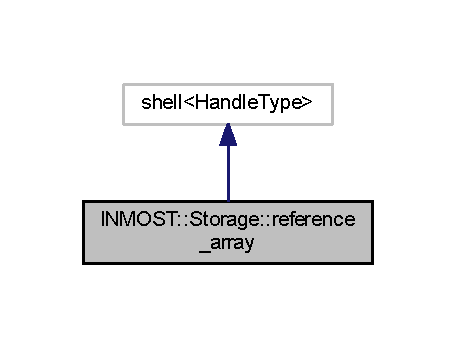
\includegraphics[width=219pt]{classINMOST_1_1Storage_1_1reference__array__inherit__graph}
\end{center}
\end{figure}


Collaboration diagram for I\-N\-M\-O\-S\-T\-:\-:Storage\-:\-:reference\-\_\-array\-:\nopagebreak
\begin{figure}[H]
\begin{center}
\leavevmode
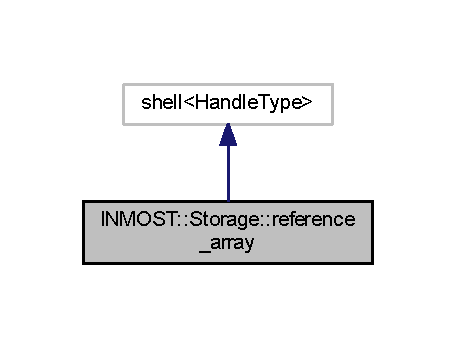
\includegraphics[width=219pt]{classINMOST_1_1Storage_1_1reference__array__coll__graph}
\end{center}
\end{figure}
\subsection*{Classes}
\begin{DoxyCompactItemize}
\item 
class \hyperlink{classINMOST_1_1Storage_1_1reference__array_1_1const__iterator}{const\-\_\-iterator}
\item 
class \hyperlink{classINMOST_1_1Storage_1_1reference__array_1_1const__reverse__iterator}{const\-\_\-reverse\-\_\-iterator}
\item 
class \hyperlink{classINMOST_1_1Storage_1_1reference__array_1_1iterator}{iterator}
\item 
class \hyperlink{classINMOST_1_1Storage_1_1reference__array_1_1reverse__iterator}{reverse\-\_\-iterator}
\end{DoxyCompactItemize}
\subsection*{Public Member Functions}
\begin{DoxyCompactItemize}
\item 
\hypertarget{classINMOST_1_1Storage_1_1reference__array_a4e01c7df6cdb5b59ae3212c384d9851b}{{\bfseries reference\-\_\-array} (\hyperlink{classINMOST_1_1Mesh}{Mesh} $\ast$m, inner\-\_\-reference\-\_\-array \&arr)}\label{classINMOST_1_1Storage_1_1reference__array_a4e01c7df6cdb5b59ae3212c384d9851b}

\item 
\hypertarget{classINMOST_1_1Storage_1_1reference__array_a2baea5e3b0592b79555788a468216623}{{\bfseries reference\-\_\-array} (\hyperlink{classINMOST_1_1Mesh}{Mesh} $\ast$m, \hyperlink{classINMOST_1_1Storage_a8674802045ec170a3c9d0e3281545b54}{reference} $\ast$arr, size\-\_\-type size)}\label{classINMOST_1_1Storage_1_1reference__array_a2baea5e3b0592b79555788a468216623}

\item 
\hypertarget{classINMOST_1_1Storage_1_1reference__array_a1e023416b73f1ff803b8dea5d2a9dcc0}{void {\bfseries push\-\_\-back} (const \hyperlink{classINMOST_1_1Storage}{Storage} \&elem)}\label{classINMOST_1_1Storage_1_1reference__array_a1e023416b73f1ff803b8dea5d2a9dcc0}

\item 
\hypertarget{classINMOST_1_1Storage_1_1reference__array_aff2da30cdc5284d11aea62b37964f34f}{void {\bfseries push\-\_\-back} (Handle\-Type h)}\label{classINMOST_1_1Storage_1_1reference__array_aff2da30cdc5284d11aea62b37964f34f}

\item 
\hypertarget{classINMOST_1_1Storage_1_1reference__array_a5ab5d6fab497a337926c16a46e5a58ee}{\hyperlink{classINMOST_1_1Element}{Element} {\bfseries operator\mbox{[}$\,$\mbox{]}} (size\-\_\-type n)}\label{classINMOST_1_1Storage_1_1reference__array_a5ab5d6fab497a337926c16a46e5a58ee}

\item 
\hypertarget{classINMOST_1_1Storage_1_1reference__array_aa39ff3355bc37bfab5e2ec7cca938aa6}{\hyperlink{classINMOST_1_1Element}{Element} {\bfseries operator\mbox{[}$\,$\mbox{]}} (size\-\_\-type n) const }\label{classINMOST_1_1Storage_1_1reference__array_aa39ff3355bc37bfab5e2ec7cca938aa6}

\item 
\hypertarget{classINMOST_1_1Storage_1_1reference__array_ab7b643e070fdfdf3a34eb83e0e41f1f4}{\hyperlink{classINMOST_1_1Storage_1_1reference__array_1_1iterator}{iterator} {\bfseries begin} ()}\label{classINMOST_1_1Storage_1_1reference__array_ab7b643e070fdfdf3a34eb83e0e41f1f4}

\item 
\hypertarget{classINMOST_1_1Storage_1_1reference__array_ac959eafca7a3d14dba4c753a66c7e262}{\hyperlink{classINMOST_1_1Storage_1_1reference__array_1_1const__iterator}{const\-\_\-iterator} {\bfseries begin} () const }\label{classINMOST_1_1Storage_1_1reference__array_ac959eafca7a3d14dba4c753a66c7e262}

\item 
\hypertarget{classINMOST_1_1Storage_1_1reference__array_abd39f6ff098a2c967b709ba93b1f143c}{\hyperlink{classINMOST_1_1Storage_1_1reference__array_1_1reverse__iterator}{reverse\-\_\-iterator} {\bfseries rbegin} ()}\label{classINMOST_1_1Storage_1_1reference__array_abd39f6ff098a2c967b709ba93b1f143c}

\item 
\hypertarget{classINMOST_1_1Storage_1_1reference__array_a9398aed4a995ef9e073af625b173f5cb}{\hyperlink{classINMOST_1_1Storage_1_1reference__array_1_1const__reverse__iterator}{const\-\_\-reverse\-\_\-iterator} {\bfseries rbegin} () const }\label{classINMOST_1_1Storage_1_1reference__array_a9398aed4a995ef9e073af625b173f5cb}

\item 
\hypertarget{classINMOST_1_1Storage_1_1reference__array_abbc83ae616e76a85735a13fc9db7e770}{\hyperlink{classINMOST_1_1Storage_1_1reference__array_1_1iterator}{iterator} {\bfseries end} ()}\label{classINMOST_1_1Storage_1_1reference__array_abbc83ae616e76a85735a13fc9db7e770}

\item 
\hypertarget{classINMOST_1_1Storage_1_1reference__array_a0a9db3b90f87fd6aae7f045dc5449b46}{\hyperlink{classINMOST_1_1Storage_1_1reference__array_1_1const__iterator}{const\-\_\-iterator} {\bfseries end} () const }\label{classINMOST_1_1Storage_1_1reference__array_a0a9db3b90f87fd6aae7f045dc5449b46}

\item 
\hypertarget{classINMOST_1_1Storage_1_1reference__array_a32765626cacfc8291fdf5edfa42f5f8c}{\hyperlink{classINMOST_1_1Storage_1_1reference__array_1_1reverse__iterator}{reverse\-\_\-iterator} {\bfseries rend} ()}\label{classINMOST_1_1Storage_1_1reference__array_a32765626cacfc8291fdf5edfa42f5f8c}

\item 
\hypertarget{classINMOST_1_1Storage_1_1reference__array_a7b2843949e49d1103cfbd0d466d4063c}{\hyperlink{classINMOST_1_1Storage_1_1reference__array_1_1const__reverse__iterator}{const\-\_\-reverse\-\_\-iterator} {\bfseries rend} () const }\label{classINMOST_1_1Storage_1_1reference__array_a7b2843949e49d1103cfbd0d466d4063c}

\item 
\hypertarget{classINMOST_1_1Storage_1_1reference__array_a01826ea5c06c905c319038a8017c704a}{void {\bfseries Set\-Mesh\-Link} (\hyperlink{classINMOST_1_1Mesh}{Mesh} $\ast$new\-\_\-m)}\label{classINMOST_1_1Storage_1_1reference__array_a01826ea5c06c905c319038a8017c704a}

\end{DoxyCompactItemize}


\subsection{Detailed Description}
\hyperlink{classINMOST_1_1Storage}{Storage} type for representing arrays of \hyperlink{classINMOST_1_1Element}{Element} references. 

The documentation for this class was generated from the following file\-:\begin{DoxyCompactItemize}
\item 
inmost\-\_\-mesh.\-h\end{DoxyCompactItemize}

\hypertarget{classINMOST_1_1Storage_1_1reference__array_1_1reverse__iterator}{\section{I\-N\-M\-O\-S\-T\-:\-:Storage\-:\-:reference\-\_\-array\-:\-:reverse\-\_\-iterator Class Reference}
\label{classINMOST_1_1Storage_1_1reference__array_1_1reverse__iterator}\index{I\-N\-M\-O\-S\-T\-::\-Storage\-::reference\-\_\-array\-::reverse\-\_\-iterator@{I\-N\-M\-O\-S\-T\-::\-Storage\-::reference\-\_\-array\-::reverse\-\_\-iterator}}
}


Inheritance diagram for I\-N\-M\-O\-S\-T\-:\-:Storage\-:\-:reference\-\_\-array\-:\-:reverse\-\_\-iterator\-:\nopagebreak
\begin{figure}[H]
\begin{center}
\leavevmode
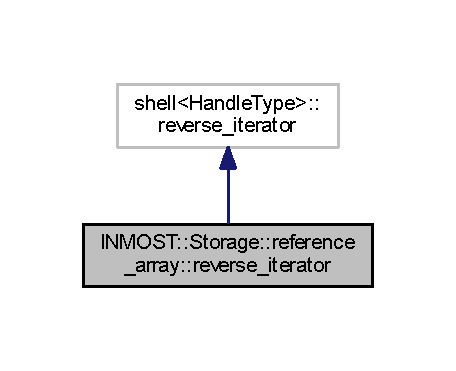
\includegraphics[width=219pt]{classINMOST_1_1Storage_1_1reference__array_1_1reverse__iterator__inherit__graph}
\end{center}
\end{figure}


Collaboration diagram for I\-N\-M\-O\-S\-T\-:\-:Storage\-:\-:reference\-\_\-array\-:\-:reverse\-\_\-iterator\-:\nopagebreak
\begin{figure}[H]
\begin{center}
\leavevmode
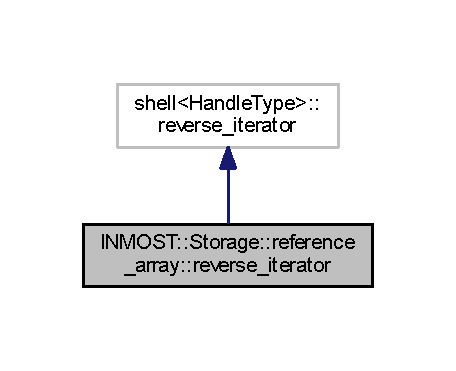
\includegraphics[width=219pt]{classINMOST_1_1Storage_1_1reference__array_1_1reverse__iterator__coll__graph}
\end{center}
\end{figure}
\subsection*{Public Member Functions}
\begin{DoxyCompactItemize}
\item 
\hypertarget{classINMOST_1_1Storage_1_1reference__array_1_1reverse__iterator_a2a8f7c0ad04bb4c642b9e16582076d64}{{\bfseries reverse\-\_\-iterator} (\hyperlink{classINMOST_1_1Mesh}{Mesh} $\ast$m, const shell$<$ Handle\-Type $>$\-::\hyperlink{classINMOST_1_1Storage_1_1reference__array_1_1reverse__iterator}{reverse\-\_\-iterator} \&other)}\label{classINMOST_1_1Storage_1_1reference__array_1_1reverse__iterator_a2a8f7c0ad04bb4c642b9e16582076d64}

\item 
\hypertarget{classINMOST_1_1Storage_1_1reference__array_1_1reverse__iterator_abe9465a93095e80e2247aad718b1bdd6}{{\bfseries reverse\-\_\-iterator} (const \hyperlink{classINMOST_1_1Storage_1_1reference__array_1_1reverse__iterator}{reverse\-\_\-iterator} \&other)}\label{classINMOST_1_1Storage_1_1reference__array_1_1reverse__iterator_abe9465a93095e80e2247aad718b1bdd6}

\item 
\hypertarget{classINMOST_1_1Storage_1_1reference__array_1_1reverse__iterator_ab91cad1582e0bb72352b9c437eed15d1}{\hyperlink{classINMOST_1_1Storage_1_1reference__array_1_1reverse__iterator}{reverse\-\_\-iterator} \& {\bfseries operator=} (\hyperlink{classINMOST_1_1Storage_1_1reference__array_1_1reverse__iterator}{reverse\-\_\-iterator} const \&other)}\label{classINMOST_1_1Storage_1_1reference__array_1_1reverse__iterator_ab91cad1582e0bb72352b9c437eed15d1}

\item 
\hypertarget{classINMOST_1_1Storage_1_1reference__array_1_1reverse__iterator_a59d86ffeb0a194b1be6535c881d9f772}{\hyperlink{classINMOST_1_1Storage_1_1reference__array_1_1reverse__iterator}{reverse\-\_\-iterator} \& {\bfseries operator++} ()}\label{classINMOST_1_1Storage_1_1reference__array_1_1reverse__iterator_a59d86ffeb0a194b1be6535c881d9f772}

\item 
\hypertarget{classINMOST_1_1Storage_1_1reference__array_1_1reverse__iterator_ac8021b73c7aa98d35b0cf0ba44752e78}{\hyperlink{classINMOST_1_1Storage_1_1reference__array_1_1reverse__iterator}{reverse\-\_\-iterator} {\bfseries operator++} (int)}\label{classINMOST_1_1Storage_1_1reference__array_1_1reverse__iterator_ac8021b73c7aa98d35b0cf0ba44752e78}

\item 
\hypertarget{classINMOST_1_1Storage_1_1reference__array_1_1reverse__iterator_a711c9e146000dfdaf604e6c8a2994988}{\hyperlink{classINMOST_1_1Storage_1_1reference__array_1_1reverse__iterator}{reverse\-\_\-iterator} \& {\bfseries operator-\/-\/} ()}\label{classINMOST_1_1Storage_1_1reference__array_1_1reverse__iterator_a711c9e146000dfdaf604e6c8a2994988}

\item 
\hypertarget{classINMOST_1_1Storage_1_1reference__array_1_1reverse__iterator_a15a67085cd14aed2ed15429f18b1fc8b}{\hyperlink{classINMOST_1_1Storage_1_1reference__array_1_1reverse__iterator}{reverse\-\_\-iterator} {\bfseries operator-\/-\/} (int)}\label{classINMOST_1_1Storage_1_1reference__array_1_1reverse__iterator_a15a67085cd14aed2ed15429f18b1fc8b}

\item 
\hypertarget{classINMOST_1_1Storage_1_1reference__array_1_1reverse__iterator_a6990d74c26cd22c2975872b693c1665c}{\hyperlink{classINMOST_1_1Element}{Element} {\bfseries operator-\/$>$} ()}\label{classINMOST_1_1Storage_1_1reference__array_1_1reverse__iterator_a6990d74c26cd22c2975872b693c1665c}

\end{DoxyCompactItemize}


The documentation for this class was generated from the following file\-:\begin{DoxyCompactItemize}
\item 
inmost\-\_\-mesh.\-h\end{DoxyCompactItemize}

\hypertarget{classINMOST_1_1ElementArray_1_1reverse__iterator}{\section{I\-N\-M\-O\-S\-T\-:\-:Element\-Array$<$ Storage\-Type $>$\-:\-:reverse\-\_\-iterator Class Reference}
\label{classINMOST_1_1ElementArray_1_1reverse__iterator}\index{I\-N\-M\-O\-S\-T\-::\-Element\-Array$<$ Storage\-Type $>$\-::reverse\-\_\-iterator@{I\-N\-M\-O\-S\-T\-::\-Element\-Array$<$ Storage\-Type $>$\-::reverse\-\_\-iterator}}
}


Inheritance diagram for I\-N\-M\-O\-S\-T\-:\-:Element\-Array$<$ Storage\-Type $>$\-:\-:reverse\-\_\-iterator\-:\nopagebreak
\begin{figure}[H]
\begin{center}
\leavevmode
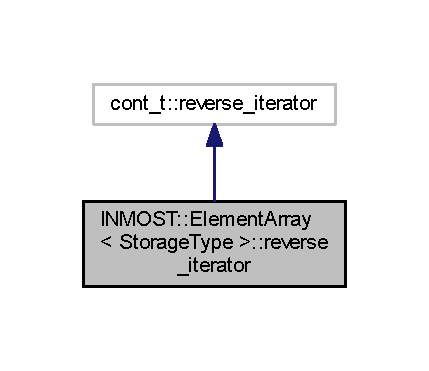
\includegraphics[width=206pt]{classINMOST_1_1ElementArray_1_1reverse__iterator__inherit__graph}
\end{center}
\end{figure}


Collaboration diagram for I\-N\-M\-O\-S\-T\-:\-:Element\-Array$<$ Storage\-Type $>$\-:\-:reverse\-\_\-iterator\-:\nopagebreak
\begin{figure}[H]
\begin{center}
\leavevmode
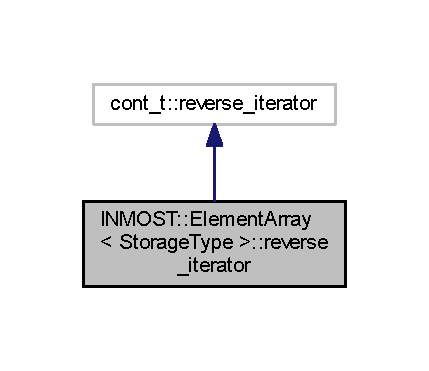
\includegraphics[width=206pt]{classINMOST_1_1ElementArray_1_1reverse__iterator__coll__graph}
\end{center}
\end{figure}
\subsection*{Public Member Functions}
\begin{DoxyCompactItemize}
\item 
\hypertarget{classINMOST_1_1ElementArray_1_1reverse__iterator_a31626bef2bdce5c06744ef82c215d815}{{\bfseries reverse\-\_\-iterator} (\hyperlink{classINMOST_1_1Mesh}{Mesh} $\ast$m, const cont\-\_\-t\-::reverse\-\_\-iterator \&other)}\label{classINMOST_1_1ElementArray_1_1reverse__iterator_a31626bef2bdce5c06744ef82c215d815}

\item 
\hypertarget{classINMOST_1_1ElementArray_1_1reverse__iterator_a35aeb6a3511335494e5cec02e7dfd2dd}{{\bfseries reverse\-\_\-iterator} (const \hyperlink{classINMOST_1_1ElementArray_1_1reverse__iterator}{reverse\-\_\-iterator} \&other)}\label{classINMOST_1_1ElementArray_1_1reverse__iterator_a35aeb6a3511335494e5cec02e7dfd2dd}

\item 
\hypertarget{classINMOST_1_1ElementArray_1_1reverse__iterator_aa7141990b0eb273db9b93f47a1238acb}{\hyperlink{classINMOST_1_1ElementArray_1_1reverse__iterator}{reverse\-\_\-iterator} \& {\bfseries operator++} ()}\label{classINMOST_1_1ElementArray_1_1reverse__iterator_aa7141990b0eb273db9b93f47a1238acb}

\item 
\hypertarget{classINMOST_1_1ElementArray_1_1reverse__iterator_addc4d8af50494b40947ec19ff4259bc3}{\hyperlink{classINMOST_1_1ElementArray_1_1reverse__iterator}{reverse\-\_\-iterator} {\bfseries operator++} (int)}\label{classINMOST_1_1ElementArray_1_1reverse__iterator_addc4d8af50494b40947ec19ff4259bc3}

\item 
\hypertarget{classINMOST_1_1ElementArray_1_1reverse__iterator_acd1a26fff5ef7b466cc9357e77207cb5}{\hyperlink{classINMOST_1_1ElementArray_1_1reverse__iterator}{reverse\-\_\-iterator} \& {\bfseries operator-\/-\/} ()}\label{classINMOST_1_1ElementArray_1_1reverse__iterator_acd1a26fff5ef7b466cc9357e77207cb5}

\item 
\hypertarget{classINMOST_1_1ElementArray_1_1reverse__iterator_ac2f1741086eeedb85d9b2d75e0b2a65b}{\hyperlink{classINMOST_1_1ElementArray_1_1reverse__iterator}{reverse\-\_\-iterator} {\bfseries operator-\/-\/} (int)}\label{classINMOST_1_1ElementArray_1_1reverse__iterator_ac2f1741086eeedb85d9b2d75e0b2a65b}

\item 
\hypertarget{classINMOST_1_1ElementArray_1_1reverse__iterator_ae984218ea8ae50771cffd51b4100641d}{\hyperlink{classINMOST_1_1ElementArray_1_1reverse__iterator}{reverse\-\_\-iterator} \& {\bfseries operator=} (\hyperlink{classINMOST_1_1ElementArray_1_1reverse__iterator}{reverse\-\_\-iterator} const \&other)}\label{classINMOST_1_1ElementArray_1_1reverse__iterator_ae984218ea8ae50771cffd51b4100641d}

\item 
\hypertarget{classINMOST_1_1ElementArray_1_1reverse__iterator_a4aac2a4476ad6d4d07f6506ff765c899}{Handle\-Type \& {\bfseries operator$\ast$} ()}\label{classINMOST_1_1ElementArray_1_1reverse__iterator_a4aac2a4476ad6d4d07f6506ff765c899}

\item 
\hypertarget{classINMOST_1_1ElementArray_1_1reverse__iterator_aec20290a8c598c305deebc5c1c7652a4}{Storage\-Type {\bfseries operator-\/$>$} ()}\label{classINMOST_1_1ElementArray_1_1reverse__iterator_aec20290a8c598c305deebc5c1c7652a4}

\end{DoxyCompactItemize}


The documentation for this class was generated from the following file\-:\begin{DoxyCompactItemize}
\item 
inmost\-\_\-mesh.\-h\end{DoxyCompactItemize}

\hypertarget{classINMOST_1_1Solver_1_1Row}{\section{I\-N\-M\-O\-S\-T\-:\-:Solver\-:\-:Row Class Reference}
\label{classINMOST_1_1Solver_1_1Row}\index{I\-N\-M\-O\-S\-T\-::\-Solver\-::\-Row@{I\-N\-M\-O\-S\-T\-::\-Solver\-::\-Row}}
}


Class to store the sparse matrix row.  




{\ttfamily \#include $<$inmost\-\_\-solver.\-h$>$}

\subsection*{Classes}
\begin{DoxyCompactItemize}
\item 
struct \hyperlink{structINMOST_1_1Solver_1_1Row_1_1entry__s}{entry\-\_\-s}
\begin{DoxyCompactList}\small\item\em Entry of the sparse matrix row. \end{DoxyCompactList}\end{DoxyCompactItemize}
\subsection*{Public Types}
\begin{DoxyCompactItemize}
\item 
\hypertarget{classINMOST_1_1Solver_1_1Row_a83f9b826189f21abd7ad395608901825}{typedef struct \\*
\hyperlink{structINMOST_1_1Solver_1_1Row_1_1entry__s}{I\-N\-M\-O\-S\-T\-::\-Solver\-::\-Row\-::entry\-\_\-s} \hyperlink{classINMOST_1_1Solver_1_1Row_a83f9b826189f21abd7ad395608901825}{entry}}\label{classINMOST_1_1Solver_1_1Row_a83f9b826189f21abd7ad395608901825}

\begin{DoxyCompactList}\small\item\em Entry of the sparse matrix row. \end{DoxyCompactList}\item 
\hypertarget{classINMOST_1_1Solver_1_1Row_afbcd3de717631f8d5d2dd53ebaf3855b}{typedef dynarray$<$ \hyperlink{classINMOST_1_1Solver_1_1Row_a83f9b826189f21abd7ad395608901825}{entry}, 16 $>$ {\bfseries Entries}}\label{classINMOST_1_1Solver_1_1Row_afbcd3de717631f8d5d2dd53ebaf3855b}

\item 
\hypertarget{classINMOST_1_1Solver_1_1Row_ab8acd9e8e471bcc8e0ef5acf4974e3e3}{typedef Entries\-::iterator {\bfseries iterator}}\label{classINMOST_1_1Solver_1_1Row_ab8acd9e8e471bcc8e0ef5acf4974e3e3}

\item 
\hypertarget{classINMOST_1_1Solver_1_1Row_a20fda02b31081d59482d9bbe1d2219be}{typedef Entries\-::const\-\_\-iterator {\bfseries const\-\_\-iterator}}\label{classINMOST_1_1Solver_1_1Row_a20fda02b31081d59482d9bbe1d2219be}

\item 
\hypertarget{classINMOST_1_1Solver_1_1Row_a5b9530cb6fce446eea45ce9128b8feef}{typedef Entries\-::reverse\-\_\-iterator {\bfseries reverse\-\_\-iterator}}\label{classINMOST_1_1Solver_1_1Row_a5b9530cb6fce446eea45ce9128b8feef}

\item 
\hypertarget{classINMOST_1_1Solver_1_1Row_a8917a1291254817a0ed93c9b62c53f58}{typedef \\*
Entries\-::const\-\_\-reverse\-\_\-iterator {\bfseries const\-\_\-reverse\-\_\-iterator}}\label{classINMOST_1_1Solver_1_1Row_a8917a1291254817a0ed93c9b62c53f58}

\end{DoxyCompactItemize}
\subsection*{Public Member Functions}
\begin{DoxyCompactItemize}
\item 
\hypertarget{classINMOST_1_1Solver_1_1Row_a0118f755b9f625a86daec89fb0fd3b10}{void {\bfseries Report} ()}\label{classINMOST_1_1Solver_1_1Row_a0118f755b9f625a86daec89fb0fd3b10}

\item 
\hypertarget{classINMOST_1_1Solver_1_1Row_a636ac5a6d862b93a81706022ba3656bb}{void {\bfseries Set\-Marker} ()}\label{classINMOST_1_1Solver_1_1Row_a636ac5a6d862b93a81706022ba3656bb}

\item 
\hypertarget{classINMOST_1_1Solver_1_1Row_a21da67468799355d250d8b9a1203303a}{void {\bfseries Rem\-Marker} ()}\label{classINMOST_1_1Solver_1_1Row_a21da67468799355d250d8b9a1203303a}

\item 
\hypertarget{classINMOST_1_1Solver_1_1Row_affe6afd6d1360741bbda3da9ece864ca}{bool {\bfseries Get\-Marker} ()}\label{classINMOST_1_1Solver_1_1Row_affe6afd6d1360741bbda3da9ece864ca}

\item 
\hypertarget{classINMOST_1_1Solver_1_1Row_aab8578ccd5366204ee4db2bd0350dbf4}{{\bfseries Row} (const \hyperlink{classINMOST_1_1Solver_1_1Row}{Row} \&other)}\label{classINMOST_1_1Solver_1_1Row_aab8578ccd5366204ee4db2bd0350dbf4}

\item 
\hypertarget{classINMOST_1_1Solver_1_1Row_ada200daf944fd240ec23d41c8dd9b0c1}{{\bfseries Row} (\hyperlink{classINMOST_1_1Solver_1_1Row_a83f9b826189f21abd7ad395608901825}{entry} $\ast$pbegin, \hyperlink{classINMOST_1_1Solver_1_1Row_a83f9b826189f21abd7ad395608901825}{entry} $\ast$pend)}\label{classINMOST_1_1Solver_1_1Row_ada200daf944fd240ec23d41c8dd9b0c1}

\item 
\hypertarget{classINMOST_1_1Solver_1_1Row_aefcfbbcf45bb6ac91990c3814d87ef6d}{void {\bfseries Lock} ()}\label{classINMOST_1_1Solver_1_1Row_aefcfbbcf45bb6ac91990c3814d87ef6d}

\item 
\hypertarget{classINMOST_1_1Solver_1_1Row_ac2945647b3ab8a2e6fcbcf148175056d}{void {\bfseries Unlock} ()}\label{classINMOST_1_1Solver_1_1Row_ac2945647b3ab8a2e6fcbcf148175056d}

\item 
\hypertarget{classINMOST_1_1Solver_1_1Row_a88fbacc12cd00bc3e9508e4180cb3d72}{\hyperlink{classINMOST_1_1Solver_1_1Row}{Row} \& {\bfseries operator=} (\hyperlink{classINMOST_1_1Solver_1_1Row}{Row} const \&other)}\label{classINMOST_1_1Solver_1_1Row_a88fbacc12cd00bc3e9508e4180cb3d72}

\item 
\hypertarget{classINMOST_1_1Solver_1_1Row_afaef4cd8aebf4d290f4503de194f7910}{I\-N\-M\-O\-S\-T\-\_\-\-D\-A\-T\-A\-\_\-\-R\-E\-A\-L\-\_\-\-T\-Y\-P\-E \& \hyperlink{classINMOST_1_1Solver_1_1Row_afaef4cd8aebf4d290f4503de194f7910}{operator\mbox{[}$\,$\mbox{]}} (I\-N\-M\-O\-S\-T\-\_\-\-D\-A\-T\-A\-\_\-\-E\-N\-U\-M\-\_\-\-T\-Y\-P\-E i)}\label{classINMOST_1_1Solver_1_1Row_afaef4cd8aebf4d290f4503de194f7910}

\begin{DoxyCompactList}\small\item\em The operator \mbox{[}\mbox{]} used to fill the sparse matrix row, but not to access individual elements of the row. \end{DoxyCompactList}\item 
\hypertarget{classINMOST_1_1Solver_1_1Row_ae65332e42ee2fdf2755d6200a7750eaf}{I\-N\-M\-O\-S\-T\-\_\-\-D\-A\-T\-A\-\_\-\-R\-E\-A\-L\-\_\-\-T\-Y\-P\-E \hyperlink{classINMOST_1_1Solver_1_1Row_ae65332e42ee2fdf2755d6200a7750eaf}{operator\mbox{[}$\,$\mbox{]}} (I\-N\-M\-O\-S\-T\-\_\-\-D\-A\-T\-A\-\_\-\-E\-N\-U\-M\-\_\-\-T\-Y\-P\-E i) const }\label{classINMOST_1_1Solver_1_1Row_ae65332e42ee2fdf2755d6200a7750eaf}

\begin{DoxyCompactList}\small\item\em The operator \mbox{[}\mbox{]} used to access individual elements of the row. \end{DoxyCompactList}\item 
\hypertarget{classINMOST_1_1Solver_1_1Row_ac86e436d943e530c3f0dd3d9f22b8fdf}{void \hyperlink{classINMOST_1_1Solver_1_1Row_ac86e436d943e530c3f0dd3d9f22b8fdf}{Clear} ()}\label{classINMOST_1_1Solver_1_1Row_ac86e436d943e530c3f0dd3d9f22b8fdf}

\begin{DoxyCompactList}\small\item\em Clear all data of the current row. \end{DoxyCompactList}\item 
\hypertarget{classINMOST_1_1Solver_1_1Row_aab38e0f7e84952a0bb62d23338445580}{void {\bfseries Swap} (\hyperlink{classINMOST_1_1Solver_1_1Row}{Solver\-::\-Row} \&other)}\label{classINMOST_1_1Solver_1_1Row_aab38e0f7e84952a0bb62d23338445580}

\item 
\hypertarget{classINMOST_1_1Solver_1_1Row_aa1e5f7bccac23fee20de403374b5cc65}{I\-N\-M\-O\-S\-T\-\_\-\-D\-A\-T\-A\-\_\-\-E\-N\-U\-M\-\_\-\-T\-Y\-P\-E \hyperlink{classINMOST_1_1Solver_1_1Row_aa1e5f7bccac23fee20de403374b5cc65}{Size} () const }\label{classINMOST_1_1Solver_1_1Row_aa1e5f7bccac23fee20de403374b5cc65}

\begin{DoxyCompactList}\small\item\em The size of the sparse row, i.\-e. the total number of nonzero elements. \end{DoxyCompactList}\item 
\hypertarget{classINMOST_1_1Solver_1_1Row_aeeaec59f6d6f5e8eb96cd2f4dfbf1f45}{I\-N\-M\-O\-S\-T\-\_\-\-D\-A\-T\-A\-\_\-\-E\-N\-U\-M\-\_\-\-T\-Y\-P\-E \& {\bfseries Get\-Index} (I\-N\-M\-O\-S\-T\-\_\-\-D\-A\-T\-A\-\_\-\-E\-N\-U\-M\-\_\-\-T\-Y\-P\-E k)}\label{classINMOST_1_1Solver_1_1Row_aeeaec59f6d6f5e8eb96cd2f4dfbf1f45}

\item 
\hypertarget{classINMOST_1_1Solver_1_1Row_aa55f0df7ce1445b8a3141c45b78839c1}{I\-N\-M\-O\-S\-T\-\_\-\-D\-A\-T\-A\-\_\-\-R\-E\-A\-L\-\_\-\-T\-Y\-P\-E \& {\bfseries Get\-Value} (I\-N\-M\-O\-S\-T\-\_\-\-D\-A\-T\-A\-\_\-\-E\-N\-U\-M\-\_\-\-T\-Y\-P\-E k)}\label{classINMOST_1_1Solver_1_1Row_aa55f0df7ce1445b8a3141c45b78839c1}

\item 
\hypertarget{classINMOST_1_1Solver_1_1Row_aadebc4bfba05b2f5cb274dc904c5ca2a}{I\-N\-M\-O\-S\-T\-\_\-\-D\-A\-T\-A\-\_\-\-E\-N\-U\-M\-\_\-\-T\-Y\-P\-E {\bfseries Get\-Index} (I\-N\-M\-O\-S\-T\-\_\-\-D\-A\-T\-A\-\_\-\-E\-N\-U\-M\-\_\-\-T\-Y\-P\-E k) const }\label{classINMOST_1_1Solver_1_1Row_aadebc4bfba05b2f5cb274dc904c5ca2a}

\item 
\hypertarget{classINMOST_1_1Solver_1_1Row_a8078b3435a0d2fef8ee285ed045a6cd2}{I\-N\-M\-O\-S\-T\-\_\-\-D\-A\-T\-A\-\_\-\-R\-E\-A\-L\-\_\-\-T\-Y\-P\-E {\bfseries Get\-Value} (I\-N\-M\-O\-S\-T\-\_\-\-D\-A\-T\-A\-\_\-\-E\-N\-U\-M\-\_\-\-T\-Y\-P\-E k) const }\label{classINMOST_1_1Solver_1_1Row_a8078b3435a0d2fef8ee285ed045a6cd2}

\item 
\hypertarget{classINMOST_1_1Solver_1_1Row_a04f7f359a9ec0a3ae0c4b74586e25398}{iterator {\bfseries Begin} ()}\label{classINMOST_1_1Solver_1_1Row_a04f7f359a9ec0a3ae0c4b74586e25398}

\item 
\hypertarget{classINMOST_1_1Solver_1_1Row_ace5b0538e549c621956412c3f6edce16}{iterator {\bfseries End} ()}\label{classINMOST_1_1Solver_1_1Row_ace5b0538e549c621956412c3f6edce16}

\item 
\hypertarget{classINMOST_1_1Solver_1_1Row_a8944846feb4a1d33df5ac39d0d84929f}{const\-\_\-iterator {\bfseries Begin} () const }\label{classINMOST_1_1Solver_1_1Row_a8944846feb4a1d33df5ac39d0d84929f}

\item 
\hypertarget{classINMOST_1_1Solver_1_1Row_a8ad80117dea23ed625e13d88fff017c0}{const\-\_\-iterator {\bfseries End} () const }\label{classINMOST_1_1Solver_1_1Row_a8ad80117dea23ed625e13d88fff017c0}

\item 
\hypertarget{classINMOST_1_1Solver_1_1Row_a144833591962eda366d902a1bbc5859c}{reverse\-\_\-iterator {\bfseries r\-Begin} ()}\label{classINMOST_1_1Solver_1_1Row_a144833591962eda366d902a1bbc5859c}

\item 
\hypertarget{classINMOST_1_1Solver_1_1Row_ae6029686b9d4203f940fbc25105abda2}{reverse\-\_\-iterator {\bfseries r\-End} ()}\label{classINMOST_1_1Solver_1_1Row_ae6029686b9d4203f940fbc25105abda2}

\item 
\hypertarget{classINMOST_1_1Solver_1_1Row_a5d3967eb389061b8efed504154814f36}{const\-\_\-reverse\-\_\-iterator {\bfseries r\-Begin} () const }\label{classINMOST_1_1Solver_1_1Row_a5d3967eb389061b8efed504154814f36}

\item 
\hypertarget{classINMOST_1_1Solver_1_1Row_a10a4f2916edf251ee04cea7c1f6502b7}{const\-\_\-reverse\-\_\-iterator {\bfseries r\-End} () const }\label{classINMOST_1_1Solver_1_1Row_a10a4f2916edf251ee04cea7c1f6502b7}

\item 
\hypertarget{classINMOST_1_1Solver_1_1Row_ac9cbd7928544cfffe5e8ad8ccea269cb}{I\-N\-M\-O\-S\-T\-\_\-\-D\-A\-T\-A\-\_\-\-R\-E\-A\-L\-\_\-\-T\-Y\-P\-E \hyperlink{classINMOST_1_1Solver_1_1Row_ac9cbd7928544cfffe5e8ad8ccea269cb}{Row\-Vec} (\hyperlink{classINMOST_1_1Solver_1_1Vector}{Vector} \&x) const }\label{classINMOST_1_1Solver_1_1Row_ac9cbd7928544cfffe5e8ad8ccea269cb}

\begin{DoxyCompactList}\small\item\em Return the scalar product of the current sparse row by a dense \hyperlink{classINMOST_1_1Solver_1_1Vector}{Vector}. \end{DoxyCompactList}\item 
\hypertarget{classINMOST_1_1Solver_1_1Row_a67f9cbe973e71fa8b9ba1dc92256b75a}{void {\bfseries Move\-Row} (\hyperlink{classINMOST_1_1Solver_1_1Row}{Row} \&new\-\_\-pos)}\label{classINMOST_1_1Solver_1_1Row_a67f9cbe973e71fa8b9ba1dc92256b75a}

\item 
\hypertarget{classINMOST_1_1Solver_1_1Row_af7022d7b2c223927e07b22f43584c93b}{void \hyperlink{classINMOST_1_1Solver_1_1Row_af7022d7b2c223927e07b22f43584c93b}{Zero} ()}\label{classINMOST_1_1Solver_1_1Row_af7022d7b2c223927e07b22f43584c93b}

\begin{DoxyCompactList}\small\item\em Set the vector entries by zeroes. \end{DoxyCompactList}\item 
void \hyperlink{classINMOST_1_1Solver_1_1Row_af5a53ab2f8e8febc9ce3196ff054cb01}{Push} (I\-N\-M\-O\-S\-T\-\_\-\-D\-A\-T\-A\-\_\-\-E\-N\-U\-M\-\_\-\-T\-Y\-P\-E ind, I\-N\-M\-O\-S\-T\-\_\-\-D\-A\-T\-A\-\_\-\-R\-E\-A\-L\-\_\-\-T\-Y\-P\-E val)
\begin{DoxyCompactList}\small\item\em Push specified element into sparse row. \end{DoxyCompactList}\item 
void \hyperlink{classINMOST_1_1Solver_1_1Row_a5465388e8b93e0f2fe32fe62e29640ad}{Resize} (I\-N\-M\-O\-S\-T\-\_\-\-D\-A\-T\-A\-\_\-\-E\-N\-U\-M\-\_\-\-T\-Y\-P\-E size)
\begin{DoxyCompactList}\small\item\em Resize row to specified size. \end{DoxyCompactList}\end{DoxyCompactItemize}
\subsection*{Static Public Member Functions}
\begin{DoxyCompactItemize}
\item 
\hypertarget{classINMOST_1_1Solver_1_1Row_a709889bdf720d73e7aa874b5b6a0d231}{static \-\_\-\-\_\-\-I\-N\-L\-I\-N\-E \hyperlink{classINMOST_1_1Solver_1_1Row_a83f9b826189f21abd7ad395608901825}{entry} {\bfseries make\-\_\-entry} (I\-N\-M\-O\-S\-T\-\_\-\-D\-A\-T\-A\-\_\-\-E\-N\-U\-M\-\_\-\-T\-Y\-P\-E ind, I\-N\-M\-O\-S\-T\-\_\-\-D\-A\-T\-A\-\_\-\-R\-E\-A\-L\-\_\-\-T\-Y\-P\-E val)}\label{classINMOST_1_1Solver_1_1Row_a709889bdf720d73e7aa874b5b6a0d231}

\end{DoxyCompactItemize}
\subsection*{Public Attributes}
\begin{DoxyCompactItemize}
\item 
\hypertarget{classINMOST_1_1Solver_1_1Row_a417f7f35421de05227023d03a1c9c095}{bool {\bfseries modified\-\_\-pattern}}\label{classINMOST_1_1Solver_1_1Row_a417f7f35421de05227023d03a1c9c095}

\end{DoxyCompactItemize}


\subsection{Detailed Description}
Class to store the sparse matrix row. 

\subsection{Member Function Documentation}
\hypertarget{classINMOST_1_1Solver_1_1Row_af5a53ab2f8e8febc9ce3196ff054cb01}{\index{I\-N\-M\-O\-S\-T\-::\-Solver\-::\-Row@{I\-N\-M\-O\-S\-T\-::\-Solver\-::\-Row}!Push@{Push}}
\index{Push@{Push}!INMOST::Solver::Row@{I\-N\-M\-O\-S\-T\-::\-Solver\-::\-Row}}
\subsubsection[{Push}]{\setlength{\rightskip}{0pt plus 5cm}void I\-N\-M\-O\-S\-T\-::\-Solver\-::\-Row\-::\-Push (
\begin{DoxyParamCaption}
\item[{I\-N\-M\-O\-S\-T\-\_\-\-D\-A\-T\-A\-\_\-\-E\-N\-U\-M\-\_\-\-T\-Y\-P\-E}]{ind, }
\item[{I\-N\-M\-O\-S\-T\-\_\-\-D\-A\-T\-A\-\_\-\-R\-E\-A\-L\-\_\-\-T\-Y\-P\-E}]{val}
\end{DoxyParamCaption}
)\hspace{0.3cm}{\ttfamily [inline]}}}\label{classINMOST_1_1Solver_1_1Row_af5a53ab2f8e8febc9ce3196ff054cb01}


Push specified element into sparse row. 

This function should be used only if the index is not repeated in the row. \hypertarget{classINMOST_1_1Solver_1_1Row_a5465388e8b93e0f2fe32fe62e29640ad}{\index{I\-N\-M\-O\-S\-T\-::\-Solver\-::\-Row@{I\-N\-M\-O\-S\-T\-::\-Solver\-::\-Row}!Resize@{Resize}}
\index{Resize@{Resize}!INMOST::Solver::Row@{I\-N\-M\-O\-S\-T\-::\-Solver\-::\-Row}}
\subsubsection[{Resize}]{\setlength{\rightskip}{0pt plus 5cm}void I\-N\-M\-O\-S\-T\-::\-Solver\-::\-Row\-::\-Resize (
\begin{DoxyParamCaption}
\item[{I\-N\-M\-O\-S\-T\-\_\-\-D\-A\-T\-A\-\_\-\-E\-N\-U\-M\-\_\-\-T\-Y\-P\-E}]{size}
\end{DoxyParamCaption}
)\hspace{0.3cm}{\ttfamily [inline]}}}\label{classINMOST_1_1Solver_1_1Row_a5465388e8b93e0f2fe32fe62e29640ad}


Resize row to specified size. 

It is intended to be used together with non-\/const Row\-::\-Get\-Index and Row\-::\-Get\-Value that allow for the modification of individual entries. 
\begin{DoxyParams}{Parameters}
{\em size} & New size of the row. \\
\hline
\end{DoxyParams}


The documentation for this class was generated from the following file\-:\begin{DoxyCompactItemize}
\item 
inmost\-\_\-solver.\-h\end{DoxyCompactItemize}

\hypertarget{classINMOST_1_1Solver}{\section{I\-N\-M\-O\-S\-T\-:\-:Solver Class Reference}
\label{classINMOST_1_1Solver}\index{I\-N\-M\-O\-S\-T\-::\-Solver@{I\-N\-M\-O\-S\-T\-::\-Solver}}
}


Main class to set and solve linear system.  




{\ttfamily \#include $<$inmost\-\_\-solver.\-h$>$}

\subsection*{Classes}
\begin{DoxyCompactItemize}
\item 
class \hyperlink{classINMOST_1_1Solver_1_1Matrix}{Matrix}
\begin{DoxyCompactList}\small\item\em Class to store the distributed sparse matrix by compressed rows. \end{DoxyCompactList}\item 
class \hyperlink{classINMOST_1_1Solver_1_1OrderInfo}{Order\-Info}
\begin{DoxyCompactList}\small\item\em Base class for low level operations with objects of \hyperlink{classINMOST_1_1Solver}{Solver} class. \end{DoxyCompactList}\item 
class \hyperlink{classINMOST_1_1Solver_1_1Row}{Row}
\begin{DoxyCompactList}\small\item\em Class to store the sparse matrix row. \end{DoxyCompactList}\item 
class \hyperlink{classINMOST_1_1Solver_1_1Vector}{Vector}
\begin{DoxyCompactList}\small\item\em Distributed vector class. \end{DoxyCompactList}\end{DoxyCompactItemize}
\subsection*{Public Types}
\begin{DoxyCompactItemize}
\item 
enum \hyperlink{classINMOST_1_1Solver_ad21ba852fdfe10116b40aac266c0309b}{Type} \{ \\*
\hyperlink{classINMOST_1_1Solver_ad21ba852fdfe10116b40aac266c0309baf63e1ad7b5ae2acdd4ae0a0f5638721b}{I\-N\-N\-E\-R\-\_\-\-I\-L\-U2}, 
\hyperlink{classINMOST_1_1Solver_ad21ba852fdfe10116b40aac266c0309badee0e7d52b15257e3da8f03c386ff4fb}{I\-N\-N\-E\-R\-\_\-\-M\-L\-I\-L\-U\-C}, 
\hyperlink{classINMOST_1_1Solver_ad21ba852fdfe10116b40aac266c0309bad44d0870437e0d0feb62902415ab70c6}{Trilinos\-\_\-\-Aztec}, 
\hyperlink{classINMOST_1_1Solver_ad21ba852fdfe10116b40aac266c0309bab0bdd8110a229561e0beafaa87ec39ba}{Trilinos\-\_\-\-Belos}, 
\\*
\hyperlink{classINMOST_1_1Solver_ad21ba852fdfe10116b40aac266c0309ba3dd85459b7a587d7f73c5c6b8f48e442}{Trilinos\-\_\-\-M\-L}, 
\hyperlink{classINMOST_1_1Solver_ad21ba852fdfe10116b40aac266c0309ba8045d698296fd9b11ad749400be138ad}{Trilinos\-\_\-\-Ifpack}, 
\hyperlink{classINMOST_1_1Solver_ad21ba852fdfe10116b40aac266c0309ba4836875066e4576bfa281cea50739107}{P\-E\-T\-Sc}, 
\hyperlink{classINMOST_1_1Solver_ad21ba852fdfe10116b40aac266c0309ba5392887dbb97c84546fc3eeb010729c9}{A\-N\-I}
 \}
\begin{DoxyCompactList}\small\item\em Type of the \hyperlink{classINMOST_1_1Solver}{Solver} can be currently used in this version of I\-N\-M\-O\-S\-T. \end{DoxyCompactList}\end{DoxyCompactItemize}
\subsection*{Public Member Functions}
\begin{DoxyCompactItemize}
\item 
void \hyperlink{classINMOST_1_1Solver_a099f1bc2e5f530a30ff37f5fc3033d8a}{Set\-Parameter\-Enum} (std\-::string name, I\-N\-M\-O\-S\-T\-\_\-\-D\-A\-T\-A\-\_\-\-E\-N\-U\-M\-\_\-\-T\-Y\-P\-E value)
\begin{DoxyCompactList}\small\item\em Set the solver parameter of the integer type. \end{DoxyCompactList}\item 
void \hyperlink{classINMOST_1_1Solver_a7997f1ad3cce898632e582de27f08a42}{Set\-Parameter\-Real} (std\-::string name, I\-N\-M\-O\-S\-T\-\_\-\-D\-A\-T\-A\-\_\-\-R\-E\-A\-L\-\_\-\-T\-Y\-P\-E value)
\begin{DoxyCompactList}\small\item\em Set the solver parameter of the real type. \end{DoxyCompactList}\item 
\hypertarget{classINMOST_1_1Solver_a19a57bde95128504e8c9cecde896ae53}{std\-::string \hyperlink{classINMOST_1_1Solver_a19a57bde95128504e8c9cecde896ae53}{Get\-Name} ()}\label{classINMOST_1_1Solver_a19a57bde95128504e8c9cecde896ae53}

\begin{DoxyCompactList}\small\item\em Get the used defined name of the \hyperlink{classINMOST_1_1Solver}{Solver}. \end{DoxyCompactList}\item 
\hypertarget{classINMOST_1_1Solver_a76ba3fc72df7ccf55bab47251265c576}{\hyperlink{classINMOST_1_1Solver_ad21ba852fdfe10116b40aac266c0309b}{Type} \hyperlink{classINMOST_1_1Solver_a76ba3fc72df7ccf55bab47251265c576}{Get\-Package} () const }\label{classINMOST_1_1Solver_a76ba3fc72df7ccf55bab47251265c576}

\begin{DoxyCompactList}\small\item\em Get the package Type. \end{DoxyCompactList}\item 
I\-N\-M\-O\-S\-T\-\_\-\-D\-A\-T\-A\-\_\-\-E\-N\-U\-M\-\_\-\-T\-Y\-P\-E \hyperlink{classINMOST_1_1Solver_ad943889a4b31789185eee09af14a5d45}{Iterations} ()
\begin{DoxyCompactList}\small\item\em Return the number of iterations performed by the last solution. \end{DoxyCompactList}\item 
I\-N\-M\-O\-S\-T\-\_\-\-D\-A\-T\-A\-\_\-\-R\-E\-A\-L\-\_\-\-T\-Y\-P\-E \hyperlink{classINMOST_1_1Solver_ad10f8b22ba2d3c4ecbb4c22abfc62266}{Residual} ()
\begin{DoxyCompactList}\small\item\em Return the final residual achieved by the last solution. \end{DoxyCompactList}\item 
void \hyperlink{classINMOST_1_1Solver_a8e70ae0ef4eaa220d1db45089b4df1ff}{Set\-Matrix} (\hyperlink{classINMOST_1_1Solver_1_1Matrix}{Matrix} \&A, bool Old\-Preconditioner=false)
\begin{DoxyCompactList}\small\item\em Set the matrix and construct the preconditioner. \end{DoxyCompactList}\item 
bool \hyperlink{classINMOST_1_1Solver_ab31891d2c65c0ac93c06b91222b5cbfd}{Solve} (\hyperlink{classINMOST_1_1Solver_1_1Vector}{Vector} \&R\-H\-S, \hyperlink{classINMOST_1_1Solver_1_1Vector}{Vector} \&S\-O\-L)
\begin{DoxyCompactList}\small\item\em \hyperlink{classINMOST_1_1Solver}{Solver} the linear system\-: A$\ast$x = b. \end{DoxyCompactList}\item 
std\-::string \hyperlink{classINMOST_1_1Solver_afc0502769ba027228e7bda966498ebb5}{Get\-Reason} ()
\begin{DoxyCompactList}\small\item\em Get the reason of convergence or divergence of the last solution. \end{DoxyCompactList}\item 
\hyperlink{classINMOST_1_1Solver_a5951d4dcc90693cb8d02de403a382c69}{Solver} (\hyperlink{classINMOST_1_1Solver_ad21ba852fdfe10116b40aac266c0309b}{Type} pack, std\-::string \-\_\-name=\char`\"{}\char`\"{}, I\-N\-M\-O\-S\-T\-\_\-\-M\-P\-I\-\_\-\-Comm comm=I\-N\-M\-O\-S\-T\-\_\-\-M\-P\-I\-\_\-\-C\-O\-M\-M\-\_\-\-W\-O\-R\-L\-D)
\begin{DoxyCompactList}\small\item\em Main constructor of the solver. \end{DoxyCompactList}\item 
\hypertarget{classINMOST_1_1Solver_a5650d814c472b39bc82861b16f6e7075}{void \hyperlink{classINMOST_1_1Solver_a5650d814c472b39bc82861b16f6e7075}{Clear} ()}\label{classINMOST_1_1Solver_a5650d814c472b39bc82861b16f6e7075}

\begin{DoxyCompactList}\small\item\em Clear all internal data of the current solver including matrix, preconditioner etc. \end{DoxyCompactList}\end{DoxyCompactItemize}
\subsection*{Static Public Member Functions}
\begin{DoxyCompactItemize}
\item 
\hypertarget{classINMOST_1_1Solver_a763ed109b1c461463b15e782483488ba}{static I\-N\-M\-O\-S\-T\-\_\-\-M\-P\-I\-\_\-\-Type \& {\bfseries Get\-Row\-Entry\-Type} ()}\label{classINMOST_1_1Solver_a763ed109b1c461463b15e782483488ba}

\item 
static void \hyperlink{classINMOST_1_1Solver_ad769ba1a647e89fcefa79951cb41b30d}{Initialize} (int $\ast$argc, char $\ast$$\ast$$\ast$argv, const char $\ast$database=\char`\"{}\char`\"{})
\begin{DoxyCompactList}\small\item\em Initialize the stage of parallel solution. \end{DoxyCompactList}\item 
static void \hyperlink{classINMOST_1_1Solver_a2175540aafc3443eee863734eb5dd63c}{Finalize} ()
\begin{DoxyCompactList}\small\item\em Finalize the stage of parallel solution. \end{DoxyCompactList}\item 
\hypertarget{classINMOST_1_1Solver_a6b867dd84aa2d19e703712061be24830}{static bool {\bfseries is\-Initialized} ()}\label{classINMOST_1_1Solver_a6b867dd84aa2d19e703712061be24830}

\item 
\hypertarget{classINMOST_1_1Solver_a1f824e4ce1d3dcf4cfd3cc5bd64c721a}{static bool {\bfseries is\-Finalized} ()}\label{classINMOST_1_1Solver_a1f824e4ce1d3dcf4cfd3cc5bd64c721a}

\end{DoxyCompactItemize}


\subsection{Detailed Description}
Main class to set and solve linear system. 

\hyperlink{classINMOST_1_1Solver}{Solver} class is used to set the coefficient \hyperlink{classINMOST_1_1Solver_1_1Matrix}{Matrix}, the right-\/hand side \hyperlink{classINMOST_1_1Solver_1_1Vector}{Vector} and the initial guess \hyperlink{classINMOST_1_1Solver_1_1Vector}{Vector}, construct the preconditioner and Solve the linear system.

Formally, \hyperlink{classINMOST_1_1Solver}{Solver} class is independent of \hyperlink{classINMOST_1_1Mesh}{I\-N\-M\-O\-S\-T\-::\-Mesh} class. \begin{DoxySeeAlso}{See Also}
\hyperlink{classINMOST_1_1Solver_1_1Matrix}{Solver\-::\-Matrix} 

\hyperlink{classINMOST_1_1Solver_1_1Vector}{Solver\-::\-Vector} 

\hyperlink{classINMOST_1_1Solver_ab31891d2c65c0ac93c06b91222b5cbfd}{Solver\-::\-Solve} 
\end{DoxySeeAlso}


\subsection{Member Enumeration Documentation}
\hypertarget{classINMOST_1_1Solver_ad21ba852fdfe10116b40aac266c0309b}{\index{I\-N\-M\-O\-S\-T\-::\-Solver@{I\-N\-M\-O\-S\-T\-::\-Solver}!Type@{Type}}
\index{Type@{Type}!INMOST::Solver@{I\-N\-M\-O\-S\-T\-::\-Solver}}
\subsubsection[{Type}]{\setlength{\rightskip}{0pt plus 5cm}enum {\bf I\-N\-M\-O\-S\-T\-::\-Solver\-::\-Type}}}\label{classINMOST_1_1Solver_ad21ba852fdfe10116b40aac266c0309b}


Type of the \hyperlink{classINMOST_1_1Solver}{Solver} can be currently used in this version of I\-N\-M\-O\-S\-T. 

\begin{Desc}
\item[Enumerator]\par
\begin{description}
\index{I\-N\-N\-E\-R\-\_\-\-I\-L\-U2@{I\-N\-N\-E\-R\-\_\-\-I\-L\-U2}!I\-N\-M\-O\-S\-T\-::\-Solver@{I\-N\-M\-O\-S\-T\-::\-Solver}}\index{I\-N\-M\-O\-S\-T\-::\-Solver@{I\-N\-M\-O\-S\-T\-::\-Solver}!I\-N\-N\-E\-R\-\_\-\-I\-L\-U2@{I\-N\-N\-E\-R\-\_\-\-I\-L\-U2}}\item[{\em 
\hypertarget{classINMOST_1_1Solver_ad21ba852fdfe10116b40aac266c0309baf63e1ad7b5ae2acdd4ae0a0f5638721b}{I\-N\-N\-E\-R\-\_\-\-I\-L\-U2}\label{classINMOST_1_1Solver_ad21ba852fdfe10116b40aac266c0309baf63e1ad7b5ae2acdd4ae0a0f5638721b}
}]inner \hyperlink{classINMOST_1_1Solver}{Solver} based on Bi\-C\-G\-Stab(\-L) solver with second order I\-L\-U factorization as preconditioner. \index{I\-N\-N\-E\-R\-\_\-\-M\-L\-I\-L\-U\-C@{I\-N\-N\-E\-R\-\_\-\-M\-L\-I\-L\-U\-C}!I\-N\-M\-O\-S\-T\-::\-Solver@{I\-N\-M\-O\-S\-T\-::\-Solver}}\index{I\-N\-M\-O\-S\-T\-::\-Solver@{I\-N\-M\-O\-S\-T\-::\-Solver}!I\-N\-N\-E\-R\-\_\-\-M\-L\-I\-L\-U\-C@{I\-N\-N\-E\-R\-\_\-\-M\-L\-I\-L\-U\-C}}\item[{\em 
\hypertarget{classINMOST_1_1Solver_ad21ba852fdfe10116b40aac266c0309badee0e7d52b15257e3da8f03c386ff4fb}{I\-N\-N\-E\-R\-\_\-\-M\-L\-I\-L\-U\-C}\label{classINMOST_1_1Solver_ad21ba852fdfe10116b40aac266c0309badee0e7d52b15257e3da8f03c386ff4fb}
}]inner \hyperlink{classINMOST_1_1Solver}{Solver} based on Bi\-C\-G\-Stab(\-L) solver with second order Crout-\/\-I\-L\-U with inversed-\/based condition estimation and unsymmetric reordering for diagonal dominance as preconditioner. \index{Trilinos\-\_\-\-Aztec@{Trilinos\-\_\-\-Aztec}!I\-N\-M\-O\-S\-T\-::\-Solver@{I\-N\-M\-O\-S\-T\-::\-Solver}}\index{I\-N\-M\-O\-S\-T\-::\-Solver@{I\-N\-M\-O\-S\-T\-::\-Solver}!Trilinos\-\_\-\-Aztec@{Trilinos\-\_\-\-Aztec}}\item[{\em 
\hypertarget{classINMOST_1_1Solver_ad21ba852fdfe10116b40aac266c0309bad44d0870437e0d0feb62902415ab70c6}{Trilinos\-\_\-\-Aztec}\label{classINMOST_1_1Solver_ad21ba852fdfe10116b40aac266c0309bad44d0870437e0d0feb62902415ab70c6}
}]external \hyperlink{classINMOST_1_1Solver}{Solver} Aztec\-O\-O from Trilinos package \index{Trilinos\-\_\-\-Belos@{Trilinos\-\_\-\-Belos}!I\-N\-M\-O\-S\-T\-::\-Solver@{I\-N\-M\-O\-S\-T\-::\-Solver}}\index{I\-N\-M\-O\-S\-T\-::\-Solver@{I\-N\-M\-O\-S\-T\-::\-Solver}!Trilinos\-\_\-\-Belos@{Trilinos\-\_\-\-Belos}}\item[{\em 
\hypertarget{classINMOST_1_1Solver_ad21ba852fdfe10116b40aac266c0309bab0bdd8110a229561e0beafaa87ec39ba}{Trilinos\-\_\-\-Belos}\label{classINMOST_1_1Solver_ad21ba852fdfe10116b40aac266c0309bab0bdd8110a229561e0beafaa87ec39ba}
}]external \hyperlink{classINMOST_1_1Solver}{Solver} Belos from Trilinos package, currently without preconditioner \index{Trilinos\-\_\-\-M\-L@{Trilinos\-\_\-\-M\-L}!I\-N\-M\-O\-S\-T\-::\-Solver@{I\-N\-M\-O\-S\-T\-::\-Solver}}\index{I\-N\-M\-O\-S\-T\-::\-Solver@{I\-N\-M\-O\-S\-T\-::\-Solver}!Trilinos\-\_\-\-M\-L@{Trilinos\-\_\-\-M\-L}}\item[{\em 
\hypertarget{classINMOST_1_1Solver_ad21ba852fdfe10116b40aac266c0309ba3dd85459b7a587d7f73c5c6b8f48e442}{Trilinos\-\_\-\-M\-L}\label{classINMOST_1_1Solver_ad21ba852fdfe10116b40aac266c0309ba3dd85459b7a587d7f73c5c6b8f48e442}
}]external \hyperlink{classINMOST_1_1Solver}{Solver} Aztec\-O\-O with M\-L preconditioner \index{Trilinos\-\_\-\-Ifpack@{Trilinos\-\_\-\-Ifpack}!I\-N\-M\-O\-S\-T\-::\-Solver@{I\-N\-M\-O\-S\-T\-::\-Solver}}\index{I\-N\-M\-O\-S\-T\-::\-Solver@{I\-N\-M\-O\-S\-T\-::\-Solver}!Trilinos\-\_\-\-Ifpack@{Trilinos\-\_\-\-Ifpack}}\item[{\em 
\hypertarget{classINMOST_1_1Solver_ad21ba852fdfe10116b40aac266c0309ba8045d698296fd9b11ad749400be138ad}{Trilinos\-\_\-\-Ifpack}\label{classINMOST_1_1Solver_ad21ba852fdfe10116b40aac266c0309ba8045d698296fd9b11ad749400be138ad}
}]external \hyperlink{classINMOST_1_1Solver}{Solver} Aztec\-O\-O with Ifpack preconditioner \index{P\-E\-T\-Sc@{P\-E\-T\-Sc}!I\-N\-M\-O\-S\-T\-::\-Solver@{I\-N\-M\-O\-S\-T\-::\-Solver}}\index{I\-N\-M\-O\-S\-T\-::\-Solver@{I\-N\-M\-O\-S\-T\-::\-Solver}!P\-E\-T\-Sc@{P\-E\-T\-Sc}}\item[{\em 
\hypertarget{classINMOST_1_1Solver_ad21ba852fdfe10116b40aac266c0309ba4836875066e4576bfa281cea50739107}{P\-E\-T\-Sc}\label{classINMOST_1_1Solver_ad21ba852fdfe10116b40aac266c0309ba4836875066e4576bfa281cea50739107}
}]external \hyperlink{classINMOST_1_1Solver}{Solver} P\-E\-T\-Sc, \begin{DoxySeeAlso}{See Also}
\href{http://www.mcs.anl.gov/petsc/}{\tt http\-://www.\-mcs.\-anl.\-gov/petsc/}. 
\end{DoxySeeAlso}
\index{A\-N\-I@{A\-N\-I}!I\-N\-M\-O\-S\-T\-::\-Solver@{I\-N\-M\-O\-S\-T\-::\-Solver}}\index{I\-N\-M\-O\-S\-T\-::\-Solver@{I\-N\-M\-O\-S\-T\-::\-Solver}!A\-N\-I@{A\-N\-I}}\item[{\em 
\hypertarget{classINMOST_1_1Solver_ad21ba852fdfe10116b40aac266c0309ba5392887dbb97c84546fc3eeb010729c9}{A\-N\-I}\label{classINMOST_1_1Solver_ad21ba852fdfe10116b40aac266c0309ba5392887dbb97c84546fc3eeb010729c9}
}]external \hyperlink{classINMOST_1_1Solver}{Solver} from A\-N\-I3\-D based on I\-L\-U2 (sequential Fortran version). \end{description}
\end{Desc}


\subsection{Constructor \& Destructor Documentation}
\hypertarget{classINMOST_1_1Solver_a5951d4dcc90693cb8d02de403a382c69}{\index{I\-N\-M\-O\-S\-T\-::\-Solver@{I\-N\-M\-O\-S\-T\-::\-Solver}!Solver@{Solver}}
\index{Solver@{Solver}!INMOST::Solver@{I\-N\-M\-O\-S\-T\-::\-Solver}}
\subsubsection[{Solver}]{\setlength{\rightskip}{0pt plus 5cm}I\-N\-M\-O\-S\-T\-::\-Solver\-::\-Solver (
\begin{DoxyParamCaption}
\item[{{\bf Type}}]{pack, }
\item[{std\-::string}]{\-\_\-name = {\ttfamily \char`\"{}\char`\"{}}, }
\item[{I\-N\-M\-O\-S\-T\-\_\-\-M\-P\-I\-\_\-\-Comm}]{comm = {\ttfamily INMOST\-\_\-MPI\-\_\-COMM\-\_\-WORLD}}
\end{DoxyParamCaption}
)}}\label{classINMOST_1_1Solver_a5951d4dcc90693cb8d02de403a382c69}


Main constructor of the solver. 

\hyperlink{classINMOST_1_1Solver}{Solver} name provided here is used to extract options from database file for P\-E\-T\-Sc and Trilinos packages. 
\begin{DoxyParams}{Parameters}
{\em pack} & The package Type to be used for solution. \\
\hline
{\em \-\_\-name} & The user specified name of the current solver. \\
\hline
{\em comm} & Communicator for parallel data exchanges, M\-P\-I\-\_\-\-C\-O\-M\-M\-\_\-\-W\-O\-R\-L\-D by default. \\
\hline
\end{DoxyParams}
\begin{DoxySeeAlso}{See Also}
\hyperlink{classINMOST_1_1Solver_ad769ba1a647e89fcefa79951cb41b30d}{Solver\-::\-Initialize} 

\hyperlink{classINMOST_1_1Solver_a8e70ae0ef4eaa220d1db45089b4df1ff}{Solver\-::\-Set\-Matrix} 

\hyperlink{classINMOST_1_1Solver_ab31891d2c65c0ac93c06b91222b5cbfd}{Solver\-::\-Solve} 

\hyperlink{classINMOST_1_1Solver_a2175540aafc3443eee863734eb5dd63c}{Solver\-::\-Finalize} 
\end{DoxySeeAlso}


\subsection{Member Function Documentation}
\hypertarget{classINMOST_1_1Solver_a2175540aafc3443eee863734eb5dd63c}{\index{I\-N\-M\-O\-S\-T\-::\-Solver@{I\-N\-M\-O\-S\-T\-::\-Solver}!Finalize@{Finalize}}
\index{Finalize@{Finalize}!INMOST::Solver@{I\-N\-M\-O\-S\-T\-::\-Solver}}
\subsubsection[{Finalize}]{\setlength{\rightskip}{0pt plus 5cm}static void I\-N\-M\-O\-S\-T\-::\-Solver\-::\-Finalize (
\begin{DoxyParamCaption}
{}
\end{DoxyParamCaption}
)\hspace{0.3cm}{\ttfamily [static]}}}\label{classINMOST_1_1Solver_a2175540aafc3443eee863734eb5dd63c}


Finalize the stage of parallel solution. 

If M\-P\-I was initialized in \hyperlink{classINMOST_1_1Solver_ad769ba1a647e89fcefa79951cb41b30d}{Solver\-::\-Initialize}, then it will be finalized. By this reason, do not use any M\-P\-I function after call to this function. \begin{DoxySeeAlso}{See Also}
\hyperlink{classINMOST_1_1Solver_ad769ba1a647e89fcefa79951cb41b30d}{Solver\-::\-Initialize} 

Solver\-::is\-Finalized 
\end{DoxySeeAlso}
\hypertarget{classINMOST_1_1Solver_afc0502769ba027228e7bda966498ebb5}{\index{I\-N\-M\-O\-S\-T\-::\-Solver@{I\-N\-M\-O\-S\-T\-::\-Solver}!Get\-Reason@{Get\-Reason}}
\index{Get\-Reason@{Get\-Reason}!INMOST::Solver@{I\-N\-M\-O\-S\-T\-::\-Solver}}
\subsubsection[{Get\-Reason}]{\setlength{\rightskip}{0pt plus 5cm}std\-::string I\-N\-M\-O\-S\-T\-::\-Solver\-::\-Get\-Reason (
\begin{DoxyParamCaption}
{}
\end{DoxyParamCaption}
)}}\label{classINMOST_1_1Solver_afc0502769ba027228e7bda966498ebb5}


Get the reason of convergence or divergence of the last solution. 

\begin{DoxySeeAlso}{See Also}
\hyperlink{classINMOST_1_1Solver_ab31891d2c65c0ac93c06b91222b5cbfd}{Solver\-::\-Solve} 
\end{DoxySeeAlso}
\hypertarget{classINMOST_1_1Solver_ad769ba1a647e89fcefa79951cb41b30d}{\index{I\-N\-M\-O\-S\-T\-::\-Solver@{I\-N\-M\-O\-S\-T\-::\-Solver}!Initialize@{Initialize}}
\index{Initialize@{Initialize}!INMOST::Solver@{I\-N\-M\-O\-S\-T\-::\-Solver}}
\subsubsection[{Initialize}]{\setlength{\rightskip}{0pt plus 5cm}static void I\-N\-M\-O\-S\-T\-::\-Solver\-::\-Initialize (
\begin{DoxyParamCaption}
\item[{int $\ast$}]{argc, }
\item[{char $\ast$$\ast$$\ast$}]{argv, }
\item[{const char $\ast$}]{database = {\ttfamily \char`\"{}\char`\"{}}}
\end{DoxyParamCaption}
)\hspace{0.3cm}{\ttfamily [static]}}}\label{classINMOST_1_1Solver_ad769ba1a647e89fcefa79951cb41b30d}


Initialize the stage of parallel solution. 

If M\-P\-I is not initialized yet, then it will be initialized.

database file is used to pass parameters to P\-E\-T\-Sc and Trilinos packages. if database file for is provided any changes through Set\-Parameter\-Enum, Set\-Parameter\-Real would not be effective for P\-E\-T\-Sc and Trilinos packages. Currently this database file provides directions for package-\/specific files. In future it is supposed to set up parameters for internal solvers. 
\begin{DoxyParams}{Parameters}
{\em argc} & The number of arguments transmitted to the function main. \\
\hline
{\em argv} & The pointer to arguments transmitted to the function main. \\
\hline
{\em database} & Usually the name of the file with the \hyperlink{classINMOST_1_1Solver}{Solver} parameters.\\
\hline
\end{DoxyParams}
The shortest call to this function with the default solver parameters is the following\-: Initialize(N\-U\-L\-L,N\-U\-L\-L,\char`\"{}\char`\"{}); \begin{DoxySeeAlso}{See Also}
\hyperlink{classINMOST_1_1Solver_a2175540aafc3443eee863734eb5dd63c}{Solver\-::\-Finalize} 

Solver\-::is\-Initialized
\end{DoxySeeAlso}
Example of contents of the database file\-: \begin{DoxyVerb}PETSc: petsc_options.txt
Trilinos_Ifpack: trilinos_ifpack_options.xml
Trilinos_ML: trilinos_ml_options.xml
Trilinos_Aztec: trilinos_aztec_options.xml
Trilinos_Belos: trilinos_belos_options.xml  \end{DoxyVerb}
 \hypertarget{classINMOST_1_1Solver_ad943889a4b31789185eee09af14a5d45}{\index{I\-N\-M\-O\-S\-T\-::\-Solver@{I\-N\-M\-O\-S\-T\-::\-Solver}!Iterations@{Iterations}}
\index{Iterations@{Iterations}!INMOST::Solver@{I\-N\-M\-O\-S\-T\-::\-Solver}}
\subsubsection[{Iterations}]{\setlength{\rightskip}{0pt plus 5cm}I\-N\-M\-O\-S\-T\-\_\-\-D\-A\-T\-A\-\_\-\-E\-N\-U\-M\-\_\-\-T\-Y\-P\-E I\-N\-M\-O\-S\-T\-::\-Solver\-::\-Iterations (
\begin{DoxyParamCaption}
{}
\end{DoxyParamCaption}
)}}\label{classINMOST_1_1Solver_ad943889a4b31789185eee09af14a5d45}


Return the number of iterations performed by the last solution. 

\begin{DoxySeeAlso}{See Also}
\hyperlink{classINMOST_1_1Solver_ab31891d2c65c0ac93c06b91222b5cbfd}{Solver\-::\-Solve} 
\end{DoxySeeAlso}
\hypertarget{classINMOST_1_1Solver_ad10f8b22ba2d3c4ecbb4c22abfc62266}{\index{I\-N\-M\-O\-S\-T\-::\-Solver@{I\-N\-M\-O\-S\-T\-::\-Solver}!Residual@{Residual}}
\index{Residual@{Residual}!INMOST::Solver@{I\-N\-M\-O\-S\-T\-::\-Solver}}
\subsubsection[{Residual}]{\setlength{\rightskip}{0pt plus 5cm}I\-N\-M\-O\-S\-T\-\_\-\-D\-A\-T\-A\-\_\-\-R\-E\-A\-L\-\_\-\-T\-Y\-P\-E I\-N\-M\-O\-S\-T\-::\-Solver\-::\-Residual (
\begin{DoxyParamCaption}
{}
\end{DoxyParamCaption}
)}}\label{classINMOST_1_1Solver_ad10f8b22ba2d3c4ecbb4c22abfc62266}


Return the final residual achieved by the last solution. 

\begin{DoxySeeAlso}{See Also}
\hyperlink{classINMOST_1_1Solver_ab31891d2c65c0ac93c06b91222b5cbfd}{Solver\-::\-Solve} 
\end{DoxySeeAlso}
\hypertarget{classINMOST_1_1Solver_a8e70ae0ef4eaa220d1db45089b4df1ff}{\index{I\-N\-M\-O\-S\-T\-::\-Solver@{I\-N\-M\-O\-S\-T\-::\-Solver}!Set\-Matrix@{Set\-Matrix}}
\index{Set\-Matrix@{Set\-Matrix}!INMOST::Solver@{I\-N\-M\-O\-S\-T\-::\-Solver}}
\subsubsection[{Set\-Matrix}]{\setlength{\rightskip}{0pt plus 5cm}void I\-N\-M\-O\-S\-T\-::\-Solver\-::\-Set\-Matrix (
\begin{DoxyParamCaption}
\item[{{\bf Matrix} \&}]{A, }
\item[{bool}]{Old\-Preconditioner = {\ttfamily false}}
\end{DoxyParamCaption}
)}}\label{classINMOST_1_1Solver_a8e70ae0ef4eaa220d1db45089b4df1ff}


Set the matrix and construct the preconditioner. 


\begin{DoxyParams}{Parameters}
{\em A} & \hyperlink{classINMOST_1_1Solver_1_1Matrix}{Matrix} A in linear problem Ax = b \\
\hline
{\em Old\-Preconditioner} & If this parameter is set to true, then the previous preconditioner will be used, otherwise the new preconditioner will be constructed.\\
\hline
\end{DoxyParams}
Preconditioner will be constructed on call to this function
\begin{DoxyItemize}
\item for I\-N\-N\-E\-R\-\_\-$\ast$, P\-E\-T\-Sc and A\-N\-I packages
\item for Trilinos preconditioner will be constructed each time \hyperlink{classINMOST_1_1Solver_ab31891d2c65c0ac93c06b91222b5cbfd}{Solver\-::\-Solve} is called
\end{DoxyItemize}

Any changes to preconditioner parameters should happen before that point. If you increase gmres\-\_\-substep after this point, inner methods most likely will fail \hypertarget{classINMOST_1_1Solver_a099f1bc2e5f530a30ff37f5fc3033d8a}{\index{I\-N\-M\-O\-S\-T\-::\-Solver@{I\-N\-M\-O\-S\-T\-::\-Solver}!Set\-Parameter\-Enum@{Set\-Parameter\-Enum}}
\index{Set\-Parameter\-Enum@{Set\-Parameter\-Enum}!INMOST::Solver@{I\-N\-M\-O\-S\-T\-::\-Solver}}
\subsubsection[{Set\-Parameter\-Enum}]{\setlength{\rightskip}{0pt plus 5cm}void I\-N\-M\-O\-S\-T\-::\-Solver\-::\-Set\-Parameter\-Enum (
\begin{DoxyParamCaption}
\item[{std\-::string}]{name, }
\item[{I\-N\-M\-O\-S\-T\-\_\-\-D\-A\-T\-A\-\_\-\-E\-N\-U\-M\-\_\-\-T\-Y\-P\-E}]{value}
\end{DoxyParamCaption}
)}}\label{classINMOST_1_1Solver_a099f1bc2e5f530a30ff37f5fc3033d8a}


Set the solver parameter of the integer type. 

You can find defaults for parameters in the top of the file \hyperlink{inmost__solver_8h_source}{inmost\-\_\-solver.\-h}.

Parameters\-:
\begin{DoxyItemize}
\item \char`\"{}maximum\-\_\-iterations\char`\"{} -\/ total number of iterations
\item \char`\"{}schwartz\-\_\-overlap\char`\"{} -\/ number of overlapping levels for additive schwartz method, works for\-: I\-N\-N\-E\-R\-\_\-\-I\-L\-U2, I\-N\-N\-E\-R\-\_\-\-M\-L\-I\-L\-U\-C Trilinos\-\_\-\-Aztec, Trilinos\-\_\-\-Belos, Trilinos\-\_\-\-M\-L, Trilinos\-\_\-\-Ifpack P\-E\-T\-Sc
\item \char`\"{}gmres\-\_\-substeps\char`\"{} -\/ number of gmres steps performed after each bicgstab step, works for\-: I\-N\-N\-E\-R\-\_\-\-I\-L\-U2, I\-N\-N\-E\-R\-\_\-\-M\-L\-I\-L\-U\-C
\item \char`\"{}reorder\-\_\-nonzeros\char`\"{} -\/ place sparser rows at the beggining of matrix during reordering, works for\-: I\-N\-N\-E\-R\-\_\-\-M\-L\-I\-L\-U\-C
\item \char`\"{}rescale\-\_\-iterations\char`\"{} -\/ number of iterations for two-\/side matrix rescaling, works for\-: I\-N\-N\-E\-R\-\_\-\-I\-L\-U2, I\-N\-N\-E\-R\-\_\-\-M\-L\-I\-L\-U\-C
\item \char`\"{}condition\-\_\-estimation\char`\"{} -\/ exploit condition estimation of inversed factors to adapt drop and reuse tolerances, works for\-: I\-N\-N\-E\-R\-\_\-\-M\-L\-I\-L\-U\-C
\item \char`\"{}adapt\-\_\-ddpq\-\_\-tolerance\char`\"{} -\/ adapt ddpq tolerance depending from the complexity works for\-: I\-N\-N\-E\-R\-\_\-\-M\-L\-I\-L\-U\-C 
\end{DoxyItemize}\hypertarget{classINMOST_1_1Solver_a7997f1ad3cce898632e582de27f08a42}{\index{I\-N\-M\-O\-S\-T\-::\-Solver@{I\-N\-M\-O\-S\-T\-::\-Solver}!Set\-Parameter\-Real@{Set\-Parameter\-Real}}
\index{Set\-Parameter\-Real@{Set\-Parameter\-Real}!INMOST::Solver@{I\-N\-M\-O\-S\-T\-::\-Solver}}
\subsubsection[{Set\-Parameter\-Real}]{\setlength{\rightskip}{0pt plus 5cm}void I\-N\-M\-O\-S\-T\-::\-Solver\-::\-Set\-Parameter\-Real (
\begin{DoxyParamCaption}
\item[{std\-::string}]{name, }
\item[{I\-N\-M\-O\-S\-T\-\_\-\-D\-A\-T\-A\-\_\-\-R\-E\-A\-L\-\_\-\-T\-Y\-P\-E}]{value}
\end{DoxyParamCaption}
)}}\label{classINMOST_1_1Solver_a7997f1ad3cce898632e582de27f08a42}


Set the solver parameter of the real type. 

You can find defaults for parameters in the top of the file \hyperlink{inmost__solver_8h_source}{inmost\-\_\-solver.\-h}.

Parameters\-:
\begin{DoxyItemize}
\item \char`\"{}absolute\-\_\-tolerance\char`\"{} -\/ iterative method will stop on i-\/th iteration if $|$$|$\-A x(i)-\/b$|$$|$ $<$ absolute\-\_\-tolerance
\item \char`\"{}relative\-\_\-tolerance\char`\"{} -\/ iterative method will stop on i-\/th iteration if $|$$|$\-A x(i)-\/b$|$$|$/$|$$|$\-A x(0) -\/ b$|$$|$
\item \char`\"{}divergence\-\_\-tolerance\char`\"{} -\/ iterative method will fail if $|$$|$\-A x(i) -\/ b$|$$|$ $>$ divergence\-\_\-tolerance
\item \char`\"{}drop\-\_\-tolerance\char`\"{} -\/ tolerance for dropping values during incomplete factorization, works for\-: I\-N\-N\-E\-R\-\_\-\-I\-L\-U2, I\-N\-N\-E\-R\-\_\-\-M\-L\-I\-L\-U\-C Trilinos\-\_\-\-Aztec, Trilinos\-\_\-\-Ifpack P\-E\-T\-Sc
\item \char`\"{}reuse\-\_\-tolerance\char`\"{} -\/ tolerance for reusing values during incomplete factorization, these values are used only during calculation of L and U factors and/or Schur complement and discarded once factorization is done, value should be less then \char`\"{}drop\-\_\-tolerance\char`\"{}, typical value is drop\-\_\-tolerance$^\wedge$2, works for\-: I\-N\-N\-E\-R\-\_\-\-I\-L\-U2, I\-N\-N\-E\-R\-\_\-\-M\-L\-I\-L\-U\-C
\item \char`\"{}ddpq\-\_\-tolerance\char`\"{} -\/ by this tolerance most diagonnaly-\/dominant elements will be selected to form the next level of factorization, the closer the tolerance is to one the smaller will be the level. Actual rule is\-: A(i,j)/(sum(A(i,\-:))+sum(A(\-:,j))-\/\-A(i,j)) $>$ ddpq\-\_\-tolerance $\ast$ A(imax,jmax)/(sum(A(imax,\-:))+sum(A(\-:,jmax))-\/\-A(imax,jmax)) where on imax, jmax maximum is reached. works for\-: I\-N\-N\-E\-R\-\_\-\-M\-L\-I\-L\-U\-C
\item \char`\"{}fill\-\_\-level\char`\"{} -\/ level of fill for I\-L\-U-\/type preconditioners, works for\-: I\-N\-N\-E\-R\-\_\-\-I\-L\-U2 (if L\-F\-I\-L\-L is defined in solver\-\_\-ilu2.\-hpp) Trilinos, Trilinos\-\_\-\-Ifpack 
\end{DoxyItemize}\hypertarget{classINMOST_1_1Solver_ab31891d2c65c0ac93c06b91222b5cbfd}{\index{I\-N\-M\-O\-S\-T\-::\-Solver@{I\-N\-M\-O\-S\-T\-::\-Solver}!Solve@{Solve}}
\index{Solve@{Solve}!INMOST::Solver@{I\-N\-M\-O\-S\-T\-::\-Solver}}
\subsubsection[{Solve}]{\setlength{\rightskip}{0pt plus 5cm}bool I\-N\-M\-O\-S\-T\-::\-Solver\-::\-Solve (
\begin{DoxyParamCaption}
\item[{{\bf Vector} \&}]{R\-H\-S, }
\item[{{\bf Vector} \&}]{S\-O\-L}
\end{DoxyParamCaption}
)}}\label{classINMOST_1_1Solver_ab31891d2c65c0ac93c06b91222b5cbfd}


\hyperlink{classINMOST_1_1Solver}{Solver} the linear system\-: A$\ast$x = b. 

Prior to this call you should call Set\-Matrix


\begin{DoxyParams}{Parameters}
{\em R\-H\-S} & The right-\/hand side \hyperlink{classINMOST_1_1Solver_1_1Vector}{Vector} b. \\
\hline
{\em S\-O\-L} & The initial guess to the solution on input and the solution \hyperlink{classINMOST_1_1Solver_1_1Vector}{Vector} x on return.\\
\hline
\end{DoxyParams}
It is assumed that the coefficient matrix A have been set and the preconditioner have been already constructed.

\begin{DoxySeeAlso}{See Also}
\hyperlink{classINMOST_1_1Solver_a8e70ae0ef4eaa220d1db45089b4df1ff}{Solver\-::\-Set\-Matrix} 
\end{DoxySeeAlso}


The documentation for this class was generated from the following file\-:\begin{DoxyCompactItemize}
\item 
inmost\-\_\-solver.\-h\end{DoxyCompactItemize}

\hypertarget{structINMOST_1_1TagManager_1_1sparse__sub__record}{\section{I\-N\-M\-O\-S\-T\-:\-:Tag\-Manager\-:\-:sparse\-\_\-sub\-\_\-record Struct Reference}
\label{structINMOST_1_1TagManager_1_1sparse__sub__record}\index{I\-N\-M\-O\-S\-T\-::\-Tag\-Manager\-::sparse\-\_\-sub\-\_\-record@{I\-N\-M\-O\-S\-T\-::\-Tag\-Manager\-::sparse\-\_\-sub\-\_\-record}}
}
\subsection*{Public Attributes}
\begin{DoxyCompactItemize}
\item 
\hypertarget{structINMOST_1_1TagManager_1_1sparse__sub__record_ad60c667d7567fdb5732830f1ef58c44d}{void $\ast$ {\bfseries tag}}\label{structINMOST_1_1TagManager_1_1sparse__sub__record_ad60c667d7567fdb5732830f1ef58c44d}

\item 
\hypertarget{structINMOST_1_1TagManager_1_1sparse__sub__record_a091c6d2e6c7b87afc7ab34ce105f22ac}{void $\ast$ {\bfseries rec}}\label{structINMOST_1_1TagManager_1_1sparse__sub__record_a091c6d2e6c7b87afc7ab34ce105f22ac}

\end{DoxyCompactItemize}


The documentation for this struct was generated from the following file\-:\begin{DoxyCompactItemize}
\item 
inmost\-\_\-mesh.\-h\end{DoxyCompactItemize}

\hypertarget{classINMOST_1_1Storage}{\section{I\-N\-M\-O\-S\-T\-:\-:Storage Class Reference}
\label{classINMOST_1_1Storage}\index{I\-N\-M\-O\-S\-T\-::\-Storage@{I\-N\-M\-O\-S\-T\-::\-Storage}}
}


Base class for \hyperlink{classINMOST_1_1Mesh}{Mesh}, \hyperlink{classINMOST_1_1Element}{Element}, and \hyperlink{classINMOST_1_1ElementSet}{Element\-Set} classes.  




{\ttfamily \#include $<$inmost\-\_\-mesh.\-h$>$}



Inheritance diagram for I\-N\-M\-O\-S\-T\-:\-:Storage\-:
\nopagebreak
\begin{figure}[H]
\begin{center}
\leavevmode
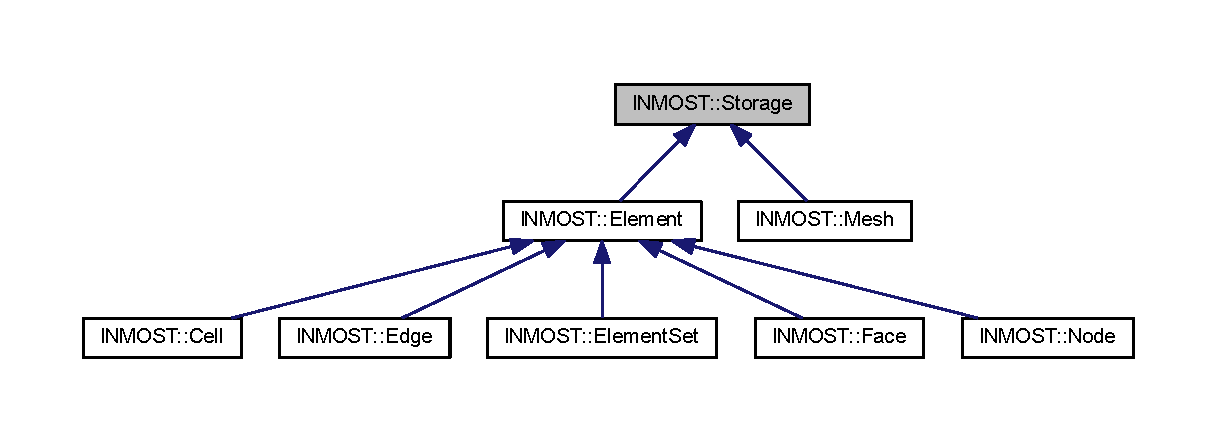
\includegraphics[width=350pt]{classINMOST_1_1Storage__inherit__graph}
\end{center}
\end{figure}
\subsection*{Classes}
\begin{DoxyCompactItemize}
\item 
class \hyperlink{classINMOST_1_1Storage_1_1reference__array}{reference\-\_\-array}
\begin{DoxyCompactList}\small\item\em \hyperlink{classINMOST_1_1Storage}{Storage} type for representing arrays of \hyperlink{classINMOST_1_1Element}{Element} references. \end{DoxyCompactList}\end{DoxyCompactItemize}
\subsection*{Public Types}
\begin{DoxyCompactItemize}
\item 
\hypertarget{classINMOST_1_1Storage_a853346784b4a5822a7fac54d8f10f805}{typedef I\-N\-M\-O\-S\-T\-\_\-\-D\-A\-T\-A\-\_\-\-R\-E\-A\-L\-\_\-\-T\-Y\-P\-E \hyperlink{classINMOST_1_1Storage_a853346784b4a5822a7fac54d8f10f805}{real}}\label{classINMOST_1_1Storage_a853346784b4a5822a7fac54d8f10f805}

\begin{DoxyCompactList}\small\item\em \hyperlink{classINMOST_1_1Storage}{Storage} type for representing real values. \end{DoxyCompactList}\item 
\hypertarget{classINMOST_1_1Storage_aec96942bc647417a801e2895b45964d2}{typedef I\-N\-M\-O\-S\-T\-\_\-\-D\-A\-T\-A\-\_\-\-I\-N\-T\-E\-G\-E\-R\-\_\-\-T\-Y\-P\-E \hyperlink{classINMOST_1_1Storage_aec96942bc647417a801e2895b45964d2}{integer}}\label{classINMOST_1_1Storage_aec96942bc647417a801e2895b45964d2}

\begin{DoxyCompactList}\small\item\em \hyperlink{classINMOST_1_1Storage}{Storage} type for representing integer values. \end{DoxyCompactList}\item 
\hypertarget{classINMOST_1_1Storage_ae429556af77094077d212e0ac23c8cfc}{typedef I\-N\-M\-O\-S\-T\-\_\-\-D\-A\-T\-A\-\_\-\-B\-U\-L\-K\-\_\-\-T\-Y\-P\-E \hyperlink{classINMOST_1_1Storage_ae429556af77094077d212e0ac23c8cfc}{bulk}}\label{classINMOST_1_1Storage_ae429556af77094077d212e0ac23c8cfc}

\begin{DoxyCompactList}\small\item\em \hyperlink{classINMOST_1_1Storage}{Storage} type for representing one byte of abstact data. \end{DoxyCompactList}\item 
\hypertarget{classINMOST_1_1Storage_ae333dfced6fa9cfde0c8e7dcf1b0cc2b}{typedef I\-N\-M\-O\-S\-T\-\_\-\-D\-A\-T\-A\-\_\-\-E\-N\-U\-M\-\_\-\-T\-Y\-P\-E \hyperlink{classINMOST_1_1Storage_ae333dfced6fa9cfde0c8e7dcf1b0cc2b}{enumerator}}\label{classINMOST_1_1Storage_ae333dfced6fa9cfde0c8e7dcf1b0cc2b}

\begin{DoxyCompactList}\small\item\em type for representing unsigned integer values. \end{DoxyCompactList}\item 
\hypertarget{classINMOST_1_1Storage_a8674802045ec170a3c9d0e3281545b54}{typedef Handle\-Type \hyperlink{classINMOST_1_1Storage_a8674802045ec170a3c9d0e3281545b54}{reference}}\label{classINMOST_1_1Storage_a8674802045ec170a3c9d0e3281545b54}

\begin{DoxyCompactList}\small\item\em \hyperlink{classINMOST_1_1Storage}{Storage} type for representing references to \hyperlink{classINMOST_1_1Element}{Element}. \end{DoxyCompactList}\item 
\hypertarget{classINMOST_1_1Storage_a430e5358d435befb38169beef593527e}{typedef shell$<$ \hyperlink{classINMOST_1_1Storage_a853346784b4a5822a7fac54d8f10f805}{real} $>$ \hyperlink{classINMOST_1_1Storage_a430e5358d435befb38169beef593527e}{real\-\_\-array}}\label{classINMOST_1_1Storage_a430e5358d435befb38169beef593527e}

\begin{DoxyCompactList}\small\item\em \hyperlink{classINMOST_1_1Storage}{Storage} type for representing arrays of real values. \end{DoxyCompactList}\item 
\hypertarget{classINMOST_1_1Storage_a4d1637367f0487eb778894b57fc94647}{typedef shell$<$ \hyperlink{classINMOST_1_1Storage_aec96942bc647417a801e2895b45964d2}{integer} $>$ \hyperlink{classINMOST_1_1Storage_a4d1637367f0487eb778894b57fc94647}{integer\-\_\-array}}\label{classINMOST_1_1Storage_a4d1637367f0487eb778894b57fc94647}

\begin{DoxyCompactList}\small\item\em \hyperlink{classINMOST_1_1Storage}{Storage} type for representing arrays of integer values. \end{DoxyCompactList}\item 
\hypertarget{classINMOST_1_1Storage_a6e49b2a38cb55dd59529bd23e8b1b852}{typedef shell$<$ \hyperlink{classINMOST_1_1Storage_ae429556af77094077d212e0ac23c8cfc}{bulk} $>$ \hyperlink{classINMOST_1_1Storage_a6e49b2a38cb55dd59529bd23e8b1b852}{bulk\-\_\-array}}\label{classINMOST_1_1Storage_a6e49b2a38cb55dd59529bd23e8b1b852}

\begin{DoxyCompactList}\small\item\em \hyperlink{classINMOST_1_1Storage}{Storage} type for representing abstact data as a series of bytes. \end{DoxyCompactList}\end{DoxyCompactItemize}
\subsection*{Public Member Functions}
\begin{DoxyCompactItemize}
\item 
\hypertarget{classINMOST_1_1Storage_adf1bf5a77779751b057db0d2a1d5defc}{{\bfseries Storage} (const \hyperlink{classINMOST_1_1Storage}{Storage} \&other)}\label{classINMOST_1_1Storage_adf1bf5a77779751b057db0d2a1d5defc}

\item 
\hypertarget{classINMOST_1_1Storage_ab54484f34481cbd2583588f7ca502521}{{\bfseries Storage} (\hyperlink{classINMOST_1_1Mesh}{Mesh} $\ast$mesh, Handle\-Type handle)}\label{classINMOST_1_1Storage_ab54484f34481cbd2583588f7ca502521}

\item 
\hypertarget{classINMOST_1_1Storage_a9fd7d01b2f05bf061ba8439fd1d25599}{\hyperlink{classINMOST_1_1Storage_a9fd7d01b2f05bf061ba8439fd1d25599}{Storage} (\hyperlink{classINMOST_1_1Mesh}{Mesh} $\ast$mesh, Handle\-Type $\ast$handle)}\label{classINMOST_1_1Storage_a9fd7d01b2f05bf061ba8439fd1d25599}

\begin{DoxyCompactList}\small\item\em This constructor allows for remote handle modification. \end{DoxyCompactList}\item 
\hypertarget{classINMOST_1_1Storage_a156c939c83d6854e1efaa29c1c38dddb}{\hyperlink{classINMOST_1_1Storage}{Storage} \& \hyperlink{classINMOST_1_1Storage_a156c939c83d6854e1efaa29c1c38dddb}{operator=} (\hyperlink{classINMOST_1_1Storage}{Storage} const \&other)}\label{classINMOST_1_1Storage_a156c939c83d6854e1efaa29c1c38dddb}

\begin{DoxyCompactList}\small\item\em If there is a link to handle provided (automatically by \hyperlink{classINMOST_1_1ElementArray}{Element\-Array} and \hyperlink{classINMOST_1_1Storage_1_1reference__array}{reference\-\_\-array}), then remote handle value will be modified. \end{DoxyCompactList}\item 
\hypertarget{classINMOST_1_1Storage_a2c3431bf6dbdbdfb4beaf2cac0f319a4}{bool {\bfseries operator==} (const \hyperlink{classINMOST_1_1Storage}{Storage} \&other)}\label{classINMOST_1_1Storage_a2c3431bf6dbdbdfb4beaf2cac0f319a4}

\item 
\hypertarget{classINMOST_1_1Storage_a4fdd5cda6a98308a3ac442b119a7c406}{bool {\bfseries operator!=} (const \hyperlink{classINMOST_1_1Storage}{Storage} \&other)}\label{classINMOST_1_1Storage_a4fdd5cda6a98308a3ac442b119a7c406}

\item 
\hypertarget{classINMOST_1_1Storage_aa53cbc67f9303555dc4fc657638b75e2}{\hyperlink{classINMOST_1_1Storage}{Storage} $\ast$ {\bfseries operator-\/$>$} ()}\label{classINMOST_1_1Storage_aa53cbc67f9303555dc4fc657638b75e2}

\item 
\hypertarget{classINMOST_1_1Storage_a7b258b0537667008d570b1ebfbdff1cc}{const \hyperlink{classINMOST_1_1Storage}{Storage} $\ast$ {\bfseries operator-\/$>$} () const }\label{classINMOST_1_1Storage_a7b258b0537667008d570b1ebfbdff1cc}

\item 
\hypertarget{classINMOST_1_1Storage_a74072ef234bfe67ed7f46f3adb3abf5a}{\hyperlink{classINMOST_1_1Storage}{Storage} \& {\bfseries self} ()}\label{classINMOST_1_1Storage_a74072ef234bfe67ed7f46f3adb3abf5a}

\item 
\hypertarget{classINMOST_1_1Storage_a30f75e7b6a5229dfbdbc946cba466ec4}{const \hyperlink{classINMOST_1_1Storage}{Storage} \& {\bfseries self} () const }\label{classINMOST_1_1Storage_a30f75e7b6a5229dfbdbc946cba466ec4}

\item 
\hypertarget{classINMOST_1_1Storage_ace95cd4dc7a18215d2b67fac8580dd52}{\hyperlink{classINMOST_1_1Storage_a853346784b4a5822a7fac54d8f10f805}{real} \& \hyperlink{classINMOST_1_1Storage_ace95cd4dc7a18215d2b67fac8580dd52}{Real} (const \hyperlink{classINMOST_1_1Tag}{Tag} \&tag) const }\label{classINMOST_1_1Storage_ace95cd4dc7a18215d2b67fac8580dd52}

\begin{DoxyCompactList}\small\item\em Retrieve real value associated with \hyperlink{classINMOST_1_1Tag}{Tag}. \end{DoxyCompactList}\item 
\hypertarget{classINMOST_1_1Storage_a802727f198dcfd7436fbc3a5080c6d88}{\hyperlink{classINMOST_1_1Storage_aec96942bc647417a801e2895b45964d2}{integer} \& \hyperlink{classINMOST_1_1Storage_a802727f198dcfd7436fbc3a5080c6d88}{Integer} (const \hyperlink{classINMOST_1_1Tag}{Tag} \&tag) const }\label{classINMOST_1_1Storage_a802727f198dcfd7436fbc3a5080c6d88}

\begin{DoxyCompactList}\small\item\em Retrieve integer value associated with \hyperlink{classINMOST_1_1Tag}{Tag}. \end{DoxyCompactList}\item 
\hypertarget{classINMOST_1_1Storage_a6df0b301d16530712d24d4a3c7ec4d3e}{\hyperlink{classINMOST_1_1Storage_ae429556af77094077d212e0ac23c8cfc}{bulk} \& \hyperlink{classINMOST_1_1Storage_a6df0b301d16530712d24d4a3c7ec4d3e}{Bulk} (const \hyperlink{classINMOST_1_1Tag}{Tag} \&tag) const }\label{classINMOST_1_1Storage_a6df0b301d16530712d24d4a3c7ec4d3e}

\begin{DoxyCompactList}\small\item\em Retrieve one byte of abstract data associated with \hyperlink{classINMOST_1_1Tag}{Tag}. \end{DoxyCompactList}\item 
\hypertarget{classINMOST_1_1Storage_a2433d2e9fdad1de2af584f4fbf318617}{\hyperlink{classINMOST_1_1Storage_a8674802045ec170a3c9d0e3281545b54}{reference} \& \hyperlink{classINMOST_1_1Storage_a2433d2e9fdad1de2af584f4fbf318617}{Reference} (const \hyperlink{classINMOST_1_1Tag}{Tag} \&tag) const }\label{classINMOST_1_1Storage_a2433d2e9fdad1de2af584f4fbf318617}

\begin{DoxyCompactList}\small\item\em Retrieve \hyperlink{classINMOST_1_1Element}{Element} reference associated with \hyperlink{classINMOST_1_1Tag}{Tag}. \end{DoxyCompactList}\item 
\hypertarget{classINMOST_1_1Storage_a45683e543b10f3ca94595fdbb43f2dd7}{\hyperlink{classINMOST_1_1Storage_a430e5358d435befb38169beef593527e}{real\-\_\-array} \hyperlink{classINMOST_1_1Storage_a45683e543b10f3ca94595fdbb43f2dd7}{Real\-Array} (const \hyperlink{classINMOST_1_1Tag}{Tag} \&tag) const }\label{classINMOST_1_1Storage_a45683e543b10f3ca94595fdbb43f2dd7}

\begin{DoxyCompactList}\small\item\em Retrieve array of real values associated with \hyperlink{classINMOST_1_1Tag}{Tag}. \end{DoxyCompactList}\item 
\hypertarget{classINMOST_1_1Storage_aee19d33f10109b8076ed722d03ef3d3b}{\hyperlink{classINMOST_1_1Storage_a4d1637367f0487eb778894b57fc94647}{integer\-\_\-array} \hyperlink{classINMOST_1_1Storage_aee19d33f10109b8076ed722d03ef3d3b}{Integer\-Array} (const \hyperlink{classINMOST_1_1Tag}{Tag} \&tag) const }\label{classINMOST_1_1Storage_aee19d33f10109b8076ed722d03ef3d3b}

\begin{DoxyCompactList}\small\item\em Retrieve array of integer values associated with \hyperlink{classINMOST_1_1Tag}{Tag}. \end{DoxyCompactList}\item 
\hypertarget{classINMOST_1_1Storage_ab06fda6f458c36197b5a05d9bee5b220}{\hyperlink{classINMOST_1_1Storage_a6e49b2a38cb55dd59529bd23e8b1b852}{bulk\-\_\-array} \hyperlink{classINMOST_1_1Storage_ab06fda6f458c36197b5a05d9bee5b220}{Bulk\-Array} (const \hyperlink{classINMOST_1_1Tag}{Tag} \&tag) const }\label{classINMOST_1_1Storage_ab06fda6f458c36197b5a05d9bee5b220}

\begin{DoxyCompactList}\small\item\em Retrieve abstract data associated with \hyperlink{classINMOST_1_1Tag}{Tag} as a series of bytes. \end{DoxyCompactList}\item 
\hypertarget{classINMOST_1_1Storage_ad4635fde0dc22cb26d52fce6cdff9247}{\hyperlink{classINMOST_1_1Storage_1_1reference__array}{reference\-\_\-array} \hyperlink{classINMOST_1_1Storage_ad4635fde0dc22cb26d52fce6cdff9247}{Reference\-Array} (const \hyperlink{classINMOST_1_1Tag}{Tag} \&tag) const }\label{classINMOST_1_1Storage_ad4635fde0dc22cb26d52fce6cdff9247}

\begin{DoxyCompactList}\small\item\em Retrieve array of \hyperlink{classINMOST_1_1Element}{Element} references associated with \hyperlink{classINMOST_1_1Tag}{Tag}. \end{DoxyCompactList}\item 
\hypertarget{classINMOST_1_1Storage_a86362a22500a13f4d5d982237df2455d}{\hyperlink{classINMOST_1_1Storage_a430e5358d435befb38169beef593527e}{real\-\_\-array} {\bfseries Real\-Array\-D\-F} (const \hyperlink{classINMOST_1_1Tag}{Tag} \&tag) const }\label{classINMOST_1_1Storage_a86362a22500a13f4d5d982237df2455d}

\item 
\hypertarget{classINMOST_1_1Storage_aaaa2b3a048dbc2202382064f7eea2e58}{\hyperlink{classINMOST_1_1Storage_a4d1637367f0487eb778894b57fc94647}{integer\-\_\-array} {\bfseries Integer\-Array\-D\-F} (const \hyperlink{classINMOST_1_1Tag}{Tag} \&tag) const }\label{classINMOST_1_1Storage_aaaa2b3a048dbc2202382064f7eea2e58}

\item 
\hypertarget{classINMOST_1_1Storage_aab0811a9fe56b68a571808a9e198f15c}{\hyperlink{classINMOST_1_1Storage_a6e49b2a38cb55dd59529bd23e8b1b852}{bulk\-\_\-array} {\bfseries Bulk\-Array\-D\-F} (const \hyperlink{classINMOST_1_1Tag}{Tag} \&tag) const }\label{classINMOST_1_1Storage_aab0811a9fe56b68a571808a9e198f15c}

\item 
\hypertarget{classINMOST_1_1Storage_a4cc35892f554c1bb4ca0bad03f64cef9}{\hyperlink{classINMOST_1_1Storage_1_1reference__array}{reference\-\_\-array} {\bfseries Reference\-Array\-D\-F} (const \hyperlink{classINMOST_1_1Tag}{Tag} \&tag) const }\label{classINMOST_1_1Storage_a4cc35892f554c1bb4ca0bad03f64cef9}

\item 
\hypertarget{classINMOST_1_1Storage_ac61c1fc5e91ff5bc3e009e01870d7ad9}{\hyperlink{classINMOST_1_1Storage_a853346784b4a5822a7fac54d8f10f805}{real} \& {\bfseries Real\-D\-F} (const \hyperlink{classINMOST_1_1Tag}{Tag} \&tag) const }\label{classINMOST_1_1Storage_ac61c1fc5e91ff5bc3e009e01870d7ad9}

\item 
\hypertarget{classINMOST_1_1Storage_ab9e72d878654feabe107a74b790b715e}{\hyperlink{classINMOST_1_1Storage_aec96942bc647417a801e2895b45964d2}{integer} \& {\bfseries Integer\-D\-F} (const \hyperlink{classINMOST_1_1Tag}{Tag} \&tag) const }\label{classINMOST_1_1Storage_ab9e72d878654feabe107a74b790b715e}

\item 
\hypertarget{classINMOST_1_1Storage_a0d96258748000b4ffd08e0c283757655}{\hyperlink{classINMOST_1_1Storage_ae429556af77094077d212e0ac23c8cfc}{bulk} \& {\bfseries Bulk\-D\-F} (const \hyperlink{classINMOST_1_1Tag}{Tag} \&tag) const }\label{classINMOST_1_1Storage_a0d96258748000b4ffd08e0c283757655}

\item 
\hypertarget{classINMOST_1_1Storage_a4a0a45cd8b835451b963d2d6789cc76b}{\hyperlink{classINMOST_1_1Storage_a8674802045ec170a3c9d0e3281545b54}{reference} \& {\bfseries Reference\-D\-F} (const \hyperlink{classINMOST_1_1Tag}{Tag} \&tag) const }\label{classINMOST_1_1Storage_a4a0a45cd8b835451b963d2d6789cc76b}

\item 
\hypertarget{classINMOST_1_1Storage_aaf94d4d967a234ee124615f54f9ae0a0}{\hyperlink{classINMOST_1_1Storage_a430e5358d435befb38169beef593527e}{real\-\_\-array} {\bfseries Real\-Array\-D\-V} (const \hyperlink{classINMOST_1_1Tag}{Tag} \&tag) const }\label{classINMOST_1_1Storage_aaf94d4d967a234ee124615f54f9ae0a0}

\item 
\hypertarget{classINMOST_1_1Storage_a9aca9f6585bdfdbbaa5e053a4a72bb70}{\hyperlink{classINMOST_1_1Storage_a4d1637367f0487eb778894b57fc94647}{integer\-\_\-array} {\bfseries Integer\-Array\-D\-V} (const \hyperlink{classINMOST_1_1Tag}{Tag} \&tag) const }\label{classINMOST_1_1Storage_a9aca9f6585bdfdbbaa5e053a4a72bb70}

\item 
\hypertarget{classINMOST_1_1Storage_aa78451cbe91031bb9ebdaeecba66658a}{\hyperlink{classINMOST_1_1Storage_a6e49b2a38cb55dd59529bd23e8b1b852}{bulk\-\_\-array} {\bfseries Bulk\-Array\-D\-V} (const \hyperlink{classINMOST_1_1Tag}{Tag} \&tag) const }\label{classINMOST_1_1Storage_aa78451cbe91031bb9ebdaeecba66658a}

\item 
\hypertarget{classINMOST_1_1Storage_afe4484db2915bc633bbc5310bc00ee8a}{\hyperlink{classINMOST_1_1Storage_1_1reference__array}{reference\-\_\-array} {\bfseries Reference\-Array\-D\-V} (const \hyperlink{classINMOST_1_1Tag}{Tag} \&tag) const }\label{classINMOST_1_1Storage_afe4484db2915bc633bbc5310bc00ee8a}

\item 
\hypertarget{classINMOST_1_1Storage_a19e5f595ccb081dfa09537a9f9abc570}{\hyperlink{classINMOST_1_1Storage_a853346784b4a5822a7fac54d8f10f805}{real} \& {\bfseries Real\-D\-V} (const \hyperlink{classINMOST_1_1Tag}{Tag} \&tag) const }\label{classINMOST_1_1Storage_a19e5f595ccb081dfa09537a9f9abc570}

\item 
\hypertarget{classINMOST_1_1Storage_a4a2f6952652596994f88cce7cc97604a}{\hyperlink{classINMOST_1_1Storage_aec96942bc647417a801e2895b45964d2}{integer} \& {\bfseries Integer\-D\-V} (const \hyperlink{classINMOST_1_1Tag}{Tag} \&tag) const }\label{classINMOST_1_1Storage_a4a2f6952652596994f88cce7cc97604a}

\item 
\hypertarget{classINMOST_1_1Storage_ad660844d3dad1ab9079065ef0e597b20}{\hyperlink{classINMOST_1_1Storage_ae429556af77094077d212e0ac23c8cfc}{bulk} \& {\bfseries Bulk\-D\-V} (const \hyperlink{classINMOST_1_1Tag}{Tag} \&tag) const }\label{classINMOST_1_1Storage_ad660844d3dad1ab9079065ef0e597b20}

\item 
\hypertarget{classINMOST_1_1Storage_a7432a2e64b3ac57860deb252087b2f66}{\hyperlink{classINMOST_1_1Storage_a8674802045ec170a3c9d0e3281545b54}{reference} \& {\bfseries Reference\-D\-V} (const \hyperlink{classINMOST_1_1Tag}{Tag} \&tag) const }\label{classINMOST_1_1Storage_a7432a2e64b3ac57860deb252087b2f66}

\item 
I\-N\-M\-O\-S\-T\-\_\-\-D\-A\-T\-A\-\_\-\-E\-N\-U\-M\-\_\-\-T\-Y\-P\-E \hyperlink{classINMOST_1_1Storage_a0c416b8e55014921426055508deca124}{Get\-Data\-Size} (const \hyperlink{classINMOST_1_1Tag}{Tag} \&tag) const 
\begin{DoxyCompactList}\small\item\em Return the data length associated with \hyperlink{classINMOST_1_1Tag}{Tag}. \end{DoxyCompactList}\item 
void \hyperlink{classINMOST_1_1Storage_af834468fb65cd43e272502985c050820}{Set\-Data\-Size} (const \hyperlink{classINMOST_1_1Tag}{Tag} \&tag, I\-N\-M\-O\-S\-T\-\_\-\-D\-A\-T\-A\-\_\-\-E\-N\-U\-M\-\_\-\-T\-Y\-P\-E new\-\_\-size) const 
\begin{DoxyCompactList}\small\item\em Set the length of data associated with \hyperlink{classINMOST_1_1Tag}{Tag}. \end{DoxyCompactList}\item 
void \hyperlink{classINMOST_1_1Storage_ae5dc4f3507b7f327fb29ae48311a4eea}{Get\-Data} (const \hyperlink{classINMOST_1_1Tag}{Tag} \&tag, I\-N\-M\-O\-S\-T\-\_\-\-D\-A\-T\-A\-\_\-\-E\-N\-U\-M\-\_\-\-T\-Y\-P\-E shift, I\-N\-M\-O\-S\-T\-\_\-\-D\-A\-T\-A\-\_\-\-E\-N\-U\-M\-\_\-\-T\-Y\-P\-E size, void $\ast$data) const 
\begin{DoxyCompactList}\small\item\em Extract part of the data associated with \hyperlink{classINMOST_1_1Tag}{Tag}. \end{DoxyCompactList}\item 
\hypertarget{classINMOST_1_1Storage_aeb8cae6a4325c80da00fe9c9befaf300}{void {\bfseries Set\-Data} (const \hyperlink{classINMOST_1_1Tag}{Tag} \&tag, I\-N\-M\-O\-S\-T\-\_\-\-D\-A\-T\-A\-\_\-\-E\-N\-U\-M\-\_\-\-T\-Y\-P\-E shift, I\-N\-M\-O\-S\-T\-\_\-\-D\-A\-T\-A\-\_\-\-E\-N\-U\-M\-\_\-\-T\-Y\-P\-E size, const void $\ast$data) const }\label{classINMOST_1_1Storage_aeb8cae6a4325c80da00fe9c9befaf300}

\item 
\hypertarget{classINMOST_1_1Storage_a1e09e97adc4e172ebef2738b3ee1e2e6}{void {\bfseries Del\-Data} (const \hyperlink{classINMOST_1_1Tag}{Tag} \&tag) const }\label{classINMOST_1_1Storage_a1e09e97adc4e172ebef2738b3ee1e2e6}

\item 
\hypertarget{classINMOST_1_1Storage_a9bea3510b025f9083dbccd1fbdb94607}{void \hyperlink{classINMOST_1_1Storage_a9bea3510b025f9083dbccd1fbdb94607}{Del\-Sparse\-Data} (const \hyperlink{classINMOST_1_1Tag}{Tag} \&tag) const }\label{classINMOST_1_1Storage_a9bea3510b025f9083dbccd1fbdb94607}

\begin{DoxyCompactList}\small\item\em Deallocates space allocated for sparse data, frees variable array if necessary. \end{DoxyCompactList}\item 
\hypertarget{classINMOST_1_1Storage_af528c745af38f31bf6b8b77c1eafdb8a}{void \hyperlink{classINMOST_1_1Storage_af528c745af38f31bf6b8b77c1eafdb8a}{Del\-Dense\-Data} (const \hyperlink{classINMOST_1_1Tag}{Tag} \&tag) const }\label{classINMOST_1_1Storage_af528c745af38f31bf6b8b77c1eafdb8a}

\begin{DoxyCompactList}\small\item\em Frees variable array or fills field with zeroes. \end{DoxyCompactList}\item 
\hypertarget{classINMOST_1_1Storage_ab94105e63f94f9799ff9a58280d0bf63}{bool \hyperlink{classINMOST_1_1Storage_ab94105e63f94f9799ff9a58280d0bf63}{Have\-Data} (const \hyperlink{classINMOST_1_1Tag}{Tag} \&tag) const }\label{classINMOST_1_1Storage_ab94105e63f94f9799ff9a58280d0bf63}

\begin{DoxyCompactList}\small\item\em Check if any data is associated with \hyperlink{classINMOST_1_1Tag}{Tag}. \end{DoxyCompactList}\item 
\hypertarget{classINMOST_1_1Storage_ae6928532b6665a12831d13293c4c7b31}{\-\_\-\-\_\-\-I\-N\-L\-I\-N\-E Element\-Type {\bfseries Get\-Element\-Type} () const }\label{classINMOST_1_1Storage_ae6928532b6665a12831d13293c4c7b31}

\item 
\hypertarget{classINMOST_1_1Storage_ae29350683bf09e402e0343f758f3e9d1}{\-\_\-\-\_\-\-I\-N\-L\-I\-N\-E \hyperlink{classINMOST_1_1Storage_aec96942bc647417a801e2895b45964d2}{integer} {\bfseries Get\-Element\-Num} () const }\label{classINMOST_1_1Storage_ae29350683bf09e402e0343f758f3e9d1}

\item 
\hypertarget{classINMOST_1_1Storage_a9786e860933f2ab0970010ab4bcfc567}{void {\bfseries Set\-Marker} (Marker\-Type n) const }\label{classINMOST_1_1Storage_a9786e860933f2ab0970010ab4bcfc567}

\item 
\hypertarget{classINMOST_1_1Storage_a8cfbb42c2b3e6dbe03894c48e0ab4639}{bool {\bfseries Get\-Marker} (Marker\-Type n) const }\label{classINMOST_1_1Storage_a8cfbb42c2b3e6dbe03894c48e0ab4639}

\item 
\hypertarget{classINMOST_1_1Storage_a4b31f315682afcdb92e70a29d840650a}{void {\bfseries Rem\-Marker} (Marker\-Type n) const }\label{classINMOST_1_1Storage_a4b31f315682afcdb92e70a29d840650a}

\item 
\hypertarget{classINMOST_1_1Storage_a32ea32f722414ba7422366078d3e71da}{void {\bfseries Clear\-Marker\-Space} () const }\label{classINMOST_1_1Storage_a32ea32f722414ba7422366078d3e71da}

\item 
\hypertarget{classINMOST_1_1Storage_ae571daade7e16b5cb436a677ef7e2e0a}{void {\bfseries Get\-Marker\-Space} (\hyperlink{classINMOST_1_1Storage_ae429556af77094077d212e0ac23c8cfc}{bulk} copy\mbox{[}Marker\-Fields\mbox{]}) const }\label{classINMOST_1_1Storage_ae571daade7e16b5cb436a677ef7e2e0a}

\item 
\hypertarget{classINMOST_1_1Storage_a059a9c404f886d00fecd580df5534dab}{void {\bfseries Set\-Marker\-Space} (\hyperlink{classINMOST_1_1Storage_ae429556af77094077d212e0ac23c8cfc}{bulk} source\mbox{[}Marker\-Fields\mbox{]}) const }\label{classINMOST_1_1Storage_a059a9c404f886d00fecd580df5534dab}

\item 
\hypertarget{classINMOST_1_1Storage_abe3cba66241f06792ef848b07b755508}{\-\_\-\-\_\-\-I\-N\-L\-I\-N\-E \hyperlink{classINMOST_1_1Storage_aec96942bc647417a801e2895b45964d2}{integer} {\bfseries Local\-I\-D} () const }\label{classINMOST_1_1Storage_abe3cba66241f06792ef848b07b755508}

\item 
\hypertarget{classINMOST_1_1Storage_a3c453aa013219304225d6d98fe84cab4}{\hyperlink{classINMOST_1_1Storage_aec96942bc647417a801e2895b45964d2}{integer} \hyperlink{classINMOST_1_1Storage_a3c453aa013219304225d6d98fe84cab4}{Data\-Local\-I\-D} () const }\label{classINMOST_1_1Storage_a3c453aa013219304225d6d98fe84cab4}

\begin{DoxyCompactList}\small\item\em This number is guaranteed to be between 0 and Mesh\-::\-Number\-Of(type of element) after Mesh\-::\-Reorder\-Empty. \end{DoxyCompactList}\item 
\hypertarget{classINMOST_1_1Storage_a75a725fd1d76cc5b7b8098080692c8ff}{bool {\bfseries is\-Valid} () const }\label{classINMOST_1_1Storage_a75a725fd1d76cc5b7b8098080692c8ff}

\item 
\hypertarget{classINMOST_1_1Storage_a17995aa90731fae234cb2897a52ce824}{\-\_\-\-\_\-\-I\-N\-L\-I\-N\-E \hyperlink{classINMOST_1_1Mesh}{Mesh} $\ast$ {\bfseries Get\-Mesh\-Link} () const }\label{classINMOST_1_1Storage_a17995aa90731fae234cb2897a52ce824}

\item 
\hypertarget{classINMOST_1_1Storage_ac79e3f3664b2ff21892f37bce0caa0e0}{\-\_\-\-\_\-\-I\-N\-L\-I\-N\-E Handle\-Type {\bfseries Get\-Handle} () const }\label{classINMOST_1_1Storage_ac79e3f3664b2ff21892f37bce0caa0e0}

\end{DoxyCompactItemize}
\subsection*{Protected Attributes}
\begin{DoxyCompactItemize}
\item 
\hypertarget{classINMOST_1_1Storage_a3a9a0f8e226821c92b8e5c253e4474be}{Handle\-Type {\bfseries handle}}\label{classINMOST_1_1Storage_a3a9a0f8e226821c92b8e5c253e4474be}

\item 
\hypertarget{classINMOST_1_1Storage_a14f2ee75267f3c967db30b79558360a5}{Handle\-Type $\ast$ {\bfseries handle\-\_\-link}}\label{classINMOST_1_1Storage_a14f2ee75267f3c967db30b79558360a5}

\end{DoxyCompactItemize}
\subsection*{Friends}
\begin{DoxyCompactItemize}
\item 
\hypertarget{classINMOST_1_1Storage_aa41a130f156b145bffb3f4b5172c4c93}{class {\bfseries Mesh}}\label{classINMOST_1_1Storage_aa41a130f156b145bffb3f4b5172c4c93}

\end{DoxyCompactItemize}


\subsection{Detailed Description}
Base class for \hyperlink{classINMOST_1_1Mesh}{Mesh}, \hyperlink{classINMOST_1_1Element}{Element}, and \hyperlink{classINMOST_1_1ElementSet}{Element\-Set} classes. 

This base class is used for the \hyperlink{classINMOST_1_1Mesh}{Mesh} class, as well as \hyperlink{classINMOST_1_1Element}{Element} classes, and \hyperlink{classINMOST_1_1ElementSet}{Element\-Set} class.

\hyperlink{classINMOST_1_1Storage}{Storage} class is used for representing different data objects in memory. Each data object is associated with corresponding \hyperlink{classINMOST_1_1Tag}{Tag}. 

\subsection{Member Function Documentation}
\hypertarget{classINMOST_1_1Storage_ae5dc4f3507b7f327fb29ae48311a4eea}{\index{I\-N\-M\-O\-S\-T\-::\-Storage@{I\-N\-M\-O\-S\-T\-::\-Storage}!Get\-Data@{Get\-Data}}
\index{Get\-Data@{Get\-Data}!INMOST::Storage@{I\-N\-M\-O\-S\-T\-::\-Storage}}
\subsubsection[{Get\-Data}]{\setlength{\rightskip}{0pt plus 5cm}void I\-N\-M\-O\-S\-T\-::\-Storage\-::\-Get\-Data (
\begin{DoxyParamCaption}
\item[{const {\bf Tag} \&}]{tag, }
\item[{I\-N\-M\-O\-S\-T\-\_\-\-D\-A\-T\-A\-\_\-\-E\-N\-U\-M\-\_\-\-T\-Y\-P\-E}]{shift, }
\item[{I\-N\-M\-O\-S\-T\-\_\-\-D\-A\-T\-A\-\_\-\-E\-N\-U\-M\-\_\-\-T\-Y\-P\-E}]{size, }
\item[{void $\ast$}]{data}
\end{DoxyParamCaption}
) const}}\label{classINMOST_1_1Storage_ae5dc4f3507b7f327fb29ae48311a4eea}


Extract part of the data associated with \hyperlink{classINMOST_1_1Tag}{Tag}. 

Copy part of the associated array or data to the destination memory. 
\begin{DoxyParams}{Parameters}
{\em tag} & Identifying \hyperlink{classINMOST_1_1Tag}{Tag}. \\
\hline
{\em shift} & Starting position of the copied data. For abstact data – number of bytes to skip, otherwise number of values to skip. \\
\hline
{\em size} & Number of elements to copy. For abstact data – number of bytes to copy, otherwise number of values to copy. \\
\hline
{\em data} & Destination position to copy data to. \\
\hline
\end{DoxyParams}
\begin{DoxySeeAlso}{See Also}
Storage\-::\-Set\-Data 
\end{DoxySeeAlso}
\hypertarget{classINMOST_1_1Storage_a0c416b8e55014921426055508deca124}{\index{I\-N\-M\-O\-S\-T\-::\-Storage@{I\-N\-M\-O\-S\-T\-::\-Storage}!Get\-Data\-Size@{Get\-Data\-Size}}
\index{Get\-Data\-Size@{Get\-Data\-Size}!INMOST::Storage@{I\-N\-M\-O\-S\-T\-::\-Storage}}
\subsubsection[{Get\-Data\-Size}]{\setlength{\rightskip}{0pt plus 5cm}I\-N\-M\-O\-S\-T\-\_\-\-D\-A\-T\-A\-\_\-\-E\-N\-U\-M\-\_\-\-T\-Y\-P\-E I\-N\-M\-O\-S\-T\-::\-Storage\-::\-Get\-Data\-Size (
\begin{DoxyParamCaption}
\item[{const {\bf Tag} \&}]{tag}
\end{DoxyParamCaption}
) const}}\label{classINMOST_1_1Storage_a0c416b8e55014921426055508deca124}


Return the data length associated with \hyperlink{classINMOST_1_1Tag}{Tag}. 

For abstract data return the number of bytes, otherwise return the length of associated array. \begin{DoxySeeAlso}{See Also}
\hyperlink{classINMOST_1_1Storage_af834468fb65cd43e272502985c050820}{Storage\-::\-Set\-Data\-Size} 
\end{DoxySeeAlso}
\hypertarget{classINMOST_1_1Storage_af834468fb65cd43e272502985c050820}{\index{I\-N\-M\-O\-S\-T\-::\-Storage@{I\-N\-M\-O\-S\-T\-::\-Storage}!Set\-Data\-Size@{Set\-Data\-Size}}
\index{Set\-Data\-Size@{Set\-Data\-Size}!INMOST::Storage@{I\-N\-M\-O\-S\-T\-::\-Storage}}
\subsubsection[{Set\-Data\-Size}]{\setlength{\rightskip}{0pt plus 5cm}void I\-N\-M\-O\-S\-T\-::\-Storage\-::\-Set\-Data\-Size (
\begin{DoxyParamCaption}
\item[{const {\bf Tag} \&}]{tag, }
\item[{I\-N\-M\-O\-S\-T\-\_\-\-D\-A\-T\-A\-\_\-\-E\-N\-U\-M\-\_\-\-T\-Y\-P\-E}]{new\-\_\-size}
\end{DoxyParamCaption}
) const}}\label{classINMOST_1_1Storage_af834468fb65cd43e272502985c050820}


Set the length of data associated with \hyperlink{classINMOST_1_1Tag}{Tag}. 


\begin{DoxyParams}{Parameters}
{\em tag} & Identifying \hyperlink{classINMOST_1_1Tag}{Tag}. \\
\hline
{\em new\-\_\-size} & The number of bytes for abstract data, otherwise the length of the array. \\
\hline
\end{DoxyParams}
\begin{DoxySeeAlso}{See Also}
\hyperlink{classINMOST_1_1Storage_a0c416b8e55014921426055508deca124}{Storage\-::\-Get\-Data\-Size} 
\end{DoxySeeAlso}


The documentation for this class was generated from the following file\-:\begin{DoxyCompactItemize}
\item 
inmost\-\_\-mesh.\-h\end{DoxyCompactItemize}

\hypertarget{structINMOST_1_1Automatizator_1_1table}{\section{I\-N\-M\-O\-S\-T\-:\-:Automatizator\-:\-:table Struct Reference}
\label{structINMOST_1_1Automatizator_1_1table}\index{I\-N\-M\-O\-S\-T\-::\-Automatizator\-::table@{I\-N\-M\-O\-S\-T\-::\-Automatizator\-::table}}
}
\subsection*{Public Member Functions}
\begin{DoxyCompactItemize}
\item 
\hypertarget{structINMOST_1_1Automatizator_1_1table_ad3e236635d555ed1d672e8906a6a3811}{I\-N\-M\-O\-S\-T\-\_\-\-D\-A\-T\-A\-\_\-\-E\-N\-U\-M\-\_\-\-T\-Y\-P\-E {\bfseries binary\-\_\-search} (I\-N\-M\-O\-S\-T\-\_\-\-D\-A\-T\-A\-\_\-\-R\-E\-A\-L\-\_\-\-T\-Y\-P\-E arg)}\label{structINMOST_1_1Automatizator_1_1table_ad3e236635d555ed1d672e8906a6a3811}

\item 
\hypertarget{structINMOST_1_1Automatizator_1_1table_a99806737e8ead515bde8cd616738dee7}{I\-N\-M\-O\-S\-T\-\_\-\-D\-A\-T\-A\-\_\-\-R\-E\-A\-L\-\_\-\-T\-Y\-P\-E {\bfseries get\-\_\-value} (I\-N\-M\-O\-S\-T\-\_\-\-D\-A\-T\-A\-\_\-\-R\-E\-A\-L\-\_\-\-T\-Y\-P\-E arg)}\label{structINMOST_1_1Automatizator_1_1table_a99806737e8ead515bde8cd616738dee7}

\item 
\hypertarget{structINMOST_1_1Automatizator_1_1table_aeddbb19e6dcaaa6b193422ac6932387b}{I\-N\-M\-O\-S\-T\-\_\-\-D\-A\-T\-A\-\_\-\-R\-E\-A\-L\-\_\-\-T\-Y\-P\-E {\bfseries get\-\_\-derivative} (I\-N\-M\-O\-S\-T\-\_\-\-D\-A\-T\-A\-\_\-\-R\-E\-A\-L\-\_\-\-T\-Y\-P\-E arg)}\label{structINMOST_1_1Automatizator_1_1table_aeddbb19e6dcaaa6b193422ac6932387b}

\item 
\hypertarget{structINMOST_1_1Automatizator_1_1table_add262de14f3347b10e16273c5ed3872f}{std\-::pair\\*
$<$ I\-N\-M\-O\-S\-T\-\_\-\-D\-A\-T\-A\-\_\-\-R\-E\-A\-L\-\_\-\-T\-Y\-P\-E, \\*
I\-N\-M\-O\-S\-T\-\_\-\-D\-A\-T\-A\-\_\-\-R\-E\-A\-L\-\_\-\-T\-Y\-P\-E $>$ {\bfseries get\-\_\-both} (I\-N\-M\-O\-S\-T\-\_\-\-D\-A\-T\-A\-\_\-\-R\-E\-A\-L\-\_\-\-T\-Y\-P\-E arg)}\label{structINMOST_1_1Automatizator_1_1table_add262de14f3347b10e16273c5ed3872f}

\end{DoxyCompactItemize}
\subsection*{Public Attributes}
\begin{DoxyCompactItemize}
\item 
\hypertarget{structINMOST_1_1Automatizator_1_1table_a203af5d89805c5657d7cbf4737b4636d}{std\-::string {\bfseries name}}\label{structINMOST_1_1Automatizator_1_1table_a203af5d89805c5657d7cbf4737b4636d}

\item 
\hypertarget{structINMOST_1_1Automatizator_1_1table_affb50f813846d78f671041406eea0d10}{I\-N\-M\-O\-S\-T\-\_\-\-D\-A\-T\-A\-\_\-\-R\-E\-A\-L\-\_\-\-T\-Y\-P\-E $\ast$ {\bfseries args}}\label{structINMOST_1_1Automatizator_1_1table_affb50f813846d78f671041406eea0d10}

\item 
\hypertarget{structINMOST_1_1Automatizator_1_1table_a85c68ce74998d98e405df153bd526730}{I\-N\-M\-O\-S\-T\-\_\-\-D\-A\-T\-A\-\_\-\-R\-E\-A\-L\-\_\-\-T\-Y\-P\-E $\ast$ {\bfseries vals}}\label{structINMOST_1_1Automatizator_1_1table_a85c68ce74998d98e405df153bd526730}

\item 
\hypertarget{structINMOST_1_1Automatizator_1_1table_a9c205c5870a155a245c42199fff8974a}{I\-N\-M\-O\-S\-T\-\_\-\-D\-A\-T\-A\-\_\-\-E\-N\-U\-M\-\_\-\-T\-Y\-P\-E {\bfseries size}}\label{structINMOST_1_1Automatizator_1_1table_a9c205c5870a155a245c42199fff8974a}

\end{DoxyCompactItemize}


The documentation for this struct was generated from the following file\-:\begin{DoxyCompactItemize}
\item 
inmost\-\_\-autodiff.\-h\end{DoxyCompactItemize}

\hypertarget{classINMOST_1_1Tag}{\section{I\-N\-M\-O\-S\-T\-:\-:Tag Class Reference}
\label{classINMOST_1_1Tag}\index{I\-N\-M\-O\-S\-T\-::\-Tag@{I\-N\-M\-O\-S\-T\-::\-Tag}}
}
\subsection*{Public Member Functions}
\begin{DoxyCompactItemize}
\item 
\hypertarget{classINMOST_1_1Tag_a76f39e35a89e23996215d11344712305}{{\bfseries Tag} (const \hyperlink{classINMOST_1_1Tag}{Tag} \&other)}\label{classINMOST_1_1Tag_a76f39e35a89e23996215d11344712305}

\item 
\hypertarget{classINMOST_1_1Tag_a846728fecce1eaa7f3573694ee54cfb4}{bool {\bfseries operator$<$} (const \hyperlink{classINMOST_1_1Tag}{Tag} \&other) const }\label{classINMOST_1_1Tag_a846728fecce1eaa7f3573694ee54cfb4}

\item 
\hypertarget{classINMOST_1_1Tag_ae52dd043a4cb4cbe0aafefd304604e9c}{bool {\bfseries operator$>$} (const \hyperlink{classINMOST_1_1Tag}{Tag} \&other) const }\label{classINMOST_1_1Tag_ae52dd043a4cb4cbe0aafefd304604e9c}

\item 
\hypertarget{classINMOST_1_1Tag_aee3e7bd565322c36d6e4babeabccad08}{bool {\bfseries operator==} (const \hyperlink{classINMOST_1_1Tag}{Tag} \&other) const }\label{classINMOST_1_1Tag_aee3e7bd565322c36d6e4babeabccad08}

\item 
\hypertarget{classINMOST_1_1Tag_aebfdb3de0a85dfd92232e68cb763b514}{bool {\bfseries operator!=} (const \hyperlink{classINMOST_1_1Tag}{Tag} \&other) const }\label{classINMOST_1_1Tag_aebfdb3de0a85dfd92232e68cb763b514}

\item 
\hypertarget{classINMOST_1_1Tag_a826d9625e7f39ef4916f5fb6878cd048}{\hyperlink{classINMOST_1_1Tag}{Tag} \& {\bfseries operator=} (\hyperlink{classINMOST_1_1Tag}{Tag} const \&other)}\label{classINMOST_1_1Tag_a826d9625e7f39ef4916f5fb6878cd048}

\item 
\hypertarget{classINMOST_1_1Tag_a2a6d8f1e2efab36e317c7aa9467d18bb}{\-\_\-\-\_\-\-I\-N\-L\-I\-N\-E Data\-Type {\bfseries Get\-Data\-Type} () const }\label{classINMOST_1_1Tag_a2a6d8f1e2efab36e317c7aa9467d18bb}

\item 
\hypertarget{classINMOST_1_1Tag_ad21265a8333fa926aec279374881511c}{\-\_\-\-\_\-\-I\-N\-L\-I\-N\-E I\-N\-M\-O\-S\-T\-\_\-\-M\-P\-I\-\_\-\-Type {\bfseries Get\-Bulk\-Data\-Type} () const }\label{classINMOST_1_1Tag_ad21265a8333fa926aec279374881511c}

\item 
\hypertarget{classINMOST_1_1Tag_a98e30737d0fd1ce864fca88106bf4aa0}{\-\_\-\-\_\-\-I\-N\-L\-I\-N\-E I\-N\-M\-O\-S\-T\-\_\-\-D\-A\-T\-A\-\_\-\-E\-N\-U\-M\-\_\-\-T\-Y\-P\-E {\bfseries Get\-Bytes\-Size} () const }\label{classINMOST_1_1Tag_a98e30737d0fd1ce864fca88106bf4aa0}

\item 
\hypertarget{classINMOST_1_1Tag_ae74774d21aaf2dd820d2a5ea1bb43f9d}{\-\_\-\-\_\-\-I\-N\-L\-I\-N\-E I\-N\-M\-O\-S\-T\-\_\-\-D\-A\-T\-A\-\_\-\-E\-N\-U\-M\-\_\-\-T\-Y\-P\-E {\bfseries Get\-Size} () const }\label{classINMOST_1_1Tag_ae74774d21aaf2dd820d2a5ea1bb43f9d}

\item 
\hypertarget{classINMOST_1_1Tag_acc819bbeee997e187b3da9b07a703543}{\-\_\-\-\_\-\-I\-N\-L\-I\-N\-E std\-::string {\bfseries Get\-Tag\-Name} () const }\label{classINMOST_1_1Tag_acc819bbeee997e187b3da9b07a703543}

\item 
\hypertarget{classINMOST_1_1Tag_aef6923542b80e0e8ec121f8f95eeb5b7}{\-\_\-\-\_\-\-I\-N\-L\-I\-N\-E bool {\bfseries is\-Defined} (Element\-Type type) const }\label{classINMOST_1_1Tag_aef6923542b80e0e8ec121f8f95eeb5b7}

\item 
\hypertarget{classINMOST_1_1Tag_a0151597a4ccd7f9ad8ffe3b4774c2040}{\-\_\-\-\_\-\-I\-N\-L\-I\-N\-E bool {\bfseries is\-Sparse} (Element\-Type type) const }\label{classINMOST_1_1Tag_a0151597a4ccd7f9ad8ffe3b4774c2040}

\item 
\hypertarget{classINMOST_1_1Tag_a49c1f08eeb172434cd6f35fd3d4fd35c}{\-\_\-\-\_\-\-I\-N\-L\-I\-N\-E bool {\bfseries is\-Valid} () const }\label{classINMOST_1_1Tag_a49c1f08eeb172434cd6f35fd3d4fd35c}

\item 
\hypertarget{classINMOST_1_1Tag_a28fb2801ba18b08e8b10a927a01f53f8}{\-\_\-\-\_\-\-I\-N\-L\-I\-N\-E \hyperlink{classINMOST_1_1Mesh}{Mesh} $\ast$ {\bfseries Get\-Mesh\-Link} () const }\label{classINMOST_1_1Tag_a28fb2801ba18b08e8b10a927a01f53f8}

\item 
\hypertarget{classINMOST_1_1Tag_a93a0cb0d316f8496372276727c0a070d}{\-\_\-\-\_\-\-I\-N\-L\-I\-N\-E bool {\bfseries is\-Sparse\-By\-Dim} (I\-N\-M\-O\-S\-T\-\_\-\-D\-A\-T\-A\-\_\-\-I\-N\-T\-E\-G\-E\-R\-\_\-\-T\-Y\-P\-E typenum) const }\label{classINMOST_1_1Tag_a93a0cb0d316f8496372276727c0a070d}

\item 
\hypertarget{classINMOST_1_1Tag_a33a5c5e9c29033606b4b88ddbae20187}{\-\_\-\-\_\-\-I\-N\-L\-I\-N\-E bool {\bfseries is\-Defined\-By\-Dim} (I\-N\-M\-O\-S\-T\-\_\-\-D\-A\-T\-A\-\_\-\-I\-N\-T\-E\-G\-E\-R\-\_\-\-T\-Y\-P\-E typenum) const }\label{classINMOST_1_1Tag_a33a5c5e9c29033606b4b88ddbae20187}

\item 
\hypertarget{classINMOST_1_1Tag_a6007500c34ab4ddffd9a0283678d0ba6}{\-\_\-\-\_\-\-I\-N\-L\-I\-N\-E void {\bfseries Set\-Bulk\-Data\-Type} (I\-N\-M\-O\-S\-T\-\_\-\-M\-P\-I\-\_\-\-Type type)}\label{classINMOST_1_1Tag_a6007500c34ab4ddffd9a0283678d0ba6}

\end{DoxyCompactItemize}
\subsection*{Friends}
\begin{DoxyCompactItemize}
\item 
\hypertarget{classINMOST_1_1Tag_a49b2688bfa740d6565767541de3bd180}{class {\bfseries Tag\-Manager}}\label{classINMOST_1_1Tag_a49b2688bfa740d6565767541de3bd180}

\item 
\hypertarget{classINMOST_1_1Tag_ab647623b3295040f83d3afb2a502a223}{class {\bfseries Storage}}\label{classINMOST_1_1Tag_ab647623b3295040f83d3afb2a502a223}

\item 
\hypertarget{classINMOST_1_1Tag_aa41a130f156b145bffb3f4b5172c4c93}{class {\bfseries Mesh}}\label{classINMOST_1_1Tag_aa41a130f156b145bffb3f4b5172c4c93}

\end{DoxyCompactItemize}


The documentation for this class was generated from the following file\-:\begin{DoxyCompactItemize}
\item 
inmost\-\_\-mesh.\-h\end{DoxyCompactItemize}

\hypertarget{classINMOST_1_1TagManager}{\section{I\-N\-M\-O\-S\-T\-:\-:Tag\-Manager Class Reference}
\label{classINMOST_1_1TagManager}\index{I\-N\-M\-O\-S\-T\-::\-Tag\-Manager@{I\-N\-M\-O\-S\-T\-::\-Tag\-Manager}}
}


Inheritance diagram for I\-N\-M\-O\-S\-T\-:\-:Tag\-Manager\-:
\subsection*{Classes}
\begin{DoxyCompactItemize}
\item 
struct \hyperlink{structINMOST_1_1TagManager_1_1sparse__sub__record}{sparse\-\_\-sub\-\_\-record}
\end{DoxyCompactItemize}
\subsection*{Public Types}
\begin{DoxyCompactItemize}
\item 
\hypertarget{classINMOST_1_1TagManager_adda9f59b50509dee56fa03697e1b4b02}{typedef tag\-\_\-array\-\_\-type\-::iterator {\bfseries iterator\-Tag}}\label{classINMOST_1_1TagManager_adda9f59b50509dee56fa03697e1b4b02}

\end{DoxyCompactItemize}
\subsection*{Public Member Functions}
\begin{DoxyCompactItemize}
\item 
\hypertarget{classINMOST_1_1TagManager_a61d1c149756989d61868d41e374d7c76}{bool {\bfseries Have\-Tag} (std\-::string name) const }\label{classINMOST_1_1TagManager_a61d1c149756989d61868d41e374d7c76}

\item 
\hypertarget{classINMOST_1_1TagManager_aeadbec8cfb140793eb5a594649ba0247}{\hyperlink{classINMOST_1_1Tag}{Tag} {\bfseries Get\-Tag} (std\-::string name) const }\label{classINMOST_1_1TagManager_aeadbec8cfb140793eb5a594649ba0247}

\item 
\hypertarget{classINMOST_1_1TagManager_a5bb782655ad079208d1b2b6e614d0499}{void {\bfseries List\-Tag\-Names} (std\-::vector$<$ std\-::string $>$ \&list) const }\label{classINMOST_1_1TagManager_a5bb782655ad079208d1b2b6e614d0499}

\item 
\hypertarget{classINMOST_1_1TagManager_ac85b7509d389191f59772bf5defc931b}{\hyperlink{classINMOST_1_1Tag}{Tag} {\bfseries Create\-Tag} (\hyperlink{classINMOST_1_1Mesh}{Mesh} $\ast$m, std\-::string name, Data\-Type dtype, Element\-Type etype, Element\-Type sparse, I\-N\-M\-O\-S\-T\-\_\-\-D\-A\-T\-A\-\_\-\-E\-N\-U\-M\-\_\-\-T\-Y\-P\-E size=E\-N\-U\-M\-U\-N\-D\-E\-F)}\label{classINMOST_1_1TagManager_ac85b7509d389191f59772bf5defc931b}

\item 
\hypertarget{classINMOST_1_1TagManager_aff704532d5a261a3e6572c84f54d14c8}{virtual \hyperlink{classINMOST_1_1Tag}{Tag} {\bfseries Delete\-Tag} (\hyperlink{classINMOST_1_1Tag}{Tag} tag, Element\-Type mask)}\label{classINMOST_1_1TagManager_aff704532d5a261a3e6572c84f54d14c8}

\item 
\hypertarget{classINMOST_1_1TagManager_a320c0dbd9ead879cc09e3c497b95b954}{bool {\bfseries Element\-Defined} (\hyperlink{classINMOST_1_1Tag}{Tag} const \&tag, Element\-Type etype) const }\label{classINMOST_1_1TagManager_a320c0dbd9ead879cc09e3c497b95b954}

\end{DoxyCompactItemize}
\subsection*{Protected Types}
\begin{DoxyCompactItemize}
\item 
\hypertarget{classINMOST_1_1TagManager_a6c89e8450f65055147301406d7f9c437}{typedef chunk\-\_\-array\\*
$<$ I\-N\-M\-O\-S\-T\-\_\-\-D\-A\-T\-A\-\_\-\-E\-N\-U\-M\-\_\-\-T\-Y\-P\-E, \\*
chunk\-\_\-bits\-\_\-empty $>$ {\bfseries empty\-\_\-data}}\label{classINMOST_1_1TagManager_a6c89e8450f65055147301406d7f9c437}

\item 
\hypertarget{classINMOST_1_1TagManager_ab7915f5a3e87fe36e14e9766d1437369}{typedef chunk\-\_\-array$<$ \hyperlink{classINMOST_1_1Tag}{Tag}, \\*
chunk\-\_\-bits\-\_\-tags $>$ {\bfseries tag\-\_\-array\-\_\-type}}\label{classINMOST_1_1TagManager_ab7915f5a3e87fe36e14e9766d1437369}

\item 
\hypertarget{classINMOST_1_1TagManager_acc5a035bf2ee39c0fb8417b0b290a26b}{typedef chunk\-\_\-bulk\-\_\-array\\*
$<$ chunk\-\_\-bits\-\_\-elems $>$ {\bfseries dense\-\_\-sub\-\_\-type}}\label{classINMOST_1_1TagManager_acc5a035bf2ee39c0fb8417b0b290a26b}

\item 
\hypertarget{classINMOST_1_1TagManager_ac573af6facd80a651b3496938235130e}{typedef chunk\-\_\-array\\*
$<$ dense\-\_\-sub\-\_\-type, \\*
chunk\-\_\-bits\-\_\-dense\-\_\-array $>$ {\bfseries dense\-\_\-data\-\_\-array\-\_\-type}}\label{classINMOST_1_1TagManager_ac573af6facd80a651b3496938235130e}

\item 
\hypertarget{classINMOST_1_1TagManager_a580e8cfe488c581a007d7108a27d5718}{typedef array$<$ \hyperlink{structINMOST_1_1TagManager_1_1sparse__sub__record}{sparse\-\_\-sub\-\_\-record} $>$ {\bfseries sparse\-\_\-sub\-\_\-type}}\label{classINMOST_1_1TagManager_a580e8cfe488c581a007d7108a27d5718}

\item 
\hypertarget{classINMOST_1_1TagManager_a36d8c18c51b82ff914061a3a13b16444}{typedef chunk\-\_\-array\\*
$<$ sparse\-\_\-sub\-\_\-type, \\*
chunk\-\_\-bits\-\_\-elems $>$ {\bfseries sparse\-\_\-data\-\_\-array\-\_\-type}}\label{classINMOST_1_1TagManager_a36d8c18c51b82ff914061a3a13b16444}

\item 
\hypertarget{classINMOST_1_1TagManager_a6516013a33fc678ce51ee7a9566ffc9b}{typedef chunk\-\_\-array\\*
$<$ I\-N\-M\-O\-S\-T\-\_\-\-D\-A\-T\-A\-\_\-\-I\-N\-T\-E\-G\-E\-R\-\_\-\-T\-Y\-P\-E, \\*
chunk\-\_\-bits\-\_\-elems $>$ {\bfseries back\-\_\-links\-\_\-type}}\label{classINMOST_1_1TagManager_a6516013a33fc678ce51ee7a9566ffc9b}

\item 
\hypertarget{classINMOST_1_1TagManager_a083c5b8cf529631c183d8663e69e6527}{typedef tag\-\_\-array\-\_\-type\-::iterator {\bfseries tag\-\_\-iterator}}\label{classINMOST_1_1TagManager_a083c5b8cf529631c183d8663e69e6527}

\item 
\hypertarget{classINMOST_1_1TagManager_a84ab39af175e4d73ca4b9a9a7915401a}{typedef \\*
tag\-\_\-array\-\_\-type\-::const\-\_\-iterator {\bfseries tag\-\_\-const\-\_\-iterator}}\label{classINMOST_1_1TagManager_a84ab39af175e4d73ca4b9a9a7915401a}

\end{DoxyCompactItemize}
\subsection*{Protected Member Functions}
\begin{DoxyCompactItemize}
\item 
\hypertarget{classINMOST_1_1TagManager_a74c7e50f03649a1b5041f524d0421079}{{\bfseries Tag\-Manager} (const \hyperlink{classINMOST_1_1TagManager}{Tag\-Manager} \&other)}\label{classINMOST_1_1TagManager_a74c7e50f03649a1b5041f524d0421079}

\item 
\hypertarget{classINMOST_1_1TagManager_ab128149e17df47b9ebfdb8c4997a46c4}{\hyperlink{classINMOST_1_1TagManager}{Tag\-Manager} \& {\bfseries operator=} (\hyperlink{classINMOST_1_1TagManager}{Tag\-Manager} const \&other)}\label{classINMOST_1_1TagManager_ab128149e17df47b9ebfdb8c4997a46c4}

\item 
\hypertarget{classINMOST_1_1TagManager_a60a6f61fd31686e47ddda096cd5a458b}{void {\bfseries Reallocate\-Data} (const \hyperlink{classINMOST_1_1Tag}{Tag} \&t, I\-N\-M\-O\-S\-T\-\_\-\-D\-A\-T\-A\-\_\-\-I\-N\-T\-E\-G\-E\-R\-\_\-\-T\-Y\-P\-E etypenum, I\-N\-M\-O\-S\-T\-\_\-\-D\-A\-T\-A\-\_\-\-E\-N\-U\-M\-\_\-\-T\-Y\-P\-E new\-\_\-size)}\label{classINMOST_1_1TagManager_a60a6f61fd31686e47ddda096cd5a458b}

\item 
\hypertarget{classINMOST_1_1TagManager_a397a04c1c4545b1152a438acc432f952}{void {\bfseries Reallocate\-Data} (I\-N\-M\-O\-S\-T\-\_\-\-D\-A\-T\-A\-\_\-\-I\-N\-T\-E\-G\-E\-R\-\_\-\-T\-Y\-P\-E etypenum, I\-N\-M\-O\-S\-T\-\_\-\-D\-A\-T\-A\-\_\-\-E\-N\-U\-M\-\_\-\-T\-Y\-P\-E new\-\_\-size)}\label{classINMOST_1_1TagManager_a397a04c1c4545b1152a438acc432f952}

\item 
\hypertarget{classINMOST_1_1TagManager_a3c7825981150daf50fb56d4f189e7c4e}{\-\_\-\-\_\-\-I\-N\-L\-I\-N\-E sparse\-\_\-sub\-\_\-type const \& {\bfseries Get\-Sparse\-Data} (int etypenum, int local\-\_\-id) const }\label{classINMOST_1_1TagManager_a3c7825981150daf50fb56d4f189e7c4e}

\item 
\hypertarget{classINMOST_1_1TagManager_ab95230b841496e62ea1a645b3d1336ce}{\-\_\-\-\_\-\-I\-N\-L\-I\-N\-E sparse\-\_\-sub\-\_\-type \& {\bfseries Get\-Sparse\-Data} (int etypenum, int local\-\_\-id)}\label{classINMOST_1_1TagManager_ab95230b841496e62ea1a645b3d1336ce}

\item 
\hypertarget{classINMOST_1_1TagManager_a029c2b2db435c0d325eb272b598816d6}{\-\_\-\-\_\-\-I\-N\-L\-I\-N\-E dense\-\_\-sub\-\_\-type const \& {\bfseries Get\-Dense\-Data} (int pos) const }\label{classINMOST_1_1TagManager_a029c2b2db435c0d325eb272b598816d6}

\item 
\hypertarget{classINMOST_1_1TagManager_af98cc766513cd82c1f0a99c78c5b8528}{\-\_\-\-\_\-\-I\-N\-L\-I\-N\-E dense\-\_\-sub\-\_\-type \& {\bfseries Get\-Dense\-Data} (int pos)}\label{classINMOST_1_1TagManager_af98cc766513cd82c1f0a99c78c5b8528}

\end{DoxyCompactItemize}
\subsection*{Static Protected Member Functions}
\begin{DoxyCompactItemize}
\item 
\hypertarget{classINMOST_1_1TagManager_a3646206503d7c8bc5a7d1ab2f2550798}{static void {\bfseries Copy\-Data} (const \hyperlink{classINMOST_1_1Tag}{Tag} \&t, void $\ast$adata, const void $\ast$bdata)}\label{classINMOST_1_1TagManager_a3646206503d7c8bc5a7d1ab2f2550798}

\item 
\hypertarget{classINMOST_1_1TagManager_aa41305bccd3e4be8bfd5ff0b8246c807}{static void {\bfseries Destroy\-Variable\-Data} (const \hyperlink{classINMOST_1_1Tag}{Tag} \&t, void $\ast$adata)}\label{classINMOST_1_1TagManager_aa41305bccd3e4be8bfd5ff0b8246c807}

\end{DoxyCompactItemize}
\subsection*{Protected Attributes}
\begin{DoxyCompactItemize}
\item 
\hypertarget{classINMOST_1_1TagManager_ac92171533d42711a11684c52f6dfa737}{tag\-\_\-array\-\_\-type {\bfseries tags}}\label{classINMOST_1_1TagManager_ac92171533d42711a11684c52f6dfa737}

\item 
\hypertarget{classINMOST_1_1TagManager_ac6f6cb319ebef941d38a8e2c8f17db94}{empty\-\_\-data {\bfseries empty\-\_\-dense\-\_\-data}}\label{classINMOST_1_1TagManager_ac6f6cb319ebef941d38a8e2c8f17db94}

\item 
\hypertarget{classINMOST_1_1TagManager_abaf73c1edda087f369ef969b64e6d9a1}{dense\-\_\-data\-\_\-array\-\_\-type {\bfseries dense\-\_\-data}}\label{classINMOST_1_1TagManager_abaf73c1edda087f369ef969b64e6d9a1}

\item 
\hypertarget{classINMOST_1_1TagManager_ad4fada89bccb1b59070868d0509cf70e}{sparse\-\_\-data\-\_\-array\-\_\-type {\bfseries sparse\-\_\-data} \mbox{[}6\mbox{]}}\label{classINMOST_1_1TagManager_ad4fada89bccb1b59070868d0509cf70e}

\item 
\hypertarget{classINMOST_1_1TagManager_aa9676936366e5777fa061e22ea6672ca}{back\-\_\-links\-\_\-type {\bfseries back\-\_\-links} \mbox{[}6\mbox{]}}\label{classINMOST_1_1TagManager_aa9676936366e5777fa061e22ea6672ca}

\end{DoxyCompactItemize}


The documentation for this class was generated from the following file\-:\begin{DoxyCompactItemize}
\item 
inmost\-\_\-mesh.\-h\end{DoxyCompactItemize}

\hypertarget{classINMOST_1_1TagMemory}{\section{I\-N\-M\-O\-S\-T\-:\-:Tag\-Memory Class Reference}
\label{classINMOST_1_1TagMemory}\index{I\-N\-M\-O\-S\-T\-::\-Tag\-Memory@{I\-N\-M\-O\-S\-T\-::\-Tag\-Memory}}
}
\subsection*{Public Member Functions}
\begin{DoxyCompactItemize}
\item 
\hypertarget{classINMOST_1_1TagMemory_ac07aafafbfda25b163f64cb6d3b7cec4}{{\bfseries Tag\-Memory} (\hyperlink{classINMOST_1_1Mesh}{Mesh} $\ast$m, const \hyperlink{classINMOST_1_1TagMemory}{Tag\-Memory} \&other)}\label{classINMOST_1_1TagMemory_ac07aafafbfda25b163f64cb6d3b7cec4}

\item 
\hypertarget{classINMOST_1_1TagMemory_a9e54be3865bc8f02c512292c924f840c}{\hyperlink{classINMOST_1_1TagMemory}{Tag\-Memory} \& {\bfseries operator=} (\hyperlink{classINMOST_1_1TagMemory}{Tag\-Memory} const \&other)}\label{classINMOST_1_1TagMemory_a9e54be3865bc8f02c512292c924f840c}

\end{DoxyCompactItemize}
\subsection*{Friends}
\begin{DoxyCompactItemize}
\item 
\hypertarget{classINMOST_1_1TagMemory_afc8c1b0e7f1fedf25715bd33b74eb56c}{class {\bfseries Tag}}\label{classINMOST_1_1TagMemory_afc8c1b0e7f1fedf25715bd33b74eb56c}

\item 
\hypertarget{classINMOST_1_1TagMemory_ab647623b3295040f83d3afb2a502a223}{class {\bfseries Storage}}\label{classINMOST_1_1TagMemory_ab647623b3295040f83d3afb2a502a223}

\end{DoxyCompactItemize}


The documentation for this class was generated from the following file\-:\begin{DoxyCompactItemize}
\item 
inmost\-\_\-mesh.\-h\end{DoxyCompactItemize}

\hypertarget{classINMOST_1_1Solver_1_1Vector}{\section{I\-N\-M\-O\-S\-T\-:\-:Solver\-:\-:Vector Class Reference}
\label{classINMOST_1_1Solver_1_1Vector}\index{I\-N\-M\-O\-S\-T\-::\-Solver\-::\-Vector@{I\-N\-M\-O\-S\-T\-::\-Solver\-::\-Vector}}
}


Distributed vector class.  




{\ttfamily \#include $<$inmost\-\_\-solver.\-h$>$}

\subsection*{Public Types}
\begin{DoxyCompactItemize}
\item 
\hypertarget{classINMOST_1_1Solver_1_1Vector_aa6542e5c0e63c5df96177efa8e57baf6}{typedef interval\\*
$<$ I\-N\-M\-O\-S\-T\-\_\-\-D\-A\-T\-A\-\_\-\-E\-N\-U\-M\-\_\-\-T\-Y\-P\-E, \\*
I\-N\-M\-O\-S\-T\-\_\-\-D\-A\-T\-A\-\_\-\-R\-E\-A\-L\-\_\-\-T\-Y\-P\-E $>$ {\bfseries Entries}}\label{classINMOST_1_1Solver_1_1Vector_aa6542e5c0e63c5df96177efa8e57baf6}

\item 
\hypertarget{classINMOST_1_1Solver_1_1Vector_aac42d705099eaecd6ac7435d09f51f3d}{typedef Entries\-::iterator {\bfseries iterator}}\label{classINMOST_1_1Solver_1_1Vector_aac42d705099eaecd6ac7435d09f51f3d}

\item 
\hypertarget{classINMOST_1_1Solver_1_1Vector_a6ddbd17be9dcfc1785b623aa40ff7391}{typedef Entries\-::const\-\_\-iterator {\bfseries const\-\_\-iterator}}\label{classINMOST_1_1Solver_1_1Vector_a6ddbd17be9dcfc1785b623aa40ff7391}

\end{DoxyCompactItemize}
\subsection*{Public Member Functions}
\begin{DoxyCompactItemize}
\item 
\hyperlink{classINMOST_1_1Solver_1_1Vector_a26af3465ba1e8abe8c3b3ed87782bffe}{Vector} (std\-::string \-\_\-name=\char`\"{}\char`\"{}, I\-N\-M\-O\-S\-T\-\_\-\-D\-A\-T\-A\-\_\-\-E\-N\-U\-M\-\_\-\-T\-Y\-P\-E start=0, I\-N\-M\-O\-S\-T\-\_\-\-D\-A\-T\-A\-\_\-\-E\-N\-U\-M\-\_\-\-T\-Y\-P\-E end=0, I\-N\-M\-O\-S\-T\-\_\-\-M\-P\-I\-\_\-\-Comm \-\_\-comm=I\-N\-M\-O\-S\-T\-\_\-\-M\-P\-I\-\_\-\-C\-O\-M\-M\-\_\-\-W\-O\-R\-L\-D)
\begin{DoxyCompactList}\small\item\em Main constructor of the \hyperlink{classINMOST_1_1Solver_1_1Vector}{Vector} class. \end{DoxyCompactList}\item 
\hypertarget{classINMOST_1_1Solver_1_1Vector_adab41112363d76af00433b13b03d7ae6}{{\bfseries Vector} (const \hyperlink{classINMOST_1_1Solver_1_1Vector}{Vector} \&other)}\label{classINMOST_1_1Solver_1_1Vector_adab41112363d76af00433b13b03d7ae6}

\item 
\hypertarget{classINMOST_1_1Solver_1_1Vector_a7e238e8da0d5a3355fc5a5f6ad9dc913}{\hyperlink{classINMOST_1_1Solver_1_1Vector}{Vector} \& {\bfseries operator=} (\hyperlink{classINMOST_1_1Solver_1_1Vector}{Vector} const \&other)}\label{classINMOST_1_1Solver_1_1Vector_a7e238e8da0d5a3355fc5a5f6ad9dc913}

\item 
\hypertarget{classINMOST_1_1Solver_1_1Vector_a72d70af6dcfbc0019c9eba3b75b67c25}{I\-N\-M\-O\-S\-T\-\_\-\-D\-A\-T\-A\-\_\-\-R\-E\-A\-L\-\_\-\-T\-Y\-P\-E \& \hyperlink{classINMOST_1_1Solver_1_1Vector_a72d70af6dcfbc0019c9eba3b75b67c25}{operator\mbox{[}$\,$\mbox{]}} (I\-N\-M\-O\-S\-T\-\_\-\-D\-A\-T\-A\-\_\-\-E\-N\-U\-M\-\_\-\-T\-Y\-P\-E i)}\label{classINMOST_1_1Solver_1_1Vector_a72d70af6dcfbc0019c9eba3b75b67c25}

\begin{DoxyCompactList}\small\item\em Return reference to i-\/th element of the vector. \end{DoxyCompactList}\item 
\hypertarget{classINMOST_1_1Solver_1_1Vector_aa0c3166f37fd25e4117546c941e0f7d6}{I\-N\-M\-O\-S\-T\-\_\-\-D\-A\-T\-A\-\_\-\-R\-E\-A\-L\-\_\-\-T\-Y\-P\-E \hyperlink{classINMOST_1_1Solver_1_1Vector_aa0c3166f37fd25e4117546c941e0f7d6}{operator\mbox{[}$\,$\mbox{]}} (I\-N\-M\-O\-S\-T\-\_\-\-D\-A\-T\-A\-\_\-\-E\-N\-U\-M\-\_\-\-T\-Y\-P\-E i) const }\label{classINMOST_1_1Solver_1_1Vector_aa0c3166f37fd25e4117546c941e0f7d6}

\begin{DoxyCompactList}\small\item\em Return i-\/th element of the vector. \end{DoxyCompactList}\item 
\hypertarget{classINMOST_1_1Solver_1_1Vector_aea1579d114af959dff27bd69c8f40a07}{I\-N\-M\-O\-S\-T\-\_\-\-D\-A\-T\-A\-\_\-\-E\-N\-U\-M\-\_\-\-T\-Y\-P\-E \hyperlink{classINMOST_1_1Solver_1_1Vector_aea1579d114af959dff27bd69c8f40a07}{Size} () const }\label{classINMOST_1_1Solver_1_1Vector_aea1579d114af959dff27bd69c8f40a07}

\begin{DoxyCompactList}\small\item\em Return the global size of the vector. \end{DoxyCompactList}\item 
\hypertarget{classINMOST_1_1Solver_1_1Vector_ac829a74b1d627b7426ad9ca0d43e83d5}{iterator {\bfseries Begin} ()}\label{classINMOST_1_1Solver_1_1Vector_ac829a74b1d627b7426ad9ca0d43e83d5}

\item 
\hypertarget{classINMOST_1_1Solver_1_1Vector_a6022f0010e576450716bce400d8c48a2}{const\-\_\-iterator {\bfseries Begin} () const }\label{classINMOST_1_1Solver_1_1Vector_a6022f0010e576450716bce400d8c48a2}

\item 
\hypertarget{classINMOST_1_1Solver_1_1Vector_a68cbf5f6a522ebf28d0bcbf30b7e2e90}{iterator {\bfseries End} ()}\label{classINMOST_1_1Solver_1_1Vector_a68cbf5f6a522ebf28d0bcbf30b7e2e90}

\item 
\hypertarget{classINMOST_1_1Solver_1_1Vector_afcd74adf7f54914bc97a8d57763082a1}{const\-\_\-iterator {\bfseries End} () const }\label{classINMOST_1_1Solver_1_1Vector_afcd74adf7f54914bc97a8d57763082a1}

\item 
\hypertarget{classINMOST_1_1Solver_1_1Vector_a5abe1ebf163e8bf90d4005ae886e002a}{bool {\bfseries Empty} () const }\label{classINMOST_1_1Solver_1_1Vector_a5abe1ebf163e8bf90d4005ae886e002a}

\item 
\hypertarget{classINMOST_1_1Solver_1_1Vector_afb75bff310879ce66cde5c53dede732e}{void \hyperlink{classINMOST_1_1Solver_1_1Vector_afb75bff310879ce66cde5c53dede732e}{Set\-Interval} (I\-N\-M\-O\-S\-T\-\_\-\-D\-A\-T\-A\-\_\-\-E\-N\-U\-M\-\_\-\-T\-Y\-P\-E start, I\-N\-M\-O\-S\-T\-\_\-\-D\-A\-T\-A\-\_\-\-E\-N\-U\-M\-\_\-\-T\-Y\-P\-E end)}\label{classINMOST_1_1Solver_1_1Vector_afb75bff310879ce66cde5c53dede732e}

\begin{DoxyCompactList}\small\item\em Set the start and the end of the distributed vector interval. \end{DoxyCompactList}\item 
\hypertarget{classINMOST_1_1Solver_1_1Vector_ac0f756a71f19bf0138aea2b0d3716158}{void \hyperlink{classINMOST_1_1Solver_1_1Vector_ac0f756a71f19bf0138aea2b0d3716158}{Get\-Interval} (I\-N\-M\-O\-S\-T\-\_\-\-D\-A\-T\-A\-\_\-\-E\-N\-U\-M\-\_\-\-T\-Y\-P\-E \&start, I\-N\-M\-O\-S\-T\-\_\-\-D\-A\-T\-A\-\_\-\-E\-N\-U\-M\-\_\-\-T\-Y\-P\-E \&end) const }\label{classINMOST_1_1Solver_1_1Vector_ac0f756a71f19bf0138aea2b0d3716158}

\begin{DoxyCompactList}\small\item\em Get the start and the end of the distributed vector interval. \end{DoxyCompactList}\item 
\hypertarget{classINMOST_1_1Solver_1_1Vector_a2a299a3b6e1527aa796de228dd0d4d9c}{void {\bfseries Shift\-Interval} (I\-N\-M\-O\-S\-T\-\_\-\-D\-A\-T\-A\-\_\-\-E\-N\-U\-M\-\_\-\-T\-Y\-P\-E shift)}\label{classINMOST_1_1Solver_1_1Vector_a2a299a3b6e1527aa796de228dd0d4d9c}

\item 
\hypertarget{classINMOST_1_1Solver_1_1Vector_a1d4d48ac405bc05357acd35df7e92fb6}{I\-N\-M\-O\-S\-T\-\_\-\-D\-A\-T\-A\-\_\-\-E\-N\-U\-M\-\_\-\-T\-Y\-P\-E \hyperlink{classINMOST_1_1Solver_1_1Vector_a1d4d48ac405bc05357acd35df7e92fb6}{Get\-First\-Index} () const }\label{classINMOST_1_1Solver_1_1Vector_a1d4d48ac405bc05357acd35df7e92fb6}

\begin{DoxyCompactList}\small\item\em Get the first index of the distributed vector interval. \end{DoxyCompactList}\item 
\hypertarget{classINMOST_1_1Solver_1_1Vector_a73df3e02c177c8b410e781a8102e17cc}{I\-N\-M\-O\-S\-T\-\_\-\-M\-P\-I\-\_\-\-Comm \hyperlink{classINMOST_1_1Solver_1_1Vector_a73df3e02c177c8b410e781a8102e17cc}{Get\-Communicator} () const }\label{classINMOST_1_1Solver_1_1Vector_a73df3e02c177c8b410e781a8102e17cc}

\begin{DoxyCompactList}\small\item\em Get the communicator which the vector is associated with. \end{DoxyCompactList}\item 
\hypertarget{classINMOST_1_1Solver_1_1Vector_ac9b2f06b5abcb7025172c9cda28336fd}{void \hyperlink{classINMOST_1_1Solver_1_1Vector_ac9b2f06b5abcb7025172c9cda28336fd}{Save} (std\-::string file)}\label{classINMOST_1_1Solver_1_1Vector_ac9b2f06b5abcb7025172c9cda28336fd}

\begin{DoxyCompactList}\small\item\em Save the distributed vector to a single data file using parallel M\-P\-I I/\-O. \end{DoxyCompactList}\item 
void \hyperlink{classINMOST_1_1Solver_1_1Vector_ab7f65abafaecaf6041cbef420a855492}{Load} (std\-::string file, I\-N\-M\-O\-S\-T\-\_\-\-D\-A\-T\-A\-\_\-\-E\-N\-U\-M\-\_\-\-T\-Y\-P\-E mbeg=E\-N\-U\-M\-U\-N\-D\-E\-F, I\-N\-M\-O\-S\-T\-\_\-\-D\-A\-T\-A\-\_\-\-E\-N\-U\-M\-\_\-\-T\-Y\-P\-E mend=E\-N\-U\-M\-U\-N\-D\-E\-F)
\begin{DoxyCompactList}\small\item\em Load the vector from a single data file using the specified interval. \end{DoxyCompactList}\item 
\hypertarget{classINMOST_1_1Solver_1_1Vector_a8fa8d5925f1399eaedb9d01389bdf0eb}{bool \& {\bfseries is\-Parallel} ()}\label{classINMOST_1_1Solver_1_1Vector_a8fa8d5925f1399eaedb9d01389bdf0eb}

\item 
\hypertarget{classINMOST_1_1Solver_1_1Vector_adc67da372d4e0c4fb0e989b8887b19aa}{std\-::string \hyperlink{classINMOST_1_1Solver_1_1Vector_adc67da372d4e0c4fb0e989b8887b19aa}{Get\-Name} ()}\label{classINMOST_1_1Solver_1_1Vector_adc67da372d4e0c4fb0e989b8887b19aa}

\begin{DoxyCompactList}\small\item\em Get the vector name specified in the main constructor. \end{DoxyCompactList}\item 
\hypertarget{classINMOST_1_1Solver_1_1Vector_a8ed3f06e77d644902890a65bf994ae08}{void \hyperlink{classINMOST_1_1Solver_1_1Vector_a8ed3f06e77d644902890a65bf994ae08}{Clear} ()}\label{classINMOST_1_1Solver_1_1Vector_a8ed3f06e77d644902890a65bf994ae08}

\begin{DoxyCompactList}\small\item\em Clear all data of the current vector. \end{DoxyCompactList}\end{DoxyCompactItemize}


\subsection{Detailed Description}
Distributed vector class. 

This class can be used to store both local and distributed dense data of real type. For example, to form the right-\/hand side or initial guess to the solution. \begin{DoxySeeAlso}{See Also}
\hyperlink{classINMOST_1_1Solver_ab31891d2c65c0ac93c06b91222b5cbfd}{Solver\-::\-Solve} 
\end{DoxySeeAlso}


\subsection{Constructor \& Destructor Documentation}
\hypertarget{classINMOST_1_1Solver_1_1Vector_a26af3465ba1e8abe8c3b3ed87782bffe}{\index{I\-N\-M\-O\-S\-T\-::\-Solver\-::\-Vector@{I\-N\-M\-O\-S\-T\-::\-Solver\-::\-Vector}!Vector@{Vector}}
\index{Vector@{Vector}!INMOST::Solver::Vector@{I\-N\-M\-O\-S\-T\-::\-Solver\-::\-Vector}}
\subsubsection[{Vector}]{\setlength{\rightskip}{0pt plus 5cm}I\-N\-M\-O\-S\-T\-::\-Solver\-::\-Vector\-::\-Vector (
\begin{DoxyParamCaption}
\item[{std\-::string}]{\-\_\-name = {\ttfamily \char`\"{}\char`\"{}}, }
\item[{I\-N\-M\-O\-S\-T\-\_\-\-D\-A\-T\-A\-\_\-\-E\-N\-U\-M\-\_\-\-T\-Y\-P\-E}]{start = {\ttfamily 0}, }
\item[{I\-N\-M\-O\-S\-T\-\_\-\-D\-A\-T\-A\-\_\-\-E\-N\-U\-M\-\_\-\-T\-Y\-P\-E}]{end = {\ttfamily 0}, }
\item[{I\-N\-M\-O\-S\-T\-\_\-\-M\-P\-I\-\_\-\-Comm}]{\-\_\-comm = {\ttfamily INMOST\-\_\-MPI\-\_\-COMM\-\_\-WORLD}}
\end{DoxyParamCaption}
)}}\label{classINMOST_1_1Solver_1_1Vector_a26af3465ba1e8abe8c3b3ed87782bffe}


Main constructor of the \hyperlink{classINMOST_1_1Solver_1_1Vector}{Vector} class. 


\begin{DoxyParams}{Parameters}
{\em \-\_\-name} & Name of the vector, empty string by default. \\
\hline
{\em start} & Start of the local data interval. \\
\hline
{\em end} & End of the local data interval. \\
\hline
{\em \-\_\-comm} & Communicator for parallel data exchanges, M\-P\-I\-\_\-\-C\-O\-M\-M\-\_\-\-W\-O\-R\-L\-D by default. \\
\hline
\end{DoxyParams}


\subsection{Member Function Documentation}
\hypertarget{classINMOST_1_1Solver_1_1Vector_ab7f65abafaecaf6041cbef420a855492}{\index{I\-N\-M\-O\-S\-T\-::\-Solver\-::\-Vector@{I\-N\-M\-O\-S\-T\-::\-Solver\-::\-Vector}!Load@{Load}}
\index{Load@{Load}!INMOST::Solver::Vector@{I\-N\-M\-O\-S\-T\-::\-Solver\-::\-Vector}}
\subsubsection[{Load}]{\setlength{\rightskip}{0pt plus 5cm}void I\-N\-M\-O\-S\-T\-::\-Solver\-::\-Vector\-::\-Load (
\begin{DoxyParamCaption}
\item[{std\-::string}]{file, }
\item[{I\-N\-M\-O\-S\-T\-\_\-\-D\-A\-T\-A\-\_\-\-E\-N\-U\-M\-\_\-\-T\-Y\-P\-E}]{mbeg = {\ttfamily ENUMUNDEF}, }
\item[{I\-N\-M\-O\-S\-T\-\_\-\-D\-A\-T\-A\-\_\-\-E\-N\-U\-M\-\_\-\-T\-Y\-P\-E}]{mend = {\ttfamily ENUMUNDEF}}
\end{DoxyParamCaption}
)}}\label{classINMOST_1_1Solver_1_1Vector_ab7f65abafaecaf6041cbef420a855492}


Load the vector from a single data file using the specified interval. 

If interval is not specified, then it will be automatically constructed, with the about equal block size (the last block may has larger dimension). 

The documentation for this class was generated from the following file\-:\begin{DoxyCompactItemize}
\item 
inmost\-\_\-solver.\-h\end{DoxyCompactItemize}

%--- End generated contents ---

% Index
\newpage
\phantomsection
\addcontentsline{toc}{part}{Index}
\printindex

\end{document}
